\documentclass[12pt, a4paper, usenames, dvipsnames]{book}
%Compile using
%pdflatex -synctex=1 -interaction=nonstopmode %.tex|biber %|makeglossaries %|pdflatex -synctex=1 -interaction=nonstopmode %.tex|pdflatex -synctex=1 -interaction=nonstopmode %.tex|evince %.pdf

%basics
\usepackage[table]{xcolor}
\usepackage[utf8]{inputenc}
\usepackage{amssymb}
\usepackage{amsmath}
\usepackage{amsfonts}
\usepackage{mathtools}
\usepackage{graphicx}
\usepackage[colorlinks, linkcolor=black]{hyperref}
\usepackage{xspace}
\usepackage{csquotes}
\usepackage{tikz}
\usepackage{subcaption}
\usepackage{pgffor}
\usepackage{multirow}
\usepackage[binary-units=true]{siunitx}
\usepackage{bm}
\usepackage{rotating}
\usepackage{tabularx}
\usepackage{titlesec}
\usepackage{tikz-3dplot}
\usepackage{pgfplots}

%advanced
\usepackage{minitoc}
\usepackage{fancyhdr}
\usepackage[toc, nonumberlist, acronym, nopostdot]{glossaries}
\usepackage{glossary-mcols}
\usepackage[doi=true,url=true,sorting=none,backref,backrefstyle=none,style=numeric-comp]{biblatex}
\usepackage[inline,marginclue]{fixme}
\usepackage{etoolbox}


\makeglossaries

\fxsetup{theme=color, mode=multiuser}
\FXRegisterAuthor{ms}{envms}{MS}

\setglossarystyle{mcolindexgroup}
\usetikzlibrary{positioning}
\usetikzlibrary{shapes.geometric}
\usetikzlibrary{scopes, backgrounds}
\usetikzlibrary{math}

%temporary
%\usepackage{showframe}

\pagestyle{fancy}

\fancyhf{}
\fancyhead[LE]{\leftmark}
\fancyhead[RO]{\rightmark}
\fancyfoot[LE]{\thepage}
\fancyfoot[RO]{\thepage}

\newcommand{\lr}[1]{{\left( #1 \right)}}
\newcommand{\ms}[1]{{\textcolor{red}{[#1]}}}
\newcommand{\R}{{\mathbb{R}}}
\newcommand{\citem}{\textcolor{red}{[Citation(s)]}\xspace}
\newcommand\given[1][]{\:#1\vert\:}
\newcommand{\mn}{{\mu\nu}}
\newcommand{\diff}{\mathop{}\!\mathrm{d}}
\newcommand{\Diff}[1]{\mathop{}\!\mathrm{d^#1}}
\newcommand{\norm}[1]{{\left|\left| #1 \right|\right|}}
\newcommand{\jena}{TPI FSU Jena\xspace}
\newcommand{\virgo}{Virgo-AUTh\xspace}
\newcommand{\cnn}{CNN-Coinc\xspace}
\newcommand{\pycbc}{PyCBC\xspace}
\newcommand{\cwb}{cWB\xspace}
\newcommand{\mfcnn}{MFCNN\xspace}

% Force long URLs to be line-broken
\setcounter{biburllcpenalty}{7000}
\setcounter{biburlucpenalty}{8000}

\DeclareSIUnit\parsec{pc}
\DeclareSIUnit\years{yr}

\addbibresource{bib/bibliography.bib}

\author{Marlin Benedikt Schäfer}

\begin{document}

\dominitoc

\newacronym{ml}{ML}{Machine Learning}
\newacronym{ai}{AI}{Artificial Intelligence}
\newacronym{nn}{NN}{Neural Network}
\newacronym{elu}{ELU}{Exponential Linear Unit}
\newacronym{relu}{ReLU}{Rectified Linear Unit}
\newacronym{cpu}{CPU}{Central Processing Unit}
\newacronym{gw}{GW}{Gravitational Wave}
\newacronym{mlp}{MLP}{Multi-Layer Perceptron}
\newacronym{bbh}{BBH}{Binary Black Hole}
\newacronym{bh}{BH}{Black Hole}
\newacronym{bns}{BNS}{Binary Neutron Star}
\newacronym{ns}{NS}{Neutron Star}
\newacronym{nsbh}{NSBH}{Neutron Star Black Hole (binary)}
\newacronym{cbc}{CBC}{Compact Binary Coalescence}
\newacronym{ligo}{LIGO}{Laser Interferometer Gravitational-wave Observatory}
\newacronym{rnn}{RNN}{Recurrent Neural Network}
\newacronym{nlp}{NLP}{Natural Language Processing}
\newacronym{mse}{MSE}{Mean Squared Error}
\newacronym{sgd}{SGD}{Stochastic Gradient Descent}
\newacronym{gpu}{GPU}{Graphics Processing Unit}
\newacronym{cnn}{CNN}{Convolutional Neural Network}
\newacronym{snr}{SNR}{Signal-to-Noise Ratio}
\newacronym{psd}{PSD}{Power Spectral Density}
\newacronym{far}{FAR}{False-Alarm Rate}
\newacronym{fap}{FAP}{False-Alarm Probability}
\newacronym{usr}{USR}{Unbounded Softmax Replacement}
\newacronym{ilsvrc}{ILSVRC}{Imagenet Large Scale Visual Recognition Challenge}
\newacronym{cw}{CW}{Continuous gravitational Wave}
\newacronym{sn}{SN}{Supernova/Supernovae}
\newacronym{emri}{EMRI}{Extreme Mass Ratio Inspiral}
\newacronym{em}{EM}{Electromagnetic (radiation)}
\newacronym{gr}{GR}{General Relativity}
\newacronym{tt}{TT}{Transverse-Traceless gauge}
\newacronym{cv}{CV}{Computer Vision}
\newacronym{svm}{SVM}{Support Vector Machine}
\newacronym{pn}{PN}{Post-Newtonian (approximation)}
\newacronym{pm}{PM}{Post-Minkowskian (approximation)}
\newacronym{nr}{NR}{Numerical Relativity}
\newacronym{eob}{EOB}{Effective One Body}
\newacronym{imr}{IMR}{Inspiral-Merger-Ringdown}
\newacronym{wd}{WD}{White Dwarf}
\newacronym{smbh}{SMBH}{Supermassive Black Hole}
\newacronym{lvc}{LVC}{LIGO-Virgo Collaboration}
\newacronym{lvk}{LVK}{LIGO-Virgo-Kagra collaboration}
\newacronym{o1}{O1}{Observing run One}
\newacronym{o2}{O2}{Observing run Two}
\newacronym{o3}{O3}{Observing run Three}
\newacronym{o3a}{O3a}{first half of the third observing run}
\newacronym{o3b}{O3b}{second half of the third observing run}
\newacronym{o4}{O4}{Observing run Four}
\newacronym{asd}{ASD}{Amplitude Spectral Density}
\newacronym{et}{ET}{Einstein Telescope}
\newacronym{ce}{CE}{Cosmic Explorer}
\newacronym{lisa}{LISA}{Laser Interferometer Space Antenna}
\newacronym{esa}{ESA}{European Space Agency}
\newacronym{nasa}{NASA}{National Aeronautics and Space Administration}
\newacronym{pta}{PTA}{Pulsar Timing Array}
\newacronym{gwosc}{GWOSC}{Gravitational Wave Open Science Center}
\newacronym{hm}{HM}{Higher order Modes}
\newacronym{iou}{IoU}{Intersection over Union}
\newacronym{map}{mAP}{mean Average Precision}
\newacronym{rpn}{RPN}{Region Proposal Network}
\newacronym{soco}{SoCo}{Selective object Contrastive learning}
\newacronym{ssdoco}{SSDoCo}{Single Shot Detector object Contrastive learning}
\newacronym{fpn}{FPN}{Feature Pyramid Network}
\newacronym{ssl}{SSL}{Self-Supervised Learning}
\newacronym{lamr}{LAMR}{Log Average Miss Rate}
\newacronym{yolo}{YOLO}{You Only Look Once (object detection network)}
\newacronym{ssd}{SSD}{Single Shot multibox Detector}
\newacronym{mlgwsc1}{MLGWSC-1}{Machine Learning Gravitational-Wave Search mock data Challenge One}
\newacronym{roc}{ROC}{Receiver Operating Characteristic}
\newacronym{tcn}{TCN}{Temporal Convolutional Network}
\newacronym{psnr}{pSNR}{peak Signal-to-Noise Ratio}
\newacronym{cwb}{cWB}{coherent WaveBurst}


\frontmatter

\begin{titlepage}
\begin{center}

\includegraphics[width=\textwidth]{assets/logo_band_2.png}\par
\vspace{2cm}

{\Huge{Machine Learning Applications in Search Algorithms for Gravitational Waves from Compact Binary Mergers
}}
\vfill
Von der QUEST-Leibniz-Forschungsschule\par
der Gottfried Wilhelm Leibniz Universität Hannover\par
\vspace{1cm}
zur Erlangung des akademischen Grades\par
\textbf{Doktor der Naturwissenschaften}\par
\textbf{Dr. rer. nat.}\par
\vspace{1cm}
genehmigte Dissertation von\par
\vfill
{\Large{M.Sc. Marlin Benedikt Schäfer}}\par
\vfill
{\Large{2023}}
\end{center}
\end{titlepage}
\clearpage
\thispagestyle{empty}


\thispagestyle{empty}
\vspace*{\fill}
\begin{flushleft}
\begin{tabular}{l l}
	Referent:      & Prof. Bruce Allen\\
	Korreferenten: & Prof. Bernd Brügmann\\
	               & Dr. Francesco Salemi
\end{tabular}\\
\vspace{1cm}
\begin{tabular}{l l}
	Promotionskommission: & Prof. Domenico Giulini\\
	                      & Prof. Bruce Allen\\
	                      & Prof. Bernd Brügmann
\end{tabular}\\
\vspace{1cm}
\begin{tabular}{l}
Tag der Promotion: 16.12.2022
\end{tabular}
\end{flushleft}
\newpage


\chapter{Abstract}
\vspace*{-0.75cm}
Gravitational waves from compact binary mergers are now routinely observed by Earth-bound detectors. These observations enable exciting new science, as they have opened a new window to the Universe.
However, extracting gravitational-wave signals from the noisy detector data is a challenging problem. The most sensitive search algorithms for compact binary mergers use matched filtering, an algorithm that compares the data with a set of expected template signals. As detectors are upgraded and more sophisticated signal models become available, the number of required templates will increase, which can make some sources computationally prohibitive to search for. The computational cost is of particular concern when low-latency alerts should be issued to maximize the time for electromagnetic follow-up observations. One potential solution to reduce computational requirements that has started to be explored in the last decade is machine learning. However, different proposed deep learning searches target varying parameter spaces and use metrics that are not always comparable to existing literature. Consequently, a clear picture of the capabilities of machine learning searches has been sorely missing.
In this thesis, we closely examine the sensitivity of various deep learning gravitational-wave search algorithms and introduce new methods to detect signals from binary black hole and binary neutron star mergers at previously untested statistical confidence levels. By using the sensitive distance as our core metric, we allow for a direct comparison of our algorithms to state-of-the-art search pipelines. As part of this thesis, we organized a global mock data challenge to create a benchmark for machine learning search algorithms targeting compact binaries. This way, the tools developed in this thesis are made available to the greater community by publishing them as open source software.
Our studies show that, depending on the parameter space, deep learning gravitational-wave search algorithms are already competitive with current production search pipelines. We also find that strategies developed for traditional searches can be effectively adapted to their machine learning counterparts. In regions where matched filtering becomes computationally expensive, available deep learning algorithms are also limited in their capability. We find reduced sensitivity to long duration signals compared to the excellent results for short-duration binary black hole signals.
\clearpage
\thispagestyle{plain}
\textbf{Keywords:} gravitational waves, compact binary mergers, deep learning, gravitational-wave search algorithms
\thispagestyle{plain}


\tableofcontents
\mtcaddchapter[Contents]

\listoffigures
\mtcaddchapter[List of Figures]

\listoftables
\mtcaddchapter[List of Tables]

\printglossary[type=\acronymtype, title=List of Acronyms]
\mtcfixglossary[chapter]

\mainmatter

\chapter{Introduction}
The Universe is a vast space holding many secrets. Each new observational channel and instrument has brought with it new discoveries and peeled back the curtain on fundamental physics further. With the advent of telescopes humanity discovered more intricate details about the solar system~\cite{Herschel:2012aaa}. Radio telescopes led to the discovery of the cosmic microwave background~\cite{Penzias:1965aaa}. Infrared telescopes, like the recently launched James Webb Space Telescope~\cite{Gardner:2006ky}, allow us to study the distant past of the Universe. X-ray observations have improved the understanding of stars and especially supernovae~\cite{Hughes:2000aaa}. Gamma ray observations unveiled a new type of signal known as gamma ray bursts~\cite{Klebesadel:1973aaa}, the sources of which have been a mystery for a long time.

The newest tool in the pocket of astronomers are kilometer scale laser interferometric gravitational-wave (\acrshort{gw}) detectors~\cite{LIGOScientific:2014pky, VIRGO:2014yos, KAGRA:2018plz, Luck:2010rt}. They allow to probe the Universe using gravity as a messenger medium, which opens up a completely new view into the cosmos. \acrshort{gw}s were first hypothesized to exist by Einstein as a direct consequence of his theory of general relativity (\acrshort{gr})~\cite{Einstein:1916aaa} but were believed to be too weak to ever be observed directly. Although various attempts were made~\cite{Weber:1960zz} and indirect evidence of their existence was found in the 1980s~\cite{Taylor:1982zz}, a direct detection took almost $100$ years after their initial theoretical description. On September 14th, 2015 the advanced laser interferometer gravitational-wave observatory (\acrshort{ligo}) detectors picked up the first confirmed direct detection of a \acrshort{gw}~\cite{LIGOScientific:2016aoc}. The signal was emitted from a merging system of two black holes (\acrshort{bh}s).

In the $7$ years following the first detection new observations have become a common occurrence and almost $100$ sources have been confirmed to date~\cite{LIGOScientific:2021djp, Nitz:2021zwj}. This plethora of signals has allowed for new tests of fundamental physics~\cite{LIGOScientific:2016lio, LIGOScientific:2021sio, LIGOScientific:2018cki, Capano:2019eae, LIGOScientific:2018gmd, DES:2019ccw} and insights into the contents of the Universe~\cite{LIGOScientific:2021psn, LIGOScientific:2021job}. In 2017 the first binary neutron star (\acrshort{bns}) merger was observed~\cite{LIGOScientific:2017vwq}. It was accompanied by an electromagnetic counterpart~\cite{Coulter:2017wya, DES:2017kbs, LIGOScientific:2017ync}, first picked up as a gamma ray burst, thus confirming that at least some gamma ray bursts originate from \acrshort{bns} mergers. In 2019 two signals from binary systems whose component masses are consistent with neutron star\textendash{}black hole binaries (\acrshort{nsbh})s were detected~\cite{LIGOScientific:2021qlt}, completing the set of expected detectable compact binaries.

To detect these signals, many technological breakthroughs both on the instrumental and data analysis side were required~\cite{LIGOScientific:2022aaa, LIGOScientific:2014pky, Allen:2005fk, Buonanno:2000ef, Ajith:2007qp}. The \SI{4}{\kilo\metre} long arms of the interferometers change their length by \SI[parse-numbers=false]{\approx 10^{-18}}{\metre}~\cite{LIGOScientific:2016aoc, LIGOScientific:2022aab}. Consequently, a lot of noise sources can have a stronger effect on the detector readout than \acrshort{gw}s~\cite{LIGOScientific:2014pky}. These noise sources need to be supressed as much as possible by the instrument design. However, some fundamental limits~\cite{Heurs:2018wsu} exist and, therefore, \acrshort{gw} signals are not clearly visible in the detector output. Extracting weak signals from the noise floor requires sophisticated data analysis methods. While instrumental development is paramount to \acrshort{gw} detection, this thesis touches only briefly on challenges in this field and focuses mainly on analyzing the resulting data.

Today the most sensitive data analysis methods to detect \acrshort{gw}s from compact binary mergers rely on a process known as matched filtering~\cite{Wiener:1949aaa, Allen:2005fk}. Matched filtering is the optimal discriminator between stationary Gaussian noise that contains a known signal and pure stationary Gaussian noise~\cite{Allen:2005fk}. It compares the known signal with the data and checks how well the two match. There also exist search methods that only loosely model the source and are, therefore, more sensitive to signals of unknown shape and origin~\cite{ligo_pipelines, Klimenko:2005xv, Klimenko:2015ypf, Lynch:2015yin}.

Matched filtering assumes that the signal in the data is known exactly which is not true in a realistic search scenario. As a consequence, one needs to filter for a whole set of possible signals. This set is known as the template bank and it discretizes the continuous parameter space of potential sources. The computational cost of a matched filter search scales linearly with the number of templates in the template bank, as the data has to be filtered against each template individually. However, the size of the template bank scales exponentially with the number of parameters used to describe the sources. Therefore, current searches make some simplifying assumptions that reduce the dimensionality of the parameter space but also limit the modeled physics. The discrete nature of the template bank and the simplifications used to construct it can cause some signals to be missed~\cite{Harry:2016ijz, Harry:2017weg, CalderonBustillo:2016rlt, Chandra:2022ixv, Dhurkunde:2022aek}. Additionally, the number of templates has to be increased as detector sensitivity in the future is expected to improve at low frequencies relative to high frequencies~\cite{KAGRA:2018plz, LIGOScientific:2017aaa, Maggiore:2019uih, Reitze:2019iox}. With this relative increase in sensitivity, the early part of the signal is weighted more strongly and discrepancies between signal and template accumulate over time, thus requiring a denser coverage of the parameter space. To reduce the computational burden, include more physically relevant effects, or increase the parameter space which we are sensitive to, more efficient search algorithms are desirable.

Machine learning (\acrshort{ml}) methods are one possible avenue to reduce computational costs that have started to be explored in the last decade~\cite{Cuoco:2020ogp}. Especially methods based on deep learning have recently gathered significant interest. Deep learning is a field of computer science where artificial neurons are connected to networks and collectively trained to solve a given task. It has been successfully applied to numerous other problems and is often computationally more efficient than alternative methods~\cite{krizhevsky:2012, Ren:2015aaa, openai:2019}. The hope is that \acrshort{ml} can generalize to unseen regions of parameter space and new signals without increasing the computational burden too much. Furthermore, they may be capable of improving on matched filtering based searches when the detector noise is not stationary or Gaussian. They could also outperform matched filter searches due to the discreteness of the template banks~\cite{Prix:2009tq, Baker:2014eba, Yan:2021wml}.

Today most of these goals are still out of reach for current algorithms and works are often at a proof of principle level. Many studies target limited parameter spaces that are efficiently searched by existing search algorithms~\cite{George:2016hay, Gabbard:2017lja, Wei:2020ztw, Yan:2021wml}. \acrshort{ml} search algorithms for long duration low mass \acrshort{bns} or \acrshort{nsbh} signals, where current searches are expensive to run, are still rarely explored due to problems with processing large inputs. Furthermore, studies often use Gaussian noise for training and evaluation. Consequently, it is difficult to judge the real world applicability of these algorithms. This is further complicated by the common usage of metrics which are inspired by deep learning literature rather than existing metrics developed for traditional \acrshort{gw} searches.

The work discussed in this thesis aims at pushing deep learning searches beyond the proof of principle stage. All studies presented here estimate sensitive distances, a metric commonly used for state-of-the-art \acrshort{gw} detection pipelines, at previously untested false-alarm rates (\acrshort{far}s). To enable these tests, several new methods are developed which significantly improve the performance over other machine learning search algorithms at astrophysically relevant \acrshort{far}s. This work allows for a clear comparison between advanced deep learning \acrshort{gw} search algorithms and existing production search pipelines. Such comparisons had previously been difficult, due to differing metrics. From these, it is inferred that the presented solutions are already competitive for some parameter regions. For other regions, where machine learning searches are currently still outperformed by traditional algorithms, our analyses reveal the main problems that need to be addressed to elevate these novel algorithms to state-of-the-art performance.

More specifically, chapter \ref{ch:bns} presents a new deep learning model designed for \acrshort{bns} detection. It performs significantly better at low \acrshort{far}s than previous deep learning searches but also finds a gap in performance compared to PyCBC Live~\cite{Nitz:2018rgo}, a state-of-the-art low-latency production search pipeline. Chapter \ref{ch:training_strats} re-analyzes an existing deep learning algorithm and introduces a modification to prevent a collapse of the sensitivity at low \acrshort{far}s. It also investigates the impact of different training strategies on the final performance of the network. Chapter \ref{ch:cnn_coinc} adapts the coincidence analysis used in production searches~\cite{Messick:2016aqy, Usman:2015kfa, Klimenko:2015ypf} to a deep learning search algorithm trained for a single detector. This trivial extension of the deep learning search algorithm reduces the \acrshort{far}s at which it can be tested by several orders of magnitude at a negligible computational cost. Chapter \ref{ch:mlgwsc1} presents the results of a mock data challenge led by myself that makes the tools and experiences gained in previous studies available to the global community. It compares several contributions from international groups to production level searches and assesses the current state of the field.


\chapter{Chapter Descriptions and Authorship Clarifications}
This thesis is based on a set of publications.
\begin{itemize}
	\item Chapter \ref{ch:bns} -- a summary of \cite{Schafer:2020kor} -- contains a novel method to search for \acrshort{bns} mergers using a deep neural network.
	\item Chapter \ref{ch:forecasting} -- a summary of \cite{Nitz:2020vym} -- evaluates the capability of a state-of-the-art analysis for generating pre-merger alerts and sky-localizations for \acrshort{gw}s from \acrshort{bns} mergers.
	\item Chapter \ref{ch:training_strats} -- a reprint of \cite{Schafer:2021fea} -- contains a reanalysis of an existing deep learning search for binary black hole (\acrshort{bbh}) signals at low \acrshort{far}s, extends the method to work with even lower \acrshort{far}s, and tests the influence of different training strategies on the detection performance.
	\item Chapter \ref{ch:cnn_coinc} -- a reprint of \cite{Schafer:2021cml} -- tests the applicability of single detector deep learning search algorithms in a coincidence multi-detector search.
	\item Chapter \ref{ch:mlgwsc1} -- a reprint of \cite{Schafer:2022dxv} -- contains the results of a global mock data challenge that assesses the current capability of \acrshort{ml} search algorithms for \acrshort{bbh} signals and compares them to state-of-the-art pipelines.
\end{itemize}
The works \cite{Schafer:2020kor}, \cite{Schafer:2021fea}, and \cite{Schafer:2021cml} are published in Physical Review D, the work \cite{Nitz:2020vym} is published in Astrophysical Journal Letters, and the work \cite{Schafer:2022dxv} is accepted by Physical Review D. Below I will give a more detailed summary of each chapter in this thesis, including those not based on the works listed above, and will clarify my contribution to each work. A full list of publications I was involved in can be found in appendix \ref{app:publications}.

Chapter \ref{ch:foundations} gives an overview of the foundations required to understand the content of this thesis. Section \ref{sec:gw_main} discusses the theory of \acrshort{gw} generation and the resulting waveforms. It summarizes the treatment from the approximation of linearized gravity up to complex modern waveform models. Section \ref{sec:cbc_searches} treats various aspects used in current day \acrshort{gw} detection, touching on the subjects of \acrshort{gw} detectors and their noise characteristics, signal detection algorithms, as well as the significance of detections. Section \ref{sec:deep_learning} provides an introduction to deep learning. It discusses the mathematical foundations of neural networks and how they can be trained. Section \ref{sec:ml-gw-hist} gives an overview of recent works relevant to the field of \acrshort{ml} based \acrshort{gw} data analysis. The foundations discussed in chapter \ref{ch:foundations} are also touched upon to various degrees of depth in chapters \ref{ch:bns}, \ref{ch:training_strats}, \ref{ch:cnn_coinc}, and \ref{ch:mlgwsc1}. However, chapter \ref{ch:foundations} provides more detail and background, as well as tying the works into the greater context of existing research. It was entirely written by myself with some help in proof reading.

In chapter \ref{ch:bns} I summarize the results of \cite{Schafer:2020kor} and present the differences to my master thesis~\cite{Schaefer:2019:MSC}, which the paper is based on. The study introduces a procedure to reduce the amount of data that needs to be processed for the detection of \acrshort{gw} signals from \acrshort{bns} mergers. This procedure is then utilized to build a novel multi-detector search algorithm that uses deep neural networks. The resulting algorithm significantly improves on the performance of a previous deep learning based algorithm for the most commonly expected signal strengths and at low \acrshort{far}s. It also stresses the importance of testing machine learning based algorithms at \acrshort{far}s $\leq 1$ per month for the application in production analyses. The topic was suggested by my master supervisors F. Ohme and A. H. Nitz, who proposed to use multiple sampling rates. My contribution was to create training and testing data, optimize the neural network architecture, define the process of sampling the data at multiple rates, and write the implementation. The paper was written by myself with close guidance from A. H. Nitz and F. Ohme.

Chapter \ref{ch:forecasting} summarizes the work done in \cite{Nitz:2020vym}. The paper investigates the prospects of detecting \acrshort{gw} signals from compact binary coalescences before the merger for current and planned detector networks. It also discusses how well these pre-merger detections can be localized on the sky, to allow for prompt electromagnetic follow-up observations. It finds that future \acrshort{gw} observatories will be capable of providing several minutes of early warning for sources localized to $< 100 \text{deg}^2$ in the sky. The research was led by A. H. Nitz, who also suggested the topic. I provided the code to perform a high-level analysis of the detectability of signals based on a network signal-to-noise ratio threshold. The code calculates the network signal-to-noise ratio for post-Newtonian waveforms truncated at different high-frequency cutoffs. This also allowed for the creation of a suitable template bank for a full analysis on mock data. The draft of the paper was written by A. H. Nitz and T. Dal Canton. I contributed to the body of the publication by proof reading the draft.

Chapter \ref{ch:training_strats} is a reprint of \cite{Schafer:2021fea}. It reproduces the results of \cite{Gabbard:2017lja} and extends them to lower \acrshort{far}s. From this baseline, the study investigates the influence on the sensitivity of different training strategies for deep learning \acrshort{gw} search algorithms. It is found that the particular strategy has little influence, as long as sufficiently difficult examples are used. Furthermore, a new output statistic for the networks is presented which avoids numerical instabilities that have made it previously impossible to test the network at production level \acrshort{far}s. The idea for the study was developed by myself in collaboration with O. Zelenka and in close correspondence with A. H. Nitz, F. Ohme, and B. Brügmann. The paper draft was written by myself with some sections being contributed by O. Zelenka. A. H. Nitz, F. Ohme, and B. Brügmann helped with revisions of the draft and made comments to improve the evaluation.

Chapter \ref{ch:cnn_coinc} is a reprint of \cite{Schafer:2021cml}. The study tests the applicability of deep learning \acrshort{gw} search algorithms trained on a single detector in a coincidence analysis. It compares the results from a time-coincidence analysis of the deep learning results with a state-of-the-art matched filter based production search. We find that the application works seamlessly but falls short in sensitivity compared to matched filtering due to the inability of comparing signal parameters across multiple detectors. We also highlight the usefulness of our approach in probing deep learning searches at \acrshort{far}s $<100$ per year. The paper, furthermore, presents a combined ranking statistic based on the single detector network output presented in \cite{Schafer:2021fea}. The study was entirely proposed by myself, with some input on the details from A. H. Nitz. Accordingly, the draft of the paper was written by myself with minor revisions by A. H. Nitz.

Chapter \ref{ch:mlgwsc1} is a reprint of \cite{Schafer:2022dxv}. It discusses the first machine learning gravitational-wave search mock data challenge and its results. Several research groups around the world were asked to submit \acrshort{gw} search algorithms which were subsequently evaluated on common data sets using common metrics. The goal of the challenge was the evaluation of different machine learning based algorithms to create a reference and objective comparison between the different submissions, as well as to state-of-the-art production searches. Due to the open source policy of the challenge, its resources are intended to be a base of comparison also for future algorithms. Furthermore, the most promising future research areas for machine learning search algorithms were identified from the results. The project was suggested by A. H. Nitz. The organization of the challenge, including meetings, communication, and the development of the public codebase, was primarily in my responsibility. O. Zelenka helped with PyTorch implementations and provided tutorials. Details of the challenge, including the parameters of the data sets, were discussed with the organization team consisting of O. Zelenka, A. H. Nitz, B. Brügmann, F. Ohme, and myself as well as the scientific advisers E. Cuoco, E. A. Huerta, and C. Messenger. The initial paper draft was written by myself, with revisions being made by all authors. An exception to this are the descriptions of the submissions, which were written by the groups.

Chapter \ref{ch:bosch} is a summary of a voluntary internship I did at Bosch Hildesheim, to gain insights into the non-academic development process of \acrshort{ml} algorithms. It is separate from the rest of the thesis, as it discussed self-supervised learning algorithms for object detection applications. For this reason, it includes a short overview of the required foundations of object detection and self-supervised learning in the context of computer vision. Afterward, my research at Bosch is summarized, which tried to test an existing  self-supervised learning framework and develop a new one. Both approaches turned out to yield negative results, as we could not demonstrate an improvement over randomly initialized networks. The entire chapter was written by myself with some help in proof reading.

Chapter \ref{ch:conclusions} concludes this thesis and gives an outlook into possible further research topics.


\chapter{Foundations}\label{ch:foundations}
\minitoc
\section{Gravitational Waves}\label{sec:gw_main}
Gravitational waves (\acrshort{gw}s) are a form of radiation, which use spacetime itself as a propagation medium. They are a direct consequence of Albert Einstein's general theory of relativity (\acrshort{gr})~\cite{Einstein:1916aab}, as he found in 1916~\cite{Einstein:1916aaa}. Their effect can be straight forwardly derived assuming only a small deviation from the flat spacetime metric, as will be done in \autoref{sec:linear_gravity}. Sources of \acrshort{gw}s are accelerated masses, or more accurately masses with a non-vanishing second time derivative of their mass-quadrupole moment.

The strength of \acrshort{gw}s depend on the acceleration within the source and the involved masses. The larger the mass and the higher the acceleration, the bigger the amplitude of the resulting wave. For this reason, the sources that can be most easily detected are very heavy objects that experience extreme acceleration. These conditions are fulfilled, for instance, by two very compact astronomical objects, like black holes (\acrshort{bh}s) or neutron stars (\acrshort{ns}), that rapidly orbit each other.

Over time, a binary system of compact objects loses energy, due to the emission of gravitational radiation. This causes the two bodies to slowly come closer together until they merge. \acrshort{gw} signals emitted by systems of this kind are known as \emph{compact binary coalescence} (\acrshort{cbc}) signals and they are usually classified into three categories; binary neutron stars (\acrshort{bns}), binary black holes (\acrshort{bbh}s), and \acrshort{ns}-\acrshort{bh}-systems (\acrshort{nsbh}). At the time of writing this thesis, all $\mathcal{O}\lr{100}$ detected \acrshort{gw}s are believed to belong to one of these classes~\cite{LIGOScientific:2021djp, Nitz:2021zwj}. 

\acrshort{cbc}-signals are commonly described to be composed of three stages; the \emph{inspiral}, the \emph{merger}, and the \emph{ringdown}. During the initial phase, the two bodies have a large separation and relativistic effects are small. The resulting \acrshort{gw}s can be well described by analytic approximations, an overview of which is given in \autoref{sec:linear_gravity} and \autoref{sec:pn}. This phase is known as the inspiral, as the two objects are slowly spiraling towards each other, due to the orbital energy carried away by the emitted \acrshort{gw}s. During the final few orbits relativistic effects have a non-negligible effect on the orbital dynamics and the approximations made during the inspiral phase are not valid anymore. Because the two bodies merge in this phase, it is called the merger. For accurate descriptions of the \acrshort{gw} during this phase one has to resort to numerical relativity~\cite{Maggiore:2008aaa}. %page 237
Their discussion goes beyond the scope of a brief introduction and I refer the interested reader to section 14.3 of \cite{Maggiore:2018aaa} for an introduction to the topic and to \cite{Pretorius:2007nq, Hannam:2009rd, Hinder:2010vn, Centrella:2010zf} for deeper reviews. Once the binary has merged, the resulting body is a perturbed compact object. This perturbation will then be radiated off during the ringdown phase~\cite{Nollert:1999ji} which for \acrshort{bh}s can be described analytically and yields exponentially damped sinusoids~\cite{Nollert:1999ji}. When the remnant is some kind of \acrshort{ns} the ringdown is affected by the mass distribution and can be a lot more complicated~\cite{Bauswein:2012ya}. I will not discuss the ringdown in this work, but will point the interested reader to \cite{Kokkotas:1999bd}.

Other kinds of \acrshort{gw} sources are expected to exist but have not yet been directly detected. The most promising candidates for future detection include continuous gravitational waves (\acrshort{cw})~\cite{Dergachev:2020fli, Steltner:2020hfd, LIGOScientific:2022pjk}, supernovae (\acrshort{sn})~\cite{LIGOScientific:2016jvu}, and extreme mass ratio inspirals (\acrshort{emri})\cite{Maggiore:2018aaa, LISA:2017pwj}. %page 339
 \acrshort{cw}s are emitted by a rapidly spinning \acrshort{ns} whose shape slightly deviates from that of a perfect sphere. If the deformation is not rotationally symmetric around the rotation axis of the star, it causes the second time derivative of the quadrupole moment to be non-zero. Due to the extreme stability of the rotational frequency of observed \acrshort{ns}~\cite{Matsakis:1997aaa, Verbiest:2009aaa} and the low amount of energy lost due to emitted \acrshort{gw}s, the signal is expected to have a very small amplitude, but be extremely long lasting and almost monochromatic~\cite{Lasky:2015uia}. \acrshort{sn} can emit \acrshort{gw}s due to the rapid evolution of their mass distribution and the scales of energy which are released during their explosion. The exact mechanisms that lead to the emission of gravitational radiation are manifold and can only be modeled numerically~\cite{Maggiore:2018aaa}. %Chapter 10
\acrshort{emri}s are binary systems, where one object is of stellar mass, such as a \acrshort{ns}, stellar mass \acrshort{bh}, or white dwarf (\acrshort{wd}), while the other body is a supermassive black hole (\acrshort{smbh}). In this setup, the mass ratio between the two bodies is on the order $\geq 10^5$ and most established methods to calculate the emitted \acrshort{gw}s break down~\cite{Maggiore:2018aaa}. %page 343
However, we do expect to be able to detect \acrshort{emri}s with future, space-born detectors~\cite{LISA:2017pwj}. While these signals are expected to exist, this thesis will exclusively treat \acrshort{cbc} signals.

Even the strongest \acrshort{gw}s interact only very weakly with matter and other forms of energy~\cite{Maggiore:2008aaa}. %page 23, eq (1.96): forces are small -> energy transfer small (work)
For this reason they travel almost unaffected through the Universe. This is a major advantage over electromagnetic (\acrshort{em}) radiation, which is shielded by matter, and is especially important when studying the very early stages of the Universe, where it was opaque to \acrshort{em} radiation~\cite{Ratra:2007sa}. Additionally, the most common sources observed today are very compact objects which usually do not emit a lot of \acrshort{em} radiation. Studying them through \acrshort{gw}s allows us to detect them nonetheless and make statements about their population~\cite{LIGOScientific:2021psn}, constrain the percentage of dark matter that can be explained by \acrshort{bh}s~\cite{LIGOScientific:2021job}, and test \acrshort{gr}~\cite{LIGOScientific:2016lio, LIGOScientific:2021sio}.

Subsection \ref{sec:linear_gravity} closely follows sections 2.1.1 of \cite{Schaefer:2019:MSC}. Subsection \ref{sec:pn} is oriented along chapter 5 of \cite{Maggiore:2008aaa} and \cite{Blanchet:2006aaa}. Throughout this section I will use the Einstein summation convention, denote 4-dimensional spacetime indices by Greek letters, and purely spatial indices by Latin letters. The convention $\eta^\mn=\text{diag}\lr{-, +, +, +}$ is used for the flat special relativistic Minkowski-metric.

\subsection{Linearized Gravity}\label{sec:linear_gravity}
In \acrshort{gr} gravity is described as a property of spacetime. Instead of being a force, gravity is the effect of following shortest paths in a curved spacetime. The curvature is governed by the Einstein equation
\begin{equation}\label{eq:einstein}
\mathcal{G}_\mn = \frac{8\pi G}{c^4}T_\mn,
\end{equation}
where $\mathcal{G}_\mn$ is the Einstein tensor, $G$ is the gravitational constant, $c$ is the speed of light in vacuum, and $T_\mn$ is the energy-momentum tensor. $\mathcal{G}_\mn$ is constructed entirely from constants and a combination of the spacetime metric $g_\mn$ and its first and second derivatives. Overall, \eqref{eq:einstein} specifies a set of coupled, non-linear, second order, partial differential equations, where $T_\mn$ acts as the source of the curvature. To find trajectories of test-particles in this theory, one needs to specify the matter-, energy-, and stress-contents of the universe in the energy-momentum tensor $T_\mn$. Afterward, the set of differential equations have to be solved to find the metric $g_\mn$. From the metric one can then find (local) trajectories by solving the geodesic equation
\begin{equation}\label{eq:geodesic_equation}
\ddot{x}^\rho + \Gamma^\rho_\mn\dot{x}^\mu\dot{x}^\nu = 0,
\end{equation}
where $\Gamma^\rho_\mn$ are Christoffel-symbols and $\dot{x}^\mu$ is the derivative of $x^\mu$ by the proper time.

As stated earlier, \acrshort{gw}s are waves that use spacetime as their medium. In mathematical terms, we are looking for a wave-like solution $g_\mn$ to the Einstein equation \eqref{eq:einstein}. Their existence in \acrshort{gr} should not be surprising, as one of the core concepts of the theory is that nothing travels faster than light in vacuum. As a result the curvature changes induced by moving masses will also have to obey this speed limit. Analogously, in electrodynamics electric charges act as a source of the electric field, which travels at the speed of light. When they are accelerated, one finds wave-like solutions to the field equations. Therefore, a waveform solution to the Einstein equation seems plausible from a physical standpoint.

To find these solutions we assume small and slowly varying deviations from a flat spacetime. In mathematical terms we are only considering metrics
\begin{equation}\label{eq:linear_metric}
g_\mn = \eta_\mn + h_\mn,
\end{equation}
with $\left|\left|h_\mn\right|\right|\ll 1$ and $\left|\left|\partial_{\sigma_1}\dots\partial_{\sigma_n}h_\mn\right|\right|\in\mathcal{O}\lr{h_\mn}\eqqcolon\mathcal{O}\lr{h}$. Inserting \eqref{eq:linear_metric} into \eqref{eq:einstein} and keeping only terms linear in $h_\mn$ and its derivatives, i.e. discarding any terms of order $\mathcal{O}\lr{h^2}$ and above, yields the linearized Einstein equation
\begin{equation}\label{eq:einstein_linear}
\mathcal{G}_\mn = \frac{1}{2} \lr{\partial_{\alpha\mu}h^\alpha_\nu + \partial^\alpha_\nu h_{\mu\alpha} - \partial_\mn h - \Box h_\mn - \eta_\mn \partial^{\sigma\alpha}h_{\sigma\alpha} + \eta_\mn\Box h} = \frac{8\pi G}{c^4}T_\mn,
\end{equation}
where $h\coloneqq \eta^\mn h_\mn$ and $\Box\coloneqq \eta^\mn\partial_\mn$.

The linearized Einstein equation is invariant under coordinate transformations $x_\mu'=x_\mu + \xi_\mu\lr{x}$, when $\left|\left|\partial_\mu\xi_\nu\right|\right|\in\mathcal{O}\lr{h}$~\cite{Maggiore:2008aaa}. We can use this property\footnote{See \cite{Wald:1984aaa} for a more mathematical justification of this gauge freedom.%page 75
} to choose a gauge condition that simplifies the equation. To simplify notation we can define $\bar{h}_\mn\coloneqq h_\mn-\frac{1}{2} \eta_\mn h$. We can then use the DeDonder gauge~\cite{Maggiore:2008aaa}
\begin{equation}
\partial^\alpha\bar{h}_{\alpha\mu} = 0,
\end{equation}
by choosing $\Box\xi_\mu = \partial^\alpha\bar{h}_{\alpha\mu}$, which is known to always have a solution~\cite{Maggiore:2008aaa}. %page 7
In this gauge equation \eqref{eq:einstein_linear} reduces to
\begin{equation}\label{eq:wave_eq_hbar}
\Box\bar{h}_\mn = -\frac{16\pi G}{c^4}T_\mn.
\end{equation}
This equation is a well known wave equation~\cite{Dragon:2016aaa}, which, again, is known to always have a solution. However, the DeDonder gauge doesn't fix the coordinate system completely. It only used $\Box\xi_\mu = \partial^\alpha\bar{h}_{\alpha\mu}$, which was set to zero. Other transformations with $\Box\xi_\mu=0$ are still allowed. This freedom can be used to further constrain the degrees of freedom of \eqref{eq:wave_eq_hbar}. It allows us to set the trace of the metric perturbation $h=0$. As a consequence $\bar{h}_\mn = h_\mn$. It also allows us to set the components $h_{0\mu} = 0 = h_{3\mu}$, by choosing the coordinate system such that the wave-vector of the solution points in the $x_3$-direction~\cite{Misner:1973aaa}. %page 947
In this gauge, solutions must be of the form
\begin{equation}
h^{\text{\acrshort{tt}}}_\mn=
\begin{pmatrix}
	0 & 0         & 0        & 0\\
	0 & h_+       & h_\times & 0\\
	0 & h_\times & -h_+      & 0\\
	0 & 0         & 0        & 0\\
\end{pmatrix}.
\end{equation}
By construction in this gauge the metric is traceless and transverse in nature, i.e. $k^\mu h_\mn=0$ where $\vec{k}$ is the wave-vector \cite{Misner:1973aaa}. %page 947
For this reason it is known as the \emph{transverse-traceless gauge} (\acrshort{tt}). The superscript \acrshort{tt} specifies that the metric is evaluated in the \acrshort{tt} gauge.

A complete gauge, such as the \acrshort{tt} gauge, selects one specific coordinate system. It is usually chosen to simplify calculations, but may not be observable. To understand the coordinate system chosen by the gauge conditions underlying the \acrshort{tt} gauge, we can check the trajectories of test particles which are initially at rest ($\dot{x}^i=0$) in this frame. In this case, the geodesic equation \eqref{eq:geodesic_equation} simplifies to~\cite{Maggiore:2008aaa}%page 17
\begin{equation}
\ddot{x}^i = -\Gamma^i_{00}\lr{\dot{x}^i}^2=-\frac{1}{2}\lr{2\partial_0 h_{0i}-\partial_i h_{00}}\lr{\dot{x}^i}^2 \overset{\text{\acrshort{tt}}}{=} 0.
\end{equation}
Therefore, particles at rest remain at rest and are not accelerated by the passing of a \acrshort{gw}. This means that the reference frame selected by the \acrshort{tt} gauge changes with the \acrshort{gw}.

However, the coordinate system of the \acrshort{tt} gauge is not the frame we observe. Instead, we observe from a central point and live in a locally flat spacetime. Mathematically this can be expressed by constructing a local inertial frame at a point chosen as the origin and describing everything in terms of that frame~\cite{Maggiore:2008aaa}. %page 15
To calculate the change in the distance of any point from the origin, we can use the equation for the geodesic deviation, which reduces to
\begin{equation}\label{eq:geodesic_deviation_simple}
\ddot{x}^i = -R_{i 0 j 0} x^j
\end{equation}
in linearized gravity and this frame of reference~\cite{Misner:1973aaa}. %page 950/951
$R_{\mu\nu\sigma\rho}$ is the Riemann tensor, which is invariant under coordinate transformations in linearized gravity~\cite{Maggiore:2008aaa}. %page 6 and 18
We can, therefore, choose any gauge we like to calculate it. In the \acrshort{tt} gauge the required components are given by $R_{i0j0} = -\frac{1}{2c^2}\ddot{h}^{\text{\acrshort{tt}}}_{ij}$. Inserting this expression into \eqref{eq:geodesic_deviation_simple} one can directly integrate the equation to get~\cite{Misner:1973aaa}% page 951
\begin{equation}\label{eq:geodesic_deviation_gw}
x^i\lr{\tau} = x^j\lr{0}\lr{\delta_{ij} + \frac{1}{2}h^{\text{\acrshort{tt}}}_{ij}\lr{\tau}}.
\end{equation}

In this frame we can then observe the effect of a passing \acrshort{gw} on a ring of freely falling test-masses in the $x$-$y$-plane. To obtain a solution to \eqref{eq:wave_eq_hbar} we assume to be in vacuum, i.e. $T_\mn=0$. One special solution to this equation is the plane wave $h^{\text{\acrshort{tt}}}_{ij} = A_{ij}\sin\lr{\omega\tau}$. The effect of such a solution on the ring of test-masses for the two individual polarizations as obtained from \eqref{eq:geodesic_deviation_gw} is depicted in \autoref{fig:effect_gw}. The figure justifies the names ``plus'' and ``cross'' given to the two polarizations $h_+$ and $h_\times$, respectively.

\begin{figure}
	\centering
	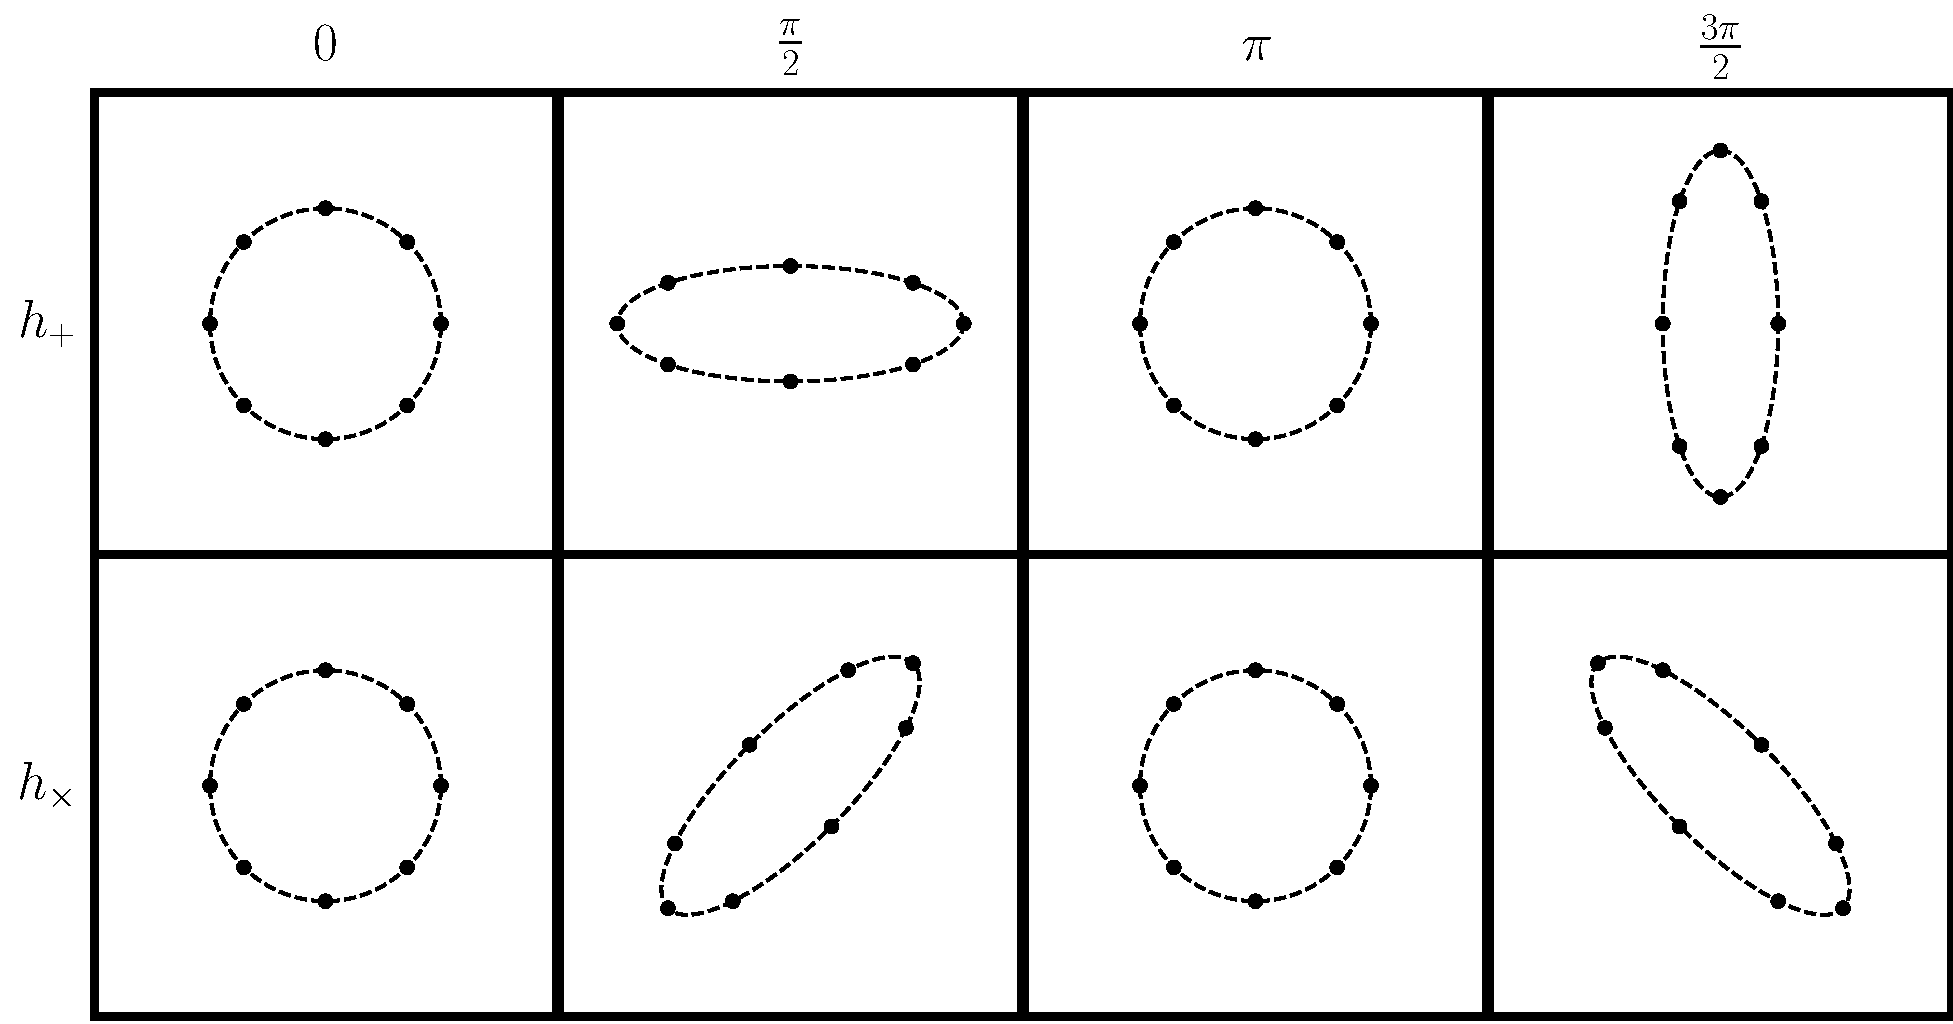
\includegraphics[width=\textwidth]{chapters/foundations/sections/gw/images/effect_gw.pdf}
	\caption[Effect of a gravitational wave on a ring of test-masses]{The effect of a \acrshort{gw} on a ring of freely falling test masses in the plane perpendicular to the propagation direction of the \acrshort{gw}. The two rows show the effect of the ``plus'' and ``cross'' polarization, respectively. The columns show different phases of the wave. The labels give the value of $\omega\tau$.}\label{fig:effect_gw}
\end{figure}

While the observable effects of a \acrshort{gw} can be studied by assuming vacuum solutions, their production cannot. To do so, the general solution of equation \eqref{eq:wave_eq_hbar} has to be considered, which is given by
\begin{equation}\label{eq:wave_solution_general}
\bar{h}_\mn\lr{t,\vec{x}}=\frac{4G}{c^4}\int \Diff{3}x'\ \frac{T_\mn\lr{t-\left|\left|\vec{x}-\vec{x}'\right|\right| /c,\vec{x}'}}{\left|\left|\vec{x}-\vec{x}'\right|\right|}.
\end{equation}
As the approximations underlying linearized gravity are only valid when there are at most small deviations from flat spacetime, we consider \eqref{eq:wave_solution_general} only far from the source of radiation. At large distances to the source the scale within the source is negligible and as such $\norm{\vec{x}-\vec{x}'}\approx\norm{\vec{x}}\eqqcolon r$. Using this approximation \eqref{eq:wave_solution_general} simplifies to
\begin{equation}
\bar{h}_\mn\lr{t,\vec{x}}=\frac{4G}{c^4}\frac{1}{r}\int \Diff{3}x'\ T_\mn\lr{t-r/c, \vec{x}'}.
\end{equation}
Projecting the equation into the \acrshort{tt} gauge and using that the energy-momentum tensor is divergence free, one finds~\cite{Maggiore:2008aaa}%page 109
\begin{equation}\label{eq:quadrupole-formula}
h^{\text{\acrshort{tt}}}_{ij}\lr{t, \vec{x}} = \frac{2G}{c^4}\frac{1}{r}\ddot{I}^{\text{\acrshort{tt}}}_{ij}\lr{t-r/c},
\end{equation}
where $\ddot{I}^{\text{\acrshort{tt}}}_{ij}$ is the second time derivative of the projection into the \acrshort{tt} gauge of the second mass moment
\begin{equation}
\ddot{I}^{ij} = c^2 \partial^2_0\int\Diff{3}x'\ x'^ix'^j T^{00}.
\end{equation}
The projection of this quantity is given by~\cite{Maggiore:2008aaa}%page 110
\begin{equation}\label{eq:I-tt-projection}
\ddot{I}^{\text{\acrshort{tt}}}=
\begin{pmatrix}
\lr{\ddot{I}_{11}-\ddot{I}_{22}}/2 & \ddot{I}_{12} & 0\\
\ddot{I}_{21} & -\lr{\ddot{I}_{11}-\ddot{I}_{22}}/2 & 0\\
0 & 0 & 0
\end{pmatrix}.
\end{equation}

The above equations can be used to approximate the gravitational radiation emitted by any mass distribution. Because this work considers only \acrshort{cbc} sources, we are interested in the \acrshort{gw}s sent out by two point particles orbiting each other. Due to the initial assumptions of linearized gravity, we are restricted to a separation of the two objects where the curvature of the background spacetime caused by the other object is small. In turn, however, this means that the orbital dynamics are governed by Newtonian dynamics and the problem reduces to the Kepler problem~\cite{Maggiore:2008aaa}. %page 120, 158
One solution to this problem are circular orbits, which can be described using an effective one body formalism with the reduced mass $\mu=\frac{m_1 m_2}{m_1 + m_2}$. From this setup the second time derivative of the second mass moment is calculated to be
\begin{equation}\label{eq:I-binary-point-masses}
\ddot{I}^{ij}=2\mu R^2 {\omega_s}^2
\begin{pmatrix}
\cos\lr{2\omega_s t} & \sin\lr{2\omega_s t} & 0\\
\sin\lr{2\omega_s t} & -\cos\lr{2\omega_s t} & 0\\
0 & 0 & 0
\end{pmatrix},
\end{equation}
where $R$ is the orbital separation of the two bodies and $\omega_s$ is their orbital frequency. In combination with \eqref{eq:quadrupole-formula} and \eqref{eq:I-tt-projection} this can be used to find the expressions for the polarizations of the \acrshort{gw}s. Interestingly, the frequency of \acrshort{gw}s originating from a binary system in circular orbits is exactly twice the orbital frequency. For eccentric orbits this property is lost \cite{Maggiore:2008aaa}.%page 182

The expressions obtained from the system described by \eqref{eq:I-binary-point-masses} are given in the frame of reference used to solve the Kepler problem. This means that we obtained the waves emitted in the $x^3$ direction from the center of mass. However, we are interested in the radiation emitted in all directions, as we cannot a priori know the orientation of a source with respect to our detectors. To resolve this issue, one needs to do one final projection which yields the waveform functions~\cite{Maggiore:2008aaa}%page 111
\begin{align}\label{eq:circular_orbit_waveforms}
h_+ & = \frac{4}{r}\frac{G}{c^4}\mu R^2 {\omega_s}^2\lr{\frac{1+\cos^2\lr{\iota}}{2}}\cos\lr{2\omega_s t + 2 \Phi}\nonumber\\
h_\times & = \frac{4}{r}\frac{G}{c^4}\mu R^2 {\omega_s}^2\cos\lr{\iota}\sin\lr{2\omega_s t + 2 \Phi},
\end{align}
where $\iota$ is the inclination of the system with respect to the line of sight and $\Phi$ is the orbital phase of the two objects at $t=0$.

Equation \eqref{eq:geodesic_deviation_gw} showed that \acrshort{gw}s can change the distance between particles. Therefore, the particles obtain kinetic energy from a passing \acrshort{gw} and stress can be induced in rigid bodies~\cite{Maggiore:2008aaa}. %page 26
As a consequence, \acrshort{gw}s must carry energy in order to pass it on. However, according to \eqref{eq:einstein}, if \acrshort{gw}s carry energy, they must act as a source of curvature themselves and the assumption \eqref{eq:linear_metric} of \acrshort{gw}s being a small perturbation in a flat background is not sufficient anymore. Instead one needs to consider a more general metric $g_\mn=\hat{g}_\mn+h_\mn$.

To obtain the energy carried by a \acrshort{gw} the background $\hat{g}_\mn$ must be separated from the \acrshort{gw} $h_\mn$. To achieve this we impose the condition that the background curvature fluctuates at most slowly compared to the rapidly oscillating $h_\mn$. In a rather lengthy calculation one can expand the Ricci tensor in terms of $h_\mn$ to second order. Taking the time average over multiple cycles of the \acrshort{gw} will then filter out its contribution to the curvature and leaves the background curvature behind. However, since terms quadratic in $h_\mn$ may have low frequency components, when the wave-vectors $\vec{k}_1$ and $\vec{k}_2$ are of similar magnitude but opposite sign, one can find that the \acrshort{gw} does have an influence on the background curvature. Since the background changes very slowly compared to the \acrshort{gw}, we can again view it as locally flat. Under these assumptions one can then write down an expression for the effective energy-momentum tensor of a \acrshort{gw}
\begin{equation}
t_\mn=\frac{c^4}{32\pi G}\langle\partial_\mu \lr{h^{\text{\acrshort{tt}}}}^{\sigma\alpha}\partial_\nu h^{\text{\acrshort{tt}}}_{\sigma\alpha}\rangle .
\end{equation}
A more thorough discussion of this derivation can be found in 1.4.2 of \cite{Maggiore:2008aaa}, where most of the above was paraphrased from, and 35.13 and 35.15 of \cite{Misner:1973aaa}.

Due to conservation of energy, the energy carried by the \acrshort{gw} must be taken away from the source. The main form of energy stored in the binary system studied above is the orbital energy. In turn, this means that the assumption of a constant circular orbit that led to the equations \eqref{eq:circular_orbit_waveforms} cannot hold. Instead one needs to consider the energy lost by gravitational radiation to calculate the phase of the \acrshort{gw}. 

The total energy carried away from the system is known as the luminosity and can be obtained by integrating the outwards pointing energy flux over a sphere with infinite radius. If we consider a binary system with large separation, where the orbital dynamics are well approximated by Newtonian theory, one finds
\begin{equation}\label{eq:luminosity_linear}
L_{\text{\acrshort{gw}}}=\frac{32}{5}\frac{c^5}{G}\lr{\frac{G\omega_s M_c}{c^3}}^{10 / 3}
\end{equation}
for the luminosity $L_{\text{\acrshort{gw}}}$, where
\begin{equation}
M_c\coloneqq \frac{\lr{m_1 m_2}^{3/5}}{\lr{m_1 + m_2}^{1/5}}
\end{equation}
is the chirp mass.

By setting the change in orbital energy equal to the luminosity and using Kepler's third law one can obtain a differential equation of the orbital frequency. This can be solved to get~\cite{Maggiore:2008aaa}%page 170
\begin{equation}
f_{\text{\acrshort{gw}}}\lr{\tau}=\frac{1}{\pi}\lr{\frac{5}{256}\frac{1}{\tau}}^{3/8}\lr{\frac{G M_c}{c^3}}^{-5/8},
\end{equation}
where $\tau$ is the time until the system merges. Integration yields the orbital phase
\begin{equation}
\Phi\lr{\tau} = -2\lr{\frac{5 G M_c}{c^3}}^{-5/8}\tau^{5/8}+\Phi_0,
\end{equation}
with $\Phi_0$ the phase at coalescence. To obtain the waveform, this expression could be inserted into the second mass moment, replacing $\omega_s t$. However, in the approximations that were used to derive the waveforms \eqref{eq:circular_orbit_waveforms} we assumed an almost flat background. As a consequence, the dynamics cannot be highly relativistic and the frequency will change slowly. Therefore, derivatives of the separation $R$ and the frequency $\omega_s = \pi f_{\text{\acrshort{gw}}}$ can be ignored to first order and we can approximate the waveforms by using Kepler's third law to replace $R$ by $\sqrt[3]{\frac{G M}{{\omega_s}^2}}$, $\omega_s$ in the prefactor of \eqref{eq:circular_orbit_waveforms} by $\pi f_{\text{\acrshort{gw}}}\lr{\tau}$, and $2\omega_s t + 2 \Phi$ in the argument of the cosine by $\Phi\lr{\tau}$. This yields
\begin{align}\label{eq:linear_waveform}
h_+\lr{\tau} & = \frac{1}{r}\lr{\frac{G M_c}{c^2}}^{5/4}\lr{\frac{5}{c\tau}}^{1/4}\lr{\frac{1+\cos^2\lr{\iota}}{2}}\cos\lr{\Phi\lr{\tau}}\nonumber\\
h_\times\lr{\tau} & = \frac{1}{r}\lr{\frac{G M_c}{c^2}}^{5/4}\lr{\frac{5}{c\tau}}^{1/4}\cos\lr{\iota}\sin\lr{\Phi\lr{\tau}}.
\end{align}

In \autoref{fig:linear_waveform} the $h_+$ polarization from \eqref{eq:linear_waveform} is plotted for $m_1=$\SI{35}{M_\odot}, $m_2=$\SI{30}{M_\odot}, $r=$\SI{1000}{\mega\parsec}.

\begin{figure}
	\centering
	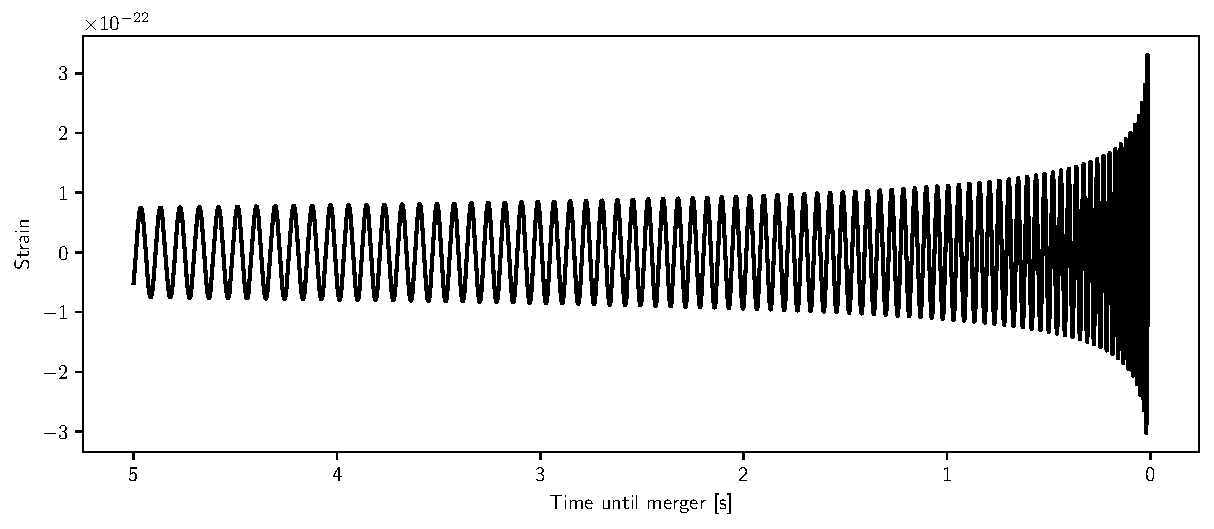
\includegraphics[width=\textwidth]{chapters/foundations/sections/gw/images/linear_waveform.pdf}
	\caption[Plus polarization waveform linearized gravity]{The strain of the plus polarization of a \acrshort{gw} as calculated by \eqref{eq:linear_waveform}. The parameters of the waveform are $m_1=$ \SI{35}{M_\odot}, $m_2=$ \SI{30}{M_\odot}, $r=$ \SI{1000}{\mega\parsec}, and $\iota, \Phi_0, \theta=0$.}\label{fig:linear_waveform}
\end{figure}


\subsection{Post-Newtonian Formalism}\label{sec:pn}
In the previous subsection the main approximation made to derive the gravitational radiation is the assumption of a flat background when describing the source dynamics. In other terms, we assumed that the orbital dynamics are governed by Newtonian dynamics and the background curvature is independent of the speed at which the bodies are orbiting. However, in a gravitationally bound system, the orbital velocity depends on the separation of the two bodies. More specifically, by the virial theorem one finds $\lr{v/c}^2\sim R_S/r$, where $R_S$ is the Schwarzschild radius and $r$ is the separation of the two objects~\cite{Maggiore:2008aaa}. %page 236
Therefore, the core assumption does not hold.

To treat gravitationally bound systems, one needs to consider a generic metric. However, solving the full Einstein equations is difficult and often impossible. One option to simplify problems are post-Newtonian (\acrshort{pn}) approximations~\cite{Misner:1973aaa}, %page 1069
where the full equations are expanded in a small parameter $\epsilon$. For binary systems, we use $\epsilon\sim\lr{v/c}$ and demand $\left|T^{ij}\right| / T^{00}=\mathcal{O}\lr{\epsilon^2}$, i.e. the source is at most weakly stressed~\cite{Maggiore:2008aaa}. %page 239
Requiring invariance of the equations under time-reversal the expansion works out to
\begin{align}
g_{00} & = -1 & & + g^{\lr{2}}_{00} & + g^\lr{4}_{00} & & + g^\lr{6}_{00} & & +\ \dots & \nonumber\\
g_{0j} & = & & & \phantom{+}g^\lr{3}_{0j}  & & + g^\lr{5}_{0j} & & +\ \dots & \\
g_{ij} & = & & \hspace{0.2cm}\phantom{+}\delta_{ij} & + g^\lr{2}_{ij} & & + g^\lr{4}_{ij} & & +\ \dots & ,\nonumber
\end{align}
where $g^\lr{n}$ denotes terms $\sim \epsilon^n$~\cite{Maggiore:2008aaa}. %page 239
To work consistently, when $g_{00}$ is expanded to order $n$, $g_{0i}$ must be expanded to order $n-1$ and $g_{ij}$ to order $n-2$~\cite{Maggiore:2008aaa}. %page 239
Similarly, the energy-momentum tensor also needs to be expanded
\begin{align}
T^{00} & = {T^\lr{0}}^{00} + {T^\lr{2}}^{00} + \dots\nonumber\\
T^{0j} & = {T^\lr{1}}^{0j} + {T^\lr{3}}^{0j} + \dots\\
T^{ij} & = {T^\lr{2}}^{ij} + {T^\lr{4}}^{ij} + \dots.\nonumber
\end{align}
To obtain approximations these expressions can be inserted into the Einstein equation \eqref{eq:einstein} and terms of the same order in $\epsilon$ can be equated. A solution is known to be of $n$-th \acrshort{pn}-order when terms up to order $\epsilon^{2n}$ are kept. Therefore, equations of $x.5$ \acrshort{pn}-order exist.

To 1 \acrshort{pn} order explicit solutions depending on the energy-momentum tensor are given in section 5.1.4 of \cite{Maggiore:2008aaa}, under the usage of the DeDonder gauge which in the full theory is given by
\begin{equation}
\partial_\mu\lr{\sqrt{-g}g^\mn}=0,
\end{equation}
where $g$ is the determinant of $g_\mn$. For the computation one also needs to consider that for $v/c\ll 1$ the time derivatives are smaller than the spatial derivatives by a factor $\mathcal{O}\lr{\epsilon}$ and hence the flat spacetime d'Alembert operator is given by
\begin{equation}\label{eq:pn_dalembert}
\Box = -\frac{1}{c^2}\frac{\partial^2}{\partial t^2}+\nabla^2 = \lr{1+\mathcal{O}\lr{\epsilon^2}}\nabla^2,
\end{equation}
where $\nabla^2=\delta^{ij}\partial_i\partial_j$. From this it is immediately clear that these solutions can only be valid close to the source, as they have to be instantaneous potentials~\cite{Maggiore:2008aaa}.%page 240

For further computations it is beneficial to cast the Einstein equations into their relaxed form
\begin{equation}\label{eq:relaxed_einstein}
\Box k^\mn = \frac{16 \pi G}{c^4}\tau^\mn,
\end{equation}
where $\Box$ is the flat spacetime d'Alembert operator,
\begin{equation}
k^\mn = \sqrt{-g}g^\mn-\eta^\mn,
\end{equation}
and
\begin{equation}
\tau^\mn=-gT^\mn + \frac{c^4}{16\pi G}\Lambda^\mn.
\end{equation}
The tensor $\Lambda^\mn$ captures the curvature contributions of the deviation from flat spacetime to the energy-momentum tensor~\cite{Blanchet:2006aaa} %page 16
and an explicit expression is given in (5.74) and (5.75) of \cite{Maggiore:2008aaa}. For \eqref{eq:relaxed_einstein} to be an exact equivalent to the Einstein equations \eqref{eq:einstein}, one also needs to enforce the DeDonder gauge which is given by $\partial_\nu k^\mn=0$ in this formulation.

To obtain a \acrshort{pn} expansion, we can then write the metric $k^\mn$ in a formal expansion of $v/c\approx 1/c$
\begin{equation}
k^\mn = \sum_{n=2}^\infty\frac{1}{c^n} k^\mn_n,
\end{equation}
where $v/c$ is the small parameter and only written for bookkeeping. As before, the right hand side of \eqref{eq:relaxed_einstein} must be expanded in the same manner~\cite{Maggiore:2008aaa}%page 261
\begin{equation}
\tau^\mn=\sum_{n=-2}^\infty\frac{1}{c^n}\tau^\mn_n.
\end{equation}
Inserting these expressions into the relaxed Einstein equation, using \eqref{eq:pn_dalembert}, and equating terms of the same order in $1/c$ we obtain the recursive equation
\begin{equation}
\nabla^2k^\mn_n = 16 \pi G \tau^\mn_{n-4} + \partial^2_t k^\mn_{n-2}.
\end{equation}
When solutions $k_0$ and $k_1$ are known, the right hand side of the above equation is fully determined and one needs to invert the Laplace operator $\nabla^2$ to obtain higher order \acrshort{pn} solutions.

This inversion, however, is not trivial, as the usual Poisson-integral diverges for high \acrshort{pn}-orders~\cite{Maggiore:2008aaa}. %page 261
Instead, one can find a particular solution for some finite \acrshort{pn}-order by multiplying the right hand side by $r^B$, for $B$ negative and large enough in magnitude. One can then consider the result in the complex plane and study the pole for $B\uparrow 0$, which is well defined and omits a solution. For the general solution the homogeneous solution has to be added. See 5.3.2 of \cite{Maggiore:2008aaa} and 5.2 of \cite{Blanchet:2006aaa} for more detail. Importantly, these solutions depend on the energy-momentum tensor of the source, but are only valid close to the source.

To get the radiation of the far field, we can consider the Post-Minkowskian (\acrshort{pm}) expansion. Since we are considering the region outside of the source, we are looking for vacuum solutions, i.e. $T^\mn=0$. In this case, the relaxed Einstein equation \eqref{eq:relaxed_einstein} simplifies to
\begin{equation}
\Box k^\mn = \Lambda^\mn.
\end{equation}
Outside the source the curvature will be small and we can expand in $R_s/r\sim G/r$. In a slight abuse of notation we write
\begin{gather}
k^\mn = \sum_{n=1}^\infty G^n k_n^\mn\\
\Lambda^\mn = N^\mn\left[k,k\right] + M^\mn\left[k,k,k\right]+\dotsc ,
\end{gather}
where $N^\mn$ and $M^\mn$ are tensors of quadratic and cubic order in $G$, respectively. Equating terms of the same order in $G$ leads to
\begin{equation}\label{eq:pm_wave_eq}
\Box k^\mn_n = \Lambda^\mn_n\left[k_1, \dotsc, k_{n-1}\right],
\end{equation}
where $\Lambda^\mn_n$ is the sum of all tensors $N^\mn,\ M^\mn,\ \dotsc$ of order $n$ in $G$.

In \eqref{eq:pm_wave_eq} we find another recursive relation, where higher order terms are determined from lower order ones. So once a solution $k^\mn_1$ is known, in principle all higher order solutions can be determined.

To find a solution to $k^\mn$ we observe that $\Lambda_1=0$ and write $k^\mn_1$ in a multipole expansion. Once the gauge condition is enforced, one can obtain solutions that depend on six families of multipole moments. See (5.95) to (5.101) in \cite{Maggiore:2008aaa} for explicit expressions. However, these multipole moments are still arbitrary functions, as they know nothing about the source of the radiation yet.

Iterating $k_1$ to find higher order solutions is again not trivial. In principle the right hand side of \eqref{eq:pm_wave_eq} is determined by all lower order solutions $k_1, \cdots, k_{n-1}$. So the task is in inverting the d'Alembert operator $\Box$. Notice that since the expansion is not in terms of $v/c$ anymore the d'Alembert operator must be inverted, rather than the Laplace operator. The solution to the problem is very similar to the solution used for the \acrshort{pn}-expansion. We find a particular solution by truncating the multipole expansion of $k^\mn_1$ at the desired order and multiply $\Lambda^\mn_n$ by $r^B$, with $B$ now positive and sufficiently large to cancel all factors $1/r$ in the multipole expansion. We then use the analytic continuation again and add the homogeneous solution to obtain the most general one. See 5.3.1 of \cite{Maggiore:2008aaa} or 4.1 of \cite{Blanchet:2006aaa} for more detail.

To determine the multipole moments of the \acrshort{pm} solutions, one observes that the \acrshort{pn} and \acrshort{pm} solutions have an overlapping region of validity~\cite{Blanchet:2006aaa}. Therefore, one uses the \acrshort{pn} solutions, which are determined by the energy-momentum tensor of the source, to fix the multipole moments of the \acrshort{pm} solutions. To do so, the \acrshort{pn} potentials are written as a multipole expansion and the \acrshort{pm} solitions are re-rexpanded in terms of powers of $1/c$. Finally, terms of the same order are equated. The explicit expressions are given in (85) - (90) of \cite{Blanchet:2006aaa}.

With this, the metric in the far region has in principle been determined. To find the actual waveform emitted by some physical system, one can follow a very similar approach to the one used in \autoref{sec:linear_gravity}. A binary system is well approximated by a sum of two delta functions\footnote{Using delta functions will actually lead to divergencies at high \acrshort{pn}-order. For this reason some regularization has to be applied. See section 8 of \cite{Blanchet:2006aaa} for details.} in the energy-momentum tensor. Using this energy-momentum tensor, one can find the metric in the near region of the source to determine the orbital energy $E$. On the other hand, it can be used to determine the metric in the far region, which can in turn be integrated to obtain the luminosity $L_{\text{\acrshort{gw}}}$ of the source. Under the assumption that the system loses energy only through gravitational radiation, we can use the equation
\begin{equation}
-\frac{\diff E}{\diff t} = L_{\text{\acrshort{gw}}}
\end{equation}
to obtain the orbital phase of the binary system.

For the case of linearized gravity discussed in \autoref{sec:linear_gravity} the orbital energy was known from Newtonian dynamics. In the \acrshort{pn} approximation it needs to be calculated. To do so, one inserts the \acrshort{pn} metric into the geodesic equation \eqref{eq:geodesic_equation} to obtain the equations of motion of the two orbiting bodies. From this one can find the orbital energy. Explicit expressions can be found in \cite{Blanchet:2006aaa}, equation (115) gives the generic metric to $3$ \acrshort{pn}-order, (168) gives the equation of motion of a binary system to $3.5$ \acrshort{pn}-order, (170) gives the orbital energy to $3$ \acrshort{pn}-order, and (194) gives the energy to $3$ \acrshort{pn}-order assuming circular orbits.

The luminosity can be directly computed from the metric by integration. See section 3.5 of \cite{Maggiore:2008aaa} or section 6 and section 10.2 of \cite{Blanchet:2006aaa} for details. Explicit expressions at $3.5$ \acrshort{pn}-order are given in (5.257) of \cite{Maggiore:2008aaa} and (231) of \cite{Blanchet:2006aaa}. The resulting phase to $3.5$ \acrshort{pn}-order is given in (235) of \cite{Blanchet:2006aaa}.

To obtain the waveform, one can project the metric $g_{ij} - \delta_{ij}$ into the \acrshort{tt}-frame. The metric $g_{ij}$ is the desired \acrshort{pn}-approximation, the derivation of which was discussed above. The polarizations can be read of. Explicit expressions were derived in \cite{Blanchet:1996pi, Arun:2004ff} and can be found in (237) - (241) of \cite{Blanchet:2006aaa}. To get the actual waveform, the time dependent phase to highest known \acrshort{pn}-order should be inserted.

The discussion above is meant as a high-level overview of how \acrshort{pn}-waveforms can be obtained. A more detailed overview, including mathematical details, is given in \cite{Blanchet:2006aaa}. Notably, this discussion excluded spin effects of the binary system and its constituents. Discussions including spin can be found for instance in \cite{Damour:2001tu, Blanchet:2004ek, Faye:2006gx, Blanchet:2006gy, Damour:2007nc}.


\subsection{Waveform Models}
The waveforms discussed in subsections \ref{sec:linear_gravity} and \ref{sec:pn} are, by construction, only valid during the inspiral, even though high order \acrshort{pn} waveforms remain accurate until a few cycles before the merger of the two objects~\cite{Blanchet:2006aaa, Santamaria:2010yb}. %page 85, last paragraph
However, the emitted energy scales to high power with the orbital frequency of the two merging objects, as can be seen from \eqref{eq:luminosity_linear} to linear order and from (231) of \cite{Blanchet:2006aaa} to $3.5$ \acrshort{pn}-order. Therefore, the evolution of the waveform close to merger can be of high importance for detection.

This subsection gives an overview of the three most prominently used waveform-model families and their variants. All of them model the entire orbital evolution from inspiral, over merger, to ringdown (\acrshort{imr}), in the parameter regions where they are valid. To be able to represent the merger phase, all of them rely on numerical relativity (\acrshort{nr}) simulations, which solve the Einstein equations numerically. These simulations are the most accurate tools available to solve the highly non-linear interactions but running them requires enormous amounts of computational power. Generating a waveform encompassing the final few orbits and the merger for a single binary system using \acrshort{nr} can take days or even weeks, depending on the initial conditions and type of binary system~\cite{Hannam:2009rd}. Therefore, it is often not viable to use the resulting waveforms in data analysis methods discussed in section \ref{sec:cbc_searches} directly. The waveform models below are constructed to overcome this issue by combining the accurate \acrshort{nr} waveforms with analytical approximations.

Instead of writing the \acrshort{gw} polarizations as individual functions, one can also define a single complex strain
\begin{equation}
H\coloneqq h_+ + i h_\times,
\end{equation}
which can be decomposed using spherical harmonics~\cite{Thorne:1980ru, Dhurkunde:2022aek}
\begin{equation}\label{eq:complex_waveform}
H=\sum_{l\geq 2}\sum_{m=-l}^l Y^{-2}_{lm}\lr{\iota, \Phi_0}h_{lm}\lr{\tau, r, \kappa},
\end{equation}
where
\begin{equation}
h_{lm}\lr{\tau, r, \kappa} = A_{lm}\lr{\tau, r, \kappa} e^{-i\Phi_{lm}\lr{\tau, \kappa}}.
\end{equation}
$\kappa$ represent all parameters that describe the source itself and which do not depend on the location at which one observes the radiation. Waveform models usually describe the amplitude evolution $A_{lm}$ and the phase evolution $\Phi_{lm}$. If a waveform model is capable of modeling these quantities for $(l, m) \neq (2, \pm 2)$, one speaks of a model that is capable of simulating higher order modes (\acrshort{hm}).


\subsubsection{Effective One-Body Waveform-Family}
Effective one body (\acrshort{eob}) waveforms were one of the first \acrshort{gw} approximants that could model not only the inspiral but also the merger and ringdown. The formalism was introduced in \cite{Buonanno:1998gg} and maps the two body problem of a \acrshort{bbh} system onto that of a test particle moving in an effective external metric. To that end, a Hamiltonian is constructed which is supplemented with a radiation-reaction force. It takes the \acrshort{pn} approximation as a starting-point to express the Hamiltonian and then expresses it as well as the radiation-reaction force in a resummed form, where the functions are non-polynomial~\cite{Damour:2008te}. An introduction to the resummation is given in 14.1 of \cite{Maggiore:2018aaa}. This resummation can then be extended by adding free parameters that model non-perturbative effects~\cite{Damour:2001tu, Damour:2002vi, Damour:2007xr}. The \acrshort{eob} formalism models the inspiral and merger by fitting the free parameters to \acrshort{nr} and then attaches an analytical model for the ringdown.

The first full \acrshort{imr} waveform from the \acrshort{eob} family was derived in \cite{Buonanno:2000ef}. Initially it modeled only non-spinning \acrshort{bbh}s but was later extended to the spinning case in \cite{Buonanno:2005xu, Barausse:2009aa}. The early models were solely based on analytic calculations. However, with the breakthrough in \acrshort{nr} in 2005~\cite{Maggiore:2018aaa, Pretorius:2005gq, Campanelli:2005dd, Baker:2005vv} accurate ground-truths became available, which could be used to constrain the free parameters that extend the \acrshort{eob} models~\cite{Buonanno:2007pf, Damour:2008te}. These models were incrementally improved~\cite{Damour:2009kr, Buonanno:2009qa} and extended to include higher order modes, aligned spins, and precession~\cite{Barausse:2009xi, Pan:2009wj, Pan:2011gk, Pan:2013rra}. To keep track of the capability of these models, a naming scheme was introduced. Waveforms of this family carry an ``\acrshort{eob}'' in their name, which is usually followed by ``\acrshort{nr}'' to signify that the model coefficients were tuned to \acrshort{nr} simulations. A leading ``S'' informs the user about the capability of the model to represent (anti-)aligned spins. Afterwards a version number is tagged onto the string. The first model named this way is known as ``SEOBNRv1'' and was introduced in \cite{Taracchini:2012ig}, ``SEOBNRv2'' is the model described in \cite{Taracchini:2013rva, LIGOScientific:2016vlm}, ``SEOBNRv3'' the one described in \cite{Pan:2013rra, LIGOScientific:2016vlm}, and ``SEOBNRv4'' in \cite{Bohe:2016gbl}. At the time of writing, the \acrshort{eob} model that encompasses the most orbital dynamics is ``SEOBNRv4PHM'', which can account for higher order modes and precession at the same time~\cite{Ossokine:2020kjp}. The \acrshort{eob} models are formulated as a set of differential equations, that need to be solved for given parameters, which can be prohibitively slow depending on the application~\cite{LIGOScientific:2016vlm}. They are also formulated in the time domain, wheras data analysis usually requires the waveform in the frequency domain. For these reasons, \acrshort{eob} models are often sped up by building reduced order models in the frequency domain~\cite{Purrer:2014fza, Purrer:2015tud}.


\subsubsection{Phenom Waveform-Family}
The phenomelogical -- short Phenom -- waveform-family was introduced in \cite{Ajith:2007qp}. At the core, their method matches the analytic \acrshort{pn}-waveform that describes the inspiral with the more accurate \acrshort{nr}-waveform during merger to produce a finite amount of hybrid waveforms. Afterward, the hybrid waveforms are fit to a phenomenological parametrized model which can in turn be mapped to the physical parameters of the binary system~\cite{Santamaria:2010yb}. The resulting model is fast to evaluate, highly accurate, and usually native to the frequency domain.

Since the initial paper, which focused on non-spinning \acrshort{bbh}s in a mass range of \SI{30}{M_\odot} to \SI{130}{M_\odot}, many different versions of the waveform model have been released. The work of \cite{Ajith:2009bn} introduced a Phenom-waveform model that is capable of modeling \acrshort{bbh}s, the spins of which are (anti-)aligned with the orbital angular momentum. Through \cite{Schmidt:2012rh, Hannam:2013oca} waveform models that can take precession effects of the emitting binary into account were introduced and dubbed PhenomP, where the ``P'' signifies the ability to represent precessing systems. The PhenomP model was used during data analysis of the first detected \acrshort{gw}~\cite{LIGOScientific:2016aoc, LIGOScientific:2016vlm, LIGOScientific:2019hgc}. The authors of \cite{London:2017bcn} introduced a model that can account for higher multipoles (``PhenomHM''), which was combined with an updated version of the precessing waveform model~\cite{Khan:2018fmp} to obtain a waveform model that can represent both effects~\cite{Khan:2019kot} (``PhenomPv3HM''). The underlying model was also revised multiple times over the years. The evolving non-precessing approximants were called ``PhenomB''~\cite{Ajith:2009bn}, ``PhenomC''~\cite{Santamaria:2010yb}, and ``PhenomD''~\cite{Husa:2015iqa, Khan:2015jqa}. The most recent version, skipping many letters in between, is the ``PhenomX'' waveform model~\cite{Pratten:2020fqn}, which has a version that allows for the computation of higher order multipoles called ``IMRPhenomXHM''~\cite{Garcia-Quiros:2020qpx}, and a version that includes both higher order multipoles and precession effects, known as ``IMRPhenomXPHM''~\cite{Pratten:2020ceb}. The prefix ``IMR'' signifies that the waveform models the full inspiral-merger-ringdown. The postfix ``HM'' signifies that higher order multipoles can be computed.


\subsubsection{Numerical Relativity Surrogate Waveform-Family}
By now hundreds of \acrshort{nr} simulations are available that span large parts of the expected parameter space for \acrshort{bbh} mergers~\cite{Boyle:2019kee, Healy:2022wdn}. The resulting waveforms are the most accurate predictions of the emitted radiation of a merging binary system that are available to us. \acrshort{nr} surrogate models leverage the existing catalogs of \acrshort{nr} simulations to interpolate between them. They are typically more accurate than the approximate methods described above but are only valid in the limited parameter regions that are covered by the underlying simulations~\cite{Setyawati:2019xzw}.

The first surrogate model was introduced in \cite{Blackman:2015pia} and used non-spinning waveforms produced by the Spectral Einstein Code~\cite{Scheel:2014ina, Szilagyi:2014fna}. The model was later extended to include precession~\cite{Blackman:2017dfb} and more parameters~\cite{Blackman:2017pcm, Varma:2018aht}. Currently the model named ``NRSur7dq4''~\cite{Varma:2019csw} is used in state-of-the-art analyses~\cite{LIGOScientific:2021djp}, where ``7dq4'' signifies that the model is valid for a $7$ dimensional parameter space (6 spins + mass ratio) up to a mass ratio $q$ of $4$.

\section{Data Analysis for Compact Binary Coalescence Signals}\label{sec:cbc_searches}
The observable changes that \acrshort{gw}s induce in detectors are very small, as we will see in section \ref{sec:detectors}. Consequently, detecting them directly is a difficult problem that stood unsolved for nearly a century.

The first indirect detection of \acrshort{gw}s was made in 1982 when Joseph H. Taylor and Joel M. Weisberg closely studied the pulsar PSR 1913+16~\cite{Taylor:1982zz}. Said pulsar was discovered in 1974 and was the first one that was part of a binary system~\cite{Hulse:1974eb}. It became known as the Hulse-Taylor pulsar, named after the researchers who discovered it. A pulsar is a rotating \acrshort{ns} that emits a beam of radiation. If the beam continuously sweeps across a detector, it appears as a periodic signal. The frequency of these pulses is known to be extremely stable~\cite{Matsakis:1997aaa, Verbiest:2009aaa} and, consequently, allows to trace the orbit of pulsars in binaries very accurately. As was discussed in section \ref{sec:gw_main}, a binary of compact objects emits considerable amounts of energy as gravitational radiation and subsequently slowly spirals together. The change in orbit for the Hulse-Taylor pulsar due to energy lost in \acrshort{gw}s was calculated and then checked against measurements~\cite{Taylor:1982zz, Weisberg:2004hi}. The observed change in the orbital period matches the theoretical predictions from \acrshort{gr} to an astonishing accuracy.

Although this indirect detection was strong evidence for the existence of \acrshort{gw}s, it was no direct detection. It could not be ruled out that some other unaccounted-for effect caused the change in the orbital period. To confirm the observation, a direct detection of the physical effects of \acrshort{gw}s was sought.

Initial efforts toward a direct detection were made by Joseph Weber in the 1960s~\cite{Maggiore:2008aaa, Weber:1960zz}. %page 415
He tried to measure resonances in an aluminum bar induced by the gravitational radiation. In 1969 he claimed to have detected a \acrshort{gw}~\cite{Weber:1968llz, Weber:1969bz} but his findings were not reproducible and subsequently dismissed~\cite{Pitkin:2011yk}. %Section 3.1
For details on resonant bar detectors and their response to \acrshort{gw}s see chapter 8 of \cite{Maggiore:2008aaa}.

The first confident detection of a \acrshort{gw} was made by the LIGO-Virgo collaboration (\acrshort{lvc}) on September 14, 2015~\cite{LIGOScientific:2016aoc}. Since then, $\mathcal{O}(100)$ observations were reported by several groups analyzing the public data~\cite{LIGOScientific:2019lzm} that has been recorded in three observation periods~\cite{LIGOScientific:2021djp, Nitz:2021zwj, Venumadhav:2019tad, Venumadhav:2019lyq, Olsen:2022pin}. The data was recorded by three earth bound detectors \acrshort{ligo} Livingston, \acrshort{ligo} Hanford~\cite{LIGOScientific:2014pky}, and Virgo~\cite{VIRGO:2014yos}. Toward the end of the last observing period, a fourth detector -- KAGRA~\cite{KAGRA:2018plz} -- joined the network. All of them are kilometer scale laser interferometers, of which a brief introduction will be given in subsection \ref{sec:detectors}.

A lot of new insights into the Universe can be drawn from these observations. One of the most prominent studies are tests of \acrshort{gr}~\cite{LIGOScientific:2016lio, LIGOScientific:2021sio, Shoom:2021mdj, Krishnendu:2021fga}. So far, no evidence for a deviation from \acrshort{gr} has been found. Other insights that can be obtained from \acrshort{gw} observations include constraints on the equation of state of \acrshort{ns}~\cite{LIGOScientific:2018cki, Capano:2019eae}, the Hubble-constant~\cite{LIGOScientific:2018gmd, DES:2019ccw}, the population of \acrshort{bh}s~\cite{LIGOScientific:2021psn}, and the fraction of dark matter explainable by \acrshort{bh}s~\cite{Sasaki:2018dmp, LIGOScientific:2021job, Basak:2021ten}. They can also help explain how \acrshort{bh}s and other systems form \cite{Broekgaarden:2021hlu}. The list of possible applications goes on and keeps growing as our understanding of the Universe improves.

Nonetheless, to make any of these claims, \acrshort{gw}s must first be identified and characterized in the detector data. In subsection \ref{sec:detectors}, we will see that noise dominates the raw output data of the detectors. Sophisticated data analysis methods were developed to extract the weak signals from the raw data. The \acrshort{ligo}-Virgo-KAGRA collaboration (\acrshort{lvk}) deploys a suite of different algorithms to detect potential signals in the data~\cite{LIGOScientific:2021djp}, which can be classified into two categories based on their underlying search strategy. GstLAL~\cite{Messick:2016aqy, Sachdev:2019vvd, Hanna:2019ezx, Cannon:2020qnf}, MBTA~\cite{Adams:2015ulm, Aubin:2020goo}, and PyCBC~\cite{Allen:2005fk, Usman:2015kfa, Nitz:2017svb, Nitz:2018rgo, Davies:2020tsx} are search pipelines that filter the data against a set of pre-computed waveforms. They are often called modeled searches and I will describe their core concept ``matched filtering'' in subsection \ref{sec:matched_filtering}. Coherent wave burst (cWB)~\cite{Klimenko:2004qh, Klimenko:2011hz, Klimenko:2015ypf, Mishra:2022ott} is a loosely modeled search pipeline that makes minimal assumptions about the source and looks for coherent excess power in multiple detectors to detect transient events.

When accurate models of the signal exist, modeled searches are more sensitive than loosely modeled searches. However, modeled searches can only target a fixed range of parameters of binary systems, which has to be chosen before the data is searched. Since the computational cost of these searches scales with the searched parameter space, one has to make compromises between search space and runtime. As a consequence, signals from sources with unexpected or unlikely parameters may be missed. The modeled searches that are used in the studies that have identified all known signals to date~\cite{LIGOScientific:2021djp, Nitz:2021zwj, Venumadhav:2019lyq, Olsen:2022pin} assume circular orbits, aligned spins, and only search the mass range from \SI{1}{M_\odot} to \SI{758}{M_\odot}. They also put constraints on the mass ratio and assume that higher order modes have a negligible effect on the observed waveform. Several specialized searches targeting eccentric systems~\cite{Lenon:2021zac}, large higher order mode contributions~\cite{Chandra:2022ixv}, or sub-solar mass systems~\cite{LIGOScientific:2019kan, Nitz:2020bdb, Nitz:2021mzz, Nitz:2021vqh, Nitz:2022ltl} have been carried out, none of which have found any new signals. Most importantly to this thesis, machine learning search algorithms are starting to be explored to reduce computational costs and widen the parameter space that can be searched~\cite{George:2016hay, Schafer:2020kor, Cuoco:2020ogp, Wei:2020ztw, Schafer:2022dxv}. A more detailed discussion of these approaches is given in section \ref{sec:ml-gw-hist} and chapters \ref{ch:bns}, \ref{ch:training_strats}, \ref{ch:cnn_coinc}, and \ref{ch:mlgwsc1}.

\subsection{Noisy Detector Data}\label{sec:detectors}
At the time of writing, five laser interferometer \acrshort{gw} detectors are operational. These include the \acrshort{ligo} detectors~\cite{LIGOScientific:2014pky} in Livingston (Louisiana, USA) and Hanford (Washington, USA), the Virgo detector~\cite{VIRGO:2014yos} in Cascina (Italy), the KAGRA detector~\cite{KAGRA:2018plz} in Kamioka (Gifu, Japan), and the GEO 600 detector~\cite{Luck:2010rt, Affeldt:2014rza, Dooley:2015fpa} in Sarstedt (Germany).

The \acrshort{ligo} and Virgo detectors are already sensitive enough to regularly detect \acrshort{gw}s during operation~\cite{LIGOScientific:2021djp}. KAGRA was only taken into service recently and has not yet reached a level of sensitivity where detections are likely~\cite{KAGRA:2022twx}. It is expected to reach its sensitivity targets during the fourth observing run (\acrshort{o4})~\cite{KAGRA:2018plz}. GEO 600 is unlikely to ever reach a sensitivity where it can regularly detect \acrshort{gw}s, due to the size of the detector. It is, therefore, used as a testbed for new technologies that transition to the other detectors once they have proven to yield improvements~\cite{GEO:2022aaa}.

At their core all of these instruments are highly advanced Michelson interferometers, which split a laser beam into two orthogonal beams. Each beam travels along the arm of the interferometer until it is reflected back by a mirror at the end of the arm. When the beams recombine at the beamsplitter, they interfere and the output power depends on the difference of the distance the light has traveled in both arms. Due to the short wavelengths of light, this allows to measure very small changes in the differential arm lengths~\cite{Demtroder:1995aaa}. %page 306

As discussed in section \ref{sec:gw_main}, \acrshort{gw}s cause a physical displacement of test masses with respect to some reference point. In the \acrshort{gw} detectors, the mirrors at the end of the arms act as test masses and the beamsplitter as the point of reference. Therefore, the Michelson interferometer is sensitive to \acrshort{gw}s. Under the assumption that the arm length $L$ of the interferometer is small compared to the wavelength of the \acrshort{gw}, from equation \eqref{eq:geodesic_deviation_gw} one finds to first order that the change in arm length $\Delta L$ is given by
\begin{equation}
L + \Delta L = L \lr{1 + \frac{h_+}{2}},
\end{equation}
when only the $+$ polarization is considered and the source is optimally located. Therefore, in order to amplify the effect of a \acrshort{gw} on the detector, one can increase the arm length $L$. Another option to increase the measured signal is to increase the power that circulates in the arms or install a Fabry-Perot cavity \cite{Maggiore:2008aaa}. For these reasons, the \acrshort{ligo} and Virgo detectors have arm lengths of \SI{4}{\kilo\metre} and \SI{3}{\kilo\metre}, respectively, and circulate several hundred \SI{}{\kilo\watt} of laser power in the Fabry-Perot cavities of their arms. KAGRA also has an arm length of \SI{3}{\kilo\metre} but is built underground and cryogenically cools its mirrors. GEO 600 has an arm length of \SI{600}{\metre}. \autoref{fig:detector_diagram} shows a high level overview of current detectors.

\begin{figure}
	\centering
	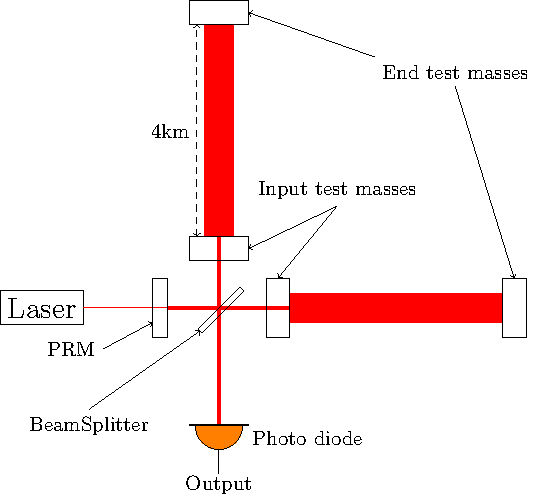
\includegraphics[width=0.5\textwidth]{chapters/foundations/sections/cbc_searches/images/michelson_interferometer.pdf}
	\caption[Diagram of a laser interferometer gravitational-wave detector]{The figure shows a simplified diagram of the interferometric \acrshort{gw} detectors. The diagram is not to scale and only highlights the beam path. Any operations for stabilization, mode cleaning, and so on are not shown. The laser beam travels from the laser through the power recycling mirror (PRM) to the beam splitter, where it is split into equal parts to the two arms. In each arm, the beam passes an input test mass, which is a mirror, travels \SI{4}{\kilo\metre}, and is reflected at the end test mass. On its way back, a large portion of the light is again reflected by the input test mass to increase the light travel time in the arms. Together the two test masses essentially create a large Fabry-Perot cavity. Once the light passes the input test mass, it recombines and interferes with the light from the other arm. A photodiode captures the beam at the output port (south) to produce the readout. The part going back to the laser is reflected at the power recycling mirror to increase the laser power in the interferometer. This figure was adapted from Figure 1 in \cite{LIGOScientific:2014pky}.}\label{fig:detector_diagram}
\end{figure}

To obtain the length deviation, one can in principle use equation \eqref{eq:geodesic_deviation_gw} as discussed above. However, that equation is in a frame of reference in which the effect of \acrshort{gw}s on test masses can be easily described and where the $x^3$ direction points from the source to the detector. The frame of reference of the detector, on the other hand, defines the $x$- and $y$-axis as the arms of the detector and the $z$-axis such that it is orthogonal to the $x$-$y$-plane pointing away from the center of the earth. To translate the motion in one frame to the motion in the other frame, one can use a transformation based on Euler-rotations. Carrying out these calculations leads to~\cite{Schutz:2011tw}
\begin{align}\label{eq:delta_l}
h = & \phantom{+}F_+\lr{\theta, \varphi}\lr{\cos\lr{2\psi}h_+ - \sin\lr{2\psi} h_\times}\nonumber\\
& + F_\times\lr{\theta, \varphi}\lr{\sin\lr{2\psi}h_+ + \cos\lr{2\psi} h_\times},
\end{align}
where $\theta$, $\varphi$, and $\psi$ are the Euler-angles known as declination, right ascension, and polarization angle, respectively, and
\begin{align}\label{eq:antenna_patterns}
F_+\lr{\theta, \varphi} & = \frac{1}{4}\lr{3+\cos\lr{2\theta}}\sin\lr{2\varphi}\nonumber\\
& = \frac{1}{2}\lr{1 + \cos^2\lr{\theta}}\sin\lr{2\varphi},\nonumber\\
F_\times\lr{\theta, \varphi} & = \cos\lr{\theta}\cos\lr{2\varphi}.
\end{align}

In total, the \acrshort{gw}s the detectors measure depend on $15$ parameters for \acrshort{bbh} signals and $17$ for \acrshort{bns} systems. An overview of these parameters is given in \autoref{fig:gw_params}. They affect the measured signal in different ways:
\begin{description}
	\item[$\bm{m_1, m_2}$] The component masses of the two objects. Usually it is defined that $m_1\geq m_2$. To leading order they are the only parameters that influence the frequency evolution of the signal and they act mainly through the mass combination known as the chirp mass. The larger the total mass of the system, the lower the frequency at which the two objects merge.
	\item[$\bm{\vec{\chi}_1, \vec{\chi}_2}$] The three-dimensional spin vectors of the individual objects. They often are only measured in a mass-weighted form known as the effective spin $\chi_e$~\cite{Schmidt:2012rh} and the effective precession spin $\chi_p$~\cite{Schmidt:2014iyl}. As long as the spins are (anti-)aligned with the orbital angular momentum, they affect the time scale at which the objects merge. The more aligned the spin, the longer the time scale. If they are not aligned with the orbital angular momentum they cause precession effects, that become visible as a beating in the signal.
	\item[$\bm{\Lambda_1, \Lambda_2}$] Tidal deformabilities of the two objects. They quantify the amount of matter distortion due to the gravitational gradient in the close proximity to a highly compact object. Subsequently they are $0$ for \acrshort{bh}s and are only considered for \acrshort{bns} and \acrshort{nsbh} mergers. The larger the tidal deformability, the stiffer the \acrshort{ns}, and the longer the duration of the inspiral. However, the influence of matter effects are expected to be very small and they have not been measured yet~\cite{LIGOScientific:2021djp}.
	\item[$\bm{r}$] The distance from the source to the detector. It is inversely proportional to the amplitude of the waveform measured in the detector.
	\item[$\bm{\theta, \varphi}$] The declination $\theta$ and the right ascension $\varphi$ in the reference frame of the detector. They affect the amplitude of the measured signal through \eqref{eq:delta_l} to the point where the detectors can be blind to specific polarizations from given locations in the sky. \autoref{fig:sky_location_influence} shows the average influence of the sky position on the strength of the detected signal.
	\item[$\bm{\Psi}$] The polarization angle. It is the angle by which the frame of the \acrshort{gw} has to be rotated around the propagation axis to line up with the frame of the detector. For a single detector it can be absorbed into a redefinition of the two polarizations of the wave and cannot be resolved. See \autoref{fig:gw_params} for a visualization of this angle.
	\item[$\bm{\iota}$] The inclination of the orbital plane of the source with respect to the line of sight of the detector. It influences the radiated power and, therefore, the amplitude of the signal. A plot of the power distribution is shown in \autoref{fig:angle_power}.
	\item[$\bm{\Phi_0}$] The coalescence phase, i.e. the orbital position of the two objects at merger. It introduces an overall phase-shift in the measured signal.
	\item[$\bm{t_0}$] The time of coalescence, which is often defined as the time at which the merger signal arrives at the center of the earth. Controls the time at which the system merges and time shifts the waveform in the detector data.
\end{description}

\begin{figure}
	\centering
	\begin{subfigure}[b]{.72\linewidth}
		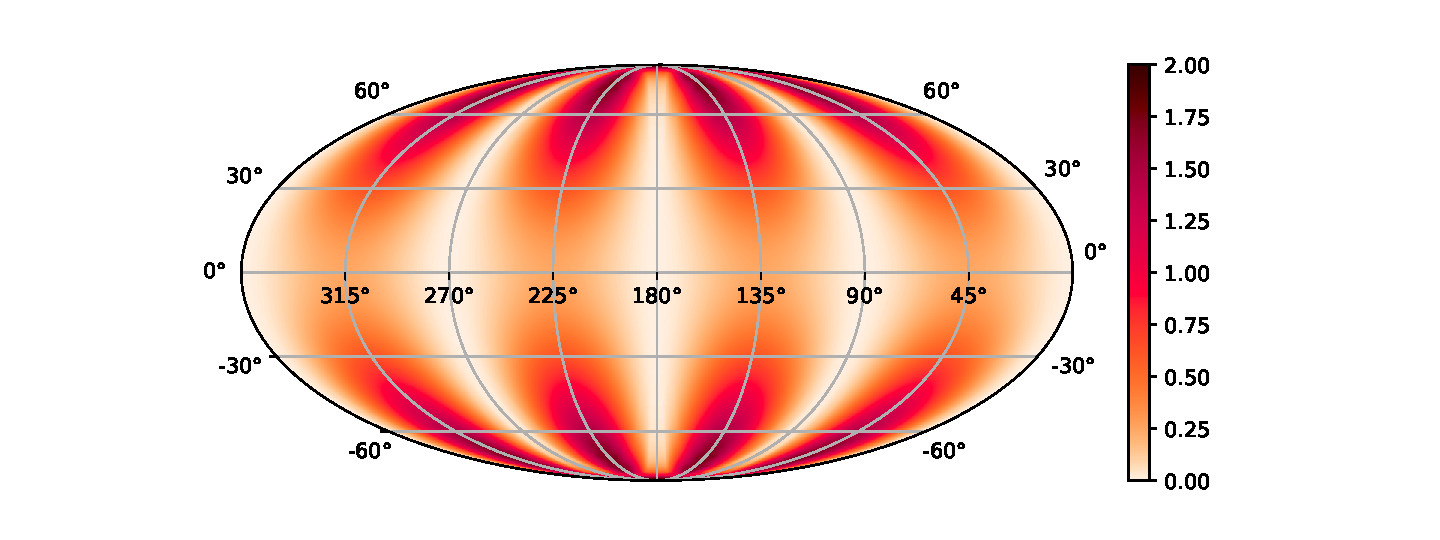
\includegraphics[width=\linewidth]{chapters/foundations/sections/cbc_searches/images/sky_location_power.pdf}
		\caption{Sky location}\label{fig:sky_location_influence}
	\end{subfigure}
	\begin{subfigure}[b]{.27\linewidth}
	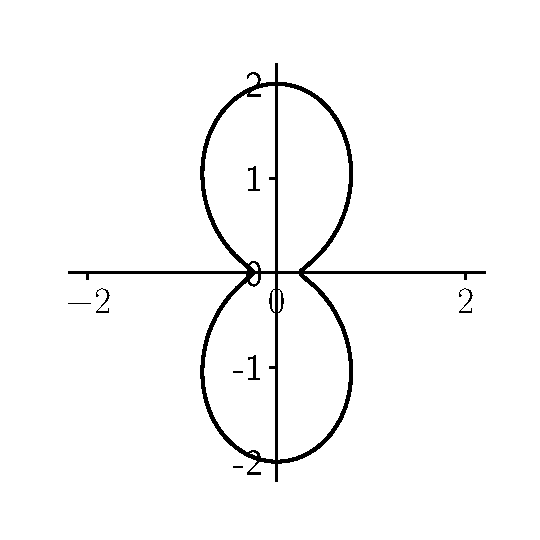
\includegraphics[width=\linewidth]{chapters/foundations/sections/cbc_searches/images/angular_power_distribution.pdf}
	\caption{Inclination}\label{fig:angle_power}
	\end{subfigure}
	\caption[Gravitational wave angular power distributions]{\textbf{(a) Sky location:} The influence of the sky-position on the \acrshort{gw} intensity observed by the detector averaged over all source orientations. It is known as the antenna power function and we observe that there are favorable and unfavorable sky-locations for the detectors. This figure was inspired by Figure 2 of \cite{Schutz:2011tw}. \textbf{(b) Inclination:} The multiplicative factor of the radiated power of a \acrshort{gw}. The angle to the x-axis is the inclination of the system, the distance to the origin gives the factor by which the radiated power from the source intrinsic parameters has to be multiplied. This shows that face-on systems ($\iota=\pi/2$ or $\iota=3\pi/2$) are seen with the highest intensity, while edge-on systems ($\iota=0$ or $\iota=\pi$) are observed with the lowest intensity. However, it also shows that there is no dead-spot and some power is radiated in all directions. This figure was adapted from Figure 3.7 of \cite{Maggiore:2008aaa}}
\end{figure}
\begin{figure}
	\centering
	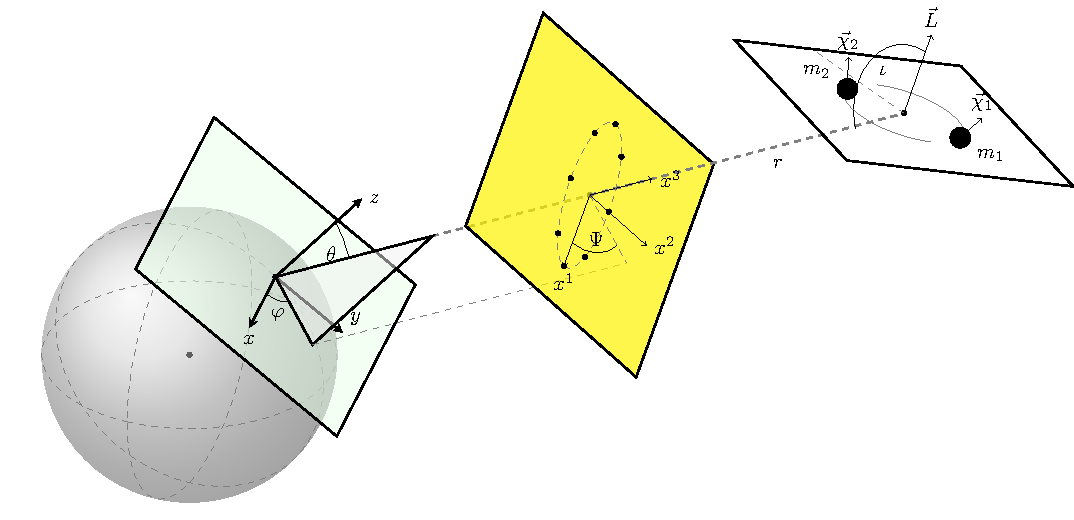
\includegraphics[width=\textwidth]{chapters/foundations/sections/cbc_searches/images/gw_params.pdf}
	\caption[Gravitational wave signal parameters]{A diagram showing the parameters the measured signal of a \acrshort{bbh} merger depends on. The three differently colored planes indicate the three different coordinate systems used in the calculation of the \acrshort{gw} effect. The white plane belongs to the source. It is aligned with the orbital plane. The yellow frame shows the preferred frame of reference for a \acrshort{gw}, where its propagation direction is aligned with the $x^3$-axis. The deformed ellipsoid on the plane indicates the movement of a ring of test masses in this frame (compare \autoref{fig:effect_gw}). The green plane shows the frame of the detector, where the $x$- and $y$-axes are aligned with the detector arms and $z$ points away from the center of the earth, which is depicted as the gray sphere. The angles show the transformations that are associated with them. The distance $r$ is highlighted by the dashed gray line connecting the detector and the source. Not shown are the time of coalescence $t_0$ and the coalescence phase $\Phi_0$. $\vec{L}$ shows the orbital angular momentum. The figure is not to scale and only meant to show the meaning of the different parameters. It was inspired by Figure 9.2 of \cite{Hawking:1989aaa}.}\label{fig:gw_params}
\end{figure}

Equation \eqref{eq:delta_l} describes the signal the detector would pick up in an ideal environment. However, as we all know the world around us is not an ideal environment, as it is noisy. To get a sense of scale at which noise sources have to be considered, one can estimate the length change induced by a \acrshort{gw} on an interferometric detector with arms at a right angle and \SI{4}{\kilo\metre} length. Using \eqref{eq:linear_waveform} for a non-spinning, face-on system ($\iota=0$) at a distance $r$ of \SI{1}{\giga\parsec} with masses similar to those of the first observed \acrshort{gw} directly overhead the detector yields a length deviation of $\approx$ \SI[parse-numbers=false]{10^{-18}}{\metre}. At these length scales almost any noise source is non-negligible. The most important noise sources are the following~\cite{Pitkin:2011yk, LIGOScientific:2014pky, VIRGO:2014yos}:
\begin{description}
 \item[Seismic noise] Seismic noise consists of small vibrations of the earth, caused by anything from passing cars to earthquakes. It is most notable at small frequencies. Along with the gravity gradient noise (see below) and control noise~\cite{Dooley:2013jqa, aLIGO:2020wna} it is the main reason why earth bound detectors are not sensitive to sub-Hertz \acrshort{gw}s (compare \autoref{fig:noise_limit}). To isolate the detector from most of the seismic noise, the mirrors are suspended in a triple pendulum setup and vertically damped by springs. A combination of active and passive isolation is deployed.
 \item[Thermal noise] Thermal noise has many sources. Any part that has a finite temperature vibrates and adds noise into the system. The most important sources are the Brownian motion of the mirror coatings and the thermal noise in the suspension used to isolate the mirrors from seismic noise. Additionally, due to the high laser-power required in the detectors, the mirrors have a temperature gradient that adds additional noise. The coating Brownian noise has a non-negligible impact in the most sensitive regions of the detector (compare \autoref{fig:noise_limit}), while the other thermal noise sources usually enter at low frequencies. To reduce thermal noise, KAGRA operates at cryogenic temperatures~\cite{KAGRA:2018plz}.
 \item[Quantum noise] Quantum noise has two origins. First, there is shot noise. This is the noise in the measured output power, due to the discrete nature of individual photons in the laser beam. Second, there is radiation pressure noise. It is caused by the laser beam exerting a pressure on the mirror. Due to the discrete nature of the photons, this pressure fluctuates. Combined, quantum noise is the limiting factor for the sensitivity in the most sensitive frequency range as well as at high frequencies. To reduce shot noise, one can increase the laser-power. However, with greater laser power, the radiation pressure noise increases and thermal effects become more prominent. Another option to reduce shot noise is the usage of squeezed light~\cite{Caves:1981hw, LIGOScientific:2013pcc, Lough:2020xft}. Squeezing can be used to shift noise from phase to amplitude, thus reducing shot noise, or vice versa to reduce radiation pressure noise by utilizing the Heisenberg uncertainty principle~\cite{Heurs:2018wsu}.
 \item[Gravity gradient noise] Gravity gradient noise is caused by seismic waves that induce density fluctuations in the earth. These density fluctuations causes the gravitational field to change over time and influence the detector. Because these shifts in density are relatively slow processes, this type of noise is large at low frequencies and is a limiting factor. Since the gravitational field cannot be shielded, the only way to reduce gravity gradient noise is to select locations for the detectors where density fluctuations are small. One can also monitor the changes in the gravitational field and subtract their influence afterward.
\end{description}

\begin{figure}
	\centering
	\begin{subfigure}[b]{.56\linewidth}
		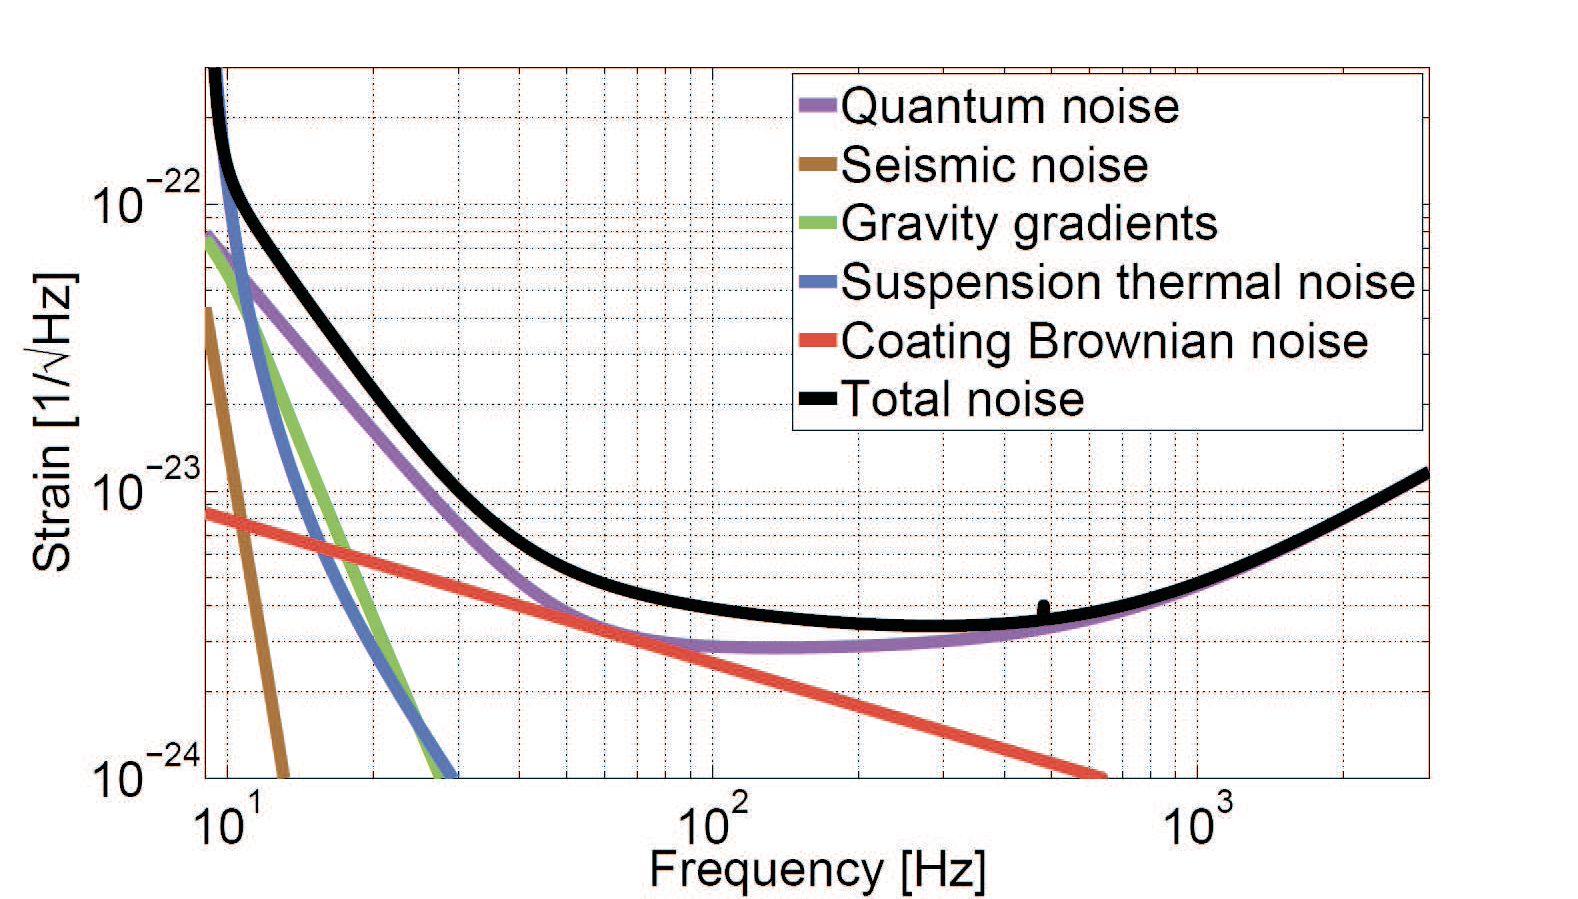
\includegraphics[width=\linewidth]{chapters/foundations/sections/cbc_searches/images/noise_limits_aligo.png}
		\caption{The noise budget of the advanced \acrshort{ligo} detectors.}\label{fig:noise_limit}
	\end{subfigure}
	\hspace{0.03\linewidth}
	\begin{subfigure}[b]{.34\linewidth}
		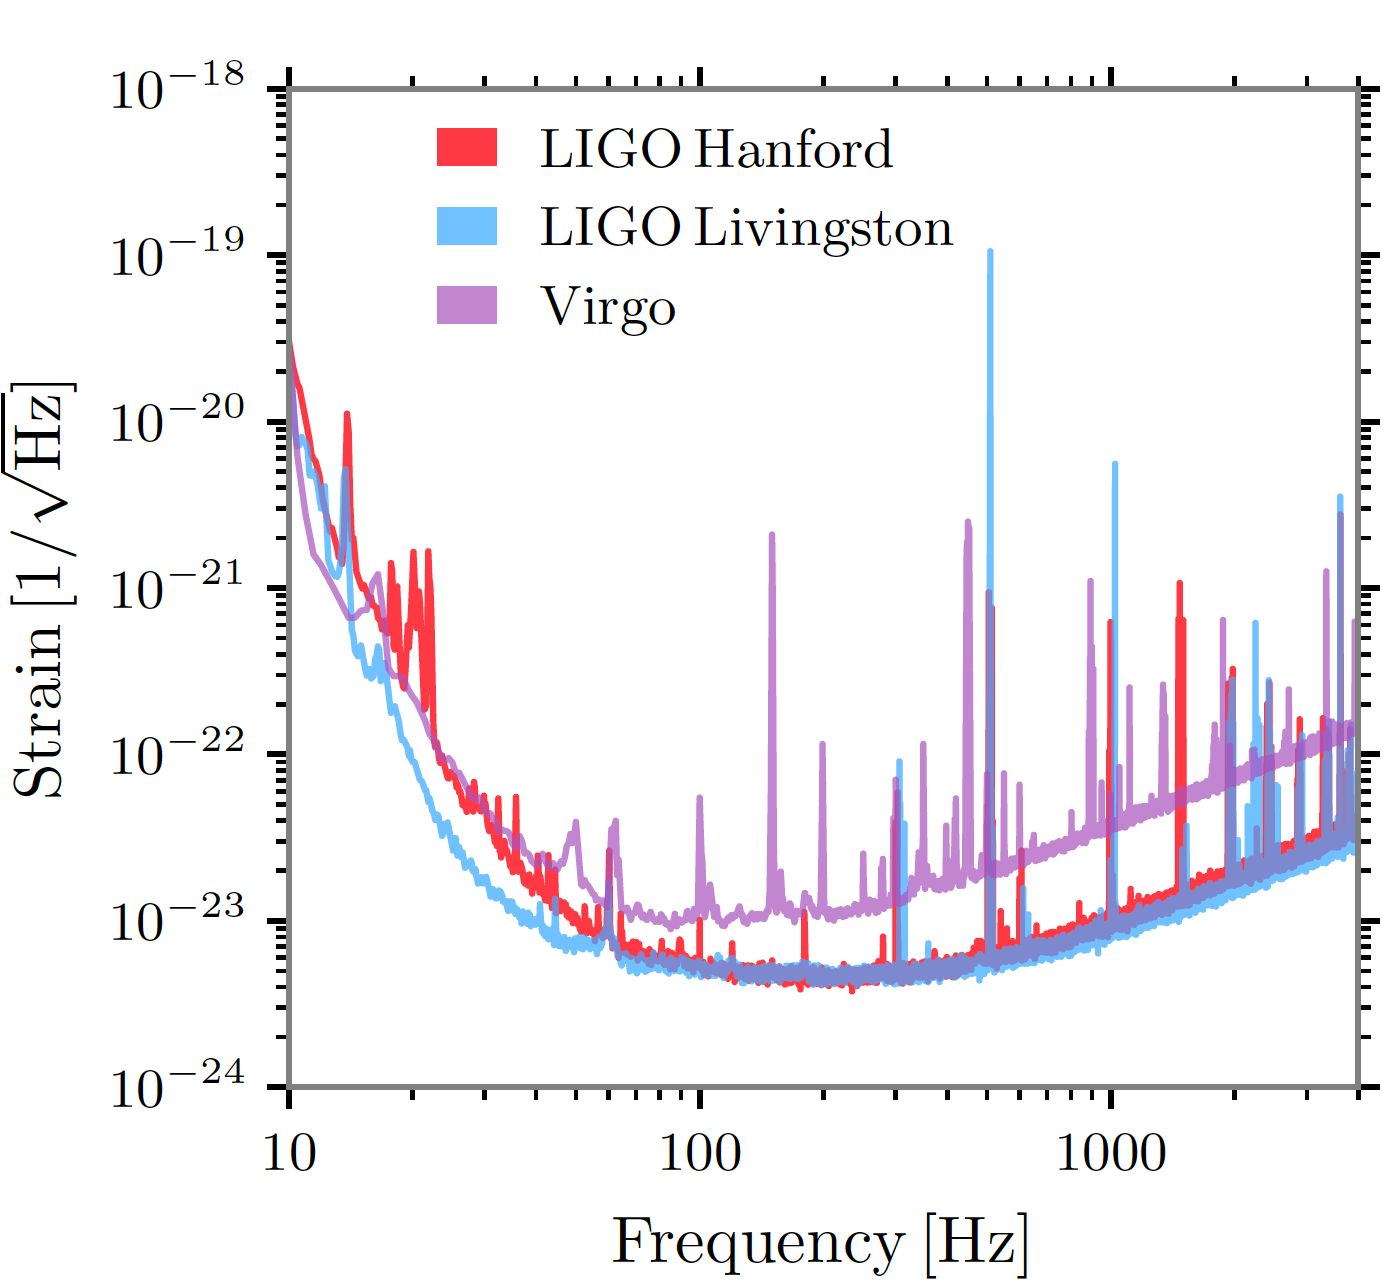
\includegraphics[width=\linewidth]{chapters/foundations/sections/cbc_searches/images/noise_o3_2.png}
		\caption{Power spectrum measured during \acrshort{o3}.}\label{fig:noise_o3}
	\end{subfigure}
	\caption[Noise amplitude spectrum]{The theoretical noise budget of the detector (a) and the measured amplitude spectrum (b) of advanced \acrshort{ligo}. The left figure shows the contribution of the different noise sources to the overall noise of the detector. It was taken from \cite{LIGOScientific:2014pky}. The right figure shows measured \acrshort{asd}s for the three main detectors during \acrshort{o3}. The curves are representative of the detector sensitivity during the observational period and the figure was taken from \cite{LIGOScientific:2021djp}.}
\end{figure}

To characterize the strength of the noise, one can calculate the \emph{power spectral density} (\acrshort{psd}). The \acrshort{psd} gives the power present in the detector due to noise as a function of the frequency. On a finite stretch of pure noise data $n\lr{t}$ with duration $T$ the one-sided \acrshort{psd} $S_n\lr{f}$ can be calculated as~\cite{Maggiore:2008aaa}%page 337
\begin{equation}
S_n\lr{f} = \frac{2}{T} \langle{\left|\tilde{n}\lr{f}\right|}^2\rangle,
\end{equation}
where $\tilde{n}\lr{f}$ is the Fourier transform of $n\lr{t}$ and the average $\langle\cdot\rangle$ is performed over different realizations of the noise. Its frequency resolution $\Delta f$ is given by $1/T$ and, by matching the units, one can infer that the \acrshort{psd} is given in units of \SI{}{1/\hertz}. In practice, the data is often chopped into many overlapping shorter pieces, a window is applied to each piece to reduce the impact of required periodicity of the Fourier transform, and the resulting \acrshort{psd}s are averaged. This algorithm is known as Welch's method~\cite{Welch:1967aaa}.

\autoref{fig:noise_o3} shows an estimate of the \emph{amplitude spectral density} (\acrshort{asd}) during the third observing run (\acrshort{o3}) for the three detectors that collected the majority of the data. The \acrshort{asd} is the square root of the \acrshort{psd}. Comparing it to the theoretical limit from \autoref{fig:noise_limit} one finds that the measured noise contains high spikes at certain frequencies. Most of these originate from known sources, such as the power grid frequency or violin modes of the mirror suspensions~\cite{LIGOScientific:2019hgc}. However, due to their narrow frequency range the effect on the detectability of \acrshort{gw}s from \acrshort{cbc} sources is marginal.

One noise characteristic that is not evident in the \acrshort{psd}s are short duration non-Gaussian noise transients known as \emph{glitches}. They can mimic the frequency evolution of real \acrshort{gw} events and a lot of effort is being invested to reject them \cite{Allen:1999yt, Allen:2004gu, Zevin:2016qwy, Robinet:2020lbf}. These glitches are by no means rare with an average glitch rate of \SIrange{0.29}{1.17}{\minute^{-1}}~\cite{LIGOScientific:2021djp}. The cause for some of these glitches is known and can be traced back for instance to light scattering or computer glitches; others have yet uncharacterized origins~\cite{Zevin:2016qwy}.

Several upgrades and extensions to the current network of ground based \acrshort{gw} detectors are planned. To extend the network in the short term future, it is planned to construct a third observatory of the advanced \acrshort{ligo} specifications in India~\cite{Iyer:2011aaa, Saleem:2021iwi}. It is scheduled to start operations around the year 2024~\cite{KAGRA:2013rdx}. The next major upgrades to the \acrshort{ligo} detectors are known as ``A+''. They are supposed to be incremental enhancements involving better light squeezing technology, bigger test masses, and improved materials, among other adjustments~\cite{LIGOScientific:2017aaa}. Beyond 2025 upgrades are still being planned but may include substantially increased laser power, a change of the laser frequency, and cryogenic operation~\cite{LIGOScientific:2017aaa}. One such proposal is named \acrshort{ligo} Voyager. Currently two new ground based detectors are being considered for constructions and are planned to become operational in the mid 2030s. These are the Einstein Telescope (\acrshort{et}) in Europe~\cite{Maggiore:2019uih} and Cosmic Explorer (\acrshort{ce}) in the United States~\cite{Reitze:2019iox}. \acrshort{et} is planned to be a triangular interferometric detector built underground. Its special shape allows to eliminate any signal from the data and be left with a pure noise channel. \acrshort{ce} plans to use an arm length of \SI{40}{\kilo\metre}.

To eliminate the low frequency limitations of earth bound observatories, two projects are developing space based detectors. The European Space Agency (\acrshort{esa}), the National Aeronautics and Space Administration (\acrshort{nasa}), and the \acrshort{lisa} Consortium are working on the Laser Interferometer Space Antenna (\acrshort{lisa})~\cite{LISA:2017pwj, ESA:2022aaa, NASA:2022aaa}. \acrshort{lisa} will be a constellation of three satellites on a heliocentric orbit following the earth. It will use time delay interferometry with an arm length of \SI{2.5}{\giga\metre} and is expected to detect \acrshort{gw}s in the sub-Hertz regime~\cite{LISA:2017pwj}. After a widely successful test of the technology known as \acrshort{lisa} Pathfinder~\cite{McNamara:2008zz, Armano:2016bkm, Armano:2018kix}, the \acrshort{lisa} mission is now scheduled to launch in 2034~\cite{ESA:2022aaa}. A second proposed space based observatory is the TianQin detector~\cite{TianQin:2015yph}. It, too, will consist of three satellites but its arm length is reduced to \SI[parse-numbers=false]{10^5}{\metre} and it will orbit the earth.

The final detection scheme I will briefly discuss are Pulsar Timing Arrays (\acrshort{pta})s~\cite{Hobbs:2008yn, Demorest:2009ex}. \acrshort{pta}s use the extreme timing accuracy of millisecond pulsars to measure large scale deviations of their arrival times over long periods. A \acrshort{gw} in the \SI{}{\nano\hertz} regime will cause these deviations to be correlated and be recoverable. They potentially allow to detect for instance the \acrshort{gw} background or other low frequency \acrshort{gw} sources. So far no signal consistent with expected \acrshort{gw}s has been recovered with high confidence~\cite{NANOGrav:2020gpb, NANOGrav:2020bcs}.


\subsection{Matched Filtering}\label{sec:matched_filtering}
As discussed in the previous subsection \ref{sec:detectors}, the output of the detectors is contaminated with large amounts of noise. To achieve optimal sensitivity, sophisticated data analysis techniques have to be used. This subsection will discuss a technique known as \emph{matched filtering}, that uses a model of the expected signal to maximize the amount of information that can be extracted from the data.

The output of the detector is a time series $d\lr{t}$ that is the sum of the noise $n\lr{t}$ and potentially an additive signal $h\lr{t}$
\begin{equation}
d\lr{t} = n\lr{t} + h\lr{t}.
\end{equation}
In the following discussion we will assume that the noise $n\lr{t}$ is stationary and Gaussian with zero mean. For real data this is only an approximation, as the noise characteristics slowly drift over time and glitches are short duration, non-Gaussian noise transients. However, the time scale of the noise drift is slow compared to the usual duration that \acrshort{cbc} signals are observable for~\cite{Kumar:2022tto}.

If one knows the signal that is hidden in the data, one can compare the data to the signal. To do so, one can convolve the expected signal, which is called the \emph{template}, with the data
\begin{align}\label{eq:concept_mf}
\lr{h\ast d}\lr{t} & = \int_{-\infty}^{\infty}\diff{\tau}\ h\lr{\tau}d\lr{t-\tau}\nonumber\\
& = \int_{-\infty}^{\infty}\diff{\tau}\ h\lr{\tau}h\lr{t-\tau} + \int_{-\infty}^{\infty}\diff{\tau}\ h\lr{\tau}n\lr{t-\tau}.
\end{align}
In this calculation, the first integral in the second line is positive definite when the template and the signal are aligned correctly, i.e. when $t=0$. Therefore, equation \eqref{eq:concept_mf} will yield larger values in the presence of the signal $h$ than in its absence. This is the core concept behind matched filtering.

\autoref{fig:detector_data_raw} shows a short time slice of data collected during \acrshort{ligo}s first observing run (\acrshort{o1}) and the \acrshort{asd} calculated from the detector data $d$ on a \SI{32}{\second} interval around the shown slice. The \acrshort{asd} shows that the detector noise is dominated by low frequencies, which becomes evident by the slow oscillations with large amplitudes in the left panel of \autoref{fig:detector_data_raw}. However, this also tells us that signals at low frequencies are much more likely to be overshadowed by noise. Therefore, one can downweigh frequencies where the detector is particularly noisy.

\begin{figure}
	\centering
	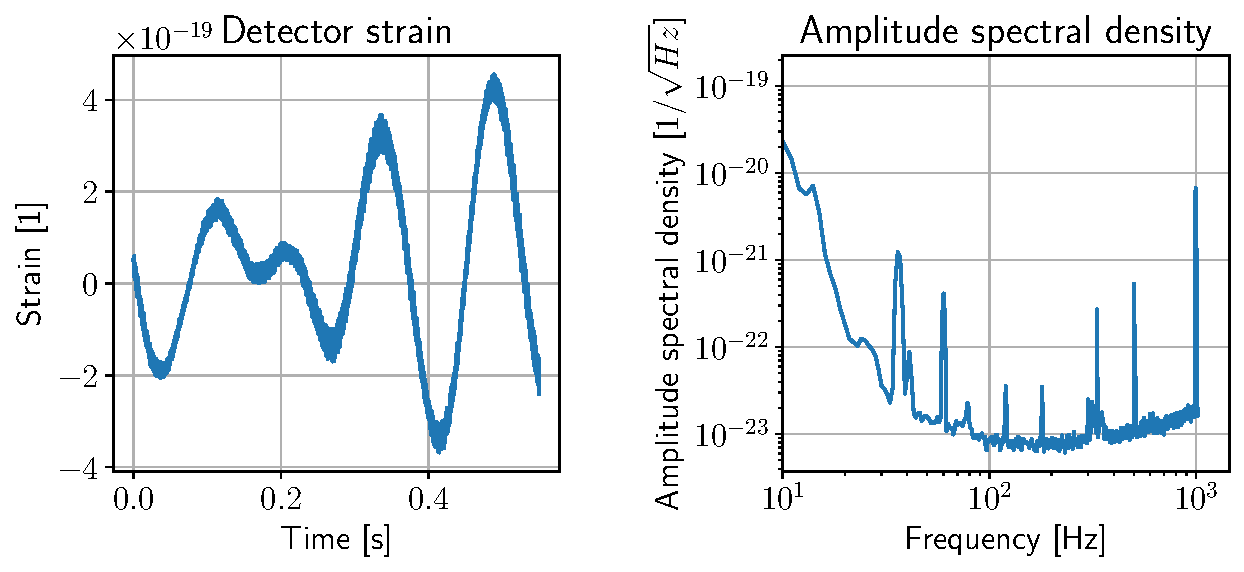
\includegraphics[width=0.98\textwidth]{chapters/foundations/sections/cbc_searches/images/data_raw.pdf}
	\caption[Raw detector data]{A small slice of raw detector data from the Gravitational Wave Open Science Center (\acrshort{gwosc}) (left) and the corresponding \acrshort{asd} (right). The \acrshort{asd} was calculated from \SI{32}{\second} around the shown data slice using Welch's method with a window duration of \SI{1}{\second} and a step size of \SI{0.5}{\second} between the windows~\cite{LIGOScientific:2019lzm}.}\label{fig:detector_data_raw}
\end{figure}

In practice this process is called \emph{whitening}, as it attempts to scale the power at each frequency to be $1$. Noise which has a flat \acrshort{psd} is known as white noise. This can be achieved by dividing the Fourier transformed data $\tilde{d}\lr{f}$ by the \acrshort{asd}
\begin{equation}
\hat{d}\lr{t} = \int \diff{f}\ \frac{\tilde{d}\lr{f}}{\sqrt{S_n\lr{f}}} e^{i2\pi ft}.
\end{equation}
This operation in the time domain is a convolution of the data $d$ with a filter $F^{-1}\lr{1/\sqrt{S_n\lr{f}}}$, where the function $F^{-1}$ represents the inverse Fourier transform. Due to high peaks in the \acrshort{asd} at some frequencies, the filter has non-negligible power even at times far away from zero. Since the Fourier transform assumes the data to be periodic, the long duration of the filter correlates independent data points and corrupts the data. To avoid this corruption the filter is truncated in the time domain to a finite duration, by applying a window that tapers to zero. The corruption is, thereby, limited to half the truncated duration of the filter in the beginning and end of the whitened data. The corrupted parts of the data are subsequently cropped. By truncating the whitening filter in the time domain, the sharp frequency lines of the \acrshort{asd} are broadened which is usually not a problem for \acrshort{cbc} signal detection.

\autoref{fig:detector_data_white} shows the same data as \autoref{fig:detector_data_raw} but with whitening applied to it. The \acrshort{asd} is now almost flat and has a value of $\approx 1$ at each frequency. Looking closely, one can start to make out a waveform around \SI{0.4}{\second} from the start of the data. Cropping to remove edge effects was applied outside of the shown window.

\begin{figure}
	\centering
	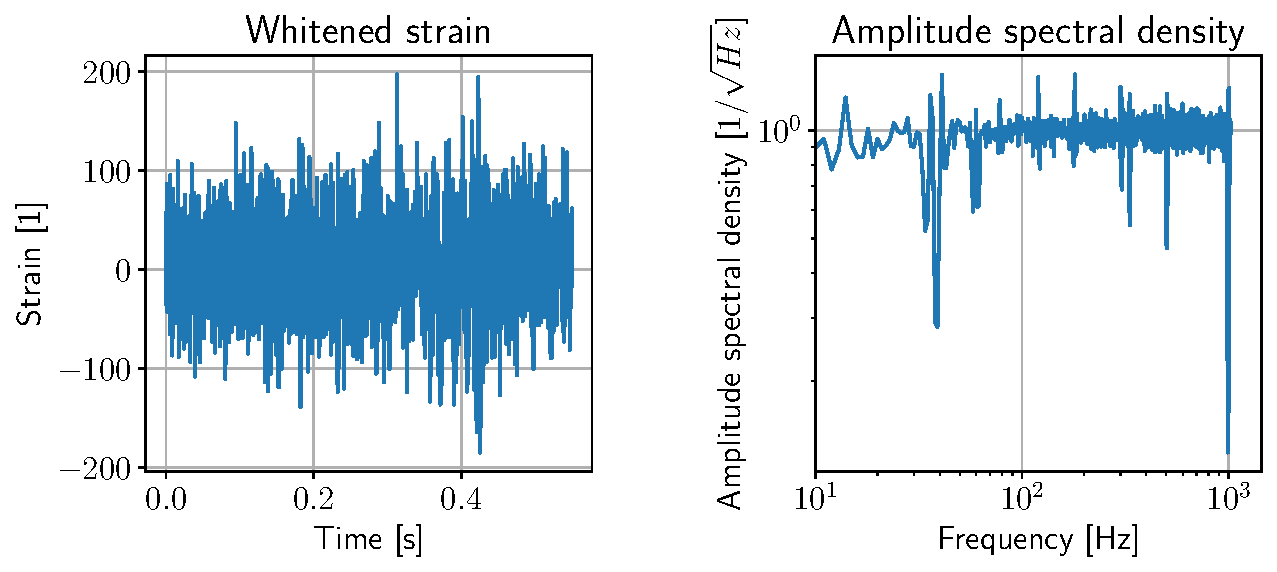
\includegraphics[width=0.98\textwidth]{chapters/foundations/sections/cbc_searches/images/data_white.pdf}
	\caption[Whitened detector data]{The data shown in \autoref{fig:detector_data_raw} whitened by the associated \acrshort{psd} (left) and the \acrshort{asd} calculated on the whitened data (right). The entire \SI{32}{\second} of data were whitened. Therefore, edge effects are clipped from the shown data slice.}\label{fig:detector_data_white}
\end{figure}

Using the whitened data and an accordingly whitened template in \eqref{eq:concept_mf} maximizes the difference between the value obtained when filtering pure noise and noise with the template added into it~\cite{Maggiore:2008aaa}. It is mathematically proven to be the optimal filter for stationary Gaussian noise~\cite{Allen:2005fk}. Since the data and template are transformed to the Fourier domain to whiten them and since the convolution operation can be expressed by a multiplication in the Fourier domain, the matched filter is given by~\cite{Maggiore:2008aaa, Usman:2015kfa}% page 345
\begin{equation}
\rho\lr{t} = \frac{\langle h\vert d\rangle}{\sqrt{\langle h\vert h\rangle}},
\end{equation}
where
\begin{equation}\label{eq:mf_inner_product}
\langle a\vert b\rangle\lr{t} = 4\text{Re}\left[\int_0^\infty\diff{f}\ \frac{\tilde{a}^\ast\lr{f}\tilde{b}\lr{f}}{S_n\lr{f}} e^{i2\pi ft}\right].
\end{equation}
The factor $\sqrt{\langle h\vert h\rangle}$ is used for normalization and the factor $4$ comes from using the one-sided \acrshort{psd} as well as taking the integral of the symmetric argument from $0$ instead of $-\infty$. The function $\text{Re}\left[\cdot\right]$ extracts the real part of a complex number. The function $\rho\lr{t}$ is the \emph{signal-to-noise ratio} (\acrshort{snr}). When the \acrshort{snr} exceeds a threshold, which is determined by search configurations, the search has potentially identified the signal.

So far it was assumed that the signal in the data is known. In reality this assumption does not hold, as we do not even know if a signal is present and if one is present, what kind of system emitted it. However, matched filtering is highly sensitive to the phase of the signal. This means that when the phases of the template and the actual signal deviate by even a moderate amount, the \acrshort{snr} drops significantly. For this reason, one usually constructs a \emph{template bank}, that covers a specified region of possible parameters. It is constructed by requiring that the \emph{match} between two neighboring templates does not fall below a given limit. The match is the inner product \eqref{eq:mf_inner_product} of the two signals, maximized over the phase and coalescence time, and normalized by the norm induced by the inner product \eqref{eq:mf_inner_product} of both templates. Usually matches $\geq 0.95$ are required~\cite{LIGOScientific:2021djp, Nitz:2021uxj}.

The data has to be filtered against every template in the bank. Therefore, the computational cost scales linearly with the number of templates. However, the number of templates scales exponentially with the number of degrees of freedom in the system. For this reason, it is desirable to reduce the dimensions of the parameter space as much as possible. To do so, searches make a series of assumptions and optimizations. First, search template banks are usually constructed using only the dominant $22$-mode. This means that equation \eqref{eq:complex_waveform} essentially reduces to
\begin{equation}
H = h_+ + i h_\times = A\lr{\tau, r, \iota, \Phi_0, \kappa} e^{-i\Phi\lr{\tau, \kappa}}.
\end{equation}
Second, by using
\begin{equation}
h_+ = \frac{H + H^\ast}{2},\ \quad
h_\times = \frac{H - H^\ast}{2i}
\end{equation}
in \eqref{eq:delta_l} one finds that the measured strain in the detector is of the form~\cite{Allen:2005fk}
\begin{equation}\label{eq:qualitativ_detector_output}
h = \text{Re}\left[\frac{A\lr{\tau, \kappa}}{D_\text{eff}\lr{r, \theta, \phi, \psi, \iota}}\exp\lr{-i\lr{2\Delta\Phi\lr{\theta, \phi, \psi, \iota, \Phi_0} + 2\Phi\lr{\tau, \kappa}}}\right].
\end{equation}
$D_\text{eff}$ is known as the effective distance and quotes the distance at which the same source could be seen with the same amplitude, assuming an optimal orientation and a location directly overhead the detector. An explicit expression for $D_\text{eff}$ can be found in \cite{Allen:2005fk}. $\kappa$ represents all source internal parameters, i.e. the masses, spins, and tidal deformabilities. From \eqref{eq:qualitativ_detector_output} we find that the source location and orientation with respect to the detector introduce a time independent phase shift and scale the amplitude. The amplitude scaling can be combined with the distance $r$ to form a single parameter; the effective distance. Observing a source in one location has the same amplitude evolution as observing the same source at the optimal location and orientation, just at a farther distance. The phase shift on the other hand can be combined with the coalescence phase, to form a second effective parameter. So instead of being concerned with the $4$ parameters $\theta$, $\phi$, $\psi$, and $\iota$, all of them can be absorbed into the distance $r$ and coalescence phase $\Phi_0$. The distance, on the other hand, sets a normalized scale for the \acrshort{snr} and, therefore, does not need to be included in the template bank~\cite{Allen:2005fk}. The coalescence phase can also be eliminated from the template bank, by maximizing the \acrshort{snr} over it. If the projection onto the real axis in \eqref{eq:mf_inner_product} is removed, the \acrshort{snr} time series becomes complex. An overall phase shift in the template rotates the \acrshort{snr}-vector in the complex plane, but does not change its length. So by taking the absolute value of the \acrshort{snr} time series, one maximizes its value over the coalescence phase, irrespective of the phase value. This is equivalent to using the total \acrshort{snr} by combining the \acrshort{snr} of filtering with the template $h$ and its phase shifted counterpart $ih$~\cite{Allen:2005fk, Ohme:2012cba, Usman:2015kfa}
\begin{equation}
\rho_{\Phi_{0,\text{max}}}\lr{t} = \sqrt{\frac{{\langle h\vert d\rangle}^2+{\langle ih\vert d\rangle}^2}{\langle h\vert h\rangle}}.
\end{equation}

Third, template banks usually assume non-precessing systems~\cite{LIGOScientific:2021djp, Nitz:2021zwj}. This reduces the dimensionality of the parameter space even further, as the original $6$ spin parameters are reduced to a total of $2$ values that need to be covered. Finally, the inverse Fourier transform in \eqref{eq:mf_inner_product} is equivalent to doing a convolution of the data with a template. So it efficiently changes the coalescence time $t_0$ of the template and produces the \acrshort{snr} value for all possible values. All these optimizations lead to a four dimensional space that needs to be covered by the template bank; $m_1$, $m_2$, $\chi_1^3$, $\chi_2^3$.

Current standard searches are limited to systems with aligned spin and a mass range from $\approx$ \SI{1}{M_\odot} to $\approx$ \SI{500}{M_\odot}, depending on the implementation~\cite{LIGOScientific:2021djp, Nitz:2021uxj}. Lower masses require denser template banks, as the systems are within the sensitive band of the detectors for a larger number of cycles. This allows small phase errors to accumulate to the point where match requirements are exceeded~\cite{Harry:2009ea}. The high-mass region is rather limited by the short duration, which makes it difficult to distinguish astrophysical signals from glitches~\cite{Nitz:2017lco}.

Although using matched filtering alone is sufficient to detect \acrshort{gw}s, it is often stated that the first detected \acrshort{gw} is visible in the data with the naked eye. While one can barely make something out in \autoref{fig:detector_data_white}, we can make use of the fact that we know the frequencies of the signal. \autoref{fig:detector_data_bandpassed} shows the data after whitening and applying an additional bandpass filter for the range \SIrange{20}{256}{\hertz}. The signal is now clearly visible in the time domain data.

\begin{figure}
	\centering
	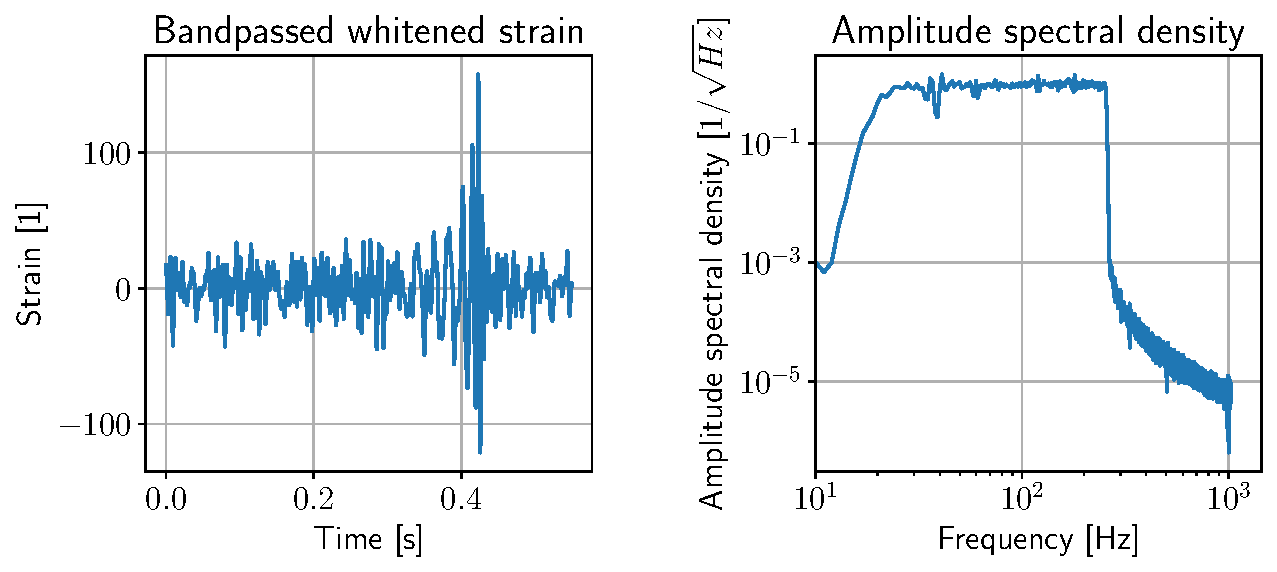
\includegraphics[width=0.98\textwidth]{chapters/foundations/sections/cbc_searches/images/data_bandpassed.pdf}
	\caption[Bandpassed and whitened detector data]{The whitened data from \autoref{fig:detector_data_white} with a highpass filter of \SI{20}{\hertz} and a lowpass filter of \SI{256}{\hertz} applied (left). The corresponding \acrshort{asd} is shown on the right. The signal is now clearly visible. The data for all of these figures is the Hanford data around GW150914~\cite{LIGOScientific:2016aoc}.}\label{fig:detector_data_bandpassed}
\end{figure}

Since matched filtering is mathematically proven to be the optimal descriminator between pure noise and noise plus signal~\cite{Allen:2005fk}, it is used as a target for the deep learning detection algorithms discussed in this thesis.

This section discussed detection algorithms based on matched filtering. Due to heavy optimization, these algorithms are not designed to make statements about many of the interesting parameters of the source. The task of extracting all parameters that influence the waveform from the data is called \emph{parameter estimation}. These algorithms explore the likelihood surface and allow to give estimates of the parameters of the source and quantify them with error bars. Since the likelihood usually has to be estimated for millions of points, these algorithms are computationally very expensive and can take days or even weeks to converge. For a deeper explanation see for instance \cite{LIGOScientific:2016vlm, Biwer:2018osg, LIGOScientific:2019hgc}.


\subsection{Search Algorithm and Significance of Detections}
The matched filter of the previous subsection produces a \acrshort{snr} time series for every template. These are numerical values where larger values usually imply a greater certainty that a \acrshort{gw} is present in the data. Values of this kind are known as \emph{ranking statistic}. The question a detection pipeline has to answer is: What value of the ranking statistic is required for us to be confident that we have detected a \acrshort{gw}? This subsection will go into how this question is answered. I will follow the order of steps used by the PyCBC offline analysis~\cite{Usman:2015kfa} but note that other modeled pipelines conceptually work the same way and only differ in details~\cite{Messick:2016aqy, Adams:2015ulm}.

The first step a search pipeline has to perform is to select the data that should be analyzed. The noise characteristics of the detectors change over time~\cite{LIGOScientific:2019hgc}. During some periods, the data quality drops to a level where analysis would lead to excessive rates of false positive detections. For this reason, these parts of the data are identified by high-level quality checks~\cite{LIGO:2021ppb} and excised from the analysis data. Easily identifiable loud glitches are also cropped from the data~\cite{LIGO:2021ppb}. The overall shape of the stationary component of the noise is estimated by calculating the average \acrshort{psd} for each detector and an appropriate template bank is constructed~\cite{Usman:2015kfa}.

Afterward, the data from all detectors are filtered against the template bank to produce \acrshort{snr} time series. From there, candidate events are identified by applying a simple threshold to the \acrshort{snr} time series. The resulting points are subsequently clustered for each template, as especially loud signals usually exceed the threshold for multiple samples. The cluster window duration is a free parameter, which has to be small compared to the expected time between signals and subsequent glitches.

If the noise in the detector were stationary and purely Gaussian, one could take the \acrshort{snr} values of the candidate events as a ranking statistic. However, as discussed in subsection \ref{sec:detectors} the noise is frequently contaminated with glitches. Those that have not been removed from the data can lead to large \acrshort{snr} values, even when the underlying process that produced the transient has little to no resemblance to the signal one is searching for. Therefore, the \acrshort{snr} is usually augmented with additional statistics to form the ranking statistic. The goal of these additional statistics is to reduce the value of the ranking statistic for glitches, i.e. down weighting their influence.

The most common adaptation is to to check the data for consistency with the template. PyCBC and MBTA use a $\chi^2$-test that checks if the evolution of the potential signal matches the expected signal evolution in different time- and frequency-bands~\cite{Allen:2004gu, Usman:2015kfa, Adams:2015ulm}. GstLAL uses a $\xi^2$-test that checks the evolution of the \acrshort{snr} time series against the expected evolution~\cite{Messick:2016aqy}. More recently, efforts were made to include the short term fluctuations of the \acrshort{psd} into the ranking statistic~\cite{Venumadhav:2019tad, Nitz:2020oeq}. This reduces the impact of a less stationary detector on the trigger rate.

Once the triggers and their corresponding ranking statistics have been determined for each detector individually, they are checked for coincidences between multiple observatories. A signal from an astrophysical source has to be present in all detectors and arrival times may not differ by more than the time of flight difference between the detectors. Additionally, coincident triggers must be generated from the same template and the amplitude and phase evolution must be consistent with the time delay between the detectors~\cite{Nitz:2017svb}. These criteria already eliminate many false detections caused by glitches or other noise processes. For surviving triggers, the single detector ranking statistics are combined into a coincident ranking statistic. In recent works the coincident ranking statistic was further altered by incorporating information on the expected noise and signal trigger rates for different source parameters~\cite{Nitz:2017svb}.

As a final step, the search algorithm has to relate the numerical value of the coincident ranking statistic to a measure of how confident we are to have detected a \acrshort{gw}. In other words, the analysis must check how often a false detection is made at a given ranking statistic value. The number of false positive detections per unit time is known as the \emph{false-alarm rate} (\acrshort{far}). It is estimated by analyzing constructed background data. The background data is constructed by time shifting the single detector triggers of one detector by a duration longer than the time of flight difference between the detectors. This way, any coincident trigger cannot be of astrophysical origin. By applying multiple different time shifts, the theoretical amount of data which can only contain false positives can be extended to millions of years~\cite{Usman:2015kfa}. To determine the \acrshort{far} at a ranking statistic, the number of false positives with a coincident ranking statistic larger than the threshold are counted and divided by the theoretical duration of the analyzed data:
\begin{equation}
\mathcal{F}_\rho = \frac{N_\rho}{T}.
\end{equation}
Here $\mathcal{F}_\rho$ is the \acrshort{far} for the coincident ranking statistic $\rho$, $N_\rho$ is the number of false positives in the background with a ranking statistic $\geq\rho$, and $T$ is the duration of the analyzed background.

This thesis is mainly concerned with the comparison of machine learning based search algorithms against matched-filter based searches. For this comparison, one can analyze a simulated population of sources with both algorithms and study how many signals are recovered by either search. However, for a fair comparison we want to assess the sensitivities at the same useful astrophysical \acrshort{far}. Furthermore, to allow for an objective comparison between different works, the sensitivity must be normalized to the population. In the extreme case, the number of detected sources can always be driven to zero by choosing a population of signals injected into the noise where all sources are excessively far away. For these reasons, all works discussed in this thesis estimate the sensitive distance of the search for sensible populations. I will briefly introduce it here.

Let $\Phi\lr{\vec{x}, \lambda}$ be the probability distribution that describes the injected population, where $\vec{x}$ is the location in space and $\lambda$ are the remaining source parameters. Let, further, $\epsilon\lr{\vec{x}, \lambda; \mathcal{F}}$ be the fraction of injections being recovered by the search with parameters $\vec{x}$ and $\lambda$ with \acrshort{far} $\leq\mathcal{F}$. Then the expectation value of the volume from which sources are detected is given by~\cite{Usman:2015kfa}
\begin{equation}
\langle V\lr{\mathcal{F}}\rangle = \int \Diff{3}{x}\diff{\lambda}\ \frac{\Diff{3}{V\lr{\vec{x}}}}{{\diff x}^3}\Phi\lr{\vec{x}, \lambda}\epsilon\lr{\vec{x}, \lambda; \mathcal{F}},
\end{equation}
where $\frac{\Diff{3}{V\lr{\vec{x}}}}{{\diff x}^3}$ is the differential volume element. This volume is usually measured empirically, by applying the search to data with many known injections drawn from the distribution $\Phi$. The integral can then be estimated by Monte-Carlo integration. If the prior is uniform in volume, the sensitive volume is proportional to counting the recovered injections. This counting statistic then needs to be normalized to the prior volume and the number of injections. If the prior volume is a sphere with radius $r_\text{max}$ where injections are distributed uniformly in volume, the Monte-Carlo approximation of the sensitive volume is given by~\cite{Usman:2015kfa}
\begin{equation}
\langle V\lr{\mathcal{F}}\rangle\approx V\lr{r_\text{max}}\frac{N_{I, \mathcal{F}}}{N_I},
\end{equation}
where $N_{I, \mathcal{F}}$ is the number of injections recovered from the data with \acrshort{far} $\leq \mathcal{F}$, $N_I$ is the total number of injections in the data, and $V\lr{r_\text{max}}$ is the volume of a sphere with radius $r_\text{max}$. When a different distribution is used to sample the injections, the formula has to be reweighted or the integral has to be computed. The sensitive distance is defined as the radius of a sphere with volume $\langle V\lr{\mathcal{F}}\rangle$. As such, it is the average distance from which the search can detect sources and not an upper limit.

\section{Deep Learning}\label{sec:deep_learning}
\acrfull{ai}, \acrfull{ml}, and deep learning are terms often used interchangeably and to describe a wide range of topics. The beginning of this section tries to clarify the meaning of these terms in the context of this work before discussing the topic of deep learning in more detail.

\acrshort{ai} is the broadest of the three topics and encompasses the others~\cite{Goodfellow:2016:DNN}. 
%Fig 1.4
While it lacks an agreed-upon definition, the term broadly describes the research dedicated to creating machines that enact some form of intelligence \cite{nilsson:2009}. However, this only shifts the burden of definition to the term ``intelligence''. In his excellent book on the history of \acrshort{ai} Nilsson describes intelligence as the ``quality that enables an entity to function appropriately and with foresight in its environment'' \cite{nilsson:2009}. Taking these definitions as a basis, \acrshort{ai} research tries to create algorithms or machines that make decisions based on their environment to maximize their chance of success to achieve some goal.

\acrshort{ml} is part of the research field on \acrshort{ai} and aims to create algorithms that extract general features from example data. These learned features are then to be used to make predictions about samples that were not part of the example data. It specifically requires algorithms to improve based on past experiences~\cite{Goodfellow:2016:DNN}. 
%page 1
Usually, a general purpose framework is adapted to specific problems only through a prior training phase, where the algorithm is exposed to example data. This means that the learning algorithm does not have to be changed to adapt to different data.

An example for a class of \acrshort{ai} algorithms that do not fall under the category of \acrshort{ml} algorithms are knowledge based approaches. These try to encode knowledge in a formal language and infer decisions by querying the resulting database.~\cite{Goodfellow:2016:DNN}. 
%page 2
The Cyc project is one of the most well known approaches to a knowledge based \acrshort{ai} and makes use of the CycL language~\cite{Lenat:1989aaa}. However, creating a database that is both suitably large and complex is very labor intensive and often more fragile than utilizing \acrshort{ml} algorithms. For these reasons \acrshort{ml} is currently the most widespread approach to \acrshort{ai}.

Deep learning refers to \acrshort{ml} algorithms which utilize a specific kind of framework; deep neural networks (\acrshort{nn}s). While the concept of \acrshort{nn}s will be introduced in detail below, in short they are directed graphs that apply simple functions at every node, where the weights of the edges are optimized during the training phase based on the example data. These graphs can be structured into layers and a \acrshort{nn} is called deep, when the network is composed of many subsequent layers~\cite{Goodfellow:2016:DNN}.

Besides deep learning, there are many other kinds of \acrshort{ml} algorithms. Some examples include random forests~\cite{Ho:1995aaa}, support vector machines (\acrshort{svm}s) \cite{Boser:1992aaa}, and Gaussian process regression. Even simple regression algorithms, like linear regression, can be seen as a kind of \acrshort{ml} algorithms~\cite{Geron:2017aaa}. 
%page XV
For a short overview of these different types see for instance chapter 1 and for a more detailed discussion chapters 5 to 7 of \cite{Geron:2017aaa}.

All \acrshort{ml} algorithms can broadly be classified into three categories based on the~\emph{training} mechanism, where training is the process of improving the algorithm based on example data. These three classes are \emph{supervised learning}, \emph{unsupervised learning}, and \emph{reinforcement learning}~\cite{Goodfellow:2016:DNN, Ghahramani:2004}. In supervised learning tasks the desired output $y$ -- often called \emph{label} or \emph{target} -- for example data $x$ is known~\cite{Geron:2017aaa} and the algorithm tries to approximate the conditional probability distribution $p\lr{y \given x}$~\cite{Goodfellow:2016:DNN}. 
%page 8 and page 103
Regression algorithms are a good example for supervised learning. In unsupervised learning only the example data $x$ is known and the \acrshort{ml} algorithm is tasked with finding the underlying probability distribution $p\lr{x}$~\cite{Goodfellow:2016:DNN}. 
%page 103
Many clustering algorithms are a prime example for unsupervised learning. Reinforcement learning is completely detached from the previous two classes. Here the algorithm observes the state of its environment and has to decide on an action it wants to take. It is then rewarded or penalized based on the action it has chosen~\cite{Geron:2017aaa,sutton:2018}. 
%page 8
The algorithm learns by trial and error, without human intervention. This kind of learning is especially popular in the field of robotics and computer games~\cite{Goodfellow:2016:DNN,Finn:2015aaa,Sallab:2017,Mnih:2015aaa,openai:2019}.
%page 25
The above mentioned classifications of algorithms are by no means rigid. A single algorithm may also be trained by a combination of the above mentioned strategies. There are also other means of classifying \acrshort{ml} algorithms into different categories~\cite{Geron:2017aaa}.
%page 8

Today \acrshort{ml} algorithms are used anywhere from recommendation systems in the entertainment industry~\cite{Steck:2021aaa} to advanced medical diagnostics~\cite{Esteva:2019aaa}. Especially \acrshort{nn}s have gained a lot of traction in recent years and improved state-of-the-art performance for \acrshort{ml} algorithms for a wide variety of tasks such as image recognition \cite{krizhevsky:2012, Szegedy:2015, Russakovsky:2015aaa}, autonomous driving \cite{Sallab:2017}, playing board- \cite{Silver:2016} and computer-games \cite{openai:2019}, speech recognition \cite{Hinton:2012}, or audio synthesis \cite{Oord:2016wav}. \acrshort{ml} algorithms have also been applied in many scientific fields~\cite{Deiana:2021niw}, some of which are the prediction of protein structure used in pharmaceutical studies~\cite{Alquraishi:2021aaa, Jumper:2021aaa}, improvements to material composition and synthesis~\cite{Butler:2018aaa}, and event reconstruction at the Large Hadron Collider~\cite{Gray:2020mcm}. Machine learning has also been explored as an option for many tasks in \acrshort{gw} data analysis and \acrshort{gw} astronomy and an overview is given in \autoref{sec:ml-gw-hist}.

This work considers only neural networks as a means of machine learning. For this reason the basic concepts as well as a few advanced techniques will be briefly introduced in the following subsections. For a more thorough introduction I recommend \cite{Goodfellow:2016:DNN} for a deep dive into the topic, \cite{Geron:2017aaa} for a more applied approach, and \cite{Nielsen:2015:DNN} for a quick and easy to understand overview.

\subsection{Neural Networks}\label{sec:nn}
The start of the research on neural networks based on the theory of computation and mathematics can be traced back to a study conducted by McCulloch and Pitts in 1943~\cite{McCulloch:1943}. They tried to come up with a model description of the human brain, where they modeled neurons by utilizing propositional logic. By making the simplifying assumptions that neurons have an arbitrary number of binary inputs, a single binary output that is one (i.e. ``fires'') only if a pre-defined number of inputs is active, and that individual inputs may prevent any output, they were able to build all logic gates and combine them to do complex computations~\cite{Piccinini:2004}. While the original work exclusively used propositional logic, their idea of the neuron can suggestively be expressed by the functional form
\begin{equation}\label{eq:neuron-pitts}
n: {\left\{0,1\right\}}^m\times{\left\{-1,1\right\}}^m\times\mathbb{Z} \to\left\{0,1\right\};\ \lr{\vec{x}, \vec{w}, b} \mapsto H\lr{\vec{x}\cdot\vec{w} + b},
\end{equation}
where $\vec{x}$ are the inputs to the neuron, $\vec{w}$ are known as the weights, $b$ is known as the bias, ans $H$ is the Heaviside function. See \autoref{fig:heavyside_neuron} for a depiction. This definition of the neuron is not equivalent to the idea proposed by McCulloch and Pitts but conveys the central findings of their study and leads to a more coherent picture of subsequent developments.

\begin{figure}
	\centering
	\begin{tikzpicture}[
neuron/.style={minimum size=0.75cm, circle, draw},
heavyside/.style={path picture={
	\pgfpointdiff{\pgfpointanchor{path picture bounding box}{north east}}%
        {\pgfpointanchor{path picture bounding box}{south west}}
      \pgfgetlastxy\x\y
      % Scale the x and y vectors so that the range
      % -1 to 1 is slightly shorter than the size of the node
      \tikzset{x=\x*.25, y=\y*.25}
	\draw (-1,-1) -- (0, -1) -- (0, 1) -- (1, 1);
}}
]

\node[neuron, heavyside] (n) {};

\node (z) [below=0.1cm of n] {$z = \vec{w}\cdot\vec{x}+b$};
\node (x_1) [left=1.5cm of n] {$x_1$};
\node (x_0) [above=0.5cm of x_1] {$x_0$};
\node (x_2) [below=0.5cm of x_1] {$x_2$};
\node (a) [right=1.5cm of n] {$H\lr{z}$};

\draw[->, shorten >= 2pt] (x_0) -- (n) node[midway, above] {$w_0$};
\draw[->, shorten >= 2pt] (x_1) -- (n) node[midway, above] {$w_1$};
\draw[->, shorten >= 2pt] (x_2) -- (n) node[midway, above] {$w_2$};

\draw[->, shorten >= 2pt] (n) -- (a);

\end{tikzpicture}
	\caption[McCulloch-Pitts-neuron]{Depiction of the neuron defined in \eqref{eq:neuron-pitts}. The inputs $x_0, x_1, x_2$ are either $0$ or $1$. The weights $w_0, w_1, w_2$ are either $-1$ or $1$. The bias $b$ is a whole number. $H$ is the Heaviside function.}\label{fig:heavyside_neuron}
\end{figure}

To form basic logic gates, values for the parameters $\vec{w}$ and $b$ have to be chosen. The ''and''-operation $A\land B$ is obtained by setting $\vec{w}=\lr{1, 1}^T,\ b=-1$, whereas the ''not''-operation $\neg A$ can be represented by $w=-1,\ b=1$. These simple gates can then be connected to form complex computational graphs and compute any computable function. However, notice that the parameters of these networks have to be hand-picked.

In 1957 Rosenblatt introduced the Perceptron~\cite{rosenblatt:1958}. Instead of restricting individual neurons to have binary inputs and discrete weights, he allowed all arguments to be real numbers
\begin{equation}\label{eq:neuron-rosenblatt}
n: \R^m\times \R^m\times \R \to \left\{0,1\right\};\ \lr{\vec{x}, \vec{w}, b}\mapsto H\lr{\vec{w}\cdot\vec{x} + b}.
\end{equation}
More importantly, however, he proposed an algorithm based on the Hebbian principal that allowed the parameters of the network to be optimized from example data. The Hebbian principal states that directly connected neurons that often fire together form stronger bonds; ''Neurons that fire together, wire together.''~\cite{Geron:2017aaa} The Perceptron is a collection of these neurons, where every neuron is connected to all inputs. The number of binary outputs, therefore, is equivalent to the number of neurons in the Perceptron. The left panel of \autoref{fig:mlp} shows an example of a perceptron. 

\begin{figure}
	\centering
	\begin{tikzpicture}[
neuron/.style={minimum size=0.75cm, circle, draw},
heavyside/.style={path picture={
	\pgfpointdiff{\pgfpointanchor{path picture bounding box}{north east}}%
        {\pgfpointanchor{path picture bounding box}{south west}}
      \pgfgetlastxy\x\y
      % Scale the x and y vectors so that the range
      % -1 to 1 is slightly shorter than the size of the node
      \tikzset{x=\x*.25, y=\y*.25}
	\draw (-1,-1) -- (0, -1) -- (0, 1) -- (1, 1);
}}
]
\begin{scope}[on grid,node distance=0.5cm]
	% PERCEPTRON
	% Inputs of Perceptron
	\node (x_0) {$x_0$};
	\node (x_1) [below=1cm of x_0] {$x_1$};
	
	% Nodes of Perceptron
	\node[neuron, heavyside] (mlp10) [above right=0.5cm and 1.5cm of x_0] {};
	\node[neuron, heavyside] (mlp11) [below right=0.5cm and 1.5cm of x_0] {};
	\node[neuron, heavyside] (mlp12) [below right=0.5cm and 1.5cm of x_1] {};
	
	% Connections of Perceptron
	\draw[->, shorten >= 2pt] (x_0.east) -- (mlp10);
	\draw[->, shorten >= 2pt] (x_0.east) -- (mlp11);
	\draw[->, shorten >= 2pt] (x_0.east) -- (mlp12);
	
	\draw[->, shorten >= 2pt] (x_1.east) -- (mlp10);
	\draw[->, shorten >= 2pt] (x_1.east) -- (mlp11);
	\draw[->, shorten >= 2pt] (x_1.east) -- (mlp12);
	
	
	% Splitting figure
	\node (a) [above left=0.5cm and 0.5cm of x_0] {(a)};

	\node (ht) [above right=0.25cm and 1cm of mlp10] {};
	\node (hb) [below right=0.25cm and 1cm of mlp12] {};
	
	%\draw[] (ht) -- (hb);
	
	\node (helper1) [right=1cm of ht] {};
	\node (b) at (a -| helper1) {(b)};
	
	
	% MLP
	% Inputs of MLP
	\node (helper2) [right=0.5cm of b] {};
	\node (x_0m) at (x_0 -| helper2) {$x_0$};
	\node (x_1m) [below=1cm of x_0m] {$x_1$};
	
	% MLP layer 1
	\node[neuron, heavyside] (mlp210) [right=1.5cm of x_0m] {};
	\node[neuron, heavyside] (mlp211) [right=1.5cm of x_1m] {};
	
	% MLP layer 2
	\node[neuron, heavyside] (mlp220) [below right=0.5cm and 1.5cm of mlp210] {};
	
	%Connections of MLP
	\draw[->, shorten >= 2pt] (x_0m.east) -- (mlp210);
	\draw[->, shorten >= 2pt] (x_0m.east) -- (mlp211);
	
	\draw[->, shorten >= 2pt] (x_1m.east) -- (mlp210);
	\draw[->, shorten >= 2pt] (x_1m.east) -- (mlp211);
	
	\draw[->, shorten >= 2pt] (mlp210.east) -- (mlp220);
	
	\draw[->, shorten >= 2pt] (mlp211.east) -- (mlp220);
\end{scope}
\end{tikzpicture}
	\caption[Perceptron and Multi-Layer Perceptron]{An example of a perceptron (a) and a \acrshort{mlp} (b). The arrows indicate connections between the input vector $\vec{x}=\lr{x_0, x_1}^T$ and the individual neurons, where each connection is assign a weight. The step inside each neuron represent the Heaviside function that is applied to the weighted sum of the inputs.}\label{fig:mlp}
\end{figure}

During training the output of the Perceptron is compared to the target value. If the predicted output of any neuron does not match the target value, the weights connected to the inputs that would have pushed the output to its correct state are increased~\cite{Geron:2017aaa}. The actual change applied to the weight connecting input $i$ with output neuron $j$ is given by
\begin{equation}\label{eq:rosenblatt-gradient}
dw_{ij}=\eta \lr{y_j-\hat{y}_j}x_i.
\end{equation}
Here $y_j$ is the $j$-th target output, $\hat{y}_j$ is the corresponding predicted output, $x_i$ is the $i$-th input, and $\eta$ is a special parameter called the \emph{learning rate}~\cite{Geron:2017aaa}. Notice that in a Perceptron the neurons are only connected to the inputs and not other neurons.

Although the Perceptron had great success at the time, it was quickly shown that the design had its limitations. One of the greatest criticisms was the inability to represent the XOR-gate, i.e. there exists no Perceptron such that $n\lr{\lr{0,0}, \vec{w}, b}=0,\ n\lr{\lr{0,1}, \vec{w}, b}=1,\ n\lr{\lr{1,0}, \vec{w}, b}=1$, and $n\lr{\lr{1,1}, \vec{w}, b}=0$~\cite{Goodfellow:2016:DNN}. To resolve this issue, the outputs of a first set of neurons have to be used as input to a subsequent neuron. Connecting multiple neurons in succession was hence called a multi-layer Perceptron (\acrshort{mlp}) and the name is still sometimes used today to refer to deep \acrshort{nn}s. Panel (b) of \autoref{fig:mlp} shows a simple \acrshort{mlp} that can represent an XOR-gate, when the weights and biases are chosen correctly.

The \acrshort{mlp} demonstrates that a greater depth of the network, i.e. a greater number of neurons between the input and output, can allow the network to represent more complex functions than an individual neuron is capable of. This behavior should not surprise given the early work of McCulloch and Pitts~\cite{McCulloch:1943}, as modern computers fundamentally are a complex network of simple logic gates. The concept of greater depth leading to the ability to represent more complex concepts is also true for modern \acrshort{nn}s~\cite{He:2015aaa}, hence the term ''deep learning''.

The problem with deeper networks is the training process. The original algorithm proposed by Rosenblatt becomes ineffective and the weights and biases for deeper networks could not be set efficiently. A solution to the problem was only found in 1986~\cite{Geron:2017aaa}, when Rumelhart, Hinton, and Williams introduced the backpropagation algorithm~\cite{rumelhart1985:aaa}. I will discuss this algorithm in more detail in \autoref{sec:nn-training}, but in short it is an extension of the updating procedure given in equation \eqref{eq:rosenblatt-gradient} that utilizes the chain-rule to efficiently calculate derivatives with respect to all weights and biases. The resulting gradient can then be used to update all parameters of the network.

The use of the backpropagation algorithm required to switch out the Heaviside function previously used in neurons to a function that has a non-zero derivative. Otherwise the gradient would vanish everywhere and no weight update could be applied. Today this function is called the \emph{activation function}
\begin{equation}
a: \R\to\R;\ z\mapsto a\lr{z}.
\end{equation}
Furthermore, if the resulting \acrshort{nn} is supposed to be able to represent non-linear functions, the activation function has to be non-linear as well. The original paper~\cite{rumelhart1985:aaa} used the sigmoid function
\begin{equation}\label{eq:def-sigmoid}
\sigma\lr{z}=\frac{1}{1+e^{-z}}.
\end{equation}
Today popular choices for the activation function include the hyperbolic tan function, the Exponential Linear Unit (\acrshort{elu})~\cite{Clevert:2015aaa}, and the Rectified Linear Unit (\acrshort{relu})~\cite{Fukushima:1975aaa, Nair:2010aaa}. See \autoref{fig:activations} for an overview of these different activations and their derivatives.

\begin{figure}
	\centering
	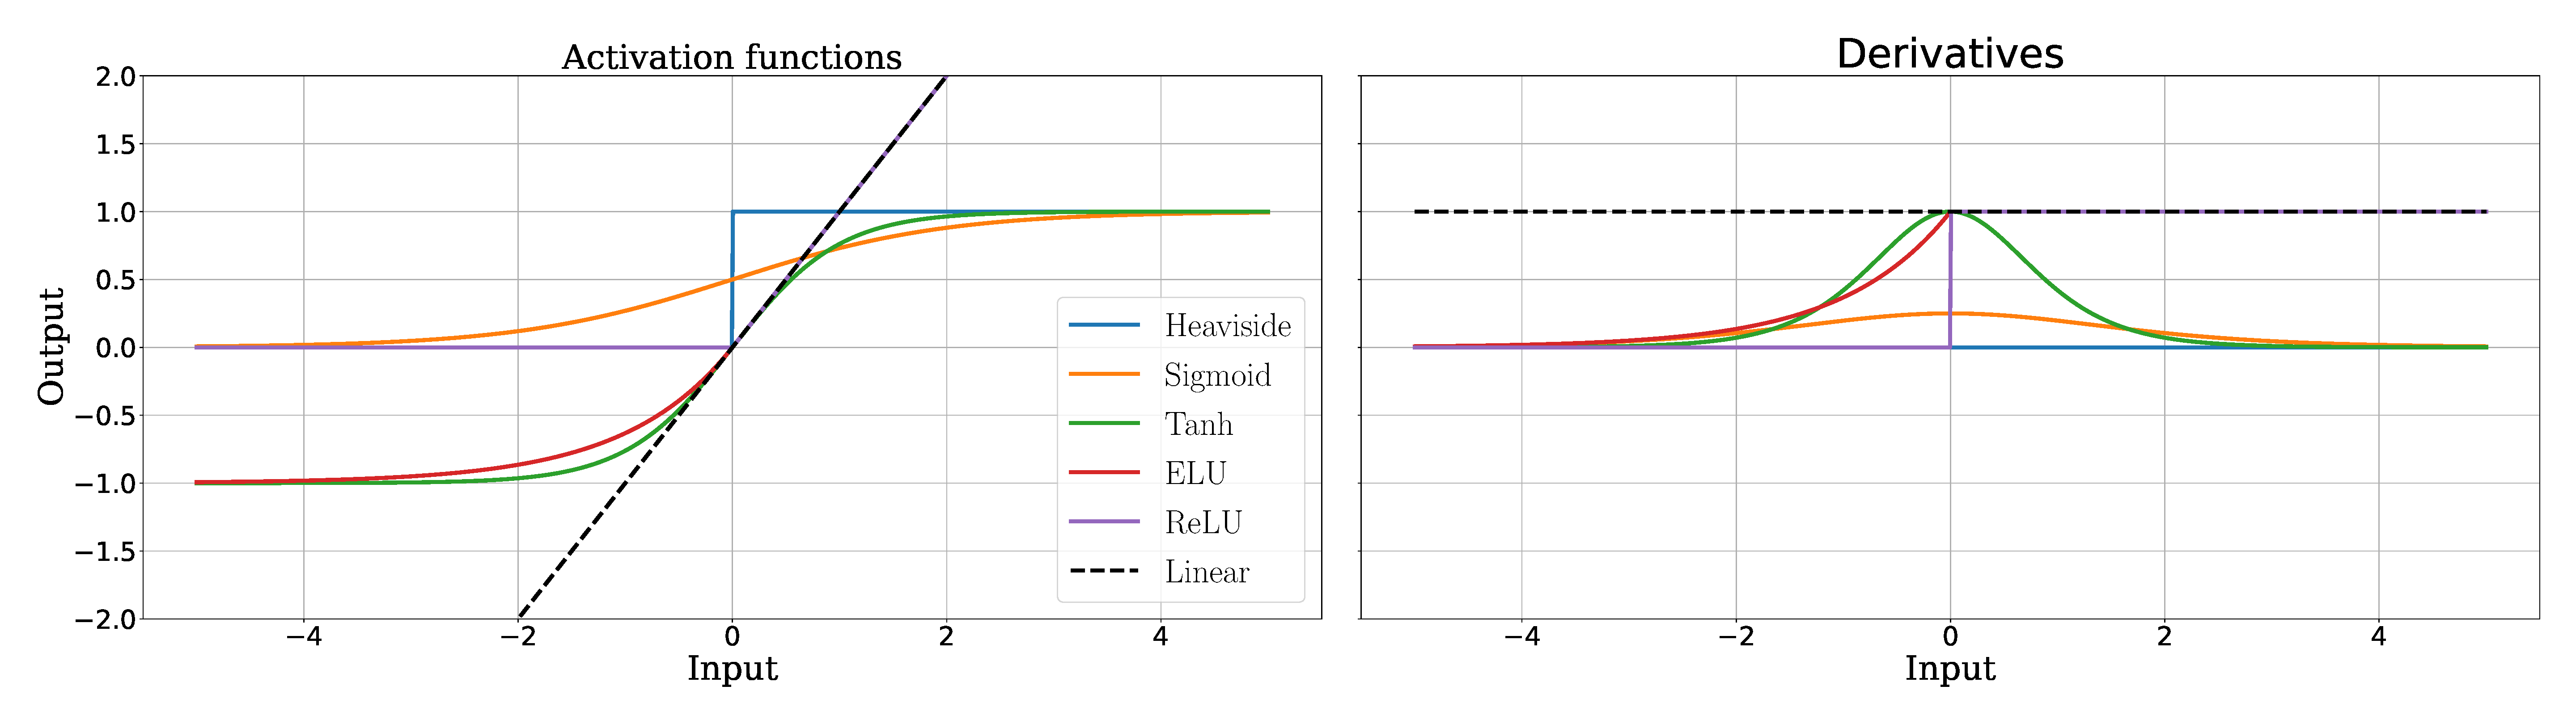
\includegraphics[width=0.98\textwidth]{chapters/foundations/sections/ml/images/activations.pdf}
	\caption[Activation functions]{A selection of different commonly used activation functions on the left and their derivatives on the right.}\label{fig:activations}
\end{figure}

With this, today's definition of a neuron is given by
\begin{equation}\label{eq:def-neuron}
n: \R^m\times \R^m\times \R \to \R;\ \lr{\vec{x}, \vec{w}, b}\mapsto a\lr{\vec{w}\cdot\vec{x} + b}.
\end{equation}
A diagram of a modern neuron is shown in \autoref{fig:neuron}. In general a \acrshort{nn} consists of arbitrary connections of these kinds of neurons, that allow for the representation of more complex functions.

\begin{figure}
	\centering
	\begin{tikzpicture}
\node[draw, circle, minimum size=0.75cm] (neuron) {};
\node (z) [below=0.1cm of neuron] {$z = \vec{w}\cdot\vec{x}+b$};
\node (x_1) [left=1.5cm of neuron] {$x_1$};
\node (x_0) [above=0.5cm of x_1] {$x_0$};
\node (x_2) [below=0.5cm of x_1] {$x_2$};
\node (a) [right=1.5cm of neuron] {$a\lr{z}$};

\draw[->, shorten >= 2pt] (x_0) -- (neuron) node[midway, above] {$w_0$};
\draw[->, shorten >= 2pt] (x_1) -- (neuron) node[midway, above] {$w_1$};
\draw[->, shorten >= 2pt] (x_2) -- (neuron) node[midway, above] {$w_2$};

\draw[->, shorten >= 2pt] (neuron) -- (a);
\end{tikzpicture}
	\caption[Single artificial neuron]{Depiction of a single neuron. It takes a three dimensional input $\vec{x}=\lr{x_0, x_1, x_2}^T$ and has four parameters; the weights $\vec{w}=\lr{w_0, w_1, w_2}^T$ and the bias $b$. Its output is the activation $a$ applied to $z=\vec{w}\cdot \vec{x}+b$.}\label{fig:neuron}
\end{figure}

However, when defining a \acrshort{nn} it is often convenient to take a more structured approach. The individual neurons can be combined into layers. Each neuron in the layer is then required to have the same inputs and the same activation function. As such a layer of neurons is a function
\begin{equation}\label{eq:def-layer}
\mathcal{L}: \R^m\times\R^{l\times m}\times\R^l\to\R^l;\ \lr{\vec{x}, W, \vec{b}}\mapsto a\lr{W\cdot \vec{x} + \vec{b}},
\end{equation}
where $W$ is the weight-matrix, consisting of the weights of each neuron stacked in the rows, and $\vec{b}$ summarizing the biases of the different neurons. The activation function $a$ is understood to operate component-wise on its argument.

To form a \acrshort{nn}, these layers can then be connected. In its most simple form, a \acrshort{nn} is a set of nested layers:
\begin{equation}\label{eq:def-fnn}
\mathcal{N}\lr{\vec{x}, \theta} = \mathcal{L}_n\lr{\mathcal{L}_{n-1}\lr{\dots \mathcal{L}_1\lr{\vec{x}, \theta_1},\dots \theta_{n-1}}, \theta_n}.
\end{equation}
The values $\theta_i = \lr{W_i, \vec{b}_i}$ are collectively called the parameters of the layer and $\theta=\lr{\theta_1, \dotsc, \theta_n}$ are the parameters of the network.

Equation \eqref{eq:def-fnn} defines a \emph{feed forward neural network}. Information flows only in one direction, from the input $x$, through the intermediate layers $\mathcal{L}_1, \mathcal{L}_2, \cdots, \mathcal{L}_{n-1}$, to the output $\mathcal{L}_n$. No feedback connections are allowed and the resulting graph is acyclic~\cite{Goodfellow:2016:DNN}. When the graph does contain cycles, the resulting network is known as a \emph{recurrent neural network} (\acrshort{rnn})~\cite{Rumelhart:1986aaa, Elman:1990aaa}. These have traditionally had many applications in different kinds of natural language processing (\acrshort{nlp})~\cite{Yin:2017aaa} and are viewed as resembling biological brains more closely. They were even considered as a central idea in the original works by McCulloch and Pitts~\cite{McCulloch:1943, Piccinini:2004}. However, feed forward \acrshort{nn}s tend to be easier to optimize than \acrshort{rnn}s and variants of feed forward \acrshort{nn}s have started to perform better than state-of-the-art \acrshort{rnn}s~\cite{Vaswani:2017aaa, Tunstall:2022aaa}. For these reasons my works have exclusively considered feed forward \acrshort{nn}s. I point the interested reader to chapter 10 of~\cite{Goodfellow:2016:DNN} and chapters 15 and 16 of~\cite{Geron:2017aaa} for more detail. When talking about \acrshort{nn}s from here on out I will exclusively refer to feed forward \acrshort{nn}s unless otherwise stated.

A \acrshort{nn} can generally be structured into three parts, as illustrated in \autoref{fig:neural_net}. The first part is the \emph{input layer} that passes its inputs unchanged. It has not been stated explicitly in the discussion above and is represented by the input vector $\vec{x}$ in equation \eqref{eq:def-fnn}. Its shape is, therefore, dictated by the example data. The final layer $\mathcal{L}_n$ is the \emph{output layer} and its shape is determined by the desired output of the network. All intermediate layers $\mathcal{L}_1$ to $\mathcal{L}_{n-1}$ in equation \eqref{eq:def-fnn} are called \emph{hidden layers}. The name stems from the fact that the use of these layers is not dictated by the data but fully determined by the learning algorithm~\cite{Goodfellow:2016:DNN}. The state is basically hidden to the outside observer, i.e. one can generally not determine the structure of the \acrshort{nn} just from considering outputs on example data. 

\begin{figure}
	\centering
	\begin{tikzpicture}[
	neuron/.style={draw, circle, minimum size=1cm},
	inp/.style={fill=blue, fill opacity=0.4, draw=blue, draw opacity=0.7},
	hid/.style={fill=Emerald, fill opacity=0.4, draw=Emerald, draw opacity=0.7},
	ops/.style={fill=red, fill opacity=0.4, draw=red, draw opacity=0.7},
	conn/.style={->, shorten >= 4pt}
]
% Input layer
\node[neuron, inp] (i0) {};
\node[neuron, inp] (i1) [below=0.5cm of i0] {};
\node[neuron, inp] (i2) [below=0.5cm of i1] {};

% Hidden layers
\node[neuron, hid] (h3) [right=1.5cm of i1] {};
\node[neuron, hid] (h2) [above=0.5cm of h3] {};
\node[neuron, hid] (h1) [above=0.5cm of h2] {};
\node[neuron, hid] (h4) [below=0.5cm of h3] {};
\node[neuron, hid] (h5) [below=0.5cm of h4] {};

\node[neuron, hid] (h12) [right=1.5cm of h1] {};
\node[neuron, hid] (h22) [right=1.5cm of h2] {};
\node[neuron, hid] (h32) [right=1.5cm of h3] {};
\node[neuron, hid] (h42) [right=1.5cm of h4] {};
\node[neuron, hid] (h52) [right=1.5cm of h5] {};

% Output layer
\node[neuron, ops] (o1) [right=1.5cm of h32] {};

%Labels
\node (x0) [left=1cm of i0] {$x_1$};
\node (x1) [left=1cm of i1] {$x_2$};
\node (x2) [left=1cm of i2] {$x_3$};

\node (out1) [right=1cm of o1] {$o_1$};

\node (helper1) [above=0.5cm of h1] {};

\node (inplay) at (i0 |- helper1) {Input layer};
\node (outlay) at (o1 |- helper1) {Output layer};
\path (inplay) -- (outlay) node[midway] (hidlay) {Hidden layers};


% Connections
% Input to hidden layer 1
\draw[conn] (i0) -- (h1);
\draw[conn] (i0) -- (h2);
\draw[conn] (i0) -- (h3);
\draw[conn] (i0) -- (h4);
\draw[conn] (i0) -- (h5);

\draw[conn] (i1) -- (h1);
\draw[conn] (i1) -- (h2);
\draw[conn] (i1) -- (h3);
\draw[conn] (i1) -- (h4);
\draw[conn] (i1) -- (h5);

\draw[conn] (i2) -- (h1);
\draw[conn] (i2) -- (h2);
\draw[conn] (i2) -- (h3);
\draw[conn] (i2) -- (h4);
\draw[conn] (i2) -- (h5);

% Hidden layer 1 to hidden layer 2
\draw[conn] (h1) -- (h12);
\draw[conn] (h1) -- (h22);
\draw[conn] (h1) -- (h32);
\draw[conn] (h1) -- (h42);
\draw[conn] (h1) -- (h52);

\draw[conn] (h2) -- (h12);
\draw[conn] (h2) -- (h22);
\draw[conn] (h2) -- (h32);
\draw[conn] (h2) -- (h42);
\draw[conn] (h2) -- (h52);

\draw[conn] (h3) -- (h12);
\draw[conn] (h3) -- (h22);
\draw[conn] (h3) -- (h32);
\draw[conn] (h3) -- (h42);
\draw[conn] (h3) -- (h52);

\draw[conn] (h4) -- (h12);
\draw[conn] (h4) -- (h22);
\draw[conn] (h4) -- (h32);
\draw[conn] (h4) -- (h42);
\draw[conn] (h4) -- (h52);

\draw[conn] (h5) -- (h12);
\draw[conn] (h5) -- (h22);
\draw[conn] (h5) -- (h32);
\draw[conn] (h5) -- (h42);
\draw[conn] (h5) -- (h52);

% Hidden 2 to output
\draw[conn] (h12) -- (o1);
\draw[conn] (h22) -- (o1);
\draw[conn] (h32) -- (o1);
\draw[conn] (h42) -- (o1);
\draw[conn] (h52) -- (o1);

% Labels to input
\draw[conn] (x0) -- (i0);
\draw[conn] (x1) -- (i1);
\draw[conn] (x2) -- (i2);

% Output to label
\draw[conn] (o1) -- (out1);
\end{tikzpicture}
	\caption[Neural network]{A  fully connected \acrshort{nn} with two hidden layers of equal size (green). It has an input layer with three neurons (blue) that accepts the input-vector $\vec{x}=\lr{x_1, x_2, x_3}^T$. Its output layer has a single neuron (red) and outputs $o_1$.}\label{fig:neural_net}
\end{figure}

The statement that the design of the hidden layers cannot be obtained from example evaluations of the network follows directly from the \emph{universal approximation theorem}. The theorem states that a feed forward \acrshort{nn} with a linear output layer and at least one hidden layer of sufficient size with a non-linear activation function\footnote{The activation function has to also be \enquote{squashing}. The common sigmoid activation for example fulfills all required conditions for the universal approximation theorem~\cite{Goodfellow:2016:DNN}.} can approximate any finite dimensional Borel measurable function to arbitrary precision~\cite{Goodfellow:2016:DNN, Hornik:1989aaa, Hornik:1990aaa}. In practical terms this means that one can always find a \acrshort{nn} $\mathcal{N}\lr{\vec{x},\theta}$ with appropriate parameters $\theta$ that can approximate a function $f\lr{\vec{x}}$. Since only a single hidden layer is required, this also means that any \acrshort{nn} $\widehat{\mathcal{N}}(\vec{x},\hat{\theta})$ can be approximated by a \acrshort{nn} $\mathcal{N}\lr{\vec{x},\theta}$ with just a single hidden layer.

One caveat of the universal approximation theorem is the size of the hidden layer. It is generally not possible to know how large it has to be to approximate any function and greater depth usually leads to better performance. Furthermore, while it is true that effectively most functions can be approximated by some \acrshort{nn}, there is no \acrshort{nn} that is the best for all tasks. This statement can be made even sharper: All \acrshort{ml} algorithms perform equally well when their performance over all possible data generating distributions is averaged~\cite{Goodfellow:2016:DNN}. %page 113
It is known as the \emph{no free lunch theorem} and was proven by Wolpert in 1996~\cite{Wolpert:1996aaa}. However, it does not state that a particular algorithm cannot outperform others for any particular task. It simply means that it is impossible to design an algorithm that is optimal for all tasks.

To conclude this subsection I want to point out that equations \eqref{eq:def-neuron}, \eqref{eq:def-layer}, and \eqref{eq:def-fnn} have only considered vector-valued inputs and functions. This is not required but simplifies notation. In \autoref{sec:cnn} layers with different inputs and outputs will be introduced.


\subsection{Training Neural Networks}\label{sec:nn-training}
The task of training a \acrshort{nn} $\mathcal{N}$ is to use example data in order to find a set of parameters $\theta$ such that $\mathcal{N}\lr{\cdot,\theta}$ suitably approximates a target function $f$. This simple statement already entails the three critical components that are required for training. First we need data sampled from the input domain of $f$. If the algorithm is supposed to be trained in a supervised manner, the corresponding outputs $f\lr{\vec{x}}$ are also required. Second, we need to quantify what it means for $\mathcal{N}$ to be a good approximation to $f$, i.e. we require a performance measure or error-function. Finally, we require a procedure to find parameters $\theta$ that minimize the error between $\mathcal{N}$ and $f$~\cite{Goodfellow:2016:DNN}. %page 149
This subsection will discuss these three aspects and will also touch on a few pitfalls that one may encounter.

The data used to train the \acrshort{nn} is called the \emph{training set}. It is a collection of discrete examples which are used to optimize the parameters $\theta$. As my work has focused solely on supervised learning tasks, for the remainder of this section I will assume that these examples contain both the input as well as the label. While a lot of what is said in this section remains true also for unsupervised learning algorithms, I refer the reader to \cite{Goodfellow:2016:DNN} for more detail.

While the training set is used to optimize the parameters of the \acrshort{nn}, we are only indirectly interested in its performance on this set. If we cared only about the predictions of the network on the training set we could simply create a lookup-table of the examples and would obtain optimal performance. Instead of remembering only the training set, we want the \acrshort{nn} to learn the underlying function $f$. To measure how good this approximation is, we have to measure the performance of the \acrshort{nn} on a second set that is sampled independently from the training set. This second set is called the \emph{test set} and the error obtained on it is known as the \emph{generalization error} or simply \emph{test error}~\cite{Goodfellow:2016:DNN}.

To be able to make statistical statements based on mathematical proofs about the ability to generalize learned features from the training set to the test set, the test set should be sampled not only independently from the training set but also be distributed identically to the training set. Collectively these conditions are called the \emph{i.i.d conditions}. In practice it is most important that the test set is as close to the real application scenario as possible. In my work the training set often consists of discrete samples, while the test set is a continuous time series. This means that both sets are fundamentally not distributed identically. However, both sets are generated with very similar assumptions and thus it is plausible that the \acrshort{nn} will be able to generalize. In fact a core result of our studies is that we are able to optimize our \acrshort{nn}s on the discrete training sets and obtain low, but marginally larger, generalization errors on the continuous test sets.

In order to measure the generalization error a performance measure is required. This performance measure is problem specific but may not always be computationally efficient to calculate or even tractable. Furthermore, for the optimization algorithms that will be discussed below it is vital that the error function is differentiable. Therefore, instead of optimizing the true performance measure one often optimizes a substitute error function instead, in the hope that the two are correlated~\cite{Goodfellow:2016:DNN}. %page 268
This error function in deep learning is known as the \emph{loss} or \emph{cost-function} and the name comes from the fact that it penalizes errors. If instead it rewards good performance, it is called the \emph{fitness function}~\cite{Geron:2017aaa}. %page 20
In deep learning the use of a loss function is more prominent. Mathematically, the loss is a function
\begin{equation}
L: \R^m\times\R^m\to\R;\ \lr{y, \hat{y}}\mapsto L\lr{y, \hat{y}},
\end{equation}
where $y$ is the label and $\hat{y}$ is the predicted output of the network. The lower the loss-values the closer the network is supposed to approximate the function. When the loss is calculated for the entire training or test set it is averaged over all examples.

For certain purposes the loss may also depend directly on other variables, most notably the parameters of the network. We ignore this case here as it is not relevant to my work, but note that including the parameters can force certain behavior of the network. For example, one can push the weights of the network to be numerically small, which can have desirable properties~\cite{Goodfellow:2016:DNN}.

While the loss can in general be freely chosen to suite the task that should be solved, it is often at least partially inspired by a maximum likelihood principle. For instance, if we assume the labels $y$ of the input data $x$ to be drawn from a normal distribution, it is sensible to train the network to estimate the mean of that distribution. Assuming further that the variance $\sigma^2$ of the underlying distribution $y=f\lr{x}$ is fixed, the network that approximates the data generating process best will be the one that maximizes the likelihood
\begin{align}\label{eq:mse-derivation}
\sum_{i=1}^M\log\left[p\lr{y_i\given x_i, \theta}\right] & = \sum_{i=1}^M\log\left[N\lr{y_i, \hat{y}_i, \sigma^2}\right]\nonumber\\
& = -M\log\left[\sigma\right] - \frac{M}{2}\log\left[2\pi\right] - \frac{1}{2\sigma^2}\sum_{i=1}^M{\left|\left|\hat{y}_i - y_i\right|\right|}^2,
\end{align}
where $\hat{y}_i = \mathcal{N}\lr{x_i, \theta}$, $N\lr{y_i, \hat{y}_i, \sigma^2}$ is the normal distribution with mean $\hat{y}_i$ and variance $\sigma^2$ evaluated at the point $y_i$, and $\lr{x_i, y_i}$ are the examples from the training set. Maximizing equation \eqref{eq:mse-derivation} by tuning only the parameters $\theta$ is equivalent to minimizing
\begin{equation}
\text{MSE} = \frac{1}{M}\sum_{i=1}^M {\left|\left|\hat{y}_i - y_i\right|\right|}^2,
\end{equation}
which is known as the \emph{mean squared error} (\acrshort{mse})~\cite{Goodfellow:2016:DNN}. %page 130
This function is commonly used as a loss in regression tasks and I have utilized it in many of my works.

Another common task in machine learning is binary classification. Defining a loss function inspired by a maximum likelihood principle in that case is not trivial, as the conditional probability, too, is binary and as such is not continuous. In this case one often uses a sigmoid activation function (see equation \eqref{eq:def-sigmoid}) on the output layer of the network and interprets the output as a probability. In this case the negative log-likelihood divided by $M$ is given by~\cite{Goodfellow:2016:DNN}%page 137
\begin{equation}
\text{Binary Cross-Entropy} = - \frac{1}{M} \sum_{i=1}^M \lr{y_i\log\left[\hat{y}_i\right]+\lr{1 - y_i}\log\left[1 - \hat{y}_i\right]},
\end{equation}
which is known as the \emph{cross-entropy loss} function or \emph{binary cross-entropy loss} function~\cite{Geron:2017aaa}. %page 149
In case the output layer has $n$ neurons and the labels are one-hot encoded, the loss can be generalized to the \emph{categorical cross-entropy}
\begin{equation}
\text{Categorical Cross-Entropy} = - \frac{1}{M} \sum_{i=1}^M \sum_{j=1}^n y_{i, j}\log\left[\hat{y}_{i, j}\right].
\end{equation}
A one-hot encoded vector has a single entry with the value of $1$, whereas the remaining entries are $0$. Alongside the \acrshort{mse}, the categorical cross-entropy was the most used loss function in my works.

The third component required to train a \acrshort{nn} is an \emph{optimizer} that adjusts the parameters $\theta$. The goal of the optimizer is to minimize the loss on the training set. \acrshort{nn}s as introduced in \autoref{sec:nn} are generally highly complex, non-linear functions that require non-convex optimization. Therefore, it is usually not possible to analytically find the optimal parameters for the network. However, if we consider a fixed example or set of examples from the training set, the loss indirectly becomes a function that depends only on the parameters of the network $\theta$. Minima of that function are extremal points and have a vanishing gradient. Furthermore, the gradient points in the direction of larger values and so one lowers the loss by taking a sufficiently small step in the opposite direction of the gradient (see \autoref{fig:gradient}). This concept is known as \emph{gradient descent} and its usage requires the existence of a derivative of the loss function~\cite{Goodfellow:2016:DNN}. % page 80
With
\begin{equation}\label{eq:total-loss}
J\lr{\theta}=\frac{1}{M}\sum_{i=1}^M L\lr{y_i, \hat{y}_i=\mathcal{N}\lr{x_i, \theta}}
\end{equation}
the parameters of the network are updated as~\cite{Goodfellow:2016:DNN}% page 
\begin{equation}\label{eq:gradient-update}
\theta\to\theta-\eta\nabla_\theta J\lr{\theta},
\end{equation}
where $\eta$ is the learning rate that controls how far the parameters are moved along the error surface of the loss function in the opposite direction of the gradient. Small values of $\eta$ lead to very accurate optimization but potentially require many steps to reach an optimal value. Large values on the other hand lead to quick improvements but risks overshooting minima~\cite{Goodfellow:2016:DNN}. %page 287
Therefore, the learning rate usually has to be adjusted by trial and error to be as large as possible while still reaching low values of the loss.

\begin{figure}
	\centering
	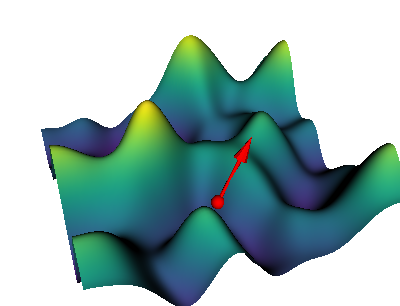
\includegraphics[width=0.6\textwidth]{chapters/foundations/sections/ml/images/gradient.png}
	\caption[Gradient]{Visualization of the gradient of a cost function for a two dimensional parameter space. The height on the vertical axis and the color represent the value of the cost function. The gradient is evaluated at the location of the red dot and is represented by the red arrow. It points in the direction of the largest positive incline. Moving a small step in the oposite direction will reduce the value of the cost function, which is the idea behind gradient descent.}\label{fig:gradient}
\end{figure}

The gradient in equation \eqref{eq:gradient-update} is calculated on the entire training set. To take multiple steps, the calculations have to be repeated on the entire training set. One such pass on the training set is called an \emph{epoch}. Since the entire training set has to be used to calculate a single step, gradient descent scales linearly with the size of that set. As it can be shown that the generalization error falls when the size of the training set increases, \acrshort{nn}s are usually trained on very large sets~\cite{Goodfellow:2016:DNN}. %page 111
This can make the use of full gradient descent computationally prohibitive.

A cheaper alternative to gradient descent is \emph{stochastic gradient descent} (\acrshort{sgd}). Instead of using the entire training set, a random subset, known as a \emph{mini-batch}, is selected. The gradient is subsequently approximated using only the examples from the mini-batch. This procedure has multiple advantages. First, it reduces the computational cost of a single update to the network parameters and forces it to be constant with regards to the size of the training set. Updating the network more often with an approximation of the gradient has proven to reduce wall-clock training time significantly~\cite{Goodfellow:2016:DNN}. %page 148/149
Second, the error between the approximate version and the full gradient scales as $1/\sqrt{n}$, where $n$ is the size of the mini-batch~\cite{Goodfellow:2016:DNN}. %page 271
It, therefore, scales slower than the cost of calculating the gradient and one can balance computational efficiency against the quality of the gradient approximation. Third, using a random subset reduces redundant calculations. In the extreme case, where all examples in the training set are the same, calculating the gradient on the entire training set is equivalent to calculating it on a single example. In a realistic case many examples from the training set may have similar effects on the gradient and applying the update to the parameters earlier leads to faster convergence ~\cite{Goodfellow:2016:DNN}. %page 271
Finally, the stochastic nature introduces randomness into the parameter update steps taken. This may be beneficial when the algorithm finds a local minimum of the loss function, which gradient descent would be unable to get out of. However, this randomness also prevents the algorithm to settle into true minima. In practice, this is a minor issue when mini-batch sizes are not too small and the advantages outweigh the drawbacks~\cite{Geron:2017aaa}. %page 124
A more sophisticated version of \acrshort{sgd} known as ``Adam'' will be discussed at the end of this subsection as it was the optimizer I primarily used in my works.

\acrshort{sgd} is not mathematically guaranteed to arrive even at a local minimum, but practical application have shown that it is capable of reaching sufficiently small values in most cases~\cite{Goodfellow:2016:DNN}. %page 150
To improve optimization further, the whole training set can be shuffled and used for another iteration of \acrshort{sgd}. Since the entire training set is reused in this case, one full pass on it is also called an epoch.

While \acrshort{sgd} describes how to change the network parameters once the gradient is known, it does not provide means to obtain it. This step was the major roadblock for deep learning which was resolved with the introduction of the \emph{backpropagation} algorithm, or simply \emph{backprop}, by Rumelhart, Hinton, and Williams in 1986~\cite{rumelhart1985:aaa}. At its core, backprop is a simple application of the chain rule of derivatives. However, it also utilizes the structured nature of the \acrshort{nn}s to save redundant calculations and thus enables an efficient computation of the gradient. Due to its importance to the field of deep learning, I will introduce the algorithm in the following paragraphs in a bit more detail.

The goal of backpropagation is to efficiently calculate $\nabla_\theta J\lr{\theta}$. For simplicity we assume $J$ to be of the form introduced in \eqref{eq:total-loss}, i.e. the loss function depends on the parameters $\theta$ only through the network. In this case we can focus on calculating the gradient of the per-example loss $L\lr{y_i, \hat{y}_i}$. For simplicity we, furthermore, assume that the output of the network $\hat{y}$ is a vector. If it is not, we apply a reshaping operation that orders the outputs to be of vector form. For readability we also drop the example index $i$ and understand that the following calculations are done for a single example. By the chain rule we then find~\cite{Goodfellow:2016:DNN}%page 199 + 205 f.
\begin{equation}\label{eq:backprop-1}
\lr{\nabla_\theta L\lr{y, \hat{y}}}_i = \frac{\partial \hat{y}^j}{\partial\theta_i} \frac{\partial L\lr{y, \hat{y}}}{\partial \hat{y}^j}=\lr{\nabla_\theta \hat{y}\cdot \nabla_{\hat{y}} L\lr{y, \hat{y}}}_i,
\end{equation}
which uses the Einstein summation convention. The rightmost part in equation \eqref{eq:backprop-1} $\nabla_{\hat{y}} L\lr{y, \hat{y}}$ is the gradient of the loss function with respect to the network output. This can be calculated analytically once and is then evaluated for each example simply by inserting the corresponding network output. The other part is the Jacobian of the network with respect to its parameters
\begin{equation}
\nabla_\theta \hat{y} = \nabla_\theta \mathcal{N}\lr{x, \theta}.
\end{equation}
We assume the network to be a simple chain of layers as defined in \eqref{eq:def-layer}. Once the backpropagation algorithm has been developed for this case, extending it to branching networks is trivial. For easier notation it is helpful to define the recursive relation $z_i\coloneqq W_i a_{i-1}\lr{z_{i-1}}+\vec{b}_i$, with the stopping condition $z_0 = x$ and $a_0$ being the identity mapping. Let $\nabla_{\theta_i}\hat{y}$ be the gradient of $\hat{y}$ only with respect to the parameters of layer $i$. With this we find
\begin{align}\label{eq:backprop_recursive}
\nabla_{\theta_i} \mathcal{N}\lr{x, \theta} = \nabla_{\theta_i}a_n\lr{z_n} & \overset{i < n}{=}\lr{\nabla_{\theta_i}z_n}\cdot\nabla_z a_n\Bigr|_{z=z_n}\nonumber\\
& \overset{\hphantom{i < n}}{=} W_n\nabla_{\theta_i}a_{n-1}\lr{z_{n-1}}\cdot\nabla_z a_n\Bigr|_{z=z_n},
\end{align}
which is a recursive relation for $\nabla_{\theta_i}a_n\lr{z_n}$ that stops on layer $i$. $n$ is the number of layers of the network. Note that while the calculations above suggest that $W_i$ have to be matrices and $z_i$ have to be vectors, the equations hold for tensors of arbitrary dimension. A few things about equation \eqref{eq:backprop_recursive} are noteworthy. First, $a_i$ are scalar functions that are applied component wise. To calculate the gradient $\nabla_z a_i$, the one-dimensional derivative $\partial_z a_i$ simply has to be evaluated at the different values of $z_i$. So the derivative for each activation function $a$ has to be computed analytically in advance only once and can then be used to rapidly calculate the gradients $\nabla_z a_i$. Second, since \eqref{eq:backprop_recursive} is a recursive equation, the gradient at layer $n-i$ depends on all gradients from layer $n-i+1$ to $n$. This is where the name backpropagation comes from, as the gradients are propagated back through the network. The recursion stops on layer $i$
\begin{equation}\label{eq:backprop-rec-stop}
\nabla_{\theta_i} a_i\lr{z_i} = \lr{\nabla_{\theta_i} W_i} a_{i-1}\lr{z_{i-1}}+\nabla_{\theta_i}\vec{b_i}.
\end{equation}

For practical implementations, the backprop algorithm is comprised of two stages. First, the input data is passed through the network and the activations $z_i$ are stored for every layer. This operation is known as the \emph{forward pass}. The second step uses the data from the forward pass to iteratively compute the gradient using equations \eqref{eq:backprop-1}, \eqref{eq:backprop_recursive}, and \eqref{eq:backprop-rec-stop}. This is referred to as the \emph{backward pass}.

In principle the calculation of the gradient could be done sequentially. In real applications this is often impractical, since \acrshort{gpu}s allow for high degrees of parallelization. Therefore, many, if not all, examples from a mini-batch are evaluated at the same time. Since the backprop algorithm requires to store the output of all intermediate layers, the memory requirements during training scale linearly with the mini-batch size. This was a limiting factor for many of our works and usually required us to use small mini-batches. Furthermore, a computational graph is usually built which describes the operations and their order that need to be taken to compute the output of the \acrshort{nn} given its input. Each node in this graph then needs to implement a backprop-method that returns the gradient of that node given any of its inputs and an inbound gradient.

As an example consider the matrix multiplication operation $C=AB$. Its backprop-method needs to return $GB^T$ when it is called for input $A$ and inbound gradient $G$ and $A^TG$ if it is called for input $B$. For a more thorough discussion of how the computational graphs are built I refer the reader to chapter 6 of~\cite{Goodfellow:2016:DNN}, where the above example was taken from.

With the definition of a training and test set, the loss function, and \acrshort{sgd} in combination with backprop we have developed the most important tools to train a \acrshort{nn}. However, during training multiple problems can arise. I will now discuss the most common ones and how to characterize them.

\subsubsection{Common problems during training}
One of the most challenging problems of deep learning is the training setup. How does one choose a network structure that is capable of efficiently solving a given problem? The structure of a \acrshort{nn} is most commonly referred to as the \emph{architecture} of the network and designing it is often more of an art than a science. Certain conditions, like translation invariance of the problem or hardware resource limitations, may inform or constrain it, but most of the time, the architecture is found empirically.

Another part of the training setup is the optimizer. It, too, can greatly influence how efficiently a \acrshort{nn} learns. Even the simple \acrshort{sgd} optimizer discussed above has a free parameter, the learning rate $\eta$. Setting it too large or too small may have detrimental results on the ability of the \acrshort{nn} to learn. More complex optimizers, such as Adam \cite{Kingma:2014aaa}, often have a larger number of tunable parameters and setting them correctly can be challenging. To find good settings for the optimizer, one usually has to resort to trial and error as well.

Both the architecture and the parameters of the optimizer have in common that they are set outside of the training loop. They can, therefore, not be updated automatically. Parameters that control the behavior of the learning algorithm are known as \emph{hyperparameters}~\cite{Goodfellow:2016:DNN}.

To optimize the hyperparameters, one often tests different settings, trains the algorithm, and compares their generalization errors. The settings that yield the best performance are then used. As we are interested in the generalization error, the training set cannot be used for this calculation. On the other hand, using the test set to optimize the hyperparameters would be dangerous, as this would introduce a bias. We would optimize the learning algorithm to perform well on the test set, reducing the ability of said set to measure how well the algorithm can generalize beyond previously observed examples. For this reason a third set is introduced: the \emph{validation set}. With this set, hyperparameters are optimized by choosing specific settings, training the resulting algorithm using the training set, and calculating the error on the validation set. The errors for different hyperparameters are subsequently compared and the model with the best performance is chosen. Finally, the generalization error is calculated on the test set only once on the chosen model to estimate how well the algorithm will perform. The error calculated on the validation set is also called the \emph{validation error}, to differentiate it from the generalization error~\cite{Goodfellow:2016:DNN}.%page 107 ff. + 117 ff.

When a \acrshort{nn} is trained for long periods of time, one can often observe that the network starts to ``remember'' the samples of the training set. To spot this, one can compare the error or loss calculated on the training set to the one calculated on the validation set after every epoch. When the network starts to remember individual samples it stops to generalize and the validation error will grow. This process is known as \emph{overfitting}~\cite{Geron:2017aaa}.%page 27 f.

To understand overfitting, we can consider polynomial regression. Let us imagine that our training set consists of $N$ samples with data $x_i$ and labels $y_i$. Let us further assume that the underlying distribution of our data is the polynomial $p(x)=\sum_{j=0}^M a_j x^j$ of degree $M < N$, i.e. $y_i=\sum_{j=0}^M a_j x_i^j$. If we use a polynomial $\hat{p}(x)=\sum_{j=0}^M \hat{a}_j x^j$ of degree $M$ to fit our training data, we will drive the \acrshort{mse} of the training set to $0$ when $\hat{a}_j = a_j\ \forall j\in\{0, 1, \cdots, M\}$. However, we can also fit all samples from the training set identically when we use a polynomial of any degree $\geq N$~\cite{Goodfellow:2016:DNN}. %page 109f.
Importantly, this fit does not necessarily have to find the coefficients
\begin{equation}
\hat{a}_j =
	\begin{cases}
		a_j,& j \leq M\\
		0,& \text{otherwise}
	\end{cases}
\end{equation}
but may find a different solution. See panels (b) and (c) of \autoref{fig:over_under_fit} for an example. In the case of overfitting the model is too complex for the task that has to be solved~\cite{Goodfellow:2016:DNN}. When the new model of degree $\geq N$ is evaluated on new points, it will most likely make incorrect predictions; it has ``memorized'' the training samples but is incapable of generalizing to new samples.

\begin{figure}
	\centering
	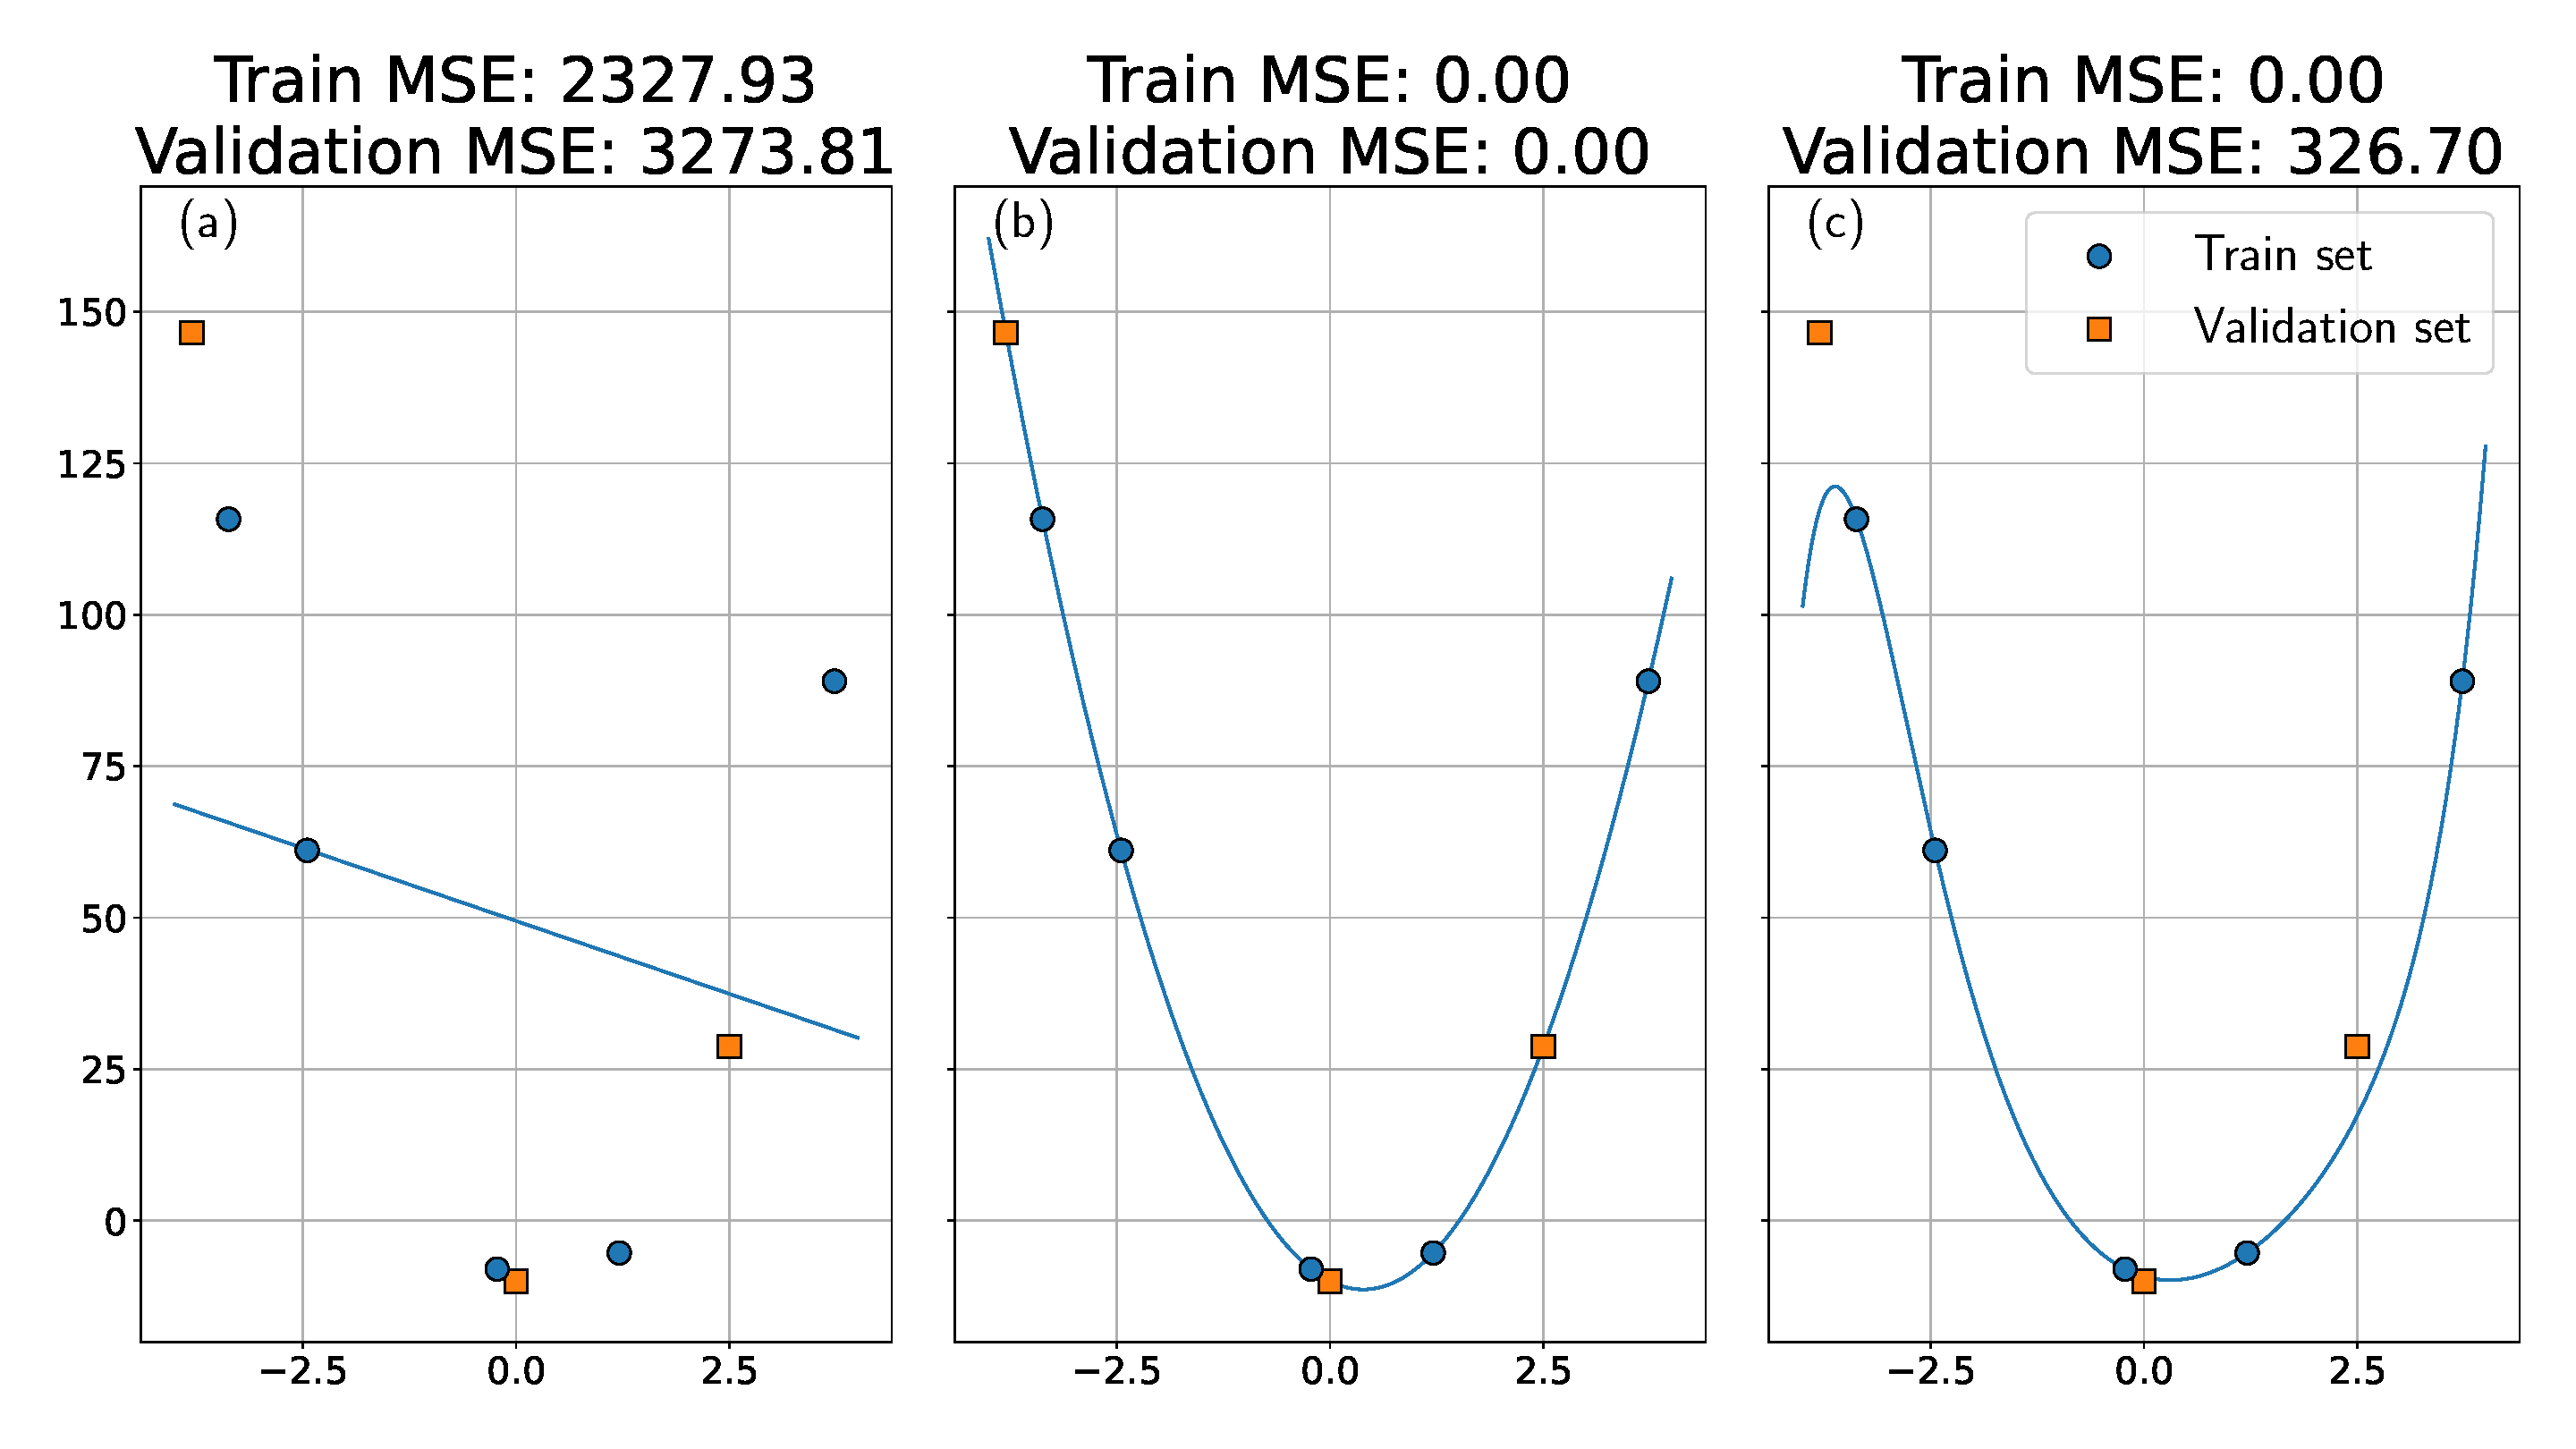
\includegraphics[width=0.98\textwidth]{chapters/foundations/sections/ml/images/overunderfit.pdf}
	\caption[Over- and underfitting]{Polynomials of different degrees fitting the same training data using a least squares fit. The training data is generated from the second degree polynomial shown in panel (b). All panels list the \acrshort{mse} of the fit against the training and validation data on top. In panel (a) a linear model is used to fit the data. It is not complex enough and underfits the data. Panel (b) is a second degree polynomial that optimally fits the data. It minimizes the \acrshort{mse} on both the training and validation set. Panel (c) fits a 9th degree polynomial to the training set. It overfits and cannot generalize well to the unseen validation data. This figure was inspired by figure 5.2 of \cite{Goodfellow:2016:DNN}.}\label{fig:over_under_fit}
\end{figure}

There are two options to reduce overfitting. One can either decrease the model complexity or increase the number of samples in the training set. As data could be generated at little additional cost for most of the studies in this work, we have usually chosen to take the latter approach~\cite{Goodfellow:2016:DNN, Geron:2017aaa}.

Instead of the model being too complex for the problem, the opposite may also happen. When the model is inherently not capable of representing the underlying data distribution, it is \emph{underfitting} the data. In the example of polynomial regression above, any polynomial of degree $<M$ would most likely be incapable of matching the training data. Panel (a) of \autoref{fig:over_under_fit} shows an example~\cite{Goodfellow:2016:DNN}.

Spotting underfitting is often a lot more challenging than spotting overfitting, because it keeps the error calculated on the training set large. However, the same effect happens, when the network has not yet converged to a good local minimum of the loss. Furthermore, one rarely knows a priory what a good value for the converged loss would be. Upper limits can often be derived, but those usually cover the network not being able to optimize at all, rather than it failing to suitably approximate the true data distribution. Once underfitting has been identified though, one can usually increase the number of trainable parameters of the \acrshort{nn} to resolve the issue. Other times finding a more suitable architecture or different data representation is required.

Another common problem of deep neural networks are vanishing or exploding gradients~\cite{Goodfellow:2016:DNN,Geron:2017aaa,He:2015aaa}. Deeper layers tend to have smaller gradients, which causes a stagnation in their optimization~\cite{Geron:2017aaa}. %page 332
To a certain degree studies have found that the main cause of vanishing gradients were the combination of the network initialization, i.e. the initial parameters of the network, and the activation functions~\cite{Glorot:2010aaa}. But even with improved network initialization and suitable activation functions, training can become difficult beyond a certain depth~\cite{He:2015aaa}.
The opposite can also happen, where gradients grow exponentially. However, this is mostly a problem in \acrshort{rnn}s and can be combated by clipping the norm of the update step~\cite{Goodfellow:2016:DNN}. %page 282


Further failure modes for the training of deep \acrshort{nn}s are discussed in chapter 8.2 of \cite{Goodfellow:2016:DNN}.


\subsubsection{The Adam Optimizer}
All of the works centered around deep learning that are discussed in this thesis make use of the Adam optimizer. For this reason, it is introduced here. Adam stands for ``adaptive moment'' estimation and it computes individual adaptive learning rates for different parameters from estimates of the first and second moments of the gradients~\cite{Kingma:2014aaa}. It can be seen as a variant to the RMSProp algorithm~\cite{Goodfellow:2016:DNN,Tieleman:2012aaa}, which extends the AdaGrad algorithm~\cite{Duchi:2011aaa}.

The core idea of AdaGrad is to scale the learning rate of individual parameters based on the scale of the gradient. In regions where the loss surface is shallow one wants to traverse it fast to reach more optimal values. In regions where the surface has a steep gradient, smaller steps should be taken to not overshoot a potential minimum. To do this, the algorithm aggregates the squared gradients. On each \acrshort{sgd} step the current gradient is then divided by the square root of the aggregated squared gradients.

RMSProp uses an exponential moving average to aggregate the squared gradients. This reduces the memory of gradients from the extreme past and helps to keep the learning rates large enough to converge quickly once a locally convex bowl has been found~\cite{Goodfellow:2016:DNN}. %page 300

Adam uses two exponential moving averages. Instead of just keeping track of the squared gradient, i.e. the second moment of the gradient, it also keeps track of the first moment of the gradient, i.e. its mean. Additionally, it removes biases from the moments. The full algorithm is given in algorithm 1 of \cite{Kingma:2014aaa}. The core calculations of the algorithm in the language used in this thesis are~\cite{Geron:2017aaa}%page 356; happens to use the same notation as me
\begin{align}
1.\ & m \leftarrow \beta_1 m - \lr{1 - \beta_1}\nabla_\theta J\lr{\theta}\nonumber\\
2.\ & s \leftarrow \beta_2 s + \lr{1 - \beta_2}\nabla_\theta J\lr{\theta}\odot\nabla_\theta J\lr{\theta}\nonumber\\
3.\ & \hat{m} \leftarrow \frac{m}{1 - \beta_1^t}\nonumber\\
4.\ & \hat{s} \leftarrow \frac{s}{1 - \beta_2^t}\nonumber\\
5.\ & \theta \leftarrow \theta + \eta\hat{m}\oslash \sqrt{\hat{s}+\epsilon},
\end{align}
where $\beta_1$, $\beta_2$, and $\epsilon$ are hyperparameters of the algorithm, $t$ counts the iterations, and $\odot$ and $\oslash$ are element wise multiplication and division operators, respectively. The default values suggested in \cite{Kingma:2014aaa} are $\beta_1 = 0.9$, $\beta_2 = 0.999$, $\epsilon = 10^-8$, and $\eta = 0.001$.

Steps $1$ and $2$ are the exponential moving averages of the first and second moment of the gradient, respectively. The values for $m$ and $s$ are both initialized as arrays filled with zeros. This initialization would introduce a bias, which is removed by the operations in steps $3$ and $4$. Finally, step $5$ applies the gradient update, which scales the learning rate by the inverse square root of the second moment of the gradients. The gradient updates are also only propagated using the running mean of step $3$.


\subsection{Convolutional Neural Networks}\label{sec:cnn}
The layers discussed in section \ref{sec:nn} connect every input to every neuron. They are known as fully connected or dense layers. A fully connected layer with $N$ inputs and $M$ outputs has a weight matrix of dimension $M\times N$. For large inputs and outputs this can quickly become very straining on both memory and compute power. Furthermore, both the input- and output-shape of the layers must be set at the beginning and cannot change.

All of these problems are being addressed by the convolutional layer which was invented in 1989~\cite{LeCun:1989aaa}. Instead of connecting all inputs to all outputs, it connects only parts of the input to each output neuron. Furthermore, the weights are shared between different connections. In mathematical terms, the layer performs a discrete convolution of a kernel with the input data; hence the name ``convolutional layer''. For 1 dimensional data $\vec{x}$, weights $\vec{w}$, and bias $b$ the layer can be written as
\begin{equation}\label{eq:1dconv_simple}
\mathcal{L}_\text{conv}\lr{x, \theta}_i = a\lr{\sum_j x_j \hat{w}_{i-j} + b},
\end{equation}
where
\begin{equation}
\hat{w}_i = 
	\begin{cases}
		w_i,& 0 \leq i < \text{dim}\lr{\vec{x}}\\
		0,& \text{otherwise}
	\end{cases}.
\end{equation}
The weights $\vec{w}$ in the above equation are often called \emph{kernel}, and when defining a \acrshort{nn} architecture with convolutional layers one often sets the \emph{kernel size}, i.e. the dimension of the kernel.

Depending on the problem, convolutional layers have several advantages over fully connected layers. First, the introduction of sparse connections. This means that not all outputs are connected to all inputs, which reduces the theoretical computational time from $\mathcal{O}\lr{M\times N}$ to $\mathcal{O}\lr{K\times N}$, where $K=\text{dim}\lr{\vec{w}}$. Second, the introduction of shared weights, which reduces memory requirements, as only $K$ rather than $M\times N$ numbers have to be stored for the weights. Third, the introduction of equivariance to translation. This is a direct consequence from sharing parameters and translating them over the input, as it allows to search for the same learned features in multiple locations of the input data. For instance, if a kernel has been optimized to detect edges in an image, it will be able to detect these edges in all parts of the image. A fully connected layer, on the other hand, would need to learn this filter at every location. While this is in principle possible, and one can reduce the convolutional layer to a special case of a fully connected layer when the input size is known\footnote{The weight vector can be zero padded to have the same dimensionality as the input vector. One then cyclicly changes the position of the weight vector in the zero padding and uses the different resulting vectors as rows for the weight matrix of a fully connected layer. See section 9.4 of \cite{Goodfellow:2016:DNN} or \cite{Schaefer:2019:MSC} for more details.}, it is not quite so simple in real applications. If we want to learn to detect a specific edge in all parts of the image, a fully connected layer needs sufficiently many examples of such edges at every location of the image. A convolutional layer might learn the filter even if the edges are only presented in one specific region of the images from the training set~\cite{Goodfellow:2016:DNN}. %page 321 ff.
Additionally, convolutional layers can process inputs of arbitrary size, as the parameters of the layer do not depend on the input.

A single kernel will learn a single filter. For example, the two dimensional filter in the top branch of \autoref{fig:edge-filter} detects vertical edges. It will, however, not be able to also detect horizontal edges. For this reason, a convolutional layer usually has multiple kernels of the same dimensions. It optimizes them in parallel to learn multiple different filters. The outputs of the convolutions with the different kernels are then stacked. The output of a single kernel convolution is known as a \emph{feature map} and the index dimension of the different feature maps is known as the \emph{channel} dimension. The name feature map originates from the observation that the activation at a certain location is particularly large, when the kernel strongly overlaps with a specific feature in the input data~\cite{Zeiler:2014aaa}. Naming different feature maps different channels, stems from RGB-images, which have three distinct channels; one for red (R), one for green (G), and one for blue (B)~\cite{Goodfellow:2016:DNN}.%page 337

\begin{figure}
	\centering
	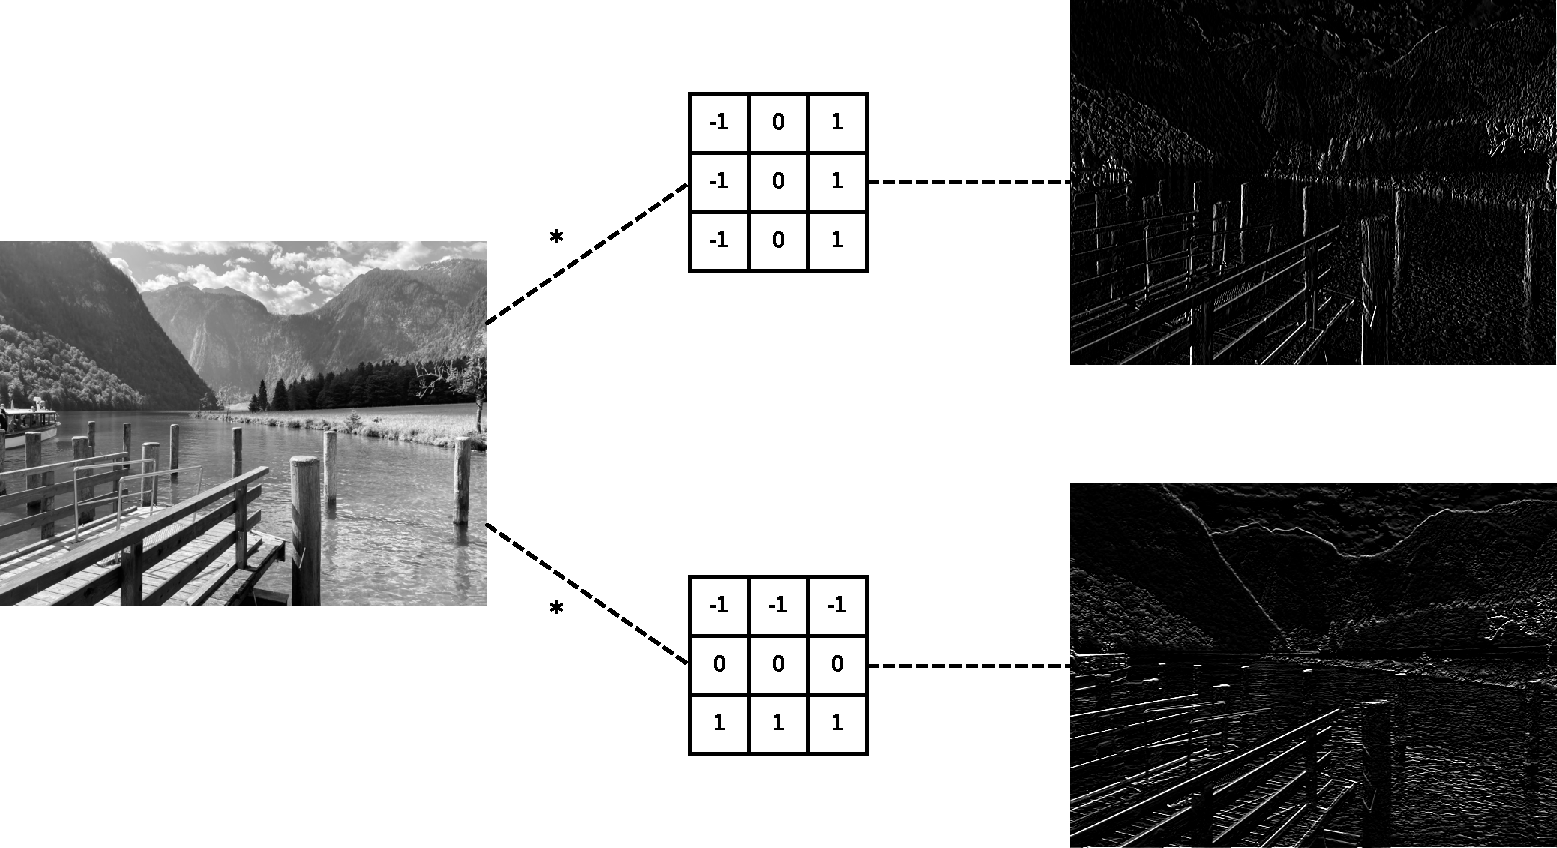
\includegraphics[width=\textwidth]{chapters/foundations/sections/ml/images/edge_filter.pdf}
	\caption[Edge detection convolution]{An image convolved with a vertical (top) and horizontal (bottom) edge-detection kernel. The original image is shown on the left. The processed images are shown on the right. The $\ast$ is the symbol for the convolution operation. Brighter pixels in the output images signify larger values, i.e. a larger overlap between the kernel and the image. On the top branch one can clearly spot the bright vertical edges of the posts, which are not visible in the lower branch. On the other hand, one can clearly spot the sharp edges at the top of the posts in the lower branch but not in the upper branch.}\label{fig:edge-filter}
\end{figure}

As was the case for \acrshort{nn}s consisting only of fully connected layers, greater depth of convolutional neural networks (\acrshort{cnn}s) allow them to detect features of greater complexity. For instance, if the first layer learns one filter for vertical edges and one for horizontal edges, a subsequent layer may use the information from both channels to infer the angle of an edge. For this to be possible, it has to combine the information. Therefore, a single kernel of a one dimensional convolution as defined in equation \eqref{eq:1dconv_simple} spans all channels. If the input to a one dimensional convolutional layer has $n$ samples and $c$ channels, a single kernel $W$ will be of dimension $k\times c$, where $k$ is the kernel size. See \autoref{fig:conv} for a visualization.

\begin{figure}
	\centering
	\begin{subfigure}[b]{.3\linewidth}
		\resizebox{\linewidth}{!}{\begin{tikzpicture}[
neuron/.style={
	regular polygon,regular polygon sides=4, minimum size=2cm, draw
}
]
% Input
\draw[solid, thick] (0, 0) rectangle (1, -1) node[pos=0.5] {$i_{1, 1}$};
\draw[solid, thick] (0, -1) rectangle (1, -2) node[pos=0.5] {$i_{2, 1}$};
\draw[solid, thick] (0, -2) rectangle (1, -3) node[pos=0.5] {$i_{3, 1}$};
\draw[solid, thick] (0, -3) rectangle (1, -4) node[pos=0.5] {$i_{4, 1}$};
\draw[solid, thick] (0, -4) rectangle (1, -5) node[pos=0.5] {$i_{5, 1}$};
\draw[solid, thick] (0, -5) rectangle (1, -6) node[pos=0.5] {$i_{6, 1}$};
\draw[solid, opacity=0] (0, -6) rectangle (1, -7);

\draw[solid, thick] (1, 0) rectangle (2, -1) node[pos=0.5] {$i_{1, 2}$};
\draw[solid, thick] (1, -1) rectangle (2, -2) node[pos=0.5] {$i_{2, 2}$};
\draw[solid, thick] (1, -2) rectangle (2, -3) node[pos=0.5] {$i_{3, 2}$};
\draw[solid, thick] (1, -3) rectangle (2, -4) node[pos=0.5] {$i_{4, 2}$};
\draw[solid, thick] (1, -4) rectangle (2, -5) node[pos=0.5] {$i_{5, 2}$};
\draw[solid, thick] (1, -5) rectangle (2, -6) node[pos=0.5] {$i_{6, 2}$};
\draw[solid, opacity=0] (1, -6) rectangle (2, -7);

% Output
\draw[solid, thick] (6, -0.5) rectangle (7, -1.5) node[pos=0.5] {$o_{1, 1}$};
\draw[solid, thick] (6, -1.5) rectangle (7, -2.5) node[pos=0.5] {$o_{2, 1}$};
\draw[solid, thick] (6, -2.5) rectangle (7, -3.5) node[pos=0.5] {$o_{3, 1}$};
\draw[solid, thick] (6, -3.5) rectangle (7, -4.5) node[pos=0.5] {$o_{4, 1}$};
\draw[solid, thick] (6, -4.5) rectangle (7, -5.5) node[pos=0.5] {$o_{5, 1}$};

\draw[solid, thick] (7, -0.5) rectangle (8, -1.5) node[pos=0.5] {$o_{1, 2}$};
\draw[solid, thick] (7, -1.5) rectangle (8, -2.5) node[pos=0.5] {$o_{2, 2}$};
\draw[solid, thick] (7, -2.5) rectangle (8, -3.5) node[pos=0.5] {$o_{3, 2}$};
\draw[solid, thick] (7, -3.5) rectangle (8, -4.5) node[pos=0.5] {$o_{4, 2}$};
\draw[solid, thick] (7, -4.5) rectangle (8, -5.5) node[pos=0.5] {$o_{5, 2}$};

\begin{scope}[on background layer]
	\draw[fill=red, fill opacity=0.3] (0, 0) rectangle (2, -2);
	\draw[fill=blue, fill opacity=0.3] (0, -3) rectangle (2, -5);
	
	\draw[fill=red, fill opacity=0.3] (6, -0.5) rectangle (7, -1.5);
	\draw[fill=blue, fill opacity=0.3] (7, -3.5) rectangle (8, -4.5);
\end{scope}

\draw[solid, draw=black] (3, 0) rectangle (4, -1) node[pos=0.5] {$w^1_{1,1}$};
\draw[solid, draw=black] (4, 0) rectangle (5, -1) node[pos=0.5] {$w^1_{1,2}$};
\draw[solid, draw=black] (3, -1) rectangle (4, -2) node[pos=0.5] {$w^1_{2,1}$};
\draw[solid, draw=black] (4, -1) rectangle (5, -2) node[pos=0.5] {$w^1_{2,2}$};

\draw[solid, draw=black] (3, -3) rectangle (4, -4) node[pos=0.5] {$w^2_{1,1}$};
\draw[solid, draw=black] (4, -3) rectangle (5, -4) node[pos=0.5] {$w^2_{1,2}$};
\draw[solid, draw=black] (3, -4) rectangle (4, -5) node[pos=0.5] {$w^2_{2,1}$};
\draw[solid, draw=black] (4, -4) rectangle (5, -5) node[pos=0.5] {$w^2_{2,2}$};

\draw[dashed, thick, draw=red] (2, 0) -- (3, 0);
\draw[dashed, thick, draw=red] (2, -2) -- (3, -2);
\draw[dashed, thick, draw=red] (5, 0) -- (6, -0.5);
\draw[dashed, thick, draw=red] (5, -2) -- (6, -1.5);

\draw[dashed, thick, draw=blue] (2, -3) -- (3, -3);
\draw[dashed, thick, draw=blue] (2, -5) -- (3, -5);
\draw[dashed, thick, draw=blue] (5, -3) -- (7, -3.5);
\draw[dashed, thick, draw=blue] (5, -5) -- (7, -4.5);
\end{tikzpicture}
}
		\caption{Convolution}\label{fig:conv}
	\end{subfigure}
	\hspace{0.03\linewidth}
	\begin{subfigure}[b]{.3\linewidth}
		\resizebox{\linewidth}{!}{\begin{tikzpicture}[
neuron/.style={
	regular polygon,regular polygon sides=4, minimum size=2cm, draw
}
]
% Input
\draw[solid, thick] (0, 0) rectangle (1, -1) node[pos=0.5] {$i_{1, 1}$};
\draw[solid, thick] (0, -1) rectangle (1, -2) node[pos=0.5] {$i_{2, 1}$};
\draw[solid, thick] (0, -2) rectangle (1, -3) node[pos=0.5] {$i_{3, 1}$};
\draw[solid, thick] (0, -3) rectangle (1, -4) node[pos=0.5] {$i_{4, 1}$};
\draw[solid, thick] (0, -4) rectangle (1, -5) node[pos=0.5] {$i_{5, 1}$};
\draw[solid, thick] (0, -5) rectangle (1, -6) node[pos=0.5] {$i_{6, 1}$};
\draw[solid, opacity=0] (0, -6) rectangle (1, -7);

\draw[solid, thick] (1, 0) rectangle (2, -1) node[pos=0.5] {$i_{1, 2}$};
\draw[solid, thick] (1, -1) rectangle (2, -2) node[pos=0.5] {$i_{2, 2}$};
\draw[solid, thick] (1, -2) rectangle (2, -3) node[pos=0.5] {$i_{3, 2}$};
\draw[solid, thick] (1, -3) rectangle (2, -4) node[pos=0.5] {$i_{4, 2}$};
\draw[solid, thick] (1, -4) rectangle (2, -5) node[pos=0.5] {$i_{5, 2}$};
\draw[solid, thick] (1, -5) rectangle (2, -6) node[pos=0.5] {$i_{6, 2}$};
\draw[solid, opacity=0] (1, -6) rectangle (2, -7);

% Output
\draw[solid, thick] (6, -1.5) rectangle (7, -2.5) node[pos=0.5] {$o_{1, 1}$};
\draw[solid, thick] (6, -2.5) rectangle (7, -3.5) node[pos=0.5] {$o_{2, 1}$};
\draw[solid, thick] (6, -3.5) rectangle (7, -4.5) node[pos=0.5] {$o_{3, 1}$};

\draw[solid, thick] (7, -1.5) rectangle (8, -2.5) node[pos=0.5] {$o_{1, 2}$};
\draw[solid, thick] (7, -2.5) rectangle (8, -3.5) node[pos=0.5] {$o_{2, 2}$};
\draw[solid, thick] (7, -3.5) rectangle (8, -4.5) node[pos=0.5] {$o_{3, 2}$};

\begin{scope}[on background layer]
	\draw[fill=red, fill opacity=0.3] (0, 0) rectangle (2, -2);
	\draw[fill=blue, fill opacity=0.3] (0, -2) rectangle (2, -4);
	\draw[fill=orange, fill opacity=0.3] (0, -4) rectangle (2, -6);
	
	\draw[fill=red, fill opacity=0.3] (6, -1.5) rectangle (7, -2.5);
	\draw[fill=blue, fill opacity=0.3] (6, -2.5) rectangle (7, -3.5);
	\draw[fill=orange, fill opacity=0.3] (6, -3.5) rectangle (7, -4.5);
\end{scope}

\draw[solid, draw=black] (3, -2) rectangle (4, -3) node[pos=0.5] {$w^1_{1,1}$};
\draw[solid, draw=black] (4, -2) rectangle (5, -3) node[pos=0.5] {$w^1_{1,2}$};
\draw[solid, draw=black] (3, -3) rectangle (4, -4) node[pos=0.5] {$w^1_{2,1}$};
\draw[solid, draw=black] (4, -3) rectangle (5, -4) node[pos=0.5] {$w^1_{2,2}$};

\draw[solid, draw=red, thick] (2, 0) -- (3, -2);
\draw[solid, draw=red, thick] (2, -2) -- (3, -4);
\draw[solid, draw=red, thick] (5, -2) -- (6, -1.5);
\draw[solid, draw=red, thick] (5, -4) -- (6, -2.5);

\draw[dashed, draw=blue, thick] (2, -2) -- (3, -2);
\draw[dashed, draw=blue, thick] (2, -4) -- (3, -4);
\draw[dashed, draw=blue, thick] (5, -2) -- (6, -2.5);
\draw[dashed, draw=blue, thick] (5, -4) -- (6, -3.5);

\draw[dotted, draw=orange, thick] (2, -4) -- (3, -2);
\draw[dotted, draw=orange, thick] (2, -6) -- (3, -4);
\draw[dotted, draw=orange, thick] (5, -2) -- (6, -3.5);
\draw[dotted, draw=orange, thick] (5, -4) -- (6, -4.5);
\end{tikzpicture}}
		\caption{Stride}\label{fig:stride}
	\end{subfigure}
	\hspace{0.03\linewidth}
	\begin{subfigure}[b]{.3\linewidth}
		\resizebox{\linewidth}{!}{\begin{tikzpicture}[
neuron/.style={
	regular polygon,regular polygon sides=4, minimum size=2cm, draw
}
]
% Input
\draw[solid, thick] (0, 0) rectangle (1, -1) node[pos=0.5] {$i_{1, 1}$};
\draw[solid, thick] (0, -1) rectangle (1, -2) node[pos=0.5] {$i_{2, 1}$};
\draw[solid, thick] (0, -2) rectangle (1, -3) node[pos=0.5] {$i_{3, 1}$};
\draw[solid, thick] (0, -3) rectangle (1, -4) node[pos=0.5] {$i_{4, 1}$};
\draw[solid, thick] (0, -4) rectangle (1, -5) node[pos=0.5] {$i_{5, 1}$};
\draw[solid, thick] (0, -5) rectangle (1, -6) node[pos=0.5] {$i_{6, 1}$};
\draw[dashed, thick] (0, -6) rectangle (1, -7) node[pos=0.5] {$0$};

\draw[solid, thick] (1, 0) rectangle (2, -1) node[pos=0.5] {$i_{1, 2}$};
\draw[solid, thick] (1, -1) rectangle (2, -2) node[pos=0.5] {$i_{2, 2}$};
\draw[solid, thick] (1, -2) rectangle (2, -3) node[pos=0.5] {$i_{3, 2}$};
\draw[solid, thick] (1, -3) rectangle (2, -4) node[pos=0.5] {$i_{4, 2}$};
\draw[solid, thick] (1, -4) rectangle (2, -5) node[pos=0.5] {$i_{5, 2}$};
\draw[solid, thick] (1, -5) rectangle (2, -6) node[pos=0.5] {$i_{6, 2}$};
\draw[dashed, thick] (1, -6) rectangle (2, -7) node[pos=0.5] {$0$};

% Output
\draw[solid, thick] (6, -0) rectangle (7, -1) node[pos=0.5] {$o_{1, 1}$};
\draw[solid, thick] (6, -1) rectangle (7, -2) node[pos=0.5] {$o_{2, 1}$};
\draw[solid, thick] (6, -2) rectangle (7, -3) node[pos=0.5] {$o_{3, 1}$};
\draw[solid, thick] (6, -3) rectangle (7, -4) node[pos=0.5] {$o_{4, 1}$};
\draw[solid, thick] (6, -4) rectangle (7, -5) node[pos=0.5] {$o_{5, 1}$};
\draw[solid, thick] (6, -5) rectangle (7, -6) node[pos=0.5] {$o_{6, 1}$};

\draw[solid, thick] (7, 0) rectangle (8, -1) node[pos=0.5] {$o_{1, 2}$};
\draw[solid, thick] (7, -1) rectangle (8, -2) node[pos=0.5] {$o_{2, 2}$};
\draw[solid, thick] (7, -2) rectangle (8, -3) node[pos=0.5] {$o_{3, 2}$};
\draw[solid, thick] (7, -3) rectangle (8, -4) node[pos=0.5] {$o_{4, 2}$};
\draw[solid, thick] (7, -4) rectangle (8, -5) node[pos=0.5] {$o_{5, 2}$};
\draw[solid, thick] (7, -5) rectangle (8, -6) node[pos=0.5] {$o_{6, 2}$};

\begin{scope}[on background layer]
	\draw[fill=red, fill opacity=0.3, draw opacity=0] (0, 0) rectangle (2, -2);
	\draw[fill=blue, fill opacity=0.3, draw opacity=0] (0, -5) rectangle (2, -7);
	
	\draw[fill=red, fill opacity=0.3] (6, 0) rectangle (7, -1);
	\draw[fill=blue, fill opacity=0.3] (6, -5) rectangle (7, -6);
\end{scope}

\draw[solid, draw=black] (3, -2) rectangle (4, -3) node[pos=0.5] {$w^1_{1,1}$};
\draw[solid, draw=black] (4, -2) rectangle (5, -3) node[pos=0.5] {$w^1_{1,2}$};
\draw[solid, draw=black] (3, -3) rectangle (4, -4) node[pos=0.5] {$w^1_{2,1}$};
\draw[solid, draw=black] (4, -3) rectangle (5, -4) node[pos=0.5] {$w^1_{2,2}$};

\draw[solid, draw=red, thick] (2, 0) -- (3, -2);
\draw[solid, draw=red, thick] (2, -2) -- (3, -4);
\draw[solid, draw=red, thick] (5, -2) -- (6, 0);
\draw[solid, draw=red, thick] (5, -4) -- (6, -1);

\draw[dashed, draw=blue, thick] (2, -5) -- (3, -2);
\draw[dashed, draw=blue, thick] (2, -7) -- (3, -4);
\draw[dashed, draw=blue, thick] (5, -2) -- (6, -5);
\draw[dashed, draw=blue, thick] (5, -4) -- (6, -6);
\end{tikzpicture}
}
		\caption{Padding}\label{fig:padding}
	\end{subfigure}
	
	\vspace{0.07\linewidth}	
	
	\begin{subfigure}[b]{.3\linewidth}
		\resizebox{\linewidth}{!}{\begin{tikzpicture}[
neuron/.style={
	regular polygon,regular polygon sides=4, minimum size=2cm, draw
}
]
% Input
\draw[solid, thick] (0, 0) rectangle (1, -1) node[pos=0.5] {$i_{1, 1}$};
\draw[solid, thick] (0, -1) rectangle (1, -2) node[pos=0.5] {$i_{2, 1}$};
\draw[solid, thick] (0, -2) rectangle (1, -3) node[pos=0.5] {$i_{3, 1}$};
\draw[solid, thick] (0, -3) rectangle (1, -4) node[pos=0.5] {$i_{4, 1}$};
\draw[solid, thick] (0, -4) rectangle (1, -5) node[pos=0.5] {$i_{5, 1}$};
\draw[solid, thick] (0, -5) rectangle (1, -6) node[pos=0.5] {$i_{6, 1}$};

\draw[solid, thick] (1, 0) rectangle (2, -1) node[pos=0.5] {$i_{1, 2}$};
\draw[solid, thick] (1, -1) rectangle (2, -2) node[pos=0.5] {$i_{2, 2}$};
\draw[solid, thick] (1, -2) rectangle (2, -3) node[pos=0.5] {$i_{3, 2}$};
\draw[solid, thick] (1, -3) rectangle (2, -4) node[pos=0.5] {$i_{4, 2}$};
\draw[solid, thick] (1, -4) rectangle (2, -5) node[pos=0.5] {$i_{5, 2}$};
\draw[solid, thick] (1, -5) rectangle (2, -6) node[pos=0.5] {$i_{6, 2}$};

% Intermediate
\draw[solid, thick] (4, 0) rectangle (5, -1) node[pos=0.5] {$h_{1, 1}$};
\draw[solid, thick] (4, -1) rectangle (5, -2) node[pos=0.5] {$h_{2, 1}$};
\draw[solid, thick] (4, -2) rectangle (5, -3) node[pos=0.5] {$h_{3, 1}$};
\draw[solid, thick] (4, -3) rectangle (5, -4) node[pos=0.5] {$h_{4, 1}$};
\draw[solid, thick] (4, -4) rectangle (5, -5) node[pos=0.5] {$h_{5, 1}$};
\draw[solid, thick] (4, -5) rectangle (5, -6) node[pos=0.5] {$h_{6, 1}$};

% Output
\draw[solid, thick] (7, 0) rectangle (8, -1) node[pos=0.5] {$o_{1, 1}$};
\draw[solid, thick] (7, -1) rectangle (8, -2) node[pos=0.5] {$o_{2, 1}$};
\draw[solid, thick] (7, -2) rectangle (8, -3) node[pos=0.5] {$o_{3, 1}$};
\draw[solid, thick] (7, -3) rectangle (8, -4) node[pos=0.5] {$o_{4, 1}$};
\draw[solid, thick] (7, -4) rectangle (8, -5) node[pos=0.5] {$o_{5, 1}$};
\draw[solid, thick] (7, -5) rectangle (8, -6) node[pos=0.5] {$o_{6, 1}$};

\begin{scope}[on background layer]
	\draw[fill=orange, fill opacity=0.3] (0, 0) rectangle (2, -5);
	
	\draw[fill=orange, fill opacity=0.3] (4, -1) rectangle (5, -4);
	
	\draw[fill=orange, fill opacity=0.3] (7, -2) rectangle (8, -3);
\end{scope}

\draw[solid, draw=black] (2, 0) -- (4, -1);
\draw[solid, draw=black] (2, -3) -- (4, -2);

\draw[dashed, draw=black] (2, -1) -- (4, -2);
\draw[dashed, draw=black] (2, -4) -- (4, -3);

\draw[solid, draw=black] (2, -2) -- (4, -3);
\draw[solid, draw=black] (2, -5) -- (4, -4);


\draw[solid, draw=black] (5, -1) -- (7, -2);
\draw[solid, draw=black] (5, -4) -- (7, -3);
\end{tikzpicture}
}
		\caption{Receptive field}\label{fig:receptive_field}
	\end{subfigure}
	\hspace{0.03\linewidth}
	\begin{subfigure}[b]{.3\linewidth}
		\resizebox{\linewidth}{!}{\begin{tikzpicture}[
neuron/.style={
	regular polygon,regular polygon sides=4, minimum size=2cm, draw
}
]
% Phantom
\draw[solid, thick, opacity=0] (0, 0) rectangle (1, -1) node[pos=0.5] {$i_{1, 1}$};
\draw[solid, thick, opacity=0] (0, -1) rectangle (1, -2) node[pos=0.5] {$i_{2, 1}$};
\draw[solid, thick, opacity=0] (0, -2) rectangle (1, -3) node[pos=0.5] {$i_{3, 1}$};
\draw[solid, thick, opacity=0] (0, -3) rectangle (1, -4) node[pos=0.5] {$i_{4, 1}$};
\draw[solid, thick, opacity=0] (0, -4) rectangle (1, -5) node[pos=0.5] {$i_{5, 1}$};
\draw[solid, thick, opacity=0] (0, -5) rectangle (1, -6) node[pos=0.5] {$i_{6, 1}$};

% Input
\draw[solid, thick] (2, 0) rectangle (3, -1) node[pos=0.5] {$i_{1, 1}$};
\draw[solid, thick] (2, -1) rectangle (3, -2) node[pos=0.5] {$i_{2, 1}$};
\draw[solid, thick] (2, -2) rectangle (3, -3) node[pos=0.5] {$i_{3, 1}$};
\draw[solid, thick] (2, -3) rectangle (3, -4) node[pos=0.5] {$i_{4, 1}$};
\draw[solid, thick] (2, -4) rectangle (3, -5) node[pos=0.5] {$i_{5, 1}$};
\draw[solid, thick] (2, -5) rectangle (3, -6) node[pos=0.5] {$i_{6, 1}$};

% Output
\draw[solid, thick] (5, -2) rectangle (6, -3) node[pos=0.5] {$o_{1, 1}$};
\draw[solid, thick] (5, -3) rectangle (6, -4) node[pos=0.5] {$o_{2, 1}$};


% Phantom
\draw[solid, thick, opacity=0] (7, 0) rectangle (8, -1) node[pos=0.5] {$o_{1, 1}$};
\draw[solid, thick, opacity=0] (7, -1) rectangle (8, -2) node[pos=0.5] {$o_{2, 1}$};
\draw[solid, thick, opacity=0] (7, -2) rectangle (8, -3) node[pos=0.5] {$o_{3, 1}$};
\draw[solid, thick, opacity=0] (7, -3) rectangle (8, -4) node[pos=0.5] {$o_{4, 1}$};
\draw[solid, thick, opacity=0] (7, -4) rectangle (8, -5) node[pos=0.5] {$o_{5, 1}$};
\draw[solid, thick, opacity=0] (7, -5) rectangle (8, -6) node[pos=0.5] {$o_{6, 1}$};

\begin{scope}[on background layer]
	\draw[fill=red, fill opacity=0.3] (2, 0) rectangle (3, -1);
	\draw[fill=red, fill opacity=0.3] (2, -2) rectangle (3, -3);
	\draw[fill=red, fill opacity=0.3] (2, -4) rectangle (3, -5);
	
	\draw[fill=blue, fill opacity=0.3] (2, -1) rectangle (3, -2);
	\draw[fill=blue, fill opacity=0.3] (2, -3) rectangle (3, -4);
	\draw[fill=blue, fill opacity=0.3] (2, -5) rectangle (3, -6);
	
	\draw[fill=red, fill opacity=0.3] (5, -2) rectangle (6, -3);
	
	\draw[fill=blue, fill opacity=0.3] (5, -3) rectangle (6, -4);
\end{scope}

\draw[solid, draw=red] (3, -0.5) -- (5, -2.5);
\draw[solid, draw=red] (3, -2.5) -- (5, -2.5);
\draw[solid, draw=red] (3, -4.5) -- (5, -2.5);

\draw[solid, draw=blue] (3, -1.5) -- (5, -3.5);
\draw[solid, draw=blue] (3, -3.5) -- (5, -3.5);
\draw[solid, draw=blue] (3, -5.5) -- (5, -3.5);
\end{tikzpicture}}
		\caption{Dilation}\label{fig:dilation}
	\end{subfigure}
\caption[Convolutional layer and its options]{\textbf{(a) Convolution:} Depiction of a 1 dimensional convolution with multiple kernels. Each kernel has the same size and spans all channels of the input. The different channels are shown as columns. Different kernels produce different channels in the output. The output in this example is calculated as $o_{a,b}=\sum_{m=1}^2\sum_{n=1}^2i_{m+a-1,n}\cdot w^b_{m,n}$. \textbf{(b) Stride:} A convolution with a stride of 2. Instead of shifting the kernel by one sample, it is shifted by multiple. The different colors relate the outputs with their inputs. \textbf{(c) Padding:} The input of the convolutional layer is padded with zeros, such that the output has the same number of samples. \textbf{(d) Receptive field:} The figure shows the neurons of two stacked convolutional layers, where padding is applied such that the input and output have the same number of samples. Both convolutional layers have a kernel size of 3. The colored squares highlight the neurons which the output $o_{3,1}$ depends on. The connecting lines for every neuron show the region of the previous layer they are directly connected to. By stacking the convolutional layers, the single output neuron $o_{3,1}$ is influenced by almost the entire input data. The part of the input a single neuron is influenced by is called its receptive field. \textbf{(e) Dilation:} Shown is a convolutional layer with a kernel that is not connected but skips a few of its input. The kernel in the figure uses only every second output and it, thus, has a dilation rate of 2. A dilation rate of $n$ means that only every $n$-th neuron from the input is considered.}\label{fig:conv_options}
\end{figure}

The definition of the convolution operation in equation \eqref{eq:1dconv_simple} shifts the kernel by a single sample for each step. However, one can just as easily implement a convolution-like operation that has a larger step size. This step size is known as the \emph{stride} and exchanges resolution for computational efficiency, as fewer computations need to be carried out~\cite{Goodfellow:2016:DNN}. The standard convolutional layer has a stride of $1$. \autoref{fig:stride} shows a strided convolution, i.e. a convolution with stride $> 1$.

When a convolutional layer with kernel size $k$ and stride $s$ is applied to input data with $n$ samples, the number of output samples $n_c$ by default is given by
\begin{equation}
	n_c = \lfloor\frac{n-k}{s}\rfloor + 1,
\end{equation}
where $\lfloor\cdot\rfloor$ is the flooring operation. For $k>1$ or $s>1$, we find $n_c<n$. So the output is smaller than the input when a convolutional layer is applied. To avoid this shrinking, one often applies \emph{padding} to the data. To pad the data one commonly uses zeros or mirrors the data at the edges. See \autoref{fig:padding} for a visualization of zero-padding.

By design, individual output neurons of a convolutional layers have only access to a small portion of their input data. This in turn limits the scale of features they may detect. To avoid this issue, one can stack multiple convolutional layers. \autoref{fig:receptive_field} shows two stacked convolutional layers, which both have a kernel size of $3$. Each output of the final convolutional layer is connected to $3$ neurons on the first layer. Each of those neurons, in turn, is connected to three input samples. As such, the output neurons have indirect access to $5$ samples from the input. This increases the amount of data they are receptive to. For this reason, the input samples each output of a convolutional layer is directly or indirectly connected to is known as its \emph{receptive field}.

Instead of connecting only subsequent samples from the input, a kernel may also skip a few samples in between. This concept is known as \emph{dilation}. It can be used to increase the scale of features a convolutional layer can detect, at the cost of resolution. The number of neurons that are skipped minus one is known as the \emph{dilation rate}. When a convolutional layer has a dilation rate of $n$, every $n$-th input sample is connected. \autoref{fig:dilation} shows how a convolutional layer with a dilation rate of $2$.

The first major application of \acrshort{cnn}s was the LeNet-5~\cite{LeCun:1998aaa}, which was used for handwriting recognition~\cite{Goodfellow:2016:DNN, Geron:2017aaa}. Since then \acrshort{cnn}s have been the major driving force in computer vision tasks such as image classification~\cite{krizhevsky:2012, Simonyan:2014aaa, Howard:2017aaa, Elharrouss:2022aaa} and object detection~\cite{Geron:2017aaa, Elharrouss:2022aaa, Girshick:2013aaa, Ren:2015aaa, Redmon:2015aaa, Liu:2016aaa}. They have also found applications in audio processing~\cite{Oord:2016wav}, \acrshort{nlp}~\cite{Yin:2017aaa}, and many scientific fields~\cite{Deiana:2021niw}. All of the works which utilized deep learning and that are part of this thesis have made use of \acrshort{cnn}s.

Convolutional layers can be easily extended to higher dimensions. When the input data has $n$ dimensions with $c$ channels, the kernel will still span all channels but be limited in size in the data dimensions. It will then be moved across the input in all dimensions to fully cover it.


\subsection{Special Layers and Concepts}
This subsection covers a few deep learning concepts that were used in different works discussed in this thesis. They go beyond fully connected and convolutional layers and are largely non-essential to gain an understanding of the works. I will, therefore, discuss them only very briefly. The interested reader may check the different sources provided below to learn more.

\subsubsection{Pooling}
One type of layer that is often used in \acrshort{cnn}s are \emph{pooling layers}. Like convolutional layers, these layers take a confined part of the input and aggregate it. The region they summarize is then shifted over the entire input. However, in contrast to dense or convolutional layers, they do usually not have any trainable parameters. They also usually operate on every channel individually and do not combine them like convolutional layers.

The two most common pooling layers are max-pooling~\cite{Ranzato:2008aaa, Gholamalinezhad:2020aaa} and average pooling~\cite{LeCun:1989aaa}. As their name suggests, they summarize a region of the input by its maximum or average value, respectively. See \autoref{fig:max_pool} for an example of pooling.

\begin{figure}
	\centering
	\begin{subfigure}[b]{.3\linewidth}
		\resizebox{\linewidth}{!}{\begin{tikzpicture}
\draw[draw=black, thick] (0, 0) rectangle (1, -1) node[pos=0.5] {$2$};
\draw[draw=black, thick] (0, -1) rectangle (1, -2) node[pos=0.5] {$4$};
\draw[draw=black, thick] (0, -2) rectangle (1, -3) node[pos=0.5] {$3$};
\draw[draw=black, thick] (0, -3) rectangle (1, -4) node[pos=0.5] {$7$};
\draw[draw=black, thick] (0, -4) rectangle (1, -5) node[pos=0.5] {$4$};

\draw[draw=black, thick] (3, -1) rectangle (4, -2) node[pos=0.5] {$4$};
\draw[draw=black, thick] (3, -2) rectangle (4, -3) node[pos=0.5] {$7$};
\draw[draw=black, thick] (3, -3) rectangle (4, -4) node[pos=0.5] {$7$};

\draw[dashed] (1, 0) -- (3, -1);
\draw[dashed] (1, -3) -- (3, -2);

\begin{scope}[on background layer]
	\draw[fill=red, fill opacity=0.3, draw opacity=0] (0, 0) rectangle (1, -3);
	
	\draw[fill=red, fill opacity=0.3, draw opacity=0] (3, -1) rectangle (4, -2);
\end{scope}
\end{tikzpicture}}
		\caption{Max pooling}\label{fig:max_pool}
	\end{subfigure}
	\hspace{0.2\linewidth}
	\begin{subfigure}[b]{.3\linewidth}
		\resizebox{\linewidth}{!}{\begin{tikzpicture}
\draw[draw=black, thick] (0, 0) rectangle (1, -1) node[pos=0.5] {$2$};
\draw[draw=black, thick] (0, -1) rectangle (1, -2) node[pos=0.5] {$4$};
\draw[draw=black, thick] (0, -2) rectangle (1, -3) node[pos=0.5] {$3$};
\draw[draw=black, thick] (0, -3) rectangle (1, -4) node[pos=0.5] {$7$};
\draw[draw=black, thick] (0, -4) rectangle (1, -5) node[pos=0.5] {$4$};

\draw[draw=black, thick] (3, -2) rectangle (4, -3) node[pos=0.5] {$4$};

\draw[dashed] (1, 0) -- (3, -2);
\draw[dashed] (1, -5) -- (3, -3);

\begin{scope}[on background layer]
	\draw[fill=red, fill opacity=0.3, draw opacity=0] (0, 0) rectangle (1, -5);
	
	\draw[fill=red, fill opacity=0.3, draw opacity=0] (3, -2) rectangle (4, -3);
\end{scope}
\end{tikzpicture}}
		\caption{Global average pooling}\label{fig:global_pool}
	\end{subfigure}
	\caption[Pooling layers]{Two kinds of pooling layers. Panel (a) shows a normal max pooling layer, that pools 3 input neurons and has a stride of 1. Panel (b) shows global average pooling, where all input neurons are pooled together.}\label{fig:pooling}
\end{figure}

Another form of pooling divides the entire input into a fixed number of bins and summarizes each bin. This form of pooling is useful, when a variable size input has to be mapped to a fixed size. This is often the case in image classifiers, where the input image is analyzed by a fully convolutional \acrshort{nn} that produces a feature map. This feature map is then passed to a fully connected classifier to extract a prediction for the classes one is interested in. See for instance the RoIPooling operation in \cite{Girshick:2015aaa} or RoIAlign in \cite{He:2017aaa}. At the extreme, all inputs are pooled together. This operation is commonly called global pooling.

The main effect of pooling layers is the introduction of an invariance to the exact location of features in the network input. By summarizing the activations in a given region, a large value anywhere within this region usually has a large value of the summary as consequence. Another effect is the downsampling of data throughout the network. This reduces the computational cost to evaluate the network, as fewer paths have to be calculated, at the expense of resolution.

\subsubsection{Dropout}
In 2014 dropout layers were introduced~\cite{Srivastava:2014aaa}. They aim to reduce overfitting during training by randomly setting the output of some neurons on hidden layers to zero, effectively erasing them from the network for one training step. See \autoref{fig:dropout} for a visualization of dropout. The rate of setting outputs to zero is known as the dropout rate and is the only hyperparameter of this layer. Erasing individual outputs has multiple beneficial effects.

\begin{figure}
	\centering
	\begin{tikzpicture}[
	neuron/.style={draw, circle, minimum size=1cm},
	inp/.style={fill=blue, fill opacity=0.4, draw=blue, draw opacity=0.7},
	hid/.style={fill=Emerald, fill opacity=0.4, draw=Emerald, draw opacity=0.7},
	ops/.style={fill=red, fill opacity=0.4, draw=red, draw opacity=0.7},
	conn/.style={->, shorten >= 4pt}
]
% Input layer
\node[neuron, inp] (i0) {};
\node[neuron, inp] (i1) [below=0.5cm of i0] {};
\node[neuron, inp] (i2) [below=0.5cm of i1] {};

% Hidden layers
\node[neuron, hid, fill opacity=0, dashed] (h3) [right=1.5cm of i1] {};
\node[neuron, hid] (h2) [above=0.5cm of h3] {};
\node[neuron, hid, fill opacity=0, dashed] (h1) [above=0.5cm of h2] {};
\node[neuron, hid] (h4) [below=0.5cm of h3] {};
\node[neuron, hid] (h5) [below=0.5cm of h4] {};

\node[neuron, hid] (h12) [right=1.5cm of h1] {};
\node[neuron, hid] (h22) [right=1.5cm of h2] {};
\node[neuron, hid] (h32) [right=1.5cm of h3] {};
\node[neuron, hid, fill opacity=0, dashed] (h42) [right=1.5cm of h4] {};
\node[neuron, hid] (h52) [right=1.5cm of h5] {};

% Output layer
\node[neuron, ops] (o1) [right=1.5cm of h32] {};

%Labels
\node (x0) [left=1cm of i0] {$x_1$};
\node (x1) [left=1cm of i1] {$x_2$};
\node (x2) [left=1cm of i2] {$x_3$};


% Connections
% Input to hidden layer 1
\draw[conn] (i0) -- (h1);
\draw[conn] (i0) -- (h2);
\draw[conn] (i0) -- (h3);
\draw[conn] (i0) -- (h4);
\draw[conn] (i0) -- (h5);

\draw[conn] (i1) -- (h1);
\draw[conn] (i1) -- (h2);
\draw[conn] (i1) -- (h3);
\draw[conn] (i1) -- (h4);
\draw[conn] (i1) -- (h5);

\draw[conn] (i2) -- (h1);
\draw[conn] (i2) -- (h2);
\draw[conn] (i2) -- (h3);
\draw[conn] (i2) -- (h4);
\draw[conn] (i2) -- (h5);

% Hidden layer 1 to hidden layer 2
\draw[conn, dashed, gray] (h1) -- (h12);
\draw[conn, dashed, gray] (h1) -- (h22);
\draw[conn, dashed, gray] (h1) -- (h32);
\draw[conn, dashed, gray] (h1) -- (h42);
\draw[conn, dashed, gray] (h1) -- (h52);

\draw[conn] (h2) -- (h12);
\draw[conn] (h2) -- (h22);
\draw[conn] (h2) -- (h32);
\draw[conn] (h2) -- (h42);
\draw[conn] (h2) -- (h52);

\draw[conn, dashed, gray] (h3) -- (h12);
\draw[conn, dashed, gray] (h3) -- (h22);
\draw[conn, dashed, gray] (h3) -- (h32);
\draw[conn, dashed, gray] (h3) -- (h42);
\draw[conn, dashed, gray] (h3) -- (h52);

\draw[conn] (h4) -- (h12);
\draw[conn] (h4) -- (h22);
\draw[conn] (h4) -- (h32);
\draw[conn] (h4) -- (h42);
\draw[conn] (h4) -- (h52);

\draw[conn] (h5) -- (h12);
\draw[conn] (h5) -- (h22);
\draw[conn] (h5) -- (h32);
\draw[conn] (h5) -- (h42);
\draw[conn] (h5) -- (h52);

% Hidden 2 to output
\draw[conn] (h12) -- (o1);
\draw[conn] (h22) -- (o1);
\draw[conn] (h32) -- (o1);
\draw[conn, dashed, gray] (h42) -- (o1);
\draw[conn] (h52) -- (o1);

% Labels to input
\draw[conn] (x0) -- (i0);
\draw[conn] (x1) -- (i1);
\draw[conn] (x2) -- (i2);

% Output to label
\draw[conn] (o1) -- (out1);
\end{tikzpicture}
	\caption[Dropout]{Visualization of \acrshort{nn} with dropout. Dashed neurons have been dropped from the graph by setting the connected dashed weights to zero.}\label{fig:dropout}
\end{figure}

First, the network is trained as a kind of ensemble of multiple networks. The different networks of the ensemble all share their architecture and weights with the network where no units are dropped, but some paths are removed. As the dropped units change for every mini-batch, each ensemble member usually is trained directly only for few iterations. Due to the shared weights, however, they are all updated simultaneously and profit from every step. During inference, no dropout is applied and as a consequence, each member of the ensemble is effectively evaluated. This can then be understood as the ensemble of all possible dropped units ``voting'' for the correct output ~\cite{Goodfellow:2016:DNN}.

Second, dropping different hidden units forces the network to become resistant to the removal of individual hidden units. It, thus, has to either learn redundancy or to classify based on different features. In a sense, dropout applies noise on the feature level. For instance, if a neuron has learned to detect a nose in a face and this neuron is dropped, the network is forced to learn to classify a face even when a nose is not present~\cite{Goodfellow:2016:DNN}.

\subsubsection{Batch Normalization}
When training a \acrshort{nn} the weights are usually updated by equation \eqref{eq:gradient-update}. The gradient $\nabla_\theta J\lr{\theta}$ is comprised of partial derivatives $\partial_{\theta_i}$, which assume that all other parameters are kept constant. However, in deep \acrshort{nn}s changing the weights on one layer will have a direct influence on the inputs to the second layer. This means that higher order effects are disregarded\footnote{Compare equation (8.34) of \cite{Goodfellow:2016:DNN}.} and the output can change a lot more than one would initially expect. In other words, the distribution of inputs to deeper layers changes as parameter updates are applied to earlier layers.

To counteract this problem, the authors of \cite{Ioffe:2015aaa} introduced a layer called \emph{Batch Normalization}. The core idea is to keep the mean and standard deviation of all or most layer outputs constant. At its core, batch normalization calculates
\begin{gather}
\mu = \frac{1}{M}\sum_{i=1}^M x_i\\
\sigma^2 = \frac{1}{M}\sum_{i=1}^M\lr{x_i - \mu}^2
\end{gather}
for every mini-batch. It then shifts the inputs by
\begin{equation}\label{eq:batch_norm_distribution_shift}
\hat{x}_i = \frac{x_i - \mu}{\sqrt{\sigma^2+\epsilon}},
\end{equation}
where $\epsilon$ is a small constant used for numerical stability. This centers the activations of the previous layer to have a mean of $0$ and a standard deviation of $1$. Crucially, the gradient takes these calculation to correct the mean and variance into account. Were this not the case, the optimization algorithm could drive the mean or the variance to infinity~\cite{Goodfellow:2016:DNN, Ioffe:2015aaa}. %page 309ff

By applying the transformation of equation \eqref{eq:batch_norm_distribution_shift} one limits the ability of the network to represent certain distributions. For instance, if the Sigmoid activation \eqref{eq:def-sigmoid} is considered, one would constrain it to the linear regime~\cite{Ioffe:2015aaa}. To allow the network to set the batch normalization layer to act as identity, the output is defined as
\begin{equation}
y_i = \gamma\hat{x}_i + \beta.
\end{equation}
The parameters $\beta$ and $\gamma$ are of the same dimension as the $x_i$ and are learned during optimization. While it may seem like a null-operation to first set the mean to $0$ and the standard deviation to $1$ and then introduce parameters $\beta$ and $\gamma$ to change the same parameters to different values, it does have a positive effect on the learning dynamics~\cite{Goodfellow:2016:DNN}.

The calculation of the mean and standard deviation described above are only done during training. For inference a running mean of these values is kept.

\subsubsection{Residual Blocks}
The submission that won the 2015 ImageNet large scale visual recognition challenge (\acrshort{ilsvrc})~\cite{Russakovsky:2015aaa} made heavy use of a concept known as \emph{residual connections}~\cite{He:2015aaa}. These residual connections allowed for their network to be effectively trained even when more than 100 stacked layers were used~\cite{He:2015aaa}. They found that the more layers could be added before training stopped being effective the larger the performance of the network. This highlights further the general notion that deeper networks usually perform better. Although introduced in 2015, their architecture is still commonly used for many state-of-the-art works today~\cite{Elharrouss:2022aaa, Lin:2017aaa, Qiao:2021aaa, Szegedy:2016aaa}.

Residual blocks contain one or multiple layers that are setup such that the blocks do not change the shape of their inputs. Their outputs are then added onto the input and passed on. See \autoref{fig:ml_residual} for a visualization. This change reformulates the learning problem. Rather than optimizing the layer block to learn a function $H\lr{x}$, one optimizes the layer block to learn the residual function $F\lr{x}=H\lr{x} - x$. While this does not change the functions that the block can represent, it changes the mapping the block learns if all parameters are driven to $0$. If the block does not use residual connections and is, hence, optimized to learn $H\lr{x}$ directly, setting all parameters to $0$ results in the zero mapping. The residual block instead would drive $F\lr{x}$ to the zero mapping, such that $H\lr{x}$ becomes the identity. Therefore, residual blocks hypothesize that an identity mapping should be the default behavior of a layer block, if it can extract no further information. This seems plausible, as one would expect that when two networks are compared, where the only difference between them is the depth, that the deeper network should not perform worse than the shallower one. In the worst case it should be able to set all of its layers at a greater depth than the shallower network to be the identity mapping~\cite{He:2015aaa}.
\begin{figure}
	\centering
	\begin{tikzpicture}
	\pgfmathsetmacro{\vertsep}{0.6}
	\pgfmathsetmacro{\bvmargin}{0.2}
    \pgfmathsetmacro{\bhmargin}{0.4}
	\node (in) {$x$};
	\node[draw, minimum width=1cm, below=\vertsep cm of in] (l1) {Layer 1};
	\node[draw, minimum width=1cm, below=\vertsep cm of l1] (l2) {Layer 2};
	\node[draw, circle, below=\vertsep cm of l2] (plus) {$+$};
	
	\draw[red, dashed] ($(l1.north west)+(-\bhmargin, \bvmargin)$) rectangle ($(l2.south east)+(\bhmargin, -\bvmargin)$);
	\node at ($(l1.north west)!0.5!(l2.south east)+(-1.7, 0)$) {$F(x)$};
    \node at ($(l1.north west)!0.5!(l2.south east)+(0.55, 0)$) {\acrshort{relu}};

    \node[below=\vertsep cm of plus] (H) {$H(x)=F(x)+x$};
    \node at ($(plus.south)!0.5!(H.north)+(0.55, 0)$) {\acrshort{relu}};

    \draw[->] ($(in)!0.5!(l1.north)$) |- ++(1.6, 0) |- (plus.east);
	
	\draw[->] (in) -- (l1.north);
	\draw[->] (l1.south) -- (l2.north);
	\draw[->] (l2.south) -- (plus.north);
    \draw[->] (plus.south) -- (H.north);
\end{tikzpicture}
	\caption[Residual block]{General structure of a residual block. The input $x$ is passed through one or multiple layers in the residual block $F(x)$ and the output is added onto its input. This figure was adapted from figure 2 in \cite{He:2015aaa}.}\label{fig:ml_residual}
\end{figure}

Another benefit of residual blocks is that they allow for an easy passing of the gradient to  layers further up in the stack. This is because the derivative of the residual block is given by
\begin{equation}
\frac{d}{dx}\lr{F\lr{x}+x} = \frac{d}{dx}F\lr{x}+1.
\end{equation}
So even if the derivative $\frac{d}{dx}F\lr{x}$ is very small, i.e. the block is close to an optimal configuration or has not started to improve yet, the additive term allows the gradient to skip past the block and propagate upwards in the network~\cite{Geron:2017aaa, He:2015aaa}. For this reason the residual blocks are also called skip connections.

\section{Machine Learning in Gravitational-Wave Astronomy}\label{sec:ml-gw-hist}
Machine learning is a computational tool that has started to gain renewed interest in the early 2010s. It is only natural for scientists to evaluate the usefulness of new tools to their own area of research. However, there are reasons beyond the academic curiousness that justify a thorough investigation of the capability of modern \acrshort{ml} algorithms to solve some of the problems in \acrshort{gw} data analysis. As previously discussed, since the first observation of a \acrshort{gw} the rate of detections has rapidly increased~\cite{Nitz:2021zwj} and is expected to grow faster as detectors are upgraded~\cite{KAGRA:2013rdx, Cahillane:2022pqm}. This necessitates the use of highly optimized data analysis algorithms to process the data in real time and produce accurate and reliable alerts. Additionally, it is desirable to produce accurate sky-maps of the expected origin of each signal to allow for prompt \acrshort{em} follow-up and to be able to extract more information from some mergers~\cite{Nitz:2020vym}. \acrshort{ml} algorithms are known for their capability to discover patterns in data and their computational efficiency has enabled many advances in other scientific fields such as computer vision~\cite{Goodfellow:2016:DNN, krizhevsky:2012}. This makes them a great contender to solve many of the above mentioned problems.

Many applications of \acrshort{ml} to \acrshort{gw} data analysis have already been studied. These include the identification and classification of glitches in the detector output, partial and full \acrshort{gw} search pipelines, and parameter estimation algorithms. Below I will give an overview of recent developments in the field and will mainly focus on algorithms relevant to \acrshort{cbc} signals. A great and more general overview of the field can be found in \cite{Cuoco:2020ogp}.

\subsection{Data Quality}
One of the first \acrshort{gw} research fields that has made use of \acrshort{ml} algorithms is the classification of data quality of the detector output~\cite{Mukherjee:2010zza, Biswas:2013wfa, Powell:2015ona, Powell:2016rkl}. As previously discussed, the detector output contains many non-Gaussian noise transients known as glitches. Finding and classifying these glitches is important to identify their source and to reduce the number of false alarms. \acrshort{ml} can be useful to identify different categories of glitches or predict them from recordings of external sensors that monitor noise sources, such as ground motion or \acrshort{em} interference~\cite{Effler:2015aaa}, which couple highly non-linearly into the detector output.

The citizen science project GravitySpy~\cite{Zevin:2016qwy} was started in 2016 and asks volunteers to classify time-frequency representations of different glitches. It leverages the Zooniverse platform and combines the use of \acrshort{ml} algorithms with human categorization to classify glitches into known and unknown categories. The resulting data sets are then used to train machine learning models~\cite{Bahaadini:2018git}. Importantly, the input data is a direct product of the detector output and does not take into account auxiliary data channels.

A different approach is taken by the iDQ pipeline, which tries to predict the presence of glitches only from auxiliary sensor data in real time~\cite{Essick:2020qpo}. It monitors $\mathcal{O}\lr{10^3}$ auxiliary channels to produce a classification into ``glitch'' or ``no-glitch'' for every time step. The underlying \acrshort{ml} algorithms are continually updated to account for non-stationarity of the noise. iDQ has been in use throughout the first three observing runs~\cite{LIGOScientific:2021djp} and contributed to the rapid release of GW170817, which coincided with a glitch~\cite{Cuoco:2020ogp}.

Other projects trying to identify glitches exist~\cite{Mukund:2016thr, Cavaglia:2018xjq, Coughlin:2019ref}, many of which rely on the time-frequency representation produced by the Omicron software package~\cite{Robinet:2020lbf}.

\subsection{Gravitational-Wave Searches}
More important for this thesis, there exists a wide variety of \acrshort{ml} based \acrshort{gw} search algorithms. It is currently a very active area of research with several groups around the world providing rapid improvements over initial algorithms. The earliest works based on random forests use data products from other search algorithms or hand crafted features to identify signals~\cite{Baker:2014eba, Kapadia:2017fhb}.

The first proof of principle using deep learning to directly detect \acrshort{bbh} signals in time series data was proposed by George et al. in 2016~\cite{George:2016hay}. They used a 3-layer \acrshort{cnn} to process \SI{1}{\second} of whitened time series data sampled at \SI{8}{\kilo\hertz} from a single detector and classified it into the two categories ``signal'' and ``noise''. Their network was trained on non-spinning \acrshort{bbh} waveforms with masses between \SI{5}{M_\odot} and \SI{75}{M_\odot}. Due to these simplifications, the parameter space consisted only of the two dimensional $m_1-m_2$-plane. For this restricted parameter space they demonstrated the ability of their algorithm to be competitive in signal recovery to matched filtering for high false-alarm probabilities (\acrshort{fap}s). As a difference to \acrshort{far}s, \acrshort{fap}s, in the context of this work, are not derived on long duration data but from individual samples that either do or do not contain a signal. The \acrshort{fap} is then the number of false positives divided by the number of true negatives. Independently, Gabbard et al. developed a similar algorithm~\cite{Gabbard:2017lja} and verified the findings of \cite{George:2016hay}. They also extended it to lower \acrshort{fap}s. Both works, however, were limited by testing the signal recovery only on discrete samples, where each sample consisted of either a well aligned waveform submerged in noise or pure noise.

The first study using deep learning to detect \acrshort{bns} signals was published by Krastev in 2019~\cite{Krastev:2019koe}. He used a network architecture similar to that of \cite{George:2016hay} to process \SI{10}{\second} sampled at \SI{4}{\kilo\hertz} to distinguish pure noise, \acrshort{bbh} signals, and \acrshort{bns} signals. He was able to reproduce the performance on \acrshort{bbh} signals from \cite{George:2016hay, Gabbard:2017lja}, but his method was significantly less sensitive to \acrshort{bns} signals. He also quoted performance figures only as a function of \acrshort{fap} derived on discrete samples rather than in terms of \acrshort{far} derived on continuous data. The study was later extended to cover real detector noise and produce point estimates for the source parameters~\cite{Krastev:2020skk}. In an independent work Schäfer et al. proposed a novel \acrshort{nn} architecture tailored toward the detection of \acrshort{bns} signals that allowed processing of \SI{32}{\second} of data~\cite{Schafer:2020kor}. To enable processing so much data, they introduced a multi-rate sampling approach, that reduced the size of the data by a factor of $9$ while preserving all relevant information. This allowed them to be substantially more sensitive than \cite{Krastev:2019koe} to low \acrshort{snr} signals. However, their approach does not generalize well to high \acrshort{snr} signals and is incapable of detecting \acrshort{bbh} signals. They also tested the algorithm on a continuous data set down to a \acrshort{far} of $0.3$ per month, thus providing a direct grounds of comparison to state-of-the-art matched filter search pipelines. It showed that there is a significant performance gap especially for low \acrshort{far}s. Furthermore, they analyzed data from two detectors in a single network. This approach is briefly summarized in chapter \ref{ch:bns} of this thesis. 

The studies discussed so far made use of a \acrshort{cnn} with a few fully connected layers to generate the classification output. This architectural choice requires the use of a sliding window approach, when the networks should be applied to data of duration longer than the input the network was trained on. Gebhard et al. introduced a fully convolutional architecture in \cite{Gebhard:2019ldz}, which allows for the network to be applied to input of arbitrary sizes. It also produces outputs with a higher time resolution than partially convolutional networks. The authors provide criticism of the evaluation procedure used in previous works, which quote performance metrics in terms of \acrshort{fap}s instead of \acrshort{far}s. They then provide extensive studies of their own  approach and test it in terms of \acrshort{far}s. They also investigate the timing accuracy of their network to the location of the merger. Their architecture was picked up and further improved by Wei et al. in \cite{Wei:2020ztw}. This improved architecture was tested on real data from \acrshort{o2} and \acrshort{o3} and is capable of detecting real \acrshort{gw} events in the data at a \acrshort{far} of $2.7$ per day. Both of these networks were also designed to process data from multiple detectors.

Another approach that has started to be explored is building \acrshort{nn}s inspired by matched filtering. Wang et al. create a convolutional layer from a reduced template bank of whitened waveforms and use it to perform a matched filter operation in the time domain~\cite{Wang:2019zaj}. Their network takes an estimate of the \acrshort{psd} into account and uses a \acrshort{cnn} to process the resulting \acrshort{snr} time series. They manage to detect all \acrshort{gw} events from \acrshort{o1} at a high \acrshort{far}. The group also contributed to the mock data challenge discussed in chapter \ref{ch:mlgwsc1}, where their approach is evaluated at low \acrshort{far}s. Yan et al. notice that matched filtering searches are formally equivalent to a particular \acrshort{nn} architecture, that can be hand crafted~\cite{Yan:2021wml}. However, they highlight that matched filtering is not optimal when the signal is not known exactly, as it is not mathematically guaranteed that it minimizes the \acrshort{far} for a given true positive rate. As a consequence, they initialize their network with a given discrete template bank and fine tune it in the hope of finding a better detection criterion. They claim that their approach can consistently outperform matched filtering. However, they test a limited mass range of \SI{40}{M_\odot} to \SI{50}{M_\odot}, where they use up to $10\,000$ templates, use only data from a single detector, and maximize over the raw \acrshort{snr} of all templates. The use of a possibly over-dense template bank, as well as the lack of coincidence and signal consistency tests artificially increase the \acrshort{far} of any detection. Nonetheless, they highlight important deficiencies of matched filtering and their work demonstrates a possible avenue for deep learning to go beyond the capability of existing methods.

The previously discussed algorithms have all made use of time series data. Most \acrshort{ml} advances, on the other hand, originate in computer vision, which processes two dimensional images. For this reason, some studies have looked at a time-frequency representation of the data to make use of such concepts. Wei et al. utilize a ResNet50~\cite{He:2015aaa} pre-trained on image classification data to create early warnings for \acrshort{bns} mergers from spectrograms of the data~\cite{Wei:2020sfz}. The network is fine tuned on injected \acrshort{gw} data and is resilient to glitches. The network is capable of detecting GW170817 \SI{10}{\second} before the merger. Aveiro et al. use the object detection network \acrshort{yolo}v5~\cite{Jocher:2022aaa} to accurately locate \acrshort{gw} mergers in these time-frequency plots. While their work is still at a proof of concept stage, this domain transform highlights an under utilized aspect of machine learning, where rapid development in other fields can improve the capability of \acrshort{gw} detection.

Some works try to utilize the computational efficiency of \acrshort{nn}s along a similar route as Wei et al.~\cite{Wei:2020sfz}. They try to produce early warnings for \acrshort{bns} signals to increase the probability of successful prompt \acrshort{em} follow-up observations. Baltus et al.~\cite{Baltus:2021nme, Baltus:2021emh} use a \acrshort{cnn} similar in nature to the early works by George et al.~\cite{George:2016hay} and Gabbard et al.~\cite{Gabbard:2017lja} to analyze time series data. In the optimal case of strong signals they expect an early warning of up to \SI{100}{\second}. Yu et al.~\cite{Yu:2021vvm} use the detector output as well as auxiliary noise channels to reduce non-linear noise couplings and increase their sensitivity to low-frequency signals. Their network is trained to produce early warnings for \acrshort{bns} and \acrshort{nsbh} signals. They claim similar early warning capabilities as Baltus et al. Chapter \ref{ch:forecasting} of this thesis summarizes a qualitative analysis of early warning capabilities of an existing state-of-the-art matched filtering based search pipeline. Such studies are important on their own but are also imperative as a point of comparison to machine learning algorithms. An advantage of the study presented in chapter \ref{ch:forecasting} over the works by Baltus et al. and Yu et al. is the capability of producing a sky-location estimate.

Besides direct searches, many studies are looking into ways to improve existing search pipelines. They mainly try to achieve this goal by adjusting the ranking statistic. Jadhav et al.~\cite{Jadhav:2020oyt} introduce MLStat, a deep learning algorithm that processes time-frequency representations of the data obtained from a continuous wavelet transform to differentiate between \acrshort{cbc} signals and glitches. The model is a pre-trained InceptionV3~\cite{Szegedy:2016aab} image classifier which is fine tuned on parts of the GravitySpy data set~\cite{Zevin:2016qwy}. They use the output of the \acrshort{cbc} class as a probability to re-weight the coincident ranking statistic and report an increase in the sensitive volume of the PyCBC search~\cite{Usman:2015kfa} by up to $30\%$. Instead of creating a new metric to adjust the ranking statistic, McIsaac et al.~\cite{McIsaac:2022odb} use deep learning to improve the existing $\chi^2$ tests. They train a \acrshort{nn} to optimize hyperparameters of a $\chi^2$ test to improve signal recovery and glitch rejection for high mass signals. They quote an improvement in sensitivity of up to $11\%$ to high total mass signals and are confident that such an automatic tuning of hyperparameters can also be used to improve other signal consistency tests. Choudhary et al.~\cite{Choudhary:2022yje} present a \acrshort{nn} that aims to distinguish \acrshort{cbc} signals from blip glitches. While they do not specify its use in altering the ranking statistic, they claim it to be superior in classification to classical $\chi^2$ tests. They introduce a sine-Gaussian projection, which produces a time-frequency representation of the data and use this as input to their network. The loosely modeled coherent wave burst (\acrshort{cwb}) search~\cite{Klimenko:2005xv, Klimenko:2015ypf} has recently introduced a \acrshort{ml} based enhancement to their pipeline~\cite{Mishra:2021tmu}. The original algorithm produces vetos based on summary statistics generated by the search to reduce the impact of non-Gaussian noise transients. These vetos are a binary decision between noise-like events and signal-like events. The \acrshort{ml} improvement uses a learning algorithm known as XGBoost~\cite{XGBoost} to create an ensemble of decision trees. A weighted average of all ensemble outputs is then processed by a Sigmoid activation to produce a continuous output. As input the decision trees use a subset of $14$ summary statistics generated by the search. By using the Sigmoid output as a modification to the original ranking statistic and by eliminating all other vetos, the authors of \cite{Mishra:2021tmu} find an improvement of up to $26\%$ in sensitivity.

Other applications of \acrshort{ml} to \acrshort{gw} searches exist. Some notable works include the application to \acrshort{cw} searches~\cite{Dreissigacker:2019edy, Dreissigacker:2020xfr, Beheshtipour:2020zhb, Beheshtipour:2020nko}, \acrshort{emri} searches~\cite{Zhang:2022xuq}, and the search for novel signals by anomaly detection~\cite{Morawski:2021kxv, Moreno:2021fvp}. The GWSkyNet project uses public data from alerts of \acrshort{gw} events intended for other astronomers for \acrshort{em} follow-up to distinguish between astrophysical events and noise artifacts~\cite{Cabero:2020eik, Abbott:2021cuf}. The aim of the project is to better inform other astronomers about which alerts are most valuable for follow-up observations.

With this plethora of different search algorithms an objective comparison among different approaches and to state-of-the-art methods is desirable. However, this task is complicated by differing data sets and the usage of different evaluation metrics. For instance, in chapter \ref{ch:bns} we find that our approach is substantially more sensitive to quite \acrshort{bns} systems than the work presented in \cite{Krastev:2019koe} but is still far away from the sensitivity of PyCBC Live, a state-of-the-art low-latency \acrshort{gw} search pipeline. For this reason, chapters \ref{ch:training_strats} and \ref{ch:cnn_coinc}, among other contributions, re-analyze the early work by Gabbard et al.~\cite{Gabbard:2017lja} and compare them to PyCBC~\cite{Usman:2015kfa}, both in the single- and multi-detector case. Chapter \ref{ch:mlgwsc1} describes an attempt of creating a reference data set and evaluation metrics to allow for the important quantification of \acrshort{ml} based search algorithm performance. It is one of the goals of this thesis to create an environment that allows for an objective evaluation of \acrshort{ml} algorithms for \acrshort{cbc} detection to enable targeted development and quick adoption of good methods into production searches.

\subsection{Parameter Estimation}
Another important aspect of \acrshort{gw} data analysis is the estimation of source parameters including error estimates. In the last three years major progress has been made in using \acrshort{ml} to rapidly produce posterior estimates. This is of special interest as traditional parameter estimation can take days or even weeks, depending on the source, to finish analyzing a single event.

As parameter estimation is not the main focus of this thesis, I will only highlight a few of the important works of the recent past. The inital work by Chua et al.~\cite{Chua:2019wwt} is capable of producing posteriors in one or two dimensions by producing histograms or parameters for a Gaussian mixture distribution. Gabbard et al.~\cite{Gabbard:2019rde} use a conditional variational autoencode network to predict the full $15$ dimensional posterior of \acrshort{bbh} directly from the whitened strain data. A variational autoencoder creates a latent representation of the input data in terms of parametrized probability distributions using an encoder. The distribution is then sampled and each sample is processed by a decoder, which in turn produces a second set of parametrized distributions. A single sample is drawn from this second set of distributions for every sample from the latent distributions. In this way a posterior is built up. Green et al.~\cite{Green:2020hst, Green:2020dnx, Dax:2021tsq} use normalizing flows to produce posteriors. The idea of a normalizing flow is to find the transformation from a simple distribution, like a Gaussian distribution, to the target distribution. In their case the target distribution is the \acrshort{gw} posterior for the parameters. They also include knowledge about symmetries of the parameters in their algorithm to simplify the task. All of these algorithms have the advantage that they do not need true posteriors as targets. Instead they learn by sampling the prior distribution during the training process. This means that training data is drawn from the prior and the networks only require the true parameter as label. Chatterjee et al.~\cite{Chatterjee:2022ggk} also use a normalizing flow for rapid sky-location estimation. It can produce accurate estimates of the source location in milliseconds. Other than previous deep learning methods it does so not only for \acrshort{bbh}, but also for \acrshort{bns} and \acrshort{nsbh} sources.

A completely different approach was taken by Williams et al.~\cite{Williams:2021qyt}. They create an algorithm named NESSAI, which is a drop in replacement for the samplers used in many state-of-the-art parameter estimation codes. Their network is also based on a normalizing flow and predicts the contours of iso-likelihood surfaces based on live-points in a nested sampling algorithm. The normalizing flow then allows them to efficiently sample the contour, resulting in an increase in the speed of nested sampling by a factor of $1.4$ over the nested sampler DYNESTY~\cite{Speagle:2020aaa}.



\chapter{Detection of Gravitational-Wave Signals from Binary Neutron Star Mergers using Machine Learning}\label{ch:bns}
\chaptermark{Binary Neutron Star Search using Machine Learning}
This chapter briefly summarizes the work done in \cite{Schafer:2020kor}, which in turn is based on my master thesis \cite{Schaefer:2019:MSC}. It highlights the improvements of \cite{Schafer:2020kor} over \cite{Schaefer:2019:MSC}. It is discussed in this thesis, as the detection of long duration \acrshort{gw} signals from \acrshort{bns} mergers is a major challenge in machine learning based search algorithms.

\section{Introduction}
Long duration \acrshort{bns} signals are computationally expensive to search for using matched filtering. This is an effect of the required high density of templates in the bank at low masses. On the other hand, detecting \acrshort{bns} signals with as low a latency as possible is important to maximize \acrshort{em} observation time of potential counterparts.

One possible approach to try to reduce computational demands of the search is to employ advanced \acrshort{ml} methods, that shift the computational cost to the training phase. To prove they are capable of rapid and accurate detection, these algorithms must be evaluated at \acrshort{far}s that are at a level comparable to online production search pipelines~\cite{Nitz:2018rgo}. In this study, we develop a deep learning search algorithm for \acrshort{bns} signals. We compare it to the PyCBC Live pipeline which has been used in the online analysis of \acrshort{o2} and \acrshort{o3}. We also compare our algorithm to another deep learning based search that targets \acrshort{bns} mergers.

The core problem of developing deep learning based \acrshort{bns} search algorithms is the duration the signal spends in the sensitive bands of the detectors. This long duration in combination with a merger at high frequencies results in a large number of samples that have to be processed. When the size of the input to a \acrshort{nn} grows, so must typically the size of the network~\cite{Goodfellow:2016:DNN}. This makes training unfeasible due to excessive hardware requirements. Our solution to this problem is to use the knowledge of the frequency evolution of \acrshort{bns} signals to re-sample different parts of the data at different rates.

\section{Methods}
To reduce the number of samples in the input to the \acrshort{nn} we sample the data at different rates. During the early inspiral the frequency is low and evolves slowly. As a consequence, a low sample rate is sufficient to resolve the signal for a long duration. Only close to the merger are high frequencies involved and a high sample rate is necessary. Informed by this signal evolution, we re-sample the first \SI{16}{\second} of the input data at a rate of \SI{128}{\hertz}. The next \SI{8}{\second} are sampled at a rate of \SI{256}{\hertz}. We continue doubling the sample rate and halving the duration of data we sample until the final second of our \SI{32}{\second} input data. The final second is split into two \SI{0.5}{\second} parts, each sampled at \SI{4096}{\hertz}. This procedure reduces the number of samples by a factor of 9, while the \acrshort{snr} that is lost due to the early truncation at low frequencies is only $\approx 2\%$. In \cite{Schaefer:2019:MSC} we had re-sampled \SI{64}{\second} by starting with a sample rate of \SI{64}{\hertz} for the first \SI{32}{\second} part. However, we found that for some signals the maximum frequency in that time period exceeded the limit of \SI{32}{\hertz} set by the sampling rate. See \autoref{fig:bns_resample} for a visualization of the re-sampling process. 
\begin{figure}
	\centering
	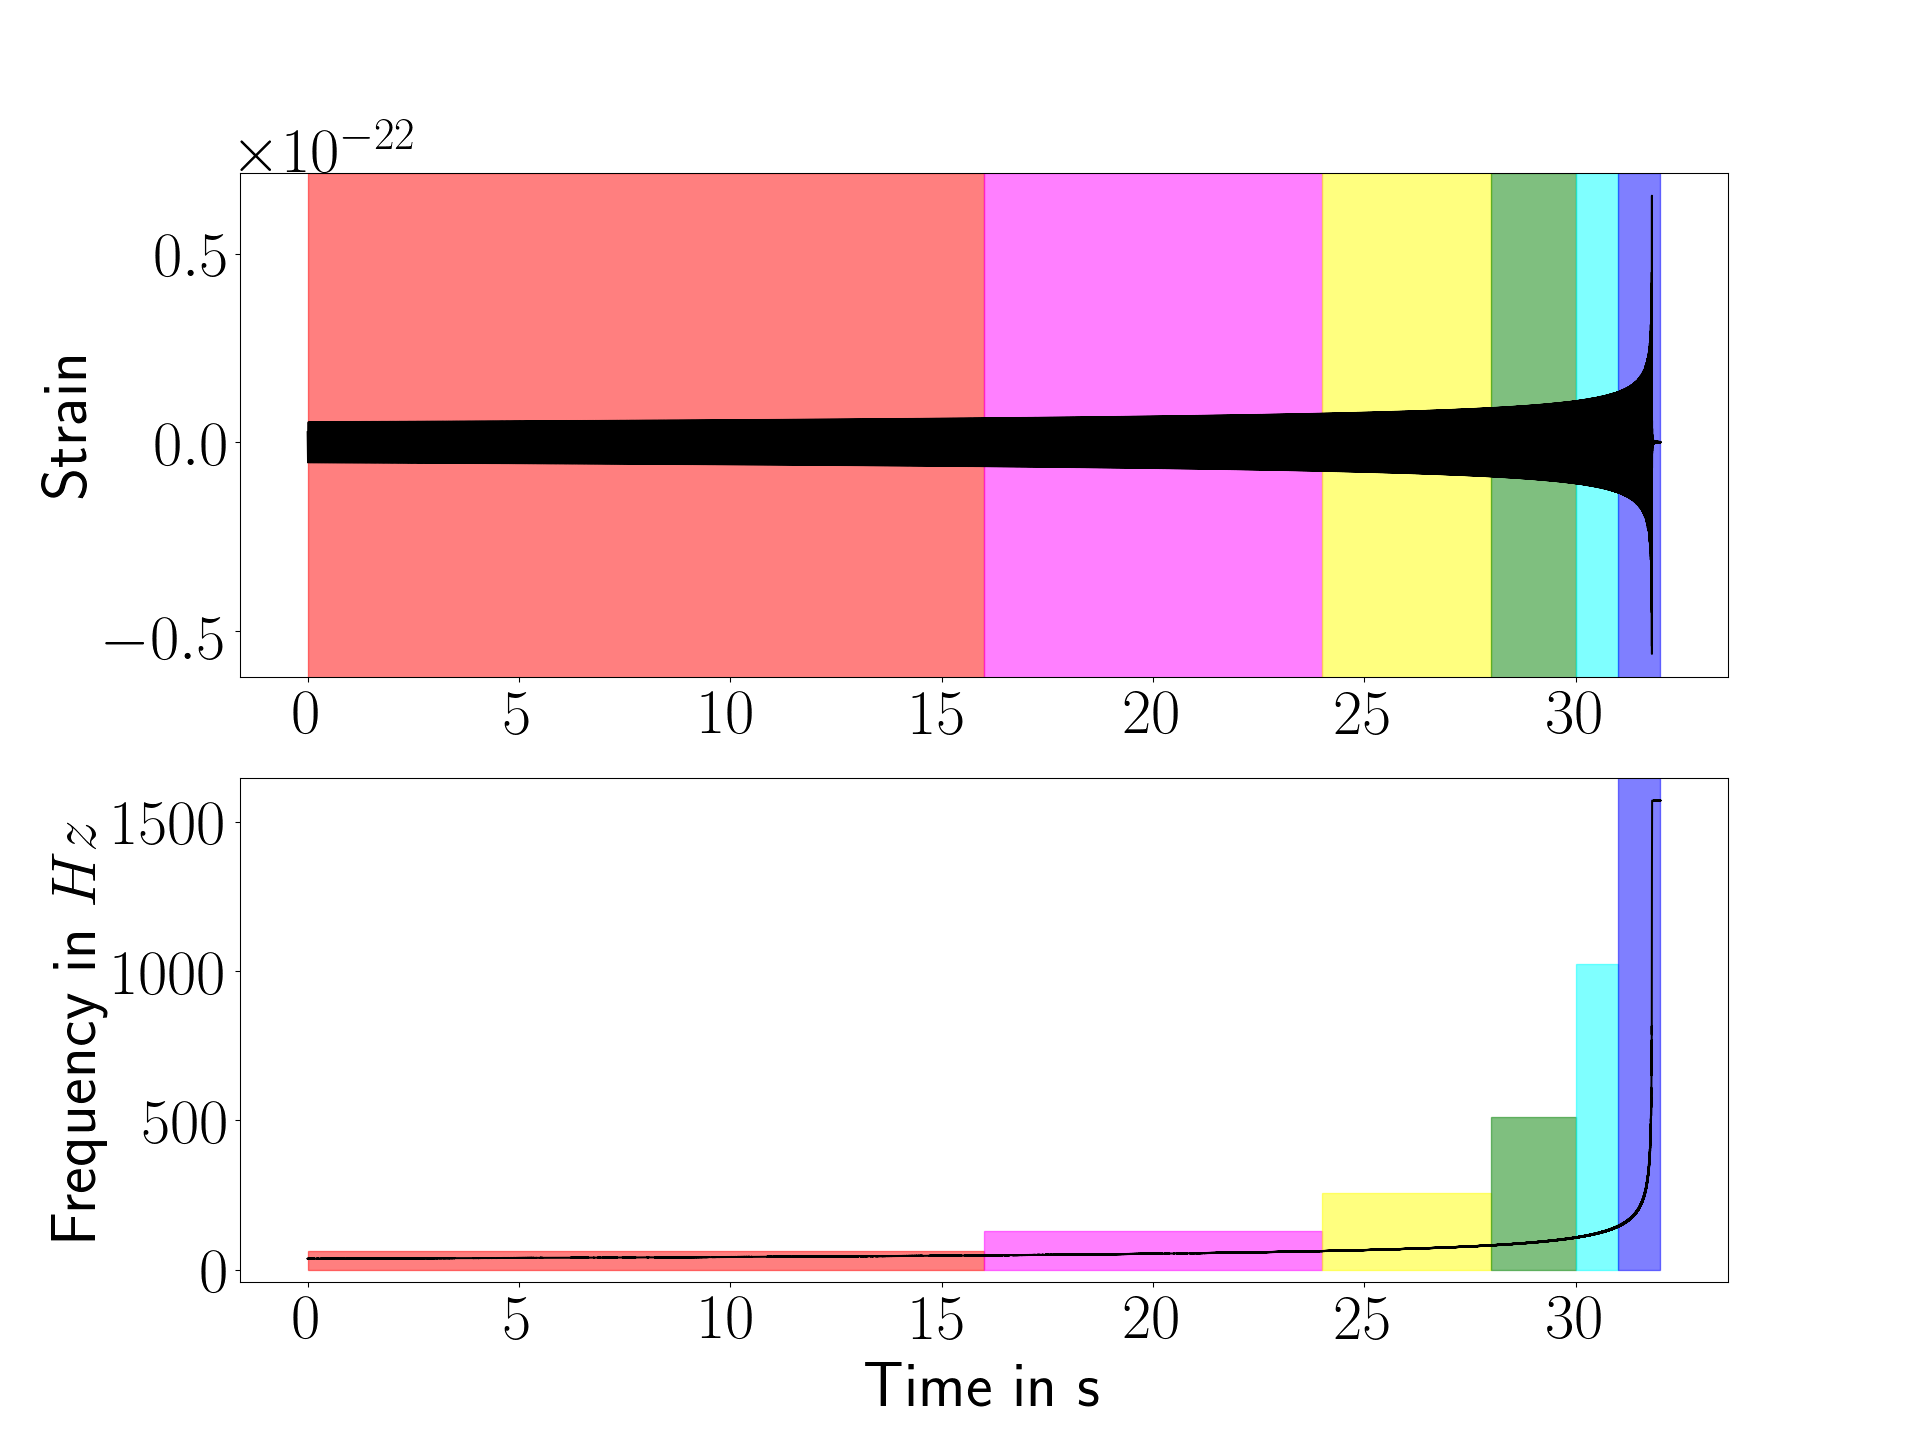
\includegraphics[width=0.8\textwidth]{chapters/bnsnet/images/resample_idea.png}
	\caption[Multi-rate sampling]{The top panel shows the strain evolution of an example \acrshort{gw} from a \acrshort{bns} merger in black. The bottom panel shows the corresponding frequency evolution in black. The colored boxes represent parts of the signal which we sample at different rates. The height of these boxes in the bottom panel represents the Nyquist-frequency of the sample rate which is used for each part. To fully resolve the signal, the black curve must stay inside the colored boxes of the bottom panel at all times. Figure and caption were taken from \cite{Schafer:2020kor}.}\label{fig:bns_resample}
\end{figure}

The architecture used in \cite{Schafer:2020kor} is highly adjusted to the multi-rate sampled data. Each of the $7$ different parts of the input data is processed by a different input to the network. After each sample rate has been processed individually, pairs of two are combined and processed further. This structure cascades down until only a single branch remains. This single branch is processed by a few more layers to produce two outputs: An estimate of the optimal \acrshort{snr} contained in the input and a p-score that is a value between $0$ and $1$ signifying the confidence of the network that a signal is present in the input. A high-level overview of the architecture is given in \autoref{fig:bns_architecture}. For more details see \cite{Schafer:2020kor, Schaefer:2019:MSC}. The architecture is the same as the one presented in \cite{Schaefer:2019:MSC}, adjusted to the reduced number of multi-rate sampled parts.
\begin{sidewaysfigure*}
	\centering
	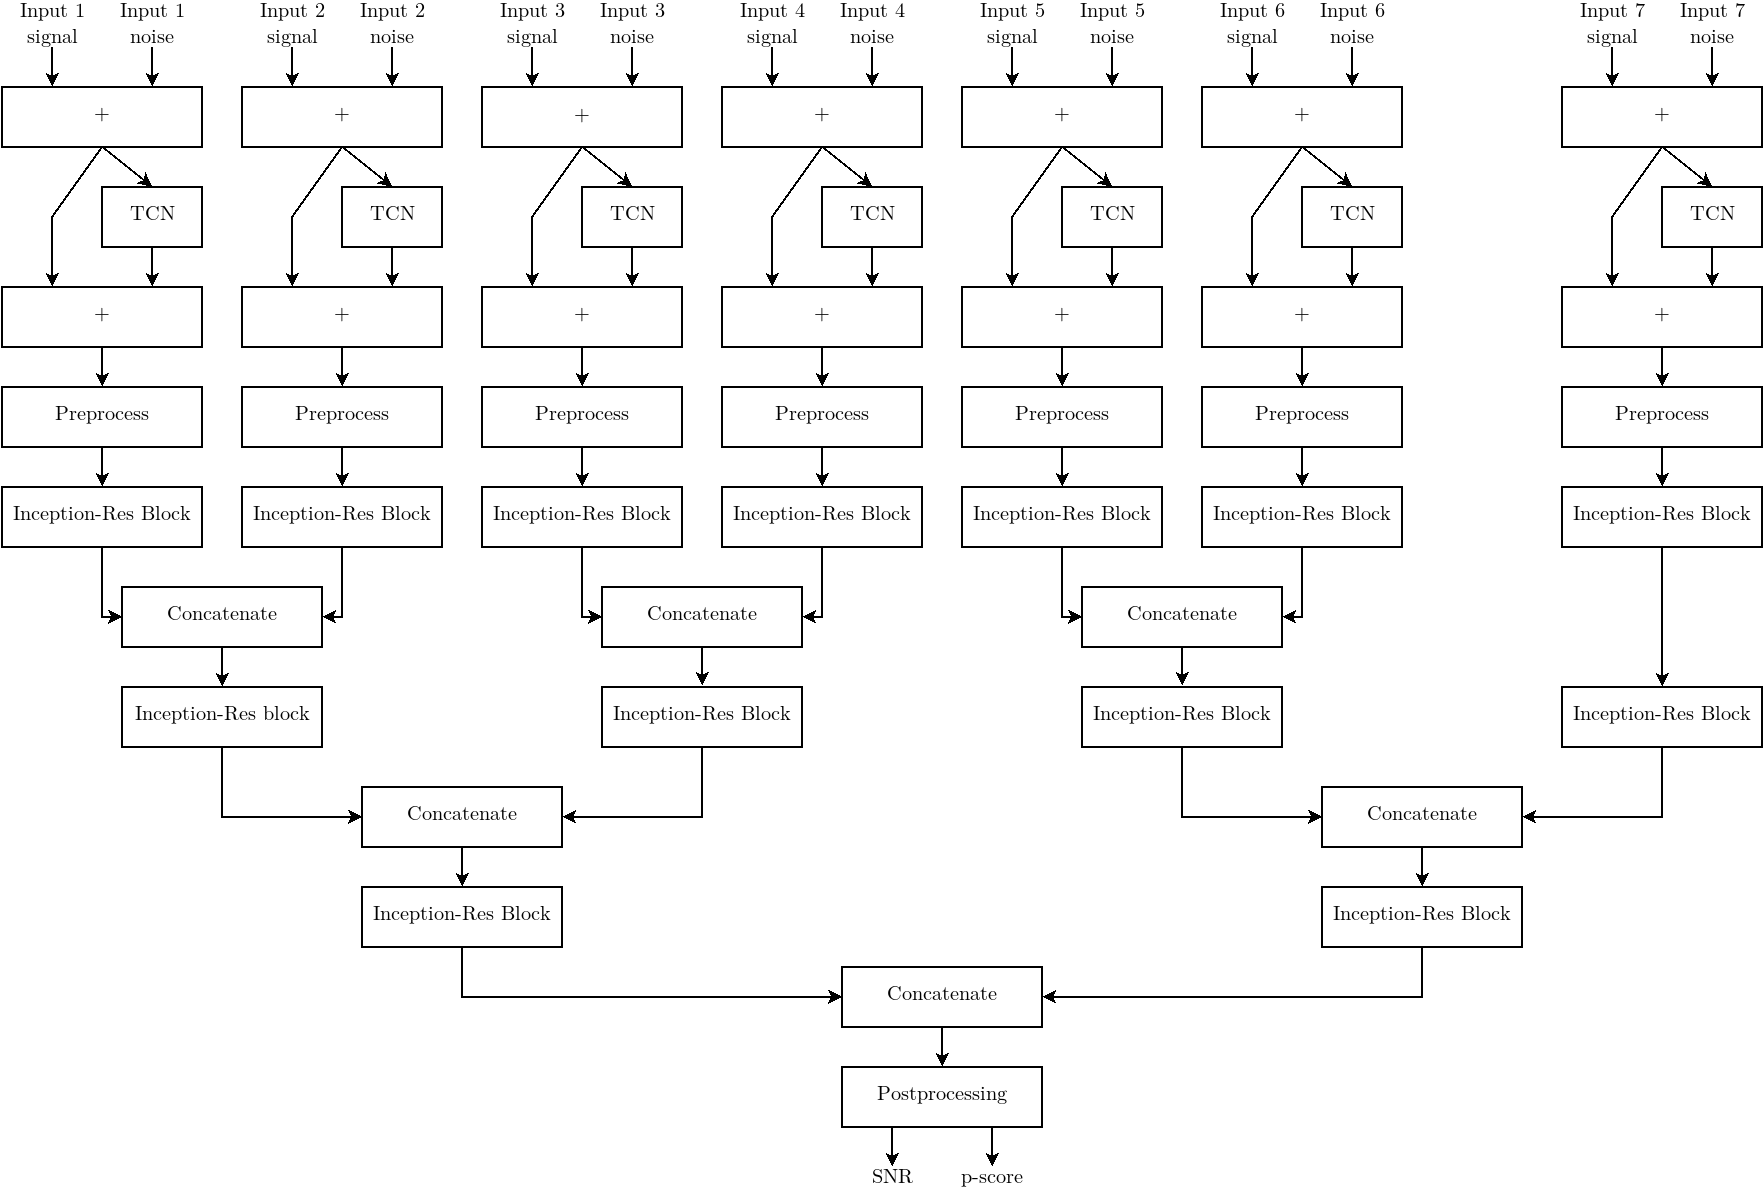
\includegraphics[width=0.9\textwidth]{chapters/bnsnet/images/architecture.png}
	\caption[Architecture]{A high level overview of the architecture presented in \cite{Schafer:2020kor}. Details on every block can be found in \cite{Schaefer:2019:MSC}. The network takes signal and noise inputs $1$ to $7$, where each number corresponds to a different part of the re-sampled raw data. It outputs an estimate of the \acrshort{snr} contained in the input and a p-score, which rates how likely the data is to contain a \acrshort{bns} signal. Figure and caption were taken from \cite{Schafer:2020kor}.}\label{fig:bns_architecture}
\end{sidewaysfigure*}

Training and validation data were created by the same process. Noise is simulated from the advanced \acrshort{ligo} design sensitivity curve in its zero detuned high-power configuration~\cite{lalsuite}. Signals are generated using the TaylorF2 waveform approximant~\cite{Droz:1999qx, Blanchet:2006aaa, Faye:2012we}, with all parameters except for the distance $r$ drawn from \autoref{tab:bns_parameter_distribution}. The distance is set indirectly by fixing the optimal \acrshort{snr} to a value uniformly drawn between $8$ and $15$. For each sample in the training set, we generate \SI{96}{\second} of data, whiten it by the \acrshort{psd} model, and crop the resulting data to \SI{32}{\second}. The exact position of the merger time in the final data is varied by \SI[parse-numbers=false]{\pm 0.25}{\second}. We create noise for the \acrshort{ligo}-Hanford and \acrshort{ligo}-Livingston detectors and inject the projected waveforms into both. The test set consists of $\approx 101$ days of continuous data split into multiple files. Injections are generated using the same waveform model and the distributions of \autoref{tab:bns_parameter_distribution}. They are spaced by \SIrange{180}{220}{\second}. Our work in \cite{Schafer:2020kor} corrects an error from \cite{Schaefer:2019:MSC} where the \acrshort{psd} was sampled too coarsely. This reduced the \acrshort{snr} of the signals below the expected value.
\begin{table}
\centering
\begin{tabular}{ll}
	\hline\hline
    parameter & uniform distribution\\
    \hline\\
    component masses & \SI[parse-numbers=false]{m_1, m_2\in\left(1.2,1.6\right)}{M_\odot}\\
    spins & 0\\
    coalescence phase & $\Phi_0\in\left(0, 2\pi\right)$\\
    polarization & $\Psi\in\left(0, 2\pi\right)$\\
    inclination & $\cos{\iota}\in\left(-1, 1\right)$\\
    declination & $\sin{\theta}\in\left(-1, 1\right)$\\
    right ascension & $\varphi\in\left(-\pi, \pi\right)$\\
    distance & \SI[parse-numbers=false]{r^2\in\left(0^2, 400^2\right)}{{\mega\parsec}^2}\\
    \hline\hline
\end{tabular}
\caption[Parameter distributions]{The astrophysically motivated distribution of parameters used to generate injections. These are used to estimate the \acrshort{far} and sensitivity of the search algorithm specified in \cite{Schafer:2020kor}. Table and caption were taken from \cite{Schafer:2020kor}.}\label{tab:bns_parameter_distribution}
\end{table}

To apply the network to data of duration longer than the input, i.e. \SI{32}{\second}, a sliding window is used. Each window is whitened and re-sampled as described above. The window uses a step size of \SI{0.25}{\second}, matching the variation of the merger time in the training data. The outputs of the network are time series of \acrshort{snr} estimates and p-scores. We apply thresholds of \acrshort{snr} $4$ and p-score $0.1$ and cluster points exceeding the threshold if they are within \SI{1}{\second} of each other. Afterward, we compare the time of the maximum value of each cluster with the injections to determine true and false positive detections. We accept something as true positive, if it is within \SI{3}{\second} of an injection.

\section{Results}
The sensitivity of our proposed algorithm is summarized in \autoref{fig:bns_sensitivity}. Our testing procedure allows us to calculate sensitivities down to a \acrshort{far} of $0.3$ per month. We find that the \acrshort{snr} output collapses to zero sensitivity below a \acrshort{far} of $0.6$ per month, while the p-score collapses already at a \acrshort{far} of $12$ per month. This is an improvement over \cite{Schaefer:2019:MSC}, which was incapable of resolving \acrshort{far}s below $30$ per month. The algorithm shows non negligible sensitivity down to a \acrshort{far} of $10$ per month in the \acrshort{snr} output and $20$ per month in the p-score output, where it reaches a sensitive distance of \SI[parse-numbers=false]{\approx 130}{\mega\parsec}. We also find that at low \acrshort{far}s the \acrshort{snr} output is more sensitive than the p-score output, which stands in contrast to our previous findings in \cite{Schaefer:2019:MSC}.
\begin{figure}
	\centering
	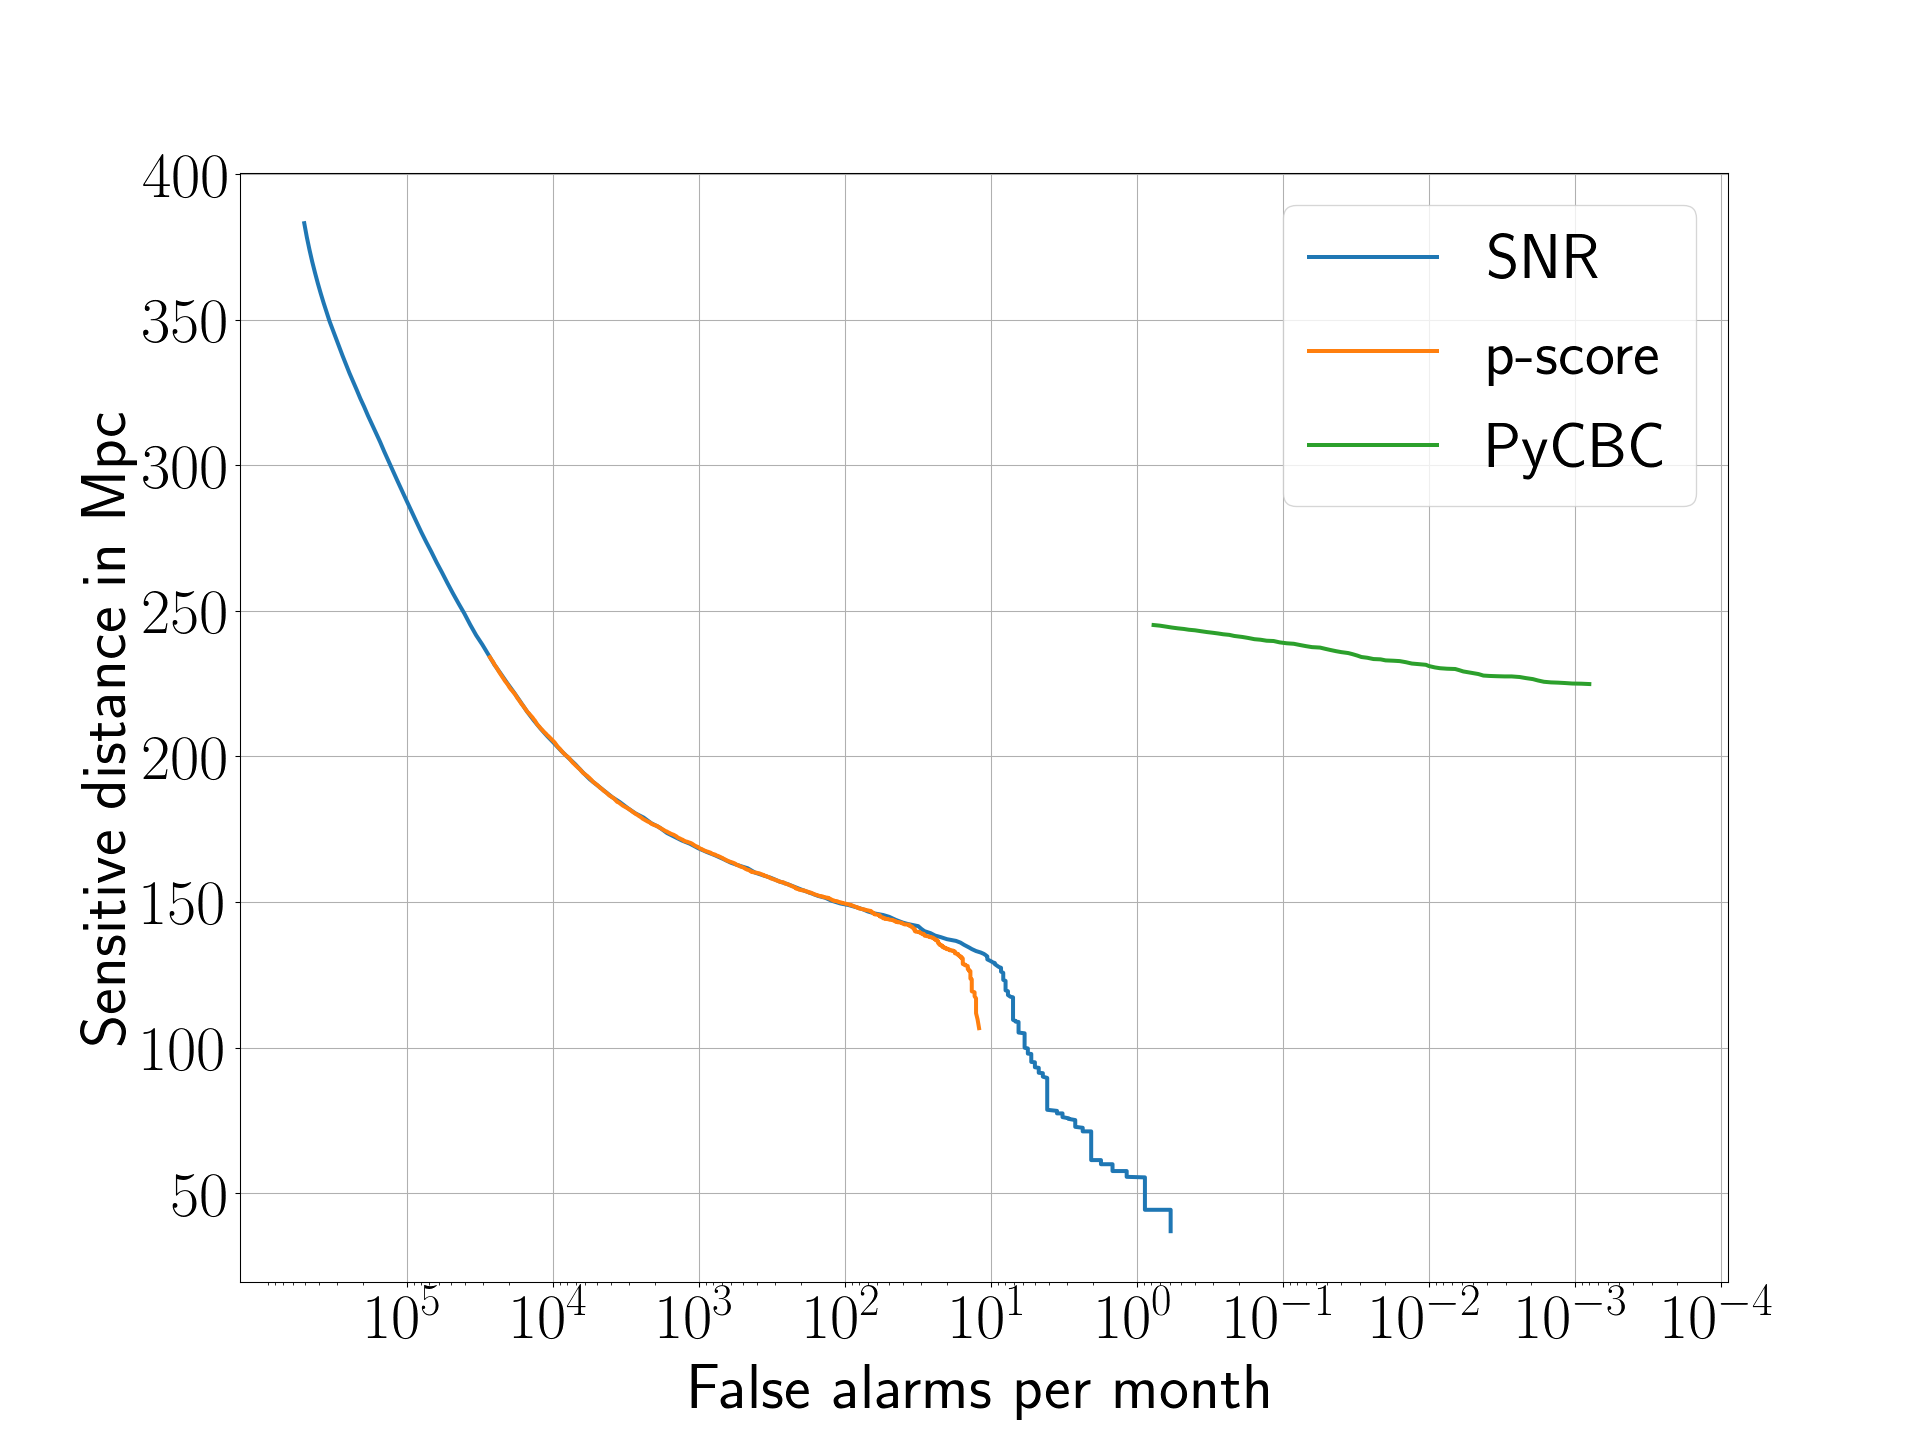
\includegraphics[width=0.8\textwidth]{chapters/bnsnet/images/SensitivitySNR}
	\caption[Sensitivity]{The sensitive distance as a function of the \acrshort{far}. The blue curve shows the sensitive distance when the \acrshort{snr} is used to classify events. The yellow curve shows the sensitive distance when the p-score is used. The green curve is generated from the data found in \cite{Nitz:2017svb} by counting all signals at a higher injection \acrshort{snr} than the corresponding \acrshort{far}. We are able to resolve a small overlap-region between the two different searches but find that the sensitivity of our search drops close to zero for \acrshort{far}s below 10 per month. At high \acrshort{far}s both outputs of our network perform equally well, for low \acrshort{far}s the \acrshort{snr} shows superior performance. Figure and caption were taken from \cite{Schafer:2020kor}.}\label{fig:bns_sensitivity}
\end{figure}

We compare our analysis to PyCBC Live~\cite{Nitz:2018rgo}. To estimate the sensitivity of PyCBC Live, we use Figure 1 from \cite{Nitz:2017svb} to obtain a ranking statistic $\mathcal{R}$ as a function of \acrshort{far}. We then assume that all injections with optimal network \acrshort{snr} $> \mathcal{R}$ are found by PyCBC Live. The green curve in \autoref{fig:bns_sensitivity} shows the resulting sensitivity curve. We find that PyCBC Live achieves about twice the sensitive distance measured for our algorithm at a \acrshort{far} lower by about one order of magnitude. We also measure the latency introduced by our algorithm to compare it to the latency of PyCBC live. Ignoring pre-processing, our algorithm is capable of producing alerts in real time and introduces an average latency of \SI{10.2}{\second}. Restricting PyCBC Live to the parameter region of \autoref{tab:bns_parameter_distribution} results in a template bank containing $1960$ templates per detector, which can be used to filter the data for both detectors on a single \acrshort{cpu} core in real time. This analysis also introduces a latency of $\mathcal{O}(10)$ seconds, making it at least as computationally efficient as our deep learning alternative.

We also compare our search algorithms to another deep learning based \acrshort{bns} signal detection pipeline published as \cite{Krastev:2019koe}. The original pre-print \cite{Krastev:2019aaa} was revised before publication as \cite{Krastev:2019koe} shortly before we published our study. For this reason we compare our approach to both versions. The pre-print study~\cite{Krastev:2019aaa} gave signal strength in terms a peak signal-to-noise ratio (\acrshort{psnr}), which we estimate to be related to optimal \acrshort{snr} by $\text{\acrshort{snr}}=41.2\text{\acrshort{psnr}}$. Both the pre-print as well as the published version operate only on data from a single detector, whereas our algorithm uses data from two detectors. For this reason, we also scale the \acrshort{snr} from \cite{Krastev:2019aaa} and \cite{Krastev:2019koe} by a factor of $\sqrt{2}$ to estimate the network \acrshort{snr}. The comparison in terms of true positive rate can be found in \autoref{fig:bns_tpr} at different \acrshort{far}s. We find that our approach is about $4$ times as sensitive as the one presented in \cite{Krastev:2019koe} in the \acrshort{snr} region our network was trained on, which is marked by the gray area in the plot. However, our algorithm falls off rapidly for loud signals and only saturates at a sensitivity of $100\%$ for \acrshort{snr}s $>46.65$.
\begin{figure}
	\centering
	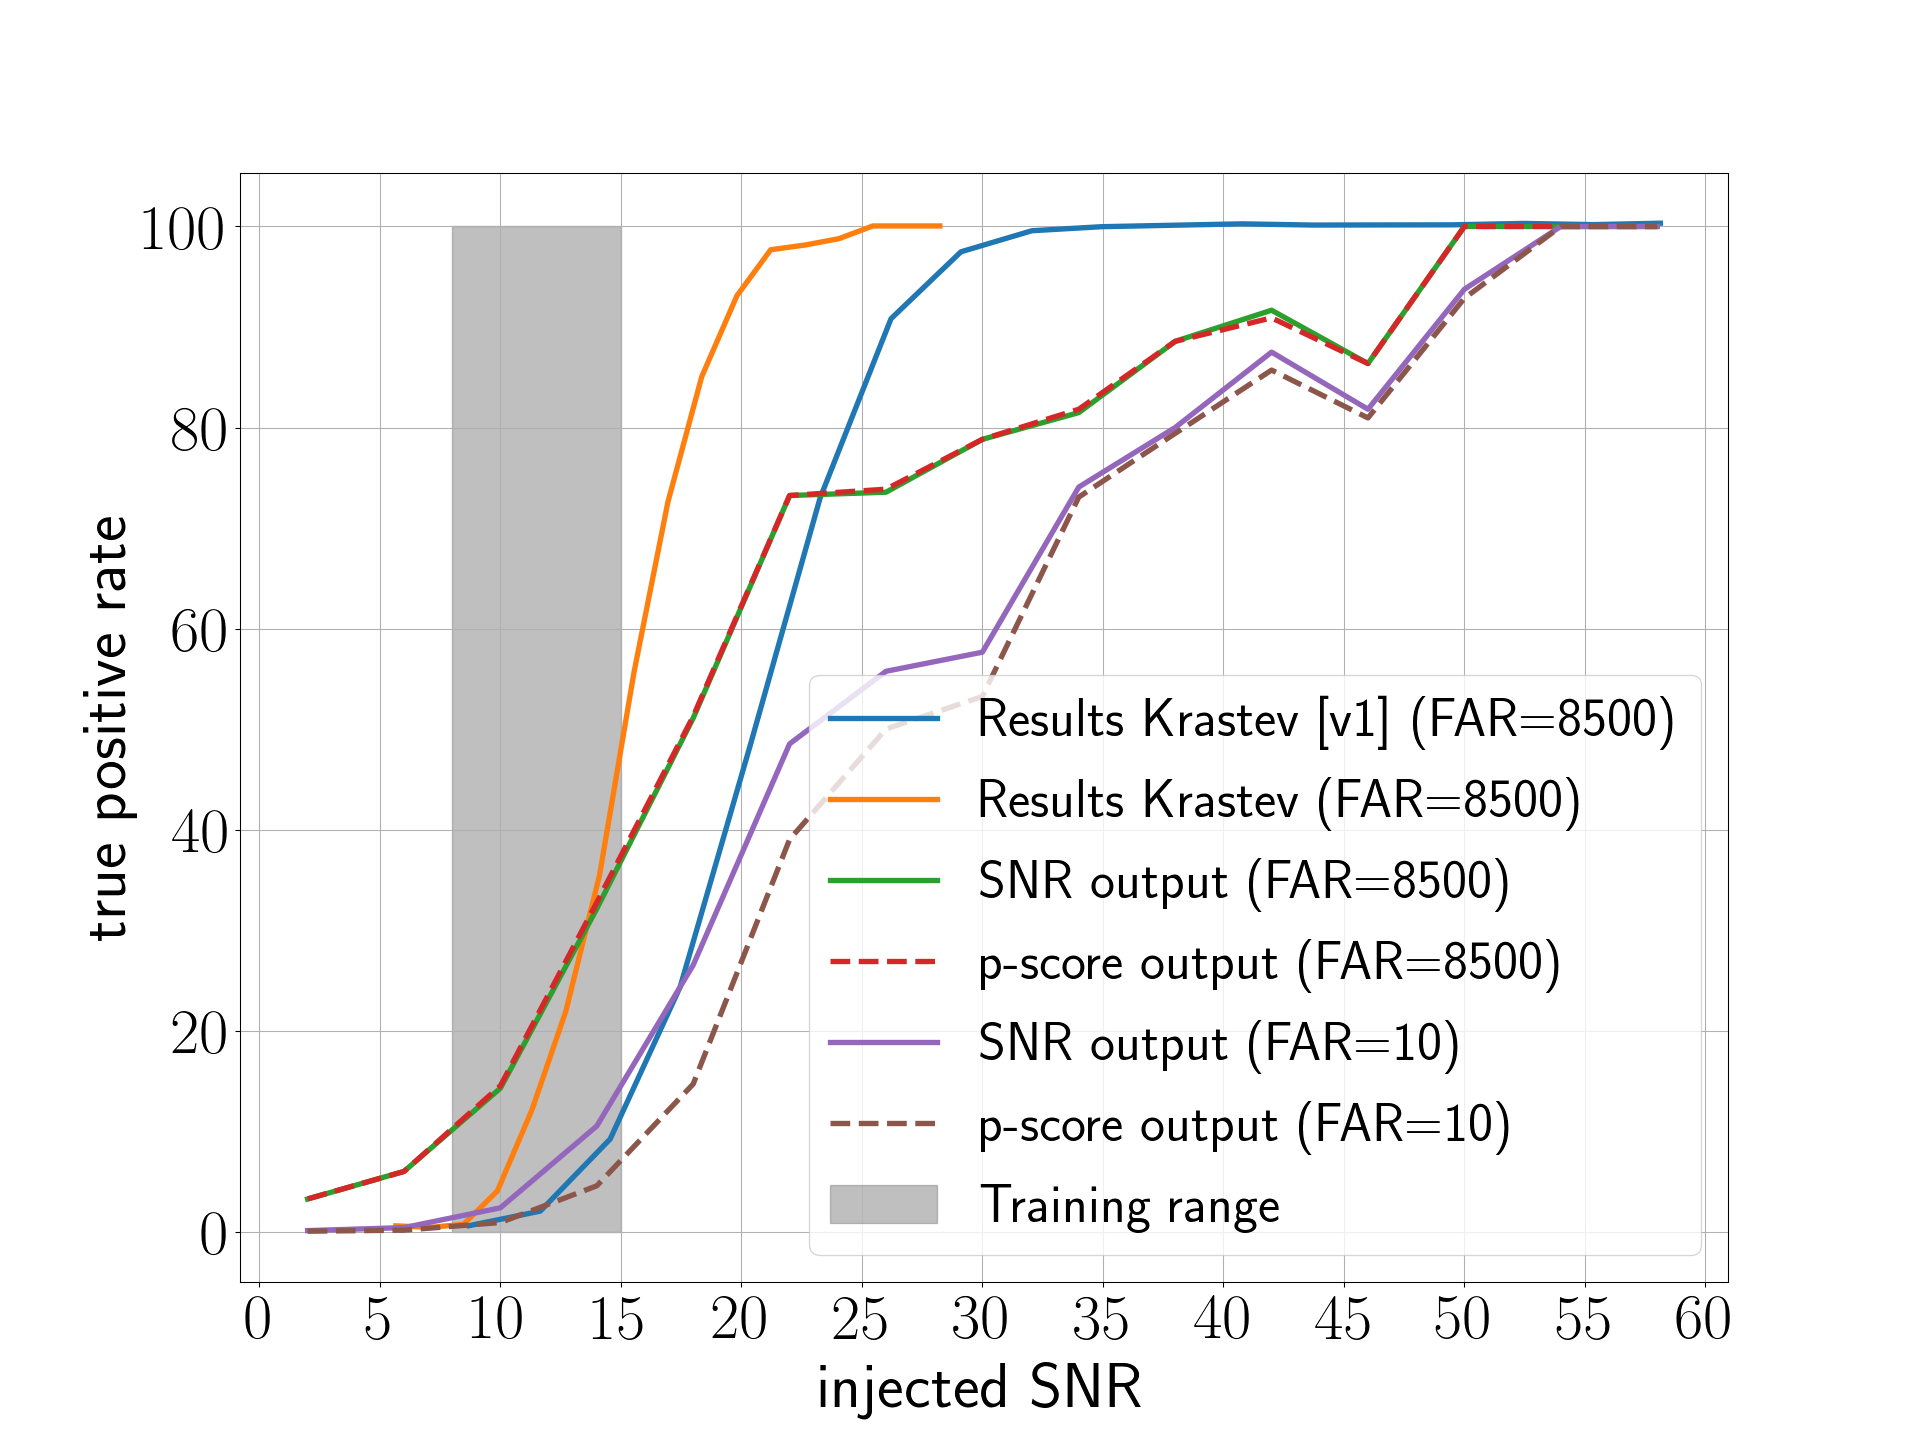
\includegraphics[width=0.8\textwidth]{chapters/bnsnet/images/compare_krastev_v2}
	\caption[True positive rate]{To compare our search to the work of \cite{Krastev:2019koe} we plot their true positive rate at a fixed \acrshort{far} of $8500$ per month in yellow and our true positive rate at the same \acrshort{far} in green and red. On the x-axis we track the injected optimal network \acrshort{snr}. The blue curve shows the data from \cite{Krastev:2019aaa}, where the results were given in terms of pSNR. We use the conversion $\text{\acrshort{snr}} = 41.2\cdot\sqrt{2}\cdot\text{pSNR}$. To obtain these curves we bin the injected signals by their optimal injection \acrshort{snr} and a bin size of 4. For high \acrshort{snr}s some bins are empty. Empty bins are interpolated linearly from the remaining data. The area marked gray highlights the region covered by the training set. We find that our search performs better for low \acrshort{snr}s but is less sensitive for strong signals. We also show the true positive rate of our search at a \acrshort{far} of 10 in purple and brown. Within the training range we find that our search closely matches the true positive rate of \cite{Krastev:2019aaa} at a higher \acrshort{far}. Figure and caption were taken from \cite{Schafer:2020kor}.}\label{fig:bns_tpr}
\end{figure}

\section{Conclusions}
We introduced a novel procedure of making long duration time domain data accessible to \acrshort{nn}s, by sampling the data at multiple rates. This multi-rate sampling was used to train and evaluate a deep learning based search algorithm for \acrshort{gw}s from \acrshort{bns} mergers. We compared it to the state-of-the-art matched filter based low-latency search pipeline PyCBC Live and found that it is neither computationally more efficient nor as sensitive. This shows that more work is required to build competitive deep learning search algorithms for complex signals.

We also compare our analysis to another deep learning \acrshort{bns} search algorithm. Our algorithm was approximately four times as sensitive to signals with \acrshort{snr} $\leq 15$ but could not generalize well to louder signals.

Finally, we proposed an evaluation scheme that produces results that are comparable to existing pipelines and is normalized to the injected population of \acrshort{gw} sources. We used this scheme to test our algorithm down to a \acrshort{far} of $0.3$ per month. This analysis showed that the sensitivity of our deep learning based algorithm drops to zero for \acrshort{far}s that are low compared to \acrshort{far}s at which deep learning algorithms are usually tested. Following \cite{Gebhard:2019ldz}, we argued that using \acrshort{fap}s, which are derived on discrete samples does not translate well to performance measures based on the more physically relevant \acrshort{far}s, as clustering effects are disregarded for \acrshort{fap}s.


\chapter{Gravitational-wave Merger Forecasting: Scenarios for the Early Detection and Localization of Compact-binary Mergers with Ground-based Observatories}\label{ch:forecasting}
\chaptermark{Gravitational-wave Merger Forecasting}
This chapter summarizes the work published as \cite{Nitz:2020vym}. It discusses a classical low-latency search for pre-merger detection of \acrshort{bns} systems. It is covered in this thesis, as machine learning is often stated to be a tool to decrease latency. Having a reference point of existing algorithms that are capable of pre-merger detection is important to determine research areas where machine learning algorithms may be of practical use.

\section{Introduction}
GW170817~\cite{LIGOScientific:2017vwq} was the first detected \acrshort{gw} event emitted by a \acrshort{bns} merger. It was accompanied by an \acrshort{em} counterpart observed in multiple frequency bands~\cite{LIGOScientific:2017ync}. The earliest \acrshort{em} signal was a gamma ray burst observed by Fermi-GBM and INTEGRAL~\cite{Goldstein:2017mmi, Savchenko:2017ffs, Monitor:2017mdv} about \SI{1.7}{\second} after the \acrshort{gw} merger. The first optical observations began only about $11$ hours after the merger~\cite{Coulter:2017wya}. These \acrshort{em} observations provided new insight into the nuclear equation of state~\cite{LIGOScientific:2018hze, LIGOScientific:2018cki, Radice:2017lry, Kiuchi:2019lls, Capano:2019eae, LIGOScientific:2019eut}, the Hubble constant~\cite{Guidorzi:2017ogy, Hotokezaka:2018dfi, LIGOScientific:2018gmd}, the phenomenon of kilonova (see ~\cite{Metzger:2019zeh} and references therein), and the central engine of short gamma-ray bursts~\cite{Murguia-Berthier:2020tfs, Wu:2019rla, Lazzati:2020vbo, Nitz:2020vym}.

If early observations of the optical band would have been available, different kilonova emission models could have been differentiated~\cite{Arcavi:2018mzm}. It is also hypothesisized that pre-merger \acrshort{em} emissions exist~\cite{Hansen:2000am, Troja:2010zm, Tsang:2011ad, Metzger:2016mqu, Wang:2016dgs, Wada:2020kha}, which could be constrained by pre-merger observations. However, early or even pre-merger \acrshort{em} observation of \acrshort{cbc} mergers are constrained by two factors: The latency between \acrshort{gw} signal detection and telescopes being alerted, as well as the ability of \acrshort{em} instruments being able to cover the sky area where the source is estimated to be located.

This study assesses the possibility of generating pre-merger alerts for different eras of detectors and quantifies the localization error associated with them. By providing pre-merger alerts, the latency is automatically reduced. Quantifying the localization error allows for \acrshort{em} observation strategies to be optimized and coordinated. To do so, the evolution of the pre-merger alert capabilities of ground based detectors over the next $\mathcal{O}(10)$ years are evaluated. Additionally, the capabilities of the current low-latency PyCBC Live~\cite{Nitz:2018rgo, DalCanton:2020vpm} analysis to generate early warnings is tested.

\section{Methods}
Our study covers the five current and planned ground based \acrshort{gw} observatories of the coming decade \acrshort{ligo}-Hanford (H), \acrshort{ligo}-Livingston (L)~\cite{LIGOScientific:2014pky}, \acrshort{ligo}-India (I)~\cite{Iyer:2011aaa}, Virgo (V)~\cite{VIRGO:2014yos}, and KAGRA (K)~\cite{KAGRA:2018plz}. For this network of detectors, we consider three different eras: ``Design'', ``A+'', and ``Voyager''. The ``Design'' era expects the four detectors \acrshort{ligo}-Hanford, \acrshort{ligo}-Livingston, Virgo, and KAGRA to be operational at their 2021-2022 design sensitivity~\cite{KAGRA:2013rdx}. Starting with the ``A+'' era, we expect \acrshort{ligo}-India to be operational and matching the sensitivity of both \acrshort{ligo}-Hanford and \acrshort{ligo}-Livingston. We use the design \acrshort{psd} of the planned upgrades to the \acrshort{ligo} instruments from 2024-2026 for the three \acrshort{ligo} detectors~\cite{Barsotti:2018aaa}. For Virgo and KAGRA we conservatively assume that their sensitivity will not improve beyond their ``Design'' era. The ``Voyager'' era assumes the \acrshort{psd} of the three \acrshort{ligo} detectors to match the ``Voyager'' plans~\cite{LIGOScientific:2017aaa}. A follow-up study covered the third generation detectors \acrshort{et} and \acrshort{cw}~\cite{Nitz:2021pbr}.

To assess the capability of pre-merger detection in the different configurations discussed in \cite{Nitz:2020vym}, we simulated a population of $\mathcal{O}(10^5)$ \acrshort{bns} mergers. This population is distributed uniformly in volume and isotropically in sky location and binary orientation. The masses are chosen to be a reference binary with \SI[parse-numbers=false]{1.4-1.4}{M_\odot}, but the results can be generalized to arbitrary masses (see Section 4 in \cite{Nitz:2020vym}). The signals are subsequently injected into simulated, Gaussian noise, colored by the \acrshort{psd} of different detectors and eras.

We pursue two different criteria for signal detection. To gauge the general capability of pre-merger detection, our first method assumes the detection of a signal if the combined optimal network \acrshort{snr} $> 10$. This choice is consistent with the threshold for confidently detected mergers in~\cite{LIGOScientific:2018mvr, Nitz:2020oeq}. To determine the pre-merger detection capabilities, we calculate the network \acrshort{snr} as a function of time before merger. Once the network \acrshort{snr} exceeds the threshold, it is counted as detected and we generate a posterior of the sky location using Baystar~\cite{Singer:2015ema} for every time step. The second method involves a full search using PyCBC Live in a low-latency configuration at a \acrshort{far} of $1$ per year. To adapt it to pre-merger detection, the template bank is a combination of several template banks using different pre-merger truncation times. The truncation of the different banks are chosen such that they cover $5\%$ increments of the total expected \acrshort{snr}. This second analysis allows us to test how capable existing analysis methods are at pre-merger detection. Sky localization is again performed using Baystar~\cite{Singer:2015ema}.

\section{Results}
The core results of the study are given in Figures \ref{fig:res_design} to \ref{fig:res_voyager}. They show the search sensitivity, localization error accuracy, and detection rate estimates as functions of time of detection before merger. The two columns compare the network of currently operational detectors with the planned detector network for each era. The times on the horizontal axis do not include the latency of the analysis or any other processing. They merely reflect the upper frequency cutoff at which the two analysis methods can detect them.
\begin{figure}
	\centering
	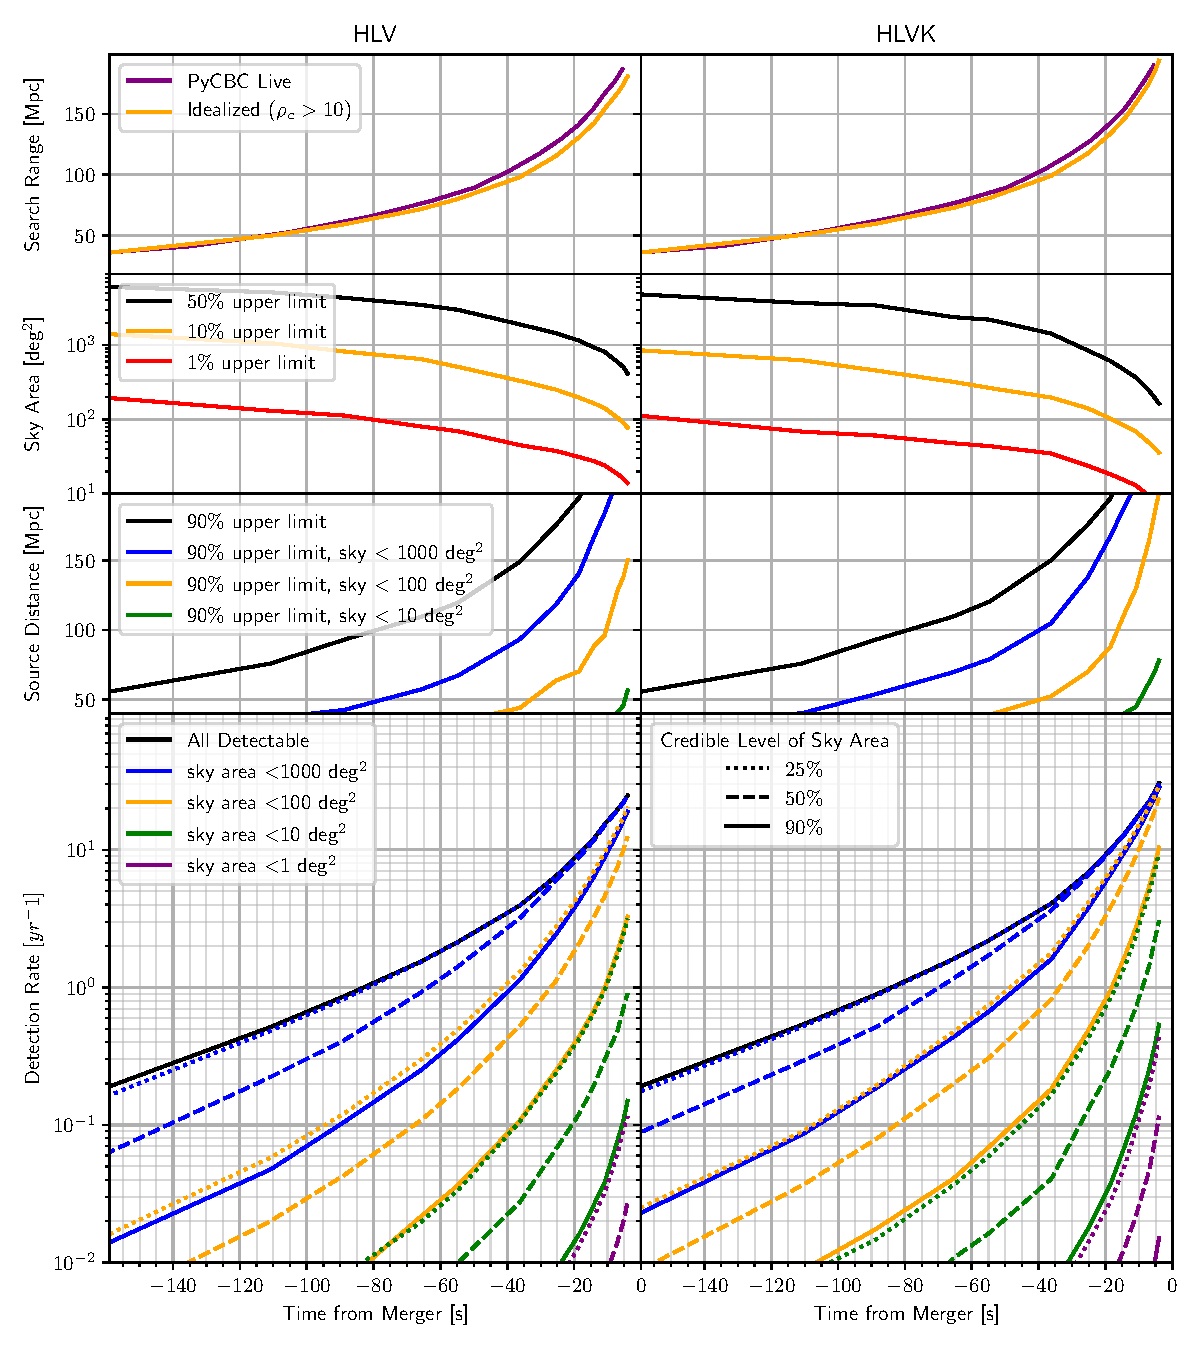
\includegraphics[width=\textwidth]{chapters/forecasting/images/design.pdf}
	\caption[``Design'' era detection ranges, localizations, distances, and merger rates]{``Design'' era (2021-2022) detection and localization for the HLV network (left) and the full gravitational-wave detector network (right) as a function of time before merger for a fiducial 1.4-1.4$M_\odot$ BNS merger. (Top) The sky-averaged detection range for the idealized search and PyCBC Live operating at a false alarm rate of once per year. (Middle) The upper limit on the localization sky area and source distance, respectively, for detectable sources. Sky areas are quoted at the 90$\%$ credible level. (Bottom) The detection rate of all sources (black) and those that also have a sky localization less than 1000 deg$^2$ (blue), 100 deg$^2$ (orange), 10 deg$^2$ (green), or 1 deg$^2$ at a 90$\%$ (solid), 50$\%$ (dashed), and 25$\%$ credible level (dotted). Figure and caption are taken from \cite{Nitz:2020vym}.}\label{fig:res_design}
\end{figure}
\begin{figure}
	\centering
	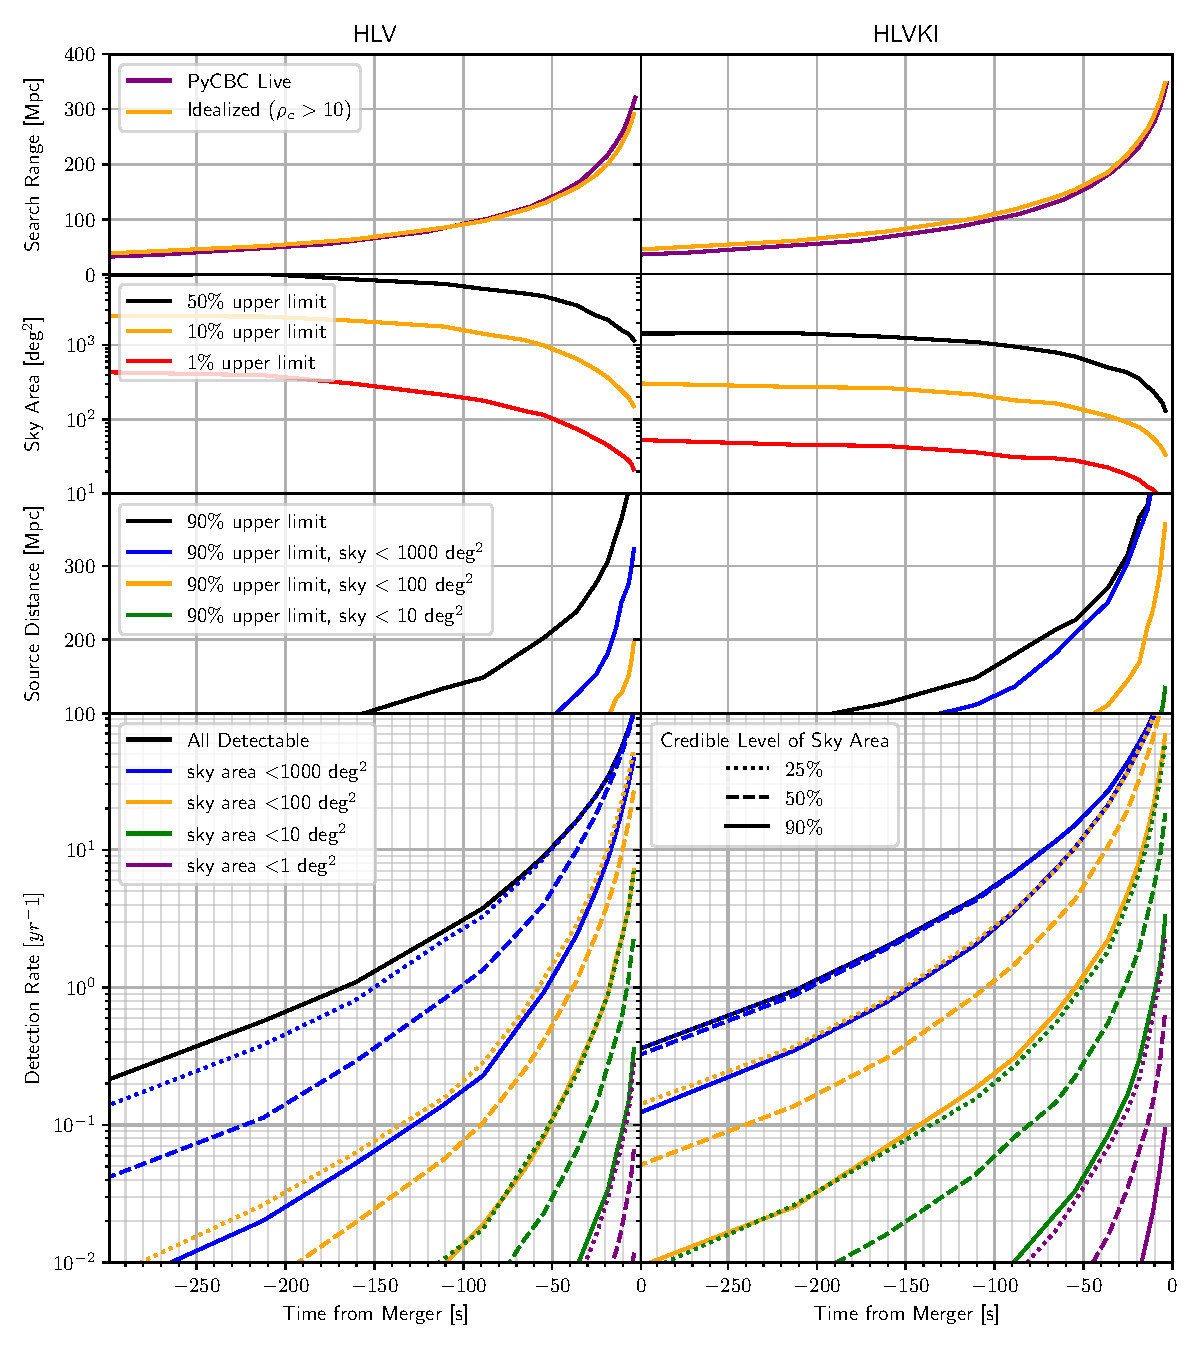
\includegraphics[width=\textwidth]{chapters/forecasting/images/aplus.pdf}
	\caption[``A+'' era detection ranges, localizations, distances, and merger rates]{``A+'' era (2024-2026)  detection and localization for the HLV network (left) and the full gravitational-wave detector network (right) as a function of time before merger for a fiducial 1.4-1.4$M_\odot$ BNS merger. (Top) The sky-averaged detection range for the idealized search and PyCBC Live operating at a false alarm rate of once per year. (Middle) The upper limit on the localization sky area and source distance, respectively, for detectable sources. Sky areas are quoted at the 90$\%$ credible level. (Bottom) The detection rate of all sources (black) and those that also have a sky localization less than 1000 deg$^2$ (blue), 100 deg$^2$ (orange), 10 deg$^2$ (green), or 1 deg$^2$ at a 90$\%$ (solid), 50$\%$ (dashed), and 25$\%$ credible level (dotted). Figure and caption are taken from \cite{Nitz:2020vym}.}\label{fig:res_aplus}
\end{figure}
\begin{figure}
	\centering
	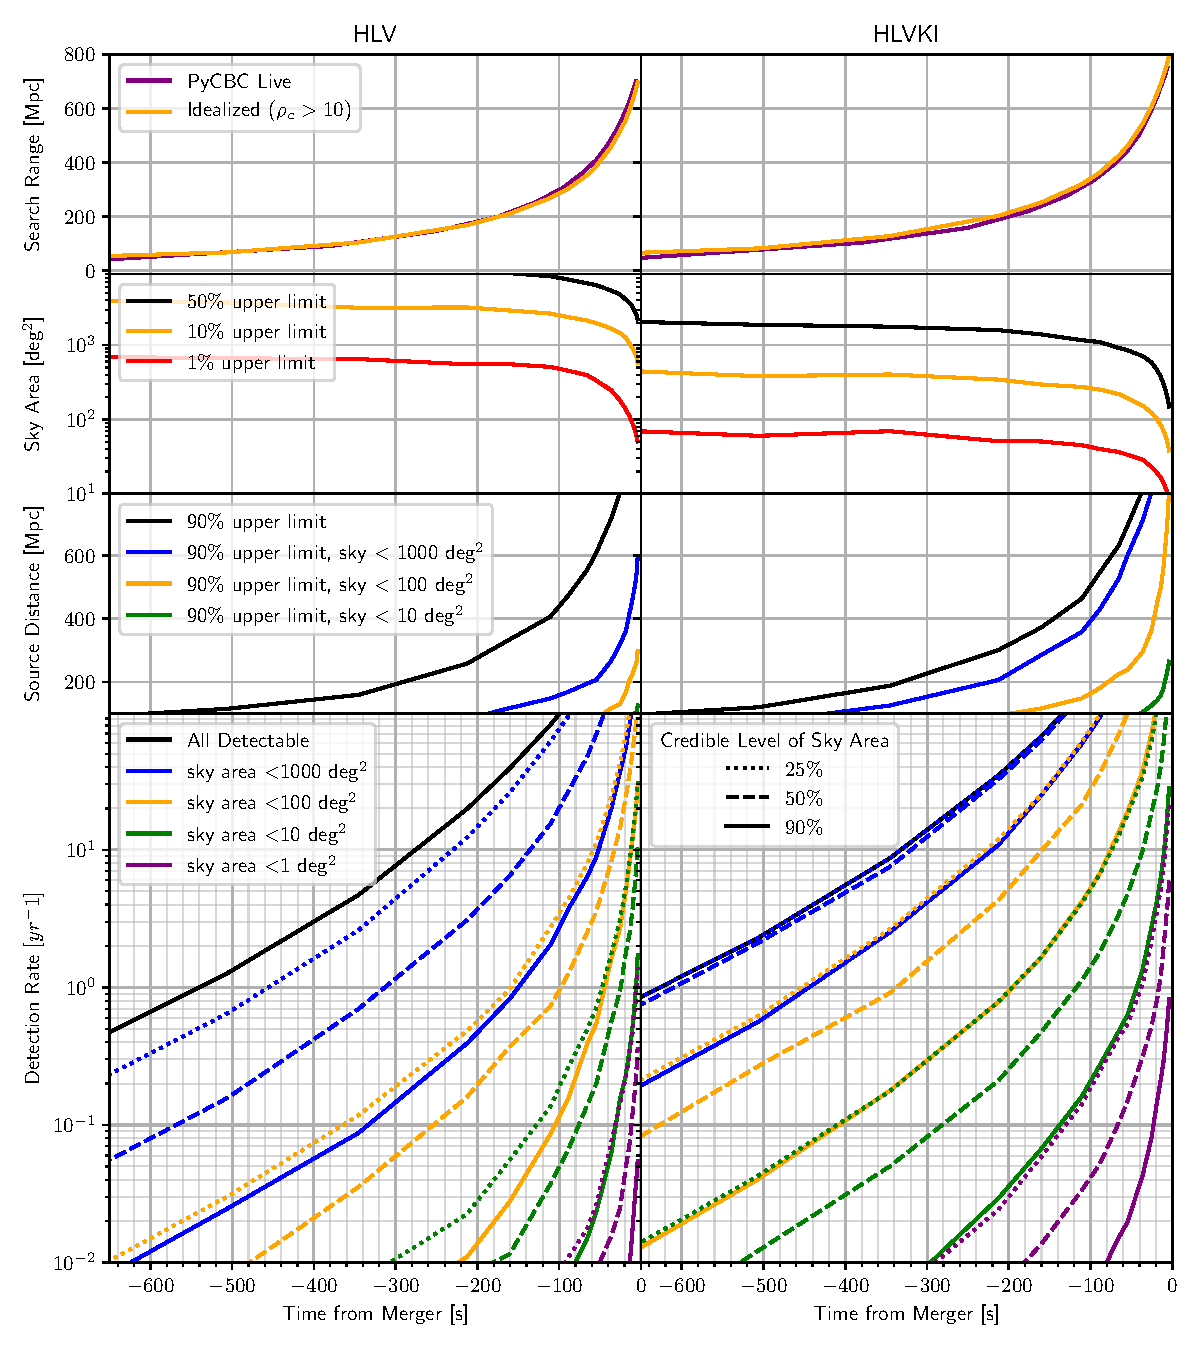
\includegraphics[width=\textwidth]{chapters/forecasting/images/voyager.pdf}
	\caption[``Voyager'' era detection ranges, localizations, distances, and merger rates]{``Voyager'' era (late 2020's)  detection and localization for the HLV network (left) and the full gravitational-wave detector network (right) as a function of time before merger for a fiducial 1.4-1.4$M_\odot$ BNS merger. (Top) The sky-averaged detection range for the idealized search and PyCBC Live operating at a false alarm rate of once per year. (Middle) The upper limit on the localization sky area and source distance, respectively, for detectable sources. Sky areas are quoted at the 90$\%$ credible level. (Bottom) The detection rate of all sources (black) and those that also have a sky localization less than 1000 deg$^2$ (blue), 100 deg$^2$ (orange), 10 deg$^2$ (green), or 1 deg$^2$ at a 90$\%$ (solid), 50$\%$ (dashed), and 25$\%$ credible level (dotted). Figure and caption are taken from \cite{Nitz:2020vym}.}\label{fig:res_voyager}
\end{figure}

From the plots, we find that the PyCBC Live analysis is comparable to the idealized search and even outperforms it at a \acrshort{far} of 1 per month. This shows that current analysis methods are fully capable of pre-merger detections at the calculated rates. Assuming a merger rate density of \SI{1000}{\giga\parsec^{-3}\years^{-1}}, we find that one source per year can be expected to be detected with a $90\%$ confidence localization of $<100$~deg$^2$ and an early warning of \SI{18}{\second}, \SI{54}{\second}, and \SI{195}{\second} for the ``Design'', ``A+'', and ``Voyager'' era, respectively. If the confidence region is reduced to $50\%$, the early warning increases to \SI{34}{\second}, \SI{104}{\second}, and \SI{335}{\second}. Alternatively, the pre-merger warning can be kept constant to increase the expected number of detections to $4-6$ sources per year. This strategy would more than double the number of detected \acrshort{em} counterparts, assuming that $50\%$ of the counterparts lie outside the credible region.
\newpage

\section{Conclusions}
We have shown that for different detector network configurations in the coming decade the possible pre-warning time for a \acrshort{bns} merger may increase from $\mathcal{O}\lr{10}$ to $\mathcal{O}\lr{100}$ seconds. However, this amount of pre-warning is still insufficient for many observatories for re-pointing and tiling a $100$ deg$^2$ area~\cite{Coughlin:2019qkn}. Notable exceptions include Swift~\cite{Tohuvavohu:2020stm}, ZTF~\cite{Bellm:2018aaa, Coughlin:2019xfb}, MASTER~\cite{Kornilov:2011fi}, and CTA~\cite{CTAConsortium:2013ofs}. Observatories that are not capable of re-point and tile the sky region in the provided early warning time may still benefit by adjusting their observing configurations~\cite{James:2019xca}.

We hope that this roadmap provides grounds for the observing community to plan continued and automated observations with existing instruments, as well as further motivation to build new instruments with different observation bands. This includes concepts such as the Transient Astrophysics Probe~\cite{Camp:2019aaa}. If these hopes are met, it seems plausible that the first \acrshort{bns} detection with simultaneous observation of the prompt \acrshort{em} emissions can be made within the next decade. 


\chapter{Training Strategies for Deep Learning Gravitational-Wave Searches}\label{ch:training_strats}
\minitoc
This chapter is essentially a full reprint of \cite{Schafer:2021fea} with minor edits for formatting. It discusses the influence of different training strategies on deep learning \acrshort{gw} search algorithms and introduces a novel way of treating the network output. 

\setcounter{section}{-1}
\section{Abstract}
Compact binary systems emit gravitational radiation which is potentially detectable by current Earth bound detectors. Extracting these signals from the instruments' background noise is a complex problem and the computational cost of most current searches depends on the complexity of the source model. Deep learning may be capable of finding signals where current algorithms hit computational limits. Here we restrict our analysis to signals from non-spinning binary black holes and systematically test different strategies by which training data is presented to the networks. To assess the impact of the training strategies, we re-analyze the first published networks and directly compare them to an equivalent matched-filter search. We find that the deep learning algorithms can generalize low signal-to-noise ratio (\acrshort{snr}) signals to high \acrshort{snr} ones but not vice versa. As such, it is not beneficial to provide high \acrshort{snr} signals during training, and fastest convergence is achieved when low \acrshort{snr} samples are provided early on. During testing we found that the networks are sometimes unable to recover any signals when a false alarm probability $<10^{-3}$ is required. We resolve this restriction by applying a modification we call unbounded Softmax replacement (\acrshort{usr}) after training. With this alteration we find that the machine learning search retains $\geq 91.5\%$ of the sensitivity of the matched-filter search down to a false-alarm rate of $1$ per month.

\section{Introduction}
The direct detection of a gravitational wave (\acrshort{gw}) on September 14, 2015 \cite{LIGOScientific:2016aoc} started the era of \acrshort{gw} astronomy. After the analysis of two and a half observing runs, tens of \acrshort{gw}s have been confirmed \cite{LIGOScientific:2020ibl, Nitz:2021uxj}. GW170817 \cite{LIGOScientific:2017vwq} was the first \acrshort{gw} event also seen in the electromagnetic spectrum \cite{Goldstein:2017mmi, Savchenko:2017ffs, DES:2017kbs, LIGOScientific:2017ync}.

The latency between a \acrshort{gw} and its reported detection is a vital aspect of multi-messenger missions. Lowering the delay between data aggregation and signal detection allows to maximize the electromagnetic observation time and reduces the risk that early emissions are being missed.

To extract \acrshort{gw} signals from the instrument data, a well-established technique known as \textit{matched filtering} is used in many search algorithms. It convolves \textit{templates}, i.e.\ pre-calculated models of the expected signals, with the measured data \cite{ligo_pipelines, Sachdev:2019vvd, Adams:2015ulm, Nitz:2018rgo, Hooper:2011rb}. When one of these templates matches the data to a given degree and the data quality is high enough, these searches report a candidate detection. 

Matched filtering is known to be optimal in stationary Gaussian noise when accurate models of the waveform exist~\cite{Allen:2005fk}. However, it can be computationally limiting when many templates are required. This is the case when effects such as higher-order modes \cite{Harry:2017weg}, precession \cite{Harry:2016ijz} or eccentricity \cite{Nitz:2019spj} are considered. Furthermore, signals which are not covered by the filter bank may be missed entirely. While there are unmodeled searches that detect coincident excess power in different detectors \cite{Klimenko:2005xv, Klimenko:2015ypf, Lynch:2015yin}, they are less sensitive in regions where accurate models exist.

Recently, new deep learning based searches have started to be explored \cite{George:2016hay, George:2017pmj, Gabbard:2017lja, Dreissigacker:2019edy, Krastev:2019koe, Schafer:2020kor}. Summaries of the current state of the field are given in \cite{Cuoco:2020ogp, Huerta:2021ybd}. The pioneering works by George et al.\ \cite{George:2016hay} and Gabbard et al.\ \cite{Gabbard:2017lja} demonstrated that deep neural networks are capable of detecting \acrshort{gw}s from two merging black holes (\acrshort{bbh}). The networks have also proven to generalize to signals with previously unseen parameters \cite{George:2016hay, Xia:2020vem}. It was shown that these algorithms can distinguish data containing a \acrshort{gw} from pure noise as well as matched filtering with a false-alarm probability (\acrshort{fap}) down to $10^{-3}$. That means, the networks were tested down to a level at which about 1 in 1000 pure noise samples was falsely classified as containing a signal.

The authors of \cite{Gebhard:2019ldz} find that the \acrshort{fap}s determined by the original studies do not directly translate to false-alarm rates (\acrshort{far}s) on continuous data streams. For \acrshort{far}s, the appropriate question to ask is how many false signals does the network identify per time interval of continuous data, as opposed to how many uncorrelated data chunks are falsely identified as containing a signal. The effects of clustering subsequent outputs when the network is applied via a sliding window have to be accounted for. Comparing deep learning searches to traditional matched-filter searches is, therefore, not trivial because matched-filter searches typically operate at \acrshort{far}s that are orders of magnitude smaller than what has been tested for early neural networks. In \cite{Schafer:2020kor} we suggested a standardized testing procedure which produces statistics which are comparable to traditional search algorithms to resolve these issues.

In this paper we reanalyze and extend the results given in the initial papers \cite{George:2016hay, Gabbard:2017lja}. Our motivation is twofold. First, we want to verify and test the performance of the networks quoted in those papers. Specifically, we apply the testing procedure outlined in \cite{Schafer:2020kor}. Second, we discuss how the \acrshort{gw} data is prepared for and presented to the network. The form of data preparation is often taken as a given, while comparatively more work is invested in finding a network structure that suits the problem. We carefully examine the influence of different choices of data presentation and training strategies on the ability to detect signals given a fixed network.

Here we focus on signal detection. The problem of deep learning parameter estimation is another vital and active area of research. Multiple groups have made advancements in this field \cite{Chua:2019wwt, Gabbard:2019rde, Green:2020hst, Williams:2021qyt, Schmidt:2020yuu, George:2016hay}.

We use the network presented by Gabbard et al.\ \cite{Gabbard:2017lja} for most of our studies. It is trained on simulated data containing \acrshort{gw}s from \acrshort{bbh}s with individual black hole masses ranging from \SIrange{10}{50}{M_\odot}. The search is restricted to a single detector. This restriction reduces the parameter space to the two component masses, the orbital phase, the distance to the source and the time of coalescence.

The network classifies segments of \SI{1}{\second} duration sampled at \SI{2048}{\hertz} into the two categories ``$\text{noise}+\text{signal}$'' and ``noise'' by returning a value between 0 and 1 we call ``p-score''. A larger p-score corresponds to a higher confidence of the network that the input contains a signal.

To optimize the training strategy, we focus on the difference between \textit{curriculum learning} \cite{Bengio:2009aaa} and \textit{fixed interval training}. Fixed interval training uses a single training set, i.e.\ a single, fixed range of signal-to-noise ratios (\acrshort{snr}s). Curriculum learning lowers the \acrshort{snr} of the training signals progressively, thus increasing the complexity with time. We evaluate different variants of both strategies. In total 15 different approaches are tested.

Each strategy is applied to 50 randomly initialized networks. We do this to guard against favorable initializations. All tests are done with two different implementations, to further increase robustness of our results. The different implementations use the two core libraries Tensorflow \cite{Abadi:2015aaa} and PyTorch \cite{Paszke:2019aaa}, respectively.

We find that most training strategies are capable of closely reproducing the results given in \cite{Gabbard:2017lja}. We do not see a significant difference in performance between curriculum learning and fixed interval training strategies. However, networks that had access to lower \acrshort{snr} signals during training generally outperformed those that only saw high \acrshort{snr} signals. We find that networks trained on fainter signals can generalize to loud ones, while the opposite is not the case.

Further analysis of the networks showed that the efficiency, which is the fraction of correctly classified input samples containing a signal at a given \acrshort{fap}, drops to zero beyond a \acrshort{fap} of $10^{-3}$ when the training is carried out for long enough. This drop is caused by numerical instabilities in the final activation and the comparatively low penalty of false positives. We propose a simple modification that does not require retraining of the network to push this problem to significantly lower \acrshort{fap}s. We call this modification unbounded Softmax replacement (\acrshort{usr}).

We evaluate 3 different networks of each training strategy on a month of simulated data. The networks are applied using a sliding window with step size of \SI{0.1}{\second}. We follow the procedure outlined in \cite{Schafer:2020kor} to analyze the results. Our evaluation of the base line network is limited by $\mathcal{O}\left(10^3\right)$ false alarms estimated with perfect confidence to contain a signal. By applying the \acrshort{usr} modification we are able to eliminate this restriction and can calculate sensitivities down to a \acrshort{far} of $1$ per month. For comparison, we construct a template bank and use it to do a matched-filter search on the same data used to evaluate the networks. We find that the machine learning search retains at least $91.5\%$ of the sensitivity of a matched-filter search for all tested \acrshort{far}s and most strategies.

All code required to reproduce our analysis is public and can be found at \cite{ml-training-strategies-github}.

The contents of this paper are structured as follows. In \autoref{sec:train_strat_methods} we describe the architecture, data sets, training strategies, and evaluation methods. We apply these in \autoref{sec:train_strat_results} and describe our findings. In particular we describe the \acrshort{usr} modification which allows the networks to be tested at low \acrshort{fap}s. We conclude in \autoref{sec:conclusion}.


\section{Methods}\label{sec:train_strat_methods}

\subsection{General setup}\label{sec:methods:general}
We focus our studies on the network presented by Gabbard et al.\ in \cite{Gabbard:2017lja}. They used a convolutional neural network with 6 stacked convolutional layers followed by 3 fully connected layers. All but the last layer use an exponential linear unit (\acrshort{elu}) as activation function.

The architecture is altered in two details compared to the original version of \cite{Gabbard:2017lja}. We added a batch normalization layer before the first convolutional layer to take care of \textit{input normalization}. Input normalization scales all inputs to have a mean-value of 0 and a variance of 1. This is standard practice in contemporary deep learning and has been proven to help the network train efficiently \cite{Ioffe:2015aaa}. The second modification is a reduction of the pool sizes. This change was required because we lowered the sample rate of the data from \SI{8192}{\hertz} to \SI{2048}{\hertz}. We decided to lower the sample rate for multiple reasons. First of all, the detector sensitivity drops sharply above \SI{1}{\kilo\hertz}. Thus little to no \acrshort{snr} is lost by disregarding higher frequencies. For this reason current searches are often limited to the same frequency band as well \cite{Nitz:2018rgo, LIGOScientific:2020lst, LIGOScientific:2015kgh}. Second, signals within our training set merge at much lower frequencies and do not exceed \SI{1}{\kilo\hertz}. Finally, as we will show in \autoref{sec:train_strat_results}, our training converged to the same state as previous works. We are thus confident that this reduction in the sample rate has no negative impact on the network's ability to detect signals. A reduction of the size of the input to a neural network usually also helps with training. The resulting network setup is depicted in Table \ref{tab:train_strat_network}.

\begin{table}[]
    \caption[Network architecture]{\label{tab:train_strat_network} The modified neural network from \cite{Gabbard:2017lja} as used in this study. The given shapes correspond to the tensor shapes in the TensorFlow version of the code, i.e.\ data length $\times$ number of channels. PyTorch swaps these dimensions. The order of the layers is given by reading the column ''layer type'' from top to bottom and left to right. Layers are grouped by their influence on the output shape and by trainable weights.
    }
    \centering
    \begin{tabular}{lrr}
    	\hline\hline
	    layer type & kernel size & output shape \\
	    \hline
	    Input + BatchNorm1d & & $2048\times 1$ \\
	    Conv1D + ELU & 64 & $1985\times 8$ \\
	    Conv1D & 32 & $1954\times 8$ \\
	    MaxPool1D + ELU & 4 & $488\times 8$ \\
	    Conv1D + ELU & 32 & $457\times 16$ \\
	    Conv1D & 16 & $442\times 16$ \\
	    MaxPool1D + ELU & 3 & $147\times 16$ \\
	    Conv1D + ELU & 16 & $132\times 32$ \\
	    Conv1D & 16 & $117\times 32$ \\
	    MaxPool1D + ELU & 2 & $58\times 32$ \\
	    Flatten & & $1856$ \\
	    Dense + Dropout + ELU & & $64$ \\
	    Dense + Dropout + ELU & & $64$ \\
	    Dense + Softmax & & $2$ \\
	    \hline\hline
	\end{tabular}
\end{table}


All studies presented in \autoref{sec:methods:network_performance} and \autoref{sec:methods:training_strategies} were carried out using the network from George et al.\footnote{We adjusted the network from George et. al.\ too, by using batch normalization for input normalization and reducing the sample rate of the input to \SI{2048}{\hertz}.}\ \cite{George:2016hay} as well. However, with our particular training setup, every metric showed performance similar to the network from \cite{Gabbard:2017lja}. We present only results using the network based on the work of Gabbard et al.

Each \acrshort{gw} signal is defined by the component masses $m_1, m_2$ and a phase $\phi_0$. Two masses are drawn independently from a uniform distribution between \SI{10}{M_\odot} and \SI{50}{M_\odot} and the higher and lower values are assigned to $m_1$ and $m_2$, respectively, to enforce the condition $m_1\geq m_2$. Phases are uniformly drawn from the interval $\left[0,2\pi\right]$. We generate signals with 5 different phases for each pair of masses $\left(m_1,m_2\right)$. The amplitude, and therefore the distance of the source, is determined by the target \acrshort{snr} we have chosen. We fix the sky position to be overhead the LIGO Hanford detector \cite{LIGOScientific:2014pky} and the inclination as well as the polarization to $0$, because in the case of nonprecessing signals and assuming a single detector, any variation in those parameters can be fully absorbed by modifications of the amplitude and phase of the signal.

The waveforms are generated with a sample-rate of \SI{2048}{\hertz}, a lower-frequency cutoff of \SI{20}{\hertz}, and using the model \verb|SEOBNRv4_opt| \cite{Devine:2016ovp} (optimized version of \verb|SEOBNRv4| \cite{Bohe:2016gbl}). It is common practice to shift the location of the maximum amplitude by some small time within each training sample. This procedure allows the network to be less sensitive to the exact alignment of the waveform within its input. To achieve this behavior, we shift the position of the merger by a time uniformly drawn from \SIrange{-0.1}{0.1}{\second} before projecting onto the Hanford detector. After the projection the signals are \textit{whitened} using the analytic model of LIGO's design sensitivity at its zero detuned high power configuration \cite{lalsuite}, i.e., we divide the Fourier transformed signal by the square root of the power spectral density (\acrshort{psd}) associated with the power of the background noise at different frequencies, and transform back to the time domain. Whitening the data reduces the power at frequencies where the detector is known to be less sensitive. Next, the waveforms are scaled to an optimal \acrshort{snr} of 1. The optimal \acrshort{snr} $\rho_\text{opt}$ is defined by
\begin{equation}
    {\rho_\text{opt}}^2 = 4 \text{Re}\left[\int df \frac{\tilde{h}(f)\tilde{h}^\ast(f)}{S_n(f)}\right],
\end{equation}
where $\tilde{h}$ is the Fourier transform of the time domain signal, before it was whitened, $\tilde{h}^\ast$ is its complex conjugate, $S_n$ is the \acrshort{psd} and $\text{Re}$ extracts the real part of the complex number. Finally, we extract a time slice such that the original, not shifted merger time is located \SI{0.7}{\second} from the start of the window.

All noise is simulated from the same \acrshort{psd} used to whiten the signals. After generation, the noise is whitened by the \acrshort{psd} used to create it in the same way the signals are whitened. We choose to explicitly whiten the colored noise to take into account any artifacts the process may introduce. This also eliminates sources of errors and is in principle extendable to real noise.

The whitened signals and noise samples are combined during training. This allows us to rescale the signals at runtime to a desired strength. Since during generation all signals are scaled to \acrshort{snr} $1$, rescaling is achieved by a multiplication of the signal with the target \acrshort{snr}.

We have briefly tested training on frequency domain data. This was motivated by studies such as \cite{Dreissigacker:2019edy, Wei:2020sfz}. While these studies analyze longer duration signals, there is no conceptual problem to using the frequency representation of short \acrshort{bbh} waveforms. To accommodate the complex valued frequency representation we changed the input layer in \autoref{tab:train_strat_network} to a shape of $1025\times 2$ and inserted the real and imaginary parts as different channels. With this being our only modification to the architecture, the network was able to differentiate data containing a signal from pure noise but found up to $65\%$ fewer signals at low \acrshort{snr}. We suspect that with greater effort in finding an optimized architecture, one could regain the performance of the network on time domain data.

We have also explored training on raw data, i.e.\ data where the computationally expensive whitening is skipped. Even after several hundred epochs the network was not able to distinguish data containing signals from pure noise, irrespective of using the time or frequency domain representation of the data.

Our training set contains $20\,000$ unique combinations of component masses each of which is used to generate 5 waveforms with random coalescence phases. Therefore, it contains $100\,000$ individual signals. We generate $200\,000$ independent noise samples, $100\,000$ of which are used in combination with the signals. The remaining $100\,000$ noise samples are used as pure noise. Our training set, therefore, contains $200\,000$ independent samples.

The validation set is assembled in the same way as the training set. It too contains $100\,000$ samples of the ``signal''-class and $100\,000$ samples of the ``noise''-class for a total of $200\,000$ samples. The validation set was chosen to be of equal size to the training set due to its influence when curriculum training strategies are used. The conditions for when the complexity of the training set is increased are evaluated on this set.

We use a third data set to calculate relevant metrics of the network during training. This third set is required, as the validation set directly influences the training for curriculum strategies. Metrics determined on the validation set may, therefore, be biased. We call this third set the efficiency set and describe its usage in \autoref{sec:methods:network_performance}. It contains $10\,000$ unique signals and $400\,000$ independent noise samples.

Finally, we evaluate the performance of the network on a test set. This test set contains a month of simulated Gaussian noise with injections separated by a time uniformly distributed in the interval \SI[parse-numbers=false]{[16, 22]}{\second}. The injection parameters are drawn from the distributions shown in \autoref{tab:test_set}. Noise is generated using the same \acrshort{psd} used for the training set. A month of data corresponds to $\sim 26$ million correlated samples.

\begin{table}
    \caption[Test set injection parameters]{Injection parameters for the data set used to determine the \acrshort{far} and sensitive volume of the different networks.}
    \label{tab:test_set}
    \centering
    \begin{tabular}{lr}
	    \hline\hline
        Parameter & Uniform distribution \\
        \hline
        Component masses & $m_1, m_2\in\ $\SI[parse-numbers=false]{\left(10, 50\right)}{M_\odot}\\
        Spins & 0\\
        Coalescence phase & $\Phi_0\in\left(0, 2\pi\right)$\\
        Polarization & $\Psi\in\left(0, 2\pi\right)$\\
        Inclination & $\cos{\iota}\in\left(-1, 1\right)$\\
        Declination & $\sin{\theta}\in\left(-1, 1\right)$\\
        Right ascension & $\varphi\in\left(-\pi, \pi\right)$\\
        Distance & \SI[parse-numbers=false]{d^2\in\left(500^2, 7000^2\right)}{{\mega\parsec}^2}\\
        \hline\hline
    \end{tabular}
\end{table}

Each network is trained for 200 epochs, i.e.\ 200 full passes on the training set. We found this to be a sufficient number of training cycles for most of the networks to converge to a stable performance on the validation set. We use the default implementations of the Adam optimizer with a learning rate of $10^{-5}$, $\beta_1 = 0.9$, $\beta_2 = 0.999$ and $\varepsilon = 10^{-8}$ \cite{Kingma:2014aaa}. As loss we use a variant of the binary crossentropy that is designed to stay finite,
\begin{equation}
    L(\bm{y}_\text{t}, \bm{y}_\text{p}) = -\frac{1}{N_\text{b}}\sum_{i=1}^{N_\text{b}} \bm{y}_{\text{t},i}\cdot\log\left(\epsilon + (1 - 2 \epsilon) \bm{y}_{\text{p},i}\right).
\end{equation}
Here $\bm{y}_\text{t}$ is either $(1, 0)^T$ for data containing a signal or $(0, 1)^T$ for pure noise, $\bm{y}_\text{p}$ is the prediction of the network, $N_\text{b}=32$ is the mini-batchsize, and $\epsilon = 10^{-6}$.

\subsection{Network performance}\label{sec:methods:network_performance}
A common metric when training neural networks is the \textit{accuracy}, which is the ratio of correctly classified samples over the total number of samples. This approach weighs false-negatives and false-positives equally.

\acrshort{gw} searches assign a statistical significance to each event. This is usually given as the \acrshort{far} of the search at the ranking statistic threshold associated with the candidate event. For the network we use the p-score as ranking statistic. The more false positives a search produces at a given ranking statistic, the less significant each event becomes. Therefore, false-positives severely limit the ability of the search to recover true events. Low latency searches do not distribute any event candidates publicly with a \acrshort{far} greater than $\sim1$ per month \cite{Nitz:2018rgo}. For searches which operate on archival data, low \acrshort{far}s are needed to assign a probability for the signal to be of astrophysical origin, based on the expected astrophysical rate of comparable events \cite{LIGOScientific:2020ibl,Nitz:2021uxj}.

For these reasons we monitor the \textit{efficiency} of the network rather than the accuracy. The efficiency is the true-positive probability at a fixed false-positive probability, i.e.,\ a fixed \acrshort{fap}. To do so, we sort the p-score outputs of the network on the noise from the efficiency set and use the $x$-th largest as a threshold, where we choose
\begin{equation}
    x = \lfloor N_n\cdot \text{\acrshort{fap}} \rfloor
\end{equation}
Here, $N_n$ is the total number of noise samples used and $\lfloor\cdot\rfloor$ denotes the flooring operation. We then evaluate the signals from the efficiency set scaled to \acrshort{snr}s $3, 6, 9, 12, 15, 18, 21, 24, 27$ and $30$ and count the samples that exceed the threshold. The efficiency is then given by
\begin{equation}
    \text{efficiency} = \frac{N_{s>t}}{N_s},
\end{equation}
with $N_{s>t}$ being the number of signals assigned a p-score larger than the threshold and $N_s$ the total number of signals. To get a better understanding of the efficiency as a function of the signal strength, we also calculate the efficiencies at each of the \acrshort{snr}s individually. In this work, a \acrshort{fap} of $10^{-4}$ is used for all efficiency calculations.

For each of the strategies we discuss in \autoref{sec:methods:training_strategies} the network is trained 50 times from scratch. The parameters of the networks are initially random for each run. The final performance of a single network may depend on these initial values. Training each network-strategy combination multiple times and averaging over their efficiencies reduces the influence of the network initialization, thus yielding greater insight into the impact of the training strategy.

After training has completed for all 50 networks, we choose 3 networks for which we calculate the sensitive volume and the false-alarm rate on a month of simulated data. The networks are chosen by the following scheme. We select the epoch of the maximum efficiency of all networks. At this epoch we pick the best and the worst performing networks, where ranking is based on the efficiency. The last network is chosen to be the one which has the efficiency closest to the average efficiency over all 50 runs at the chosen epoch.

The sensitivity and \acrshort{far} calculation follows the procedure outlined in \cite{Schafer:2020kor}. As suggested in \cite{George:2016hay, Gabbard:2017lja}, the network is applied to time series data of duration longer than the input window via a sliding window. We choose a step size of \SI{0.1}{\s} to ensure the correct alignment of the merger time within the input window for at least one step. Each window is whitened individually using the same method and noise model applied to the training set.

To reduce the computational cost, the data are sliced into the input windows and preprocessed only once. We store this sliced data and apply the different networks to it. This allows us to evaluate the entire month of data in about \SI{1}{\hour} on a single NVIDIA RTX 2070 SUPER.

The network outputs a value between $0$ and $1$ for every slice. A value of $1$ corresponds to the network being confident that it has seen a signal. We use this output as ranking statistic. Outputs that exceed a threshold, which we call trigger-threshold, are clustered by their time. Within each cluster the first time where the output becomes maximal is picked. The combination of this time and the corresponding network output is called an event.

The list of events is compared to the known injection times. If the event is separated from the closest injection by more than some maximum time it is called a false positive. Otherwise we consider it a true positive. From these we can calculate the \acrshort{far} as well as the sensitive volume as detailed in \cite{Schafer:2020kor}. The \acrshort{far} is given by
\begin{equation}
    \text{\acrshort{far}} = \frac{N_f}{T_o} ~,
\end{equation}
where $N_f$ is the number of false positives and $T_o$ is the duration of the analyzed data. When the injections are distributed uniformly in volume the sensitive volume of the search is given by
\begin{equation}
    V\left(\text{\acrshort{far}}\right) = V\left(d_\text{max}\right)\frac{N_t\left(\text{\acrshort{far}}\right)}{N_i},
\end{equation}
where $d_\text{max}$ is the maximum distance at which sources are injected, $V\left(d_\text{max}\right)$ is the volume of a sphere with radius $d_\text{max}$, $N_i$ is the total number of injections and $N_t\left(\text{\acrshort{far}}\right)$ is the number of true positives at a given \acrshort{far}. The \acrshort{far} can be adjusted by considering only events above a given threshold. To convert the sensitive volume to a distance we calculate the radius of a sphere of the given volume.

We use a p-score of $0.1$ as our trigger-threshold. Triggers are said to belong to a cluster if they are within \SI{0.2}{\second} of the cluster bounds. An event is called a true-positive if there was an injection within \SI{0.3}{\second} of the reported event time. Otherwise it is a false-positive. We chose the cluster boundary time as twice the step size to allow for modest smoothing of the network output, while keeping it short compared to the average duration of a signal ($\mathcal{O}\left(\text{\SI{1}{\second}}\right)$). The maximum separation between an event and the corresponding injection was chosen to be larger than the cluster boundaries but still small compared to the average signal duration. None of these parameters were optimized.

\autoref{fig:input_output} shows example output from one of the networks. The top panel shows the raw input with the injected waveform overlayed in black. The injection time is marked with a red vertical line and the grey lines highlight \SI[parse-numbers=false]{\pm 0.3}{\second} where events are true positives. The bottom panel shows the network output for the corresponding time. The black vertical lines show the events returned by the search.

\begin{figure}
    \centering
    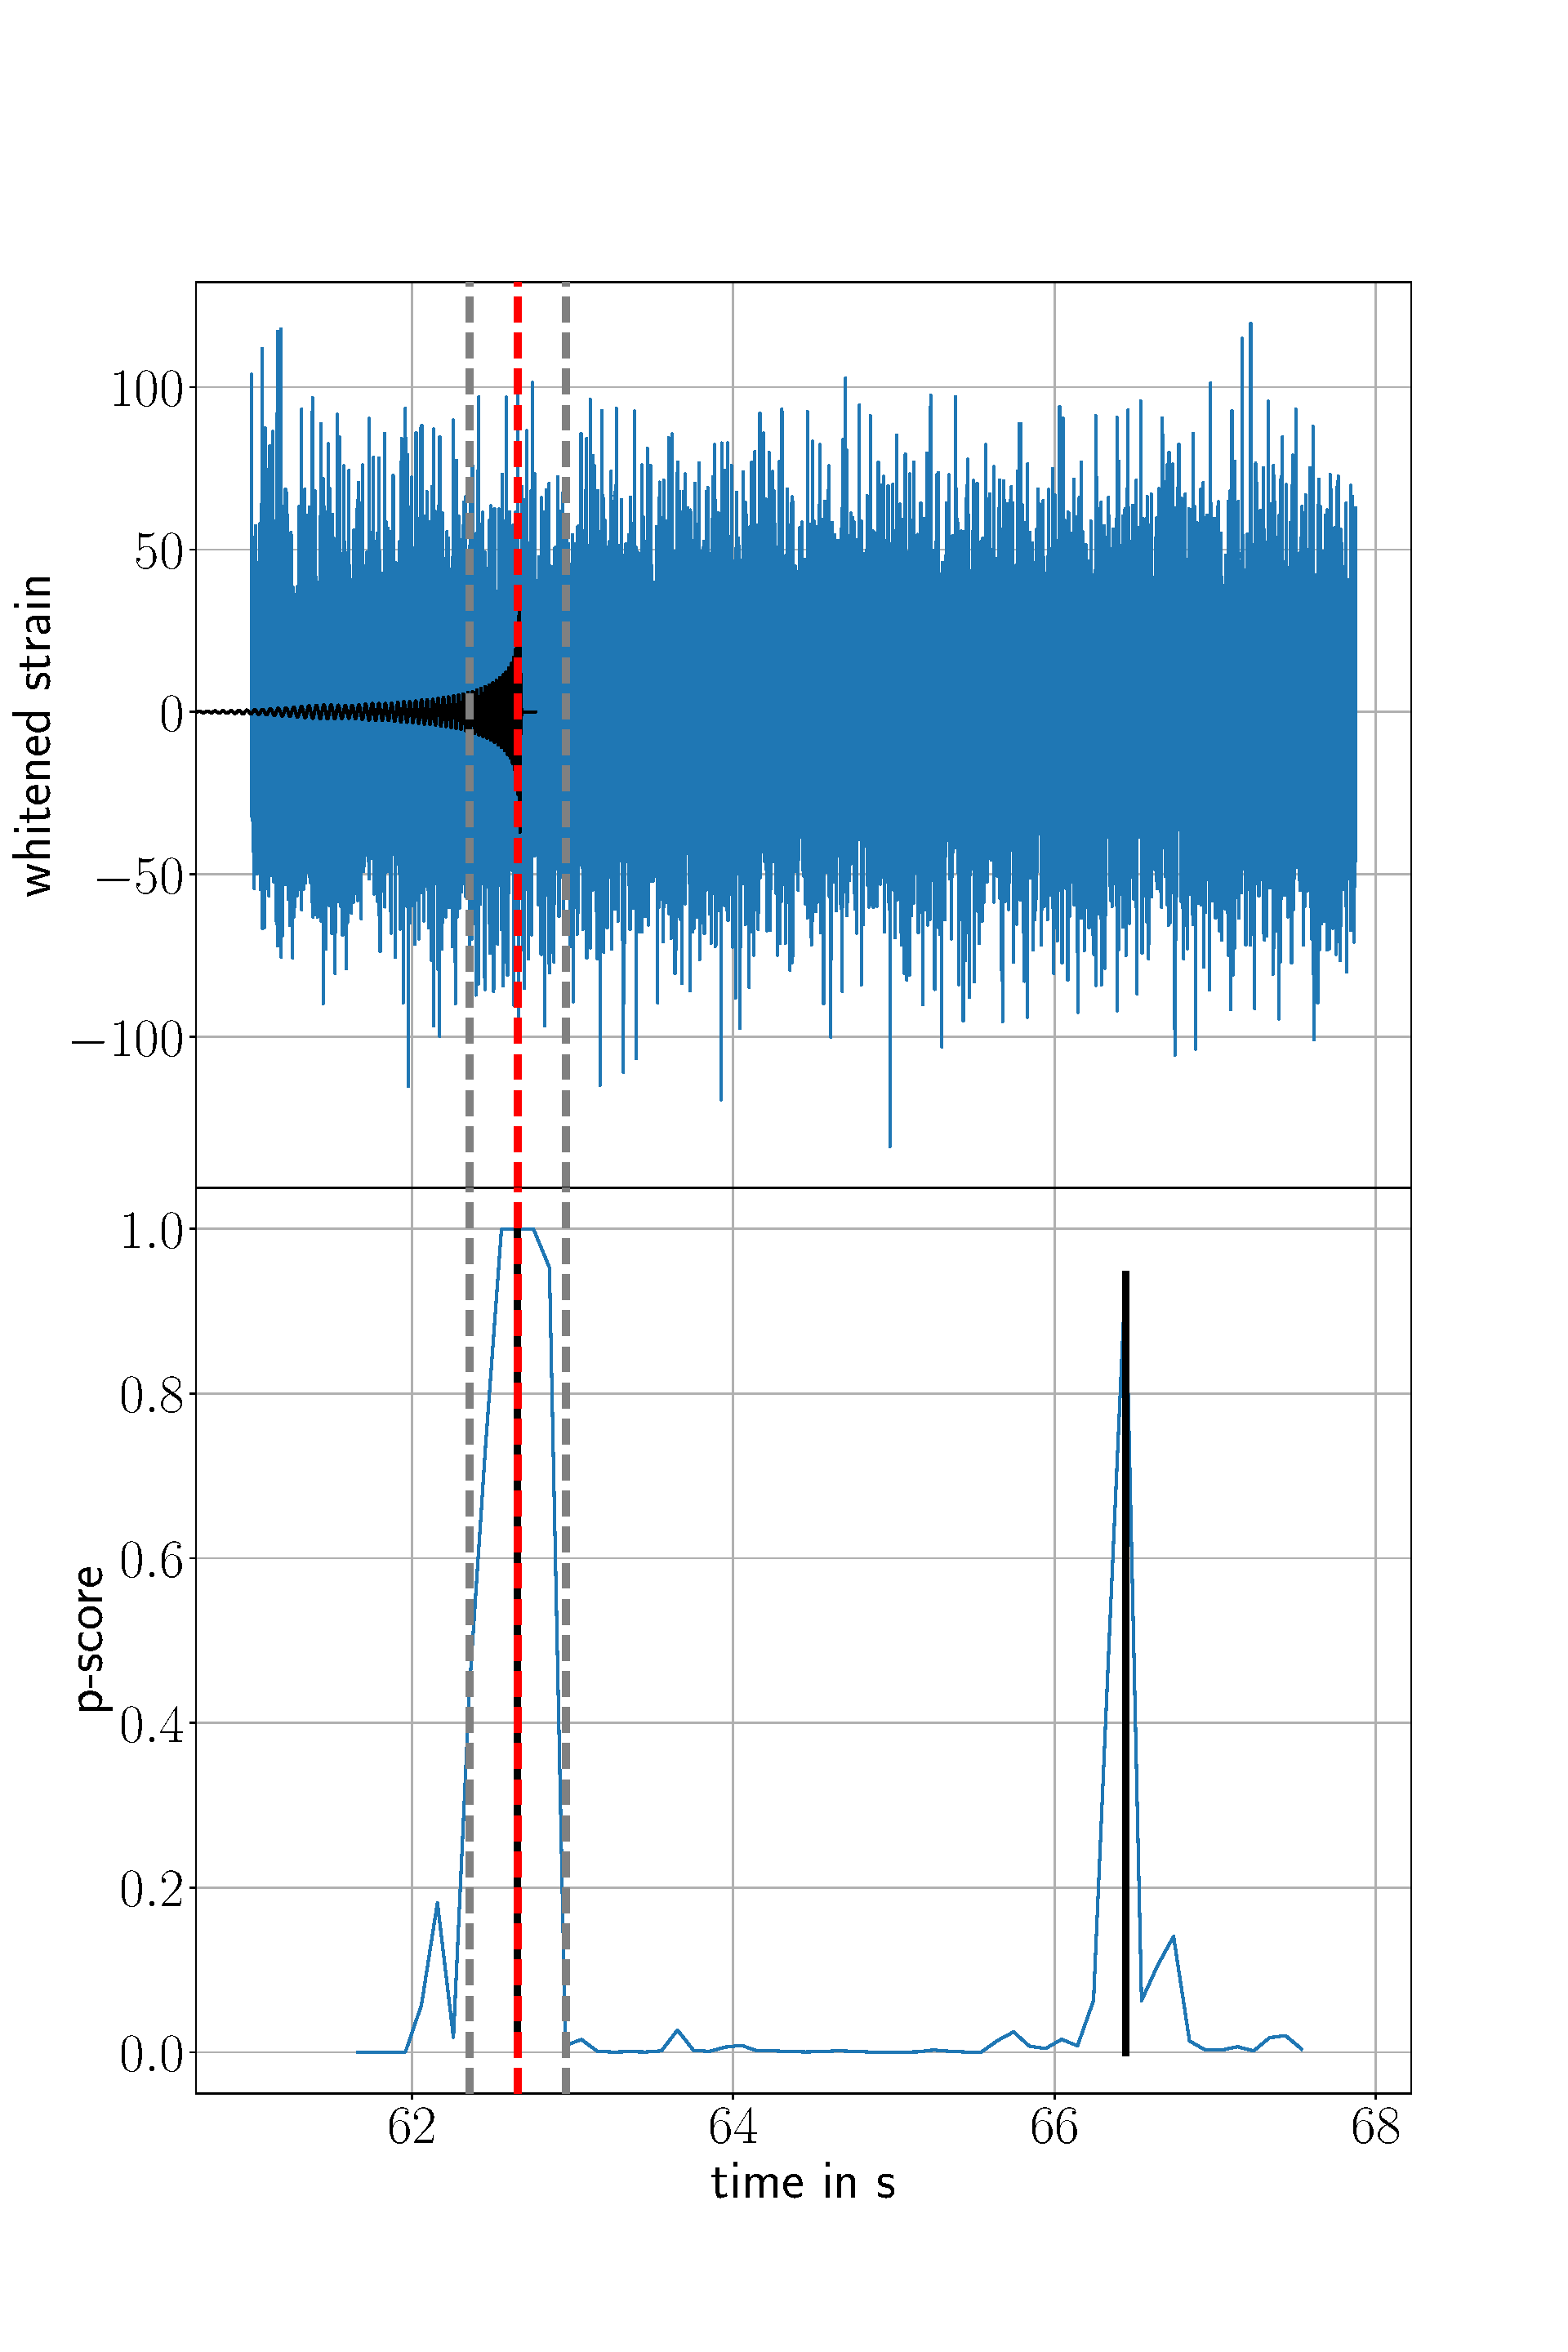
\includegraphics[width=0.7\textwidth]{chapters/training_strats/images/fixed_low_709.pdf}
    \caption[Sample output]{A sample output from the network on long duration data. The top panel shows the whitened input data. The injected signal is overlayed in black. The red vertical line signifies the time of the injection, i.e.\ the time that would ideally be returned by the search algorithm. The vertical grey lines mark the interval within which a returned event is classified as a true positive. The bottom panel shows the output of the network corresponding to the input. The vertical red and grey lines, again, show the true injection time and the allowed interval for true positives respectively. The black vertical lines mark the events returned by the search. Their height is the p-score attributed to the event. While the first event is a true positive, the second event is a false-positive originating from noise.}
    \label{fig:input_output}
\end{figure}

\subsection{Training strategies}\label{sec:methods:training_strategies}
The two initial publications by George et al.\ \cite{George:2016hay} and Gabbard et al.\ \cite{Gabbard:2017lja} disagree on the usefulness of curriculum learning. Whereas George et al.\ find a noticeable improvement by using curriculum learning, Gabbard et al.\ find no difference in the final performance of the network.

We aim to determine the impact curriculum learning has on the final performance and speed of convergence of these networks. By doing so we optimize the sensitivity of the networks tested here and hope that our findings generalize also to state-of-the-art machine learning search algorithms \cite{Krastev:2019koe, Schafer:2020kor, Gabbard:2019rde, Wei:2020ztw}.

Our study contains 10 curriculum learning and 5 fixed interval training strategies. An overview can be found in \autoref{tab:studies}. The minimum \acrshort{snr} allowed in any of these strategies is $\geq 5$. We choose \acrshort{snr} $5$ as a lower bound as this is roughly the lowest single detector \acrshort{snr} at which signals seen in multiple detectors can be confidently distinguished from noise \cite{LIGOScientific:2020ibl,Nitz:2021uxj}.

We test 5 different conditions for the optimal \acrshort{snr} contained in the training data for both types of strategies. For curriculum strategies, these conditions prescribe when the \acrshort{snr} of the training data is lowered. For fixed interval strategies the conditions are the interval from which the \acrshort{snr} for each sample is drawn.

Curriculum strategies use either the validation loss, the validation accuracy, or the number of epochs since the last step as conditions. For validation loss and validation accuracy we choose either a threshold or wait until the values stabilize and do not improve anymore. The latter are labeled by a prefix ''plateau'' throughout this paper. We choose a threshold of $0.95$ for the validation accuracy and $0.2$ for the validation loss. These values are arbitrary but proved to work well. When using the plateau conditions we lower the training range when the validation loss or validation accuracy, respectively, do not improve by more than $0.01\%$ for $6$ consecutive epochs. Finally, we also test lowering the training \acrshort{snr} irrespective of any of the metrics, by waiting 5 epochs between steps. We choose to wait $5$ epochs to allow the network enough time at each signal strength while ensuring we reach the minimum \acrshort{snr}. No extensive studies testing different values were made.

We test two different approaches to lowering the training \acrshort{snr}. All curriculum strategies start with \acrshort{snr}s which are uniformly drawn from the interval $\left[90, 100\right]$. Strategies that are given the postfix ''relative'' lower the bounds of this interval by $10\%$ at each step. The ranges are not lowered further when the lower bound of the interval reaches \acrshort{snr} $5$. Strategies without the postfix ''relative'' lower the bounds of the interval by a fixed value of $5$ at each step. This procedure is also continued down to a minimum bound of \acrshort{snr} $5$.

For fixed interval training strategies we test training on a single \acrshort{snr} as well as a fixed size interval of \acrshort{snr}s. We choose to train on fixed single \acrshort{snr}s $8$, $15$ and $30$ to cover the low, mid and high \acrshort{snr}s respectively. Training on a single \acrshort{snr} allows us to test how well the network generalizes to lower and higher \acrshort{snr}s than it has seen during training. By drawing the \acrshort{snr} from an interval we aim to reduce the dependence on a specific signal strength. We choose two strategies that draw \acrshort{snr}s from a fixed range. One covers only the lowest range used by any of the non-relative curriculum strategies, i.e.\ it draws the signal \acrshort{snr}s from the interval $\text{\acrshort{snr}}\in\left[5,15\right]$. The other draws the \acrshort{snr}s from the entire range of \acrshort{snr}s seen by the curriculum strategies, $\text{\acrshort{snr}}\in\left[5,100\right]$.

\begin{table}
\caption[Training strategy overview]{An overview of the different training strategies tested in this work. The ''Curriculum'' type strategies lower the \acrshort{snr} of the training samples whenever the condition in the last column is fulfilled. All of them start with  $\mathrm{SNR}\in\left[90, 100\right]$. Curriculum strategies with the postfix ''relative'' in their name lower the boundaries of the interval by $10\%$ at each step, until the lower limit falls below \acrshort{snr} 5. The other curriculum strategies lower the bounds by a fixed value of $5$, until the lower limit reaches \acrshort{snr} 5. A metric fulfills the plateau condition when it has not improved by more than $0.01\%$ for $6$ consecutive epochs. The ''Fixed interval'' type strategies use a single \acrshort{snr} range for the entire training. Their interval is given in the last column. }
\label{tab:studies}
\begin{tabularx}{\textwidth}{l|l|X}
    \hline\hline
    \multicolumn{1}{l}{Type} & \multicolumn{1}{l}{Name} & \multicolumn{1}{l}{Condition} \\
    \hline
    \multirow{12}{*}{Curriculum} & accuracy & \multirow{2}{*}{\parbox[t]{\linewidth}{when validation accuracy $\geq 0.95$}}\\
    \cline{2-2}
    & accuracy relative & \\
    \cline{2-3}
    & epochs & \multirow{2}{*}{every 5 epochs} \\
    \cline{2-2}
    & epochs relative & \\
    \cline{2-3}
    & loss & \multirow{2}{*}{\parbox[t]{\linewidth}{when validation loss $\leq 0.2$}} \\
    \cline{2-2}
    & loss relative & \\
    \cline{2-3}
    & plateau accuracy & \multirow{3}{*}{\parbox[t]{\linewidth}{6 epochs validation accuracy plateau}} \\
    \cline{2-2}
    & plateau accuracy & \\
    & relative & \\
    \cline{2-3}
    & plateau loss & \multirow{3}{*}{\parbox[t]{\linewidth}{6 epochs validation loss plateau}} \\
    \cline{2-2}
    & plateau loss & \\
    & relative & \\
    \hline
    \multirow{5}{*}{Fixed interval} & \acrshort{snr} 30 & $\mathrm{SNR}=30$ \\
 \cline{2-3}
    & \acrshort{snr} 15 & $\mathrm{SNR}=15$ \\
    \cline{2-3}
    & \acrshort{snr} 8 & $\mathrm{SNR}=8$ \\
     \cline{2-3}
    & low & $\mathrm{SNR}\in \left[5, 15\right]$ \\
     \cline{2-3}
    & full & $\mathrm{SNR}\in \left[5, 100\right]$ \\
    \hline\hline
\end{tabularx}
\end{table}

\subsection{Matched-filter baseline}\label{sec:methods:mf}
In order to assess how sensitive the trained networks are in relation to conventional searches, we perform a matched-filter analysis of the test set described in \autoref{sec:methods:general}. To do so, we utilize the PyCBC analysis toolkit \cite{pycbc-github}.

The template bank covers component masses from \SIrange{10}{50}{M_\odot} and is constructed to lose no more than $3\%$ of the \acrshort{snr} of any signal due to its discreteness. The templates are placed stochastically. In total, the bank contains $598$ templates.

The search is implemented by \verb|pycbc_inspiral|. We configured it to output a set of times where any template of the bank convolved with the data exceeds a matched-filter \acrshort{snr} of $5$. Unlike the optimal \acrshort{snr}, the matched-filter \acrshort{snr} is the match of a detector data segment with a template, and so it varies based on the noise realization, while the optimal \acrshort{snr} assumes a noise realization that is constant zero. Combining the times where the threshold is exceeded with the corresponding matched-filter \acrshort{snr} and by using this \acrshort{snr} as ranking statistic, we obtain a set of triggers. We then process these triggers as described in \autoref{sec:methods:network_performance} to find events and calculate \acrshort{far}s and sensitive distances.

The configuration files are included in the data release \cite{ml-training-strategies-github}.

\section{Results}\label{sec:train_strat_results}
\subsection{Sensitivities}\label{sec:results:sensitivities}
We are able to reproduce or in some cases even improve on the results given in \cite{Gabbard:2017lja}. The top panel of \autoref{fig:efficiency_example} shows the efficiency of one network as a function of the \acrshort{snr} at fixed \acrshort{fap}s calculated on the efficiency set. We compare our findings to theirs and find excellent agreement with the results shown in Figure 3 of \cite{Gabbard:2017lja}, which closely reproduced efficiencies of matched filtering. The efficiencies at \acrshort{fap}s down to $10^{-3}$ for most other training strategies also closely follow the findings of Gabbard et al. We are, therefore, able to robustly reproduce the findings of \cite{Gabbard:2017lja}.

\begin{figure}
    \centering
    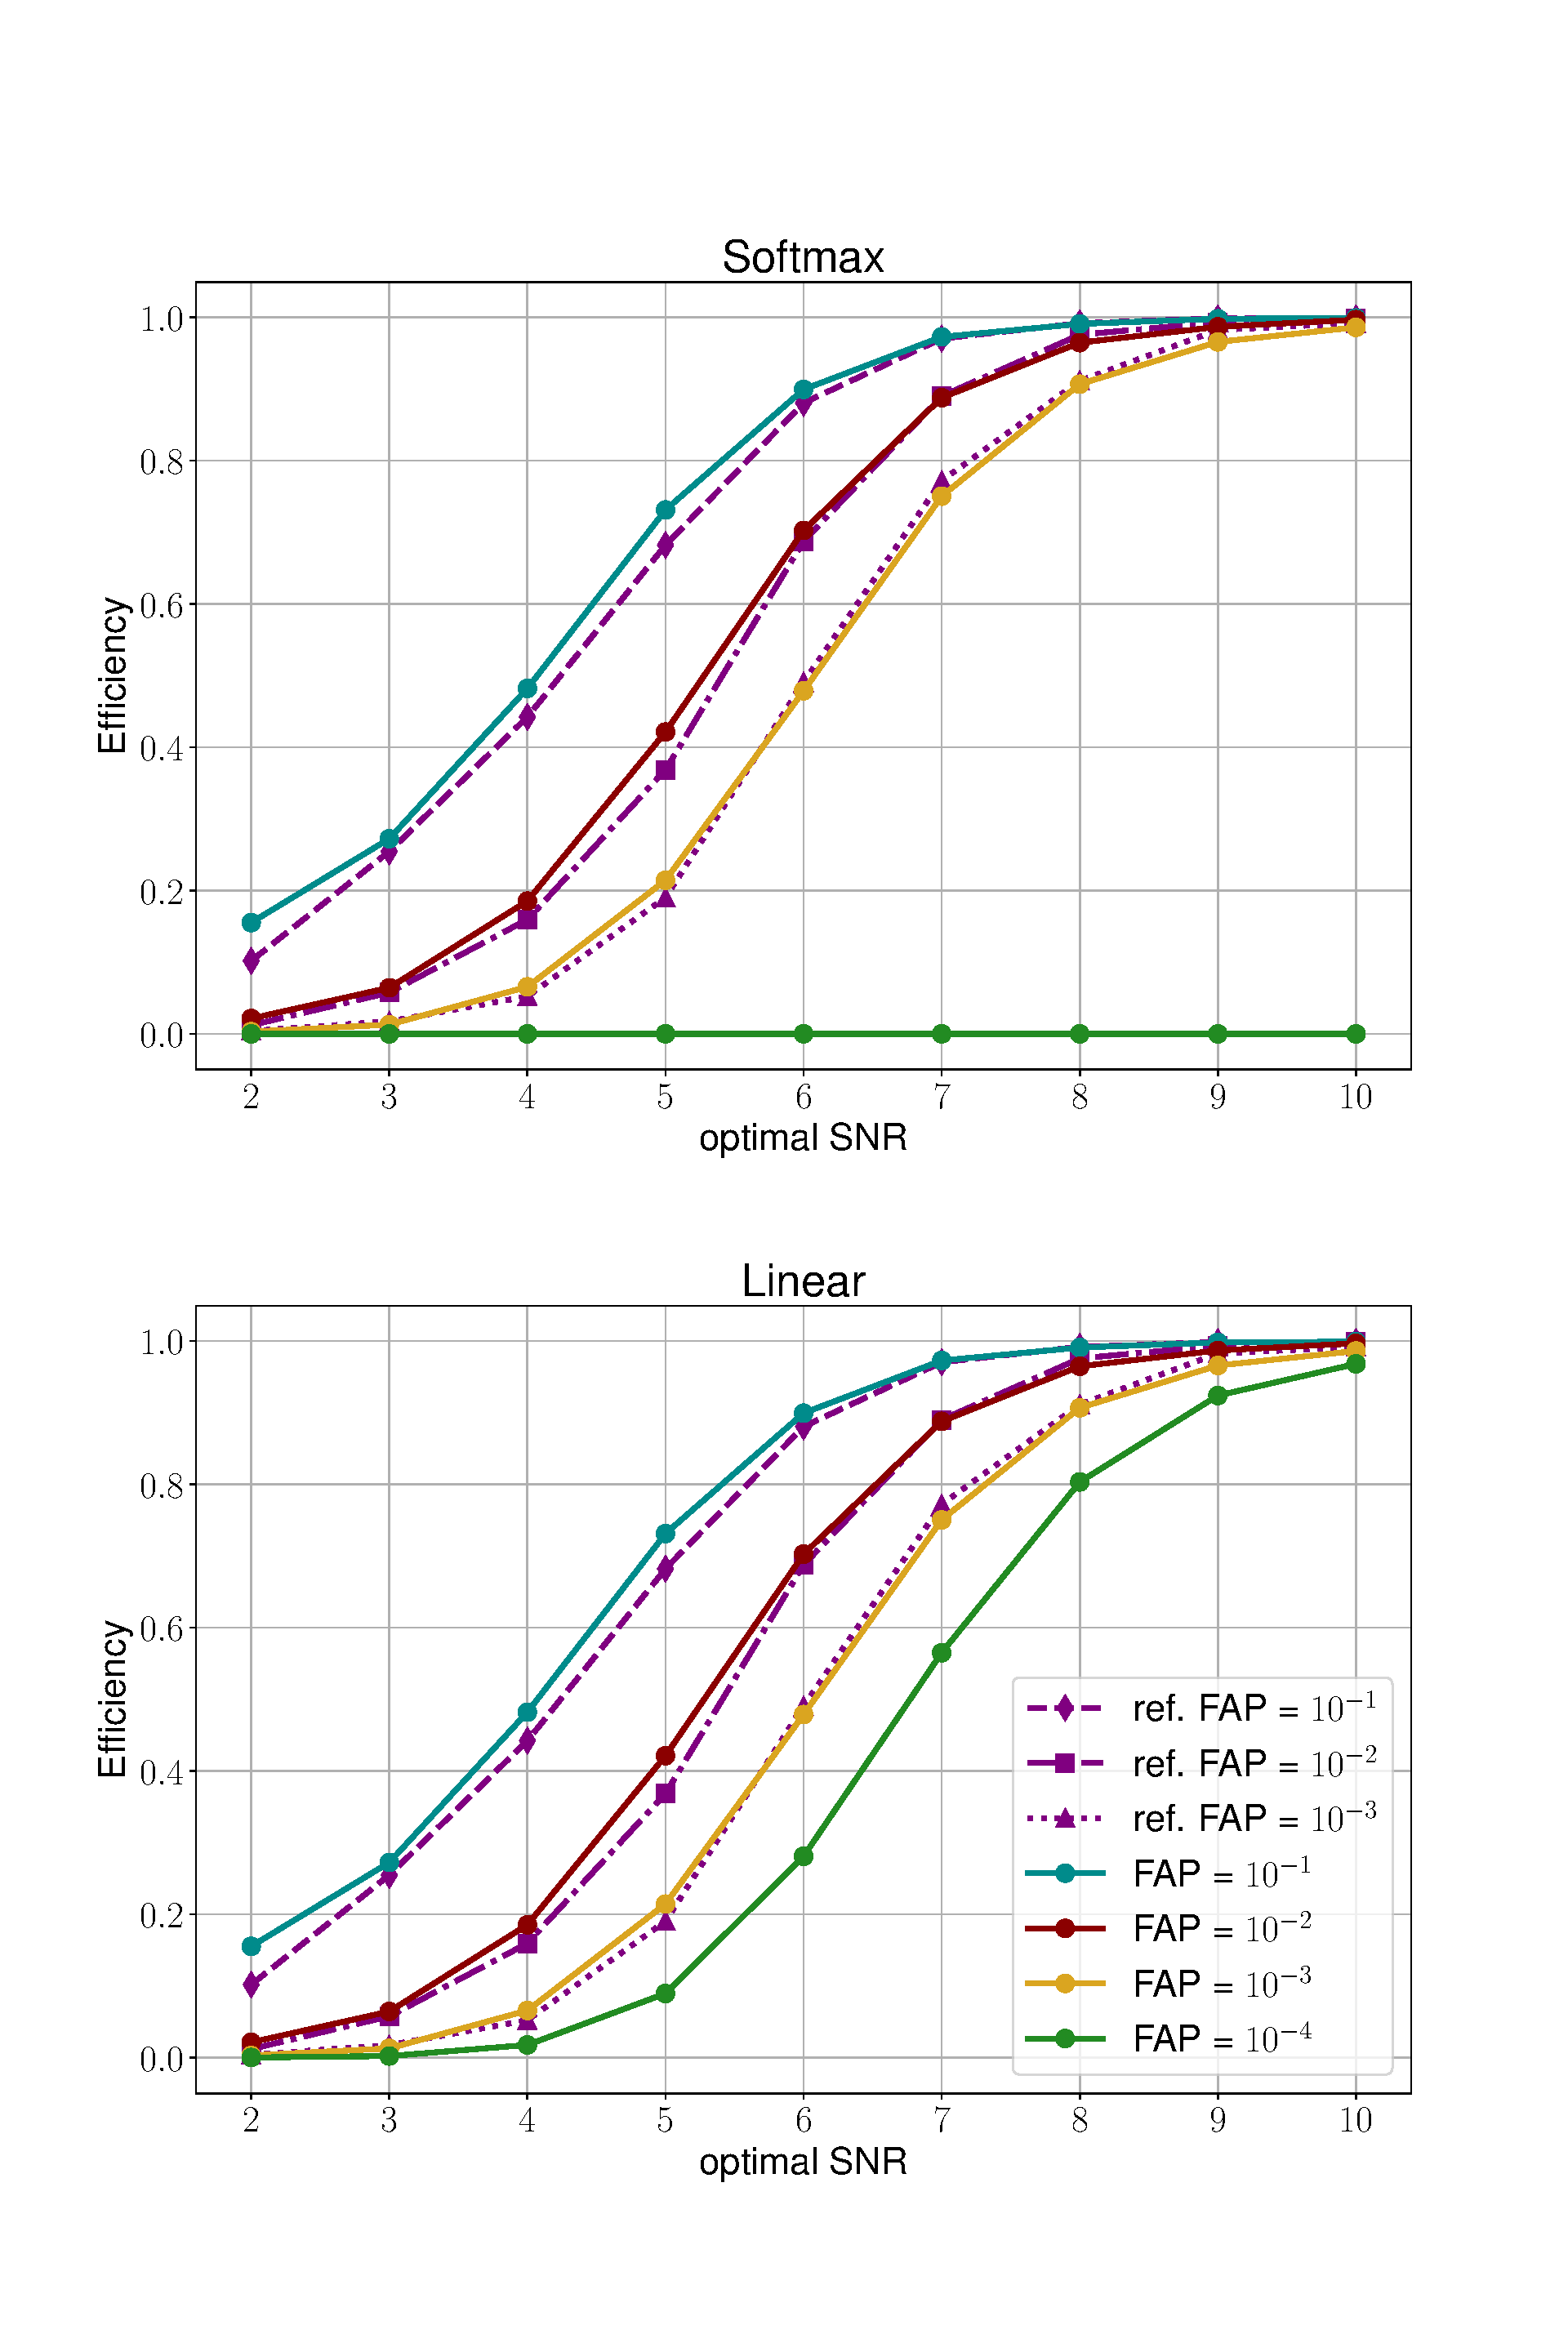
\includegraphics[width=0.7\textwidth]{chapters/training_strats/images/fixed_low_743_186.pdf}
    \caption[Network efficiency at different signal-to-noise ratios]{The efficiency as a function of optimal \acrshort{snr} at different \acrshort{fap}s. The network was trained on \acrshort{snr}s drawn from the fixed interval $\left[5,15\right]$. We used epoch $186$ of the network with the lowest efficiency at that epoch to produce this figure. The top panel shows the efficiency when the last layer uses a Softmax activation, the bottom panel shows the same network with the \acrshort{usr} modification. We determine the threshold on the network output using a set of $400\,000$ pure noise samples. Any of the $10\,000$ signals at each \acrshort{snr} exceeding this threshold are counted as detected. We compare our findings to Figure 3 of the reference \cite{Gabbard:2017lja} which closely reproduces efficiencies of matched filtering.}
    \label{fig:efficiency_example}
\end{figure}

In \autoref{fig:efficiency_evolution_fixed_low} we show the evolution of the efficiency of the $50$ networks trained on the fixed interval $\text{\acrshort{snr}}\in\left[5,15\right]$ as the number of training epochs is increased at a \acrshort{fap} of $10^{-4}$. Each panel of the plot shows the efficiency for a chosen \acrshort{snr} which allows us to observe how well the networks perform during different stages of the training at different signal strengths. This is especially interesting for curriculum strategies, where the \acrshort{snr} in the training set is adjusted as the network trains. The grey lines show the evolution of the efficiency for the different network initializations. The black, dashed line is the average of the grey lines. We highlight the evolution of a single network in dark grey. The red, dashed, vertical line signifies the epoch of maximum efficiency over all $50$ networks and $200$ epochs. 
\begin{figure*}
    \centering
    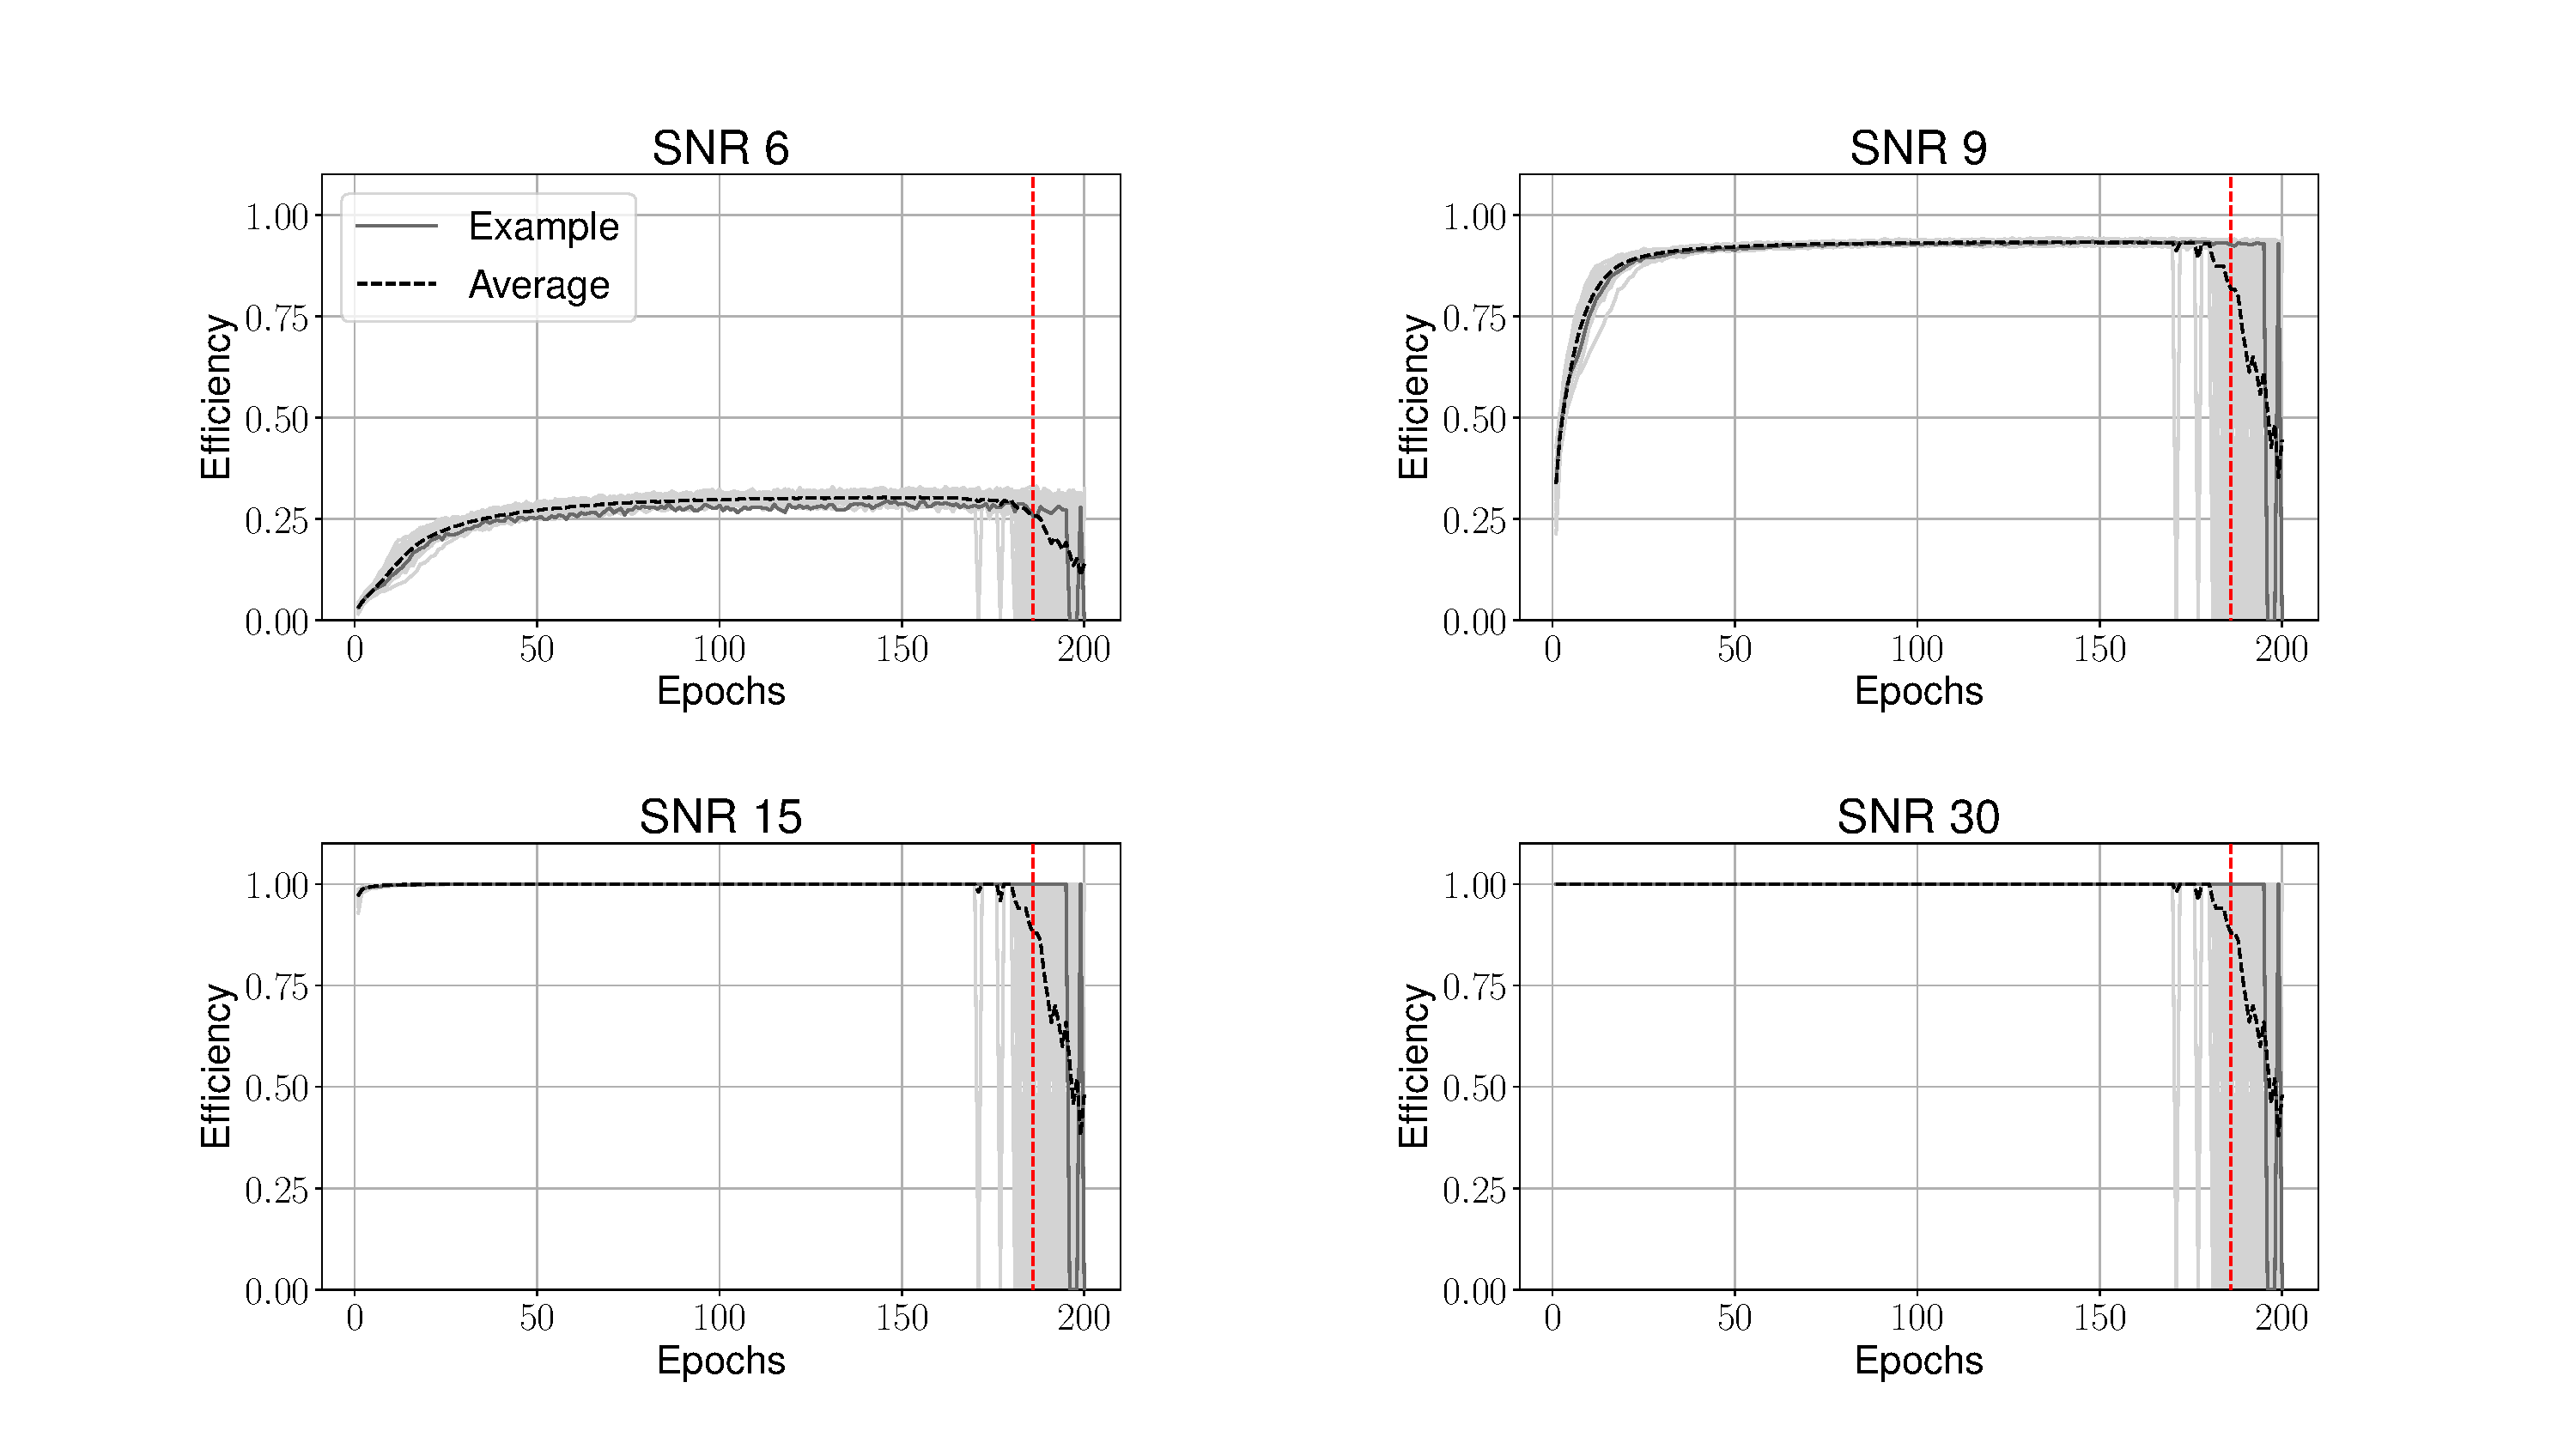
\includegraphics[width=\textwidth]{chapters/training_strats/images/fixed_low_soft.pdf}
    \caption[Network efficiency evolution fixed low strategy with Softmax]{The evolution of the efficiency as a function of the epochs at different optimal \acrshort{snr}s. Training used the fixed \acrshort{snr} interval $\left[5,15\right]$. The individual evolutions of all $50$ runs are included as grey curves that form overlapping grey bands when plotted together. The dashed black line is the average of those. In dark grey we highlight the evolution of the efficiency for a single network. At the epoch marked by the red, dashed, vertical line we select the network with the highest, lowest and closest to average efficiency for further testing. The curves are computed at a \acrshort{fap} of $10^{-4}$.}
    \label{fig:efficiency_evolution_fixed_low}
\end{figure*}

All networks in \autoref{fig:efficiency_evolution_fixed_low} converge to similar efficiencies during the first $\sim 100$ epochs. However, as training continues sudden drops to zero efficiency occur which become more frequent at later epochs. As a result the average efficiency drops continuously after some time. All networks show this behavior and thus the influence of an unlucky initialization can be ruled out. Furthermore, the drops are observed at all \acrshort{snr}s simultaneously and, therefore, do not depend on the signal strength.

The same effect can be seen in the top panel of \autoref{fig:efficiency_example}. For $\text{\acrshort{fap}s}\geq 10^{-3}$ the curves behave as expected. As one lowers the \acrshort{fap} the efficiency at any given \acrshort{snr} is expected to drop. Visually this manifests in a shift of the efficiency curves toward higher \acrshort{snr}s. Ideally, this behavior would be true for any \acrshort{fap}. However, at a \acrshort{fap} of $10^{-4}$ the efficiency collapses and becomes a constant $0$.

The drops to zero efficiency are caused by noise samples which are attributed a p-score of 1. Since the Softmax activation on the last layer restricts outputs to the interval $\left[0, 1\right]$, no signal samples can achieve a p-score larger than the threshold and thus they cannot be distinguished from noise.

Many of the noise samples attributed a p-score of 1 are caused by numerical rounding errors in the Softmax activation 
\begin{equation}\label{eq:softmax}
    {\text{Softmax}\left(\bm{x}\right)}_i=\frac{\exp\left(x_i\right)}{\sum_{j=0}^N \exp\left(x_j\right)} ~,
\end{equation}
where $\bm{x} = \left(x_0, x_1, \hdots, x_N\right)$ is the vector of outputs of the previous layer in the network, and $N+1$ is the number of neurons in the layer.

The networks operate with single precision (32-bit) floating point numbers. Therefore, small changes in the values of $\bm{x}$ may cause a roundoff error due to the rapid change in scale of the exponential functions. When this occurs, the fraction may evaluate to $1$ even when mathematically \eqref{eq:softmax} may never be $1$.

We removed the final activation of the pre-trained network in an attempt to avoid the rounding errors. To do so, we recast \eqref{eq:softmax} for $N=1$ into
\begin{equation}\label{eq:recast_softmax}
    \frac{\exp\left(x_0\right)}{\exp\left(x_0\right)+\exp\left(x_1\right)}=\frac{1}{1+\exp\left(x_1-x_0\right)},
\end{equation}
and impose thresholds for the efficiency calculation on the difference $x_0-x_1$ directly rather than ${\text{Softmax}\left(\bm{x}\right)}_0$. Since \eqref{eq:recast_softmax} is bijective, there exists a direct relation between thresholds in $x_0-x_1$ and the thresholds on $\text{Softmax}\left(\bm{x}\right)_0$. We use $x_0-x_1$ rather than $x_1-x_0$ as our ranking statistic since $x_0-x_1>\hat{x}_0-\hat{x}_1\Leftrightarrow {\text{Softmax}\left(\bm{x}\right)}_0>{\text{Softmax}\left(\bm{\hat{x}}\right)}_0$. We call this modification unbounded Softmax replacement.

The resulting efficiency is depicted in the bottom panel of \autoref{fig:efficiency_example}. \autoref{fig:efficiency_evolution_fixed_low_lin} shows the efficiency evolution at different optimal \acrshort{snr}s. We find that the drops to zero efficiency vanish when we apply \acrshort{usr}. This is the case for all training strategies we explored and more examples are shown in the appendix (see \autoref{fig:efficiency_evolution_acc_rel_soft} to \autoref{fig:efficiency_evolution_fixed_30_lin}).

\begin{figure*}
    \centering
    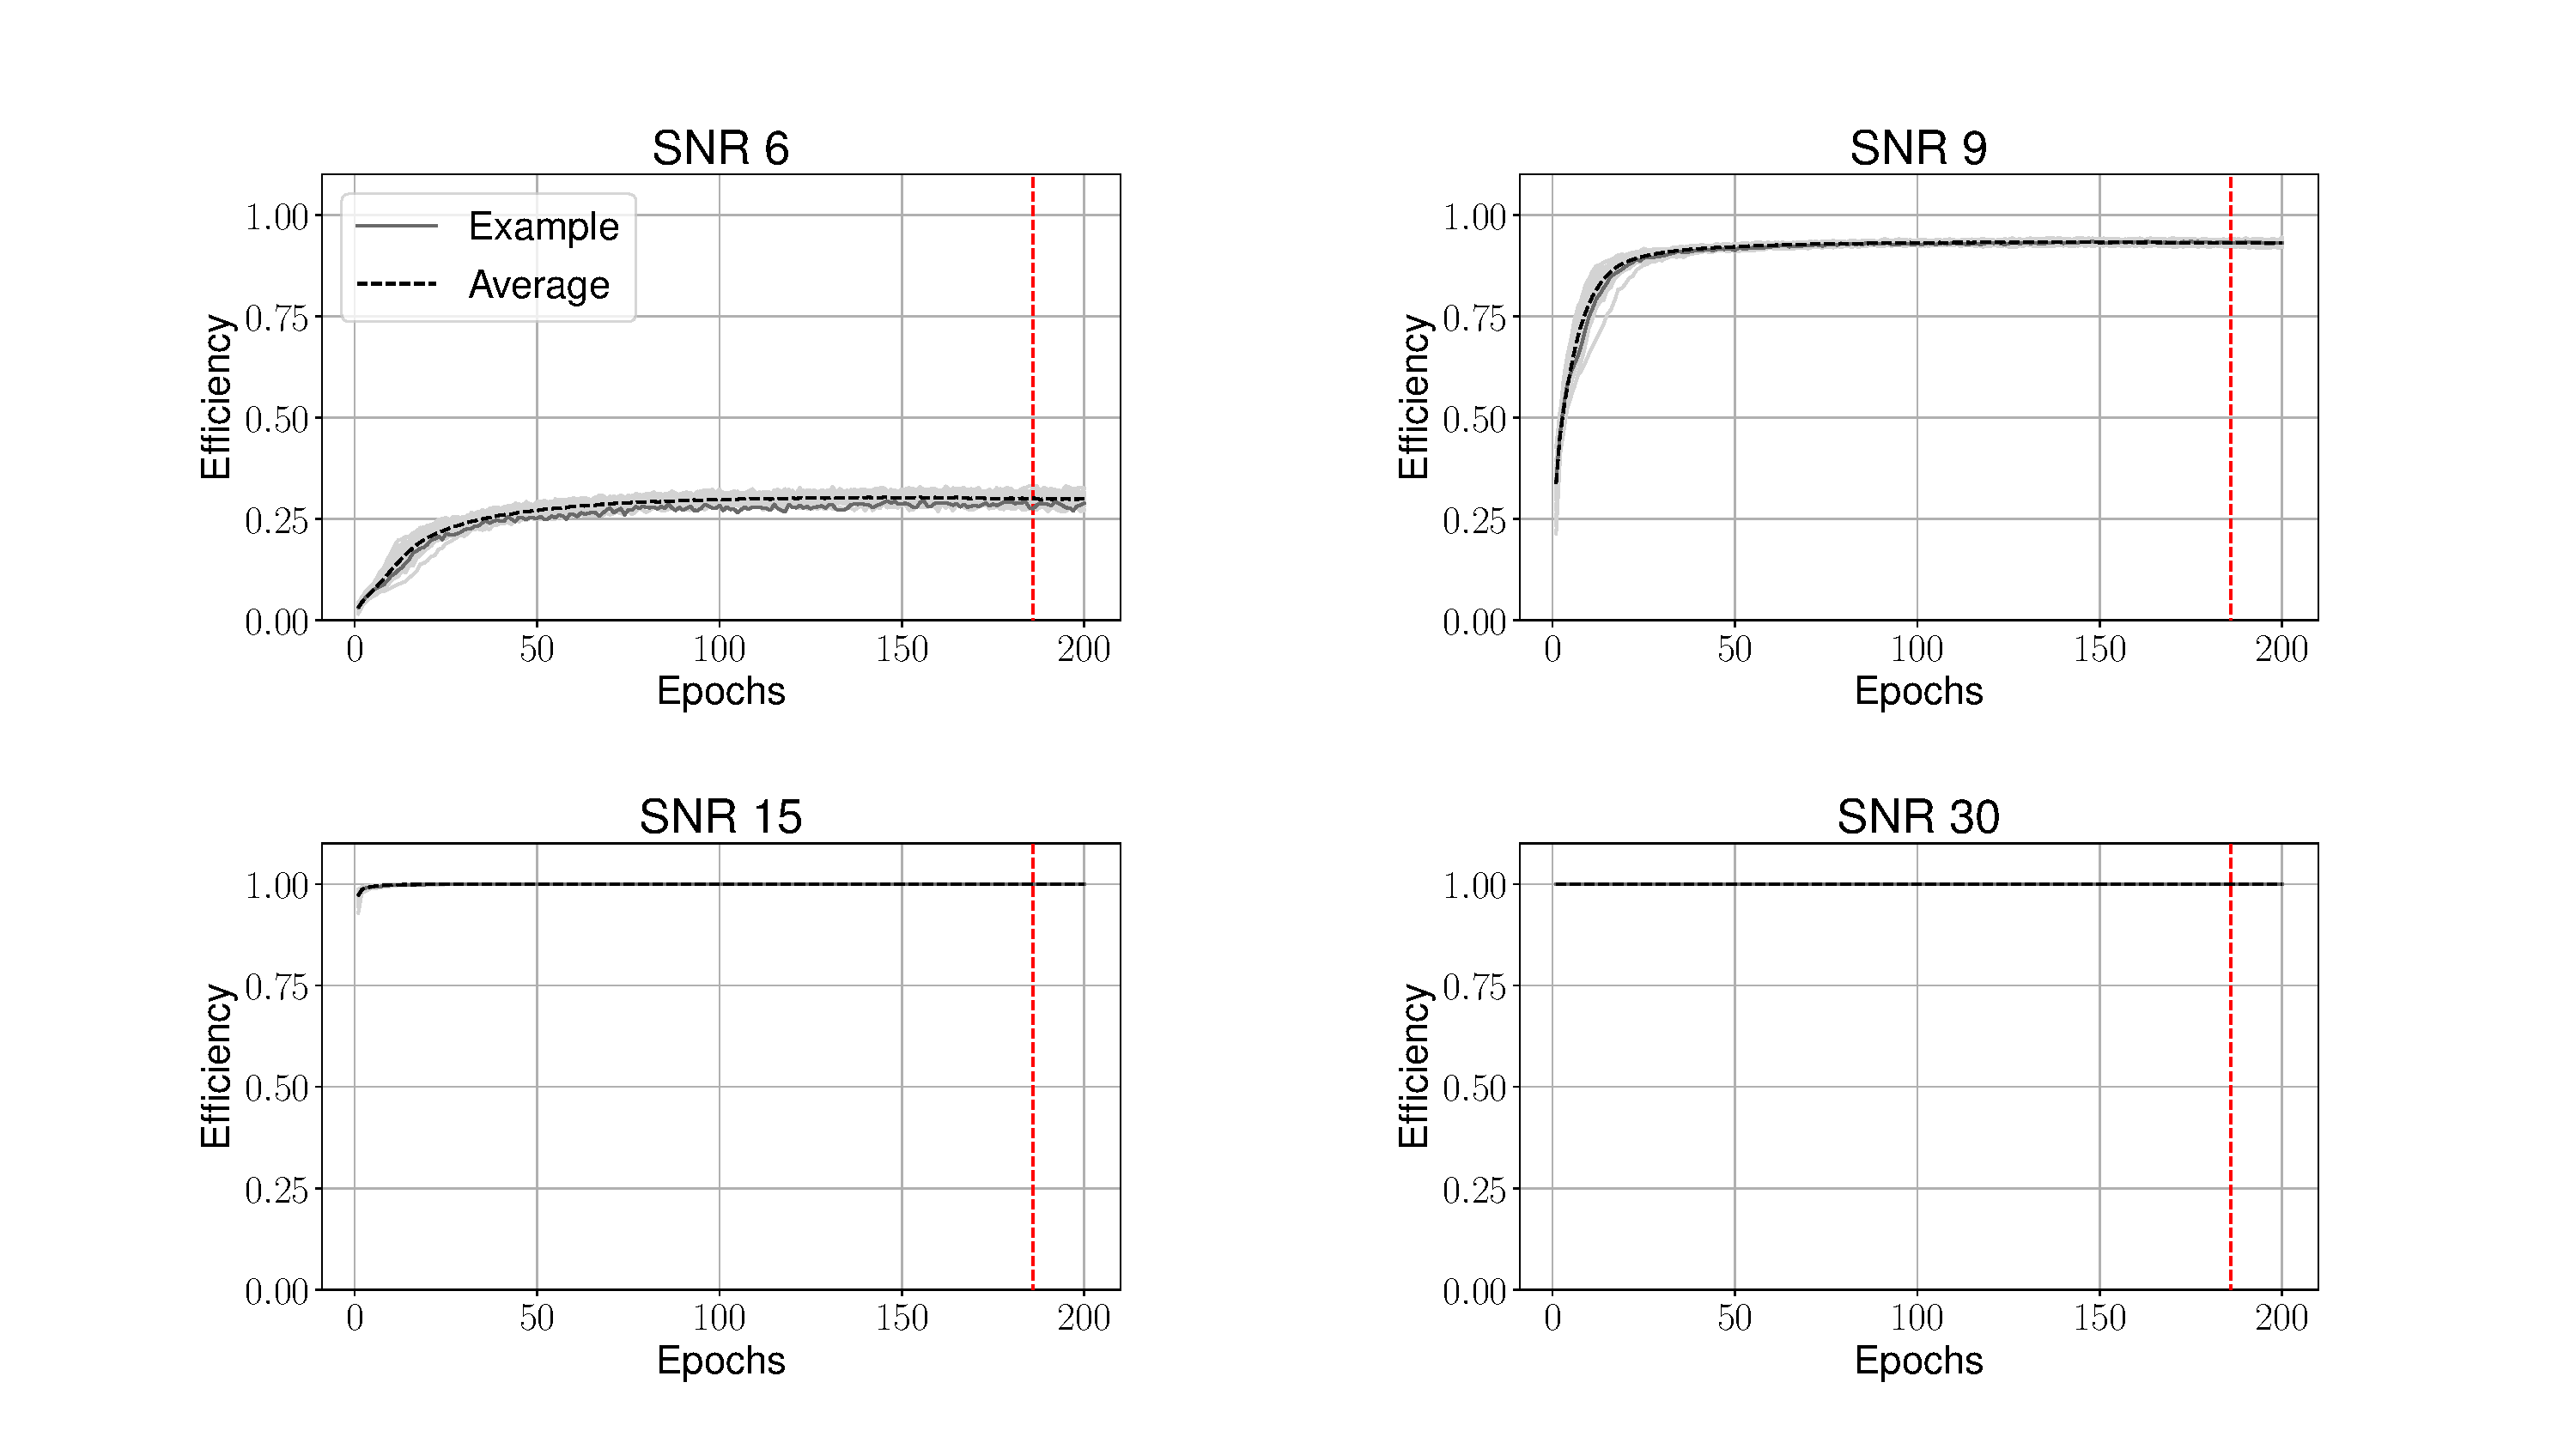
\includegraphics[width=\textwidth]{chapters/training_strats/images/fixed_low_lin.pdf}
    \caption[Network efficiency evolution fixed low strategy with unbounded Softmax replacement]{The evolution of the efficiency as a function of the epochs at different optimal \acrshort{snr}s. Training used the fixed \acrshort{snr} interval $\left[5,15\right]$. The individual evolutions of all $50$ runs are included as grey curves that form an overlapping grey band when plotted together. The dashed black line is the average of those. In dark grey we highlight the evolution of the efficiency for a single network. At the epoch marked by the red, dashed, vertical line we select the network with the highest, lowest and closest to average efficiency for further testing. The curves are computed at a \acrshort{fap} of $10^{-4}$. This figure shows the same networks as \autoref{fig:efficiency_evolution_fixed_low} after applying \acrshort{usr}. This prevents the efficiency to drop to 0.}
    \label{fig:efficiency_evolution_fixed_low_lin}
\end{figure*}

One could also try to resolve the rounding issue by using double precision (64-bit) floating point numbers instead of single precision when applying the Softmax layer. We have tested a numerically safe implementation of the Softmax and found that its first output is rounded up to one even for quadruple (128-bit) precision when the difference $x_0-x_1>45$. This is a relatively low value that indeed occurs for some noise realizations in our experiments. Although using higher precision for the Softmax layer increases the range of values it can operate on, the \acrshort{usr} still solves roundoff issues more robustly.

The efficiency is a metric that is easy to calculate and physically more relevant than the accuracy of the network. However, it does not deal with samples where waveforms are misaligned in the data or take into account longer stretches of time. It is, therefore, only an approximation to the true statistic we want to calculate: the sensitive volume.

To assess if the efficiency is a good approximation to this statistic, we calculate the sensitive volume of three chosen networks for every training strategy as described in \autoref{sec:methods:network_performance}. The networks are chosen from the $50$ different initializations based on their efficiency at a selected epoch. We pick the networks with the highest, lowest and closest to average efficiency and denote them with ''High'', ''Low'' and ''Mean'', respectively, from here on out. If the efficiency at a fixed \acrshort{fap} is a good indicator of the networks sensitivity we expect the sensitive volume to scale with the efficiency.

\autoref{fig:sensitivity_fixed_low} shows the sensitive distance as a function of the \acrshort{far} computed for the three networks trained on the fixed, low \acrshort{snr} interval. It compares the networks with (dashed) and without (continuous) the final Softmax activation and shows an equivalent matched-filter search in purple as reference. We find that the network is sensitive to sources up to a distance of \SI{2150}{\mega\parsec} with $1$ false alarm per month.

\begin{figure}
    \centering
    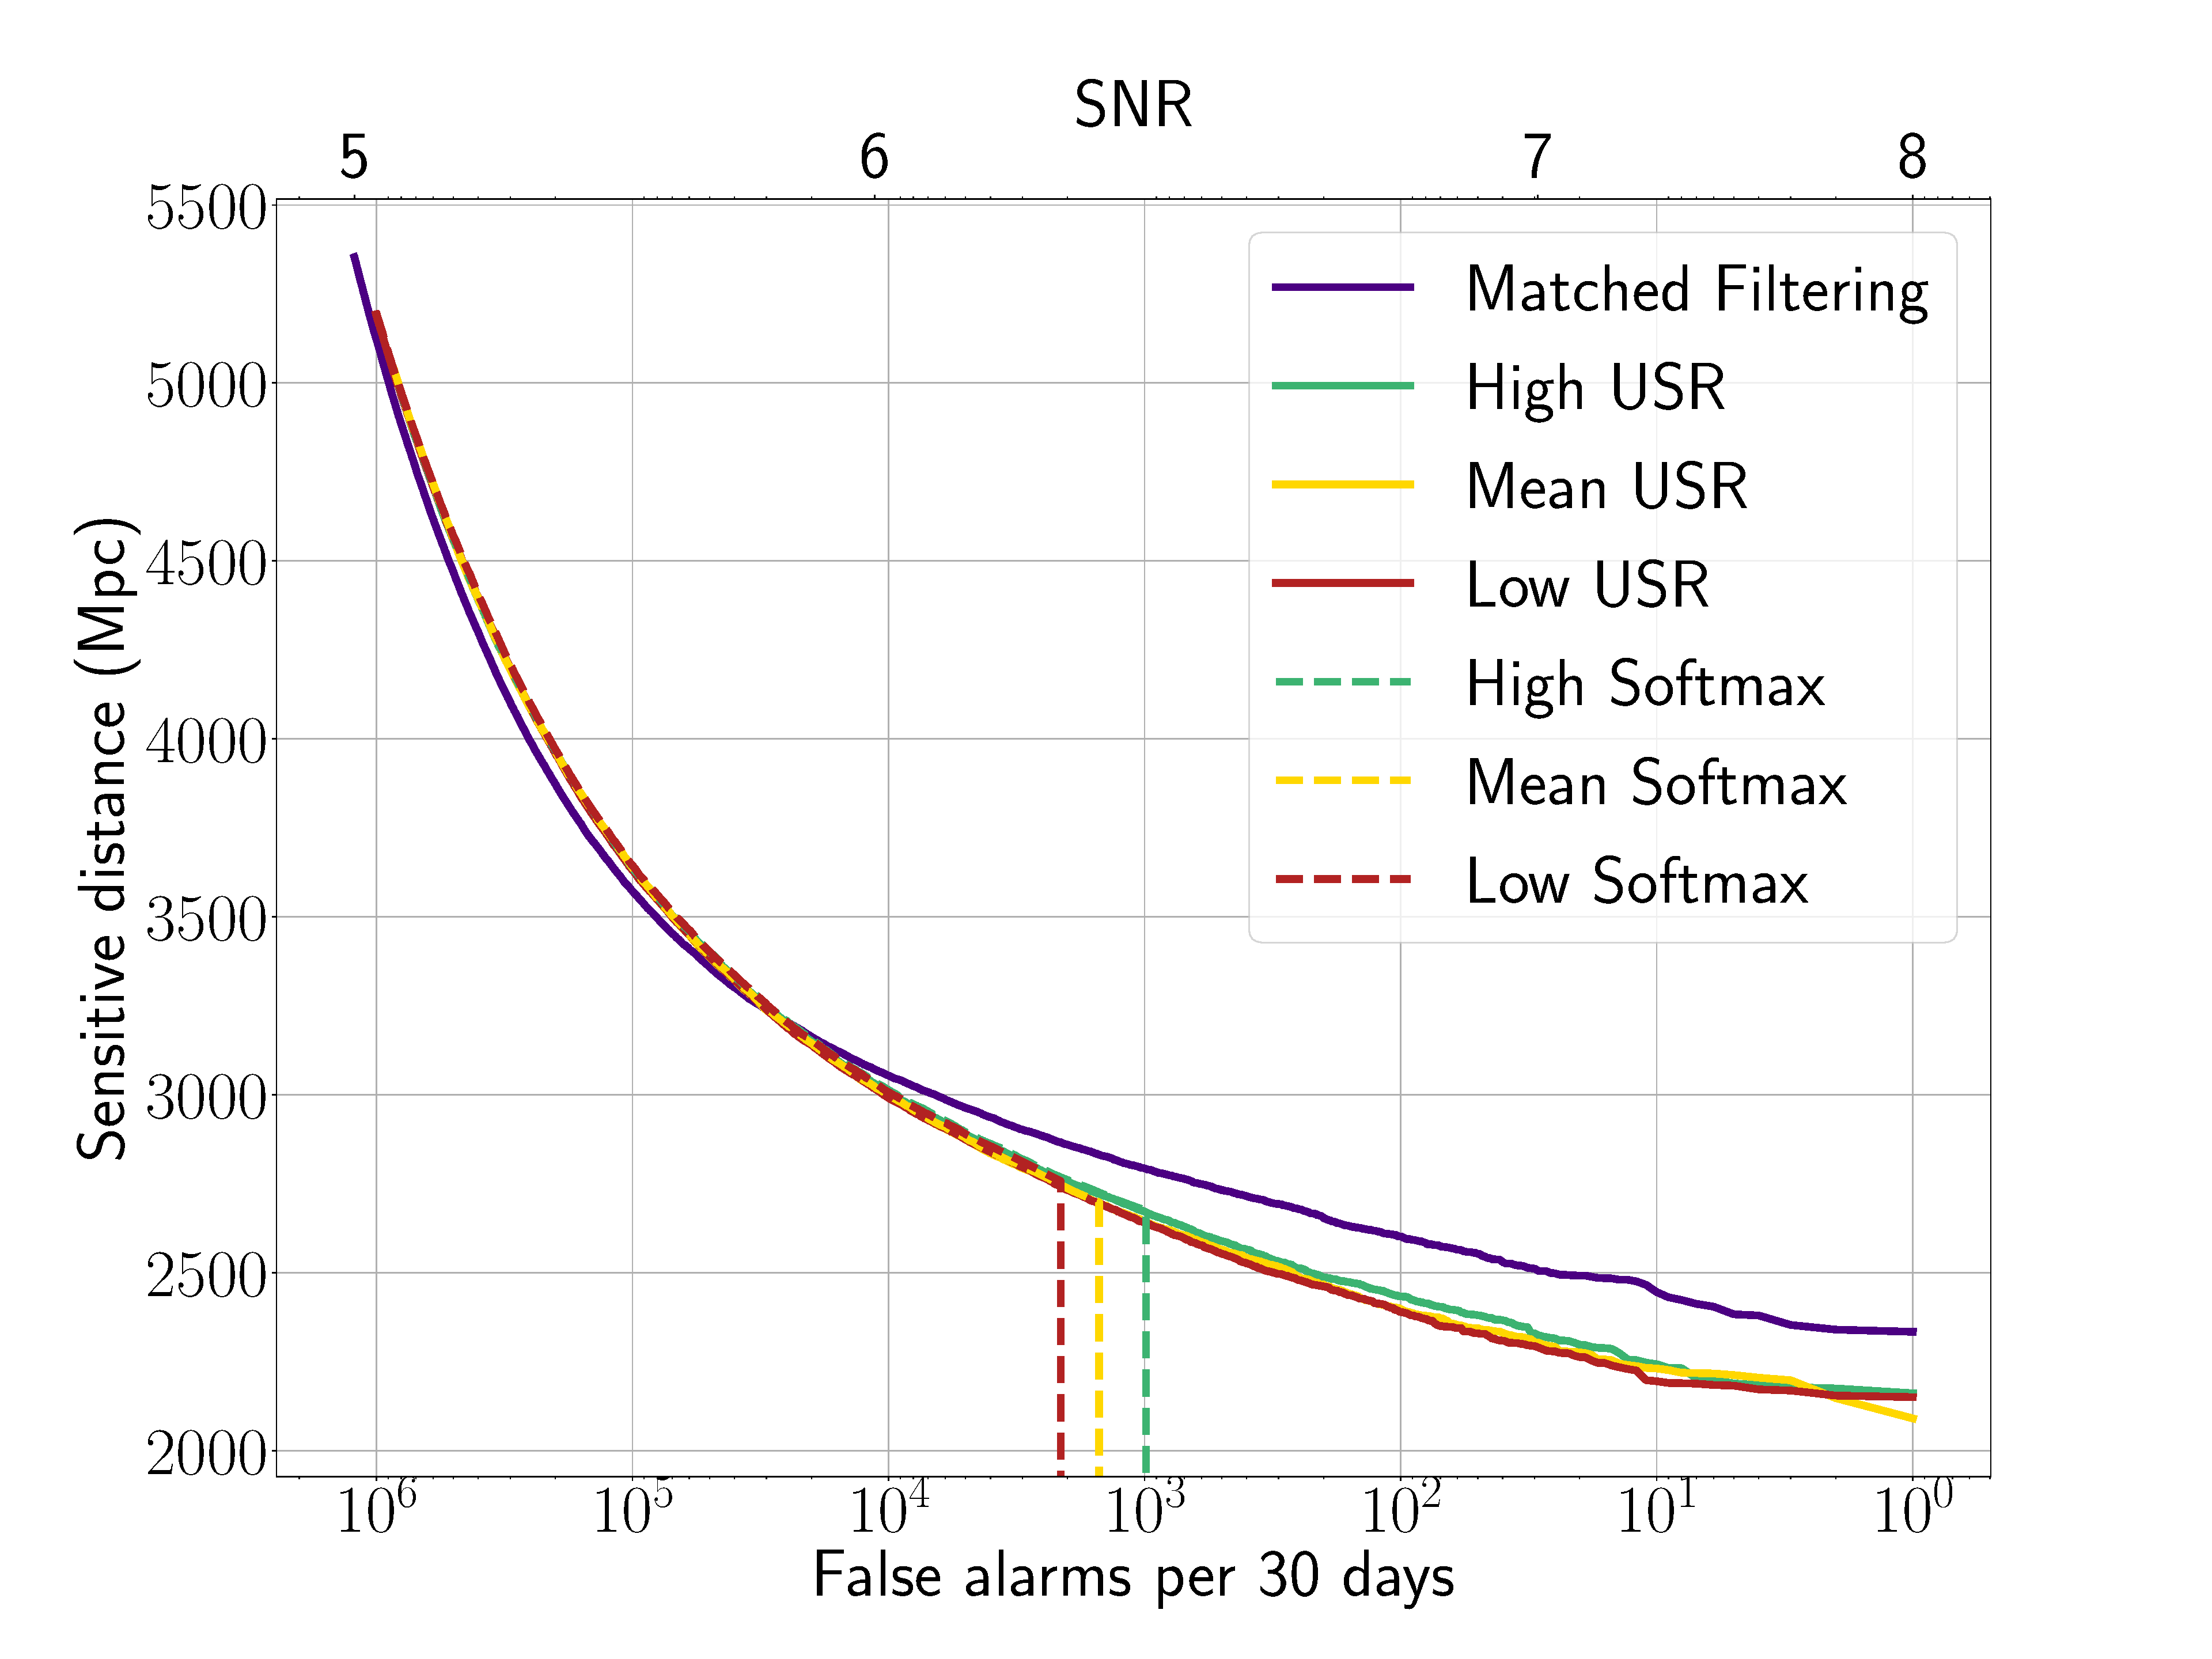
\includegraphics[width=0.7\textwidth]{chapters/training_strats/images/fixed_low_sens.pdf}
    \caption[Sensitive distance plot]{The sensitive distance as a function of the \acrshort{far} (bottom horizontal axis) for different search algorithms. We compare differently initialized networks trained on data containing signals with \acrshort{snr} $\in\left[5,15\right]$ to an equivalent matched-filter search. The dashed lines show the original networks, the filled lines show the corresponding network when \acrshort{usr} is applied. The labels ''High'' (green), ''Mean'' (yellow) and ''Low'' (red) correspond to the networks with the highest, closest to average and lowest efficiency at epoch $186$, respectively. In purple we show the equivalent matched-filter search that operates with a template bank containing $598$ templates. The top horizontal axis shows the \acrshort{snr} threshold for the matched-filter search corresponding to the \acrshort{far} on the bottom axis.}
    \label{fig:sensitivity_fixed_low}
\end{figure}

The sensitive radii of all converged deep learning searches lie within $3.4\%$ of each other for \acrshort{far}s where all of them are non-zero. However, the sensitivity of the networks with the final Softmax activation drops to zero for \acrshort{far}s $\leq\mathcal{O}(10^3)$ per month. This drop is caused by $\mathcal{O}(10^3)$ false alarms with a p-score of 1. This saturation of the final activation can be alleviated by applying the \acrshort{usr} modification and using the new output as a ranking statistic.

All tested networks have also been re-evaluated using higher precision floating point data types for the final activation function evaluation (example shown in Fig. \ref{fig:precision_sensitivities}). This resulted in the networks remaining sensitive at \acrshort{far}s down to $3$ per month. However, applying the \acrshort{usr} modification allowed us to test the network down to a \acrshort{far} of $1$ per month. Additionally, casting to a higher precision considerably increases computation time in the network due to hardware optimizations of GPUs for single precision floating point operations. In our view, the effectiveness of the \acrshort{usr} outweights the benefits of using higher precision, hence we only report results obtained with the \acrshort{usr} modification.

\begin{figure}
    \centering
    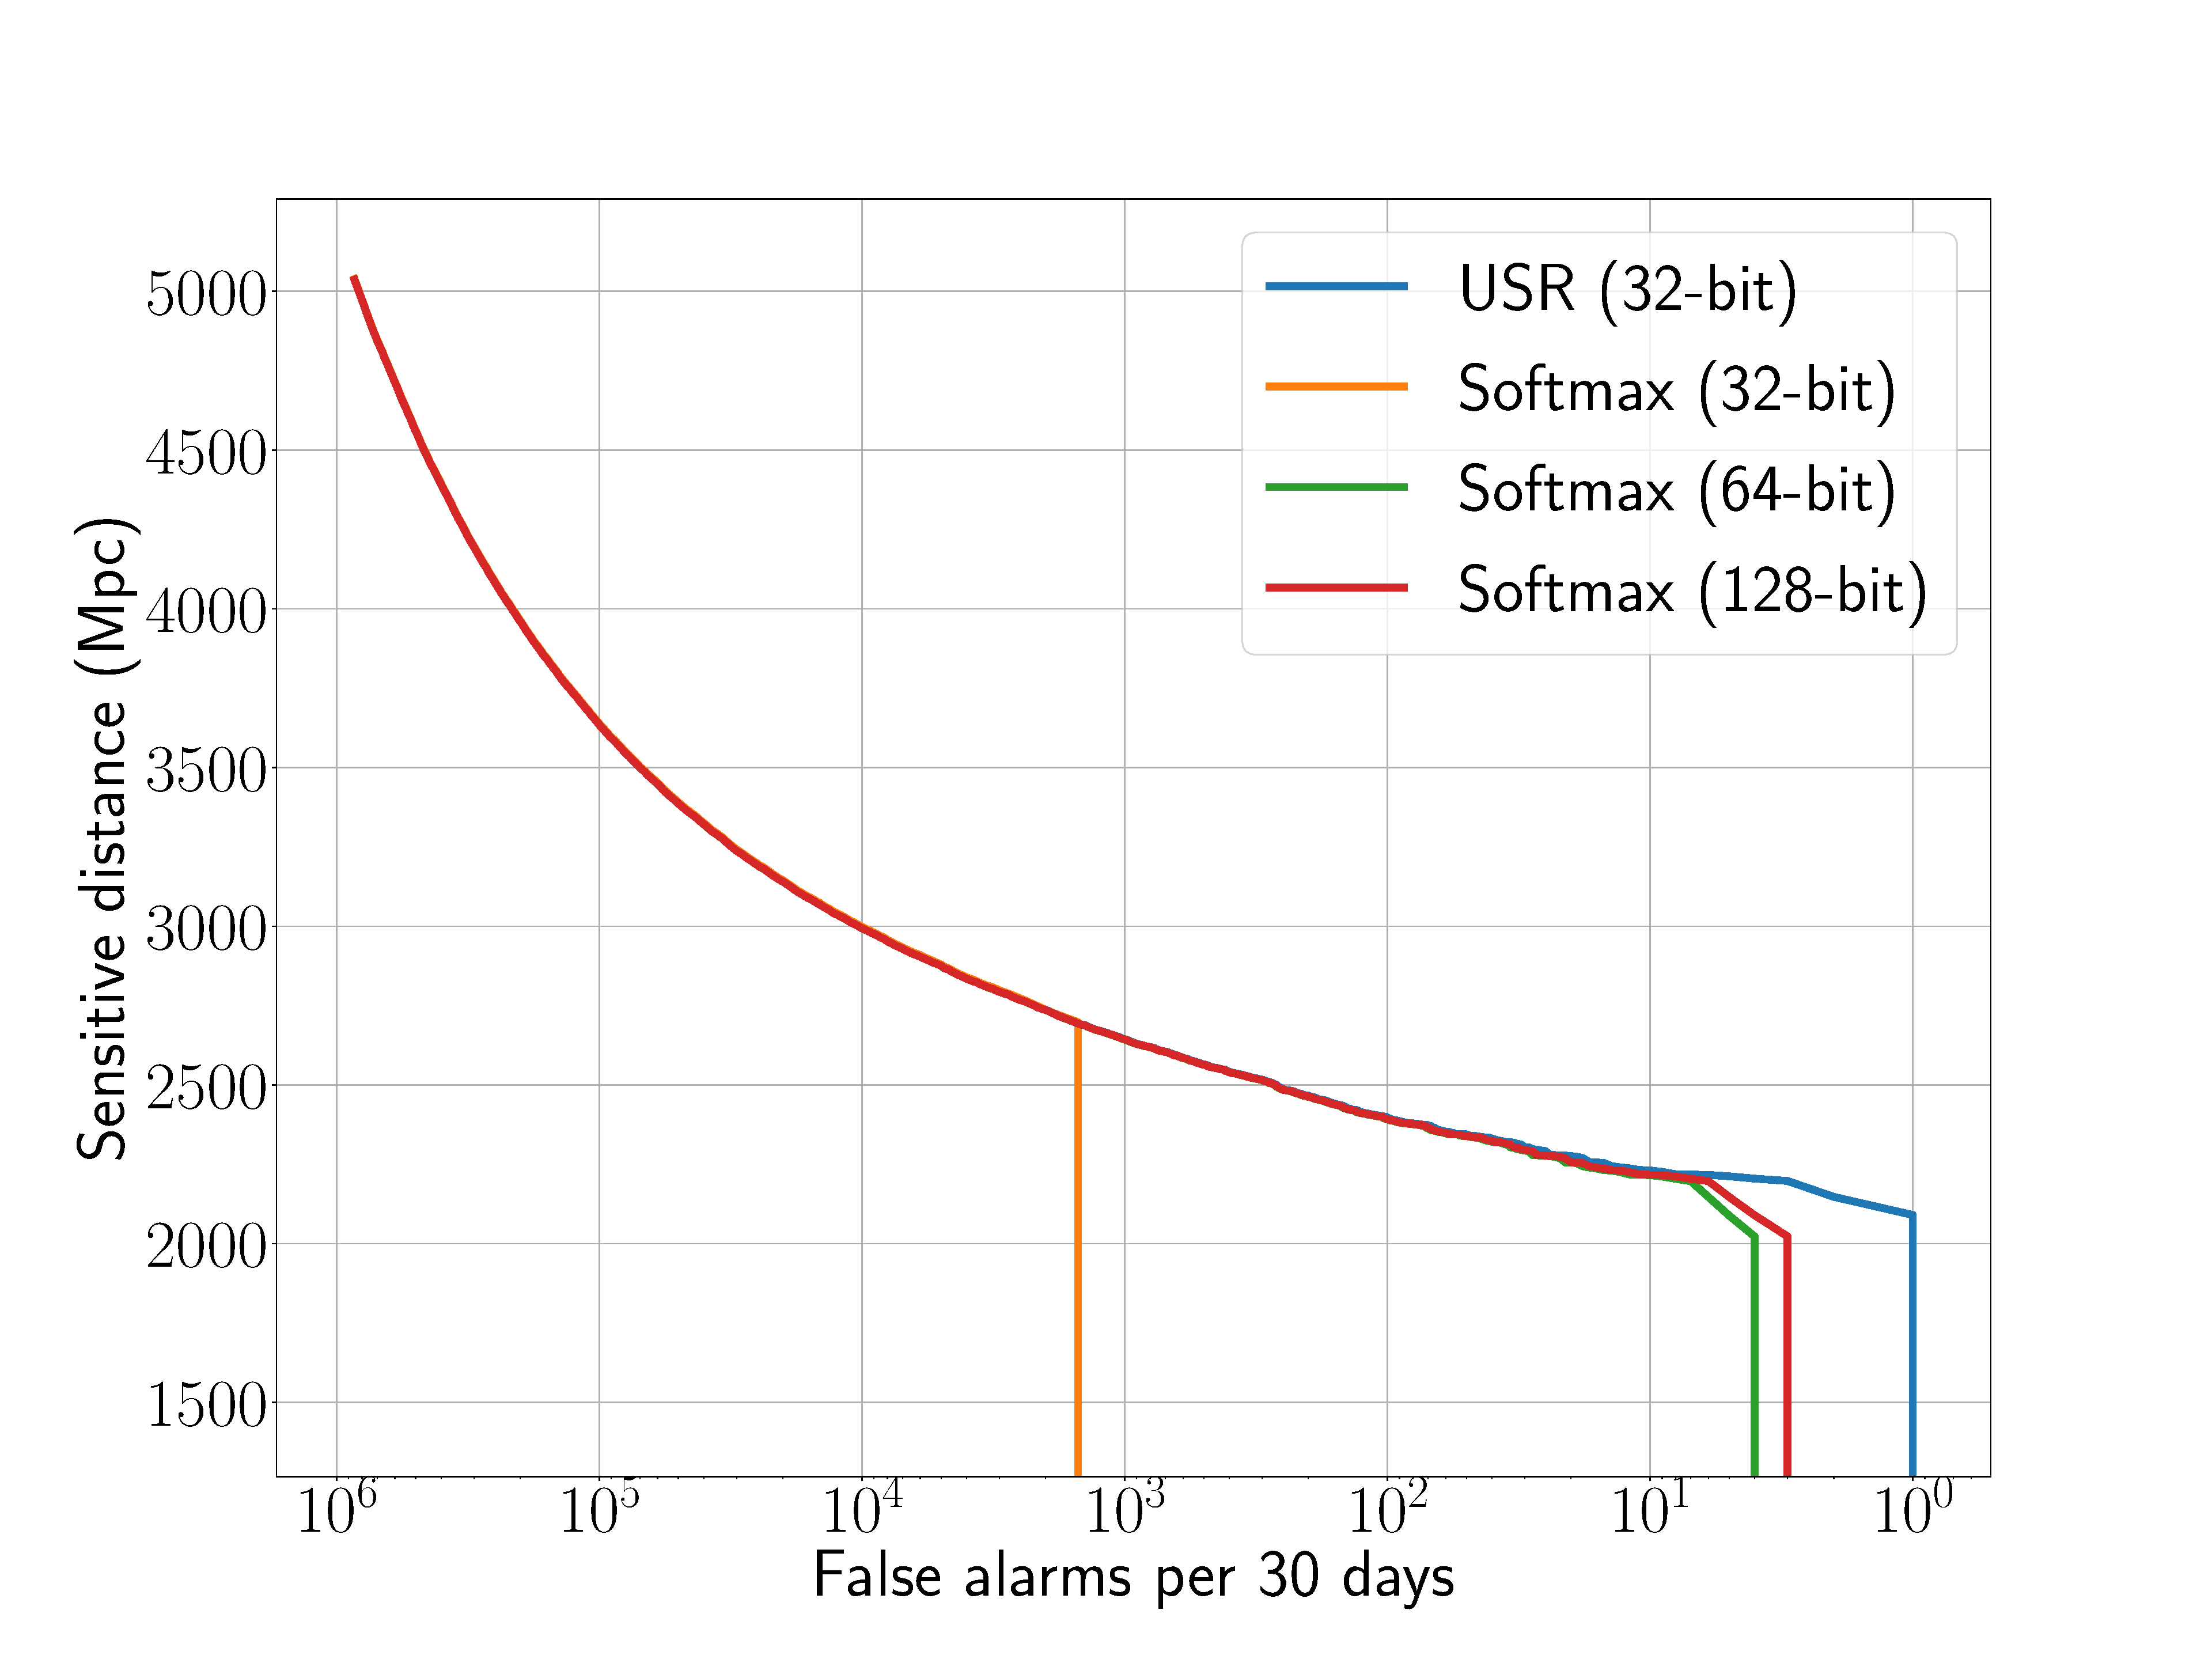
\includegraphics[width=0.7\textwidth]{chapters/training_strats/images/precision_712.pdf}
    \caption[Sensitive distance of different floating point precisions]{Sensitivity of the "mean" run of the "fixed low" strategy using the Softmax layer of various floating point precisions as well as the USR. A similar behavior of USR performing at least as well as the Softmax with all precisions was observed in all 45 evaluated runs.}
    \label{fig:precision_sensitivities}
\end{figure}

We had expected to find networks with higher efficiencies to be more sensitive, even within different initializations of the same training strategy. As such in \autoref{fig:sensitivity_fixed_low} we expected to find the sensitivity curve labeled ''High'' to be above the one labeled ''Mean'' above the one labeled ''Low''. While this is true in the example shown in \autoref{fig:sensitivity_fixed_low} in some regions, for other training strategies the order is arbitrary. All initializations converge to basically the same sensitivity. Sensitivity plots for all training strategies are provided in the data release \cite{ml-training-strategies-github}.

The machine learning algorithms are compared to an equivalent matched-filter search, shown in purple in \autoref{fig:sensitivity_fixed_low}. All searches perform equally well for \acrshort{far}s $\geq 10^5$ per month. For smaller \acrshort{far}s the matched-filter search is sensitive to sources which are up to \SI{200}{\mega\parsec} farther away. The deep learning search retains at least $91.5\%$ of the sensitivity compared to the matched-filter search at all \acrshort{far}s.

This result shows that with minimal modification to the architecture the original network from \cite{Gabbard:2017lja} achieves a sensitivity comparable to matched filtering for short \acrshort{bbh} signals in simulated Gaussian noise even at \acrshort{far}s previously untested for this particular network architecture.

All results above were obtained on data generated and whitened by the exact same \acrshort{psd} used during training. For realistic searches, this assumption does not hold as the \acrshort{psd} in the detectors drifts over time \cite{LIGOScientific:2021djp}. To assert that the network does not depend strongly on the exact \acrshort{psd} used during training, we also evaluated the sensitivity using a version of the training-\acrshort{psd} scaled by a constant factor of $1.05$ in all frequency bins. This reduced the sensitive distance at all \acrshort{far}s by roughly $1/\sqrt{1.05}$, in agreement with the theoretical expectation.

We also tested the effects of using a realistic variation of the \acrshort{psd}. To determine the variation, we used $20$ \acrshort{psd}s derived on real data from the O3a observing run \cite{LIGOScientific:2019lzm}, chose one as reference, and divided it by all the others. We then determined the PSD ratio that had the largest mean deviation from unity and multiplied it with the training \acrshort{psd} to obtain a realistically varied \acrshort{psd}. Generating and whitening the data by this varied \acrshort{psd} reduces the sensitivity at \acrshort{far}s below $100$ per month to around the same level as is observed for the scaled \acrshort{psd}.

Finally, we tested whitening by a different \acrshort{psd} than the one used for generating the data. For this purpose we used a second \acrshort{psd} variation to whiten the data generated by the first \acrshort{psd} variation described above. To obtain the second \acrshort{psd}, we used the PSD ratio that had the smallest, instead of the largest, mean deviation from unity. This simulates a worst-case scenario for realistic \acrshort{psd} variations. We find that the sensitivity drops by as much as $20\%$ compared to using the correct \acrshort{psd} for whitening. This analysis shows that the network is robust against differences between the training \acrshort{psd} and the \acrshort{psd} of the analyzed data, as long as the correct \acrshort{psd} is used for whitening.

\subsection{Training strategies}
We trained $50$ networks for every training strategy discussed in \autoref{sec:methods:training_strategies}. \autoref{fig:efficiency_evolution_all} shows the evolution of the efficiency at \acrshort{snr} 9 for every training strategy. The networks use a Softmax activation on the final layer. While we also monitor different \acrshort{snr}s, it is this region we are most interested in for three reasons. The first is practical in nature. Above an \acrshort{snr} of $9$ networks trained with almost all training strategies recover close to $100\%$ of the signals. It is, therefore, impossible to separate them by efficiency. Secondly, most \acrshort{gw}s are expected to be detected at low \acrshort{snr}s \cite{Schutz:2011tw}. Hence, efficiency at low \acrshort{snr}s is most important. Lastly, \acrshort{snr} 8 is often used as a threshold above which matched-filter searches can comfortably detect most signals (compare \autoref{fig:sensitivity_fixed_low}). By probing the efficiency close to this threshold we can get a sense of how well the search is doing overall.

\begin{figure*}
    \centering
    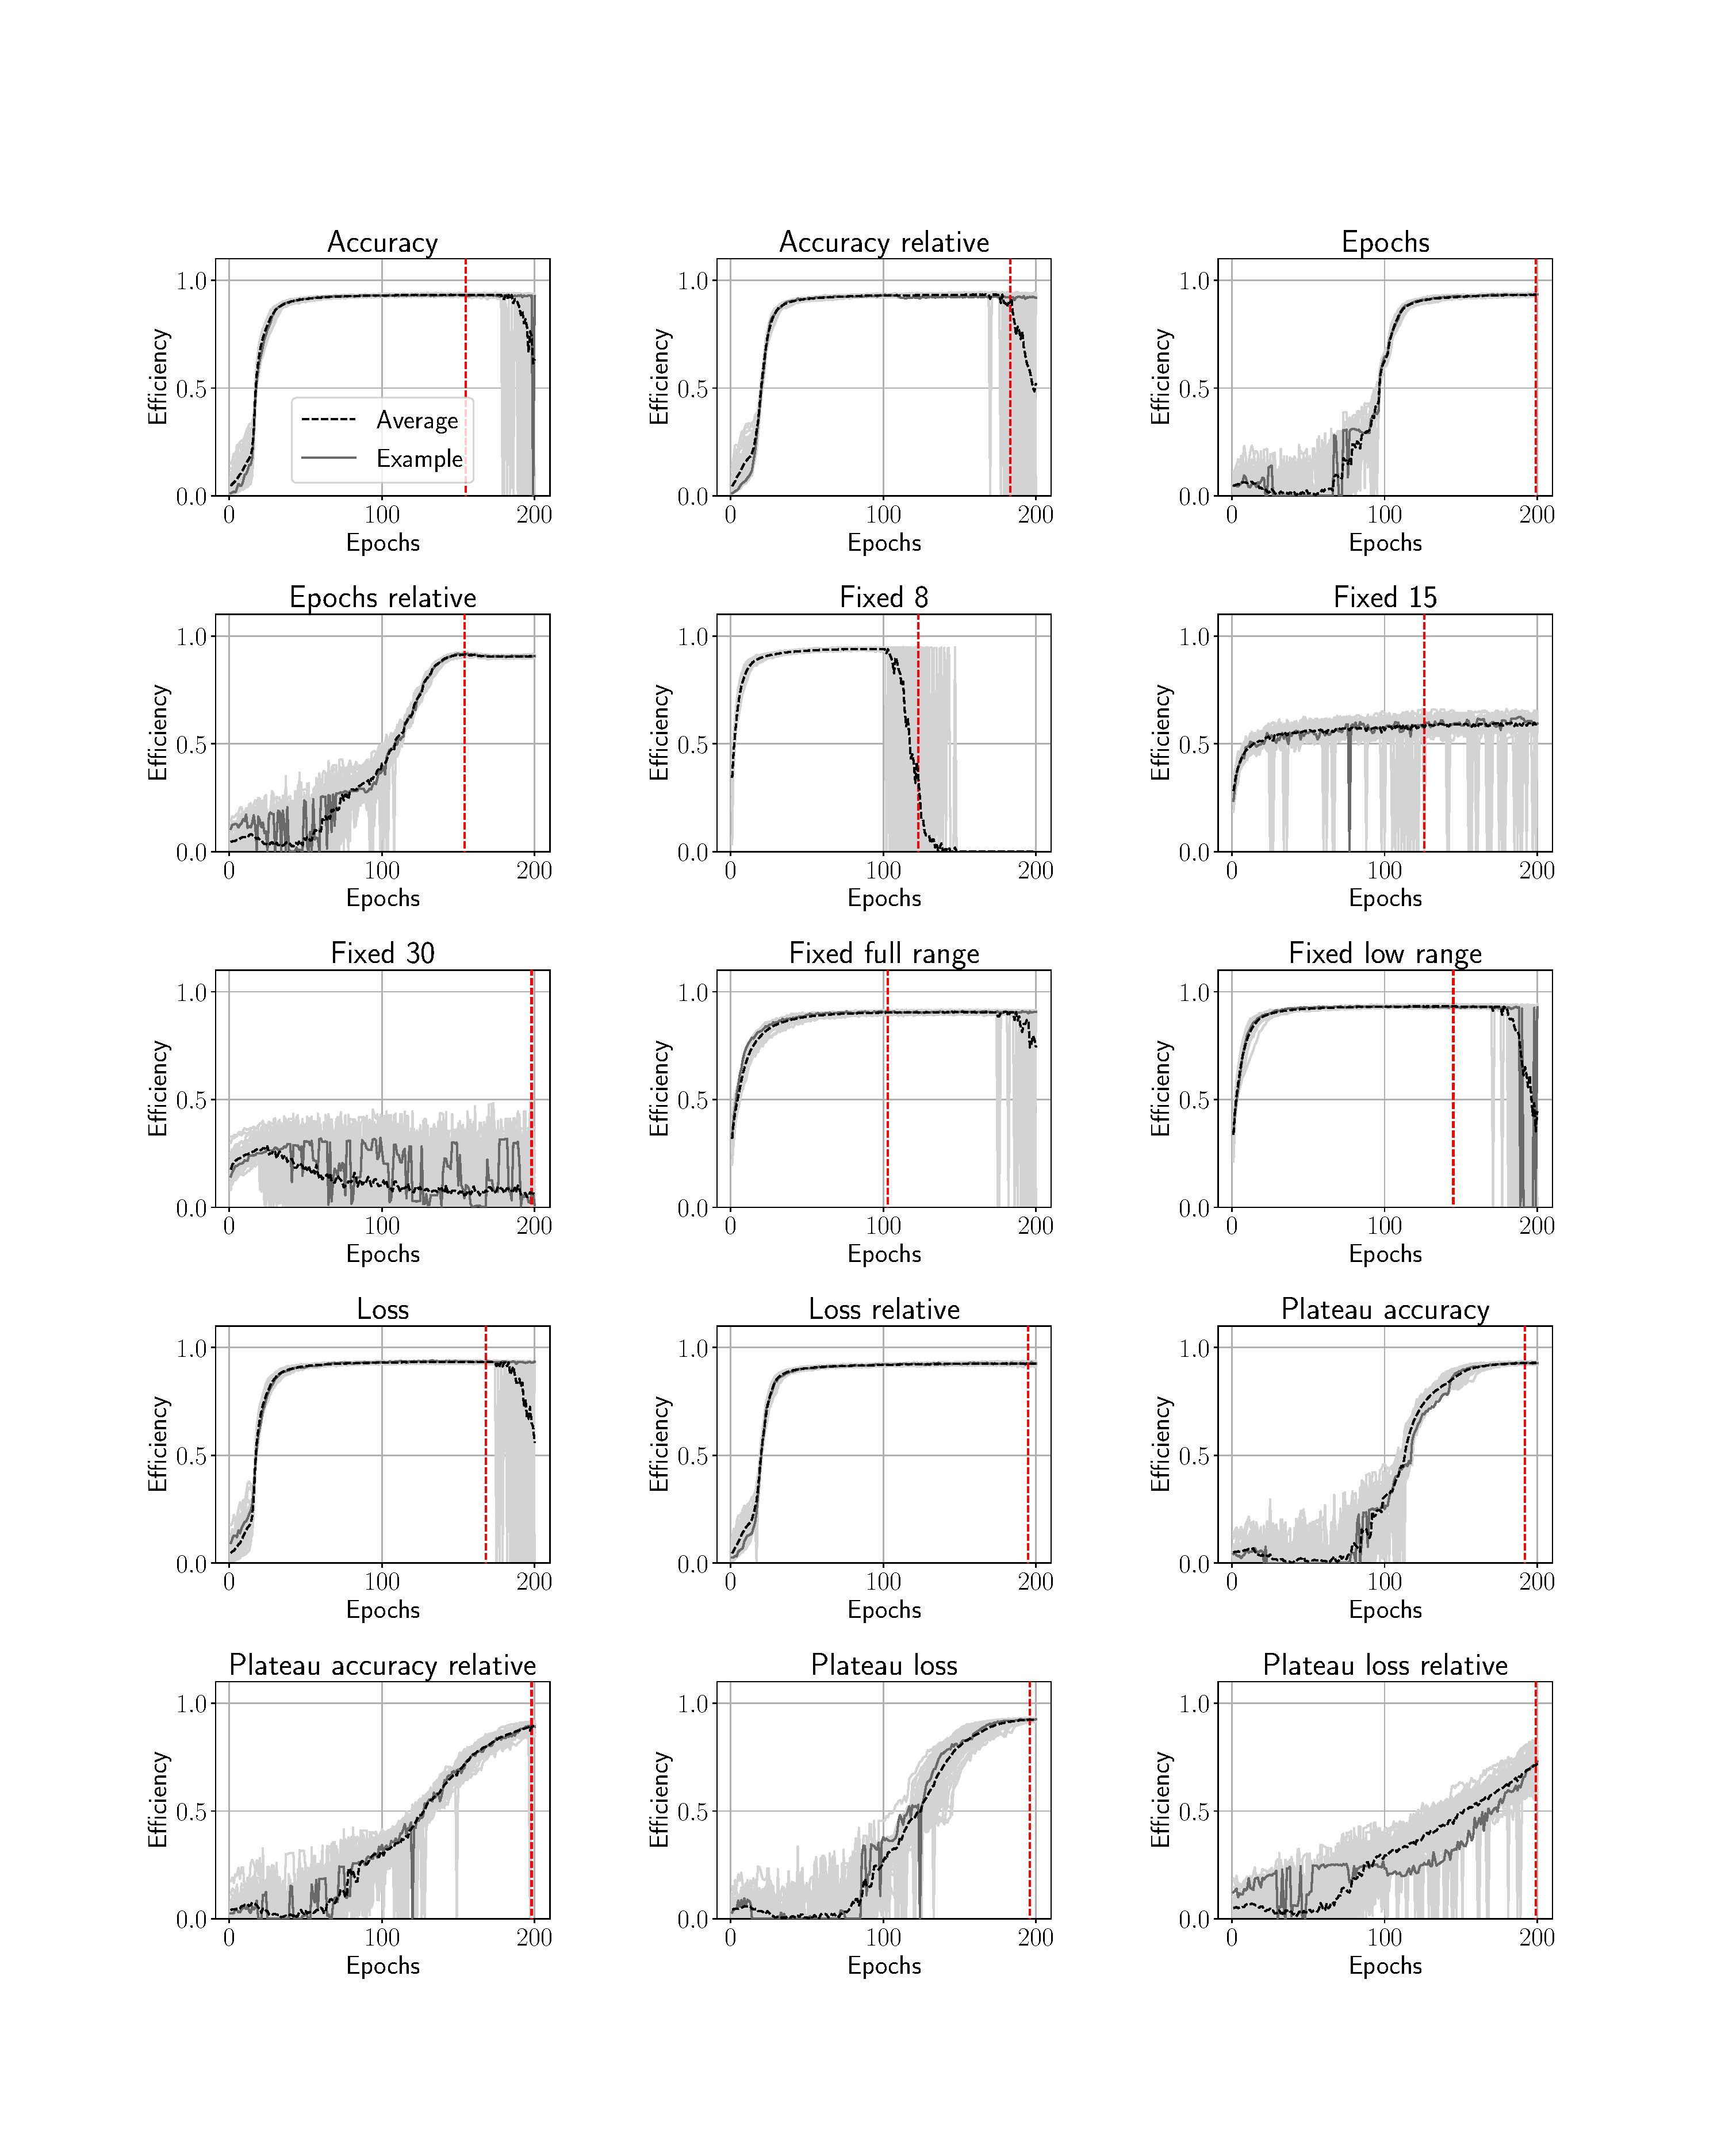
\includegraphics[width=0.95\textwidth, trim=2.5cm 5cm 2.5cm 2cm]{chapters/training_strats/images/overview_softmax.pdf}
    \caption[Network efficiency with Softmax overview]{The efficiency for all $15$ tested training strategies as a function of the training epochs at \acrshort{snr} $9$ and a \acrshort{fap} of $10^{-4}$. The light grey curves show the efficiency for the $50$ independent initialized training runs. The black dashed line shows the average over these individual runs. We highlight the evolution of a single run in dark grey. The vertical, red, dashed line signifies the epoch with the largest efficiency. We choose $3$ networks at this epoch for which to calculate the sensitive volume.}
    \label{fig:efficiency_evolution_all}
\end{figure*}

Most training strategies do not have a major impact on the maximum efficiency. With the exception of training with a fixed \acrshort{snr} $15$ and $30$ all converged networks reach efficiencies of $90\%$ (''Fixed full range'') to $94\%$ (''Fixed 8''). At \acrshort{snr} $6$ the efficiency consistently drops to $24\%$ (''Fixed full range'') to $33\%$ (''Loss relative'') for all converged networks other than the above mentioned exceptions. Above an \acrshort{snr} of $12$ the efficiencies reach $100\%$ for all networks except ''Fixed 15'' and ''Fixed 30''. Those only achieve $100\%$ efficiency at \acrshort{snr} $15$ and $21$ respectively.

The relative plateau strategies did not manage to converge within the first $200$ epochs. For these, we have extended the training length to $400$ epochs, which has allowed these runs to converge. They have reached comparable efficiencies to those mentioned above.

The main difference between all runs is the number of epochs required to reach a converged state. One can see that strategies which supply low \acrshort{snr} signals earlier reach their maximal efficiency earlier. This is especially emphasized with the runs ''Fixed 8'', ''Fixed full range'' and ''Fixed low range''. The curriculum strategies that use the accuracy or loss as their condition also converge quickly. They too supply low \acrshort{snr} samples very early on, as the respective condition is fulfilled at each of the first few epochs. Waiting for a set number of epochs to pass hinders the ability of the network to see low \acrshort{snr} signals early on and, therefore, takes more time to converge. The slowest converging strategies wait for the loss or accuracy to stop improving. They effectively have to wait at least $6$ epochs before lowering the training range. Using a relative approach to lowering the \acrshort{snr} range further decreases the speed at which low \acrshort{snr}s are explored. In the most extreme cases the networks do not converge within the given number of epochs.

Finally, some training strategies become unstable toward the end. All of these unstable strategies converge relatively fast. This suggests that the longer one trains a converged network the more likely the efficiency is to collapse. We, therefore, expect that strategies where the efficiency did not collapse during the first $200$ epochs would see a similar problem during later epochs.

The breakdown of the efficiency was resolved by the \acrshort{usr} modification in \autoref{sec:results:sensitivities}. \autoref{fig:efficiency_evolution_all_lin} shows the evolution of the efficiency at \acrshort{snr} $9$ when this fix is applied. We find that the drops to zero efficiency are removed but the qualitative features of the efficiency curves stay the same.

\begin{figure*}
    \centering
    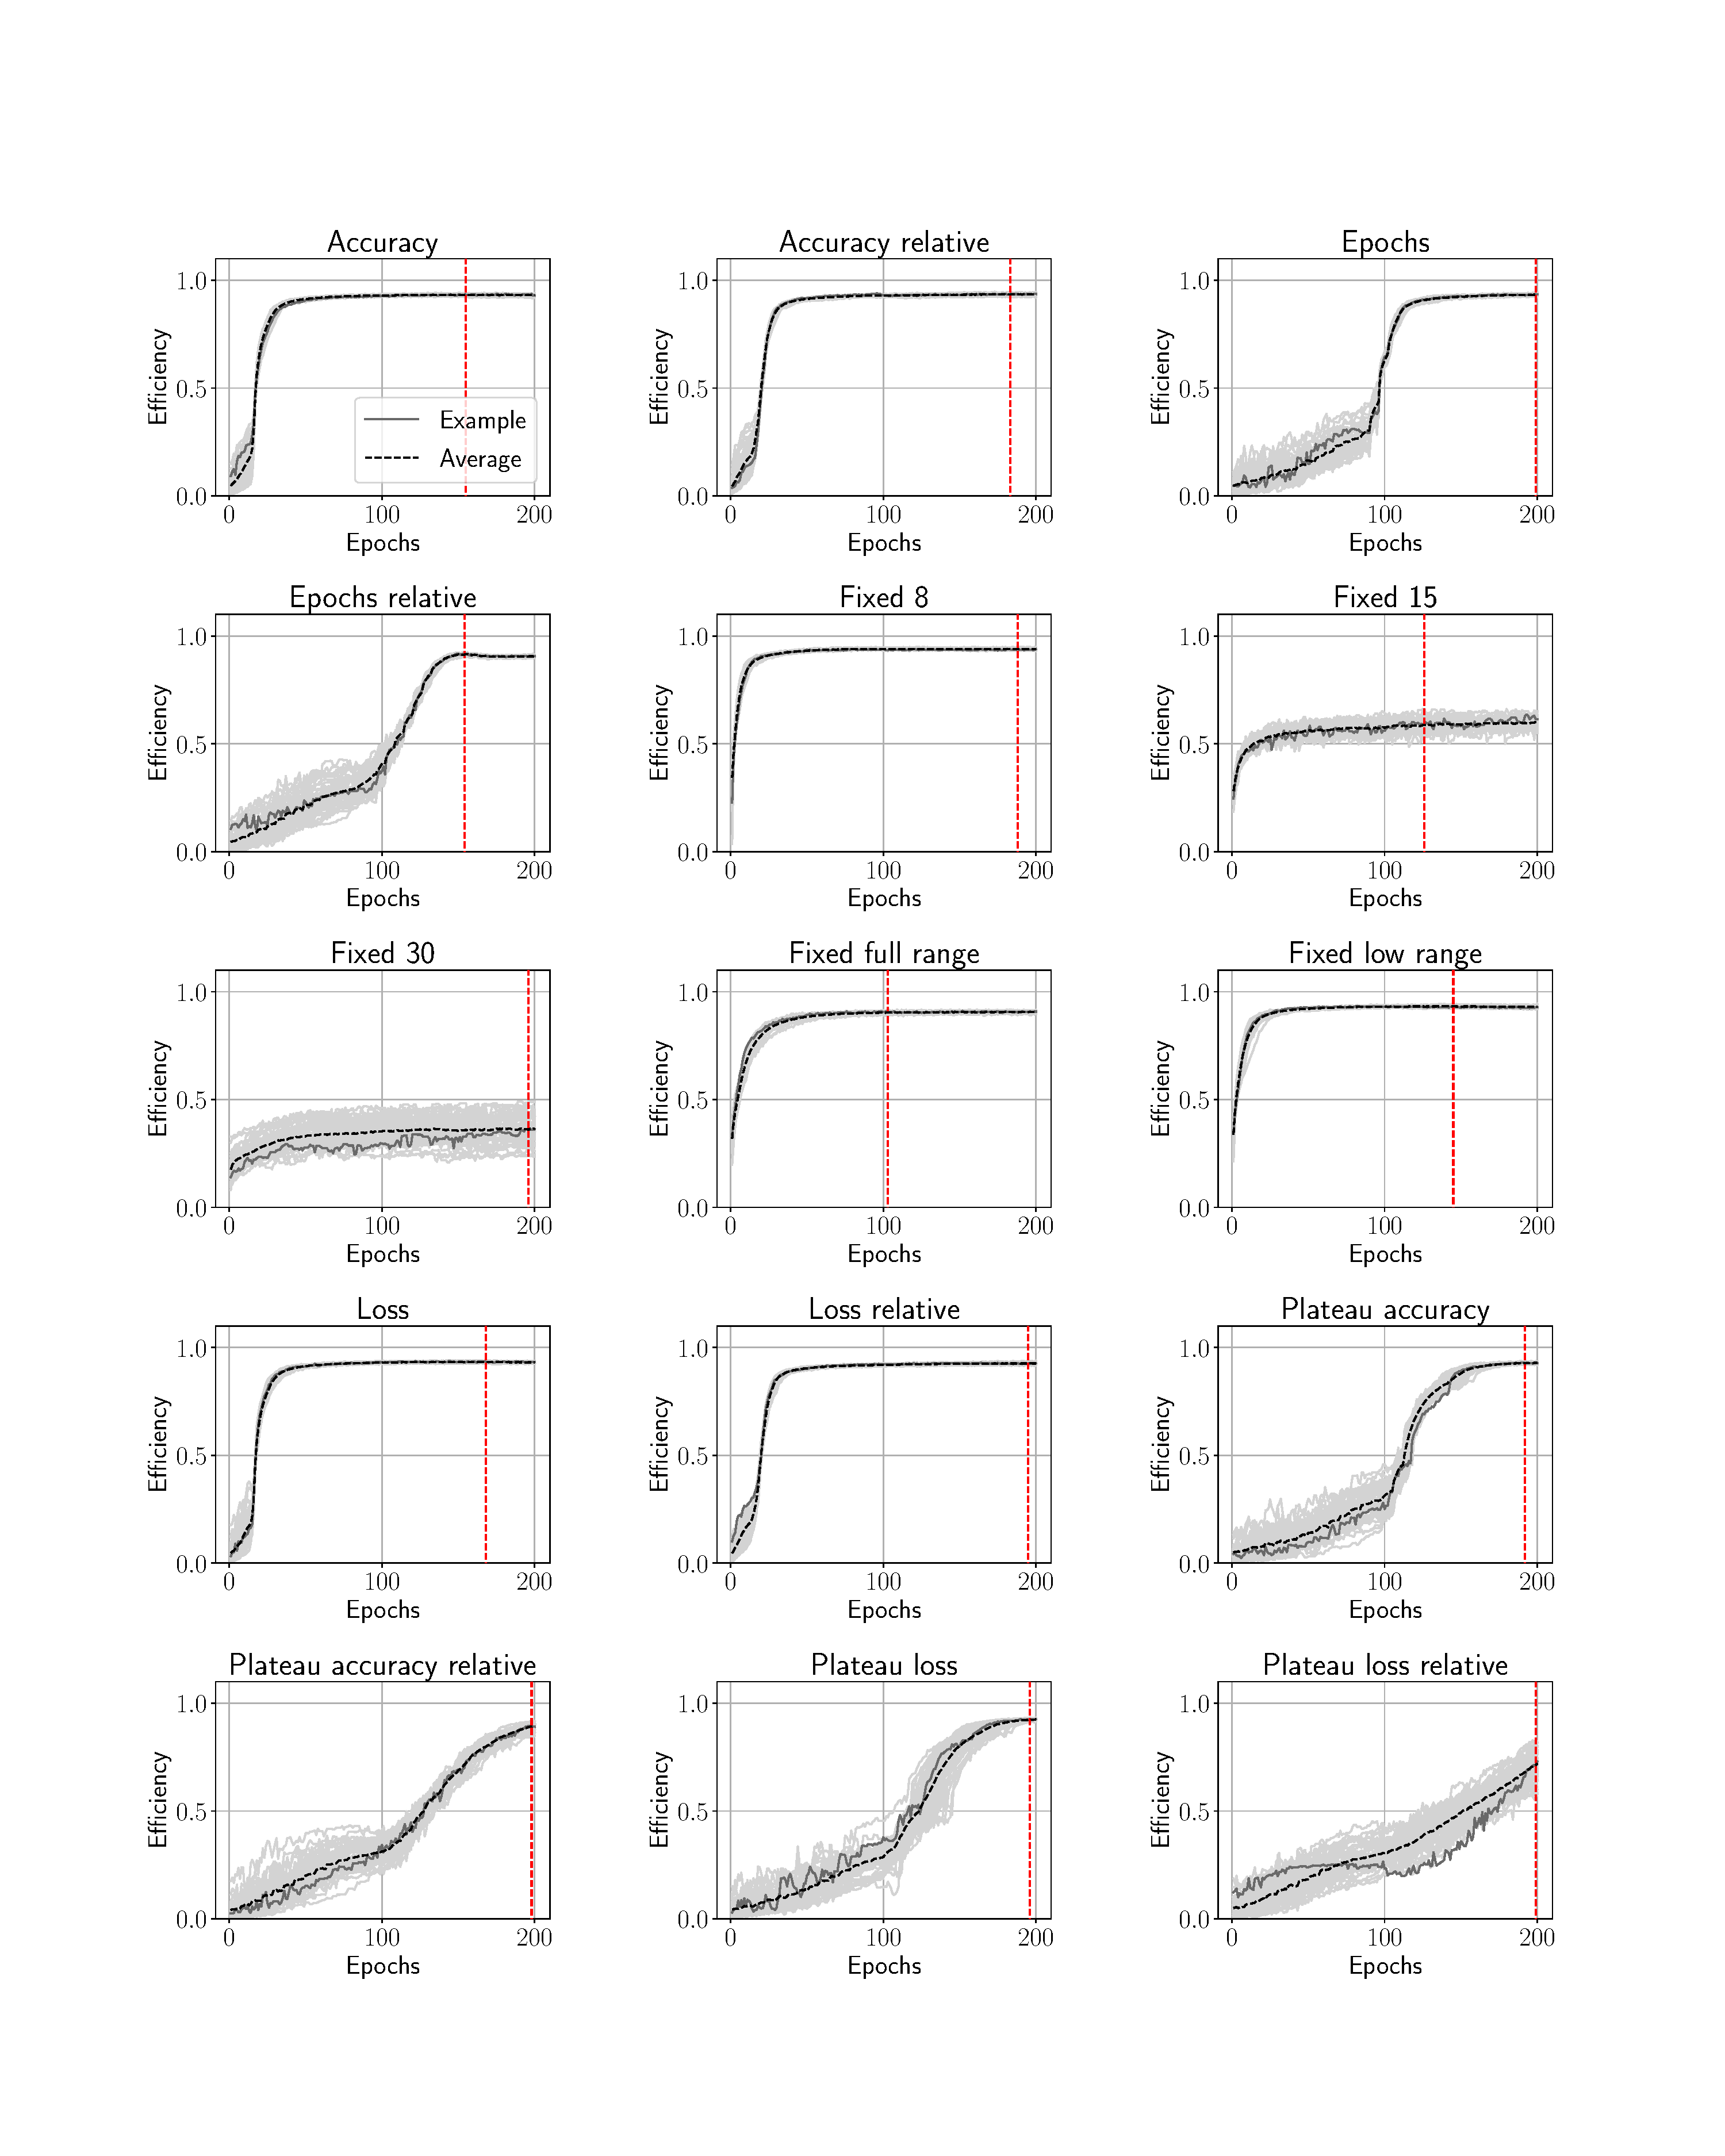
\includegraphics[width=0.95\textwidth, trim=2.5cm 5cm 2.5cm 2cm]{chapters/training_strats/images/overview_linear.pdf}
    \caption[Network efficiency with unbounded Softmax replacement overview]{The efficiency for all $15$ tested training strategies as a function of the training epochs at \acrshort{snr} $9$ and a \acrshort{fap} of $10^{-4}$. The light grey curves show the efficiency for the $50$ independent initialized training runs. The black dashed line shows the average over these individual runs. We highlight the evolution of a single run in dark grey. The vertical, red, dashed line signifies the epoch with the largest efficiency. We choose $3$ networks at this epoch for which to calculate the sensitive volume. This figure shows the same networks as \autoref{fig:efficiency_evolution_all} with the \acrshort{usr} modification applied. With this modification the efficiency stays $>0$ at all times.}
    \label{fig:efficiency_evolution_all_lin}
\end{figure*}

All efficiency plots were generated from the TensorFlow version of the networks. When training with PyTorch we found the results virtually indistinguishable from the TensorFlow version.

We repeated our tests on networks with different capacities, although this was not the main focus of the present work, to ensure that our findings are robust against a few specific architecture changes. We found no significant differences in the final efficiency, although the speed of training convergence varied. Such studies are left to future work.

\section{Conclusions}\label{sec:conclusion}
In this paper, we revisited the first deep learning \acrshort{gw} search algorithms and compared them directly to a matched-filter search. We showed that for the considered parameter space and for a single detector the networks retain performance closely following matched filtering even on long duration continuous data sets and when considering \acrshort{far} thresholds down to once per month. While there are now more sophisticated deep learning algorithms available that enhance the capabilities of the first proofs of concept, we think that there is still a lot to be learned from these first steps.

Our initial focus was the optimization of the data presentation to these networks. Two kinds of training strategies were previously explored; curriculum learning, where training samples become more difficult to classify as training continues, and fixed interval training, where the complexity of the training set stays constant.

We found that the particular strategy is of little importance to the eventual performance of the network. It depends a lot more on the presence of sufficiently complex samples in the training set. In particular, we found that the networks are able to generalize low \acrshort{snr} signals to high \acrshort{snr} ones but not vice versa.

On the other hand, the training strategy does have an impact on the time it takes the network to converge. Since high \acrshort{snr} examples are not as important to the performance of the network, strategies that provide low \acrshort{snr} samples earlier converge faster. In conclusion, we recommend training deep learning search algorithms on a fixed range of low \acrshort{snr} signals.

We use efficiency as our metric of performance during training. As this statistic has been used in previous publications, it allows us to verify that we have converged to the expected performance.

The efficiency at \acrshort{fap}s $\leq 10^{-4}$ dropped to zero when networks were trained for extended periods of time. This was unexpected and limited our ability to test the search.

We found the drops in efficiency to be caused by numerical instabilities in the final activation function of the networks. By removing the Softmax activation on the final layer and imposing thresholds directly on the linear output of the network, we were able to lift the limitations on the testable \acrshort{fap}s. This \acrshort{usr} modification has proven to be simple and effective, as no re-training of the networks is required and virtually unlimited low \acrshort{fap}s can be tested.

To compare the deep learning based searches to an equivalent matched-filter search we calculated the sensitive volumes as functions of the \acrshort{far}s on a month of simulated data. We found that the machine learning algorithm is able to closely follow the performance of the traditional algorithm even down to \acrshort{far}s of 1 per month, when \acrshort{usr} is used.

The results given here are limited to a single detector, Gaussian noise and signals from \acrshort{bbh}s, which are relatively short in duration and comparatively simple to detect with existing methods. Parts of the parameter space, like the inclusion of higher-order modes \cite{Harry:2017weg}, eccentricity \cite{Nitz:2019spj}, or precession \cite{Harry:2016ijz}, where current searches are computationally limited, are not yet included. However, it is expected that neural networks may generalize efficiently to these more difficult signals. Deep learning detection algorithms for spinning black holes with precession were recently explored for the first time by \cite{Wei:2020ztw}. There is also ongoing work to construct neural network searches targeting long duration signals \cite{Dreissigacker:2020xfr, Krastev:2019koe, Schafer:2020kor, Wei:2020sfz}. Considering real noise may enable deep learning algorithms to outperform matched filtering, which is only known to be optimal for stationary Gaussian noise. Multiple studies have shown that neural networks adapt well to non-stationary noise contaminated with glitches \cite{George:2017pmj,Wei:2020sfz,Wei:2020ztw,Yan:2021wml}.


\section{Appendix: Efficiency curve examples}
This appendix provides examples of the usefulness of \acrshort{usr} for various training strategies explored in this paper. The plots show the efficiency as a function of training epochs at 4 distinct \acrshort{snr}s with and without the application of the \acrshort{usr}. For both shown examples the \acrshort{usr} manages to remove the efficiency breakdown entirely.

\begin{figure*}
    \centering
    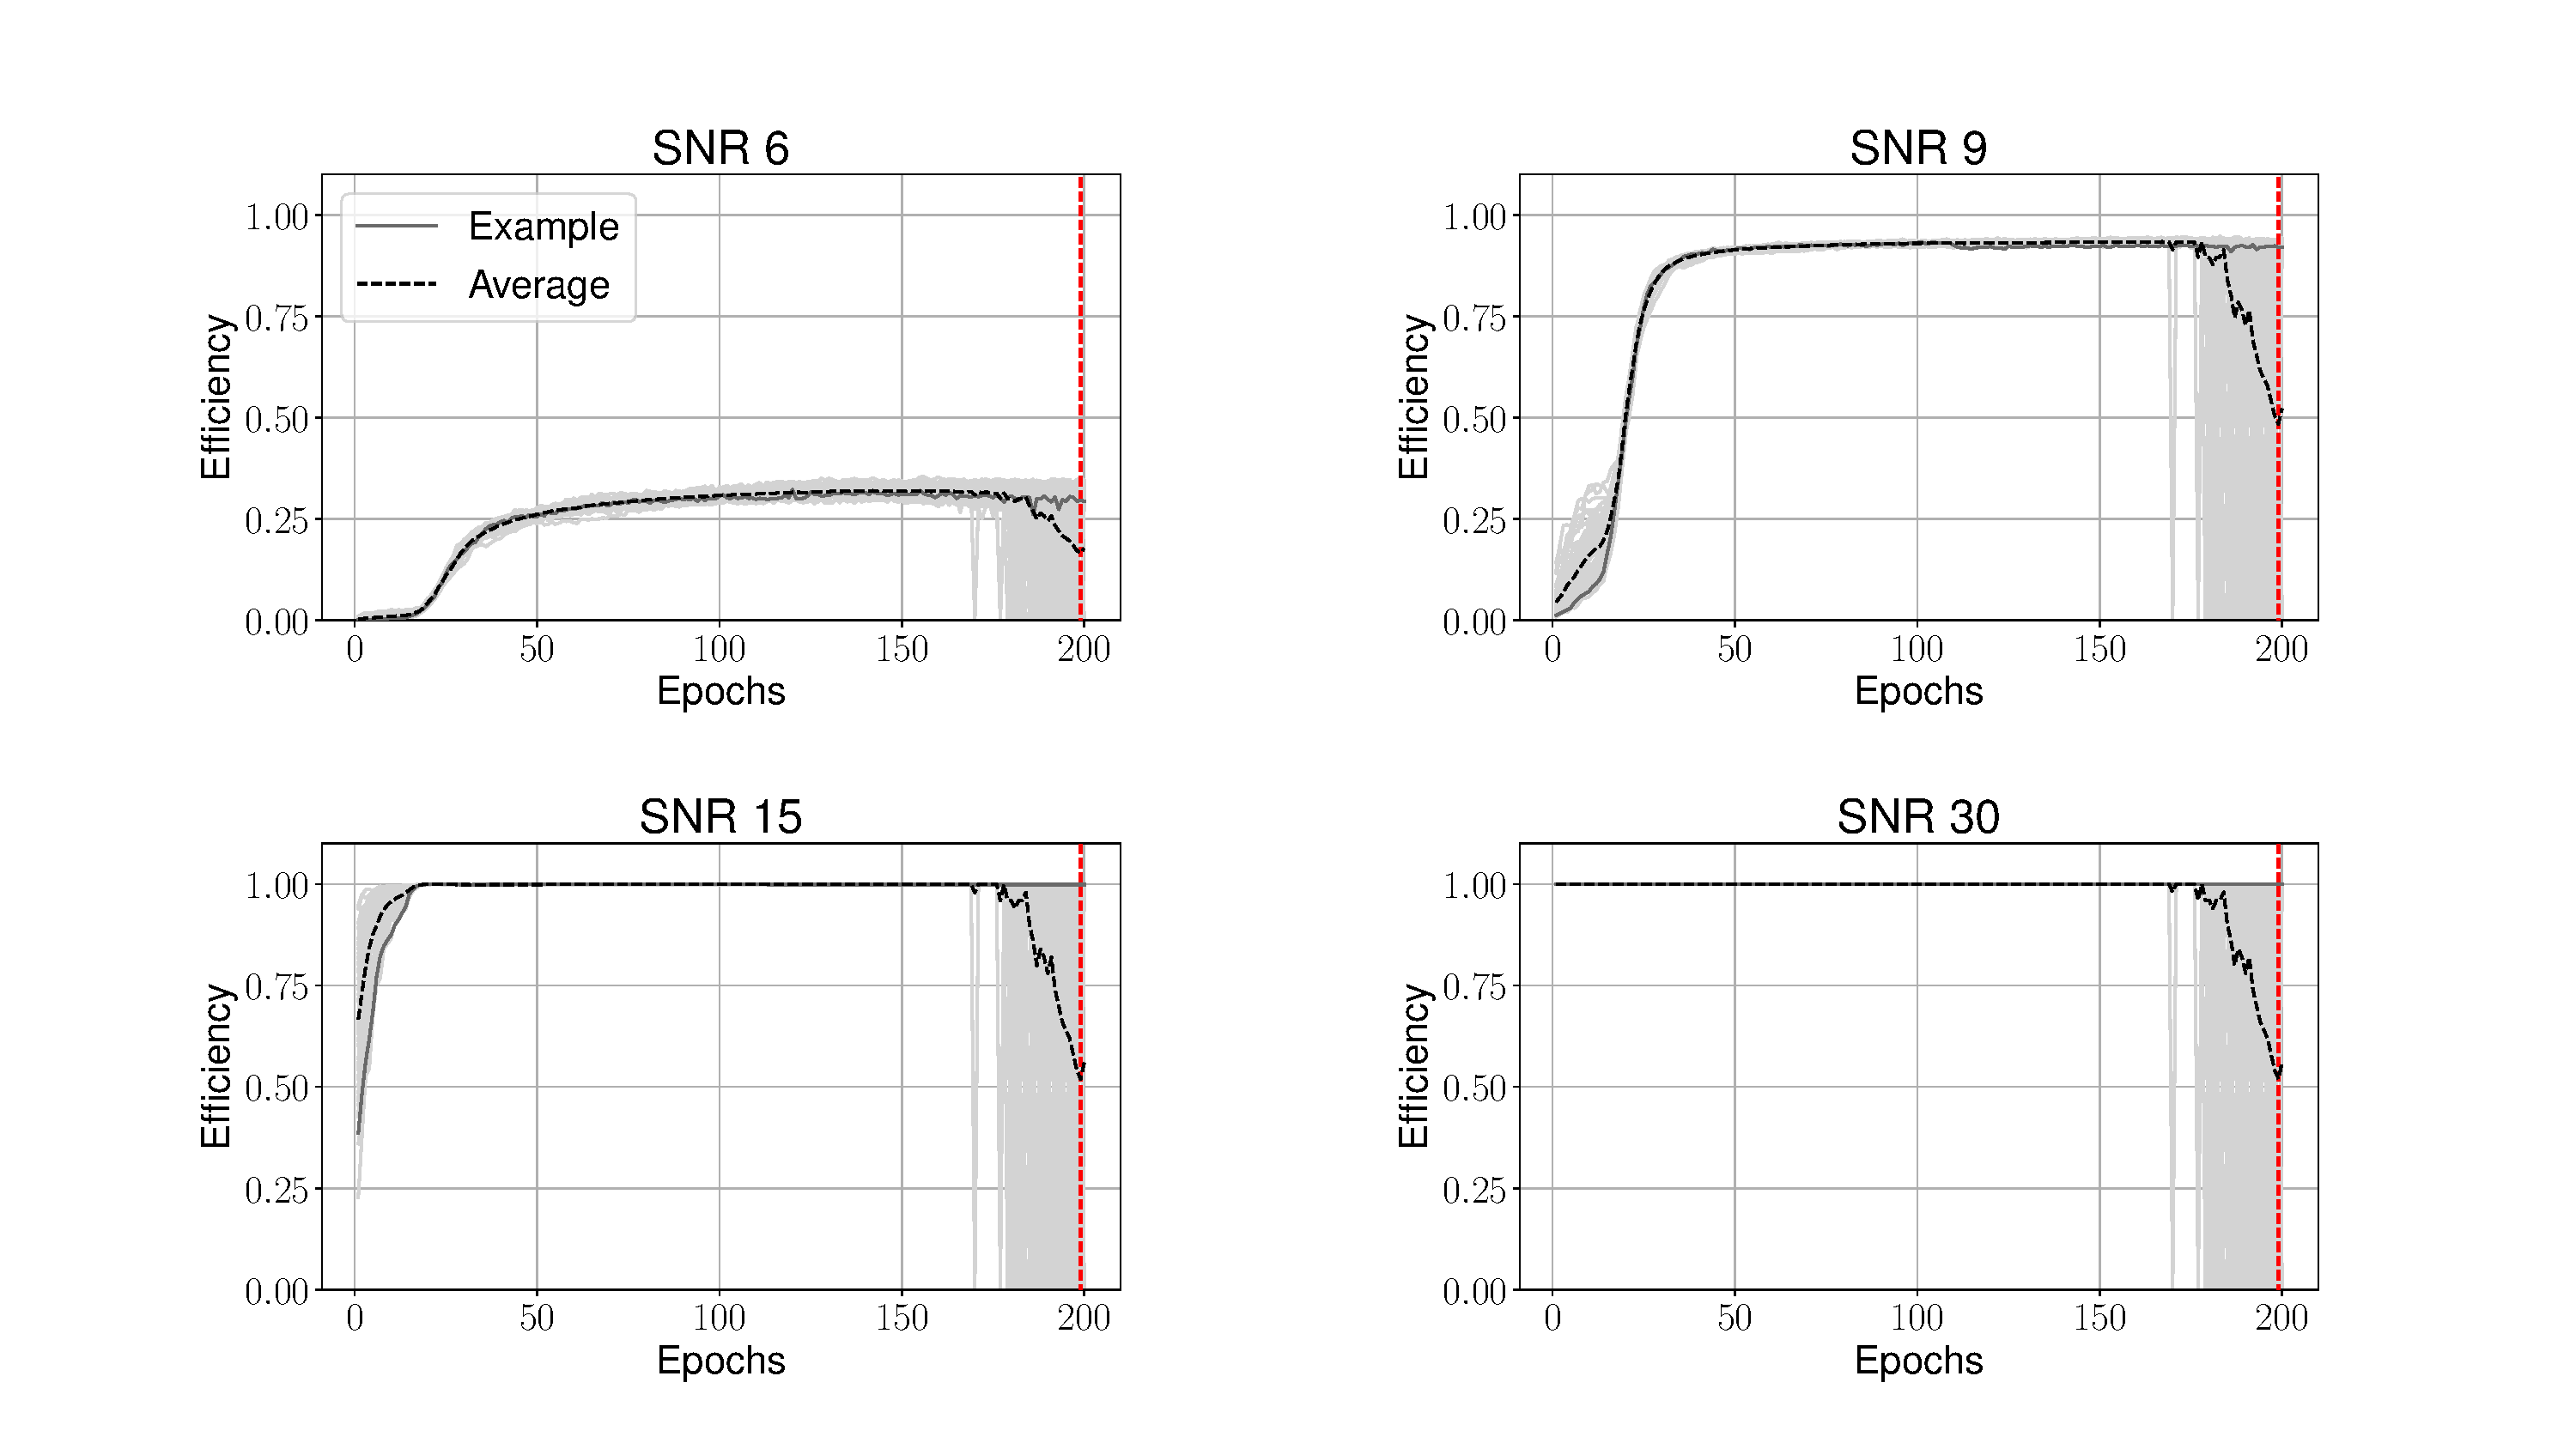
\includegraphics[width=\textwidth]{chapters/training_strats/images/acc_rel_soft.pdf}
    \caption[Efficiency evolution ``Accuracy relative'' using Softmax]{Efficiency evolution of the "Accuracy relative" strategy using the Softmax output as a ranking statistic.}
    \label{fig:efficiency_evolution_acc_rel_soft}
\end{figure*}

\begin{figure*}
    \centering
    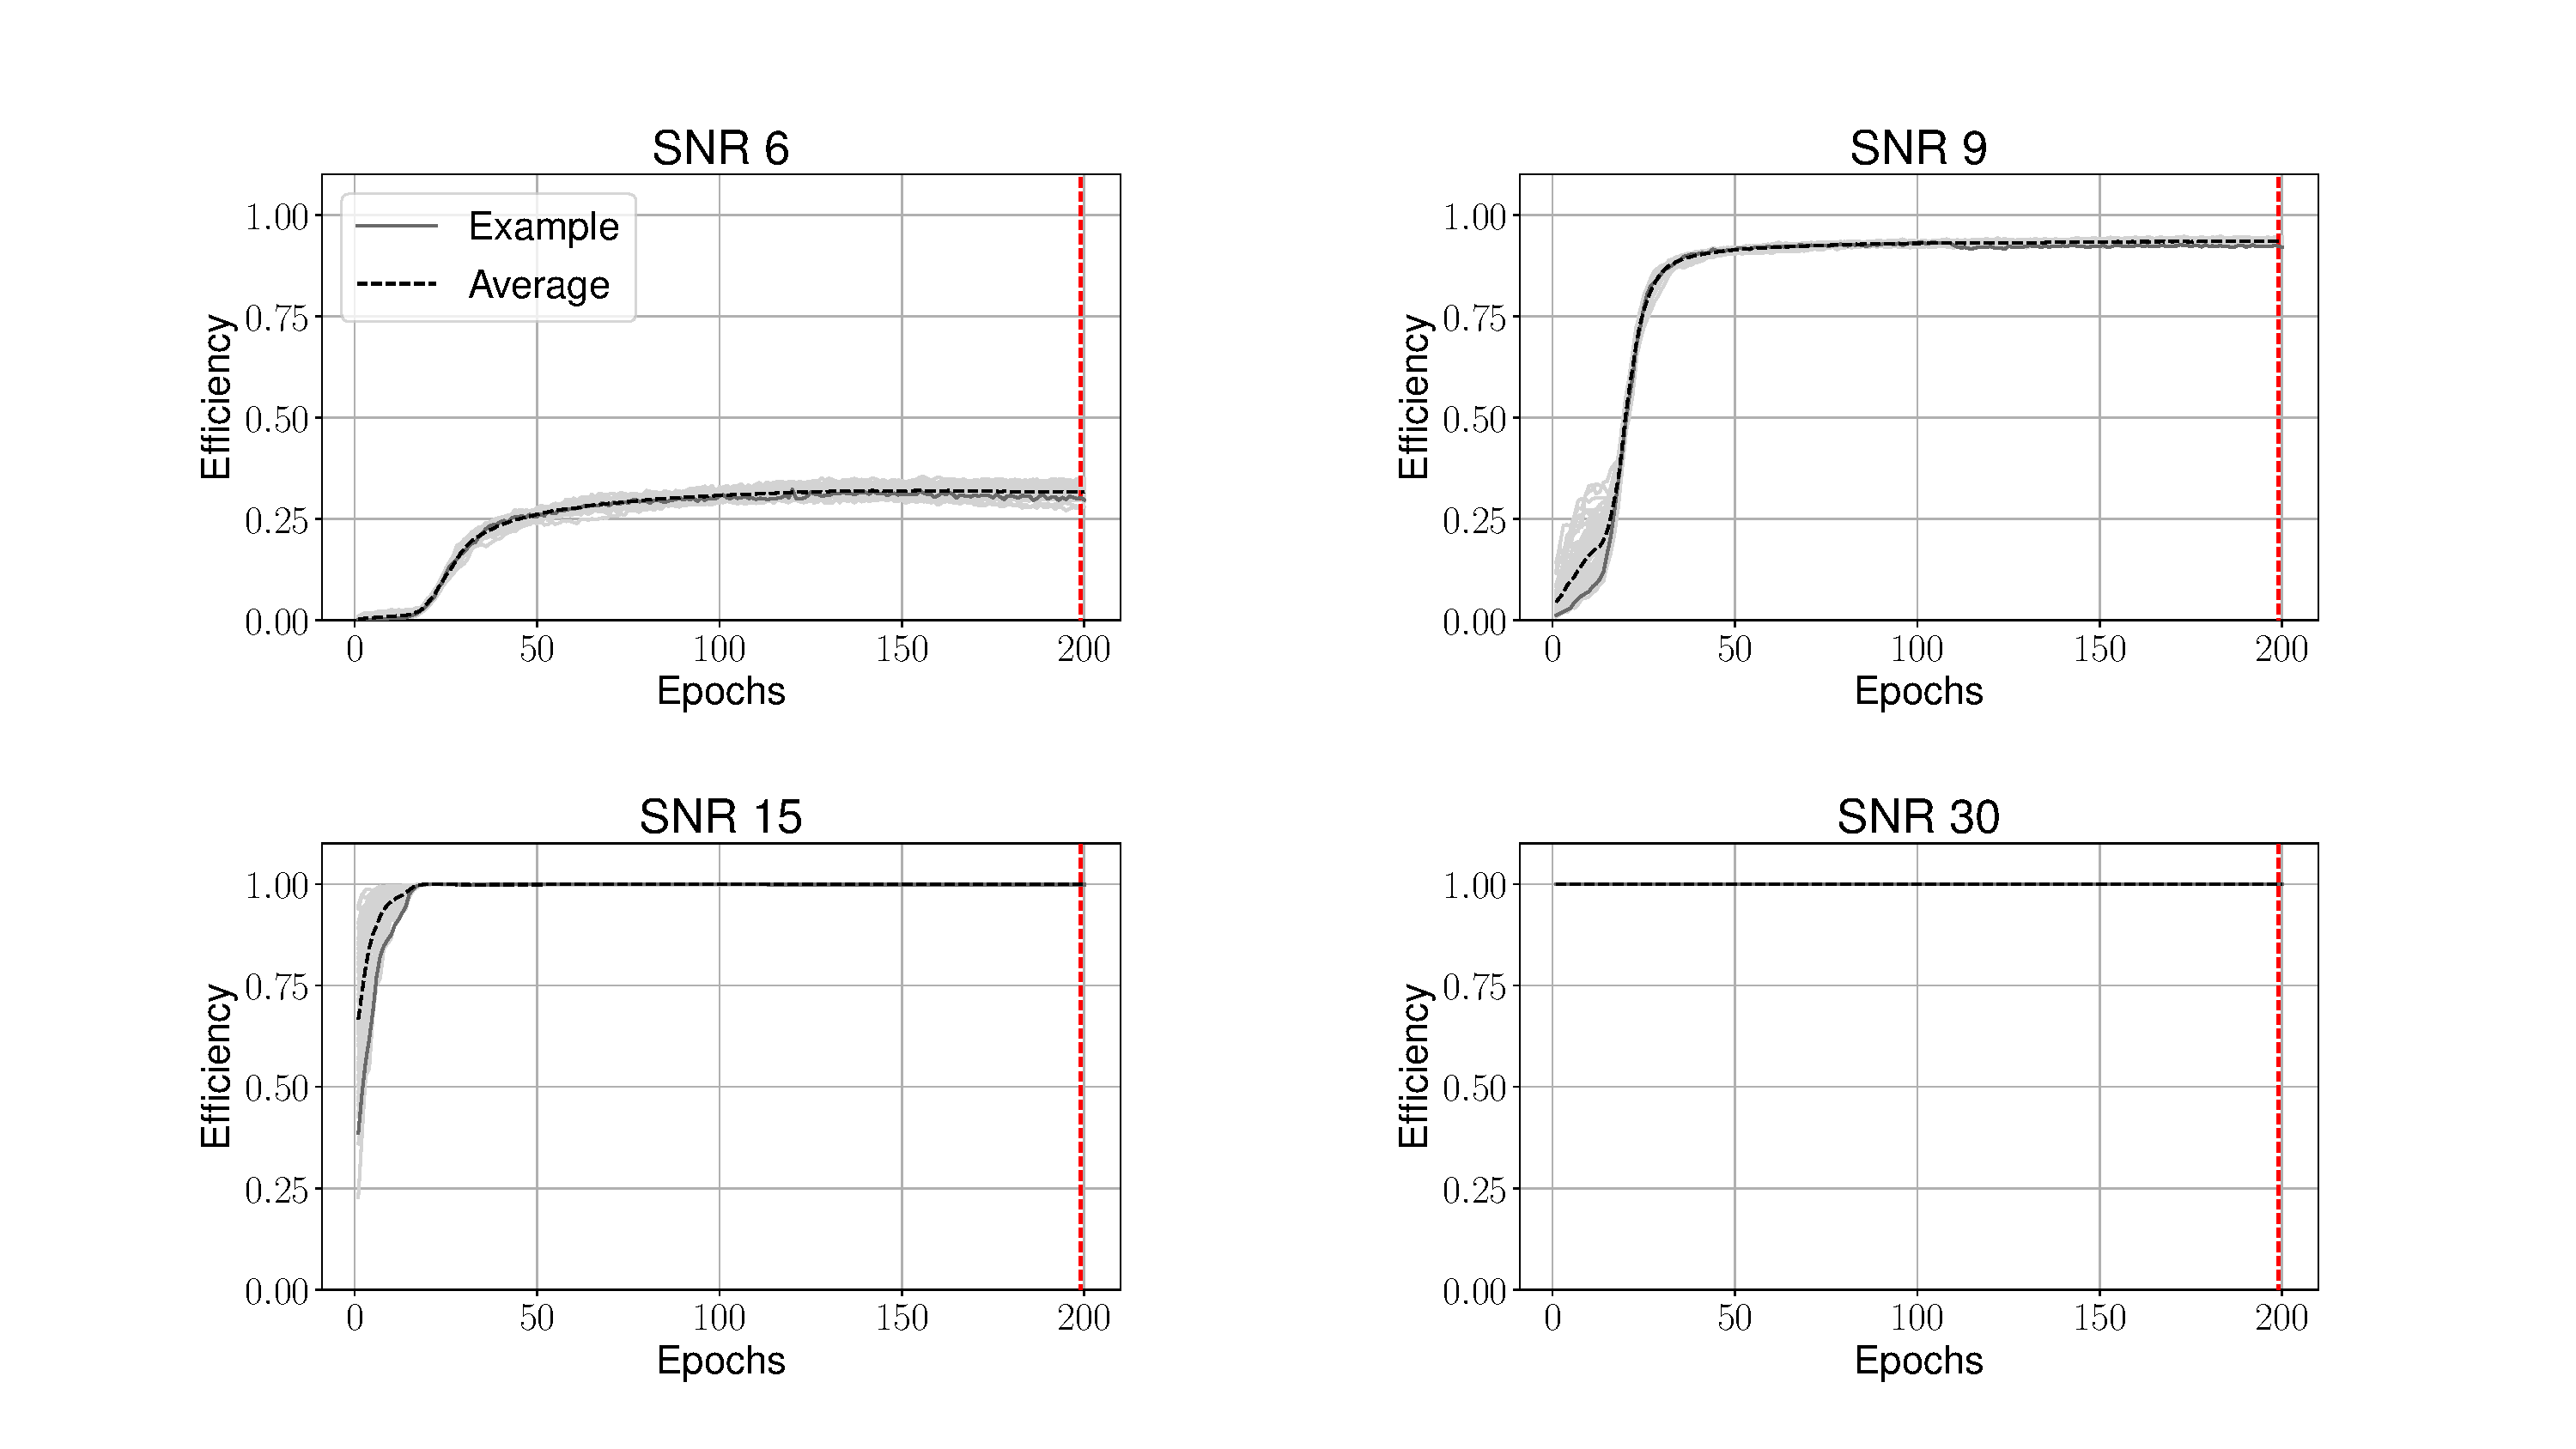
\includegraphics[width=\textwidth]{chapters/training_strats/images/acc_rel_lin.pdf}
    \caption[Efficiency evolution ``Accuracy relative'' using unbounded Softmax replacement]{Efficiency evolution of the "Accuracy relative" strategy using the \acrshort{usr} modification.}
    \label{fig:efficiency_evolution_acc_rel_lin}
\end{figure*}

\begin{figure*}
    \centering
    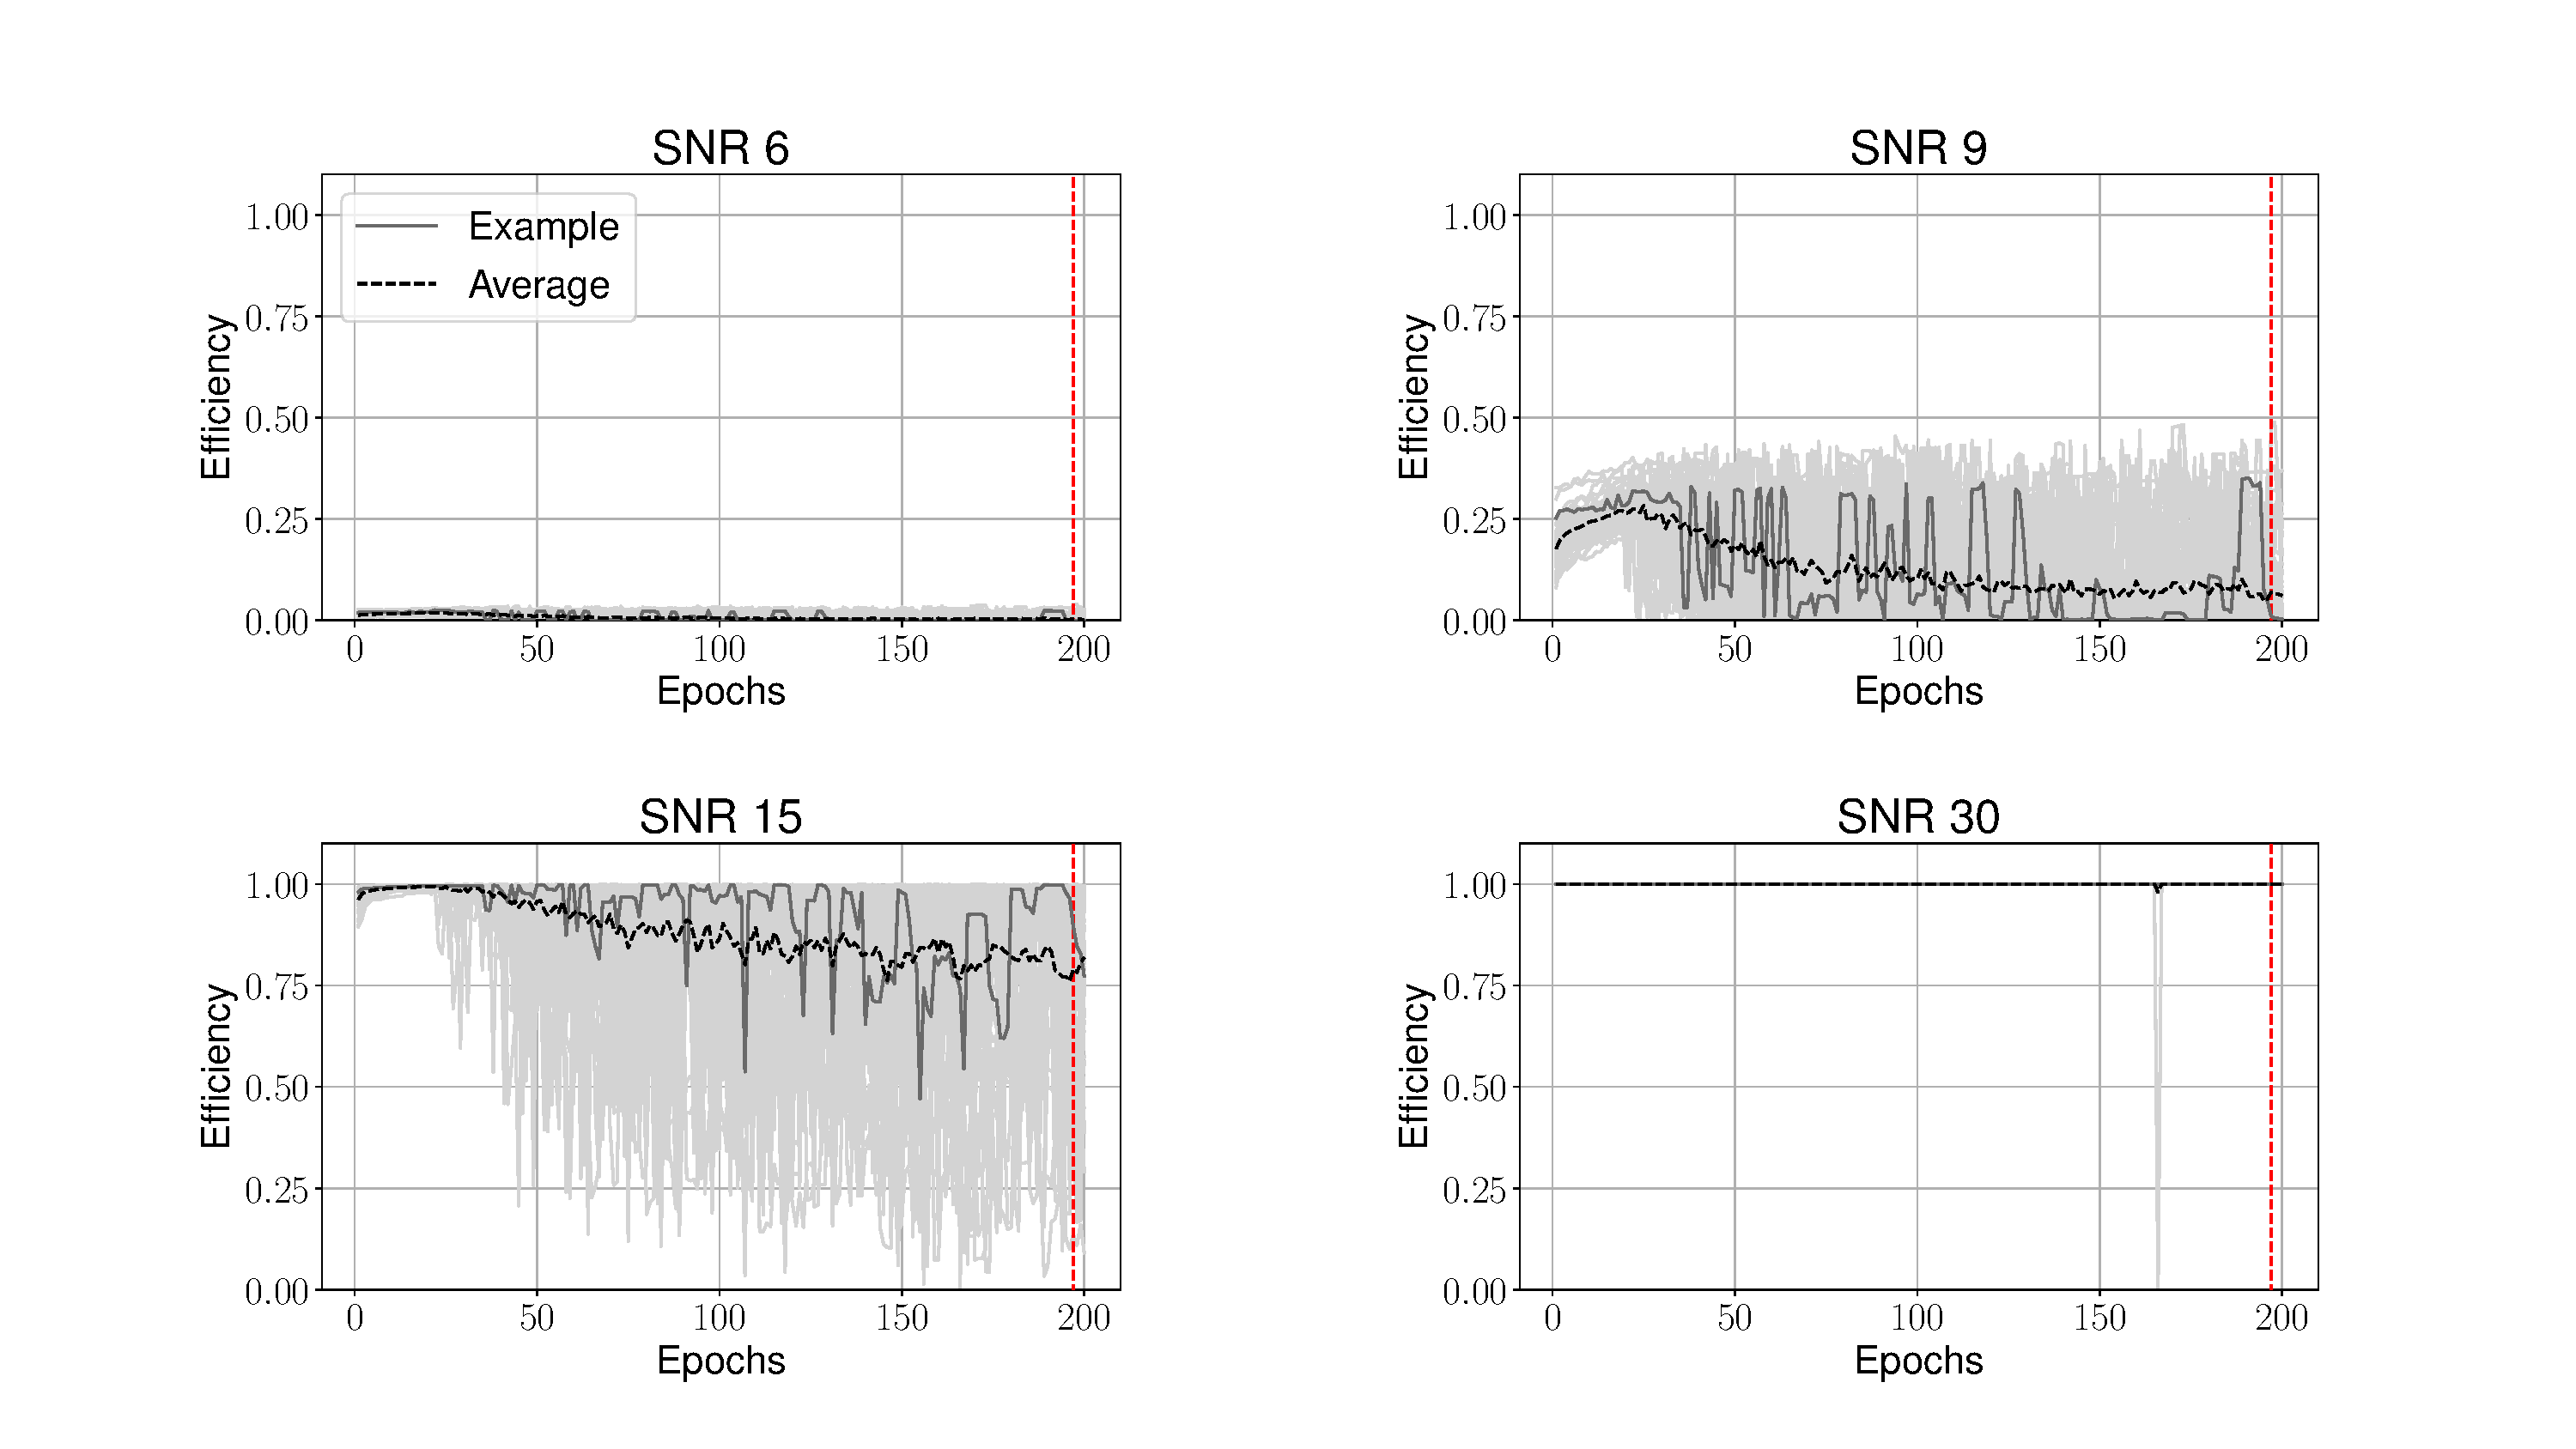
\includegraphics[width=\textwidth]{chapters/training_strats/images/fixed_30_soft.pdf}
    \caption[Efficiency evolution ``Fixed 30'' using Softmax]{Efficiency evolution of the "Fixed 30" strategy using the Softmax output as a ranking statistic.}
    \label{fig:efficiency_evolution_fixed_30_soft}
\end{figure*}

\begin{figure*}
    \centering
    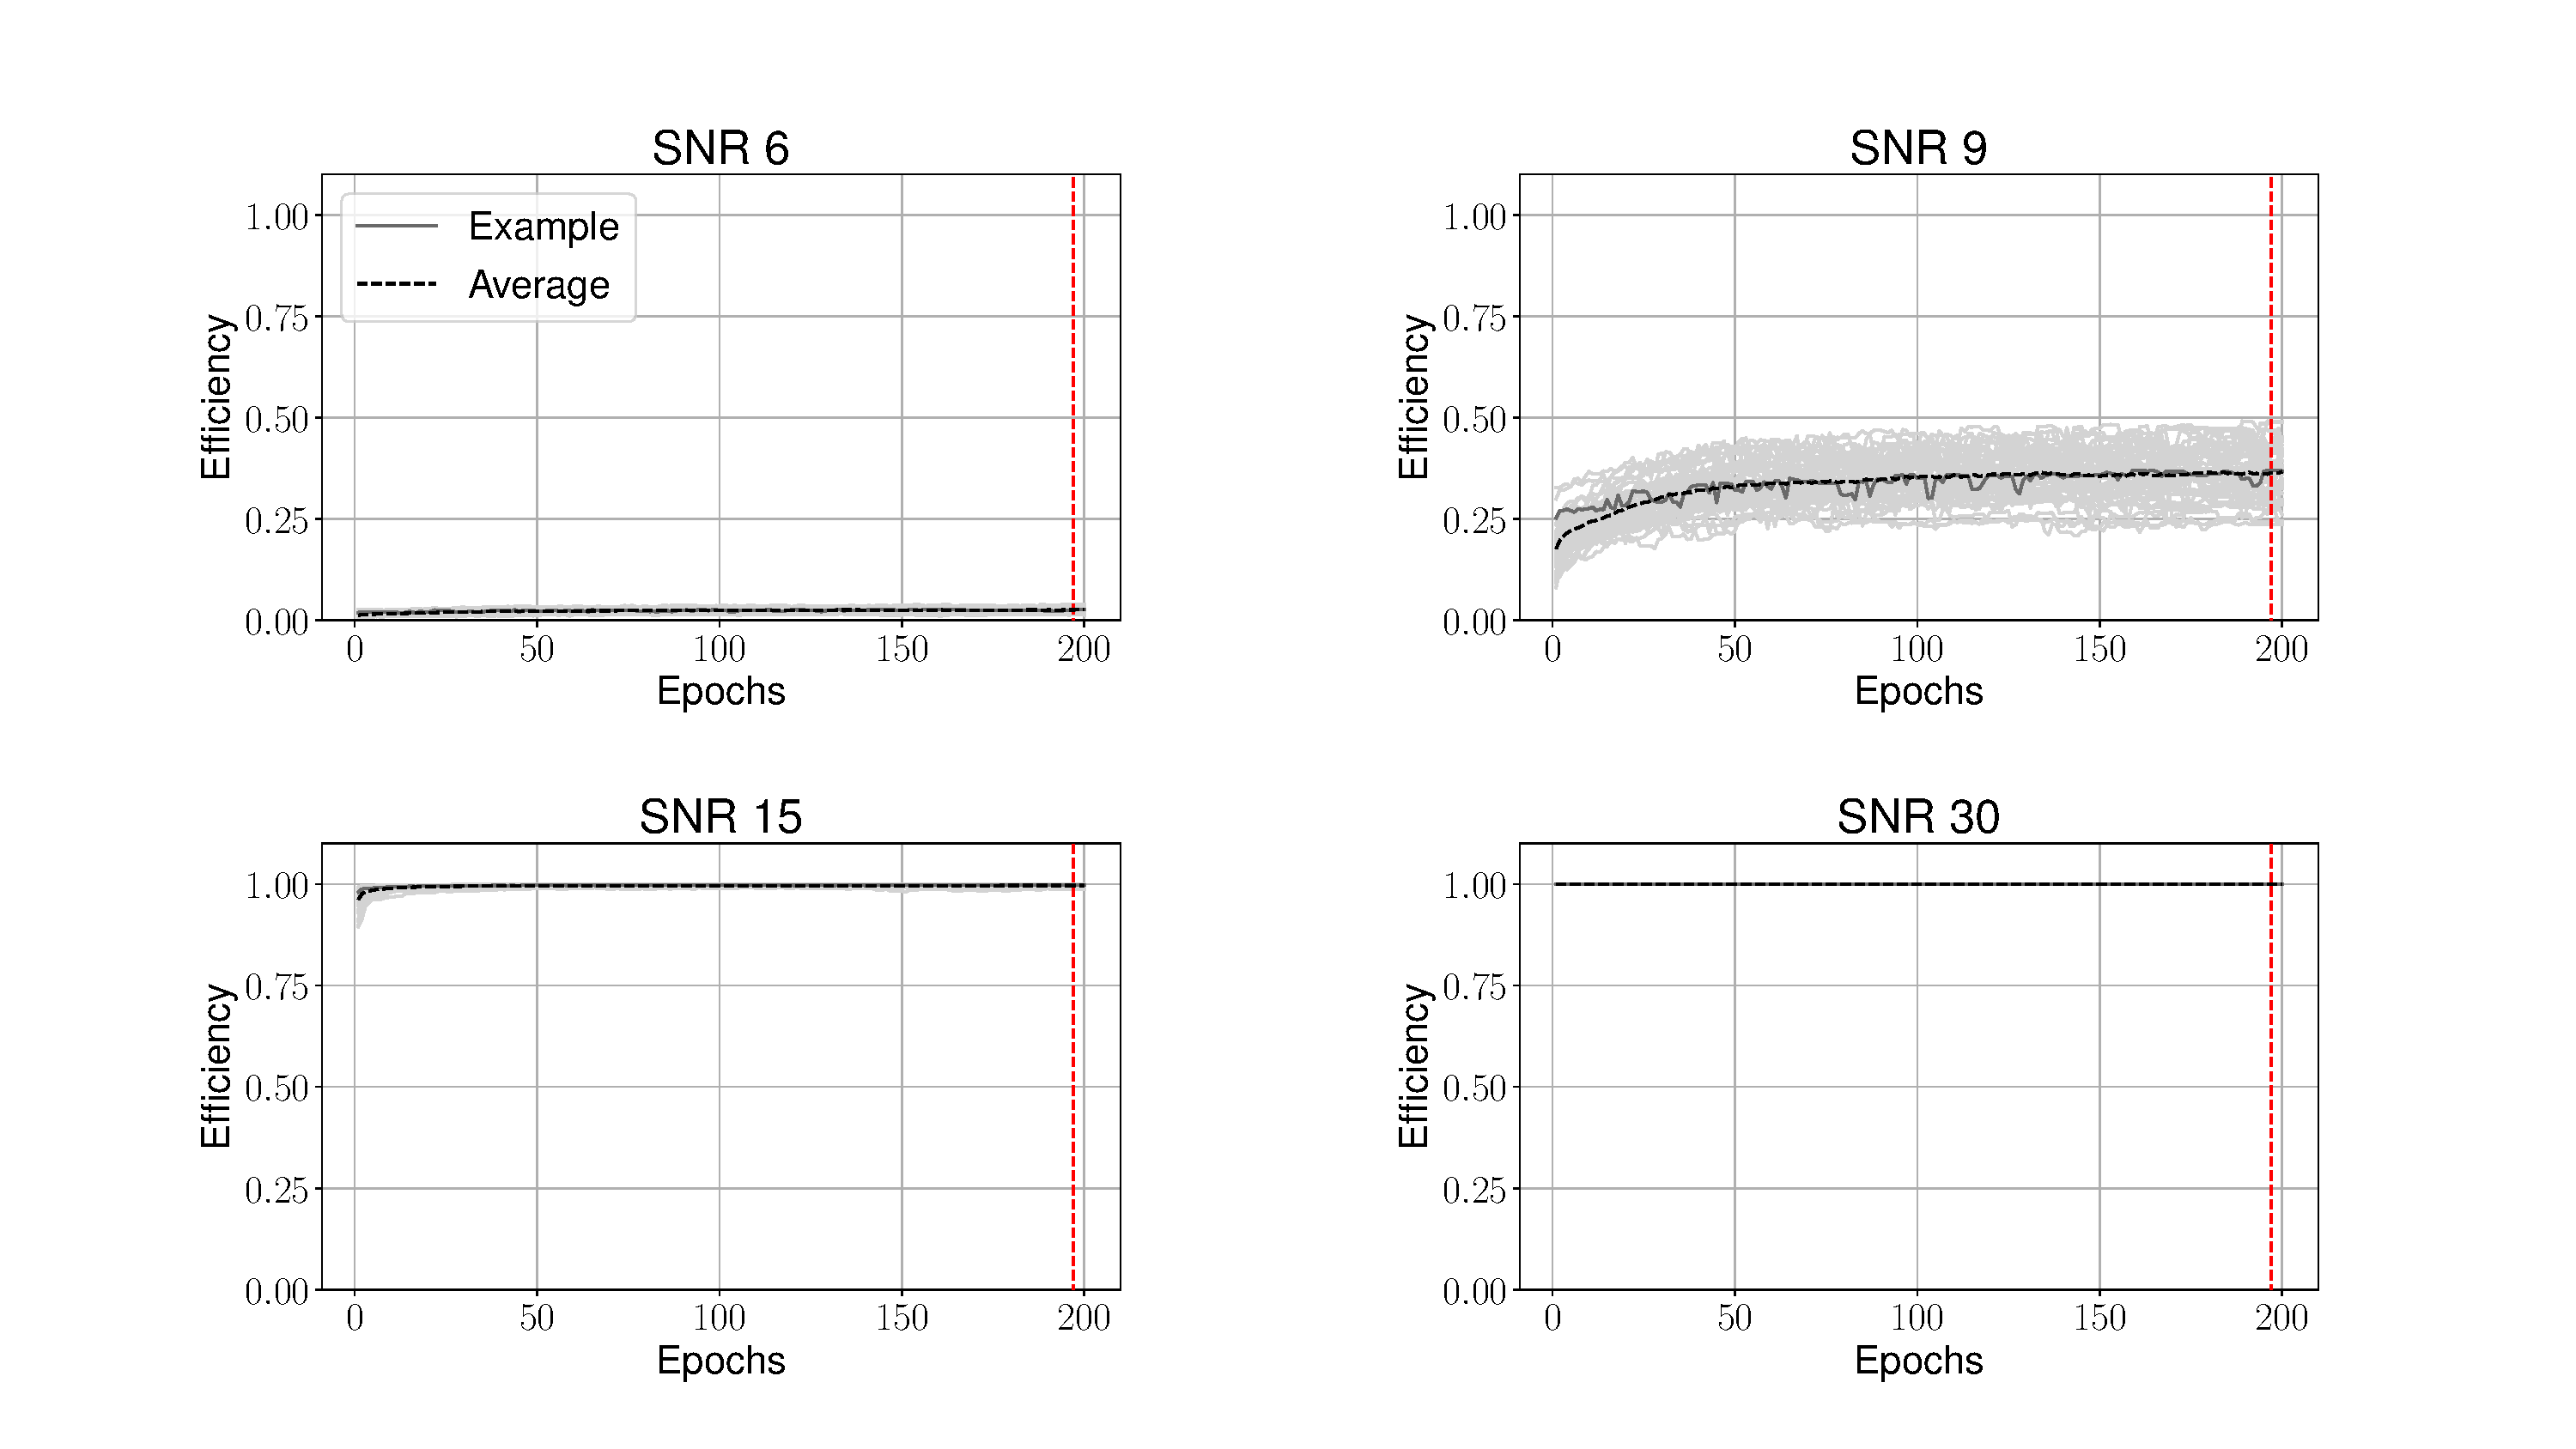
\includegraphics[width=\textwidth]{chapters/training_strats/images/fixed_30_lin.pdf}
    \caption[Efficiency evolution ``Fixed 30'' using unbounded Softmax replacement]{Efficiency evolution of the "Fixed 30" strategy using the \acrshort{usr} modification.}
    \label{fig:efficiency_evolution_fixed_30_lin}
\end{figure*}


\chapter{From One to Many: A Deep Learning Coincident Gravitational-Wave Search}\label{ch:cnn_coinc}
\minitoc
This chapter is essentially a full reprint of \cite{Schafer:2021cml} with some minor edits for formatting. It explores the capability of deep learning \acrshort{gw} search algorithms trained on a single detector to be applied in a coincidence search.

\setcounter{section}{-1}
\section{Abstract}
Gravitational waves from the coalescence of compact-binary sources are now routinely observed by Earth bound detectors. The most sensitive search algorithms convolve many different pre-calculated gravitational waveforms with the detector data and look for coincident matches between different detectors. Machine learning is being explored as an alternative approach to building a search algorithm that has the prospect to reduce computational costs and target more complex signals. In this work we construct a two-detector search for gravitational waves from binary black hole mergers using neural networks trained on non-spinning binary black hole data from a single detector. The network is applied to the data from both observatories independently and we check for events coincident in time between the two. This enables the efficient analysis of large quantities of background data by time-shifting the independent detector data. We find that while for a single detector the network retains $91.5\%$ of the sensitivity matched filtering can achieve, this number drops to $83.9\%$ for two observatories. To enable the network to check for signal consistency in the detectors, we then construct a set of simple networks that operate directly on data from both detectors. We find that none of these simple two-detector networks are capable of improving the sensitivity over applying networks individually to the data from the detectors and searching for time coincidences.

\section{Introduction}
Gravitational waves (\acrshort{gw}s) are now routinely observed by the two Advanced LIGO detectors \cite{LIGOScientific:2014pky} and the Advanced Virgo detector \cite{VIRGO:2014yos}. At the end of the last observing period, the KAGRA detector \cite{KAGRA:2018plz} joined the network and is expected to aid observations in the future. During three observing runs $\approx 90$ \acrshort{gw}s from compact binary sources have been identified, almost all of which are consistent with the merger of \acrfull{bbh} systems \cite{LIGOScientific:2018mvr, LIGOScientific:2020ibl, Nitz:2021uxj, LIGOScientific:2021qlt, LIGOScientific:2021djp, Nitz:2021zwj}.

Many searches for \acrshort{gw}s from compact-binary coalescence use matched filtering to separate potential signals from the background detector noise \cite{LIGOScientific:2020ibl, Messick:2016aqy, DalCanton:2020vpm, Adams:2015ulm}. Matched filtering is a technique that convolves a set of pre-calculated template waveforms, each representing a possible source with different component masses, spins, etc., with the detector's data and is known to be optimal for Gaussian noise \cite{Allen:2005fk}. A \acrfull{snr} time series is calculated for each template waveform; candidates are identified by a peak in the \acrshort{snr} time series that also passes data quality \cite{Nuttall:2015dqa, LIGOScientific:2016emj, LIGOScientific:2019hgc} checks. In a second step the candidate detections from one detector are cross-validated with the candidate detections from other detectors to further increase the significance of the reported events and rule out false positives \cite{LIGOScientific:2020ibl, Usman:2015kfa, Sachdev:2019vvd}. For sources where the gravitational-wave signal is unknown or poorly modeled other search algorithms detect coincident excess power in different detectors and do not require a model \cite{Klimenko:2015ypf}.

Deep learning has started to be explored as an alternative approach to building an algorithm to detect \acrshort{gw}s \cite{George:2016hay, George:2017pmj, Gabbard:2017lja, Dreissigacker:2020xfr, Schafer:2020kor, Krastev:2020skk, Wei:2020ztw, Wei:2020sfz, Cuoco:2020ogp, Huerta:2021ybd}. It may potentially target signals which are currently challenging for matched filter search algorithms due to computational limitations \cite{Wei:2020ztw, Wei:2020xrl, Huerta:2020xyq}. The computational cost of these modeled searches scales with the number of templates required by the parameter space. Certain effects like higher-order modes \cite{Harry:2017weg}, precession \cite{Harry:2016ijz}, eccentricity \cite{Nitz:2019spj,Lenon:2021zac}, or the inclusion of sub-solar mass systems \cite{Nitz:2021mzz, Nitz:2021vqh} potentially require millions of templates and are thus computationally prohibitive to analyze. Deep learning may also be more sensitive when the noise is non-Gaussian \cite{Zevin:2016qwy, Essick:2020qpo, Wei:2020sfz}.

In our previous work \cite{Schafer:2021fea} we explored the sensitivity of a simple neural network to non-spinning \acrshort{bbh} sources in Gaussian noise for a single detector. We tested how different training strategies influence the training procedure and the final efficiency of the network. Our results showed that under the given conditions the network can closely reproduce the sensitivity of matched filtering and that most efficient convergence is reached when a range of low \acrshort{snr} signals is provided throughout training.

Here we extend our previous work to two detectors. To do so, we use the same single detector network explored in \cite{Schafer:2021fea} and apply it individually to the data from both observatories. This procedure produces a list of candidate events for each detector. We then search for coincident events between the two, where two events are assumed to be coincident if they are within the maximum time-of-flight difference between both detectors. We assume this difference to be \SI{0.1}{\second} since the networks are trained to be insensitive to variations on such scale.

The network uses the \acrfull{usr} modification we introduced in \cite{Schafer:2021fea}. It outputs a single detector ranking statistic. Here we use it to construct a network ranking statistic. This network ranking statistic turns out to be the sum of the individual ranking statistics minus a correction factor.

The main advantage of this approach is the trivial computation of the search background which enables robust detection claims at comparable statistical significance ($<1$ per $100$ years) to existing production methodology. By applying time shifts larger than the time-of-flight difference between the detectors to the data from only one observatory, we can create large amounts of data which by construction cannot contain any astrophysical coincident candidates. By applying the time shifts to the single detector events rather than the input data directly, we can skip re-evaluating the entire test set and efficiently look for coincident events. This is a well established method that has already been successfully applied \cite{LIGOScientific:2020ibl, Usman:2015kfa, Sachdev:2019vvd}. By this approach we can probe the search down to a false-alarm rate (\acrshort{far}) of 1 false-alarm per $\mathcal{O}\left(10^3\right)$ months. The \acrshort{far} estimates how often a candidate is produced by the search under the null hypothesis of no astrophysical candidates. Our \acrshort{far}-estimate is limited by the assigned hardware resources rather than the available data.

We compare this search to an equivalent matched filter search \cite{pycbc_version}. We find that the deep learning search still retains $92.4\%$ of the sensitivity of a two-detector matched filter search when the latter is restricted to using the timing difference between the detectors as the only means for determining coincident events. However, the matched filter search also extracts some information on the parameters of the signal. When we also require matching templates and the phase and amplitude of the triggered templates to be consistent between detectors \cite{Nitz:2017svb}, the machine learning search only retains $83.9\%$ of the sensitivity.

We then construct a single network that operates on the data from both detectors. The idea is that the network may then be able to learn, summarize, and cross-correlate signal characteristics between detectors. To do so, we remove the last layer of the original networks applied to the individual detectors and concatenate their output. Thereby the input data are compressed to a $128$ dimensional latent space. Dense layers are used to correlate the concatenated outputs and condense it into a single ranking statistic.

Using a single network complicates the background estimation, as time shifts between the detectors can in principle not be applied after evaluating the individual data streams. However, the two-detector network architecture is constructed such that the data from different detectors is analyzed by individual sub-networks, concatenated and processed by a third sub-network. This enables us to process the bulk of the data only once and apply time shifts to the individual detector sub-network outputs. To obtain the ranking statistic we are then only required to run the time-shifted data through the final, small sub-network.

We find that networks constructed this way are not able to improve the sensitivity over a time coincidence analysis of the single detector machine learning events. We test three different approaches to training these networks but none show any improvement.


\section{Coincident Search from Independent Single-Detector Networks}\label{sec:cnn_coinc_methods}
The algorithm explored in this section uses a network trained on data from a single detector and uses it to find coincidences in multiple detectors. It is one of the most simple extensions and has two advantages. First, networks trained on data from a single detector can be re-used which reduces requirements to computational resources. Second, the search background can be estimated using well established and efficient algorithms allowing for much higher confidence in candidate detections.

\subsection{Architecture}
We use the same network as in \cite{Schafer:2021fea}, which is an adaptation of the network presented in \cite{Gabbard:2017lja}. It consists of 6 stacked convolutional layers followed by 3 dense layers. An overview of the architecture is given in \autoref{tab:cnn_coinc_network}.

\begin{table}[]
	\centering
    \caption[Network architecture]{A detailed overview of the architecture for the single detector neural network. Rows are grouped by their influence on the shape of the data. The layers are to be read from left to right and top to bottom to construct the network.}\label{tab:cnn_coinc_network}
    \begin{tabular}{lrr}
	    \hline\hline
        layer type & kernel size & output shape \\
        \hline
        Input + BatchNorm1d & & $2048\times 1$ \\
        Conv1D + ELU & 64 & $1985\times 8$ \\
        Conv1D & 32 & $1954\times 8$ \\
        MaxPool1D + ELU & 4 & $488\times 8$ \\
        Conv1D + ELU & 32 & $457\times 16$ \\
        Conv1D & 16 & $442\times 16$ \\
        MaxPool1D + ELU & 3 & $147\times 16$ \\
        Conv1D + ELU & 16 & $132\times 32$ \\
        Conv1D & 16 & $117\times 32$ \\
        MaxPool1D + ELU & 2 & $58\times 32$ \\
        Flatten & & $1856$ \\
        Dense + Dropout + ELU & & $64$ \\
        Dense + Dropout + ELU & & $64$ \\
        Dense + Softmax & & $2$ \\
        \hline\hline
    \end{tabular}
\end{table}

The last layer contains a Softmax activation function, which we remove during testing. In \cite{Schafer:2021fea} we showed that this modification, which we called \acrfull{usr}, allows the network to be tested at lower \acrshort{far}s than otherwise possible.

The Softmax activation for the first output neuron is given by
\begin{equation}\label{eq:dx_to_p}
p \coloneqq {\text{Softmax}\left(\bm{x}\right)}_0 = \frac{1}{1+\exp\left(-\Delta x\right)},
\end{equation}
where $\bm{x} = \left( x_0, x_1 \right)$ is the network output before the activation function and $\Delta x = x_0 - x_1$. When $\Delta x$ is strongly positive, the denominator in \eqref{eq:dx_to_p} and thus the fraction numerically evaluates to $1$. This leads to problems when setting the threshold value to use to determine true positive detections \cite{Schafer:2021fea}.

However, equation \eqref{eq:dx_to_p} is bijective and can be inverted
\begin{equation}\label{eq:p_to_dx}
-\Delta x = \log\left[\frac{1}{p} - 1\right].
\end{equation}
This quantity is monotonic and we can thus do statistics on $\Delta x$ directly, avoiding numerical instabilities while still using the Softmax activation during training.

\subsection{Data Sets and Training}\label{sec:training:data}
The input to the network is a time series of \SI{1}{\second} duration sampled at \SI{2048}{\hertz}. This allows for signals up to a frequency of \SI{1024}{\hertz} to be resolved which is sufficient for the considered parameter space.

The network is trained on signals from non-spinning \acrshort{bbh}s with component masses $m_1, m_2$ uniformly distributed from \SIrange{10}{50}{M_\odot}. We enforce $m_1\geq m_2$ and for each pair of masses uniformly draw $5$ coalescence phases $\phi_0\in\left[0,2\pi\right]$. The signals are generated with the waveform model \verb|SEOBNRv4_opt| \cite{Devine:2016ovp} (optimized version of \verb|SEOBNRv4| \cite{Bohe:2016gbl}) and scaled to varying optimal \acrshort{snr}s in the range $\left[5,15\right]$ during training. The time of merger is varied from \SIrange{0.6}{0.8}{\second} from the start of the input window to decrease the dependency of the network on the exact signal position. Each signal is whitened by the analytic model for the detector power spectral density (\acrshort{psd}) \verb|aLIGOZeroDetHighPower| \cite{lalsuite}. For further details on the training set please refer to \cite{Schafer:2021fea}.

Notably, we do not vary the sky position, inclination or polarization during training. For a single detector, variations in these parameters can be fully expressed by changes in the distance, which is fixed by choosing a specific \acrshort{snr}, and the phase $\phi_0$. For a two detector setup this degeneracy is broken as a time-of-flight difference is introduced and the amplitudes and phases are correlated in the two detectors. However, our search algorithm is largely parameter agnostic. This means that its output does not depend on the amplitude or phase. Thus, we do not have information on whether or not the search responds to consistent signals. Finally, the time-of-flight difference is on the order of the variation of the merger time within the training set and can, therefore, not be resolved. In \autoref{sec:two-det-net} the network has access to data from both observatories and the data is adjusted accordingly.

All noise is Gaussian and simulated from the \verb|aLIGOZeroDetHighPower| \acrshort{psd} \cite{lalsuite}. We explicitly generate colored noise and whiten it afterwards. This in principle allows to extend our training to real noise.

The training set contains $200\,000$ noise samples, $100\,000$ of which are combined with $100\,000$ unique signals. The validation set\footnote{In out previous work \cite{Schafer:2021fea} what we call validation set here was named efficiency set.} contains $400\,000$ noise samples and $10\,000$ unique signal samples, which we subsequently scale to \acrshort{snr}s $3, 6, 9, 12, 15, 18, 21, 24, 27\ \text{and } 30$. This set is used to calculate the \textit{efficiency} of the network at a fixed \acrfull{fap} of $10^{-4}$. The \acrshort{fap} is the fraction of discrete noise samples misclassified as signals. The efficiency is the fraction of discrete signal samples correctly classified as signals at a given \acrshort{fap}.

The test set contains a month of continuous simulated noise for each of the two detectors in Hanford and Livingston. We inject signals with parameters drawn from the distributions shown in \autoref{tab:injection} into both data streams. Injections are separated by a random time between \SIrange{16}{22}{\second}. To enable the networks to process this data, the continuous stream is sliced into $\approx 26$ million overlapping, correlated samples. Each sample is whitened individually by the analytic \acrshort{psd}.

We construct a second test set for background estimation. This set contains the same time domain noise as the first test set but no injections are performed. We pre-process this second data set in the same way we pre-process the first data set for the network to be able to process it.

The network is trained for $200$ epochs and we use the network with the highest average efficiency over all \acrshort{snr}s for the analysis carried out here. We use the Adam optimizer with a learning rate of $10^{-5}$, $\beta_1=0.9$, $\beta_2=0.999$ and $\epsilon=10^{-8}$ \cite{Kingma:2014aaa}. We use a variant of the binary cross-entropy which was designed to stay finite as loss function
\begin{equation}
    L(\bm{y}_\text{t}, \bm{y}_\text{p}) = -\frac{1}{N_\text{b}}\sum_{i=1}^{N_\text{b}} \bm{y}_{\text{t},i}\cdot\log\left(\epsilon + (1 - 2 \epsilon) \bm{y}_{\text{p},i}\right),
\end{equation}
where $\bm{y}_\text{t}$ is ${\left(1,0\right)}^T$ for a signal-class sample and ${\left(0,1\right)}^T$ for a noise-class sample, $\bm{y}_\text{p}$ is the prediction of the network, $N_b=32$ is the mini-batch size, and $\epsilon=10^{-6}$.

We implemented the network using the high-level API Keras \cite{Chollet:2015aaa} of TensorFlow version 2.3.0 \cite{Abadi:2015aaa}.

\subsection{Single Detector Events}\label{sec:methods:single_det}
To apply the network to data of duration longer than the \SI{1}{\second} input of the network, we use a sliding window with step size \SI{0.1}{\second}. The contents of each window are whitened individually by the \acrshort{psd} model. At each step the network outputs a set of two numbers, the difference of which we use as our ranking statistic.

We apply the same network to the data from both detectors individually. We, thus, receive two output time series of ranking statistics. To determine notable events in the individual detectors we apply a threshold to both time series and cluster the resulting points above the threshold into events. A point exceeding the threshold is counted toward a cluster if it is within \SI{0.2}{\second} of the cluster boundaries. We choose a threshold on the \acrshort{usr} output of $-2.2$, which corresponds to a Softmax output of $0.1$.

The search algorithm produces a list of events, where an event is a tuple $\left(t, {\Delta x}\right)$. Each event is a time $t$ at which the network predicts a signal to be present with a ranking statistic ${\Delta x}$. The ranking statistic can be used to assign a significance to the event.

\subsection{Coincident Events}\label{sec:methods:coincs}
A signal will be present in the data of all detectors if it is of astrophyiscal origin. Its \acrshort{snr} in each detector depends on the location and orientation of the source. The number of false alarms can, thus, be reduced by requiring that the event is picked up by multiple detectors at similar times.

To quantify the significance of an event detected by more than one observatory, a combined ranking statistic is required. For simplicity we restrict our current analysis to two detectors. However, this approach is extendable to any number of detectors.

If the network was using the final Softmax activation during evaluation a combined ranking statistic would come straightforwardly from the interpretation of the output as a probability.
\begin{equation}\label{eq:combined_ranking_prob}
p_{H+L} = 1 - \left(1 - p_H\right)\left(1 - p_L\right)
\end{equation}

The 1-to-1 relation between $p$ and $\Delta x$ given in equation \eqref{eq:dx_to_p} can be inserted into \eqref{eq:combined_ranking_prob} to get
\begin{align}\label{eq:combined_ranking_ml}
-\Delta x_{H+L} = &-\Delta x_H - \Delta x_L \nonumber\\
                  & - \log\left[1 + e^{-\Delta x_H} + e^{-\Delta x_L}\right].
\end{align}
The combined ranking statistic is the sum of the single detector ranking statistics minus a correction term.

We consider an event in one detector to be coincident with another event in the other detector if the event times $t_i$ are within \SI{0.1}{\second} of each other. This time difference is chosen to be the maximum time resolution the networks can achieve due to the time variation in the training set.

We construct a list of coincidence events from the single detector list by the above condition. Each coincident event is assigned the combined ranking statistic \eqref{eq:combined_ranking_ml} and the time in the Hanford detector.

\subsection{Background Estimation}\label{sec:methods:background}
To estimate the \acrshort{far} at different ranking statistic values we evaluate the same noise used to search for signals but omit injecting the \acrshort{gw}s. This ensures that all events found in this data set are noise artifacts and are not influenced by close by injections.

We apply the network to the data and determine events as described in \autoref{sec:methods:single_det}. We obtain two lists of events and search for coincidences as detailed in \autoref{sec:methods:coincs}.

The lowest \acrshort{far} that can be probed is limited by the duration of the analyzed data. Our test set covers one month. The duration can be increased by shifting the data in one of the detectors by a time larger than the maximum time-of-flight duration between the detectors. Rather than shifting the data itself one may instead alter the event times returned by the search. This allows us to skip reanalyzing the full data for each time step and only requires us to look for coincidences between the events from one detector and the time shifted events from the second detector. Increasing the amount of background by applying time shifts is a well established method that has already been successfully applied in production searches \cite{LIGOScientific:2020ibl, Usman:2015kfa, Sachdev:2019vvd}.

We choose a time shift of \SI{1024}{\second} and apply any possible integer multiple of this step size. We then search for coincidences in these events as detailed in \autoref{sec:methods:coincs}. This procedure increases our background to $\approx 2400\ \text{months} = 200$ years.

A list of \acrshort{far}s at different network ranking statistics is obtained by counting the number of events in the way described above with a larger ranking statistic.

\subsection{Sensitivity}
The sensitive volume of a search can be estimated by
\begin{equation}\label{eq:sens_vol}
    V\left(\mathcal{F}\right) \approx V\left(d_\text{max}\right)\frac{N_s\left(\mathcal{F}\right)}{N_\text{inj}},
\end{equation}
when it is derived on data containing injections which are distributed uniformly in volume \cite{Usman:2015kfa}. Here $\mathcal{F}$ is the \acrshort{far} at which the volume is being calculated, $d_\text{max}$ is the maximum distance of any injection, $V\left(d_\text{max}\right)$ is the volume of a sphere with radius $d_\text{max}$, $N_s\left(\mathcal{F}\right)$ is the number of signals detected with a \acrshort{far} $\leq\mathcal{F}$ and $N_\text{inj}$ is the total number of injected signals. We report the radius of a sphere with volume $V\left(\mathcal{F}\right)$ instead of the sensitive volume.

We analyze a month of simulated data from the two detectors Hanford and Livingston, assuming the \acrshort{psd} \verb|aLIGOZeroDetHighPower| \cite{lalsuite}. The data contains injections drawn from the distribution shown in \autoref{tab:injection}. We apply the network to the data from both detectors individually as described in \autoref{sec:methods:single_det}. The resulting single detector events are correlated and a list of coincident events is produced as detailed in \autoref{sec:methods:coincs}. We then pick out any events that are within \SI{0.3}{\second} of an injection. These events are called foreground events from here on out.

\begin{table}
	\centering
    \caption[Test set injection parameters]{Distributions of the parameters used for the injections in the test set.}
    \label{tab:injection}
    \begin{tabular}{lr}
    	\hline\hline
        Parameter & Uniform distribution \\
        \hline
        Component masses & $m_1, m_2\in\ $\SI[parse-numbers=false]{\left(10, 50\right)}{M_\odot}\\
        Spins & 0\\
        Coalescence phase & $\Phi_0\in\left(0, 2\pi\right)$\\
        Polarization & $\Psi\in\left(0, 2\pi\right)$\\
        Inclination & $\cos{\iota}\in\left(-1, 1\right)$\\
        Declination & $\sin{\theta}\in\left(-1, 1\right)$\\
        Right ascension & $\varphi\in\left(-\pi, \pi\right)$\\
        Distance & \SI[parse-numbers=false]{d^2\in\left(500^2, 7000^2\right)}{{\mega\parsec}^2} \\
        \hline\hline
    \end{tabular}
\end{table}

To determine the search background, we evaluate the same month of noise used to find the foreground events. However, this data does not contain any injections. The networks return a list of single detector events, which are correlated and shifted in time to increase the effective duration of the analyzed data as detailed in \autoref{sec:methods:background}. The resulting coincident events are called background events from here on out.

We can then assign a \acrshort{far} to any foreground event. To do so we count the number of background events with a ranking statistic larger than the ranking statistic of the considered foreground event. This number is divided by the effective duration of the analyzed background to obtain a \acrshort{far}. The sensitive volume is then obtained from equation \eqref{eq:sens_vol} and converted to a distance. The sensitive distance as a function of the \acrshort{far} is obtained by evaluating the sensitive volume at the \acrshort{far}s of all foreground events.

\subsection{Matched Filtering}\label{sec:methods:matched_filter}
The template bank contains $598$ unique waveforms and is constructed such that no more than $3\%$ of the \acrshort{snr} of any signal is lost due to the discreteness of the bank. It covers the same mass range of \SIrange{10}{50}{M_\odot} as the training set of the networks and spins are set to $0$. The individual templates are generated using the waveform model \verb|IMRPhenomD| \cite{Husa:2015iqa, Khan:2015jqa} and placed stochastically.

To run the matched filter search we use the program \verb|pycbc_inspiral| \cite{pycbc_version}. It is setup to use a \acrshort{snr} threshold of $5$ in both detectors to create two sets of single detector triggers. These two sets are then checked for coincidence by two different approaches.

One approach handles the matched filter triggers analogous to the network single detector triggers, i.e.\ they are clustered and turned into single detector events as described in \autoref{sec:methods:single_det}. In this case the ranking statistic is the \acrshort{snr} returned by the best matching template. We then look for coincidences as described in \autoref{sec:methods:coincs} by requiring two events in different detectors to be separated by no more than \SI{0.1}{\second}. The combined ranking statistic in this case is given by
\begin{equation}\label{eq:combined_ranking_snr}
    \rho_{H+L}=\sqrt{\rho_H^2+\rho_L^2}.
\end{equation}
This disregards the information about the possible parameters obtained from the best matching template and only looks for time coincidence, i.e.\ no signal consistency is required.

The other approach leverages the signal information and checks for phase and amplitude correlation as well as requiring that the templates matching the data are consistent between detectors. In particular we utilize the combined ranking statistic given in equation (2) of \cite{Nitz:2017svb} and find coincidences as described therein.

\subsection{Evaluation and Comparison to Matched Filtering}\label{sec:net_sens}
In \autoref{fig:found_missed} we show the injections that were found and missed by the network coincident search at a \acrshort{far} of $1$ false alarm per month. The x-axis shows the optimal \acrshort{snr} of the injections in the Hanford detector and the y-axis shows the optimal \acrshort{snr} in the Livingston detector. The color indicates the network ranking statistic as calculated by equation \eqref{eq:combined_ranking_ml}. Missed injections are marked with a red cross. A network \acrshort{snr} of $8$ as calculated by equation \eqref{eq:combined_ranking_snr} is highlighted by the black line.

\autoref{fig:found_missed} shows that the combined ranking statistic \eqref{eq:combined_ranking_ml} is correlated with the network \acrshort{snr}. As the network \acrshort{snr} increases so does the combined ranking statistic. The loudest missed injection has a network \acrshort{snr} of $22.7$. However, the signal is most dominantly seen in the Hanford detector with a single detector \acrshort{snr} of $22.6$, whereas Livingston has an optimal \acrshort{snr} $<2$ due to the location of the source. Therefore, it is not surprising that the signal does not show up in both detectors and is missed by the coincidence search. When considering only the detector in which the signal is observable with lower \acrshort{snr}, the loudest missed signal has a optimal \acrshort{snr} of $9.2$ in that detector.

\begin{figure}
    \centering
    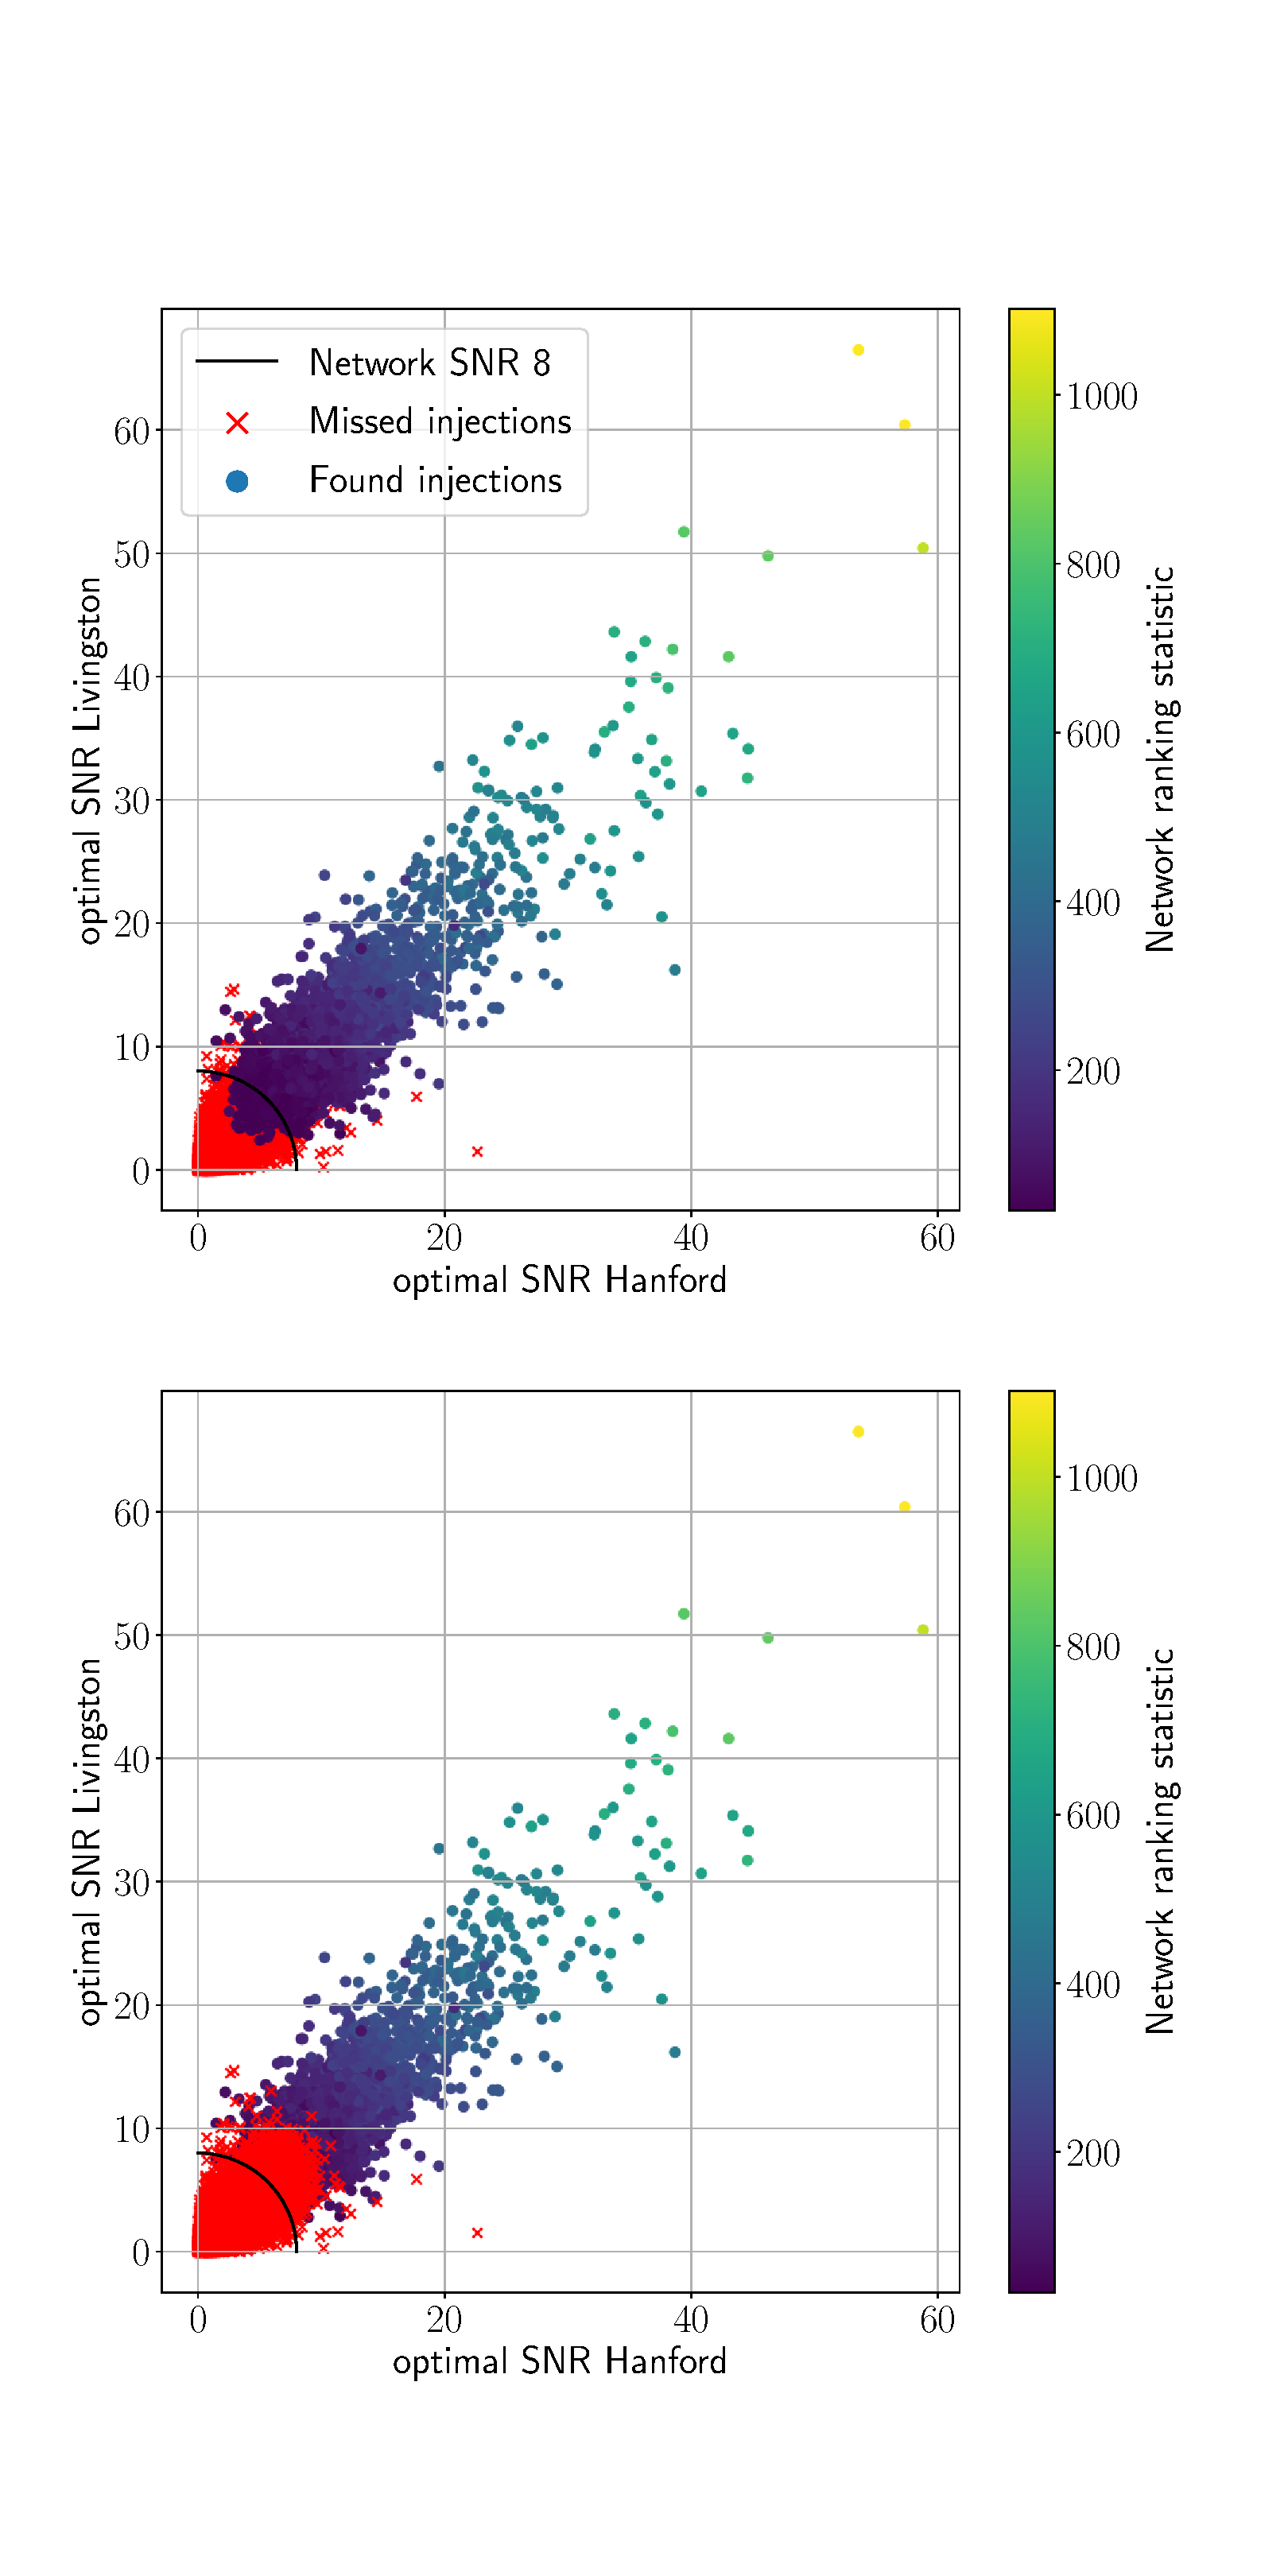
\includegraphics[width=0.6\textwidth, trim=1cm 3.5cm 2cm 6cm, clip]{chapters/cnn_coinc/images/snr-rank-plot.pdf}
    \caption[Found and missed injections]{Found and missed injections from the test set as returned by the procedure discussed in \autoref{sec:cnn_coinc_methods}. The top panel overlays the missed injections by the found injections and the bottom panel reverses the order. The x- and y-axis show the optimal \acrshort{snr}s of the injections in the Hanford and Livingston detector, respectively. The color of found injections represents the combined ranking statistic as defined by equation \eqref{eq:combined_ranking_ml}. Missed injections are marked by a red cross. The black line indicates an optimal network \acrshort{snr} of $8$. The plot is generated at a \acrshort{far} of $1$ false alarm per month.}
    \label{fig:found_missed}
\end{figure}

In \autoref{fig:cnn_coinc_sens} we show the sensitive distance of different algorithms as a function of the \acrshort{far}. The orange lines show the sensitivity curves of the machine learning based algorithms whereas the purple lines show the sensitivities of a comparable matched filter search. The dashed lines show the sensitivity of the searches when only a single detector is considered. We compare those to a two-detector search where we require coincident detections in both detectors. The filled orange line and the dash-dotted purple line show the comparison between the machine learning and matched filter algorithms, respectively, when both impose the same coincidence condition. The filled purple line shows a more realistic application of matched filtering where the consistency of the time of arrival, the phase, the amplitude, as well as the parameters of the best matching template are required.

We find a significant improvement of up to $20\%$ at a given \acrshort{far} when the machine learning algorithm has access to data from both detectors compared to using only data from a single detector. Furthermore, we can probe \acrshort{far}s down to $\approx 4\times 10^{-4}$ false alarms per month without needing to increase the amount of evaluated data by applying time shifts between detectors as described in \autoref{sec:methods:background}. In principle this limit may be decreased even further and time shifts are only limited by the time-of-flight difference between the detectors. The large increase in the available background potentially greatly increases the statistical significance of any event.

The sensitivities of the machine learning search algorithms are compared to an equivalent matched filter search. For the single detector searches given by the dashed lines in \autoref{fig:cnn_coinc_sens} we find that the machine learning algorithm retains at least $91.5\%$ of the sensitivity at a fixed \acrshort{far} of the matched filter analogue. This corresponds to a maximum absolute separation of \SI{200}{\mega\parsec}. This difference in sensitivity is basically unchanged when data from two detectors is considered and both the machine learning as well as the matched filter search calculate coincidences only based on the timing in the different detectors. The corresponding curves in \autoref{fig:cnn_coinc_sens} are the filled orange and the dash-dotted purple line, respectively. In this case, the machine learning algorithm retains at least $92.4\%$ of the sensitivity of the time coincidence matched filter search which corresponds to an absolute separation of \SI{180}{\mega\parsec}.

However, matched filtering also carries information about the intrinsic parameters of the source, the relative phase, and the relative amplitudes in the two detectors. This information can be used to further constrain coincidences and improve the ranking statistic \cite{Nitz:2017svb} by testing for signal consistency. We compare the time coincidence machine learning search (filled, orange line in \autoref{fig:cnn_coinc_sens}) to this matched filter coincidence search utilizing signal consistency checks (filled, purple line in \autoref{fig:cnn_coinc_sens}). The machine learning search now only retains at least $83.9\%$ of the sensitivity in \acrshort{far} regions where both are defined. This corresponds to an absolute separation of \SI{430}{\mega\parsec}.

We truncate the sensitivity curve of any search that has access to data from both detectors in \autoref{fig:cnn_coinc_sens} at a \acrshort{far} of $10^3$ false alarms per month. This is done due to a large number of true positives at high \acrshort{far}s originating from random noise coincidences. This means that the search returns a coincident event that is caused by a particular noise realization which happens to coincide with an injection with an optimal \acrshort{snr} below the trigger threshold. Many of these injections should thus not be recoverable but are detected at high \acrshort{far} due to these noise fluctuations. At a \acrshort{far} of $10^3$ per month we expect less then $\mathcal{O}(10)$ of these false associations. Another reason to only compare the sensitivity at low \acrshort{far}s of the machine learning and the matched filtering based searches are the thresholds used to find triggers. The matched filter search uses a threshold of \acrshort{snr} $5$ whereas the machine learning search uses a threshold on the \acrshort{usr} ranking statistic of $-2.2$. Because there is no direct relation between these two statistics, we cannot guarantee that both thresholds correspond to similar signal strengths. It may be possible that one search excludes weak signals which are found by the other based on this difference in the threshold.

The sensitivity difference between machine learning and matched filtering stays constant between using data from a single detector and using data from two detectors when matched filtering may only check for time consistency between detection candidates from the two observatories. The performance difference increases when matched filtering also checks for signal consistency. It is, therefore, reasonable to believe that a multi detector machine learning search may be more sensitive when it too can check for signal consistency. This would either require the single detector network to output parameter estimates of the detected signal alongside a ranking statistic or a single network that uses the data from both detectors as input. In the following \autoref{sec:two-det-net} we explore the second hypothesis.

\begin{figure}
    \centering
    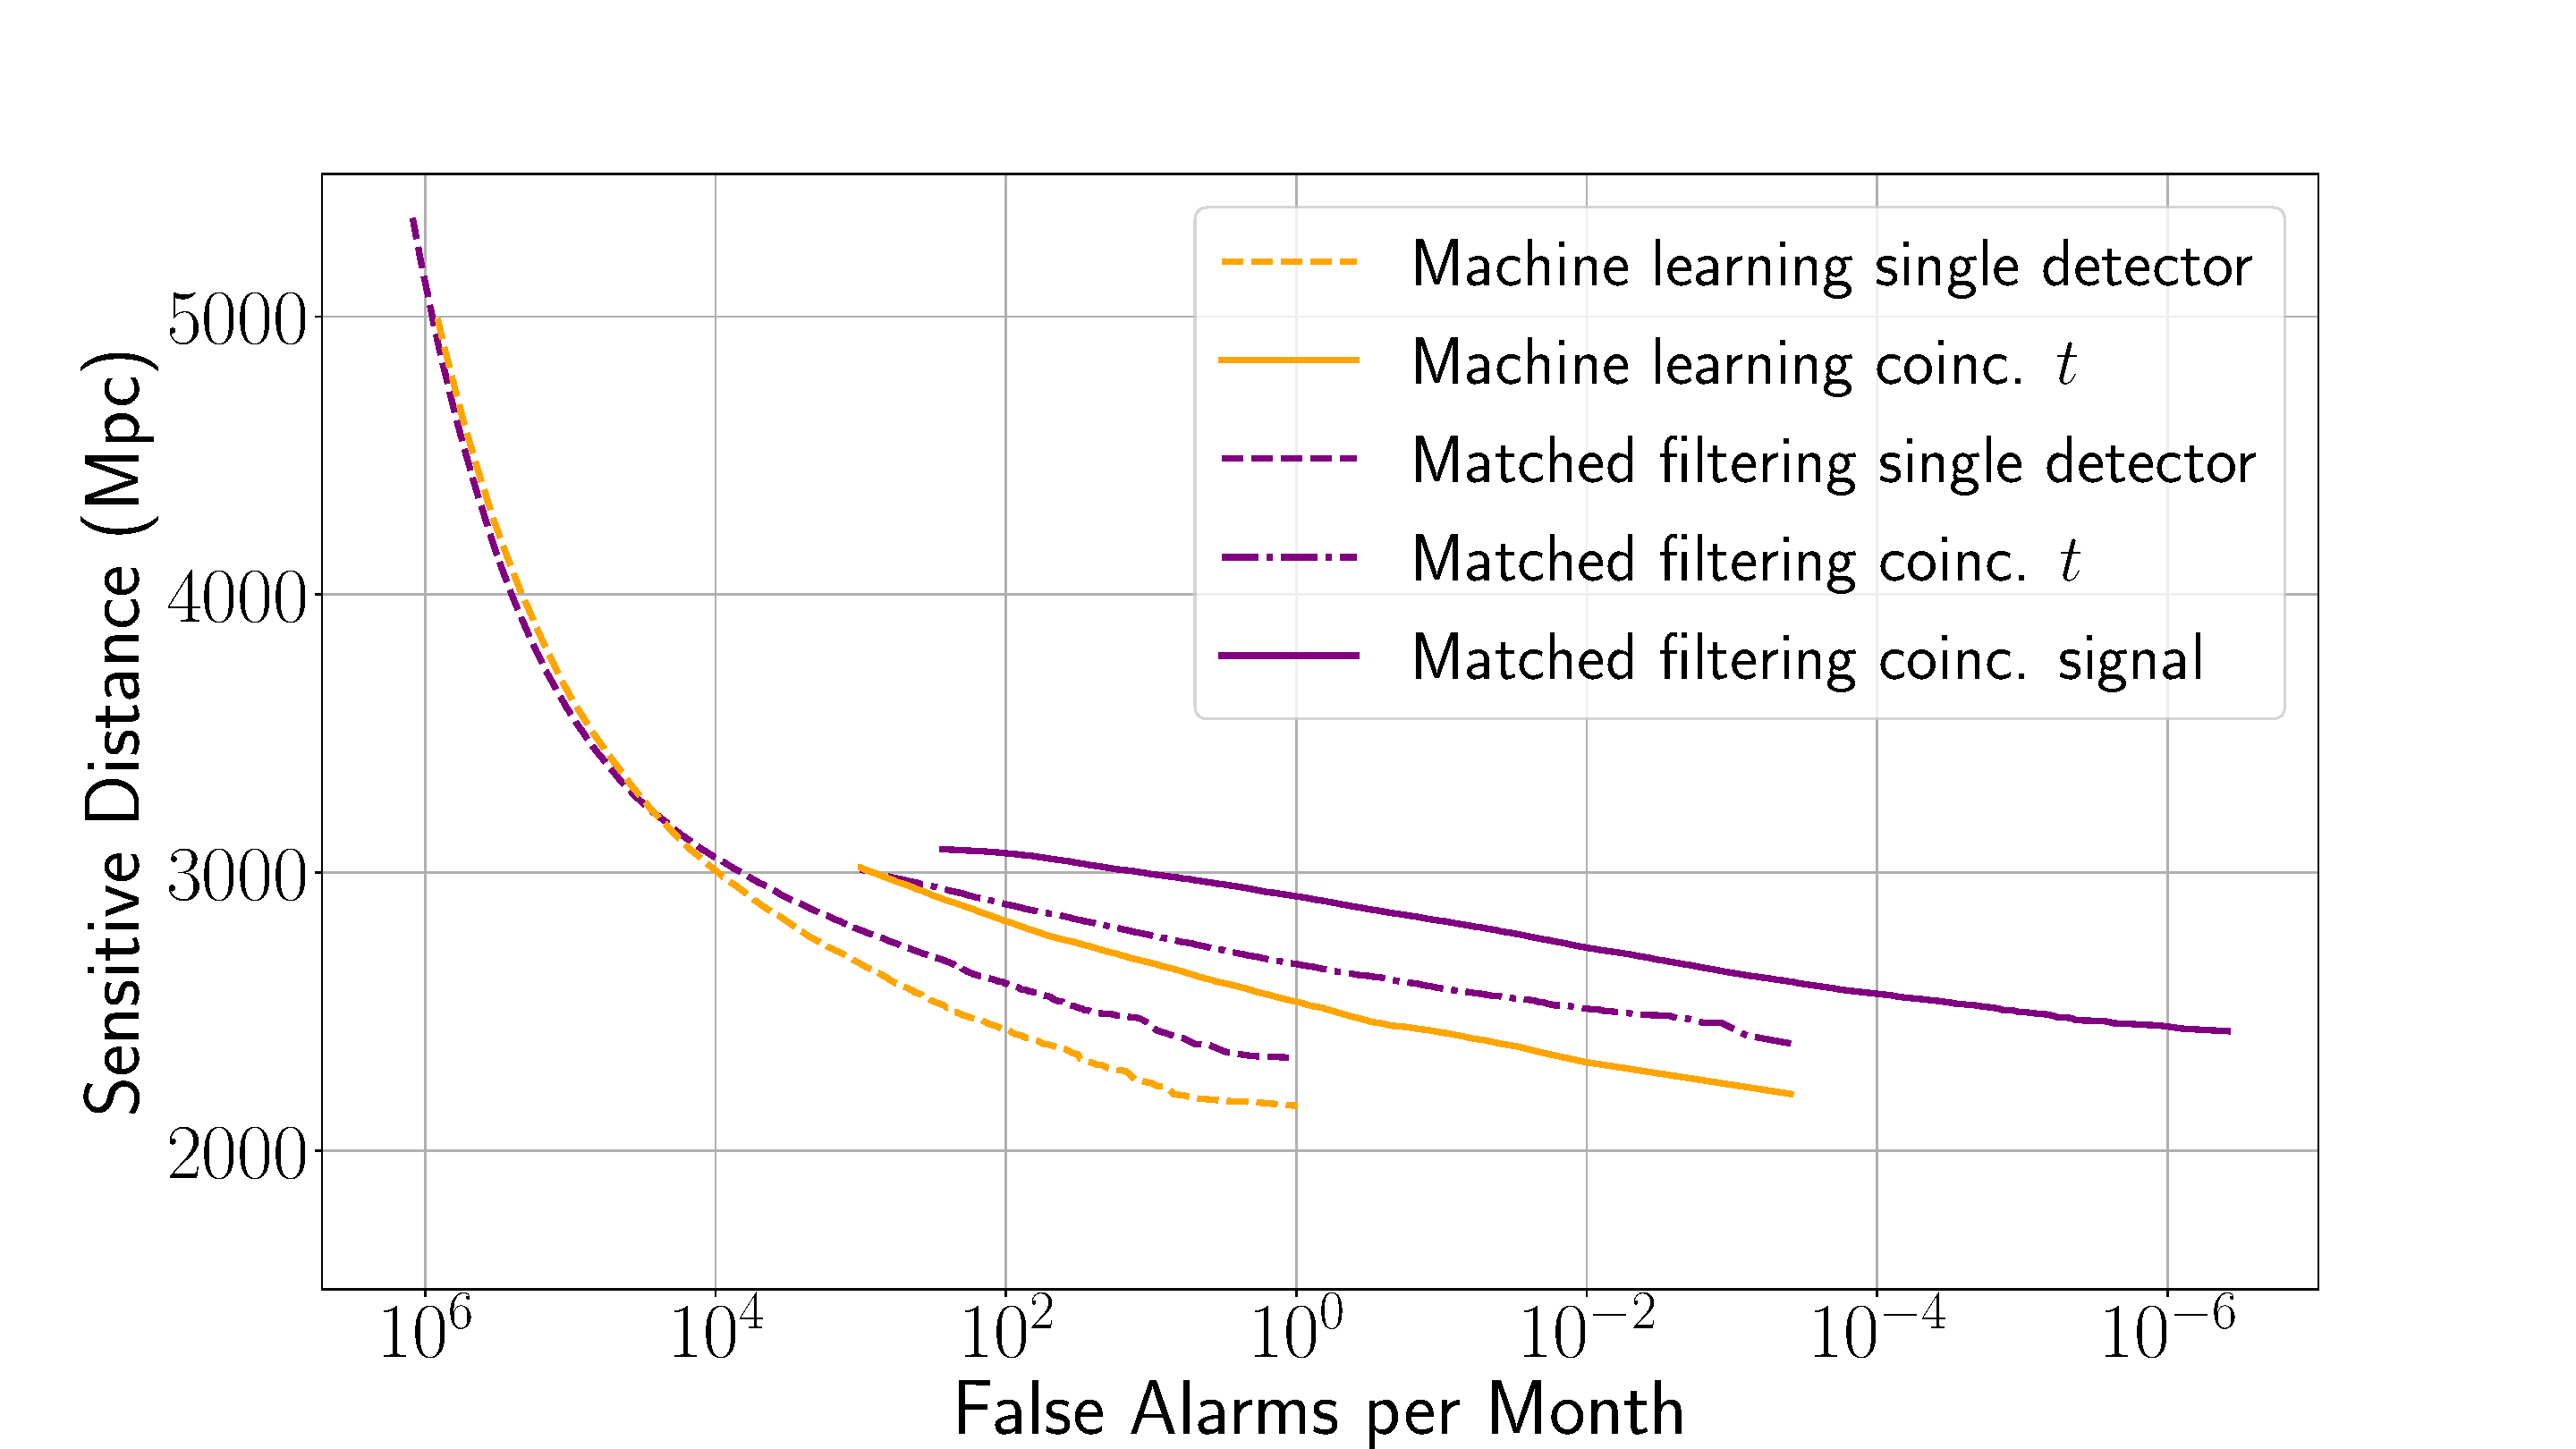
\includegraphics[width=0.8\textwidth, trim=1cm 0 4.2cm 2.5cm, clip]{chapters/cnn_coinc/images/sens.pdf}
    \caption[Sensitive distances as function of false-alarm rate of coincidence searches]{Shown are the sensitive distances of different search algorithms as a function of the \acrshort{far}. In orange we show the sensitivity curves of the machine learning based searches presented in \cite{Schafer:2021fea} and this work. In purple we show sensitivity curves of an equivalent matched filter search. The dashed lines are derived on data only from a single detector. A label ''coinc. $t$'' refers to events being tested for coincidence based solely on the time difference of the events in the two detectors. The label ''coinc. signal'' means that the matched filter search also checked for signal consistency based on the time-, phase-, amplitude-difference, and intrinsic parameters in the two detectors. Sensitivities derived on data from more than one detector are truncated at a \acrshort{far} of $10^3$ per month due to an increasing number of true detections caused by random coincident events in the noise.}
    \label{fig:cnn_coinc_sens}
\end{figure}


\section{Two Detector Network}\label{sec:two-det-net}
The deep learning algorithm presented in \autoref{sec:cnn_coinc_methods} is significantly less sensitive than the full matched filter analysis that takes signal consistency into account. On the other hand, when the deep learning algorithm is compared to the matched filter search where signal consistency is ignored, the difference in sensitivity is comparable to the difference in sensitivity for a single detector. This gives reason to believe that the difference in sensitivity compared to the full matched filter search could be reduced when the network may operate on the data from both detectors and consider coincidences itself.

\subsection{Architecture}
We construct a network that uses data from both detectors while still retaining the ability to efficiently estimate a large background. The network from \autoref{sec:cnn_coinc_methods} is still applied to the data from the two detectors individually. However, the final layer is removed and the $64$ output-neurons from both networks are concatenated. We then add $3$ more fully connected layers to look for coincidences between the detectors. An overview of the network is shown in \autoref{fig:2det-net}.

\begin{figure}
    \centering
    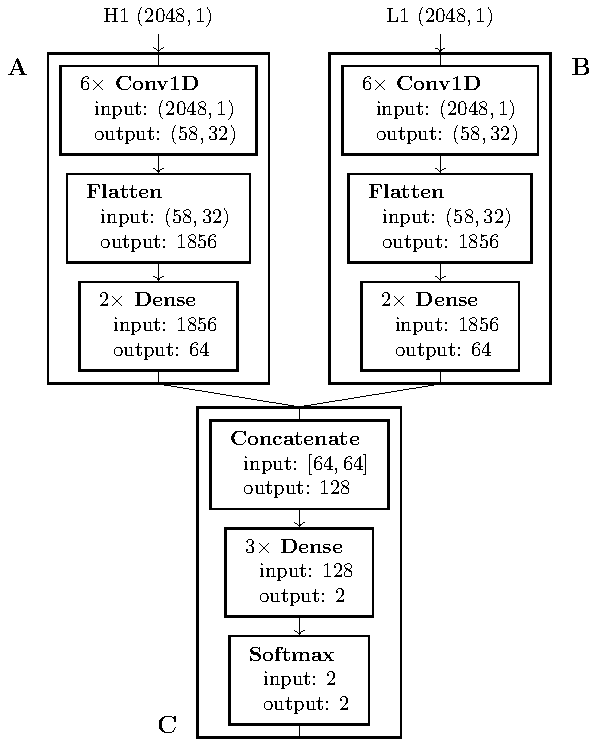
\includegraphics[width=0.7\textwidth]{chapters/cnn_coinc/images/2det-net.pdf}
    \caption[Coincidence network architecture]{A high level overview of the two-detector architecture. The network consists of three sub-networks A, B, and C. A detailed description of the sub-networks A and B can be found in \autoref{tab:cnn_coinc_network} by removing the final row. The fully connected Dense layers contain $128$, $64$, and $2$ neurons in that order. All but the final Dense layer are equipped with an exponential linear unit (ELU) activation.}
    \label{fig:2det-net}
\end{figure}

The last layer from the single detector network is removed to create a large latent space. A matched filter search compresses the input data into the ranking statistic, the time of the merger, and the parameters of the best matching template. The intention is that $64$ neurons may be sufficient for a comparable compression and that the additional layers that operate on the concatenated outputs could perform a signal consistency analysis.

The sub-networks A and B in \autoref{fig:2det-net} are intended to act as encoders that reduce the $2048$ dimensional input into a latent space of dimension $64$. It may be interesting in the future to train these sub-networks initially as autoencoders \cite{Kramer:1991aaa} from which only the encoder is used for detection purposes afterwards. Autoencoders are neural networks which in the most simple form consist of an encoder network and a decoder network. The encoder network compresses the input to some lower dimensional latent representation whereas the decoder uses that lower dimensional representation to reconstruct the input. Other studies have already found that autoencoders have potential applications in \acrshort{gw} data analysis \cite{Shen:2019ohi, Gabbard:2019rde}.

\subsection{Data Sets and Training}
The network is trained on data similar to that presented in \autoref{sec:training:data}. However, the data is extended to two detectors and sources are uniformly distributed in the sky. The latter change is required due to the amplitude and phase correlations in the two detectors. We use the same number of noise and signal samples as in \autoref{sec:training:data}.

We utilize the pre-trained single detector network used in \autoref{sec:cnn_coinc_methods} in two different ways. In both cases the single detector parts of the two detector network (A and B in \autoref{fig:2det-net}) are initialized with the weights of the pre-trained model from \autoref{sec:cnn_coinc_methods}. However, for one of the two networks, these weights are then not optimized during training, leaving only the weights of the final fully connected layers (C in \autoref{fig:2det-net}) to be adjusted. This approach is known as transfer learning \cite{Weiss:2016aaa} and has been successfully applied for different problems \cite{Tan:2018aaa, George:2018awu, Mesuga:2021qeq}. The second network optimizes the weights of the entire network. We also train a third network of the same architecture, where all parameters are initialized randomly and optimized during training.

The same optimizer settings and loss function described in \autoref{sec:training:data} are used to train all three networks for $300$ epochs. They are trained with a Softmax activation on the final layer, which is removed during evaluation. Each network is only trained once and the epoch with the highest efficiency on the validation set is chosen for further analysis.

\subsection{Coincident Events}
Because the networks output a single value when given the data from two detectors, we interpret that output as a coincidence ranking statistic at the corresponding time. We then perform the same clustering and thresholding described in \autoref{sec:methods:single_det} to obtain a list of coincident events.

\subsection{Background Estimation}
Determining the background of the two detector network is more challenging than for the single detector network from \autoref{sec:methods:background}, as there is no direct way of performing time shift in a computationally efficient way. One would, therefore, naively be limited by the duration of the analyzed data or would have to re-evaluate the entire month of test data multiple times. However, the network is designed in such a way that the data from both detectors are still analyzed individually and combined only at later stages. We evaluate the single detector data individually with the sub-networks A and B from \autoref{fig:2det-net} and store those outputs. We then permute the order of the outputs from sub-network B such that it corresponds to a time shift with respect to the output from sub-network A. Finally, sub-network C is applied to the concatenated data from sub-network A and B for many different time shifts. Since sub-network C is very simple and time shifts can be generated trivially this process generates $\mathcal{O}\left(1000\right)$ months of background within $<$ \SI{12}{\hour} on a NVIDIA RTX 2070 Super.

\subsection{Evaluation and Comparison to Matched Filtering}
\autoref{fig:dual_net_sens} shows the sensitive distance of the various networks as a function of the \acrshort{far} and compares them to the results presented in \autoref{sec:net_sens}. All curves are truncated at a \acrshort{far} of $10^3$ per month due to the large number of false associations described in \autoref{sec:net_sens}. The three networks utilizing the data from both detectors described in this section are labeled as ''Machine learning network coinc.''. The matched filter results are shown in purple, where the dash-dotted line considers only time coincidence and the filled line also takes the consistency of intrinsic source parameters, phase, and amplitude into account. The orange line corresponds to the network from \autoref{sec:cnn_coinc_methods}.

\begin{figure}
    \centering
    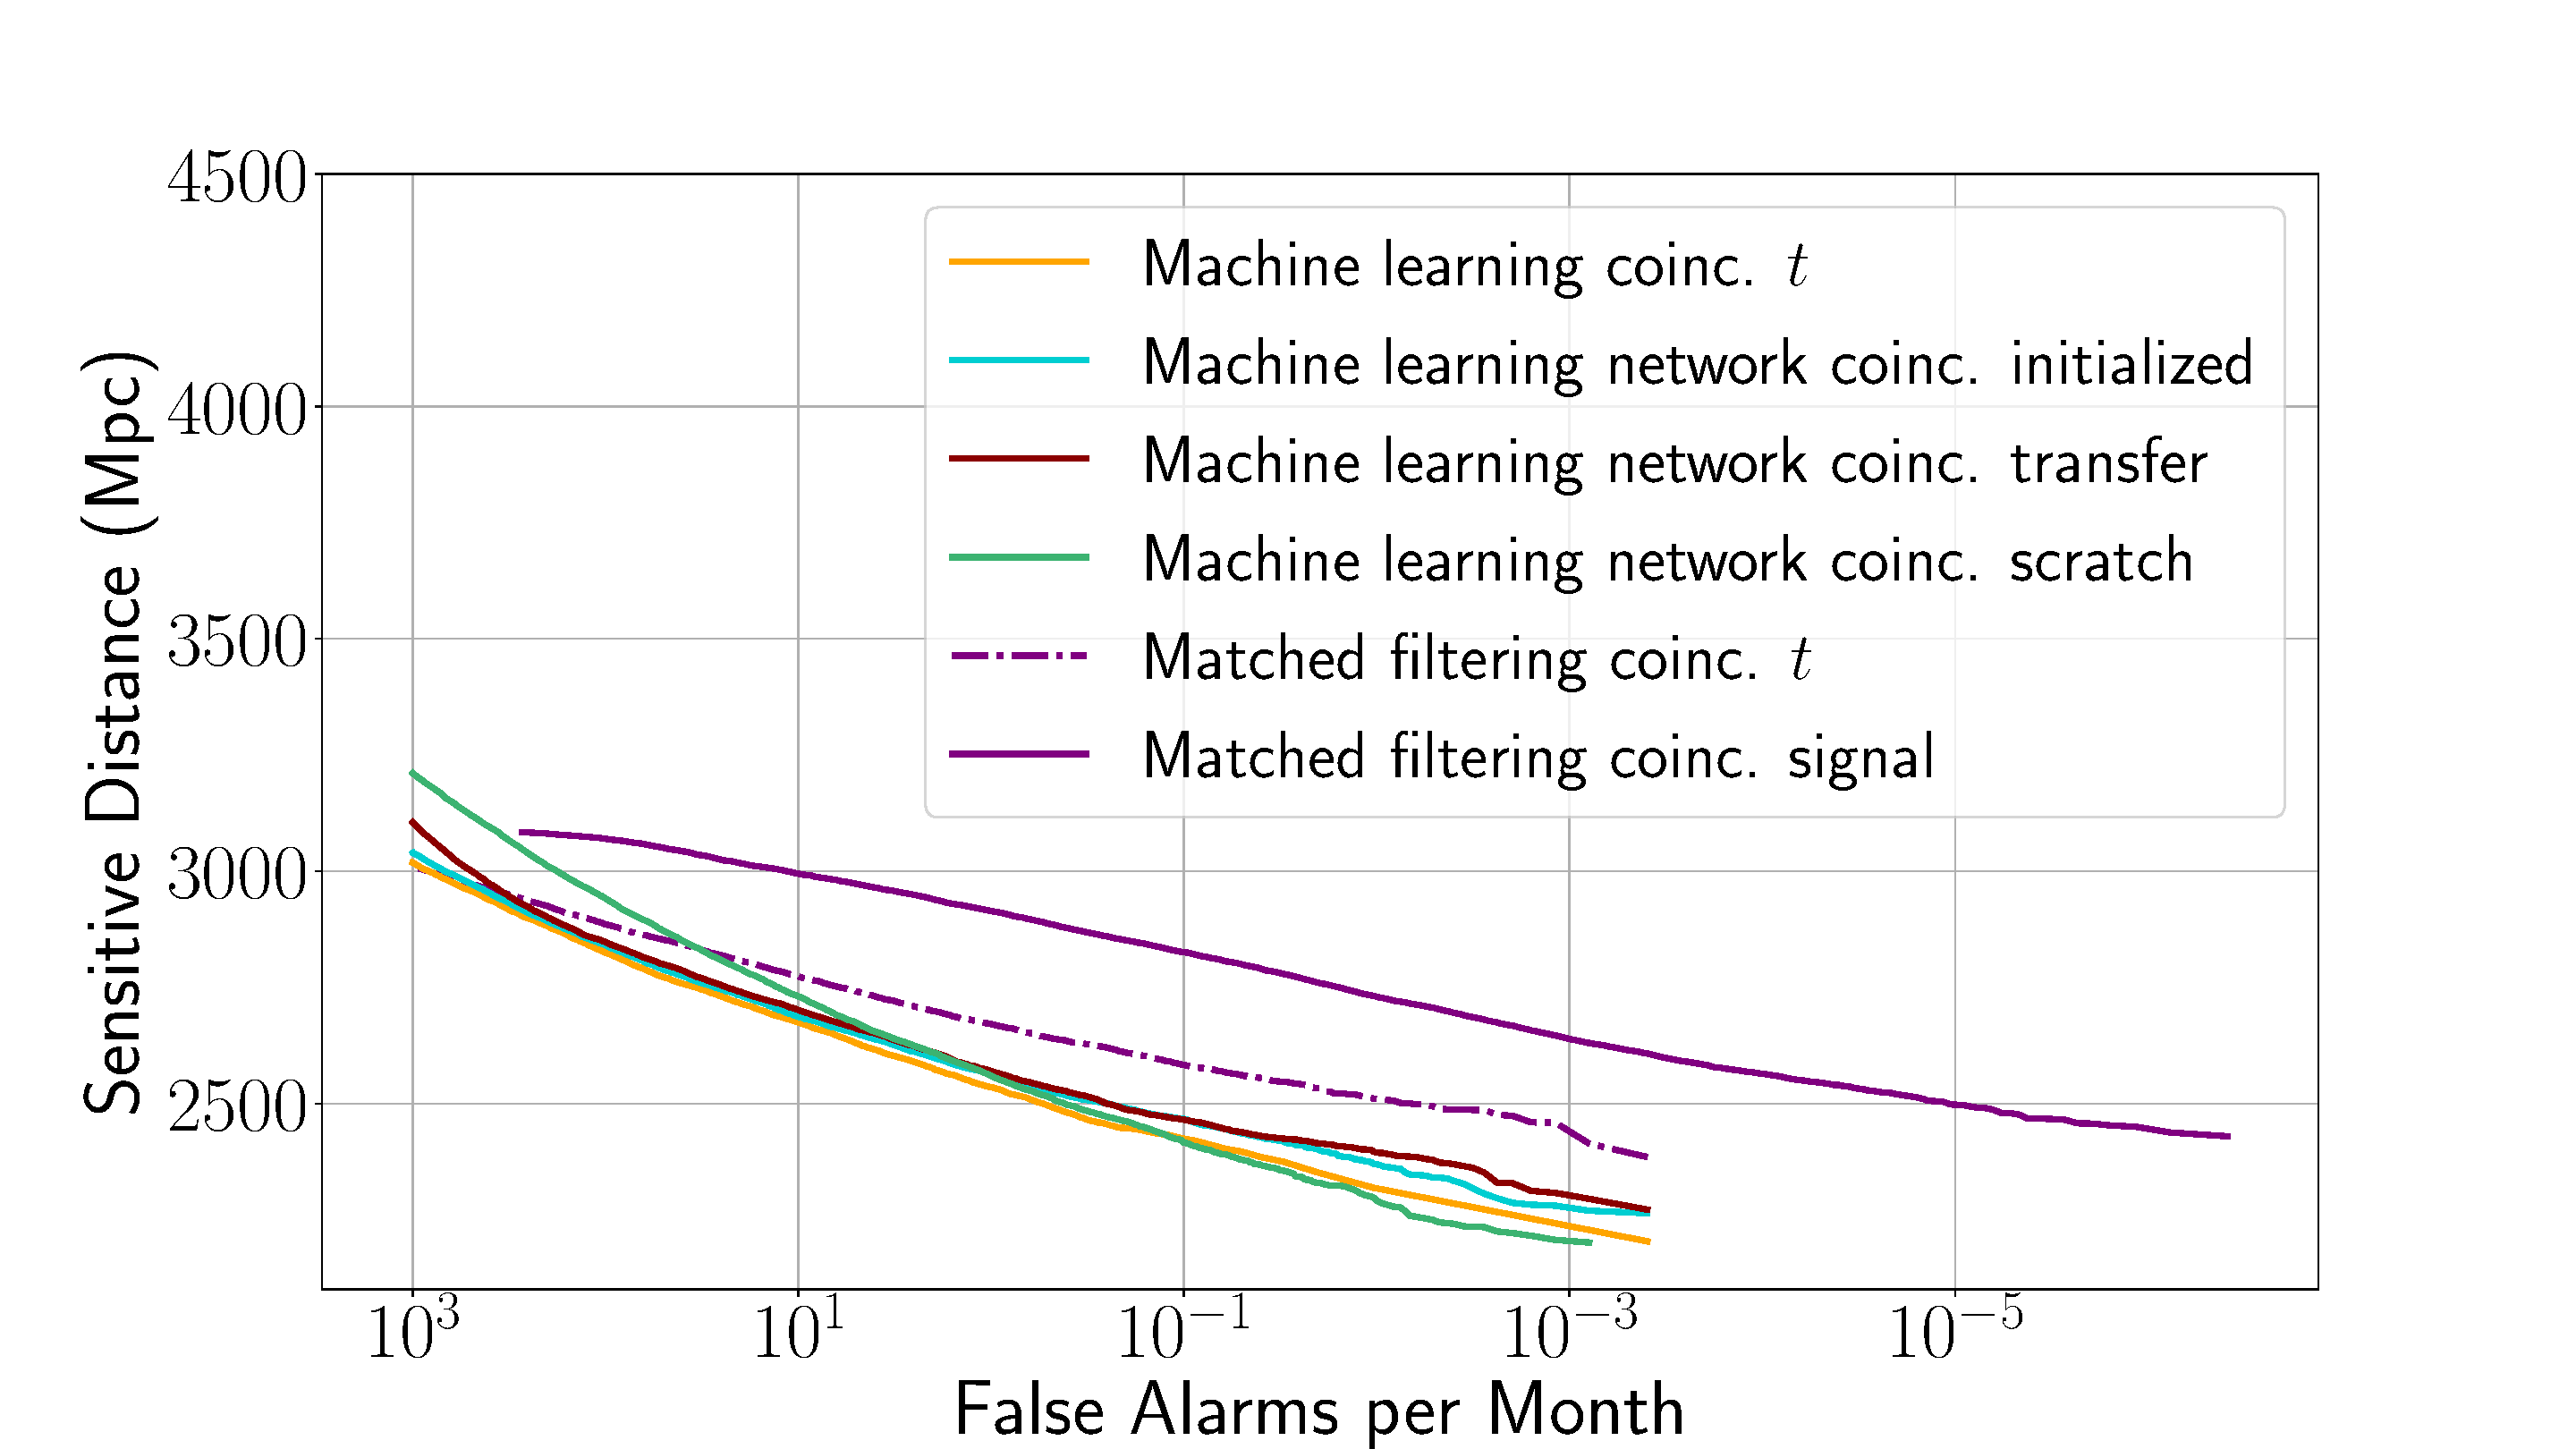
\includegraphics[width=0.8\textwidth, trim=1cm 0 4cm 3cm, clip]{chapters/cnn_coinc/images/sens-2.pdf}
    \caption[Sensitivity of different coincidence strategies]{The sensitivity of different search algorithms as a function of the \acrshort{far}. All shown algorithms operate on the data from two detectors. The curves labeled ''Machine learning coinc.'' are neural network search algorithms that consider data from both detectors and an overview can be found in \autoref{fig:2det-net}. The network labeled ''initialized'' initializes the sub-networks A and B as shown in \autoref{fig:2det-net} from the single detector network used in \autoref{sec:net_sens} but optimizes them during the subsequent training. The network labeled ''transfer'' also initializes both sub-networks as the ''initialized'' network but freezes their weights. The network labeled ''scratch'' initializes all parameters of the network randomly. All other searches operate on the data from the individual detectors first and then search for coincident events. A label ''coinc. $t$'' refers to events being tested for coincidence based solely on the time difference of the events in the two detectors. The label ''coinc. signal'' means that the matched filter search also checked for signal consistency based on intrinsic parameters and the time-, phase-, and amplitude-difference in the two detectors. The curve labeled ''Machine learning coinc. $t$'' refers to the two-detector machine learning search analyzed in \autoref{sec:net_sens}. All sensitivities are truncated at a \acrshort{far} of $10^3$ per month due to a growing number of true positive detections caused by the coincidence of noise events.}
    \label{fig:dual_net_sens}
\end{figure}

The networks described in this section were designed to be able to take signal consistency into account by reducing the input data to a large latent space. As such we were expecting sensitivities at low \acrshort{far}s to be larger than those obtained from time coincidence between single detector events produced by the single detector network.

However, we find that at low \acrshort{far}s all of the two detector networks are roughly as sensitive as the network tested in \autoref{sec:net_sens}. Therefore, they are still less sensitive than the matched filter equivalent and do not seem to take signal consistency into account. For high \acrshort{far}s, on the other hand, they are more sensitive. We suspect that the large time variation of the peak amplitude of \SI[parse-numbers=false]{\pm 0.1}{\second} may be responsible for this behavior. The networks are, thereby, trained to be insensitive to variations in timing of less then \SI{0.1}{\second}, which may produce phase and amplitude variations in a broad range.

\section{Conclusions}\label{sec:cnn_coinc_conclusions}
In this paper we have extended the single detector deep learning \acrshort{gw} search algorithm from \cite{Gabbard:2017lja, Schafer:2021fea} to two detectors and compared it to an equivalent matched filter algorithm. We found that the most simple extension, applying the one detector network to the data from two detectors individually and searching for coincident events, retains $\approx 92\%$ of the sensitivity of matched filtering, when only the time consistency between detectors is required. This fraction drops to $\approx 84\%$ when signal consistency between detectors is also considered.

To operate on data from two observatories, we constructed a two detector ranking statistic for the machine learning search based on the single detector \acrshort{usr} ranking statistic proposed in \cite{Schafer:2021fea}. This ranking statistic proved to be correlated with the network \acrshort{snr}.

We also highlighted the advantages of using a single detector network to construct a two detector search. First, the single detector network does not need to be re-trained to be applied to the second detector, if both have similar noise characteristics. Second, this approach enables an efficient background estimation by applying relative time shifts to the recovered single detector events. This allows to test the two detector search to almost arbitrarily low \acrshort{far}s at low computational expenses. This method has already proven to be effective and reliable in state-of-the-art classical search algorithms \cite{LIGOScientific:2020ibl, Usman:2015kfa, Sachdev:2019vvd}.

Because using a single detector network restricts one to check for coincidences based solely on the timing difference, we tested a simple network that operates on data from both detectors directly. This allows the network in principle to construct internal signal representations which can be correlated between observatories. The network was constructed by removing the final layer of the single detector network, concatenating the outputs and adding a few fully connected layers to check for coincident events. The final fully connected layers, thus, receive $64$ latent variables for each detector that can be checked for coincidence.

This design of the two detector network allowed us to do efficient background estimation. By applying relative time shifts to the outputs of the individual detector sub-networks, only the final few fully connected layers need to be evaluated for all shifts. The bulk of the computation, namely evaluating the input data of the detectors, only needs to be done once.

The network architecture was trained in three different ways; randomly initialized parameters for the entire network, parameters of the sub-networks initialized from the single detector network, and parameters of the individual detector sub-networks fixed to the single detector parameters and optimizing only the final fully connected layers.

We found that all of these networks have very similar performance at low \acrshort{far}s. Neither of them performed substantially better than the initial network that looked for time coincident events between the single detector network outputs. It, therefore, seems as if the network architecture explored here is unable to learn any additional information about the signal. This may be caused by the allowed time-variance of \SI[parse-numbers=false]{\pm 0.1}{\second} for signals in the training set, which may limit the time resolution of the network and thus overshadow correlations in any other parameters. More sophisticated network architectures with higher time resolution may improve our findings. First promising steps have already been taken by \cite{Wei:2020ztw, Huerta:2020xyq}. Using an autoencoder to find a more meaningful latent representation of the input data may also be of use.

While the sensitivity was not improved by using a single network to process the data of two detectors, we still want to highlight that the method of determining the background may be of use for future networks.

Here we limited our research to \acrshort{gw}s from non-spinning binary black holes with signal duration $<$ \SI{1}{\second} and Gaussian noise. Any of these simplifications are desirable to be lifted. Especially considering real noise may increase the gap in sensitivity between the single detector and multi detector search algorithm, by vetoing glitches. While we considered only two detectors an extension to a larger network should be trivial and may follow studies such as \cite{Davies:2020tsx}.

\chapter{MLGWSC-1: The first Machine Learning Gravitational-Wave Search Mock Data Challenge}\label{ch:mlgwsc1}
\minitoc
This chapter is essentially a full reprint of \cite{Schafer:2022dxv} with some minor edits for formatting and adjustments to address comments from two referee reports. It discusses the results of a mock data challenge we organized that was targeted at placing machine learning \acrshort{gw} searches into the context of existing, state-of-the-art algorithms.

\setcounter{section}{-1}
\section{Abstract}
We present the results of the first Machine Learning Gravitational-Wave Search Mock Data Challenge (\acrshort{mlgwsc1}). For this challenge, participating groups had to identify gravitational-wave signals from binary black hole mergers of increasing complexity and duration embedded in progressively more realistic noise. The final of the 4 provided datasets contained real noise from the O3a observing run and signals up to a duration of 20 seconds with the inclusion of precession effects and higher order modes. We present the average sensitivity distance and runtime for the 6 entered algorithms derived from 1 month of test data unknown to the participants prior to submission. Of these, 4 are machine learning algorithms. We find that the best machine learning based algorithms are able to achieve up to $95\%$ of the sensitive distance of matched-filtering based production analyses for simulated Gaussian noise at a false-alarm rate (\acrshort{far}) of one per month. In contrast, for real noise, the leading machine learning search achieved $70\%$. For higher \acrshort{far}s the differences in sensitive distance shrink to the point where select machine learning submissions outperform traditional search algorithms at \acrshort{far}s $\geq 200$ per month on some datasets. Our results show that current machine learning search algorithms may already be sensitive enough in limited parameter regions to be useful for some production settings. To improve the state-of-the-art, machine learning algorithms need to reduce the false-alarm rates at which they are capable of detecting signals and extend their validity to regions of parameter space where modeled searches are computationally expensive to run. Based on our findings we compile a list of research areas that we believe are the most important to elevate machine learning searches to an invaluable tool in gravitational-wave signal detection.

\section{Introduction}
The first gravitational-wave (\acrshort{gw}) observation on September 14, 2015~\cite{LIGOScientific:2016aoc} achieved by the LIGO and Virgo Collaboration~\cite{LIGOScientific:2014pky, VIRGO:2014yos} started the era of \acrshort{gw} astronomy. During the first observing run (\acrshort{o1}) two more \acrshort{gw}s from coalescing binary black holes (\acrshort{bbh}s) were detected. The second observing run (\acrshort{o2}) saw $\mathcal{O}(10)$ additional confident \acrshort{bbh} detections as well as the first detection of a binary neutron star (\acrshort{bns}) merger~\cite{LIGOScientific:2017vwq, LIGOScientific:2018mvr, Nitz:2018imz, Nitz:2020oeq, Venumadhav:2019tad, Venumadhav:2019lyq}. The third observing run (\acrshort{o3}) was split into two parts, \acrshort{o3a} and \acrshort{o3b}. During \acrshort{o3a} a further $\mathcal{O}(40)$ \acrshort{bbh}s as well as a second \acrshort{bns} merger were reported~\cite{LIGOScientific:2020ibl, LIGOScientific:2021usb, Nitz:2021uxj}. \acrshort{o3b} added another $\mathcal{O}(40)$ \acrshort{bbh} events as well as finding the first two confident detections where the component masses are consistent with the merger of a neutron star black hole system (\acrshort{nsbh})~\cite{LIGOScientific:2021djp, Nitz:2021zwj}. The fourth observing run (\acrshort{o4}) is scheduled to begin in early 2023 and is expected to significantly increase the volume from which sources can be detected~\cite{KAGRA:2013rdx, Cahillane:2022pqm}.

\acrshort{gw} signals are commonly identified in the background noise of the detectors using matched filtering~\cite{LIGOScientific:2021djp, Messick:2016aqy, DalCanton:2020vpm, Adams:2015ulm}. Matched filtering compares pre-computed models of expected signals, known as templates, with the data from the detectors~\cite{Allen:2005fk}. When a model matches the data to a pre-defined degree and data-quality requirements are met, a candidate detection is reported.
Loosely modelled searches~\cite{Klimenko:2005xv, Klimenko:2015ypf, Lynch:2015yin}, which look for coherent excess power in multiple detectors, are also employed by the LIGO-Virgo-KAGRA collaboration (\acrshort{lvk}) to find potential signals.

The rate of detections has drastically increased from \acrshort{o1} to \acrshort{o3}. This increase was enabled by continued detector upgrades at the two advanced LIGO observatories in Hanford and Livingston~\cite{LIGOScientific:2014pky}, as well as sensitivity improvements for the advanced Virgo detector~\cite{VIRGO:2014yos}. With the entry into service of Kagra~\cite{KAGRA:2018plz} a fourth observatory joined the network of ground based \acrshort{gw}-detectors towards the end of \acrshort{o3}. The rate of detections is expected to further increase during \acrshort{o4} as the sensitivity of the detectors improves and the volume from which sources can be detected grows.

With an increasing rate of detections, it is likely that systems with unexpected physical properties will be observed more frequently in the future. Optimally searching for these is a challenge for matched filtering based searches, where the computational cost scales linearly with the number of templates used. The inclusion of effects such as precession, eccentricity, or higher order modes requires millions of templates to not miss potential signals~\cite{Harry:2016ijz, Harry:2017weg, Dhurkunde:2022aek} and thus are computationally prohibitive, especially when real-time alerts should be issued. Loosely modeled searches are inherently capable of detecting arbitrary sources at a fixed computational cost but are prone to miss more signals due to their lower sensitivity in parameter regions where accurate models exist.

In recent years, machine learning has been applied in many scientific fields to enable or improve research into computationally expensive topics~\cite{Deiana:2021niw}. Some examples include the prediction of protein structure used in pharmaceutical studies~\cite{Alquraishi:2021aaa}, improvements to material composition and synthesis~\cite{Butler:2018aaa}, or event reconstruction at the Large Hadron Collider~\cite{Gray:2020mcm}. There is also ongoing research into using neural networks to discover closed form expressions from raw data~\cite{Cranmer:2020wew} or optimizing machine learning algorithms to take advantage of physical symmetries of the underlying problem~\cite{Smidt:2020tuy, Oxley:2021aaa, Dax:2021myb}.

More relevant to this work, machine learning algorithms have also started to be explored as alternative algorithms for many \acrshort{gw} data-analysis tasks. These include detector glitch classification~\cite{Zevin:2016qwy, George:2017fbn, Bahaadini:2018git}, parameter estimation~\cite{Chua:2019wwt, Gabbard:2019rde, Chatterjee:2019avs, Dax:2021tsq, McLeod:2022ccr}, continuous \acrshort{gw} detection~\cite{Dreissigacker:2019edy, Morawski:2019awi, Miller:2019jtp, Dreissigacker:2020xfr, Beheshtipour:2020zhb, Beheshtipour:2020nko, Yamamoto:2022adl}, enhancements for existing pipelines~\cite{Chatterjee:2019gqr, Cabero:2020eik, Jadhav:2020oyt, Williams:2021qyt, Mishra:2021tmu, Lopez:2021ikt, Mishra:2022ott, McIsaac:2022odb}, surrogate waveform models~\cite{Khan:2020fso, Nousi:2021arn, Fragkouli:2022lpt}, as well as various signal detection algorithms~\cite{George:2016hay, George:2017pmj, Gabbard:2017lja, Gebhard:2019ldz, Krastev:2019koe, Krastev:2020skk, Wei:2020ztw, Schafer:2020kor, Wei:2020sfz, Wei:2020xrl, Huerta:2020xyq, Skliris:2020qax, Morawski:2021kxv, Schafer:2021fea, Schafer:2021cml, Khan:2021vbf, Ruan:2021fxq, Chaturvedi:2022suc, Baltus:2022pep, Moreno:2021fvp, Bacon:2022lsm}. For a summary of many methods we refer the reader to \cite{Cuoco:2020ogp, Huerta:2021ybd}. In this work we focus solely on detection algorithms for \acrshort{bbh} \acrshort{gw} signals, which have been the most commonly observed type of sources to date~\cite{LIGOScientific:2020ibl, LIGOScientific:2021usb, Nitz:2021uxj}. These signals are the easiest to detect for machine learning algorithms due to their short duration.

Many of the works considering the usage of machine learning for \acrshort{gw} signal detection are difficult to cross-compare. Most algorithms target different datasets and derived metrics are often motivated more by machine learning practices than by state-of-the-art \acrshort{gw} searches. It is, therefore, hard to pinpoint exactly how capable machine learning search algorithms currently are and where the main difficulties arise. To achieve the goal of an objective characterization of machine learning \acrshort{gw} search capabilities, a common ground for comparison is required.

Here we present the results of the first Machine Learning Gravitational-Wave Search Mock Data Challenge (\acrshort{mlgwsc1}). In an attempt to provide a common ground of comparison for different algorithms and in preparation of \acrshort{o4}, we have calculated sensitive distances from 6 different submissions calculated on datasets of one month duration to collect and compare a suite of searches. We want to motivate the utilization of machine learning based searches in a production setting by providing a definitive resource to allow for easy comparison between different algorithms, be it machine learning based, matched filtering based, or completely unmodeled. This challenge is the first of its kind\footnote{There has previously been a public Kaggle challenge \cite{EGO:2021aaa}. First in the sense of this paper refers to our setup of providing continuous data.} and hopefully more will be held in the future, expanding to more difficult scenarios.

The mock data used in this challenge consists of 4 datasets containing noise of increasing realism and signals with increasing complexity for the two detectors LIGO Hanford and LIGO Livingston~\cite{LIGOScientific:2014pky}. The final dataset challenges participants to identify \acrshort{gw}s from spinning \acrshort{bbh}s with a duration of up to \SI{20}{\second} added to real detector noise from \acrshort{o3a}. The signals also take precession effects and higher order modes into account.

Submissions are evaluated on mock data of one month duration for each of the four datasets. We calculate sensitive distances for each algorithm and estimate the computational efficiency based on the runtime. The final dataset should provide an accurate picture of the possible real-world performance these algorithms can achieve. However, we note that direct comparison of the runtime performance of the different algorithms is complicated by differing hardware usage and optimization.

We find that machine learning algorithms are already competitive with state-of-the-art searches on simulated data containing injections drawn from the limited parameter space covered by this challenge. The most sensitive machine learning algorithm manages to retain $\geq 93\%$ of the sensitive distance measured for the \pycbc pipeline~\cite{Nitz:2021zwj} on Gaussian background data down to a false-alarm rate (\acrshort{far}) of $1$ per month. For higher \acrshort{far}s the separation between the approaches generally shrinks.

Most machine learning searches, as tested here, are less sensitive on real noise than on simulated data. The traditional algorithms handle this transition better. As a consequence, the most sensitive machine learning algorithm retains $\geq 70\%$ of the sensitive distance of the \pycbc search down to a \acrshort{far} of 1 per month. However, the sensitivity achieved of machine learning algorithms on real data is still substantial and shows that they are capable of rejecting non-Gaussian noise artifacts without any hand-tuned glitch classification.

From the evaluation of the different datasets we conclude that the main difficulties for current machine learning algorithms are the ability to analyze the consistency of detected signals between detectors and the maximum duration of signals that can be detected. Solving these issues would allow for better performance at \acrshort{far}s $<1$ per month and enable a fast detection of potentially electromagnetic bright sources such as \acrshort{bns} or \acrshort{nsbh} mergers.

All code used in this challenge is open source and available at~\cite{github}. Therein we also collect the individual submissions by groups that have given their consent, provide the analysis results, and make available all plots used in this paper for all submissions.

This paper is structured as follows. In \autoref{sec:mlgwcs_methods} we provide the details on the challenge, the datasets, as well as the evaluation process. All submissions are briefly introduced in \autoref{sec:submissions}. The results of the challenge and a brief discussion can be found in \autoref{sec:results}. We conclude and give an outlook into possible future work in \autoref{sec:mlgwsc_conclusions}.


\section{Methods}\label{sec:mlgwcs_methods}
All submissions described in \autoref{sec:submissions} are evaluated on the same datasets, and all machine learning submissions are evaluated under the same conditions. Below we describe the provided material from the challenge, the requirements for the submitted algorithms, as well as the evaluation process.

\subsection{Challenge Resources}
In this challenge participants are asked to identify \acrshort{gw} signals submerged in detector noise. To provide grounds of comparison, all submissions are evaluated on the same datasets. To allow for optimization of the submitted algorithms for the task at hand, participants had access to code that allowed them to generate arbitrary amounts of data equivalent to that used during the final evaluation of this challenge. All code used for data generation and algorithm evaluation is open source and can be found at~\cite{github}.

In particular, participants had access to the code that was used to generate the final challenge sets, but not the specific seed that was used. The specifics of the datasets are described in \autoref{sec:data}. They were also provided with the code that was used to generate the metrics we provide in this paper. Details on the metrics can be found in \autoref{sec:metrics}.

\subsection{Test Data}\label{sec:data}
The challenge provides a script to generate semi-continuous raw test data for any of the four datasets described below. It allows the user to choose a specific seed and a total duration of the output data. The code subsequently generates up to three files; the first containing pure noise, the second containing the same noise with injected \acrshort{gw} signals, and the third containing the parameters of the injected signals.

The files containing the pure noise and the noise with additive signals are of the same structure. They are HDF5 \cite{hdf5} files with two groups named ``H1'' and ``L1'' containing data from the two detectors LIGO Hanford and LIGO Livingston, respectively. Each group consists of $N$ HDF5-datasets, each holding the detector data of a single segment, as well as information on the GPS starting time of the segment, and its sampling rate. Each segment has a minimum duration of \SI{2}{\hour}, is sampled at \SI{2048}{\hertz}, and contains continuous data. The files also contain information on the meta-data used to create the file. This meta-data is removed in the final challenge sets.

We chose to split data into smaller segments of uncorrelated noise for two reasons. First, real detectors are not equally sensitive for months at a time and data quality differs to an extent where certain data cannot be used for analyses. As such, any algorithm should be able to handle gaps in the data. Second, the noise characteristic varies over time. Segmenting simulated data allows us to easily incorporate different models for the power spectrum over the duration of the data. Subsequently, the noise model can be increased in complexity for the four datasets.

Minimal pre-processing is done on the data that is handed to the submitted algorithms. We only apply a low-frequency cutoff of \SI{15}{\hertz} which is used to enable a reduction in file size for real-detector data that has to be downloaded. The low-frequency cutoff reduces the dynamic range of the data, which allows us to scale the data and cast it to lower numerical precision. Any other pre-processing is left to the algorithms and is factored into the performance evaluation. The scaling is inverted during data loading.

A larger index of the dataset signifies a greater complexity and realism of the dataset. Participants may choose to optimize for any of the 4 datasets but are only allowed to submit a single algorithm, which is subsequently tested with all 4 datasets. We do this to test the ability of the search to generalize to slightly varying conditions.

Many parameters of the injected signals are drawn from the same distributions irrespective of the dataset. A summary of these distributions can be found in \autoref{tab:shared_params}. All signals are generated using the waveform model \verb|IMRPhenomXPHM|~\cite{Pratten:2020ceb} with a lower frequency cutoff of \SI{20}{\hertz}. The waveform model was chosen for its ability to simulate both precession and higher-order modes. This setup assures that at least $33\%$ of injected signals have an optimal network \acrshort{snr} $< 4$ and can thus not be detected. The merger times of two subsequent signals are seperated by a random time between \SIrange{24}{30}{\second} to avoid any overlap. We apply a taper to the start of each waveform.

In \autoref{fig:parameters} we show an overview of the intrinsic parameters used in this challenge and compare it to the parameter space searched by state of the art searches~\cite{LIGOScientific:2021djp, Nitz:2021zwj}.

\begin{table}
\centering
\begin{tabularx}{0.6\textwidth}{XX}
    \hline\hline
    Parameter & Uniform distribution \\
    \hline
    Coalescence phase & $\Phi_0\in\left(0, 2\pi\right)$\\
    Polarization & $\Psi\in\left(0, 2\pi\right)$\\
    Inclination & $\cos{\iota}\in\left(-1, 1\right)$\\
    Declination & $\sin{\theta}\in\left(-1, 1\right)$\\
    Right ascension & $\varphi\in\left(-\pi, \pi\right)$\\
    Chirp-Distance & \SI[parse-numbers=false]{d_c^2\in\left(130^2, 350^2\right)}{\mega\parsec^2}\\
    \hline\hline
\end{tabularx}
\caption[Shared injection distributions]{A summary of the distributions shared between all datasets from which parameters are drawn.}\label{tab:shared_params}
\end{table}

\begin{figure*}
    \centering
    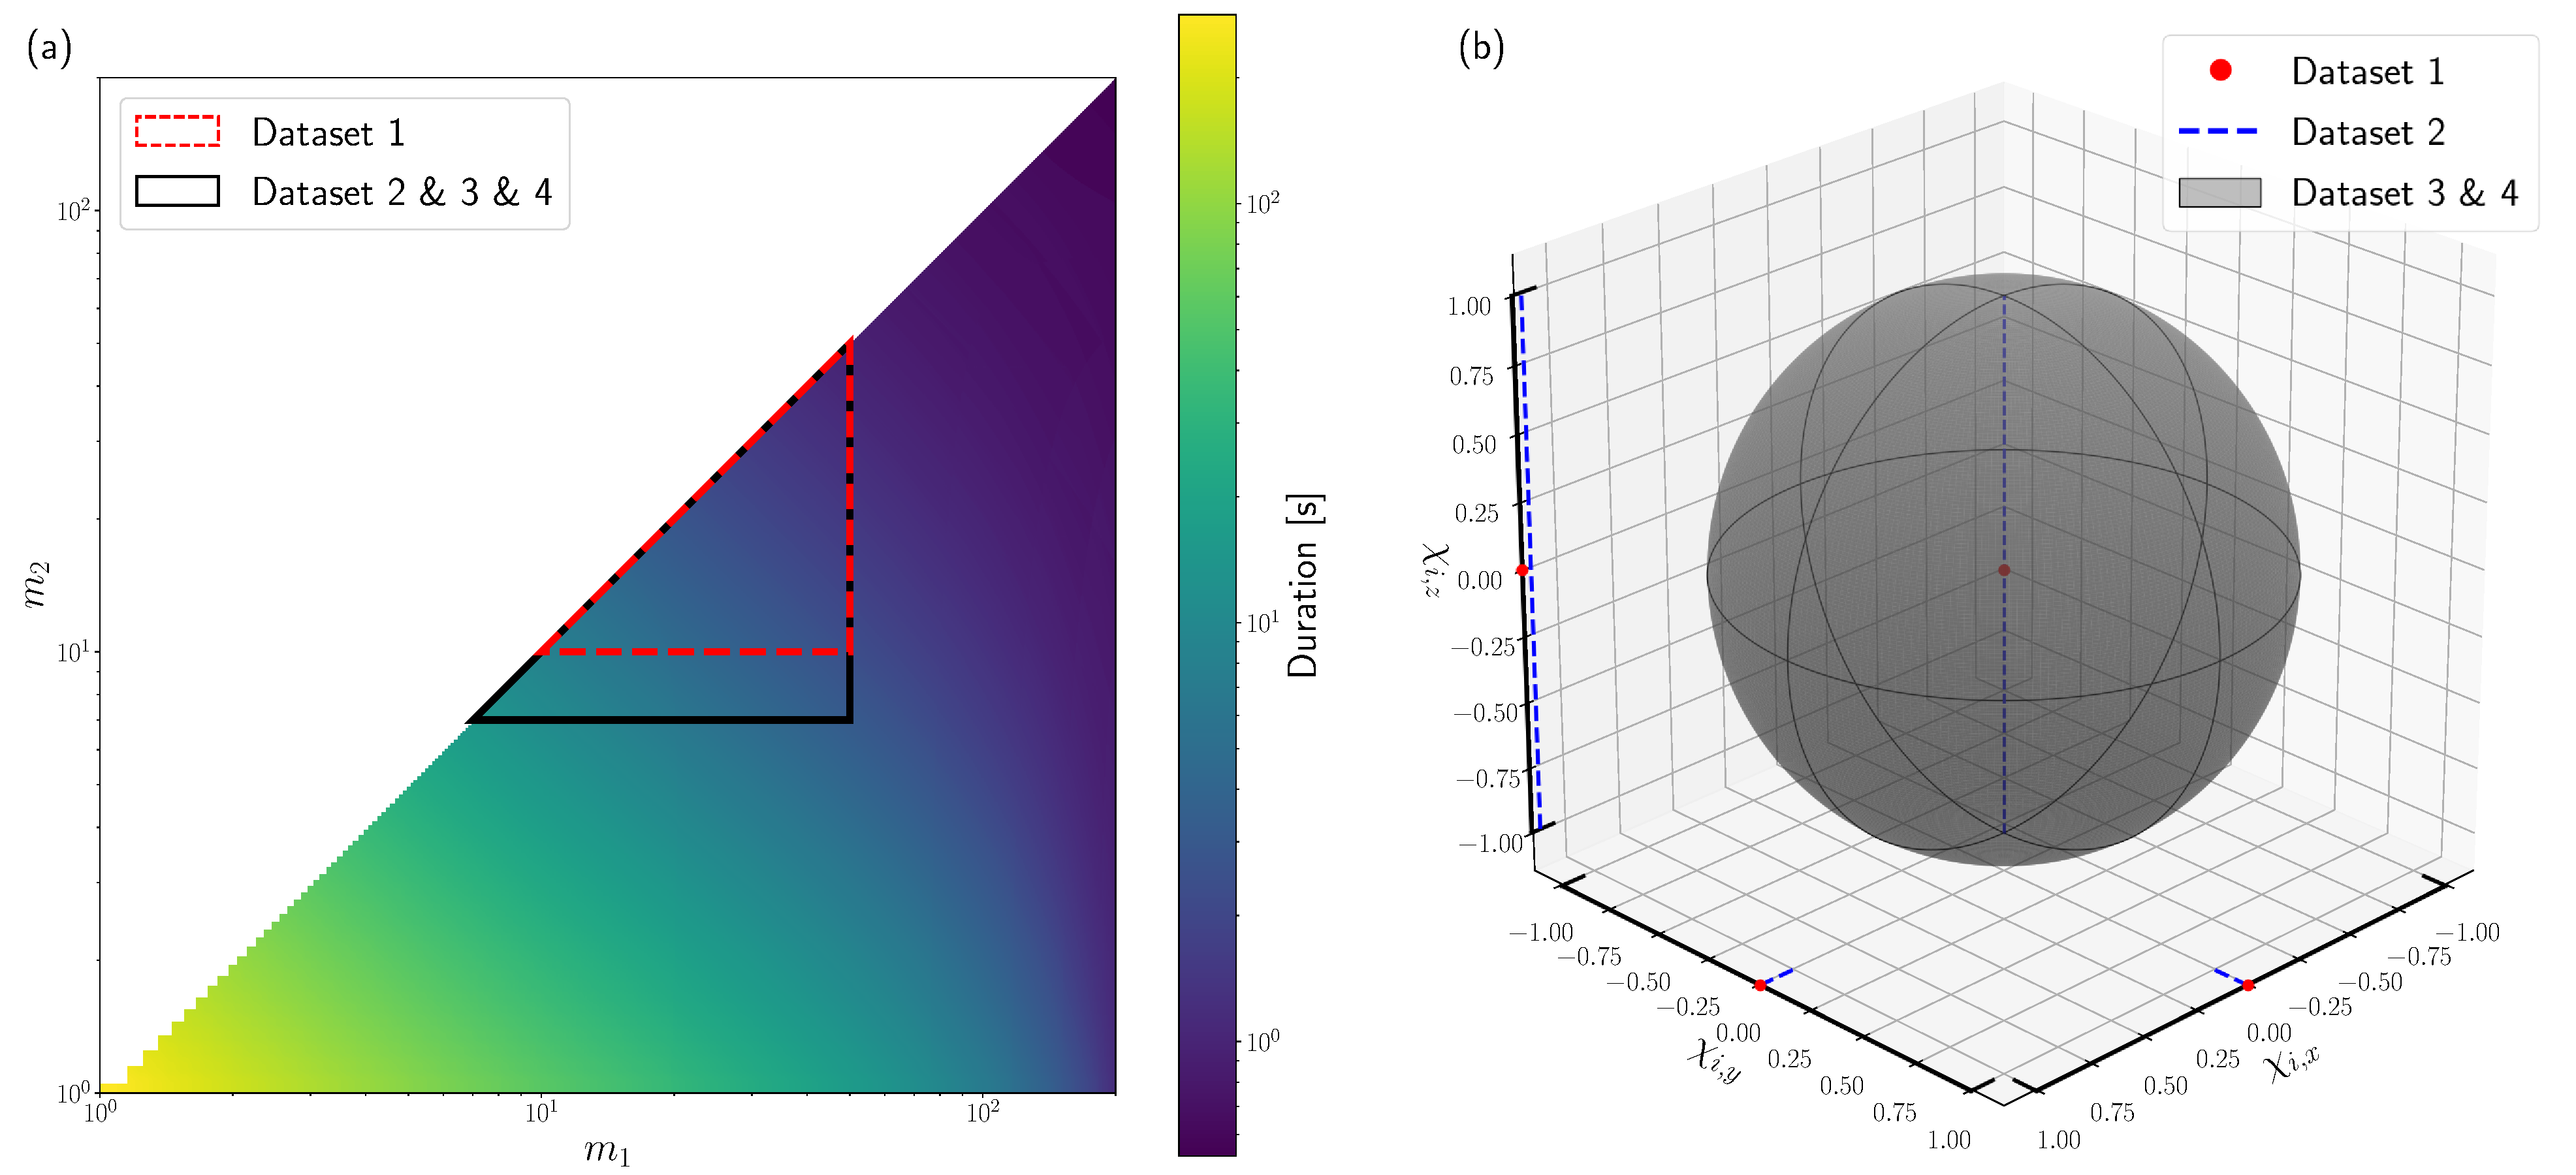
\includegraphics[width=0.98\textwidth]{chapters/mdc/images/combined.pdf}
    \caption[Parameter space]{An illustration of the range for the intrinsic parameters covered by this challenge. The left panel (a) shows a typical range for the component masses used by state of the art searches~\cite{Nitz:2021zwj}. The color indicates the duration of the waveform from \SI{20}{\hertz}. The triangles show the parameter regions covered by this challenge. The right panel (b) shows the component-spin $\chi_i$ distribution of the different datasets in this challenge.}
    \label{fig:parameters}
\end{figure*}

\subsubsection{Dataset 1}
The noise from the first dataset is purely Gaussian and simulated from the \acrshort{psd} model \verb|aLIGOZeroDetHighPower|~\cite{lalsuite} for both detectors. This means that the \acrshort{psd} used to generate the data contains no sharp peaks originating from factors such as the power grid, is the same for all segments, and is known to the participants.

Injected signals are non-spinning and no higher-order modes are simulated. The component masses are uniformly drawn from \SIrange{10}{50}{M_\odot}. We enforce the condition that the primary mass has to be equal or larger than the secondary mass. With this mass range, at a lower frequency cutoff of \SI{20}{\hertz}, and for non-spinning systems the signal duration is on the order of \SI{1}{\second}.

The first dataset represents a solved problem, as it has already been excessively studied in the past~\cite{George:2016hay, Gabbard:2017lja, Schafer:2021cml}. It is meant as a starting point where people new to the field can refer to existing literature to get off the ground initially. We expected many of the algorithms to perform equally well on this set.

The final challenge set for dataset 1 was generated with the seed $1\,068\,209\,514$ and a start time of $0$.

\subsubsection{Dataset 2}\label{sec:data:ds2}
The noise for the second dataset is also purely Gaussian and simulated. However, in contrast to the first dataset the \acrshort{psd}s were derived from real data from \acrshort{o3a} and as such contain power peaks at certain frequencies and are noisy. We generated a total of $20$ \acrshort{psd}s for each detector. The \acrshort{psd}s used to generate the noise are randomly chosen from these lists and as such are unknown to the search algorithm. The lists themselves are known to the participants. The \acrshort{psd}s in both detectors are independent of each other but do not change over time.

Signals are now allowed to have a spin aligned with the orbital angular momentum with a magnitude between $-0.99$ and $0.99$. Additionally, the mass range is adjusted to draw component masses from the range \SIrange{7}{50}{M_\odot}. This change increases the maximum duration of the signals at a lower frequency cutoff of \SI{20}{\hertz} to $\approx$ \SI{20}{\second}. No higher-order modes are simulated for this dataset and due to the aligned spin requirement no precession effects are present in the waveform.

The second dataset was intended to pose a considerable increase in difficulty to the first dataset. Using an unknown \acrshort{psd} which was derived from real data requires participants to estimate it during the analysis, if the algorithm requires it. However, we expected that increasing the signal duration to up to \SI{20}{\second} would be the more prominent reason for an increase in difficulty as many previous machine learning algorithms have had trouble when dealing with large inputs~\cite{Dreissigacker:2020xfr, Schafer:2020kor, Gabbard:2019rde, Goodfellow:2016:DNN}. Finally, we did not expect a large increase in the difficulty of the dataset due to the inclusion of aligned spins.

The final challenge set for dataset 2 was generated with the seed $2\,743\,406\,703$ and a start time of $0$.

\subsubsection{Dataset 3}
The noise for the third dataset is also simulated and purely Gaussian. The increase in difficulty of the noise comes from varying the \acrshort{psd}s over time. Instead of choosing a single random \acrshort{psd} from the list of $20$ \acrshort{psd}s per detector described in \autoref{sec:data:ds2} and generating all noise with that one \acrshort{psd}, the \acrshort{psd} for dataset 3 is randomly chosen for each segment. 

The mass range from \SIrange{7}{50}{M_\odot} and subsequently the maximum signal duration of \SI{20}{\second} is unchanged compared to \autoref{sec:data:ds2}. However, instead of requiring the spins to be aligned with the orbital angular momentum, their orientation is isotropically distributed with a magnitude between $0$ and $0.99$. As a consequence, precession effects are now present in the waveforms. Additionally, we also model all higher-order $(l,m)$-modes available in \verb|IMRPhenomXPHM|, which are: $(2, 2)$, $(2, -2)$, $(2, 1)$, $(2, -1)$, $(3, 3)$, $(3, -3)$, $(3, 2)$, $(3, -2)$, $(4, 4)$, $(4, -4)$~\cite{Pratten:2020ceb}.

The main challenge of this dataset was intended to be the inclusion of precession effects. While these are not as impactful for short duration, high mass systems, they can substantially alter the signal morphology for lower mass systems. Adding higher-order modes can also substantially increase signal complexity. Both of these effects are currently not modeled in any production search relying on accurate signal models, as their inclusion requires an increase in size of the filter bank to include millions of templates~\cite{Harry:2016ijz, Harry:2017weg}. As such, we expected many if not all of the submitted algorithms to struggle with this dataset. On the other hand, any machine learning based algorithm that operates successfully on this dataset may motivate the utilization of machine learning in production searches in the future by extending the searchable parameter space.

The final challenge set for dataset 3 was generated with the seed $470\,182\,217$ and a start time of $0$.

\subsubsection{Dataset 4}
Dataset 4 is the only dataset that contains real detector noise obtained from the Gravitational Wave Open Science Center (\acrshort{gwosc})~\cite{LIGOScientific:2019lzm}. All noise was sampled from parts of \acrshort{o3a} that had the ``data'' quality flag and none of the flags ``CBC\_CAT1'', ``CBC\_CAT2'', ``CBC\_HW\_INJ'', or ``BURST\_HW\_INJ'' were active. We consider only segments where the data from both LIGO Hanford and LIGO Livingston clear the above conditions and excluded \SI{10}{\second} around any detection listed in GWTC-2~\cite{LIGOScientific:2020ibl}. Afterwards we discarded any segments shorter in duration than \SI{2}{\hour}. To allow for different noise realizations, we shift the data from LIGO Livingston by a random time from \SIrange{0}{240}{\second} while keeping the data from LIGO Hanford fixed. The time shifts are independent for each segment and to avoid any possible overlap between neighbouring segments, we consider each segment on its own.

To reduce the amount of data that has to be downloaded by participants we pre-selected the suitable parts of the \acrshort{o3a} data. We then applied a low frequency cutoff of \SI{15}{\hertz} to reduce the dynamic range of the data and multiplied the numerical values by a factor of $\approx 2^{69}$ to allow a lossless conversion to single precision. Finally, the data was converted to single precision and stored in a compressed format. This allowed us to provide a download link to a single file of \SI{94}{\giga\byte} size containing enough data to generate up to \SI{7024699}{\second}$\approx$\SI{81}{\day} of coincident real noise for both detectors. The data was scaled by the constant factor to avoid the loss of dynamic range due to the conversion from double precision to single precision. When generating test data, the data is converted back to double precision and the scaling is inverted. The code used to downsample the data is also open source and available at~\cite{github}.

The signals are generated equivalently to the signals in dataset 3, i.e. masses are uniformly drawn from \SIrange{7}{50}{M_\odot}, spins are isotropically distributed with a magnitude from $0$ to $0.99$, and all higher-order modes available in \verb|IMRPhenomXPHM| are generated. Consequently, precession effects are simulated.

This dataset is intended to be indicative of a real-world application of the search in parameter regions which are currently sparsely searched. Given that many machine learning searches have proven to generalize well from Gaussian noise to real detector noise at higher \acrshort{far}s in the past~\cite{George:2017pmj, Gebhard:2019ldz, Krastev:2020skk, Wei:2020ztw} we expected that machine learning algorithms that do well on dataset 3 will also be competitive for dataset 4. However, it was expected that handling short glitches may prove difficult for certain searches, especially those focusing most on the merger and ringdown.

The final challenge set for dataset 4 was generated with the seed $2\,514\,409\,456$ and a start time of $0$.

\subsection{Evaluation}\label{sec:metrics}
All submissions are evaluated on the challenge sets, which are generated with a seed unknown to the participants at the time of submission. The evaluation is run on the Atlas computing cluster at the Albert-Einstein-Institut (AEI), Hannover. Groups that submitted an algorithm had no direct access to the evaluation stage\footnote{This excludes submissions by the organization group. However, no member of the organization group accessed the challenge-data before the submission deadline or altered their algorithm after the submission deadline.} and final results presented in this work were only communicated back to the groups after the submission deadline had passed.

We compute two metrics for every submission and dataset. These are the wall-clock time required by the algorithm at hand to analyze one month of data as well as the sensitive distance of the search as a function of the false-alarm rate. In essence, the sensitivity as a function of the false-alarm rate is a receiver operating characteristic (\acrshort{roc}) curve that factors in the varying signal strengths of the injected \acrshort{gw}s. It is a common measure of search sensitivity for production \acrshort{gw}-searches~\cite{Usman:2015kfa} and thus allows for easy comparisons. We do not compute the \acrshort{roc} curve directly, for two reasons. First, it requires the number of a negative samples in the data. Since our data is continuous and the evaluation is left to the groups, defining a negative sample is not possible. Second, the \acrshort{roc} curve can be changed by choosing a different signal population. For instance, the \acrshort{roc} curve can be driven to zero by choosing a population of signals that are excessively far from the detectors. The sensitive distance normalizes the data by the injected population.

For the calculation of the sensitive distances we use two challenge sets for each of the 4 datasets. The first contains pure noise and we will call it the background set from here on out. The second contains the same noise as the background set but adds \acrshort{gw} signals into it. This second set will be called the foreground set from here on out. As described in \autoref{sec:submission-req} any search algorithm is expected to process these files and return lists of events, where an event is a combination of a GPS time, a ranking statistic-like quantity, and a value for the timing accuracy. We will call these events background or foreground events when they have been derived from the background or foreground set, respectively. For the remainder of this section we will refer to the ranking statistic-like quantity simply as ranking statistic, to simplify our statements.

To calculate the sensitivity as a function of the false-alarm rate, we need to determine the false-alarm rate as a function of the ranking statistic. Next we can also determine the sensitivity as a function of the ranking statistic. Finally, we can combine the two, by evaluating both at the same values of the ranking statistic.

We use the ranking statistic of all background events as points where both the \acrshort{far} as well as the sensitivity is evaluated. Each of these is certain to be a false positive and thus ensures that the \acrshort{far} is unique at each threshold, as long as the search does not return identical ranking statistics for multiple background events.

To calculate the \acrshort{far} at a given ranking statistic we count the number of background events with a ranking statistic greater than this threshold. We, subsequently, turn that into a rate by dividing the number of false-positives by the duration of the background data, i.e. \SI{2592000}{\second}. With $N_{\text{FP}, \mathcal{R}}$ the number of false-positives at a given ranking statistic $\mathcal{R}$ and $T$ the time spanned by the background set, the \acrshort{far} $\mathcal{F}$ can be calculated by
\begin{equation}
    \mathcal{F} = \frac{N_{\text{FP}, \mathcal{R}}}{T}.
\end{equation}

The sensitive volume of a search at \acrshort{far} $\mathcal{F}$ can be calculated by~\cite{Usman:2015kfa}
\begin{equation}\label{eq:sens-vol-full}
    V\left(\mathcal{F}\right) = \int d\bm{x}d\bm{\Lambda}\ \epsilon\left(\mathcal{F};\bm{x},\bm{\Lambda}\right)\phi\left(\bm{x},\bm{\Lambda}\right),
\end{equation}
where $\bm{x}$ are the spatial coordinates of the injection, $\bm{\Lambda}$ are the injection parameters, $\epsilon\left(\mathcal{F};\bm{x},\bm{\Lambda}\right)$ is the efficiency of the search at \acrshort{far} $\mathcal{F}$, and $\phi\left(\bm{x},\bm{\Lambda}\right)$ is the distribution of the injection parameters $\bm{x}$ and $\bm{\Lambda}$.

When injections are performed uniformly in volume up to a maximum distance $d_\text{max}$, \autoref{eq:sens-vol-full} can be approximated by~\cite{Usman:2015kfa}
\begin{equation}\label{eq:sens-vol-approx-1}
    V\left(\mathcal{F}\right)\approx V\left(d_\text{max}\right)\frac{N_{I,\mathcal{F}}}{N_I},
\end{equation}
where $ V\left(d_\text{max}\right)$ is the volume of a sphere with radius $d_\text{max}$, $N_{I,\mathcal{F}}$ is the number of found injections at a \acrshort{far} of $\mathcal{F}$, and $N_I$ is the total number of injections performed. An injection is found if there is at least one foreground event that is within $\pm \Delta t$ of the injection, where $\Delta t$ is the time variance assigned to the event by the search algorithm. The number of found injections at a given \acrshort{far} considers only those foreground events where the ranking statistic assigned to the specified event is greater than the ranking statistic corresponding to the \acrshort{far}. In machine learning terms \autoref{eq:sens-vol-approx-1} is the recall at a given threshold on the network output multiplied by the volume of a sphere with radius $d_\text{max}$, assuming that each injection corresponds to exactly one true positive.

However, the injections in the datasets are not performed uniformly in volume, as we sample over the chirp-distance instead of the luminosity distance. The chirp-distance is given by~\cite{LIGOScientific:2007npa}
\begin{equation}
    d_c = d{\left(\frac{\mathcal{M}_{c,0}}{\mathcal{M}_c}\right)}^{5/6},
\end{equation}
where $d$ is the luminosity distance, $\mathcal{M}_c = {\left(m_1 m_2\right)}^{3/5} / {\left(m_1 + m_2\right)}^{1/5}$ is the chirp mass, and $\mathcal{M}_{c,0} = $\SI[parse-numbers=false]{1.4/2^{1/5}}{M_\odot} is a fiducial chirp mass used as a basis for calculation. Note that in contrast to \cite{LIGOScientific:2007npa} we use the luminosity distance instead of the effective distance as our basis.

When sampling the injections from the distributions defined in \autoref{tab:shared_params} using the chirp-distance, effectively the maximum luminosity distance $d$ is selected based on the chirp mass; the smaller the chirp mass, the smaller the maximum luminosity distance at which injections are placed. This allows us to increase the number of detectable low mass systems and, subsequently, make statistically meaningful statements about the sensitivity for these systems without requiring a large increase in the amount of data that needs to be analyzed. However, when considering a fixed chirp mass, injections are still placed uniformly within that sphere of the adjusted maximum luminosity distance. In \autoref{eq:sens-vol-approx-1} we assumed that each injection was placed uniformly within the volume spanned by the sphere with volume $V\left(d_\text{max}\right)$. To adjust it for sampling over luminosity distance we have to factor in that the probed distance depends on the selected chirp mass. We, therefore, find
\begin{equation}
     V\left(\mathcal{F}\right)\approx \frac{V\left(d_\text{max}\right)}{N_I}\sum_{i=1}^{N_{I,\mathcal{F}}} \frac{V\left(d_{c,\text{max}} {\left(\frac{\mathcal{M}_{c, i}}{\mathcal{M}_{c,0}}\right)}^{5/6}\right)}{V\left(d_{c,\text{max}} {\left(\frac{\mathcal{M}_{c, \text{max}}}{\mathcal{M}_{c,0}}\right)}^{5/6}\right)},
\end{equation}
where $\mathcal{M}_{c,i}$ is the chirp mass of the $i$-th found injection, $d_{c,\text{max}}$ is the upper limit on the injected chirp distances, and $\mathcal{M}_{c,\text{max}}$ is the upper limit on the injected chirp masses. This expression can be simplified to yield
\begin{equation}
     V\left(\mathcal{F}\right)\approx \frac{V\left(d_\text{max}\right)}{N_I}\sum_{i=1}^{N_{I,\mathcal{F}}} {\left(\frac{\mathcal{M}_{c, i}}{\mathcal{M}_{c, \text{max}}}\right)}^{5/2},
\end{equation}
which is the formula we use to estimate the sensitive volume of a search algorithm. Instead of quoting the volume directly we convert it to the radius of a sphere with the corresponding volume and quote that instead.

We also measure the time the algorithm requires to evaluate an entire month of test data. Since all machine learning search algorithms are running on the same hardware these values can be used to compare the speed of the different analyses on the given hardware. For a summary of the available hardware resources please refer to \autoref{tab:hardware}. However, we expect the computational time to be dominated by pre-processing steps, which can in theory be heavily optimized. For this challenge, though, we did not expect many submissions to invest resources into optimizing their pre-processing and thus advise the reader to not overemphasize the provided numbers.

\begin{table}[]
    \centering
    \begin{tabularx}{0.98\textwidth}{XX}
    \hline\hline
    Hardware type & Specification \\
    \hline
    CPU & $2\times$ Intel Xeon Silver 4215, 8(16) cores(threads) at \SI{2.5}{\giga\hertz} \\
    GPU & $8\times$ NVIDIA RTX 2070 Super (\SI{8}{\giga\byte} VRAM) \\
    RAM & \SI{192}{\giga\byte} \\
    \hline\hline
    \end{tabularx}
    \caption[Hardware specifications]{Main hardware specifications available to each search algorithm during final testing.}
    \label{tab:hardware}
\end{table}

All runtimes are measured twice; once for the foreground set and once for the background set. In both cases the wall-time that has passed between calling the executable and it returning is measured.

\subsection{Submission Requirements}\label{sec:submission-req}
All submissions are provided with the path to a single file containing the input data they have to process. In particular they have to be able to read HDF5 files, the structure of which is detailed in \autoref{sec:data}. Importantly, no pre-processing other than the introduction of a low frequency cutoff of \SI{15}{\hertz} has been applied to the data. All other pre-processing has to be performed by the algorithms themselves. In addition to the path to the input data, each algorithm is provided with a second path at which it is expected to store a single HDF5 file. This file has to contain three one-dimensional datasets of equal size named ``time'', ``stat'', and ``var''.

The ``time'' dataset is expected to contain the GPS times at which the algorithm predicts a \acrshort{gw} signal to be present. These are compared to the injection times to determine which injections were found, which were missed, and how many false positives the analysis produced.

The ``stat'' dataset is expected to contain a ranking-statistic like quantity for every GPS time in the ``time'' dataset. Here, ranking-statistic like quantity means a value where larger numbers indicate a higher degree of believe for the search to have found a \acrshort{gw} signal. Having a ranking-statistic like quantity associated to all candidate detections enables us to assign a statistical significance to any event.

The ``var'' dataset is expected to contain the estimated timing accuracy of the search algorithm for all GPS times in the ``time'' dataset. This value determines the window around the GPS time returned by the search within which an injection has had to be made in order to consider the detection a true positive and the injection to be found. This value may be constant for all times at which the search expects to have seen a signal. We allowed searches to specify this value themselves, as we felt it to be unsuitable for a signal detection challenge to require a fixed timing accuracy. In principle, this freedom can be abused by choosing an accessively high value of $\Delta t$ and claiming all events as true positives. However, all groups have chosen values on similar scales and more importantly far shorter than the average separation of two injections.

Throughout the paper, we will refer to events returned by the search. By that we mean a single tuple $\left(t, \mathcal{R}, \Delta t\right)$ contained in the ``time'', ``stat'', and ``var'' datasets, respectively.

To be able to execute all algorithms without major problems, we ask participants to either provide a single executable that can be run on the Linux command-line utilizing only the provided software stack or to provide a singularity image that we can execute. In both cases the algorithms have to accept two positional command line arguments; the path to the input data file and the path at which the output file should be stored. The main Python packages available to submitted executables are listed in \autoref{tab:software}, for a full list refer to \cite{github}.

\begin{table}[]
    \centering
    \begin{tabularx}{0.48\textwidth}{XX}
        \hline\hline
        Python package & Version \\
        \hline
        bilby & 1.1.3 \\
        pycbc & efeaeb6 \\
        tensorflow-gpu & 2.6.0 \\
        tensorflow-probability & 0.14.0 \\
        torch & 1.9.1+cu11 \\
        \hline\hline
    \end{tabularx}
    \caption[Core software stack]{A selective list of the core Python packages available to algorithms during evaluation. A complete list is given at~\cite{github}.}
    \label{tab:software}
\end{table}

Each algorithm is executed by hand and closely monitored by the organization team of the challenge. Participants are not allowed to directly tune or influence the final evaluation.

To ensure that participants have submitted the correct version of their algorithm and to make sure that their algorithm behaves as expected on the evaluation hardware and software, all algorithms are first evaluated on a validation set which is generated equivalently to the final test set. The results on this validation set are then communicated back to the submitting group. Once the group has approved that their algorithm performs within the expected margin of error, the algorithm is applied to the real challenge sets. These challenge sets are the same for all participants and were kept secret until the deadline for final submissions had passed.

Since multiple members of the organization team have submitted algorithms to this challenge, the challenge datasets were only generated after the submission deadline had passed. The script to generate test data provides an option to use a random seed. This option was used to generate the final challenge datasets and ensures that no submission had knowledge of the challenge set prior to the submission deadline.

We allowed all participants to retract their submissions at any point prior to the final publication of our results. This means that participants were allowed to retract their submissions even after they were informed about the performance of their algorithm on the final challenge sets and after they have seen the performance of other entries. No group made use of this freedom and retracted their submission after results were internally published.


\section{Submissions}\label{sec:submissions}
In this section we briefly introduce the different algorithms. For more details on the individual submissions we refer the reader to the original works cited within each subsection. The subsections are titled by the group name and are given in order of registration to the challenge.

All algorithm preparation was performed by the individual groups using their own available hardware resources. This crucially includes training of machine learning algorithms, for which no resources were provided by the organizers of this challenge. There were no strict requirements to submit algorithms that are based on machine learning techniques. We even encouraged the submission of a few traditional algorithms to quote a point of reference. However, the available resources detailed in \autoref{sec:metrics} for evaluation of the test sets are tailored to suit the needs of machine learning algorithms.


\subsection{MFCNN}\label{sec:submission-mfcnn}
\footnote{The corresponding authors for the MFCNN submission are He Wang, Shichao Wu, Zong-Kuan Guo, Zhoujian Cao, and Zhixiang Ren.}
The submission of the MFCNN group is based on the works from He et al.~\cite{Wang:2019zaj}. The authors of \cite{Wang:2019zaj} refer to the model as matched-filtering convolutional neural network (MFCNN). MFCNN is a semi-coherent search model. The basic idea of the model is to use waveform templates as learnable weights in neural network layers. Analogously to the standard coincident matched-filtering searches the output of each matched-filtering layer is maximized and normalized in the unit of matched-filtering \acrshort{snr}s for each \acrshort{gw} detector. However, triggers are not generated on a single detector. The remaining part of the neural network is a usual convolutional neural network that is employed afterwards to jointly analyze the output from all detectors. Finally, a SoftMax function is applied to evaluate the confidence score of a \acrshort{gw} signal being present in the \acrshort{gw} detector network. The architecture was designed to take the advantages of both matched-filtering and convolutional neural networks and combine them to search for real \acrshort{gw} events in GWTC-1~\cite{LIGOScientific:2018mvr}. To adapt to this challenge, the source code~\cite{Wang:2022aaa} of the submission was translated from the MXNet framework~\cite{Chen:2015aaa} used in the original work to a PyTorch~\cite{Paszke:2019aaa} implementation.

The training data for the model is generated by the code that generates dataset 4. The training data are input into the model directly with none of the usual pre-processing such as band-pass or whitening, which is consistent with the original work~\cite{Wang:2019zaj}. In fact, the model is equipped with a whitening layer to estimate the power spectrum for each input data. The main modification used in this challenge is to randomly sample 25 templates in the first matched-filtering layer from the same parameter space used in dataset 4 of this challenge. It performs significantly better than the original gridded and fixed template configuration. The subsequent convolution network of the model is constructed using the current excellent lightweight models MobileNetV3~\cite{Howard:2019aaa} which give state-of-the-art results in major computer vision problems. The submission uses curriculum learning, during which the model is trained with decreasing multiples of signal amplitude. The multiplicative factor is lowered from 50 to 1 until convergence. Multiple models were randomly initialized and trained on a NVIDIA Tesla V100 GPU, from which the best was chosen for this submission.

To search for triggers and evaluate the performance of the model, a sliding window approach is implemented. The evaluation data is divided into overlapping segments corresponding to the input size of the model. Subsequently, all segments are passed through the model resulting in a sequence of predictions and a table of \acrshort{snr} peaks from the 25 sorted matched filters. The step size is 1 second and a threshold of 0.5 is set on the network output as in~\cite{Wang:2019zaj}. The ``time''-, ``var''- and ``stat''- dataset of the output file described in \autoref{sec:submission-req} are derived from the table of \acrshort{snr} peaks associated with directly filtering the templates with the data. The GPS time and time variance of each trigger are designated as the median value and the interquartile range of \acrshort{snr} peaks from the nearby segments, respectively. We count the coincident \acrshort{snr} peaks between two detectors to quantify the ranking-statistic. Other experiments are still in progress and are supposed to be published alongside further details in a standalone paper.

The final version of the algorithm submitted by the \mfcnn group was provided after the submission deadline had past. A vital flaw in their original contribution was discovered and was allowed to be fixed.


\subsection{PyCBC}\label{sec:submission-pycbc}
\footnote{The corresponding author for the PyCBC submission is Alexander H. Nitz.}
The \textit{PyCBC} submission is based on a standard
configuration of the PyCBC-based archival search 
for compact-binary mergers~\cite{Nitz:2021zwj}. The search infrastructure was used, in addition to cWB, for the first detection of gravitational waves, GW159014~\cite{LIGOScientific:2016aoc}, in production analyses by multiple groups to produce gravitational-wave catalogs~\cite{LIGOScientific:2021djp, Nitz:2021zwj} and targeted analyses~\cite{Nitz:2019spj}. A similar low-latency PyCBC-Live analysis is also based around the same toolkit~\cite{Nitz:2018rgo,DalCanton:2020vpm}. The analysis uses matched filtering to identify candidate observations in combination with a bank of predetermined waveform templates that correspond to the expected gravitational-wave signals~\cite{Allen:2005fk}. Matched filtering is known to be the optimal linear filter for stationary, Gaussian noise. To account for the potential non-Gaussian noise transients~\cite{Nuttall:2015dqa,Cabero:2019orq,Davis:2022dnd}, each candidate and the surrounding data are checked for consistency with the expected signal~\cite{Allen:2004gu,Nitz:2017lco}. In addition, the properties of candidates, such as their time of arrival, amplitude, and phases in each detector are checked for consistency with an astrophysical population~\cite{Nitz:2017svb}. 

The empirically measured noise distribution and the consistency with the expected gravitational-wave signal are combined to calculate a ranking statistic for each potential candidate~\cite{Nitz:2017svb, Davies:2020tsx}; this ranking statistic is used as the ``stat'' value of dataset output, along with its associate trigger time in ``time''. The ``var'' dataset is set to a constant of \SI{0.25}{\second}. Two template banks
are used for the submitted results. For dataset 1, a template bank of non-spinning
waveform templates, using the IMRPhenomD~\cite{Husa:2015iqa} model, is created using stochastic placement. Datasets 2, 3, and 4 were evaluated with a common template bank that includes templates that account for spin which is aligned with the orbital angular momentum. Furthermore, only the dominant mode of the gravitational-wave signal was used and effects such as precession were not accounted for. In both cases, the mass boundaries of the template bank conform to the challenge set parameters.

The final version of the algorithm submitted by the \pycbc group was provided after the submission deadline had past. A vital flaw in their original contribution was discovered and was allowed to be fixed. Furthermore, the \pycbc submission strictly speaking uses a different algorithm for dataset 1 than for all other datasets, as the template banks are not the same. The change in template banks was accepted, as this work does not focus on a runtime analysis.


\subsection{CNN-Coinc}\label{sec:submission-cnn}
\footnote{The corresponding author for the CNN-Coinc submission is Marlin B. Sch{\"a}fer.}
This submission is based on the works from Gabbard et al.~\cite{Gabbard:2017lja} and Sch\"afer et al.~\cite{Schafer:2021cml}. It utilizes the network architecture presented in~\cite{Gabbard:2017lja} with a prepended batch-normalization layer~\cite{Ioffe:2015aaa}. As such the network processes $8\,192$ input samples, which corresponds to \SI{4}{\second} at a sampling rate of \SI{2}{\kilo\hertz}. The network is trained only once and applied to the data from both detectors individually. Afterwards the outputs are correlated to find coincident events as detailed in~\cite{Schafer:2021cml}. The source code for training the network and applying it to test data of the format used in this challenge is open source and can be found at~\cite{githubCnnCoinc}. The algorithm was designed to enable an easy and efficient estimation of the search background by applying time shifts between the individual detectors data. While this feature cannot be utilized in this challenge, the original paper~\cite{Schafer:2021cml} highlights the advantages of this approach.

The network is trained on parts of the real \acrshort{o3a} noise from the Hanford detector as provided in this challenge. Signals are generated using the waveform approximant \verb|IMRPhenomXPHM|~\cite{Pratten:2020ceb} from the same parameter distribution used in datasets 3 and 4 in this challenge. Merger times of the signals are varied between \SIrange{2.9}{3.1}{\second} from the start of the input window of the network. The signals are pre-whitened by one of the provided Hanford \acrshort{psd}s used in datasets 2 and 3. Noise samples are non-overlapping parts taken from the real noise data provided by this challenge, where each segment is whitenened by an estimate of the \acrshort{psd} on that segment. The network was trained for 100 epochs using the loss and optimizer settings provided in~\cite{Schafer:2021cml} on a single NVIDIA RTX 2070. The epoch with the greatest binary accuracy on a single training run was chosen for this challenge.

During evaluation the network is applied to the challenge-data using a sliding window approach. Each data segment is whitened by an estimate of the \acrshort{psd} of that segment obtained by Welch's method~\cite{Allen:2005fk, Welch:1967aaa}. All data is whitened before the network is applied for computational efficiency. Subsequently, the network is applied to the data via a sliding window with a step size of $204$ samples \SI[parse-numbers=false]{\approx 0.1}{\second}. Afterwards a threshold of $3.4$ is applied on the unbounded Softmax replacement (\acrshort{usr}) output, which was introduced in~\cite{Schafer:2021fea}. Coincident events are calculated using the same procedure and parameters as outlined in~\cite{Schafer:2021cml}. The ``time''- and ``stat''-dataset of the output file described in \autoref{sec:submission-req} list the coincident event times and ranking statistic values, respectively. The time variance of the ``var''-dataset is set to a constant value of \SI{0.3}{\second}.


\subsection{TPI FSU Jena}\label{sec:submission-jena}
\footnote{The corresponding authors for the \jena submission are Ond{\v{r}}ej Zelenka, Bernd Br{\"u}gmann, and Frank Ohme.}
This submission closely followed the method of \cite{Schafer:2021fea}, which is itself based on~\cite{Gabbard:2017lja}, with several modifications to adapt to the specifics of the challenge. The core of the algorithm is a convolutional neural network that accepts a $2\times 2048$ input tensor corresponding to 1 second of data from 2 detectors sampled at \SI{2048}{\hertz}. Its architecture is derived from that of \cite{Schafer:2021fea} and deviates from the original network by a larger size of the individual layers and a doubled number of convolutional layers. These modifications are the result of a hyperparameter variation experiment which found these settings to be optimal. A standalone publication on this submission giving further details on the methodology is in preparation. The final layer of the network is a Softmax layer over two inputs which is used for training and removed using the \acrshort{usr} \cite{Schafer:2021fea} during evaluation.

The network is trained on a dataset constructed by whitening a randomly chosen part of the real noise file and slicing it to produce 1-second noise samples and injecting whitened \texttt{IMRPhenomXPHM}-generated BBH waveforms into half the noise samples at \acrshort{snr}s uniformly drawn between $7$ and $20$. The waveform parameters are drawn from the same distributions as are used in dataset 4 of this challenge. The training dataset consists of $10^6$ samples and the validation set of $2\cdot 10^5$ samples.

During evaluation, each segment in the input file is whitened separately using the estimated \acrshort{psd} and sliced into 1-second segments at 0.1-second spacing. These are fed to the network with the \acrshort{usr} applied. First-level triggers are selected by applying a threshold of -8, which are then clustered into events. For each event, the ``time'' and ``stat'' in the output file are the values of the highest ranking statistic first-level trigger of each cluster, and ``var'' is set to $0.2$ seconds. The algorithm is implemented using the PyTorch framework~\cite{Paszke:2019aaa} and spawns child processes to whiten individual segments. The network evaluation is performed by the parent process.


\subsection{Virgo-AUTh}\label{sec:submission-auth}
\footnote{The corresponding authors for the \virgo submission are Paraskevi Nousi, Nikolaos Stergioulas, Panagiotis Iosif, Alexandra E. Koloniari, Anastasios Tefas, and Nikolaos Passalis.}
This submission is based on a simple per-dataset binary classification scheme. Interestingly, it was found that training a model only on dataset 2 or only on dataset 4 can yield impressive results on the other datasets as well. Specifically, training samples from dataset 2 can generalize well to dataset 3 and 1 and not so well on dataset 4, whereas training samples from dataset 4 can generalize well on datasets 1, 2 and 3. Thus, training samples were only generated from dataset 4. An adaptive normalization mechanism \cite{passalis2019deep} was used instead of batch normalization as the first layer, to handle non-stationary timeseries. For the neural network architecture a deep, ResNet-like model \cite{He:2015aaa} with a depth of 54 layers was used.

One week of training data per dataset was generated and the generated injection parameters were used to construct all corresponding waveforms. This amounted to about 600k background segments of duration \SI{1.25}{\second} with a stride of \SI{2}{\second} between, i.e. the next sample starts \SI{0.75}{\second} after the end of the previous one, and about 580k waveforms, of which 300k were used for the injections. For validation, one day of data was used, resulting in about 86k noise segments and 3.2k waveforms. The noise segments and waveform segments are combined online during training, in a static manner, both for the training and for the validation sets. The input samples are whitened before feeding them to the classifier. The \acrshort{psd} is computed online per batch of \SI{4.25}{\second} with a stride of \SI{3.1}{\second}, and each \SI{1.25}{\second} segment inside this duration is whitened with the same \acrshort{psd}. To increase speed, the Welch method for computing the \acrshort{psd} was implemented in PyTorch~\cite{Paszke:2019aaa} and whitening is implemented as the first layer of the final detection module. Notably, this approach of computing the \acrshort{psd} for every \SI{4.25}{\second} and whitening each \SI{1.25}{\second} segment in a sliding window manner was found to be faster than using a precomputed \acrshort{psd} for every \SI{1.25}{\second} (about $40\%$ faster for one month of data). After whitening, the first and last \SI{0.125}{\second} (\SI{0.25}{\second} total) are removed from each sample.

The best results were obtained with a ResNet-52 type network. A Deep Adaptive Input Normalization (DAIN) layer \cite{passalis2019deep} was used as the first layer after whitening, to handle distribution shifts that may be present. The final output is binary, i.e., noise plus waveforms or noise only, and the objective function used was a regularized binary cross entropy. The ``var'' parameter is set to \SI{0.3}{\second}, as the network predictions are high even when the time of coalescence is slightly outside the preset range. The ``stat'' parameter is set to the network confidence, i.e., a value in the $[0, 1]$ interval corresponding to the probability that a waveform is present. Finally, \SI{0.125}{\second} are added to the expected time of coalescence to account for the time lost in the whitening process.

A standalone publication on the methods used in this submission is in preparation.

\subsection{cWB}\label{sec:submission-cwb}
\footnote{The corresponding authors for the \cwb submission are Francesco Salemi, Gabriele Vedovato, Sergey Klimenko, and Tanmaya Mishra.}
Coherent WaveBurst (\cwb) is a waveform model-agnostic search pipeline for \acrshort{gw} signals based on the constrained likelihood method \cite{SoftX, zenodo, cWBhomepage}. The \cwb pipeline has been used for the analysis of scientific data collected by the LIGO-Virgo detectors,  targeting detection of signals from generic \acrshort{gw} sources, including the compact binary mergers~\cite{LIGOScientific:2021djp}.

The \cwb algorithm identifies the excess-power events in the time-frequency domain representation of strain data from multiple detectors~\cite{Klimenko:2015ypf,Klimenko:2004qh}. For each event, the \cwb pipeline reconstructs the \acrshort{gw} waveforms and estimates summary statistics which describe generic properties of the events like the coherence across the detector network, signal strength, and the time-frequency structure.
 
Recently, a boosted decision-tree algorithm, eXtreme-Gradient Boost (XGBoost)~\cite{XGBoost}, was adopted and implemented within the \cwb framework to automate the signal-noise classification of the \cwb events~\cite{Mishra:2021tmu}. Two types of input data are used for the supervised training: signal events (from simulations) and noise events (from background estimations). For each of those, a subset of \cwb summary statistics is fed to XGBoost as input features to train a signal-noise model.  
As in ~\cite{Mishra:2021tmu}, the detection statistic for the machine learning-enhanced \cwb algorithm is defined by:
\begin{equation}\label{eq:x}
	\eta_\mathrm{r} = \eta_\mathrm{0}\cdot W_{\mathrm{XGB}}, 
\end{equation}
where, $\eta_\mathrm{0}$ is {\cwb}s ranking statistic, and $W_{\mathrm{XGB}}$ is the penalty factor calculated by XGBoost ranging between 0 (noise) and 1 (signal). 

This methodology has been recently used in the full reanalysis of publicly available strain data from Advanced LIGO’s Hanford and Livingston third observational run~\cite{Mishra:2022ott}: the machine learning-enhanced \cwb outperforms the standard human-tuned signal-noise classification used for detection of the compact binary coalescences in the \acrshort{o3} run.

For this study, we chose to use machine learning-enhanced \cwb; however, \cwb typically rejects weak candidate triggers (i.e., with \acrshort{far} $\gg 1$ per year) at early production stages. Moreover, the whole workflow is optimized for a trigger production which saturates at \acrshort{far}~$\approx 30 \text{ to } 50$ per month.  Therefore, we modified \cwb to increase the event production rate by almost 2 orders of magnitude: the result is a \cwb with sub-threshold capabilities, able to speed up computation and reduce memory allocations.

While trying to provide the most ``generic'' result for this study, it was decided to re-use the XGBoost model which was developed for ~\cite{Mishra:2022ott}: it should be noted that the model was trained on noise and signal events sets that differ substantially from those adopted for the data sets prepared for \acrshort{mlgwsc1}. The noise backgrounds for dataset 3 and dataset 4 appear to be significantly quieter than \acrshort{o3}. Also, the signals were drawn from a spin-aligned stellar-mass \acrshort{bbh}s population model with different component mass ranges~\cite{PowerLawPeak} and with SEOBNRv4 waveforms ~\cite{Bohe:2016gbl}.
The above-mentioned detection statistic, $\eta_\mathrm{r}$, is used as the ``stat'' value of dataset output, along with its associated trigger peak-time in ``time''. The ``var'' dataset is set to a constant of \SI{0.25}{\second}.

The results from the \cwb group were provided after the submission deadline had passed. The group assured that no tuning to the challenge set was performed.


\section{Data release}
We provide all source code as well as the evaluation results for all submissions at \cite{github}. The repository contains all code accessible to the participants of the challenge, which most importantly  includes a script to generate data and one to produce the sensitivity statistics we provide in \autoref{sec:results}. The repository also contains code for basic visualization as part of the ``contributions'' folder. Adaption of these scripts were used to create the graphics in this paper. The challenge used the code of release 1.3 of the repository.

Alongside the code provided by the challenge organizers we publish the source code that was used to run the contributions for the groups \pycbc, CNN-Coinc, \jena, and \virgo in the ``submissions'' folder of \cite{github}. The submission code for the MFCNN group can be found at \cite{Wang:2022aaa}.

All analysis output files for all submissions created by our analysis are also publicly available and are stored in the ``results'' folder in \cite{github}. For each group we make available the raw output on the foreground and the background for all 4 datasets. Additionally, all timing information is available. The exception is the \cwb group, for which only results on datasets 3 and 4 are available. 

The repository \cite{github} also contains plots used in this paper for all groups, including versions we have not shown here. They can be found in the ``plots'' folder.


\section{Results and discussion}\label{sec:results}
In this section we provide the results of our evaluation process described in \autoref{sec:mlgwcs_methods} for all $6$ submissions. We calculate and discuss sensitive distances, found-missed plots, and runtimes to provide a quantitative comparison between the different submissions. We specifically focus on the difference between machine learning and traditional algorithms and reason where the core differences in performance arise.

The four datasets we use in this study were chosen to answer different questions and serve different purposes. Dataset 1 was meant as an entry point to the challenge that represents a largely solved case~\cite{George:2016hay, Gabbard:2017lja, Schafer:2021cml}. We expected most submissions to perform very similarly on this dataset. The second dataset was intended as the first major step in difficulty. We expected its main challenge to be the longer duration of the injected signals, as many machine learning algorithms target shorter durations and struggle with large analysis segments~\cite{Goodfellow:2016:DNN, Schafer:2020kor}. Dataset 3 includes precession and higher order mode effects in the injected signals that traditional, modeled searches are not optimized for\footnote{A full search of the entire \acrshort{o3} data that includes higher order modes has been performed in \cite{Chandra:2022ixv}.}~\cite{Harry:2016ijz, Harry:2017weg, Dhurkunde:2022aek}. We wanted to test if machine learning algorithms could get closer in performance, or even outperform, the traditional searches in these regions. The intention of dataset 4 was to provide a challenge that is representative of a realistic search on real detector data and a limited parameter space. The data contains non-Gaussian noise artifacts, that can mimic \acrshort{gw} signals~\cite{LIGOScientific:2014qfs, LIGOScientific:2016gtq, LIGOScientific:2019hgc, Davis:2022cmw}, which are strongly suppressed by sophisticated algorithms in traditional searches~\cite{Usman:2015kfa, Messick:2016aqy, LIGOScientific:2019hgc}. Most machine learning algorithms that target real noise do not make use of such noise-mitigation strategies and instead rely solely on the ability of the machine learning algorithm to identify noise artifacts. This approach was reported to be effective for higher \acrshort{far}s in the past~\cite{George:2017pmj, Gebhard:2019ldz, Krastev:2020skk, Wei:2020ztw} and we were, therefore, expecting relatively minor difference between dataset 3 and dataset 4. Furthermore, most traditional algorithms use matched filtering, which is only proven to be optimal for signal recovery when the noise is stationary and Gaussian. Since neither of the two assumptions are true for real detector data, we were also interested to test if machine learning algorithms can perform better than these searches by learning a better noise representation.

\subsection{Sensitivities}
In this subsection we discuss the sensitive distances of the different submissions, which are a measure for how many sources can be detected at any given level of certainty, i.e. at a particular \acrshort{far}. They are the core metric to determine the quality of any search. We focus on the low \acrshort{far} region and truncate the plot at a \acrshort{far} of $10^3$ per month. We chose this cutoff for two reasons. First, to function as a standalone search, algorithms may only report events with low \acrshort{far}s. State of the art pipelines send out alerts only when the \acrshort{far} is smaller than $\mathcal{O}\left(1\right)$ per month~\cite{Nitz:2018rgo}. Second, for high \acrshort{far}s a non-negligible number of detections originate from false associations. This means that a large number of triggers that originate from random noise coincidences are close enough to an injection to be counted as true positives.

Since all machine learning submissions chose to optimize for dataset 4, results on all prior sets also test the capability of generalizing to different signal (sub)populations. Dataset 3 is a special case, as it uses the same distribution to draw the parameters of the injected signals as dataset 4. It, therefore, differs only in the noise contents and is a good test of the performance difference of different algorithms between simulated and real noise.

The results of this challenge are summarized in \autoref{fig:mlgwsc_sens} and \autoref{tab:res}. The four individual panels of \autoref{fig:mlgwsc_sens} show the sensitive distances as a function of the \acrshort{far} for all submissions. The panels contain the results for dataset 1 to 4 from left to right and top to bottom. The errors on the sensitive distances estimated from the variance of the Monte-Carlo integration are smaller than \SI{80}{\mega\parsec} for all curves. In \autoref{tab:res} we give the numeric values for the sensitive distances at three selected \acrshort{far} values of $1$, $10$, and $100$ per month for all submissions and datasets. We also provide information on the wall-clock time used to evaluate the different sets. Due to time constraints, we only show sensitivity curves for dataset 3 and 4 for the submission from the \cwb group. We also note that \pycbc used a different template bank to analyze dataset 1 than for the remaining three datasets.

\begin{figure*}
    \centering
    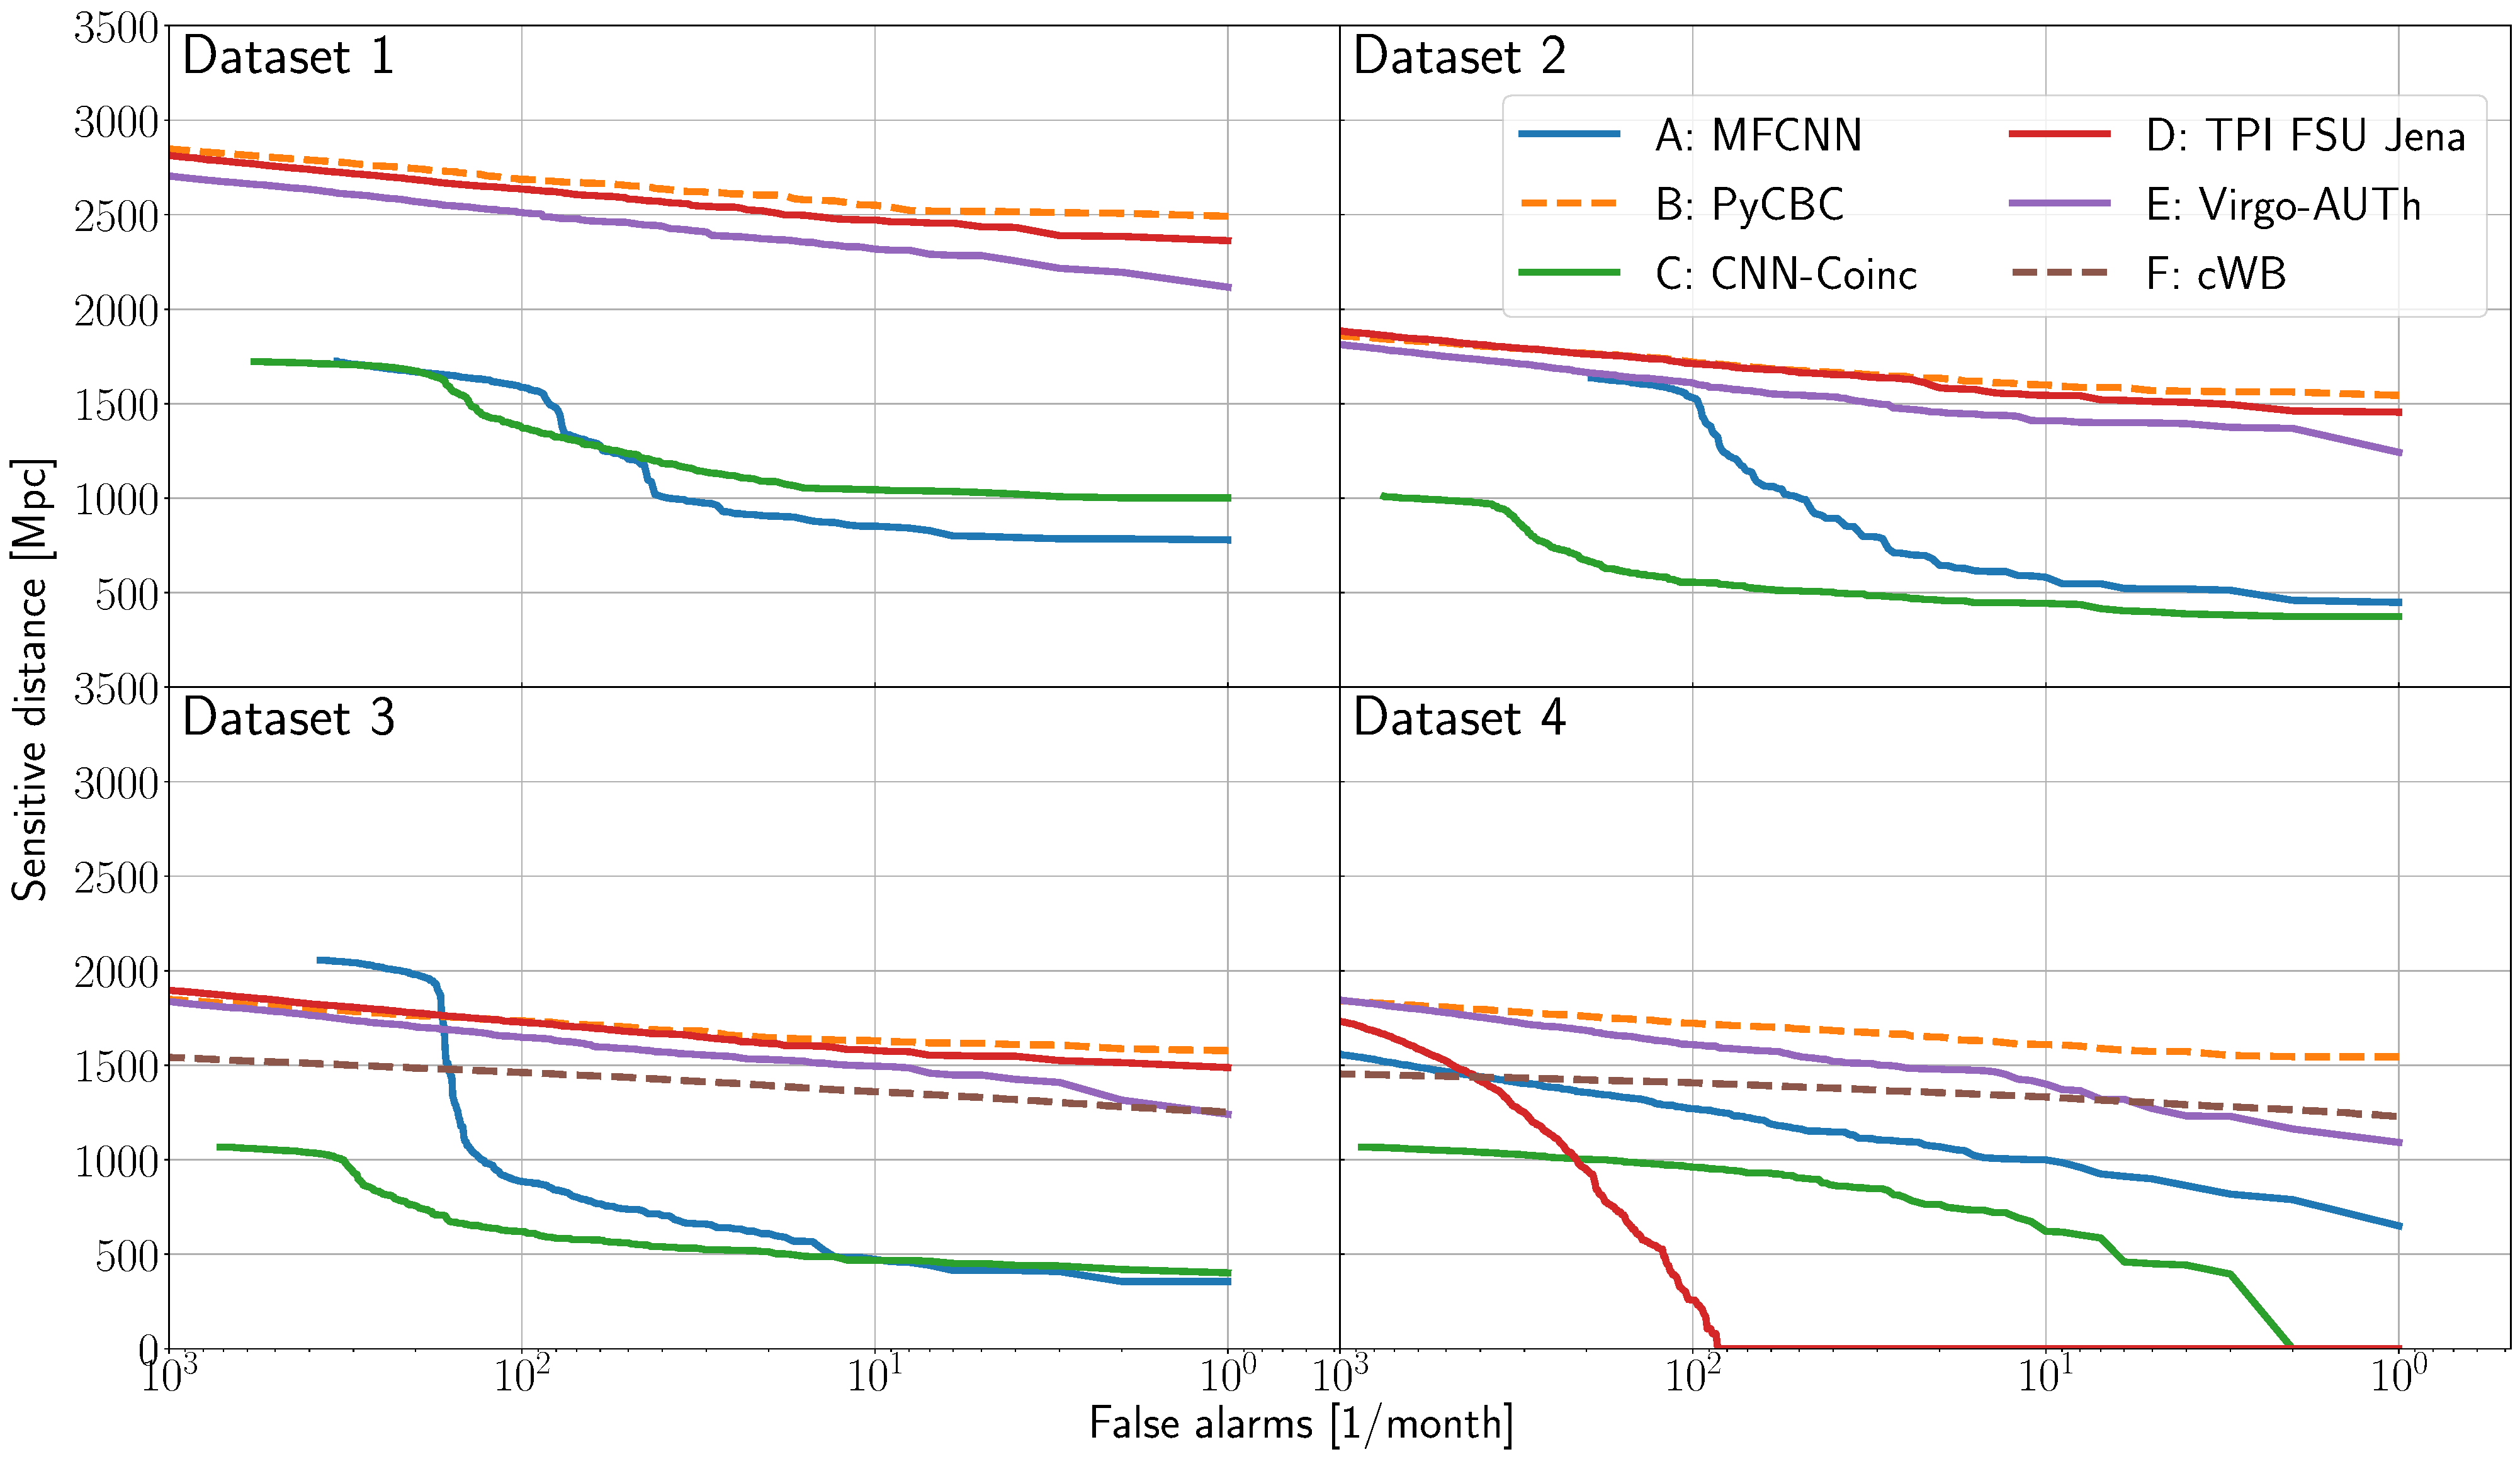
\includegraphics[width=0.98\textwidth]{chapters/mdc/images/sens.pdf}
    \caption[Sensitive distances]{The sensitive distances of all submissions and all four datasets as functions of the \acrshort{far}. Submissions that made use of a machine learning algorithm at their core are shown with solid lines, others with dashed lines. The \acrshort{far} was calculated on a background set that does not contain any injections.}
    \label{fig:mlgwsc_sens}
\end{figure*}
\begin{table*}[]
    \centering
    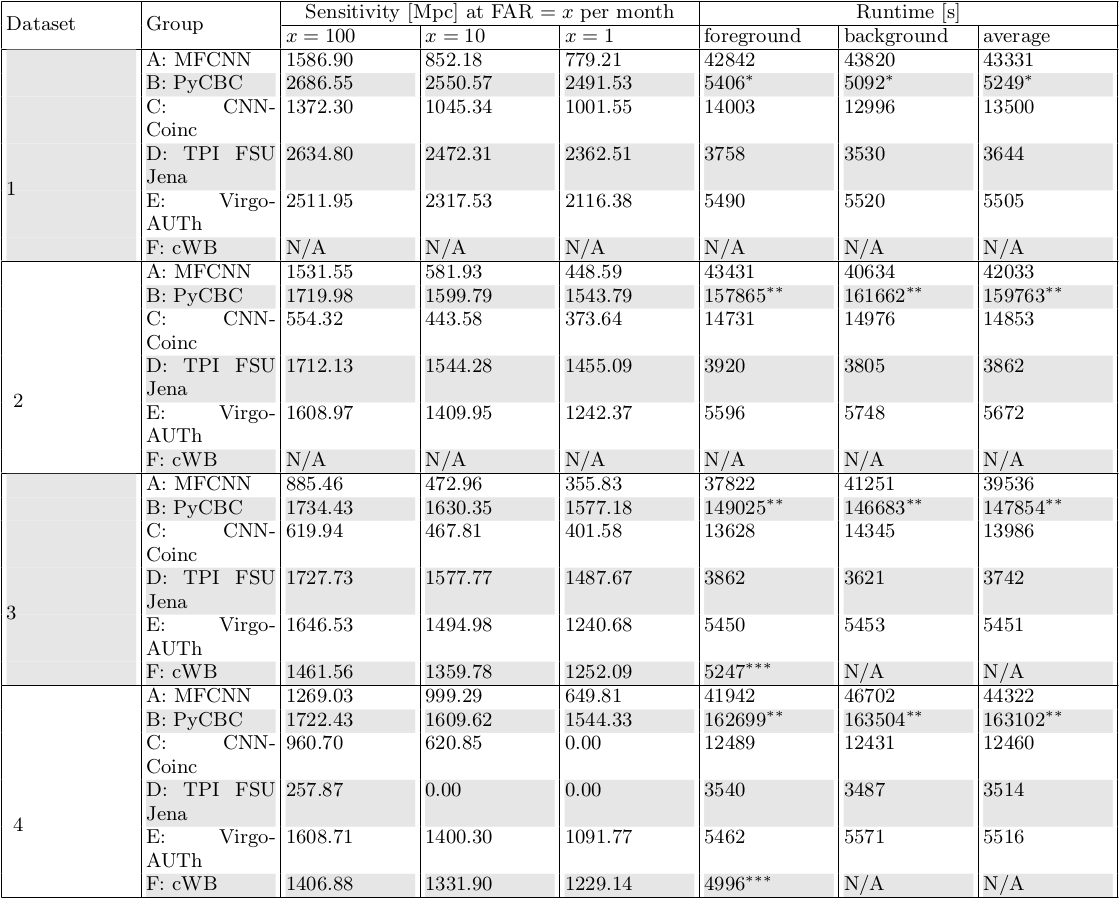
\includegraphics[width=\textwidth]{chapters/mdc/images/long_table}
    \caption[Results]{A summary of the analysis results for all submissions and all datasets. The columns labeled ``Sensitivity'' give the values for the sensitive distance at the three \acrshort{far}s $10^2$ per month, $10^1$ per month, and $10^0$ per month rounded to the second decimal place. The values lie on the lines in \autoref{fig:mlgwsc_sens}. The columns labeled ``Runtime'' list the time for evaluation of the foreground and background set in seconds, respectively. The runtime column labeled ``average'' lists the mean time obtained from evaluating the foreground and background data. Entries labeled ``N/A'' are not available, because they were not measured. The \pycbc times labeled with $^\ast$ are only approximations. The analysis did not run on the challenge hardware but made use of a compute cluster. Shown times are the result of scaling the computational costs to 16 CPU cores. The \pycbc times labeled with $^{\ast\ast}$ are approximations obtained in the same manner as the approximations labeled with $^\ast$, but make use of a larger filter bank. The times of the \cwb group marked with $^{\ast\ast\ast}$ are approximations derived from dividing the CPU core-seconds reported by the search by $16$ to normalize it to the challenge hardware.}
    \label{tab:res}
\end{table*}

We find that the machine learning algorithms from the \jena group presented in \autoref{sec:submission-jena} and the \virgo group presented in \autoref{sec:submission-auth} are very close in sensitivity for datasets 1, 2, and 3. The submission from the \jena group reaches a slightly higher sensitive distance at all \acrshort{far}s for all of these three datasets. However, the \virgo submission retains $\geq 90\%$ of the sensitive distance achieved by the \jena submissions for \acrshort{far}s $\geq2$ per month. At lower \acrshort{far}s the gap widens but the individual sensitivities carry large uncertainties due to low number statistics. For higher \acrshort{far}s this gap narrows to a separation of roughly $4\%$ at a \acrshort{far} of $1000$ per month. We suspect that the difference between the two approaches is on the order that could be explained by different initializations of the training procedure.

On dataset 4 the submission from the \virgo group manages to maintain a stable sensitivity for the full range of tested \acrshort{far}s. The submission from \jena, on the other hand, is dominated by background triggers and seemingly struggles to adjust to the non-Gaussian noise characteristics. For high \acrshort{far}s the sensitivity is on a similar scale as the submission from the \virgo group and as was observed on previous datasets, backing up the hypothesis that rejecting background triggers is the main problem. This is surprising, as both algorithms were optimized on dataset 4 but performed similarly only on datasets 1 to 3. One reason for this result may be the neural network architectures used by the different groups. The \virgo group uses a very deep ResNet that may be better suited to represent non-Gaussian noise artifacts. The architecture from the \jena group is a more straightforward convolutional architecture that may be limited in its ability to learn appropriate parameters.

The algorithms from the \mfcnn group presented in \autoref{sec:submission-mfcnn} and the \cnn group presented in \autoref{sec:submission-cnn} also show similarities in sensitivity. Both are significantly less sensitive than the leading machine learning submission on all datasets. For datasets 1, 2, and 3, the \mfcnn contribution achieves $32.5\%$, $30.8\%$, and $23.5\%$ of the sensitive distances of the leading machine learning contribution, respectively. The \cnn submission reaches $42\%$, $25.5\%$, and $27\%$ of the sensitivity of the leading machine learning contribution at the point of farthest separation. For dataset 4 the submission from the \mfcnn and \cnn groups do comparatively better. They retain $\geq 68\%$ and $\geq 50\%$ of the sensitive distance of the leading machine learning submission down to a \acrshort{far} of $10$ per month, respectively. At a \acrshort{far} of $1$ per month the \cnn submission does not detect any signals, whereas the \mfcnn still retains $60\%$ of the sensitivity of the leading machine learning contribution.

On the first three datasets one can observe a steep gradient of the sensitivity curves at varying \acrshort{far}s for the \mfcnn and \cnn submissions. At even higher \acrshort{far}s the curves level off again and return to a similar slope observed at low \acrshort{far}s. The sudden increase leads to the \mfcnn submission being more sensitive than the modeled \pycbc search by up to $15\%$ on dataset 3 for \acrshort{far}s $> 200$ per month. This behavior is not present in any of the other submissions and we were not able to find a clear explanation. However, we observe that both algorithms have different trigger rates on the foreground and background set. If the background is estimated from the foreground data only, the sensitivity of both algorithms drops sharply. All other algorithms are robust to this change. We show these sensitivity curves in \autoref{fig:sens_fg}. However, it was communicated to the groups before submission that sensitivities would be calculated using both the foreground and background data. For this reason, we do not discuss \autoref{fig:sens_fg} any further but would like to encourage possible future mock data challenges to drop the background set.

For all datasets we compare the leading machine learning submission to the submission from \pycbc presented in \autoref{sec:submission-pycbc}. We also compare it to the submission from \cwb presented in \autoref{sec:submission-cwb} for datasets 3 and 4. These two are traditional, state-of-the-art search algorithms that have already been used successfully in past observation runs~\cite{LIGOScientific:2016fbo, LIGOScientific:2016aoc, LIGOScientific:2021djp}.

For dataset 1 we find that the machine learning search is able to achieve between $94\%$ and $99\%$ of the sensitivity obtained with PyCBC. These results are remarkably close and improve significantly on the findings from \cite{Schafer:2021cml}, which targeted a very similar dataset. However, the gap between the machine learning detection algorithm and the \pycbc search widens for lower \acrshort{far}s. Therefore, we expect that the \pycbc contribution will be able to attribute a substantially higher significance to many events. This is amplified by the ability of \pycbc to trivially increase the amount of data that can be used for background estimation by introducing time-slides between detectors~\cite{Usman:2015kfa, Schafer:2021cml}.

For dataset 2 the leading machine learning contribution gets even closer to the traditional algorithm from the \pycbc group. At low \acrshort{far}s $\leq 20$ per month it retains $\geq 93.5\%$ of the sensitivity achieved by the \pycbc submission. For high \acrshort{far}s $\geq 200$ per month it even manages to outperform the \pycbc submission and is up to $1.5\%$ more sensitive.

From dataset 2 to dataset 3 all submissions experience a slight increase of the measured sensitive distance. This may be surprising at first but can be explained by the distribution of the effective spin. For dataset 3 the spin orientations are distributed isotropically, which causes the average effective spin to be smaller than in dataset 2. This leads to few systems with large effective spin. The \pycbc search gains up to $3\%$ in sensitivity at low \acrshort{far}s, although it loses about $1\%$ in sensitivity at high \acrshort{far}s. A similar change can be observed in the submission from \jena. Since both the leading machine learning contribution and the \pycbc search gain similar amounts of sensitivity from dataset 2 to dataset 3 the comparison between the two does not change substantially. The submission from the \jena group is now up to $2.5\%$ more sensitive at high \acrshort{far}s and still about $6\%$ less sensitive at low \acrshort{far}s. The \virgo, the \mfcnn, and the \cnn submissions increase their sensitive distance by a larger fraction, suggesting that they benefit more from the signal population being closer to the distribution of signals in their training set. Dataset 3 is also the first dataset for which results from the \cwb search are available. We find that \cwb retains $\geq 80\%$ of the sensitive distance obtained by \pycbc over all tested \acrshort{far}s. Subsequently the leading machine learning submission achieves a sensitive distance greater by $15\%$ to $23\%$ over the range of tested \acrshort{far}s.

For dataset 4 the leading machine learning contribution now comes from the \virgo group. Compared to \pycbc their algorithm retains $\geq 87\%$ of the sensitivity down to a \acrshort{far} of $10$ per month. For smaller \acrshort{far}s the sensitivity gap widens quickly. At a \acrshort{far} of $1$ per month the machine learning search achieves $70\%$ of the sensitivity of \pycbc. The \cwb submission evolves similarly to \pycbc and retains $\geq 79\%$ of the sensitive distance. At high \acrshort{far}s the leading machine learning search manages a sensitive distance up to $27\%$ larger than that of \cwb. For low \acrshort{far}s the sensitive distance falls off quicker than that of \cwb. At a \acrshort{far} of $1$ per month the \cwb search is $12.5\%$ more sensitive than the \virgo submission. For lower \acrshort{far}s we expect this difference to become larger, as the production level search algorithms are tuned for lower \acrshort{far}s than tested in this work. In comparison to the sensitivity difference on dataset 3 the machine learning submission from \virgo does not retain as much sensitivity on real noise as the \pycbc or \cwb submissions.

The results on dataset 1 demonstrate that machine learning detection algorithms are already capable of rivaling traditional search algorithms for simulated data at \acrshort{far}s $\geq 1$ per month. A previous study~\cite{Schafer:2021cml} had identified the capability of machine learning searches to build an internal representation of the signal morphology as the main problem to achieve comparable sensitivities to traditional algorithms. Such a signal representation would allow the algorithms to compare detections in multiple detectors and require them to be consistent. The two leading machine learning algorithms in this challenge seem to have overcome this limitation, at least for high \acrshort{far} detections.

For dataset 2 we expected machine learning searches to decline in sensitivity more strongly than traditional searches. This expectation was provoked by the short duration of data that is processed by most machine learning searches at each step. As the signals injected into dataset 2 are of longer duration than those used in dataset 1, the machine learning algorithms inherently lose some amount of sensitivity due to considering only small parts of the signal. We estimate this loss to account for at most a $1\%$ difference in sensitivity. However, we observe the opposite effect for the two leading machine learning algorithms, which get even closer in sensitivity to the \pycbc submission compared to dataset 1. This may be caused by the distribution of signals in the training data used for the machine learning algorithms. Since both algorithms optimized for dataset 4, most signals in the training data will have non-zero spin. Therefore, the challenge set for dataset 2 is closer in nature to the training data, which may have introduced a bias that leads to higher sensitivities for spinning systems or in other words a slightly reduced sensitivity to non-spinning systems.

Dataset 3 was intended to test if machine learning searches are capable of outperforming traditional algorithms for precessing systems and signals carrying higher order mode information. We do not find substantial evidence in support of this hypothesis from the sensitivity curves. However, the challenge set 3 contains only very few signals with strong evidence for precession and higher order modes, as most signals are still relatively short. The impact on the overall sensitivity from these signals is, therefore, minor. Surprisingly, the leading machine learning search is still on par with \pycbc and manages to be significantly more sensitive even at the lowest tested \acrshort{far}s than the unmodeled \cwb search. It must be noted that the \cwb submission was not optimized for the parameter space used in this challenge. We, thus, expect this gap to narrow if more effort were to be used to tune the \cwb pipeline.

The change in the relative difference in sensitivity between the \pycbc submission and the leading machine learning contribution, as well as the change in difference to the \cwb submission, from dataset 3 to dataset 4 suggests that many machine learning algorithms currently used by the community are not yet capable of treating real noise as well as sophisticated traditional algorithms. We suspect that one major factor may be non-Gaussian noise artifacts that are misclassified as signals by machine learning algorithms, while the traditional searches excise them from the data or reject them on other bases. Another reason may be the non-stationary character of the noise that may lead to different sensitivities at different times. However, this would have also been a factor in dataset 3, where the \acrshort{psd}s used to simulate the noise change over the duration of the challenge set. However, since the leading machine learning search does retain sensitivity at all \acrshort{far}s it must have learned to reject most non-Gaussian noise artifacts, which is in line with expectations from studies carried out at higher \acrshort{far}s~\cite{George:2017pmj, Gebhard:2019ldz, Krastev:2020skk, Wei:2020sfz}.


\subsection{Found and missed injections}
We generate found-missed plots for all submissions and show a few selected ones. The ones not included in this paper can be found in the associated data release~\cite{github}. These plots highlight specific areas in parameter space where the machine learning searches are already competitive and those where more work is required. Specifically, we provide plots for chirp mass $M_c$ versus decisive effective chirp-distance $D_{c,\text{eff}}$, $\tau_0$ versus mass ratio $q$, and the effective precession spin $\chi_p$~\cite{Schmidt:2014iyl} versus inclination with respect to the line of sight $\theta_{jn}$. To first order $\tau_0$ is the time to merger from the lower frequency cutoff of the waveform~\cite{Cokelaer:2007kx, Maggiore:2008aaa}. The decisive effective chirp-distance is a measure for how strong the signal can be observed in the detector that has the worse sensitivity due to source location and orientation. The effective chirp-distance is the chirp-distance at which a source with the same intrinsic parameters and sky location but an optimal orientation would have been observed from at the same amplitude as the injected signal. The decisive effective chirp-distance is then the larger of the two effective chirp-distances from the two detectors. Therefore, the $M_c/D_{c,\text{eff}}$ plot informs about the ability to detect signals as a function of the \acrshort{snr} in the detector that is less sensitive to the signal. We also include information on the ranking statistic like quantity returned for each detected event, to highlight how strongly it is correlated to the \acrshort{snr}. The $\tau_0$ versus $q$ plot highlights how well long and short duration signals are recovered. It also gives information on the mass ratio, which is an important parameter for the strength of precession effects. The main plot used to determine the impact precession effects and higher order modes have on the detectability of signals is the $\chi_p$ versus $\theta_{jn}$ plot.

In \autoref{fig:ds1md} we show the found injections from dataset 1 in the $M_c$-$D_{c,\text{eff}}$-plane for the \pycbc and \jena submissions, respectively. Both plots clearly show that closer injections are generally attributed a higher confidence to be a real signal. This indicates that the ranking statistic like quantities for both algorithms are actually correlated with the signal strength. Similar correlations can be observed for all submissions. Furthermore, all signals with large $D_{c,\text{eff}}$ are missed by both searches, showing that sensitivity estimates are not limited by the injected population. From \autoref{fig:ds1md} we find that the chirp mass distribution from the \jena submission favors chirp masses in the region $M_c\in[20, 35]$, which is not true for the \pycbc submission. We attribute this bias to the training set, which contained signals drawn from the distributions used for dataset 3 and 4. The probability distribution of the chirp mass for these sets is shaped such that about $51\%$ of signals are being drawn from the mass range \SI{20}{M_\odot} to \SI{35}{M_\odot}. A similar bias is not so evident for the other machine learning submissions but may be masked by other effects. The \pycbc submission uses a uniform prior on the chirp mass and thus avoids this bias.

In \autoref{fig:ds2tq} we compare the found injections from dataset 2 in the $\tau_0$-$q$-plane for the \pycbc and \jena submissions. The plots show that the two searches are competitive in the comparable mass region and identify similar signals. The main difference between the two searches can be observed in the $\tau_0$ distribution of found signals. Most of the signals with large values for $\tau_0$, i.e. long duration signals, are missed by the \jena submission. These crucially include many signals that the \pycbc submission identifies with relatively high confidence. Therefore, the short duration of the input windows used by the \jena submission still seem to be a limiting factor for the sensitivity. This limitation will likely be more severe if longer duration signals from sources like \acrshort{bns} or \acrshort{nsbh} systems were considered.

In \autoref{fig:ds3chitheta} we compare the $\theta_{jn}$ and $\chi_p$ values of the injections from dataset 3 that are found by one algorithm but missed by the other. The two algorithms come from the \pycbc group and the \jena group. If either algorithm adapted better to signals with strong precession or higher order modes content, we would expect to see a clustering from that search in the scatter plot. However, we do not observe this clustering, which backs up our observation from the sensitivity curves that the machine learning algorithm from the \jena group has not learned a better representation of precessing systems or signals with higher order mode content than the modeled \pycbc search, which only includes non-precessing signals in its template bank. However, the amount of impact precession or higher order modes have on the detectability of short duration signals used in this study are small. A real test of this hypothesis would require the analysis of long duration signals.


\subsection{Runtimes}
All runtimes in this section are given in terms of wall-clock times obtained on equivalent hardware, which is listed in \autoref{tab:hardware}. The  runtimes are largely independent of the dataset for all submissions. We, therefore, discuss them only in summary. An overview of the times can be found in \autoref{tab:res}. They were measured by applying each algorithm to the foreground and background of each challenge set. We report the time between the algorithm call and it returning. To avoid bottlenecks, all files were transferred to the local storage of the individual compute nodes before calling the algorithm. The output was also written to said local storage and transferred back only after the algorithm returned. It should be noted that the runtimes are heavily dependent on the amount of optimization of the algorithms. The main objective for this challenge was the sensitivity and not the runtime.

The \pycbc and \cwb submissions are exceptions as their runtimes were not measured on the same hardware. Instead they were run on compute clusters making heavy use of parallelized work over multiple CPUs. The times reported here are approximations by normalizing the compute time to 16 CPU cores available in the compute nodes used for this challenge. Furthermore, for the evaluation of dataset 1 \pycbc used a different template bank than those for dataset 2 to 4 was used. This bank was substantially smaller, resulting in faster evaluation. \cwb times were reported to us only on the foreground data in CPU core seconds.

We find that of the machine learning algorithms the submission from the \jena group is the fastest, evaluating an entire month of archival data in about \SI{1}{\hour}. It utilizes a single GPU when evaluating the network. The second fastest algorithm is the submission from the \virgo group. It evaluates a month of data in \SI{1.5}{\hour} on a single GPU and is thus about $50\%$ slower than the fastest algorithm. Notably, the two fastest algorithms are also the two most sensitive machine learning searches. The algorithm from the \cnn group requires almost \SI{4}{\hour} on a single GPU to evaluate the same amount of data but is significantly less sensitive. However, none of these algorithms are limited by the GPU performance. The differences in execution time can be mainly attributed to the difference in optimization of the pre-processing steps. The submission from the \mfcnn group on the other hand does not apply any pre-processing directly. They instead use a neural network to carry out this computation. They operate on all 8 available GPUs and manage to evaluate the month of data in \SI[parse-numbers=false]{\approx 11.5}{\hour}.

For dataset 1 the \pycbc submission has a runtime comparable to that of the submission from the \virgo group. On all other datasets it requires roughly \SI{43}{\hour} to evaluate the month of data. The large difference in runtime between the datasets is caused by the smaller template bank that is used only for dataset 1. Contrary to the machine learning algorithms, the \pycbc submission did not utilize GPUs and ran on CPUs only. However, \pycbc is a production level search pipeline and as such has been optimized to run on CPUs. It is not limited by the pre-processing but rather by the matched filter operation. It should be noted that \pycbc is still the most sensitive search presented here and gains in computational efficiency could be obtained by reducing the number of templates. This would effectively trade off search sensitivity for lower computational cost.

The \pycbc submission is implemented on the CPU as a GPU implementation is inherently more difficult to optimize. GPUs, on the other hand, are usually far more efficient from a cost to performance and energy to performance standpoint~\cite{Dhurkunde:2021csz}. One advantage of machine learning algorithms is that they make use of well optimized libraries such as PyTorch~\cite{Paszke:2019aaa} or TensorFlow~\cite{Abadi:2015aaa} that utilize GPUs for their computations. This makes the implementation of search algorithms on GPUs relatively straightforward and allows researchers to focus on optimizing the sensitivity of their algorithm rather than having to spend time on optimizing the algorithmic implementation. 

The runtimes in this challenge are measured under the assumption that the lowest required \acrshort{far} is $1$ per month. In a real search lower \acrshort{far}s are beneficial especially for rare signals. Therefore, most traditional searches are tuned to be most sensitive at \acrshort{far}s well below the level tested in this challenge. \pycbc for instance can extend its background by introducing time-slides~\cite{Usman:2015kfa}, thereby potentially lowering the \acrshort{far}s of detected events. This process is a trivial operation that requires a fraction of the computational cost of the actual filtering stage. If machine learning algorithms are not specifically designed to allow for a similar approach, lowering the \acrshort{far}s of detections requires multiple complete re-evaluations of the time-shifted data. This would in turn lead to a linear increase in the computational cost, i.e. lowering the potential \acrshort{far} of an event by an order of magnitude would lead to an order of magnitude increase in the computational cost.


\section{Conclusions}\label{sec:mlgwsc_conclusions}
In this paper we have presented the results of the first Machine Learning Gravitational Wave Search Mock Data Challenge (MLGWSC-1). The study compiled curves showing the sensitive distances from $4$ different machine learning submissions and compared them to $2$ state-of-the-art traditional search algorithms; the modeled PyCBC~\cite{Usman:2015kfa} pipeline and the unmodeled coherent wave burst search~\cite{Klimenko:2015ypf,Klimenko:2004qh}. We established a common dataset and means for evaluation. We hope that other researchers will continue to make use of the resources presented in this work to allow for quantitative comparisons between different machine learning approaches and to traditional filtering techniques. As research continues and machine learning search algorithms become more sensitive, we want to motivate other groups to host new challenges, focusing on other parts of parameter space or targeting different observing strategies.

The key observations of this challenge are:
\begin{enumerate}
    \item Machine learning search algorithms are competitive in sensitivity compared to state-of-the-art searches on simulated data and the limited parameter space explored in this challenge.
    \item Most of the tested machine learning algorithms struggle to effectively handle real noise, which is contaminated with non-Gaussian noise artifacts.
    \item Traditional search algorithms are capable of detecting signals at lower \acrshort{far}s, thus making detections more confident.
    \item The tested machine learning searches struggle to identify long duration signals.
\end{enumerate}
Therefore, the main challenges for current machine learning searches are the operation on real noise, the confidence in detections due to comparatively high \acrshort{far}s, and the detection of long duration signals. The last of those three is a major hurdle to confidently detect signals from \acrshort{bns} and \acrshort{nsbh} systems. Improvements in any of these fields would be beneficial. Specifically, we identify the following key research areas:
\begin{enumerate}
    \item Improve the ability to compare signal parameters, or representations thereof, between detectors to check for consistency and reject noise artifacts.
    \item Improve the ability to calculate large amounts of background, for instance by designing algorithms that can trivially evaluate time-slides of the input data.
    \item Increase the duration of data that is processed by machine learning algorithms to enable the detection of long duration signals.
\end{enumerate}

This challenge shows the potential of machine learning algorithms to act as \acrshort{gw} detection pipelines. We have shown that these algorithms are competitive in a realistic scenario to state-of-the-art searches today. They operate at low computational cost and allow for a trivial implementation of the algorithms on highly efficient GPUs, rather than relying on CPUs. We believe that this work justifies more research on this topic, especially in areas where machine learning may have a tangible impact on the rapid identification of \acrshort{gw}s.

However, we do acknowledge that the research carried out here operates on a limited parameter space. Moreover, the targeted parameter space is not the computationally expensive part of the search space of traditional searches. About $1\%$ of the total size of the template bank used in \cite{Nitz:2021zwj} is dedicated to the area this study searches. To have the greatest impact on real searches machine learning algorithms need to be extended to target either the low mass region, where signals are long and the computational cost of matched filtering rises rapidly, or the high mass region where signals and noise artifacts are difficult to distinguish.

We also want to mention that we did not receive a submission utilizing one of the most promising neural network architectures for \acrshort{gw} detection of the recent past. A WaveNet based architecture, that uses dilated convolutions, has been reported to do well for this kind of task~\cite{Gebhard:2019ldz, Schmitt:2019aaa, Wei:2020ztw}. We also did not receive submission based on many other neural network architectures that have been used in the past, such as autoencoders~\cite{Shen:2019ohi, Morawski:2021kxv, Moreno:2021fvp, Bacon:2022lsm}, inception networks~\cite{Dreissigacker:2020xfr, Schafer:2020kor}, or two dimensional convolutions that analyze time-frequency decompositions~\cite{Wei:2020sfz}. We hope that some of these approaches will be adopted to the requirements of this challenge and evaluated on the datasets presented here, to allow for a quantitative comparison.

Future mock data challenges could target longer duration signals, concentrating on \acrshort{bns} and \acrshort{nsbh} systems. These are potentially EM-bright and would, therefore, be of particular interest. Furthermore, these signals stem from regions of parameter space where traditional searches are computationally expensive to run. For even longer signals, sub-solar mass black holes could be targeted. Existing modeled searches in those regions make use of several million templates and are computationally limited~\cite{Nitz:2022ltl}. Another avenue may be very massive systems, which can be difficult to distinguish from noise artifacts. Finally, we recommend that future mock data challenges drop the notion of a foreground and background set and only provide data files containing injections. This would eliminate further sources of error and be more true to a realistic application, where no true \acrshort{gw}-free background exists.

\begin{figure*}
    \centering
    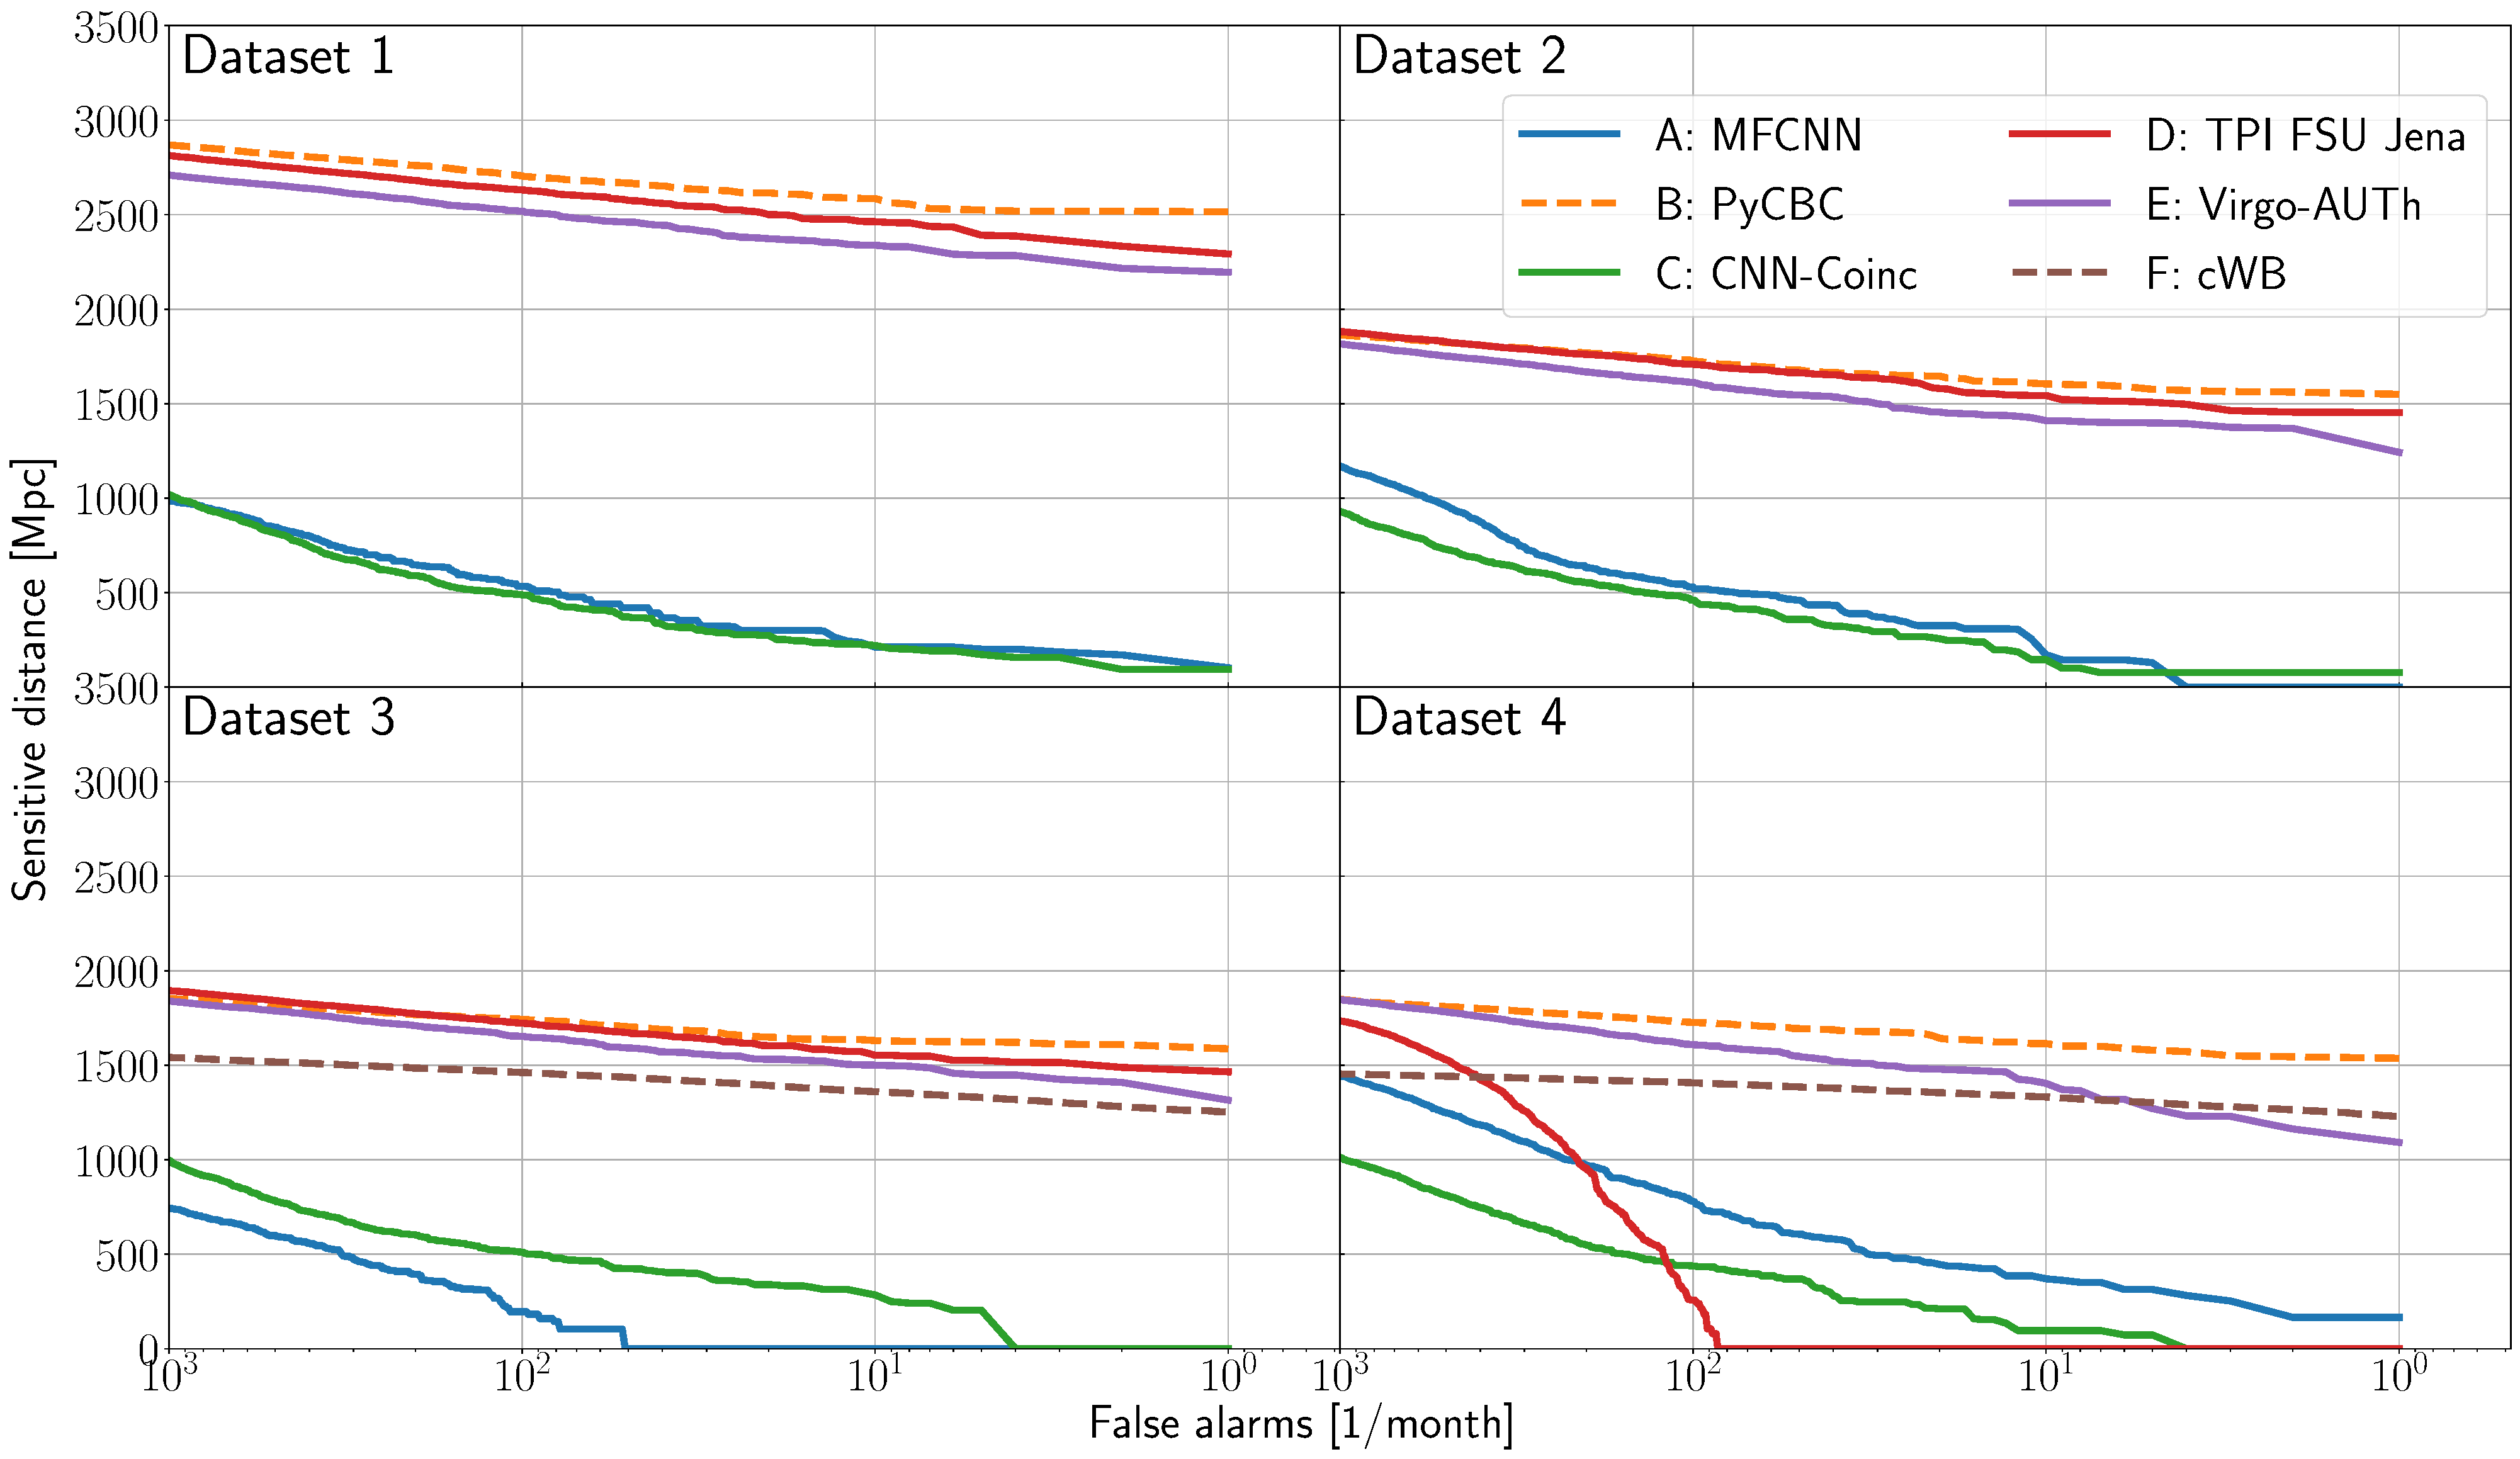
\includegraphics[width=0.98\textwidth]{chapters/mdc/images/sens_fg.pdf}
    \caption[Sensitive distance calculated on foreground]{The sensitive distances of all submissions and all four datasets as functions of the \acrshort{far}. The sensitive distances are calculated using only the data from the foreground file. The \acrshort{far} is determined from the false positives on that data. Submissions that made use of a machine learning algorithm at their core are shown with solid lines, others with dashed lines. This figure differs from \autoref{fig:mlgwsc_sens} as the algorithms from \mfcnn and \cnn behave differently on the foreground and the background.}
    \label{fig:sens_fg}
\end{figure*}

\begin{figure*}
    \centering
    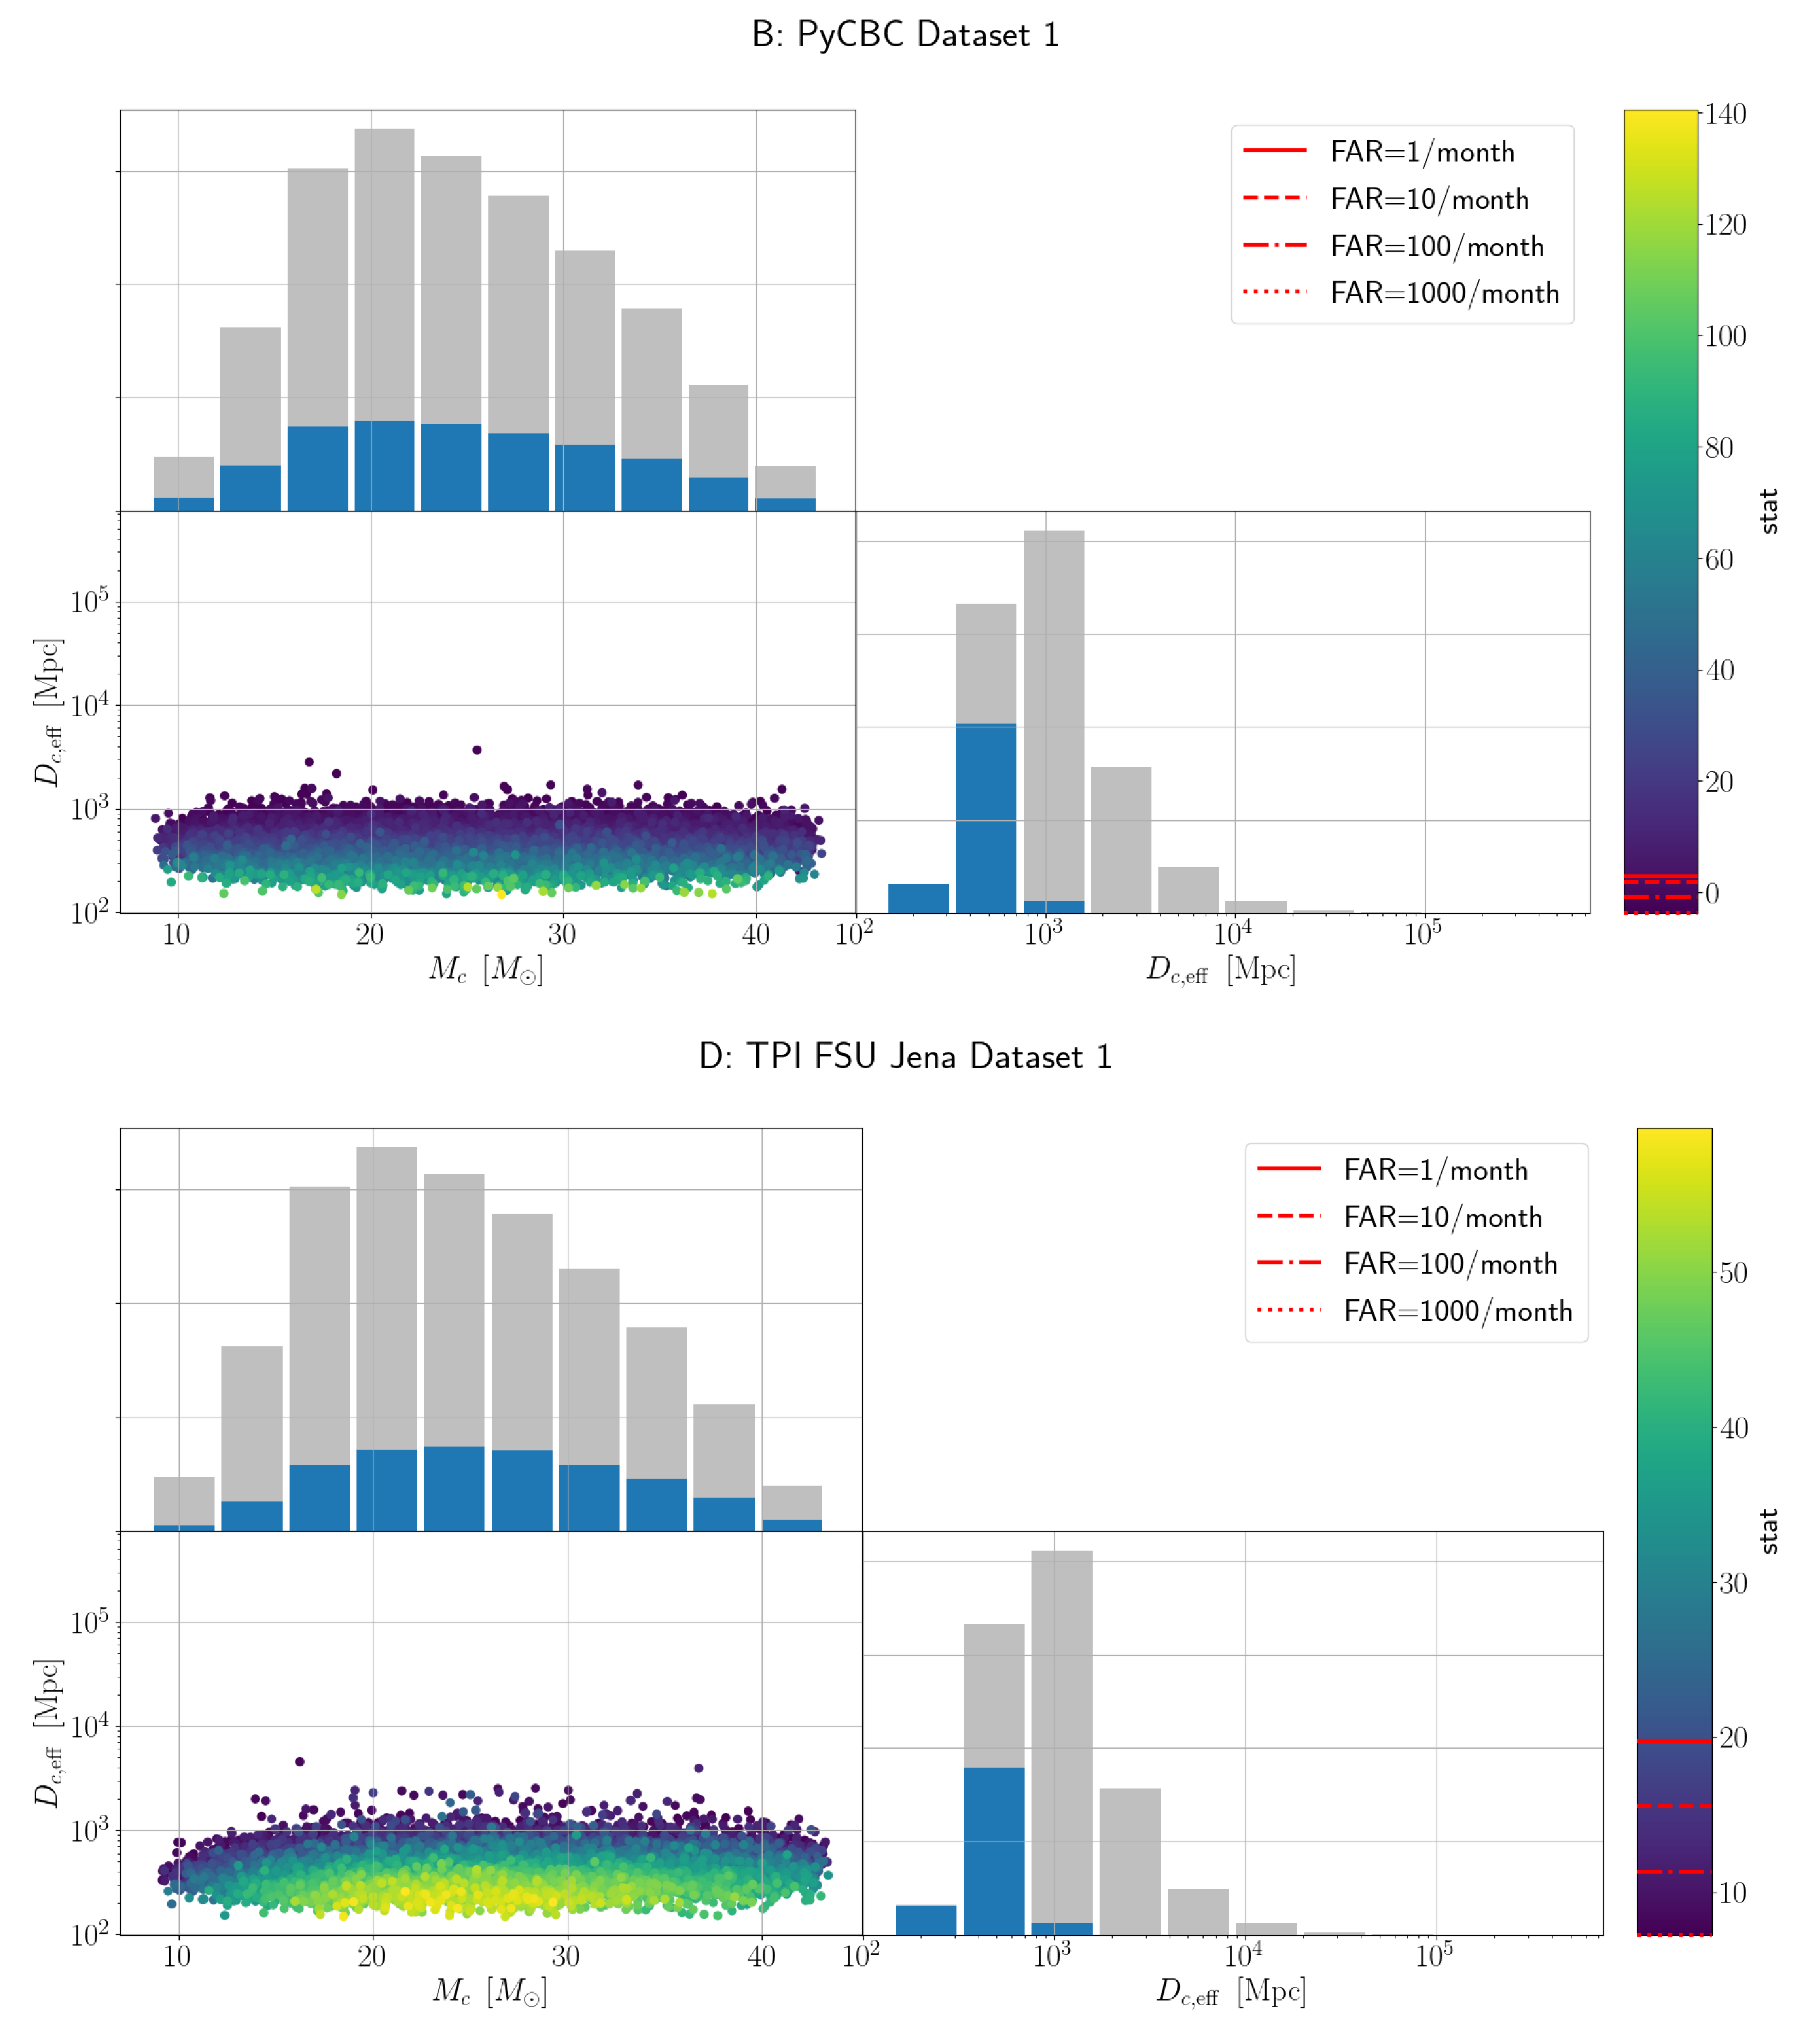
\includegraphics[width=0.9\textwidth]{chapters/mdc/images/mcd_found_ds1_pycbc_TPI_FSU_Jena.pdf}
    \caption[Found-missed chirp mass versus distance]{The injections from dataset 1 identified by the \pycbc and \jena submissions with a \acrshort{far} $\leq 10^3$ per month in the chirp mass $M_c$ versus decisive effective chirp-distance $D_{c,\text{eff}}$ plane. The blue bars in the histograms show the one dimensional marginal distributions of the found injections. The gray bars show the distribution of injected signals, including those missed by the search. The color shows the ``stat'' value attributed to the injection by the algorithm. The red lines in the colorbar highlight the thresholds on the ``stat'' to achieve different \acrshort{far}s.}
    \label{fig:ds1md}
\end{figure*}

\begin{figure*}
    \centering
    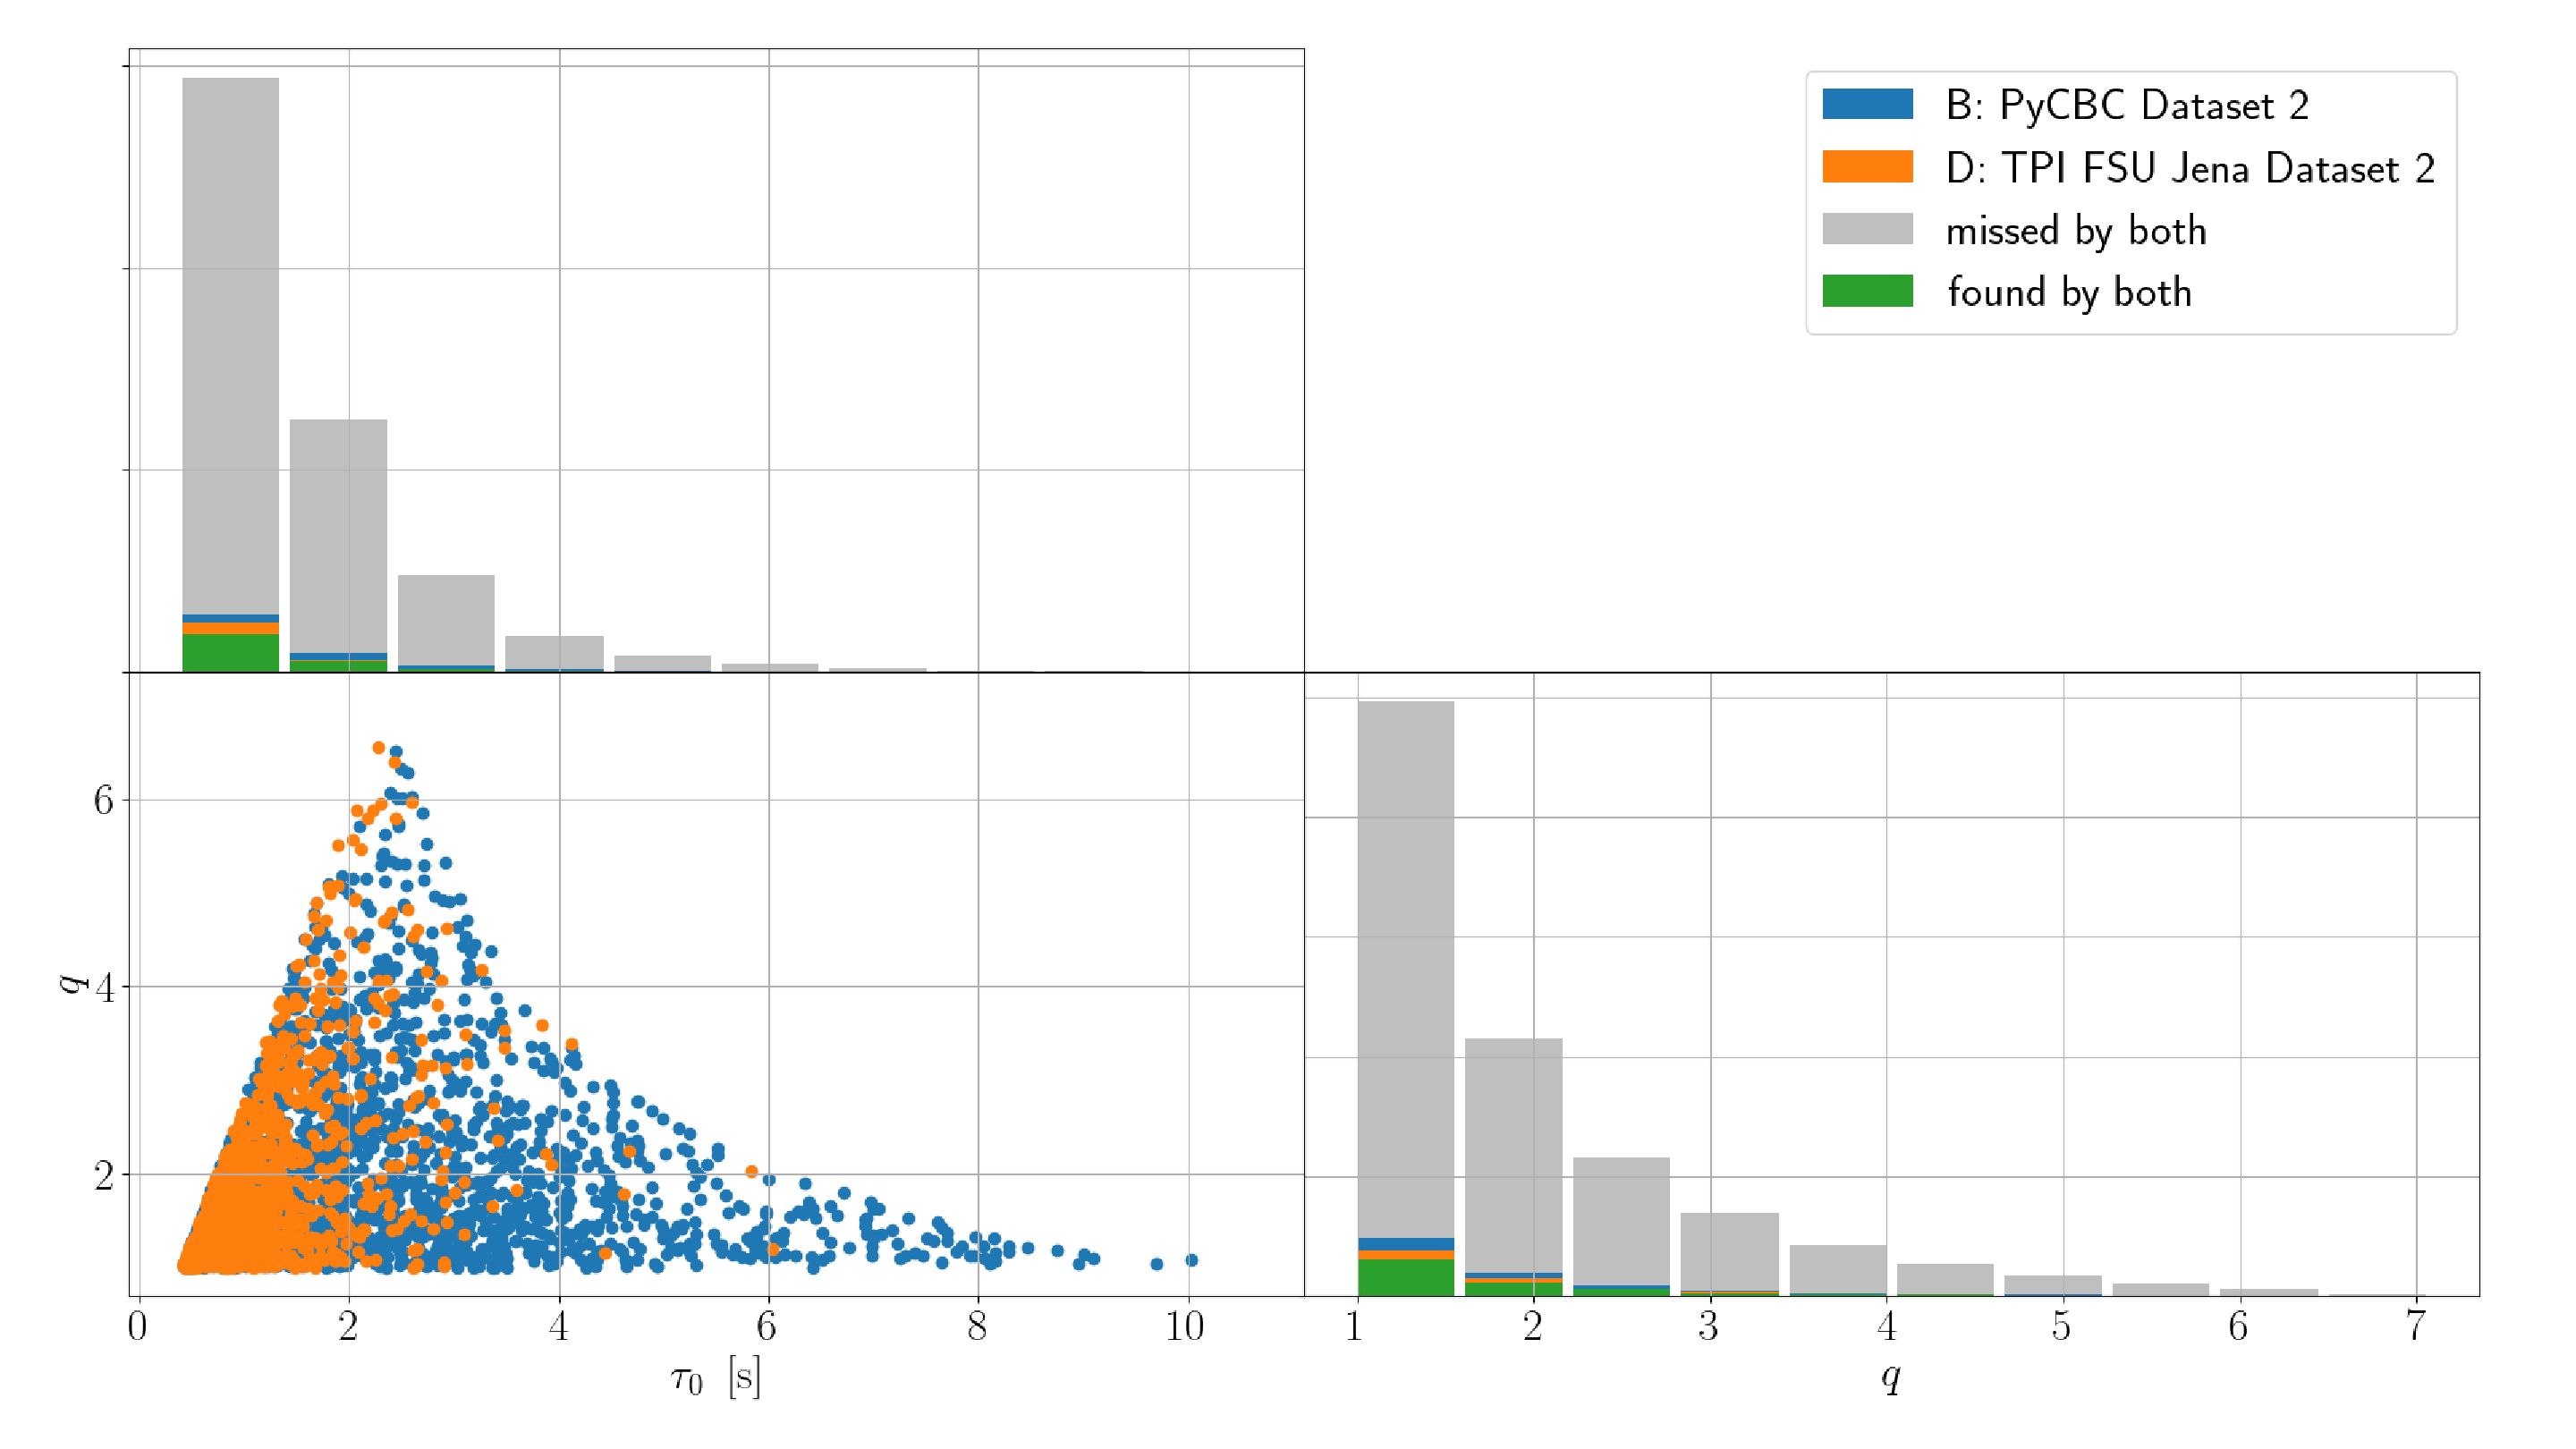
\includegraphics[width=0.9\textwidth]{chapters/mdc/images/tau0q_found_ds2_pycbc_TPI_FSU_Jena_plot.pdf}
    \caption[Found-missed template duration versus mass ratio]{The injections from dataset 2 identified by the \pycbc and \jena submissions with a \acrshort{far} $\leq 10^3$ per month in the signal duration $\tau_0$ versus mass ratio $q$ plane. The scatter plot shows injections that are found only by one of the two algorithms. Injections that are missed or found by both are only shown in the 1D marginal distributions.}
    \label{fig:ds2tq}
\end{figure*}
\begin{figure*}
    \centering
    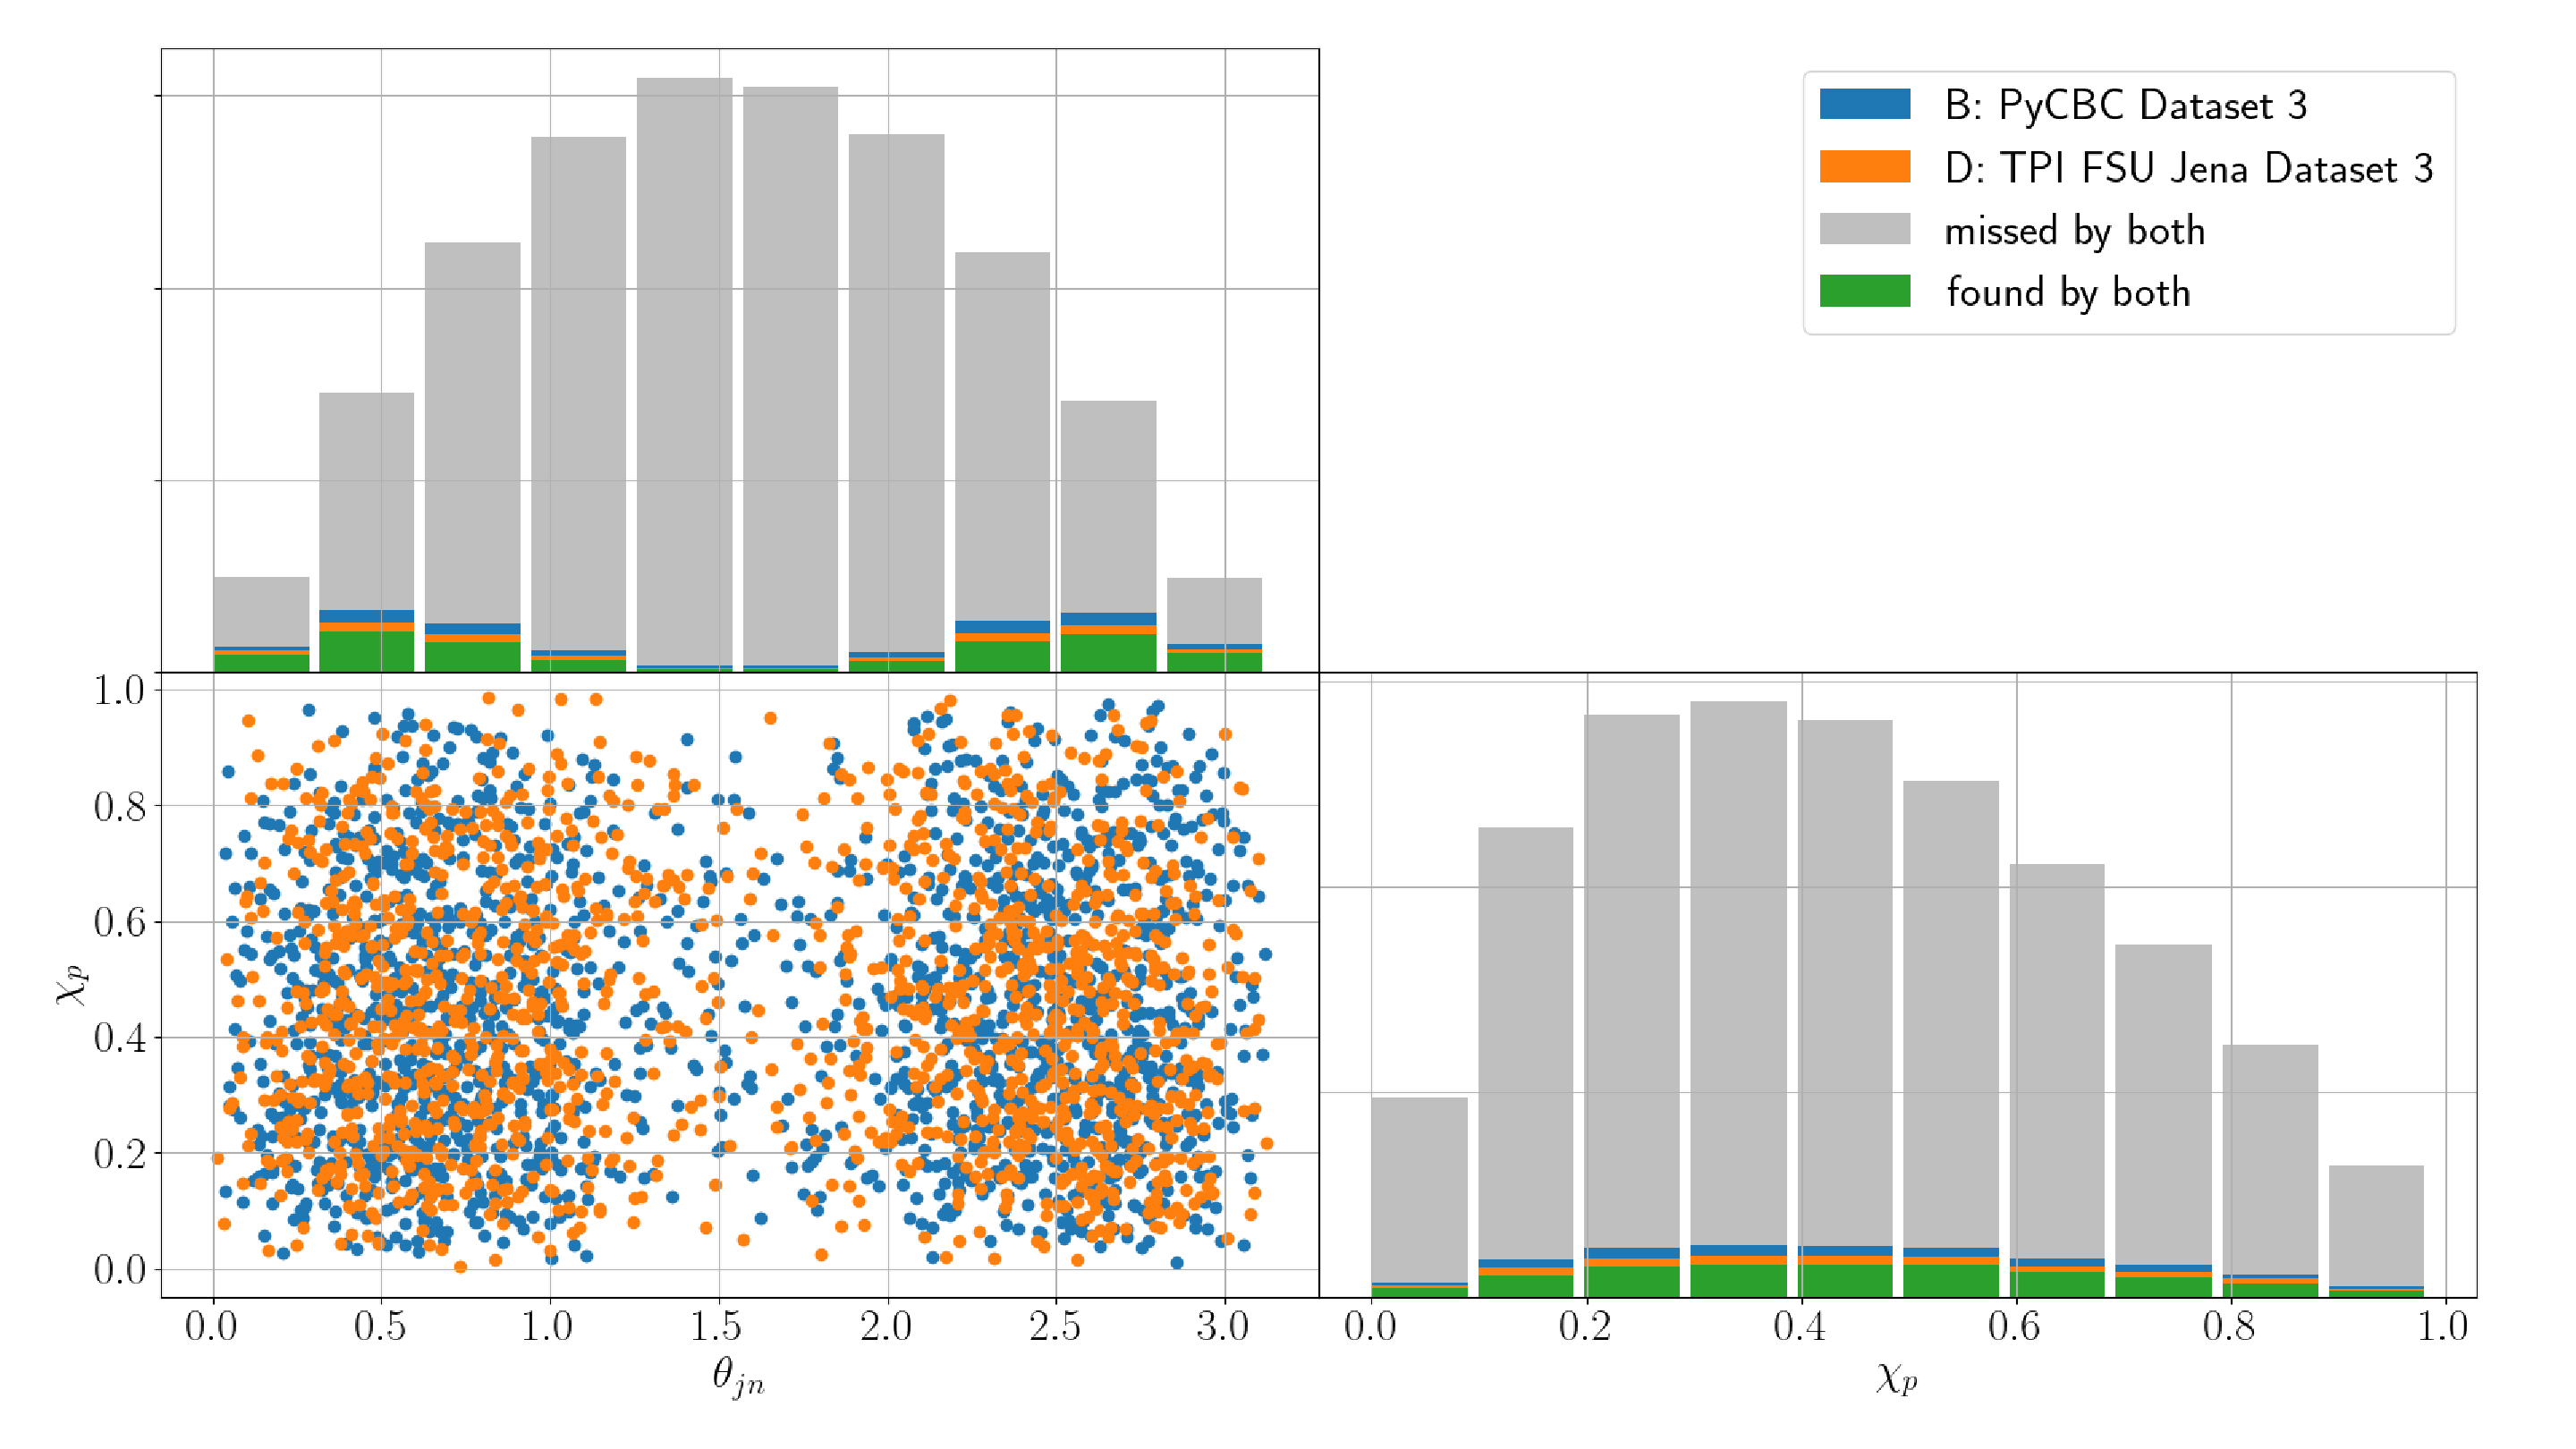
\includegraphics[width=0.9\textwidth]{chapters/mdc/images/chitheta_found_ds3_pycbc_TPI_FSU_Jena_plot.pdf}
    \caption[Found-missed effective precessing spin versus inclination]{The injections from dataset 3 identified by the \pycbc and \jena submissions with a \acrshort{far} $\leq 10^3$ per month in the inclination to spin axis $\theta_{jn}$ to $\chi_p$ plane. The scatter plot shows injections that are found only by one of the two algorithms. Injections that are missed or found by both are only shown in the 1D marginal distributions.}
    \label{fig:ds3chitheta}
\end{figure*}

\chapter{Internship at Bosch}\label{ch:bosch}
\minitoc
This chapter is somewhat independent from the rest of this thesis and summarizes a voluntary internship I did at Bosch Hildesheim, Germany. However, many advancements of \acrshort{ml} algorithms are developed in the industry and gaining an insight into their development environment is of great benefit to academic research. At Bosch I was part of the corporate research department focusing on unsupervised pre-training for computer vision (\acrshort{cv}) algorithms. Specifically, I was tasked with developing and testing self-supervised learning algorithms for object detection. Due to the independence of this chapter from the others, I will give a brief introduction to deep learning object detection algorithms and self-supervised pre-training algorithms before describing my research at Bosch.

During my 4 month internship I managed to test a framework originally presented in \cite{Wei:2021aaa} on data used internally at Bosch. Additionally, I experimented with multiple new and original ideas targeted at improving the original framework for the application at Bosch. My time at Bosch resulted in a total of 4 invention reports, one of which will be discussed below. The others are either too far from the core topics of this thesis or are not published yet.

\section{Basics of Object Detection}
Traditionally, \acrshort{cv} challenges like the \acrshort{ilsvrc} have mainly focused on image classification. The task in image classification is to provide a single label to an image. The famous ImageNet dataset contains more than $21\,000$ classes and 14 million images \cite{Fei-Fei:2022aaa}. In object detection the task is to locate and annotate objects in an image. So rather than providing one global label to the entire image, the algorithm needs to specify one or multiple regions and apply a label to every one of them.

Once a good image classifier is available, getting an accurate object detector is in principal not too difficult. Theoretically, the classifier can be applied to each possible sub-region of the image to get a label. When the image classifier is setup such that it has a garbage class that is used for all images that do not contain any object, it would be able to detect and correctly annotate objects in an image. However, this direct approach is prohibitively computationally expensive, due to the factorial growth of sub-regions with the dimensions of the input image. To reduce that cost at the price of accuracy, one can instead use pre-determined regions in the image and classify those. An alternative is to use a fast algorithm to filter out the majority of uninteresting regions with low accuracy and only classify the remaining ones.

Before an overview of the evolution of deep learning object detection algorithms is given, a few core concepts have to be defined. First, the output of an object detector in the context discussed here is a rectangular bounding box of an object, whose sides are parallel to the edges of the image. Each bounding box has to be classified into one of $N+1$ categories, where $N$ is the number of object classes. The last class is the background class, that represents non-detections. To quantify how well a predicted bounding box aligns with a labeled box, a quantity known as the \emph{intersection over union} (\acrshort{iou}) is commonly used. It is defined as the area of the intersection of two rectangles divided by the area of their union. To quantify the performance of an object detection algorithm, the most common metric is the \emph{mean average precision} (\acrshort{map}). The \emph{precision} is the number of true positive detections divided by the number of total detections. It measures how likely a detection is to be a true positive and depends on the requirement for how well a bounding box has to be aligned with the ground truth to be considered a true positive, i.e. it depends on \acrshort{iou} requirements. The \acrshort{iou} also influences how likely a ground truth is to be recovered by the algorithm. This is measured by the \emph{recall}, which is the number of true positives divided by the number of ground truths. Since both the precision as well as the recall are a function of the \acrshort{iou}, they can be plotted against one another. The average precision, confusingly, is defined as the area under the precision-recall curve~\cite{Yohanandan:2020aaa}. The \acrshort{map} averages the average precision of all classes.

It is common to divide the architecture of an object detection \acrshort{nn} into two parts. Usually, a network pre-trained on image classification data is used to produce a feature map. This part of the object detection network is known as the \emph{backbone}. To adjust the output of the backbone to object detection and to produce the desired bounding boxes and classifications additional networks are attached to the backbone. These are known as \emph{heads} and often fine tuned on comparatively smaller amounts of object detection data sets.

The first major deep learning based object detection algorithm is known as R-CNN~\cite{Girshick:2013aaa} and selects regions of interest using the traditional algorithm ``selective search''~\cite{Uijlings:2013aaa}. Afterwards, it crops the proposed regions from the input image, projects them to a fixed size, and applies the then state-of-the-art AlexNet~\cite{krizhevsky:2012} to create fixed-size feature maps. In a third step, each feature map is evaluated by \acrshort{svm}s to find the class for the proposed region, where one class is a background class. The algorithm is trained, by first training the AlexNet on an image classification task. In a next step, the network is fine tuned on an object detection dataset. For this stage of training, the last layer of the AlexNet is replaced by a $N+1$ dimensional dense layer, where $N$ is the number of object classes and the additional output is used for background detections. For each image of the training set a selective search is used to propose regions of interest, which are then compared to the ground truth boxes. Proposed regions with an \acrshort{iou} $\geq 0.5$ with a ground truth box are defined as positive boxes and the rest are defined as negative boxes, i.e. background. From the proposed regions $32$ positive boxes and $96$ negative boxes are sampled, warped, and used as training data for fine tuning. In a final step, the last layer of the fine tuned network is discarded and one \acrshort{svm} is trained for each class. The resulting method outperformed previous existing methods by almost $20\%$ in \acrshort{map}~\cite{Girshick:2013aaa}.

The follow-up of R-CNN is Fast R-CNN~\cite{Girshick:2015aaa}. It still uses the selective search algorithm to generate region proposals. However, the network was upgraded to a VGG16 network~\cite{Simonyan:2014aaa} that was pre-trained on image classification data. Instead of applying it to different warped sub-regions of the image, the image is now processed only once as a whole. The proposed regions are then used to select parts of the resulting feature map, which are pooled to a fixed size using a process called RoIPooling. It also replaces the \acrshort{svm}s by a fully connected \acrshort{nn}, which has two outputs. One is the previous classification into $N+1$ classes. The other outputs 4 values, which are used to adjust the bounding box proposed by the selective search. Fine tuning is a lot easier than for R-CNN, as the entire network can be trained as a whole using standard deep learning optimizers. It improves over the original R-CNN by more than $15\%$ in \acrshort{map}~\cite{Girshick:2015aaa}.

The final version of R-CNN I want to briefly discuss here is Faster R-CNN~\cite{Ren:2015aaa}. It replaces the selective search region proposal algorithm by a \acrshort{nn}, thus making every part of the object detection pipeline a deep learning model. This \acrshort{nn} is called the region proposal network (\acrshort{rpn}) and introduces the concept of anchors. The \acrshort{rpn} processes its input to create a feature map, where each pixel is associated with a region in the input image. The size and shape of the region is the same for every pixel, but the location shifts such that the full image is covered. The regions are called \emph{anchors}. To have anchors of different sizes and aspect ratios, the output of the \acrshort{rpn} has multiple channels, where each can be associated with a different anchor size. The association is only learned and does not necessarily have to resemble the receptive fields of the pixels. For each anchor, two output values are produced; one is a binary classification into background/foreground, and the other are four values that adjust the location and size of the anchor. The remaining architecture is equivalent to that of Fast R-CNN~\cite{Girshick:2015aaa}. During inference, input images are processed by a \acrshort{cnn} that produces a feature map, which is then fed to the \acrshort{rpn}. All regions that are classified as foreground by the \acrshort{rpn} are cropped from the feature map of the initial \acrshort{cnn} using the RoIAlign layer from Fast R-CNN~\cite{Girshick:2015aaa} and fed to a classifier. Training is a more complicated five step process. First, the backbone is pre-trained on image classification data. Next, the \acrshort{rpn} is trained to find correct region proposals. For this \acrshort{iou} thresholds are chosen to select positive and negative anchor examples. The entire network, i.e. backbone and \acrshort{rpn}, is trained using a form of \acrshort{sgd}. The resulting \acrshort{rpn} is then used to generate region proposals to train a fresh Fast R-CNN, which uses the original pre-trained backbone weights. Once the Fast R-CNN is trained, the backbone is extracted, its weights are frozen, and a new \acrshort{rpn} is attached. This \acrshort{rpn} is trained again, where only the \acrshort{rpn} weights are optimized. Finally, the weights of the \acrshort{rpn} are also frozen, and the detection heads of the Fast R-CNN trained before are fine tuned using the new \acrshort{rpn} weights. It improves the \acrshort{map} over Fast R-CNN by about $2\%$ but more importantly increases evaluation speed. Where previous versions of R-CNN used multiple seconds to evaluate a single image, mainly limited by the selective search, Faster R-CNN allows the evaluation of $\approx 5$ images per second.

The different R-CNN variants are known as two stage detectors, as they propose regions of interest in a first step and classify each region in a second step. While this is a very accurate method, it is computationally expensive as each region of interest has to be processed on its own. To speed up object detection, single stage algorithms have been developed. Instead of only classifying regions of interest, they classify all of a set of pre-defined regions simultaneously.

One of the first major single stage object detectors that allowed to do object detection in real time and with accuracy comparable to Fast R-CNN was named You Only Look Once (\acrshort{yolo})~\cite{Redmon:2015aaa}. The network divides the input images into $S\times S$ cells. For each cell the network predicts $B$ bounding boxes and for all bounding boxes a confidence score is predicted. The confidence score gives an estimate of how likely it is that the box contains an object and how accurate the box is. Each cell is also associated with a probability score for all object classes, conditional on the predicted probability that the cell contains an object. The network architecture is also built up of a backbone with additional layers attached to handle object detection. The backbone is pre-trained on image classification data. To fine tune the architecture to object detection, ground truths are assigned to the grid cells which contain the center of the ground truth. The model can then be trained end-to-end, meaning that it is a single training loop. Since \acrshort{yolo} was introduced multiple improvements have been made and at the time of writing seven versions were released, of which only the first three are associated with the original authors~\cite{Redmon:2016aaa, Redmon:2018aaa, Bochkovskiy:2020aaa, Jocher:2022aaa, Li:2022aaa, Wang:2022aaa}.

Another single stage object detector, which many modern object detectors are based on, is the single shot multibox detector (\acrshort{ssd}) presented in \cite{Liu:2016aaa}. A variant of its architecture known as RetinaNet~\cite{Lin:2017aaa} was used in the experiments presented below. The core idea of \acrshort{ssd} is to adjust the architecture of the network to simultaneously process different object scales. The backbone of an object detector usually reduces the size of the feature map and increases the number of channels as the data passes through the network. The \acrshort{ssd} architecture attaches heads to intermediate layers of the backbone. The pixels from the output of the heads are then interpreted as belonging to anchor boxes in the original image in the same way Faster R-CNN did. The area covered by the anchor boxes is determined by the layer of the backbone at which the head was attached. Different channels in the output correspond to different aspect ratios of the anchor boxes. The training targets are created from the labeled data by \acrshort{iou} requirements of the ground truth boxes with the anchor boxes. Since the model is a one stage detector, it can be trained end-to-end. When it was released, it improved the \acrshort{map} over Faster R-CNN by almost $3\%$ while simultaneously being substantially faster to evaluate.

The \acrshort{ssd} architecture was improved over the years. The Retinanet~\cite{Lin:2017aaa} used a Resnet50~\cite{He:2015aaa} as backbone and attached a feature pyramid network (\acrshort{fpn})~\cite{Qiao:2021aaa}. The \acrshort{fpn} takes the different feature map scales used by \acrshort{ssd} and introduces additional connections that allow smaller scale features to be informed by larger scale features. For \acrshort{fpn}s a naming convention is used to specify how it is built. The different levels of the backbone from which features are extracted are called C1, C2, and so on. Once they have been processed by the \acrshort{fpn}, the outputs are called P1, P2, and so on, depending on which C-level they represent. Additionally, some \acrshort{fpn}s have a larger number of P-levels than C-levels. If that is the case, one can either build them on the output of the C-levels or the P-levels. See \autoref{fig:fpn} for a visualization. Another popular detector is called EfficientDet~\cite{Tan:2019aaa}, which uses an EfficientNet~\cite{Tan:2019aab} backbone and introduces a bi-directional \acrshort{fpn} allowing for information to flow from small scales to large scales.
\begin{figure}
	\centering
	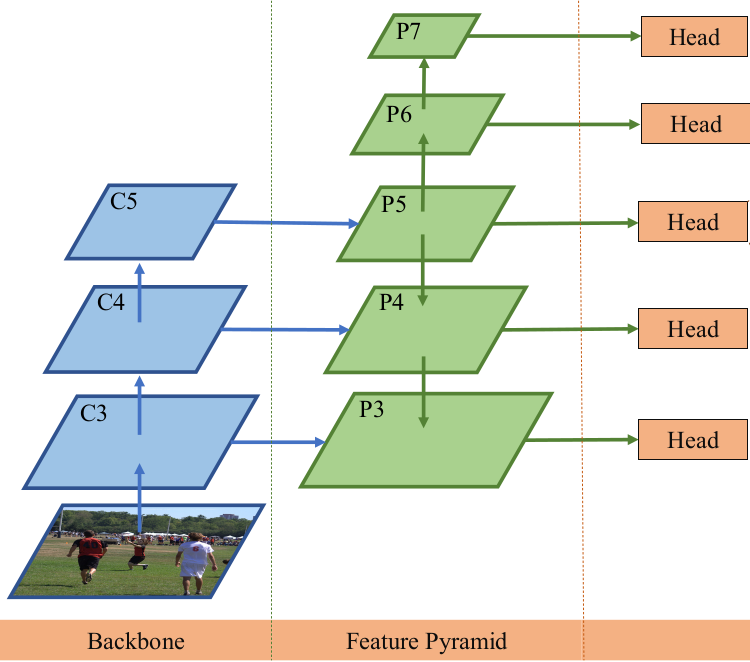
\includegraphics[width=0.6\textwidth]{chapters/internship/images/fpn.png}
	\caption[Feature pyramid network]{High-level overview of the structure of a \acrshort{fpn}. It shows a typical \acrshort{fpn} with levels P3 to P7, where P6 and P7 are built on top of P5. Arrows indicate connections, that can be of varying kind. Connections from P5 to P4 and P4 to P5 involve upsampling. This figure was taken from figure 2 in \cite{Tian:2019aaa}.}\label{fig:fpn}
\end{figure}


\section{Self-Supervised Pre-Training}\label{sec:ssl}
In this section I will introduce the concept of self-supervised learning (\acrshort{ssl}), focusing on a framework known as \emph{contrastive} learning. The goal of \acrshort{ssl} is to extract general information from raw data without labels. In the context of object detection, this data are images without any labeled objects. The hope is that the network will learn a general representation of images, which can then be fine tuned on comparatively few labeled training examples. This has the advantage of being computationally less expensive than full supervised learning, as plenty of raw data exists but labeling them is costly. Contrastive learning uses positive and negative pairs, where in the context of \acrshort{cv} positive pairs are usually different augmentations of the same image and negative pairs are augmentations of different images. The loss in this framework then encourages positive pairs to be similar and negative pairs to be dissimilar. Below I will give a brief overview of a few recent works in this field.

A framework known as SimCLR (simple framework for contrastive learnong of visual representations) was introduced in \cite{Chen:2020aab}. It consists of two networks $f$ and $g$ that operate on images $x$. The network $f$ is the core network that after fine tuning is supposed to be an image classifier, network $g$ translates the output of $f$ into a latent representation $z$. For each input two different augmentations $\tilde{x}$ and $\tilde{x}'$ are constructed and the latent representations $z$ and $z'$ are generated. For a batch of size $N$ we define $\hat{z}_{2i}=z_i$ and $\hat{z}_{2i+1}=z'$. The networks are then trained as one using the loss function
\begin{equation}
L=\frac{1}{2N}\sum_{k=1}^N\left[l\lr{2k, 2k+1} + l\lr{2k+1, 2k}\right]
\end{equation}
where,
\begin{equation}\label{eq:simclr_contrastive_loss}
l\lr{i, j}=-\log\left[ \frac{\exp\lr{s_{i,j}/\tau}}{\sum_{k=1}^{2N}\lr{1-\delta_{ki}}\exp\lr{s_{i,k}/\tau}}\right]
\end{equation}
and
\begin{equation}\label{eq:simclr_cosing_similarity}
s_{i, j} = \frac{\hat{z}_i\cdot\hat{z}_j}{\norm{z_i}\norm{z_j}}.
\end{equation}
The numerator in \eqref{eq:simclr_contrastive_loss} represents the positive pairs, whereas the denominator represents the negative pairs. The loss is minimized, when the cosine similarity \eqref{eq:simclr_cosing_similarity} for the positive pairs is minimized and for the negative pairs is maximized. The authors of \cite{Chen:2020aab} find that strong augmentations of the images improve their framework substantially and that large batch sizes ($\geq 256$) are useful. After fine tuning the network, they achieve performance almost equal to a full supervised training on ImageNet data. In a follow-up paper the authors improve on the results by utilizing very large networks~\cite{Chen:2020aac} and noticing that the larger the pre-trained model the less impactful the number of labeled images for fine tuning.

The authors of \cite{Grill:2020aaa} improve on the performance of SimCLR by introducing two branches of the same architecture. They call their approach Bootstrap Your Own Latent (BYOL) and its main advantage is that the loss does not contain any negative examples. This greatly reduces the computational cost during training, as fewer computations are required per batch sample. Instead of feeding two augmentations of the image to the same network, they introduce a second network, which is identical in architecture the first, to process the second augmentation. This setup can be understood as a teacher-student setup. Only the student is optimized directly through gradient descent, the teacher is updated by an exponential moving average of the student parameters. This procedure is also known as applying a stop-gradient to the teacher. Finally, a third network $\phi$ is introduced that is hypothesized to project the output of the student to the output of the teacher. The teacher and student produce two outputs $z$ and $z'$ for every input image and its different augmentations $x$ and $x'$, i.e. $z=g_\text{T}\lr{f_\text{T}\lr{x}}$, $z'=\phi_\text{S}\lr{g_\text{S}\lr{f_\text{S}\lr{x'}}}$, where the subscripts T and S refer to the teacher and student, respectively. The networks $f$ and $g$ serve the same roles as for SimCLR. The loss is given by a \acrshort{mse}
\begin{equation}
L=\norm{g_\text{T}\lr{f_\text{T}\lr{x}} - \phi_\text{S}\lr{g_\text{S}\lr{f_\text{S}\lr{x'}}}}^2 + \norm{g_\text{T}\lr{f_\text{T}\lr{x'}} - \phi_\text{S}\lr{g_\text{S}\lr{f_\text{S}\lr{x}}}}^2.
\end{equation}

In \cite{Chen:2020aaa} the authors present the SimSiam framework, which combines the advantages of SimCLR with those of BYOL. Their approach trains on positive pairs only and uses a stop gradient as BYOL, but does not require an exponential moving average for the teacher. They also remove the network $g$ from both approaches and are left with the network $f$ and the projector $\phi$. This greatly simplifies the overall setup for \acrshort{ssl} training and as a consequence greatly reduces the required batch sizes. While their final performance after fine tuning is weaker than that of BYOL, they manage to use less resources, which makes SimSiam viable even on modest hardware. As loss they use a negative cosine similarity.

The final \acrshort{ssl} framework I want to introduce is Selective object Contrastive learning (\acrshort{soco}) proposed in \cite{Wei:2021aaa}. Previous \acrshort{ssl} frameworks were used primarily for image classification tasks and only adapted to object detection by utilizing the pre-trained backbones. \acrshort{soco} is a \acrshort{ssl} framework specifically designed for object detection, allowing to pre-train the backbone and heads of a Mask-RCNN~\cite{He:2017aaa}. Mask-RCNN is a special Faster-RCNN that creates a pixel mask for different objects, instead of just generating bounding boxes. The proposed method is guided by the BYOL paper in the sense that it uses the three networks $f_\text{S}$, $g_\text{S}$, and $\phi_\text{S}$ for the student branch and the two networks $f_\text{T}$ and $g_\text{T}$ for the teacher, as well as using a stop gradient for the teacher and an exponential moving average to update the teacher parameters. What is called ``student'' here is named ``online network'' and what is called ``teacher'' is named ``target network'' in \cite{Wei:2021aaa}. The network $f$ is a Resnet50~\cite{He:2015aaa} with a \acrshort{fpn} attached. The \acrshort{fpn} is defined as in \cite{Lin:2017aaa} with levels P2 to P5. To adapt the BYOL framework to object detection, \acrshort{soco} produces regions of interest using the selective search algorithm~\cite{Uijlings:2013aaa}. Based on the size and location of the region proposal a corresponding area in one of the feature maps is selected and turned into a fixed size output by a layer named RoIAlign, which was introduced in \cite{He:2017aaa}. It is a special form of RoIPooling~\cite{Girshick:2015aaa} that interpolates its values to better align the input and the output. The output of the RoIAlign is then processed by the head, before being fed into the networks $g$ and $\phi$. To induce scale invariance of the object detector, the augmentation of one image is required to create a crop of the input image and resize it to the original size. Also, a third augmentation is processed, which is a downsized version of the augmented image that was cropped and resized. The loss is the sum of the cosine similarities of the output from the first augmentation with the cropped and resized augmentation and the first augmentation with the downsized version. See \autoref{fig:internship_soco} for a visualization of the framework.
\begin{figure}
	\centering
	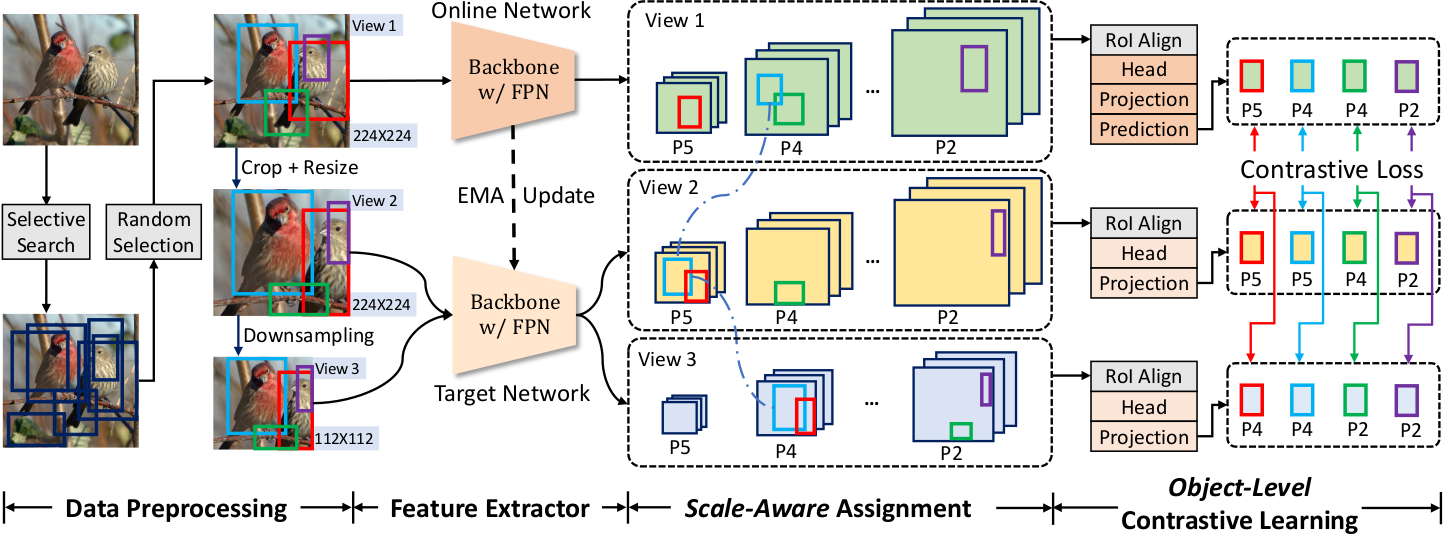
\includegraphics[width=0.98\textwidth]{chapters/internship/images/soco.png}
	\caption[Selective object Contrastive learning]{An overview of the \acrshort{soco} framework. What is called ``Online Network'' in the figure was described as student network in this chapter and what is called ``Target Network'' in the figure is the teacher network of this chapter. Different augmentations are used for view 1, 2, and 3. Different sized bounding boxes from the selective search are assigned different levels in the \acrshort{fpn}. This figure was taken from \cite{Wei:2021aaa} where it is figure 1.}\label{fig:internship_soco}
\end{figure}


\section{Research at Bosch}
At Bosch I was tasked with evaluating the usefulness of the approach called Selective object Contrastive learning (\acrshort{soco}) presented in \cite{Wei:2021aaa} to their existing object detection networks. The main challenges lay in two distinct points. First, the paper was mainly targeting two stage detectors, where the first stage samples possible regions of interest and the second stage classifies these regions. For the application that my work was targeting, anchor based single stage detectors are the prevalent approach, resulting in only portions of the architecture being able to be pre-trained using \cite{Wei:2021aaa}. Second, the code that was published~\cite{Wei:2022aaa} alongside the paper~\cite{Wei:2021aaa} needed to be validated and adapted for the networks, as well as the data used in the project.

Below I also present an adaption of the framework given in \cite{Wei:2021aaa} that I proposed to pre-train most of the single stage object detector architecture and eliminate the need to run a computationally expensive selective search \cite{Uijlings:2013aaa} before training. At the core it tries to encourage the network to create similar representations for two different augmentations of the same image. Only regions in the resulting feature maps that are present in both augmentations are compared. I evaluate the performance of a network pre-trained with this adaption, which I call \acrshort{ssdoco} (Single Shot Detector object Contrastive learning), against the same network pre-trained with the \acrshort{soco} framework.

\subsection{Introduction}
Training deep learning object detection algorithms is a difficult task. Creating classified bounding boxes as labels for the training data is far more time consuming, and therefore expensive, than creating labels that classify the entire image into a predetermined number of categories. For this reason, the interest in making un-labeled data usable for training purposes has picked up a lot of interest in the recent past~\cite{Chen:2020aab, Grill:2020aaa, Chen:2020aaa}. One of the most successful approaches so far has been a concept known as contrastive learning, which was introduced in \ref{sec:ssl}. Most of these algorithms focus on the task of image classification, where they have shown to improve performance even over full supervised training~\cite{Chen:2020aaa}. Although these algorithms are focused on image classification, they can still have a beneficial effect on object detection, as most object detection networks consist of a general backbone that aims to create a feature representation and an object detection specific part, like a feature pyramid network (\acrshort{fpn}), that tries to extract information at different scales. Afterward, classification and bounding box regression heads are attached to get the final output.

The backbone has traditionally been taken from state-of-the-art image classification algorithms~\cite{Chen:2020aab, Grill:2020aaa, Chen:2020aaa} and was always trained on image classification tasks. It is, therefore, reasonable to believe that \acrshort{ssl} pre-training algorithms devised for image classification may improve object detection algorithms, simply by improving the classification performance of the backbone.
On the other hand, object detection datasets are often different from image classification datasets. In image classification one commonly has images showing only a single object. For object detection training sets, these kinds of images are rare, and most images show multiple objects. Furthermore, additional parts of the object detection architecture, such as \acrshort{fpn}s or the detection heads, cannot be initialized from pure backbone pre-training and have to be trained from scratch on limited labeled data. To this end, it may be beneficial to develop pre-training algorithms that are tailored toward object detection, for instance by using contrastive loss functions that encourage similarity only in regions where the same objects are shown.

One of the first works presenting a \acrshort{ssl} framework that focuses on object detection is the \acrshort{soco} approach given in \cite{Wei:2021aaa}. Their goal was to pre-train the full architecture of a Mask-RCNN~\cite{He:2017aaa} that learned object level representations rather than global representations of the image. This means that rather than learning to produce similar feature maps of two different augmentations for the entire image, it focusses on producing similar representations only in regions where objects are likely to be present.

To select regions in which objects are likely to be present, \acrshort{soco} preprocesses the entire training set using a selective search \cite{Uijlings:2013aaa}, which is a generic algorithm that proposes regions of interest. This stage is computationally expensive but has to be executed only once per dataset. Whenever an image is used for training, a subset of the proposed regions is randomly selected.

In a next step, the two different augmentations of the input image are given to the two branches of their network. Both branches have the same architecture and mainly use a ResNet50 backbone~\cite{He:2015aaa} with a \acrshort{fpn}~\cite{Qiao:2021aaa}. For each selected and proposed region, the feature map that best matches the scale of the bounding box is selected and the part that corresponds to the feature map is cropped out. It is then passed to a RoIAlign layer which was introduced in\cite{He:2017aaa} to create a fixed size feature map. This can subsequently be processed by a detection head. The output of this detection head is further processed by additional layers aimed to project the output of the two branches into the same space. Finally, the output of one branch is processed by a final prediction module, that tries to translate the output of one branch to the output of the other branch. Afterward, the outputs of the two branches are compared by a cosine-similarity loss~\cite{Wei:2021aaa}.

The \acrshort{soco} framework allows to pre-train most of the Mask-RCNN architecture; backbone, \acrshort{fpn}, and classification heads. In fact, it can be easily adopted to pre-train most two stage detectors. However, adopting it to one stage detectors is not trivial. One stage detectors do a classification and bounding box regression for a fixed number of pre-determined locations in an image. Since all positions must be classified, selecting only a few of them for comparison has the potential to severely diminish the final performance.

To adapt the \acrshort{soco} framework to single stage detectors we propose \acrshort{ssdoco} (Single Shot Detector object Contrastive learning). Instead of comparing only select regions, \acrshort{ssdoco} compares compatible regions. One of the core principles of \acrshort{soco} is that one branch receives a cropped part of the original image as input to induce positional and scale invariance. \acrshort{ssdoco} uses the same concept but changes how the loss is constructed. It sums the cosine similarity loss of all compatible feature maps by cropping and interpolating the feature maps at different levels of the feature pyramid. This change allows us to effectively pre-train the entire single shot object detector, aside from the final layers.

\subsection{Methods}
We use a Retinanet~\cite{Lin:2017aaa} with a ResNet50~\cite{He:2015aaa} as backbone for our single stage object detector. The feature pyramid contains levels P3 to P7, where P6 is built from C5. For pre-training we use a single head consisting of 4 stacked convolutional layers with a kernel size of 3, 256 channels, and \acrshort{relu} activations. This architecture outputs 5 distinct feature maps of different scales. For fine-tuning both the classification head and the regression head are initialized with the weights from the single head during pre-training.

The \acrshort{ssdoco} framework follows the teacher-student model, where only the student is optimized directly using a gradient based optimizer and the teacher is updated through an exponential moving average of the student network parameters. Note that what we call the student is the ``online'' network in \cite{Wei:2021aaa} and what we call teacher is there known as the ``target'' network.

Both branches have multiple components. The student is composed of the model that should be trained, an alignment stage described below, a projector network, and a predictor network. The teacher is built the same way but does not contain a predictor network. Both the model as well as the projector of the teacher are updated by an exponential moving average of the student model and neither receive gradient updates. See \autoref{fig:internship_ssdoco} for a visualization of the framework.
\begin{figure}
	\centering
	\pgfdeclarelayer{bg}    % declare background layer
\pgfsetlayers{bg,main}  % set the order of the layers (main is the standard layer)
\begin{tikzpicture}[square/.style={regular polygon,regular polygon sides=4, draw, minimum width=2.4cm, fill=white}]
    \pgfmathsetmacro{\vsepa}{0.35}
    \node (img1) {Img 1};
    \node[below=2.4cm of img1] (img2) {Img 2};

    \node[square, right=.8cm of img1] (bbs) {BB};
    \node[square, right=.8cm of img2] (bbt) {BB};

    \node[square, right=\vsepa cm of bbs] (fpns) {\acrshort{fpn}};
    \node[square, right=\vsepa cm of bbt] (fpnt) {\acrshort{fpn}};

    \node[square, right=\vsepa cm of fpns] (as) {Align};

    \node[square, right=\vsepa cm of as] (projs) {Proj.};
    \draw (fpnt -| projs) node[square] (projt) {Proj.};

    \node[square, right=\vsepa cm of projs] (pred) {Pred.};

    \coordinate (h1) at ($(projs)!0.5!(projt)$);
    \node (contrast) at ($(h1 -| pred.east)+(.4, 0)$) {Contrast};

    \draw[->] (img1.south) -- (img2.north);
    \node[text width=2cm] at ($(img1.south)!0.5!(img2.north)+(1.2, 0)$) {Crop +\newline Resize};

    \draw[->] (bbs.south) -- (bbt.north);
    \node at ($(bbs.south)!0.5!(bbt.north)+(0.6, 0)$) {EMA};

    \draw[->] (fpns.south) -- (fpnt.north);
    \node at ($(fpns.south)!0.5!(fpnt.north)+(0.6, 0)$) {EMA};

    \draw[->] (projs.south) -- (projt.north);
    \node at ($(projs.south)!0.5!(projt.north)+(0.6, 0)$) {EMA};

    \draw[->] (img1.east) -- (bbs.west);
    \draw[->] (bbs.east) -- (fpns.west);
    \draw[->] (fpns.east) -- (as.west);
    \draw[->] (as.east) -- (projs.west);
    \draw[->] (projs.east) -- (pred.west);
    \draw[->] (pred.east) -| (contrast.north);

    \draw[->] (img2.east) -- (bbt.west);
    \draw[->] (bbt.east) -- (fpnt.west);
    \draw[->] (fpnt.east) -- (projt.west);
    \draw[->] (projt.east) -| (contrast.south);

    \node (augs) at ($(img1.east)!0.5!(bbs.west)+(-0.1, 0.3)$) {Aug};
    \node (augt) at ($(img2.east)!0.5!(bbt.west)+(-0.1, 0.3)$) {Aug};

    \draw[->] (augs.north) -- ++(0, 1) -| (as.north);

    \begin{pgfonlayer}{bg}    % select the background layer
        \draw[rounded corners, dashed, red, fill=red, fill opacity=.2] ($(bbs.north west)+(-.1, .1)$) rectangle ($(pred.south east)+(.1, -.1)$);

        \draw[rounded corners, dashed, blue, fill=blue, fill opacity=.2] ($(bbt.north west)+(-.1, .1)$) rectangle ($(projt.south east)+(.1, -.1)$);
    \end{pgfonlayer}

    \node[red] at ($(projs.north)+(.5, .5)$) {\textbf{Student}};
    \node[blue] at ($(projt.south)+(-1.9, .3)$) {\textbf{Teacher}};

    \node[minimum width=2.cm, right=\vsepa cm of projt] (sg) {
        \begin{tikzpicture}[anchor=0]
            \draw (-0.42, -.5) -- (.18, .5);
            \draw (-.18, -.5) -- (.42, .5);
        \end{tikzpicture}
    };
    \node at ($(sg.south)+(-.1, -.1)$) {stop-grad};
\end{tikzpicture}
	\caption[SSDoCo framework]{An overview of the \acrshort{ssdoco} framework. ``Img 1'' is an input image and ``Img 2'' is constructed from it by cropping and resizing to the original resolution. Each image subsequently gets its own augmentation ``Aug'', before being passed through the backbone ``BB'' and the \acrshort{fpn}. The ``Align'' step selects and interpolates the parts of the feature maps that are visible in ``Img 2''. The networks ``Proj.'' and ``Pred.'' are the projection and prediction networks. Finally, the contrastive loss is computed for both branches and the gradient is propagated back through the student. The parameters of the teacher are updated as an exponential moving average ``EMA'' of the student parameters.}\label{fig:internship_ssdoco}
\end{figure}

The two branches receive different augmentations of the same image. We follow \cite{Wei:2021aaa} for the choice of augmentations, but do not construct a “View 3”. The exact transformations are listed in \autoref{tab:transformations_ssdoco}. The teacher receives a random sub-view of the input to the student, the area of which is randomly selected between $50\%$ and $100\%$. The sub-view is subsequently resized to the original image size using bilinear interpolation. To enforce symmetry, we swap the inputs of the student and teacher after the forward pass and compute the loss as a sum of both results.
\begin{table}
\begin{tabularx}{\textwidth}{|p{0.02\textwidth}|X|p{0.276\textwidth}|X|p{0.06\textwidth}|X|p{0.06\textwidth}|}
\hline
\# & Name & Description & \multicolumn{2}{c|}{Student} & \multicolumn{2}{c|}{Teacher}\\
\cline{4-7}
& & & Params & Prob & Params & Prob \\
\hline
1 & Resize & Resize smaller side to 224 pixels & $-$ & $1$ & $-$ & $1$ \\
\hline
2 & Crop & Random crop to 224x224 pixels & $-$ & $1$ & $-$ & $1$ \\
\hline
3 & Random Crop + Resize & Random square crop and resize to 224x224 pixels & $-$ & $0$ & scale from $0.5$ to $1$ & $1$ \\
\hline
4 & Horizonal Flip & Flip image horizontally & $-$ & $0.5$ & $-$ & $0.5$ \\
\hline
5 & Color Jitter & Apply various color transformations & brightness $0.4$\newline contrast $0.4$\newline saturation $0.2$\newline hue $0.1$ & $0.8$ & brightness $0.4$\newline contrast $0.4$\newline saturation $0.2$\newline hue $0.1$ & $0.8$ \\
\hline
6 & Grayscale & Convert image to Grayscale & $-$ & $0.2$ & $-$ & $0.2$ \\
\hline
7 & Gaussian Blur & Blur the image & sigma from $0.1$ to $2$ kernel size $15\times 15$ & $1$ & sigma from $0.1$ to $2$ kernel size $15\times 15$ & $0.2$ \\
\hline
8 & Solarize & Solarize image & Threshold $128/255$ & $0.2$ & $-$ & $0$ \\
\hline
9 & Norm & Normalize the input data & Mean: $0.5$\newline Std: $0.225$ & $1$ & Mean: $0.5$\newline Std: $0.225$ & $1$ \\
\hline
\end{tabularx}
\caption[Transformations]{The image augmentations used for the \acrshort{ssdoco} training. The ``Prob'' columns give the probability of applying the given transformation.}\label{tab:transformations_ssdoco}
\end{table}

For the loss we use a variant of cosine similarity, which we shift and scale to return values between 0 and 2. The loss is given by
\begin{equation}
L\lr{y_1, y_2} = 2 + \frac{1}{n}\sum_{i=1}^n\text{L2}\lr{y_1^i, y_2^i},
\end{equation}
where $y_x$ is the output of model $x$, and $y_x^i$ is output $i$ of model $x$. The function L2 is given by
\begin{equation}
\text{L2}\lr{y_1, y_2} = -2\frac{y_1\cdot y_2}{\norm{y_1}\cdot\norm{y_2}}.
\end{equation}
However, naively comparing the five different feature maps would yield inconsistent results, as the input images are at different scales and show different regions of the same image. For this reason, we compare only those feature maps that are on similar scale and project the feature maps that were derived on the full image onto the sub-region given to the other branch of the Siamese network.

The feature pyramid in the network is built such that the scale of the features double at each level. We, therefore, enumerate the five output feature maps from smallest scale (i.e. largest feature map) to largest scale (i.e. smallest feature map). We then compare feature map $j+i$ of the unscaled image with feature map $j$ of the scaled image, where $i$ is given by
\begin{equation}
i=\lfloor\log_2\lr{s}\rfloor,
\end{equation}
with $1/s$ being the scale chosen in the Random Crop + Resize transformation. The index $j$ ranges from $0$ to $n-i$, where $n$ is the number of feature maps, i.e. 5. Our settings are chosen such that $1<s<2$ and, therefore, $i=0$. Consequently, we always compare the same levels of feature maps and only have to take care of the projection.

For the projection we interpret each pixel of the feature map as if it is associated to an anchor box in the input image. We then transform the anchor box-coordinates in the scaled branch to their (sub-pixel) position in the un-scaled image. This process takes re-scaling, cropping boundaries, and horizontal flips into account. We then interpolate the feature map of the un-scaled branch at those transformed coordinates, to obtain a comparable grid. We use bilinear interpolation. Afterward the feature maps are flattened, and the cosine similarity loss described above is applied.

\subsection{Experiments}
All pre-training uses a set of $1.6$ million diverse unlabeled images taken from Flickr~\cite{Flickr:2022aaa}. The data set was created internally to test the influence of large data sets which show widely differing scenes that are not specific to the final domain the network should operate on.

Once the pre-training is finished, all networks are fine tuned on the same set of labeled data. This set is also sampled from Flickr and contains $5\,500$ images. For each epoch, $5\,000$ batches are randomly sampled from the set and the network is trained for $40$ epochs with a batch size of $8$ or $80$ epochs with a batch size of $4$, depending on memory limitations of the hardware.

To compare the performance, we report the log average miss rate (\acrshort{lamr}) averaged over all six classes. We use the Caltech protocol given in \cite{Dollar:2012aaa} to determine true and false positives. The miss rate is averaged over five different false positive rates, where the false positive rate is given in terms of false positives per image. The miss rate is the number of false negatives divided by the number of ground truth boxes. Averaging over multiple false positive rates gives a more stable estimate of the detector performance. Lower values of the log average miss rate indicate better performance.

As baseline we fine tuned the network from random initialization. We found that the minimum \acrshort{lamr} after 40 epochs was $\approx 53\%$. To find any improvement, this baseline has to be beaten. Furthermore, we used ImageNet pre-trained weights as initialization for the backbone only. The \acrshort{fpn} and heads were initialized randomly. In this setup we found a minimal \acrshort{lamr} of $\approx 33\%$.

\subsubsection{SoCo}
We adjusted the code published alongside the \acrshort{soco} paper~\cite{Wei:2022aaa} to use the Retinanet discussed above. However, we removed the heads from the Retinanet and only replaced the backbone and \acrshort{fpn}, as both components differ to the original implementation only in minor details. The greatest difference is the inclusion of the levels P6 and P7, which were dropped from the original work due to the size of the resulting feature maps. Our network uses the outputs $\left\{\text{P3}, \text{P4}, \text{P5}, \text{P6}, \text{P7}\right\}$. Consequently, we also had to adjust the awareness scales. We define object proposals of area within the range of $\left\{0-48^2,49^2-96^2,97^2-192^2,193^2-208^2,209^2-224^2\right\}$ pixels to $\left\{\text{P3}, \text{P4}, \text{P5}, \text{P6}, \text{P7}\right\}$, respectively. Due to hardware limitations we also had to lower the batch size to $64$ samples.

Before training, we applied the selective search to the entire training set. To reduce runtime, we resized all images such that the smaller side has a size of $224$ pixels, before applying selective search. Afterward, the boxes were scaled to match the original image size.

We pre-trained the architecture for $10$ epochs with a warmup of $1$ epoch using the same LARS optimizer~\cite{You:2017aaa} and settings as given in the \acrshort{soco} repository~\cite{Wei:2022aaa}. We found that the outputs of the network grow during pre-training. This forced us to not use mixed precision training during fine tuning and, therefore, reduce the batch size to $4$. This fine tuning seemed to be unstable and only converging occasionally. When the fine tuning converged, performance was on the order of a randomly initialized network.

To make sure that the architecture was not a problem, we changed the backbone and \acrshort{fpn} to match those cited in the paper~\cite{Wei:2021aaa}. We also changed the association of the area of proposals with \acrshort{fpn} levels back to the original implementation. However, pre-training and fine tuning showed the same problem as before, with the network converging only sometimes. Converged networks could not beat a random initialization during fine tuning.

When we fine tune the network, we only initialize those parts of the network that have had pre-training. The remaining weights and biases are initialized randomly. This means that the P6 and P7 levels are initialized randomly in our second experiment during fine tuning. In both cases, we tested initializing both the backbone and the \acrshort{fpn} as well as only the backbone. Neither option yielded any improvements over the other.

\subsubsection{SSDoCo}
To evaluate the SSDoCo approach, we tested multiple different ideas aimed at improving performance. All tests use the same backbone and \acrshort{fpn} of the Retinanet, but the projector and predictor were varied. We also experimented with different optimizers and regularization techniques.

Initially, following the architecture of SimSiam~\cite{Chen:2020aaa}, the projectors were removed and the predictors for the different feature maps were $1\times 1$ convolutions that only altered the channel dimension. We trained the network with the Adam~\cite{Kingma:2014aaa} optimizer. The transformation aligning the outputs was placed after the output of the predictor. These experiments showed that the output was continually growing, the longer we trained. This caused fine tuning to be unstable and diverge. Consequently, we introduced L2 regularization~\cite{Ng:2004aaa}, to reduce the numerical values of the weights and, thereby, the output. We also switched to the LARS~\cite{You:2017aaa} optimizer, following the recommendations of the \acrshort{soco} paper.

After these alterations, the network output stayed on average below 1. However, the loss quickly fell during the first few batches and continued to grow afterward. This problem was rectified by lowering the initial learning rate by an order of magnitude. The resulting algorithm trained smoothly but checking the outputs for different inputs revealed that the output was constant for different inputs.

We initially tried to force the network to avoid collapsing to constant outputs by introducing a new regularization term to the loss. This term penalizes low weight variance and is given by
\begin{equation}
L\lr{\theta}=\frac{1}{N}\sum_{i=1}^N\lr{s\text{Var}\left[\theta_i\right]+\epsilon}^{-1},
\end{equation}
where $s$ is a scale factor, $\epsilon$ is a small constant, and $\theta_i$ are the parameters of layer $i$. The function Var calculates the variance of the parameters. After some experiments we found that this regularization seems to solve the problem. However, fine tuning resulted in a network that is on par with a randomly initialized network.

To align the \acrshort{ssdoco} training more strongly with both the \acrshort{soco} training and previous \acrshort{ssl} pre-training experience, we introduced a projector using global average pooling, followed by two dense layers. The predictor was altered to consist of two dense layers, where the first is a bottleneck, i.e. having fewer neurons than its input and the subsequent output. We also moved the transformation aligning the outputs of the teacher and the student to take place between the Retinanet and the projector. So, the student is composed of a Retinanet, followed by the output alignment, the projector, and finally the predictor. The teacher network has the same structure but drops the predictor. Both the Retinanet and the projector of the teacher are updated through an exponential moving average of the student.

Aligning the setup with previous experience, the output dropped to expected small scales. However, fine tuning still did not produce a network that could beat a random initialization.

We also tried fine tuning all architectures by initializing only the backbone and \acrshort{fpn} of the network with the pre-trained weights. This had proven helpful in other scenarios. However, this could not improve fine tuning results either.

We had planned to test the influence of the batch size, the size of the bottleneck layer, and the influence of different data set sizes on the final performance of the algorithm. Due to a missing baseline, we could not perform these experiments.

Pre-training was carried out on four NVIDIA A6000 GPUs for a total batch size of $128$. Training for $10$ epochs on $1.6$ million images required about 4 days. We used a learning rate of $0.1$ and a momentum of $0.9$ in the LARS optimizer. We used the same weight decay implementation and settings as given in \cite{Wei:2022aaa}.

\subsection{Conclusions}
We have tested the \acrshort{soco} framework presented in \cite{Wei:2021aaa} and a custom extension of it – named \acrshort{ssdoco} – on a diverse dataset. Our goal was to pre-train a Retinanet for complex object detection tasks on a large unlabeled dataset and fine tune it on application specific data. The frameworks allowed to pre-train both the backbone as well as the \acrshort{fpn}, while the \acrshort{ssdoco} approach was envisioned to also allow pre-training of the detection- and classification-heads.

We found that neither of the two contrastive pre-training methods managed to produce network parameters that could beat a random initialization during a fixed fine tuning. Especially, the findings of \acrshort{soco} could not be reproduced on our data. We hypothesize that this could be due to two reasons. First, our datasets contain many objects, compared to MS Coco~\cite{Lin:2014aaa}, which was used in \acrshort{soco}. This could be challenging for a framework that tries to align object views. Second, limited hardware resources restricted the batch size we could use during pre-training to $64$ samples. The lowest batch size results are reported on in \cite{Wei:2021aaa} is $512$; a $8$ times increase over our setup.

The \acrshort{ssdoco} setup allowed us to train with a batch size of $128$. The training produced much more stable results, that managed to converge every time during fine tuning. However, the performance after fine tuning could not outperform random initialization. Given that the \acrshort{soco} framework, which the \acrshort{ssdoco} approach is loosely based on, did not produce positive results on our datasets, we believe it to be unlikely that \acrshort{ssdoco} will yield tangible performance benefits. However, other \acrshort{ssl} methods have already proven to be successful, which justifies further research in this area.


\chapter{Conclusions and Outlook}\label{ch:conclusions}
This thesis has analyzed the applicability of \acrshort{ml} methods to the problem of detecting \acrshort{gw} signals from \acrshort{cbc} sources in comparatively strong noise. It studied both \acrshort{bns} and \acrshort{bbh} signals and introduced novel methods to expand the capabilities of existing \acrshort{ml} algorithms. A core contribution of this thesis is an objective comparison of sensitivities between \acrshort{ml} methods and existing search pipelines. Several studies highlighted the importance of calculating sensitivities normalized by the population of \acrshort{gw} sources derived from long-duration continuous data to make representative claims about \acrshort{gw} detection capability.

Each chapter of this thesis has solved select problems of \acrshort{ml} based searches for \acrshort{cbc} signals to advance the field from a proof of principle level to actual applications. Chapter \ref{ch:bns} introduced a novel deep learning based search for \acrshort{bns} signals that outperforms previous \acrshort{ml} methods at low \acrshort{far}s. While it is not yet competitive with matched filter searches, it provides a method to reduce the number of data samples that need to be processed. This reduction in data size for \acrshort{bns} signals is crucial for \acrshort{nn}s, as they struggle with large inputs. Chapter \ref{ch:training_strats} introduced a simple modification to the \acrshort{nn}s used in early deep learning \acrshort{bbh} search algorithms. This extension enabled the algorithm to operate at \acrshort{far}s $\mathcal{O}(1)$ per month and be competitive to a matched filter baseline. Chapter \ref{ch:cnn_coinc} applied a coincidence strategy to deep learning searches optimized on a single detector and showed that the background can be trivially extended to test the algorithm down to \acrshort{far}s $\mathcal{O}(10^{-2})$ per year. Chapter \ref{ch:mlgwsc1} presents the results of a global mock data challenge organized by the author of this thesis. The mock data challenge makes the tools and experiences gained from chapters \ref{ch:bns} to \ref{ch:cnn_coinc} publicly available by publishing open source software and reference data sets that can be used to evaluate any search on the provided parameter space. The evaluation results can be compared to existing literature, as the study includes reference sensitivities from current production search pipelines.

The summarized takeaways from the various analyses presented in this thesis are as follows. \acrshort{nn}s are already competitive in sensitivity to matched filtering when \acrshort{bbh} signals are considered. This is highlighted by the results found in chapter \ref{ch:mlgwsc1}. There, the best \acrshort{ml} search retains $\geq 70\%$ of the sensitivity achieved by the state-of-the-art matched filter based PyCBC search pipeline and becomes comparable at \acrshort{far}s $> 100$ per month, even in real noise. However, while the most sensitive algorithm requires less time to process the data than PyCBC, the probed parameter region is still efficiently searched by existing methods. In regions of parameter space, where matched filtering becomes computationally more expensive, deep learning is also limited in its capability. Especially long duration \acrshort{bns} and \acrshort{nsbh} signals are still challenging to \acrshort{nn} searches. This is in line with chapter \ref{ch:bns} where we observed that, while we improve the state-of-the-art for deep learning \acrshort{bns} searches, our algorithm is handily outperformed by matched filtering. We also found evidence of the same problem in chapter \ref{ch:mlgwsc1}, where even high \acrshort{snr} long duration signals were missed by all deep learning searches. Furthermore, the results presented in chapter \ref{ch:cnn_coinc} suggest that a major problem for \acrshort{ml} algorithms in the future may be the unavailability of signal consistency tests to reject many noise artifacts. Typically deep learning searches are used as binary classifiers that decide only between the presence and absence of a signal in the parameter region they were trained on. The lack of crude source parameter estimates in this setting complicates a coincidence analysis, which greatly decreases the \acrshort{far}s that can be trivially tested.

Challenges for \acrshort{ml} based \acrshort{gw} search algorithms are plentiful, but should not be discouraging. Great progress has been made in the last few years in terms of capability and clarity of results. Their enormous potential, the rapid development of deep learning methods that can be imported from other research areas, and the easy utilization of graphics cards are all good reasons to continue trying to overcome existing problems. Furthermore, some \acrshort{ml} algorithms are already invaluable tools in some areas of \acrshort{gw} astronomy. These include glitch classification~\cite{Zevin:2016qwy} and improvements to ranking statistics to reject non-Gaussian noise artifacts~\cite{Mishra:2021tmu}.

The identified weaknesses of current approaches also provide a clear path for future research. It is necessary to develop \acrshort{ml} algorithms capable of reliably and rapidly detecting weak, long duration \acrshort{gw}s from sources such as \acrshort{bns} or \acrshort{nsbh} mergers. These sources are of special interest as they potentially emit an \acrshort{em} counterpart, which can be used to extract further information from the system and constrain stellar models. Their rapid detection can increase the \acrshort{em} observation time, hopefully to a point where the prompt emission can be observed. It is also desirable to develop \acrshort{ml} \acrshort{gw} searches that operate at low \acrshort{far}s on the order of one per year. A promising route studied in this thesis is the adoption of a coincidence analysis scheme as it is used by state-of-the-art production searches. To achieve this goal and reliably reject non-Gaussian noise artifacts, developing signal consistency checks for deep learning based algorithms is important. Organizing future mock data challenges would be beneficial to benchmark the progress of the field accurately. The mock data challenge discussed in chapter \ref{ch:mlgwsc1} has provided a baseline that can be easily extended to more difficult regions of parameter space.

Beyond the clear path painted by the challenges of existing methods identified in this thesis, there are further interesting avenues to apply \acrshort{ml} in \acrshort{gw} astronomy. One approach to utilize \acrshort{ml} in \acrshort{gw} detection that has often been proposed but never actually been explored beyond an initial study~\cite{Verma:2021epx} is to do a hierarchical search. Fast \acrshort{ml} algorithms can be used to flag candidate detections at high \acrshort{far}s, thereby rejecting most of the noise. The candidate detections can then be checked using matched filtering to reduce computational costs while preserving the sensitivity of state-of-the-art analyses. The work in this thesis has already proven that deep learning searches can be more sensitive than matched filtering at very high \acrshort{far}s and may, therefore, be great first-stage filters. Another application not explored in this thesis that has gathered much interest in the recent past is the rapid production of posteriors to determine the parameters of \acrshort{gw} sources~\cite{Gabbard:2019rde, Dax:2021tsq}. Such development could reduce the computational costs by orders of magnitude due to the long runtimes of existing parameter estimation codes and the trivial evaluation of their deep learning counterparts.

Future \acrshort{gw} observation runs and detectors are expected to provide an increased rate of detections. The increased number of observations will allow us to make more reliable statements about the population of astrophysical objects and hopefully lead to new and exciting insights into the Universe. At the same time, the large number of expected detections provides a challenge for data analysts that need to process them in a timely manner. This is where \acrshort{ml} algorithms may be able to provide solutions previous algorithms cannot. How effective \acrshort{ml} algorithms will be applied in broad \acrshort{gw} astronomy tasks and how strongly they will be utilized remains to be seen. However, this thesis shows that \acrshort{ml} has already passed many of the hurdles needed for an application as a \acrshort{gw} search pipeline.


\printbibliography[heading=bibintoc]

\appendix

\chapter{Acknowledgments}
Throughout the three years that I have spent working on this thesis I had support from many people, who I would like to thank here.

First of, I would like to thank the entire Albert-Einstein-Institute for their support, the opportunities they have provided me with, and the friendly working environment. The discussions I could partake in were always very fruitful. I specifically want to thank Bruce Allen, Alexander Harvey Nitz, and Badri Krishnan for allowing me to join the institute and the compact binary merger group. I also want to thank the Atlas computing team at the Albert-Einstein-Institute for their support, without whom most of the work presented in this thesis would not have been possible.

I am especially grateful for the guidance I have received by Alexander Harvey Nitz, who in most aspects has been my mentor. He suggested many of the research topics covered in this thesis but was also always open to new ideas and allowed me to experiment. His insights and tips have been invaluable to the completion of this thesis.

Another person who has greatly influenced my scientific evolution is Frank Ohme. He was my first point of contact with the Albert-Einstein-Institute and has always tried to enable my development wherever possible. His scientific input has greatly improved the quality of the works presented in this thesis.

I would also like to thank all co-authors of the various publications that have culminated in this thesis. These people are Bernd Br{\"u}gmann, Miriam Cabero, Zhoujian Cao, Collin D. Capano, Elena Cuoco, Tito Dal Canton, Rahul Dhurkunde, Zong-Kuan Guo, Eliu A. Huerta, Panagiotis Iosif, Shilpa Kastha, Sergey Klimenko, Alexandra E. Koloniari, Sumit Kumar, Chris Messenger, Tanmaya Mishra, Alexander H. Nitz, Paraskevi Nousi, Frank Ohme, Nikolaos Passalis, Zhixiang Ren, Francesco Salemi, Nikolaos Stergioulas, Anastasios Tefas, Gabriele Vedovato, He Wang, Yi-Fan Wang, Shichao Wu, and Ond{\v{r}}ej Zelenka.

A major contribution to the completion of this thesis have been my family and my close friends. Their moral and emotional support has been essential for my well being during this time. Most importantly I want to express my gratitude towards my mother Marie Therese Schäfer and my partner Nadine Speer, who were a pillar especially during difficult times. I also want to thank my father Thomas Eberhard Kurt Schäfer as well as Doris Maria Schulz, Helmger Hans Roderich Schotola, Felizitas Kaya, Horst Paul Hermann Schrödter, and Brigitta Beatrice Kuhr for support during all stages of my life.

I would further like to thank Bosch Hildesheim for allowing me to have a look into the non-academic work life and for interesting insights into computer vision applications of deep learning. I would like to especially thank Niklas Beuter, Hendrik Klose, and Christoph Dreißigacker, who made the internship possible. Furthermore, I would like to thank Lukas Enderich, who I closely worked with, as well as the entire closed loop learning project for the warm welcome and the open discussions.

Finally, I would like to thank the people who proofread the majority of this thesis. They significantly improved clarity, grammar, and spelling. Thank you Tobias Blenke, Christoph Dreißigacker, Lukas Enderich, Tom Junker, Alexander H. Nitz, Frank Ohme, Lina Schmitz, Nadine Speer, and Ond\v{r}ej Zelenka.


\chapter{List of Publications}\label{app:publications}
The research for this thesis has resulted in the following publications:
\begin{itemize}
	\item[\cite{Schafer:2020kor}] Marlin B. Schäfer, Frank Ohme, and Alexander H. Nitz, \href{https://doi.org/10.1103/PhysRevD.102.063015}{Detection of gravitational-wave signals from binary neutron star mergers using machine learning.} Phys. Rev. D 102.6 (2020)
	\item[\cite{Nitz:2020vym}] Alexander H. Nitz, Marlin B. Schäfer, and Tito Dal Canton, Forecasting \href{https://doi.org/10.3847/2041-8213/abbc10}{Gravitational-wave Merger Forecasting: Scenarios for the Early Detection and Localization of Compact-binary Mergers with Ground-based Observatories.} Astrophys. J. Lett. 902 (2020)
	\item[\cite{Nitz:2021uxj}] Alexander H. Nitz, Collin D. Capano, Sumit Kumar, Yi-Fan Wang, Shilpa Kastha, Marlin B. Schäfer, Rahul Dhurkunde and Miriam Cabero, \href{https://doi.org/10.3847/1538-4357/ac1c03}{3-OGC: Catalog of Gravitational Waves from Compact-binary Mergers.} Astrophys. J. 922.1 (2021)
	\item[\cite{Schafer:2021fea}] Marlin B. Schäfer and Ond\v{r}ej Zelenka, Alexander H. Nitz, Frank Ohme and Bernd Brügmann, \href{https://doi.org/10.1103/PhysRevD.105.043002}{Training strategies for deep learning gravitational-wave searches.} Phys. Rev. D 105.4 (2022)
	\item[\cite{Schafer:2021cml}] Marlin B. Schäfer and Alexander H. Nitz, \href{https://doi.org/10.1103/PhysRevD.105.043003}{From one to many: A deep learning coincident gravitational-wave search.} Phys. Rev. D 105.4 (2022)
	\item[\cite{Nitz:2021zwj}] Alexander H. Nitz, Sumit Kumar, Yi-Fan Wang, Shilpa Kastha, Shichao Wu, Marlin B. Schäfer, Rahul Dhurkunde and Collin D. Capano, \href{http://arxiv.org/abs/2112.06878}{4-OGC: Catalog of gravitational waves from compact-binary mergers.} pre-print arXiv: 2112.06878 (2021)
	\item[\cite{Schafer:2022dxv}] Marlin B. Schäfer, Ond\v{r}ej Zelenka, Alexander H. Nitz, He Wang, Shichao Wu, Zong-Kuan Guo, Zhoujian Cao, Zhixiang Ren, Paraskevi Nousi, Nikolaos Stergioulas, Panagiotis Iosif, Alexandra E. Koloniari, Anastasios Tefas, Nikolaos Passalis, Francesco Salemi, Gabriele Vedovato, Sergey Klimenko, Tanmaya Mishra, Bernd Brügmann, Elena Cuoco, E.A. Huerta, Chris Messenger and Frank Ohme, \href{http://arxiv.org/abs/2209.11146}{MLGWSC-1: The first Machine Learning Gravitational-Wave Search Mock Data Challenge.} pre-print arXiv: 2209.11146 (2022)
\end{itemize}

{
\titleformat{\chapter}{\Huge\bfseries}{}{0pt}{}
\titlespacing{\chapter}{0pt}{-20pt}{0pt}

\chapter{Curriculum Vitae}
{\noindent\Large Marlin Benedikt Schäfer}
\vspace*{1cm}

\vspace*{-0.5cm}
\noindent
\begin{tabular}{ll}
\textbf{Date of birth} & 28th December 1995 \\
\textbf{Place of birth} & Hannover, Germany \\
\textbf{Email} & marlin.schaefer@aei.mpg.de
\end{tabular}

\vspace*{-0.5cm}
\section*{Education}
\vspace*{-0.5cm}
{\renewcommand{\arraystretch}{1.25}
\begin{tabularx}{\textwidth}{lX}
\textbf{2017 -- 2019} & MSc Physik -- Leibniz Universität Hannover\\
 & Master thesis\\
 &
 	{
 	\begin{tabularx}{\linewidth}{X}
 		Analysis of Gravitational-Wave Signals from Binary Neutron Star Mergers Using Machine Learning\\
 		Supervisor: Dr. Frank Ohme
 	\end{tabularx}
 	}\\
\textbf{2014 -- 2018} & BSc Physik -- Leibniz Universität Hannover\\
 & Bachelor thesis\\
 &
 	{\begin{tabularx}{\linewidth}{X}
 		 Massenbestimmung kompakter Binärsysteme durch Analyse von Gravitationswellen\\
 		 Determination of Component Masses from Compact Binary System by Analyzing Gravitational Waves \\
 		 Supervisor: Prof. Domenico Giulini
	\end{tabularx}}\\
\textbf{2006 -- 2014} & Abitur -- Kaiser-Wilhelm- und Ratsgymnasium Hannover
\end{tabularx}
}

\vspace*{-0.5cm}
\section*{Experience}
\vspace*{-0.5cm}
\begin{tabularx}{\textwidth}{lX}
\textbf{Nov. 2019 -- Dec. 2022} & Doctoral researcher -- Albert-Einstein-Institute Hannover\\
\textbf{Jun. 2022 -- Sep. 2022} & Research intern -- Robert Bosch GmbH Hildesheim\\
\textbf{Apr. 2019 -- Sep. 2019} & Assistant researcher -- Albert-Einstein-Institute Hannover\\
\textbf{Oct. 2016 -- Mar. 2019} & Tutor for theoretical physics -- Leibniz Universität Hannover\\
\textbf{Aug. \& Sep. 2016 -- 2018} & Tutor for mathematics -- Leibniz Universität Hannover
\end{tabularx}
}

\end{document}